\documentclass{article}
\pdfoutput=1

%%% Packages %%%

\usepackage[moderate,margins=normal,leading=normal]{savetrees}

% Graphics
\usepackage{graphicx}
\usepackage[caption=false,font=footnotesize]{subfig}

% Formatting
\usepackage{color}
\usepackage{amsmath}
\usepackage{amsfonts}
\usepackage{bbm}
\usepackage[nodisplayskipstretch]{setspace}

\usepackage[scaled]{helvet}
\renewcommand*\familydefault{\sfdefault} %% Only if the base font of the document is to be sans serif
\usepackage[T1]{fontenc}

% Environments
\usepackage{IEEEtrantools}
\usepackage{algorithm}
\usepackage{algorithmic}

% Logic
\usepackage{ifthen}
\usepackage{etoolbox}

% References
\usepackage{natbib}

% Drawing
\usepackage{tikz}
\usepackage{pgfplots}
 \usetikzlibrary{plotmarks}
 \pgfplotsset{compat=newest}
 \pgfplotsset{plot coordinates/math parser=false}
 \usepgfplotslibrary{external}
 \tikzexternalize[prefix=tikz/]

\graphicspath{{figures/}}

%%% Macros %%%
%%% Theorem environments %%%
\newtheorem{theorem}{Theorem}[section]
\newtheorem{lemma}[theorem]{Lemma}
\newtheorem{proposition}[theorem]{Proposition}
\newtheorem{corollary}[theorem]{Corollary}
\newtheorem{model}[theorem]{Model}

\newenvironment{proof}[1][Proof]{\begin{trivlist}
\item[\hskip \labelsep {\bfseries #1}]}{\end{trivlist}}
\newenvironment{definition}[1][Definition]{\begin{trivlist}
\item[\hskip \labelsep {\bfseries #1}]}{\end{trivlist}}
\newenvironment{example}[1][Example]{\begin{trivlist}
\item[\hskip \labelsep {\bfseries #1}]}{\end{trivlist}}
\newenvironment{remark}[1][Remark]{\begin{trivlist}
\item[\hskip \labelsep {\bfseries #1}]}{\end{trivlist}}

\newcommand{\qed}{\nobreak \ifvmode \relax \else
      \ifdim\lastskip<1.5em \hskip-\lastskip
      \hskip1.5em plus0em minus0.5em \fi \nobreak
      \vrule height0.75em width0.5em depth0.25em\fi}
%%%%%%%%%%%%%%%%%%%%%%%%%%%%%%


\newcommand{\real}{\mathbb{R}}

\newcommand{\lhood}{l}
\newcommand{\nconst}[1]{K_{#1}}

\newcommand{\lsspace}{\mathcal{X}}
\newcommand{\lsdim}{{d_{\ls{}}}}
\newcommand{\priorden}{p}
\newcommand{\postden}{\pi}
\newcommand{\seqden}[1]{\pi_{#1}}
\newcommand{\seqdenapprox}[1]{\hat{\pi}_{#1}}
\newcommand{\impden}{q}
\newcommand{\incimpden}[1]{q_{#1}}

\newcommand{\logprior}{M}
\newcommand{\loglhood}{L}
\newcommand{\logseqden}[1]{\Xi_{#1}}
\newcommand{\logseqdenapprox}[1]{\hat{\Xi}_{#1}}

\newcommand{\sn}[1]{z_{#1}}
\newcommand{\snchange}[1]{\xi_{#1}}

\newcommand{\lsmnapprox}[1]{\hat{m}_{#1}}
\newcommand{\lsvrapprox}[1]{\hat{P}_{#1}}


% Particle flow
\newcommand{\flowbm}[1]{\epsilon_{#1}}          % Particle flow Brownian motion
\newcommand{\flowdrift}[1]{\zeta_{#1}}          % Particle flow drift
\newcommand{\flowdiffuse}[1]{\eta_{#1}}         % Particle flow diffusion
\newcommand{\flowcov}[1]{D_{#1}}                % Particle flow "Covariance" matrix
\newcommand{\dsf}{\gamma}                % Particle flow diffusion scale factor

\newcommand{\lgmomapprox}[1]{\hat{\lgmom}_{#1}}       % Linear observation matrix formed by differentiation of the observation function
\newcommand{\obapprox}[1]{\hat{y}_{#1}}

\newcommand{\flowdriftapprox}[1]{\hat{\zeta}_{#1}}      % Approximate (actual) particle flow drift
\newcommand{\flowdiffuseapprox}[1]{\hat{\eta}_{#1}}     % Approximate (actual) particle flow diffu






%%% Basic maths stuff %%%
\newcommand{\zmatrix}{\mathsf{0}}
\newcommand{\idmatrix}{\mathsf{I}}
\newcommand{\half}{\frac{1}{2}}

%%% Functions and operators %%%
\newcommand{\minv}{^{-1}}
\newcommand{\determ}[1]{\left|#1\right|}
\newcommand{\magn}[1]{\left|#1\right|}
\newcommand{\pd}[3]{\left.\frac{\partial #1}{\partial #2}\right|_{#3}}
\newcommand{\npd}[4]{\left.\frac{\partial^{#1} #2}{\partial #3}\right|_{#4}}
\newcommand{\expect}[1]{\mathbb{E}_{#1}}
\newcommand{\variance}[1]{\mathbb{V}_{#1}}
\newcommand{\bigo}[1]{\mathcal{O}\left(#1\right)}
\newcommand{\prob}{P}
\newcommand{\indic}[1]{\mathbbm{1}_{#1}}
\DeclareMathOperator{\sinc}{sinc}
\DeclareMathOperator{\trace}{Tr}
\newcommand{\degr}{^{\circ}}
\newcommand{\rightasconverge}{\stackrel{a.s.}{\rightarrow}}
\newcommand{\leftasconverge}{\stackrel{a.s.}{\leftarrow}}

%%% Probability spaces %%%
\newcommand{\reals}{\mathbb{R}}

%%% Time, indexes, etc. %%%
\newcommand{\ti}{n}
\newcommand{\dct}[1]{t_{#1}}
\newcommand{\timax}{N}

%%% States, observations, etc. %%%
\newcommand{\ls}[1]{x_{#1}}
\newcommand{\ob}[1]{y_{#1}}
\newcommand{\rls}[1]{u_{#1}}
\newcommand{\mls}[1]{z_{#1}}

%%% Distributions %%%
\newcommand{\normalden}[3]{\mathcal{N}\left(#1\left|\vphantom{#1}#2,#3\right.\right)}
\newcommand{\uniformden}[2]{\mathcal{U}\left(\left[#1,#2\right]\right)}
\newcommand{\dirac}[1]{\delta_{#1}}
\newcommand{\gammaden}[3]{\mathcal{G}\left(#1\left|#2,#3\right.\right)}
\newcommand{\studenttden}[4]{\mathcal{ST}\left(#1|#2,#3,#4\right)}


%%% Particle things %%%
\newcommand{\pss}[1]{^{(#1)}}

%%% Densities %%%
\newcommand{\den}{p}
\newcommand{\pden}{\hat{p}}
%\newcommand{\priorden}{\varpi}
\newcommand{\transden}{f}
\newcommand{\obsden}{g}
%\newcommand{\loglhood}{\mathcal{L}}

%%% Particle filter things %%%
%\newcommand{\impden}[1]{q_{#1}}
\newcommand{\partden}[1]{\eta_{#1}}
\newcommand{\pw}[1]{w_{#1}}
\newcommand{\npw}[1]{\bar{w}_{#1}}
\newcommand{\predpw}[1]{\hat{w}_{#1}}
\newcommand{\naw}[1]{\bar{v}_{#1}}
\newcommand{\respw}[1]{\tilde{w}_{#1}}
\newcommand{\anc}[2]{a_{#1}^{(#2)}}
\newcommand{\replic}[2]{R_{#1}^{(#2)}}
\newcommand{\ess}[1]{\mathbf{N}_{\text{EFF},#1}}
\newcommand{\lsrm}[1]{\tilde{x}_{#1}}

%%% MCMC things %%%
\newcommand{\mhkernel}{K}
\newcommand{\mhaccept}{\alpha}
\newcommand{\nummhsteps}{M}

%%% Monte Carlo things %%%
\newcommand{\numpart}{\mathbf{N}}
\newcommand{\testfunc}{\zeta}
\newcommand{\unnormden}{\gamma}

%%% State space models %%%
\newcommand{\transfun}{\phi}
\newcommand{\obsfun}{\psi}
\newcommand{\transinnov}[1]{u_{#1}}
\newcommand{\obsinnov}[1]{v_{#1}}

%%% Linear Gaussian model %%%
\newcommand{\lgmtm}{F}
\newcommand{\lgmtnm}{G}
\newcommand{\lgmtv}{Q}
\newcommand{\lgmom}{H}
\newcommand{\lgmov}{R}


%%% MACROS FOR MATHEMATICAL NOTATION IN COMPOSITE PROPOSAL PAPER %%%

% Functions and operators
\newcommand{\magdet}[1]{\left| #1 \right|}         % Magnitude of the determinant
\newcommand{\normal}[3]{\mathcal{N}\left(#1\left|#2,#3\right.\right)}       % Normal density
\newcommand{\studentt}[4]{\mathcal{ST}\left(#1|#2,#3,#4\right)} % Student-t density
% \newcommand{\npd}[4]{\left.\frac{\partial^{#1} #2}{\partial #3^{#1}}\right|_{#4}}
\newcommand{\pdv}[2]{\frac{\partial #1}{\partial #2}}
\newcommand{\ppdv}[2]{\frac{\partial^2 #1}{\partial #2^2}}
\newcommand{\mpdv}[3]{\frac{\partial^2 #1}{\partial #2 \partial #3}}
\newcommand{\npdv}[3]{\frac{\partial^{#1} #2}{\partial #3^{#1}}}
\newcommand{\nmpdv}[5]{\frac{\partial^{#1} #3}{\partial^{#2} #4 \partial #5}}

% Basics
% \newcommand{\rt}{t}                             % Real time
\newcommand{\pt}{\lambda}                       % Pseudo-time
\newcommand{\dpt}{\delta\lambda}                % A little bit of pseudo-time
% \newcommand{\ls}[1]{x_{#1}}                     % Latent state
\newcommand{\dls}{\delta x}                     % A little bit of latent state
% \newcommand{\ob}[1]{y_{#1}}                     % Observation
\newcommand{\mix}[1]{\xi_{#1}}                  % Mixing auxiliary variable
\newcommand{\els}[1]{u_{#1}}                    % Extra latent state

% % Particle shizzle
% \newcommand{\pss}[2][]{^{(#2)#1}}               % Particle superscript
% \newcommand{\pw}[1]{w_{#1}}                     % Particle weight
% \newcommand{\predpw}[1]{\hat{w}_{#1}}           % Predictive particle weight
% \newcommand{\npw}[1]{\bar{w}_{#1}}              % Normalised particle weight
% \newcommand{\naw}[1]{\bar{v}_{#1}}              % Normalised auxiliary weight
% \newcommand{\anc}[1]{a_{#1}}                    % Particle ancestor

% Densities
% \newcommand{\transden}{f}                       % Transition density
% \newcommand{\obsden}{g}                         % Observation density
% \newcommand{\impden}{q}                         % Importance density
% \newcommand{\partden}{\eta}                     % Unweighted particle distribution
% \newcommand{\artden}{\rho}                      % Artificial conditional density
\newcommand{\oiden}[1]{\pi_{#1}}                % Optimal importance density
% % \newcommand{\logoiden}[1]{\Xi_{#1}}             % Log of the optimal importance density
% \newcommand{\logoidenapprox}[1]{\hat{\Xi}_{#1}} % Approximation of the log of the optimal importance density
\newcommand{\approxoiden}[2]{\hat{\pi}_{#1|#2}} % Approximation of the optimal importance density
\newcommand{\ctapproxoiden}[1]{\hat{\pi}_{#1}}
\newcommand{\augfiltden}[1]{\tilde{\pi}_{#1}}   % Augmented filtering density
\newcommand{\oinorm}[1]{K_{#1}}                 % Normalising constant for the optimal importance density
\newcommand{\augfiltnorm}[1]{\tilde{K}_{#1}}    % Normalising constant for the augmented filtering density

% Numbers
% \newcommand{\numpart}{N_F}                      % Number of filter particles
% \newcommand{\ess}[1]{N_{E,#1}}                  % Effective sample size

% Models
% \newcommand{\transfun}{\phi}                    % Transition function
% \newcommand{\obsfun}{h}                         % Observation function
% \newcommand{\transcov}{Q}                       % Transition covariance
% \newcommand{\obscov}{R}                         % Observation covariance
% \newcommand{\transmat}{F}                       % Linear transition matrix
% \newcommand{\obsmat}{H}                         % Linear observation matrix
% \newcommand{\transmean}{m}                      % Mean of the transition density (i.e. f(x_{t-1}))
\newcommand{\dof}{\nu}                          % Degrees of freedom of something student-t-ish

% Linear Gaussian things
% \newcommand{\lgoimean}[1]{\mu_{#1}}             % Linear Gaussian optimal importance density mean
% \newcommand{\lgoicov}[1]{\Sigma_{#1}}           % Linear Gaussian optimal importance density covariance
% \newcommand{\stdnorm}[1]{z_{#1}}                % Standard normal R.V.
% \newcommand{\obmn}[1]{\nu_{#1}}
% \newcommand{\obvr}[1]{S_{#1}}
% \newcommand{\obcvr}[1]{C_{#1}}
\newcommand{\obmnapprox}[1]{\hat{\mu}_{#1}}
\newcommand{\obvrapprox}[1]{\hat{\Sigma}_{#1}}
\newcommand{\obcvrapprox}[1]{\hat{C}_{#1}}

% Gaussian Transformation
\newcommand{\lgdecayfunc}{a}                    % Linear Gaussian decay function for OID transformation
\newcommand{\lgexpsf}{\gamma}                   % Linear Gaussian exponential scale factor for OID transformation
\newcommand{\lgupdmeanmat}[1]{\Gamma_{#1}}      % Mean mapping matrix for the OID transformation
\newcommand{\lgupdcov}[1]{\Omega_{#1}}          % Covariance matrix for the OID transformation
\newcommand{\lginfbm}[1]{\epsilon_{#1}}         % Brownian motion for the infinitesimal form of the OID transformation

% Linear Gaussian approximations
%\newcommand{\lgoimeanapprox}[2]{\hat{\mu}_{#1}(#2)}     % Mean of the Gaussian approximation to the OID at time #1 and state #2
%\newcommand{\lgoicovapprox}[2]{\hat{\Sigma}_{#1}(#2)}   % Covariance of the Gaussian approximation to the OID at time #1 and state #2
\newcommand{\lgoimnapprox}[2]{\hat{m}_{#1|#2}}      % Mean of the Gaussian approximation to the OID at time #1 and state #2
\newcommand{\lgoivrapprox}[2]{\hat{P}_{#1|#2}}    % Covariance of the Gaussian approximation to the OID at time #1 and state #2
\newcommand{\ctlgoimnapprox}[1]{\hat{m}_{#1}}
\newcommand{\ctlgoivrapprox}[1]{\hat{P}_{#1}}
%\newcommand{\lgoimeanapprox}[2][]{\ifstrempty{#1}{\hat{\mu}_{#2}}{\hat{\mu}_{#1|#2}}}
%\newcommand{\lgoicovapprox}[2][]{\ifstrempty{#1}{\hat{\Sigma}_{#2}}{\hat{\Sigma}_{#1|#2}}}

\newcommand{\transmeanapprox}[1]{\hat{\transfun}_{#1}} % Approximate transition mean
\newcommand{\lgmtvapprox}[1]{\hat{\lgmtv}_{#1}}   % Approximate transition covariance
\newcommand{\lgmovapprox}[1]{\hat{\lgmov}_{#1}}       % Approximate observation covariance
\newcommand{\lsfixed}{\ls{}^*}                          % Latent state around which we linearise
\newcommand{\logtrans}{M}                               % Log of the transition density
\newcommand{\logobs}{L}                                 % Log of the observation density

% State evolution SDE
\newcommand{\oudrift}[1]{A_{#1}}                % General O-U process drift term
\newcommand{\oudiffuse}[1]{B_{#1}}              % General O-U process diffusion term
\newcommand{\lserror}[2]{e_{#1|#2}}             % State error due to finite sampling



\newcommand{\flowtd}{\alpha}                    % Flow dervation transition density
\newcommand{\flowod}{\mathcal{L}}               % Flow derivation observation density
%\newcommand{\flowdriftapprox}[2]{\hat{\zeta}_{#1|#2}}      % Approximate (actual) particle flow drift
%\newcommand{\flowdiffuseapprox}[2]{\hat{\eta}_{#1|#2}}     % Approximate (actual) particle flow diffusion

% Simulation models - tracking
\newcommand{\pos}[1]{p_{#1}}           % Position
\newcommand{\vel}[1]{v_{#1}}           % Velocity
\newcommand{\bng}[1]{b_{#1}}               % Bearing
\newcommand{\ele}[1]{\eta_{#1}}                 % Elevation
\newcommand{\rng}[1]{r_{#1}}                    % Range
\newcommand{\hei}[1]{h_{#1}}                    % Height
\newcommand{\rngrt}[1]{s_{#1}}                  % Range rate
\newcommand{\terrain}{T}                        % Terrain height

% Simulation models - heartbeats
\newcommand{\amp}[1]{A_{#1}}                    % Amplitude
\newcommand{\wid}[1]{W_{#1}}                    % Width
\newcommand{\del}[1]{\tau_{#1}}                 % Delay
\newcommand{\freq}[1]{\omega_{#1}}              % Width
\newcommand{\pha}[1]{\psi_{#1}}                 % Phase
\newcommand{\bias}[1]{B_{#1}}                   % Bias





%%% Importance Densities %%%
\newcommand{\lgoimn}[1]{m_{#1}}
\newcommand{\lgoivr}[1]{P_{#1}}
\newcommand{\logoiden}[1]{\Xi_{#1}}
\newcommand{\logoidenapprox}[1]{\hat{\Xi}_{#1}}



\newcommand{\stdnorm}[1]{z_{#1}}
\newcommand{\artden}[1]{\rho_{#1}}
\newcommand{\fixed}{^*}


%%% Gaussian filter parameters %%%
\newcommand{\lsmn}[1]{m_{#1}}
\newcommand{\lsvr}[1]{P_{#1}}
\newcommand{\lspredmn}[1]{\hat{m}_{#1}}
\newcommand{\lspredvr}[1]{\hat{P}_{#1}}
\newcommand{\obmn}[1]{\mu_{#1}}
\newcommand{\obvr}[1]{\Sigma_{#1}}
\newcommand{\obcvr}[1]{C_{#1}}




%%% Environments %%%
\newenvironment{meta}[0]{\color{red} \em}{}



%%% Titles and stuff %%%
%\address{Cambridge University Engineering Department,Cambridge,UK.}
%\email{pb404@cam.ac.uk}
\title{Approximations of the Optimal Importance Density using Gaussian Particle Flow Importance Sampling}
\author{Pete Bunch and Simon Godsill}
\date{}



%%% DOCUMENT %%%

\begin{document}

\maketitle

\begin{abstract}
Recently developed \emph{particle flow} algorithms provide an alternative to importance sampling for drawing particles from a posterior distribution, and a number of particle filters based on this principle have been proposed. Samples are drawn from the prior and then moved according to some dynamics over an interval of pseudo-time such that their final values are distributed according to the desired posterior. In practice, implementing a particle flow sampler requires multiple layers of approximation, with the result that the final samples do not in general have the correct posterior distribution. In this paper we circumvent these approximations using the following advances. We use exclusively a \emph{Gaussian flow} which is optimal for a linear Gaussian model and which has an analytic solution. We use the particle flow within an importance sampler, correcting for the discrepancy between the target and actual densities with importance weights. We use particle flow to sample from the optimal importance density, rather than the filtering density itself, avoiding the need to make analytical or numerical approximations of the predictive density. Simulations using particle flow importance sampling within a particle filter demonstrate significant improvement over standard approximations of the optimal importance density, and the algorithm falls within the standard sequential Monte Carlo (SMC) framework.
\end{abstract}



%\keywords{particle filter, sequential Monte Carlo, optimal importance distribution}


\doublespacing

\section{Introduction}

The particle filter is a Monte Carlo algorithm used for sequential inference of a filtering distribution associated with a state-space model. A set of weighted samples is advanced through time, drawn approximately from the filtering distribution. For a comprehensive introduction, see for example \citep{Cappe2007,Doucet2009}. The desired posterior filtering densities contain an intractable normalising constant, which is circumvented through the use of importance sampling. The principal challenge then, when designing a particle filter, is the selection of the importance density.

For complex or nonlinear models, good choices of importance density are frequently not obvious, particularly when informative observations of the latent state are made. In this situation, simple strategies such as sampling from the prior lead to a set of particles which are spread widely over the state space, of which a large proportion will have very low likelihood. The result is that the variance of the particle weights is high, and the resulting Monte Carlo estimates are dominated by a few particles with high weights. This phenomenon is known as \emph{weight degeneracy}. Although the optimal importance density (OID) which minimises the weight variance is known, it rarely has an analytical form. In practice, Gaussian approximations of the OID based on linearisation or the unscented transform are popular choices for the importance density \citep{Doucet2000a,Merwe2000}, but these are not always effective.

One way in which weight degeneracy may be mitigated is by introducing the effect of each observation gradually, so that particles may be progressively drawn towards peaks in the likelihood. This can be achieved by using a discrete set of \emph{bridging distributions} which transition smoothly between the prior and posterior. Each one is targeted in turn using importance sampling, and the accumulation of weight variance is curtailed through the use of resampling and Markov chain Monte Carlo (MCMC) steps. Such schemes have been suggested by \citet{Neal2001,DelMoral2006} for static inference and by \citet{Godsill2001b,Gall2007,Deutscher2000,Oudjane2000} for particle filters.

It is possible to take the idea of bridging distributions to a limit and define a continuous sequence of distributions between the prior and the posterior. This idea was used by \citet{Gelman1998} for the related task of simulating normalising constants, and has been used to design sophisticated assumed density filters \citep{Hanebeck2003a,Hanebeck2012,Hagmar2011}. More recently, particle filters have appeared which exploit the same principle, including the \emph{particle flow} methods described in series of papers including \citep{Daum2008,Daum2011d}, and the \emph{optimal transport} methods of \cite{Reich2011,Reich2012a}. A particle is first sampled from the prior (i.e. the transition) density, and then moved continuously according to some differential equation over an interval of \emph{pseudo-time}, such that the evolution in the density corresponds to the progressive introduction of the likelihood.

Although theoretically elegant and powerful, practical implementation of optimal transport or particle flow methods require a host of approximations to be made. First, even if the prior density were known, it would still usually be necessary to make approximations in order to find an appropriate flow. Second, when applying particle flow to sample from the filtering density, the prior is generally not known analytically, and must itself be approximated. Third, once an appropriate flow has been identified, it must usually then be integrated numerically.

In this paper we choose to move the particles according to a Gaussian flow, which is optimal for a linear Gaussian model, and which requires no numerical integration. Furthermore, it is possible to calculate pointwise the density associated with each particle trajectory. Rather than using this density directly as an approximation to the posterior, it is treated as the importance density in an importance sampler. Thus, we are able to correct for the discrepancies introduced by approximating the flow. Finally, we apply this particle flow proposal method to the OID of a particle filter, rather than to the filtering density itself. This allows the particle flow to be applied within the standard framework for particle filtering, and also avoids the need to use approximations of the predictive density.

We demonstrate the efficacy of Gaussian flow importance sampling for particle filtering with simulations on a number of challenging nonlinear models. Significant performance improvements are observed in error and effective sample size statistics. The new method delivers the greatest advantage compared to standard alternatives when the prior and likelihood models have a Gaussian form, but the observation function is highly nonlinear.

In section~\ref{sec:gaussian_flows}, we review particle flow methods and demonstrate how Gaussian flow sampling may be used as an effective proposal for importance sampling. In \ref{sec:gaussian_flows_for_particle_filters}, this strategy is applied to particle filtering, and in section~\ref{sec:simulations}, performance is evaluated in a number of challenging simulation studies.

A preliminary version of this work covering a particular special case has been published previously \cite{Bunch2013a}.


\section{Importance Sampling and Particle Flows} \label{sec:gaussian_flows}

Consider the task of sampling from a Bayesian posterior distribution over a hidden state variable $\ls{} \in \lsspace = \real^\lsdim$,
%
\begin{IEEEeqnarray}{rCl}
 \postden(\ls{}) & = & \frac{ \priorden(\ls{}) \lhood(\ls{}) }{ \nconst{} } \\
 \nconst{} & = & \int_{\lsspace} \priorden(\ls{}) \lhood(\ls{}) d\ls{}      .
\end{IEEEeqnarray}
%
in which $\priorden$ and $\postden$ are the prior and posterior densities respectively, which are assumed to exist, $\lhood$ is the likelihood and $\nconst{}$ is a normalising constant. The posterior density is often only available up to a constant of proportionality since this constant cannot be evaluated. Importance sampling may be used to draw from such posterior distributions \citep{Geweke1989,Liu2001a}. A set of $\numpart$ i.i.d. samples $\{\ls{}\pss{i}\}$ (or \emph{particles}, the two terms are used interchangeably throughout) is generated according to some importance distribution with density $\impden(\ls{})$ and each is assigned a weight,
%
\begin{IEEEeqnarray}{rCl}
 \pw{}\pss{i}  & = & \frac{ \priorden(\ls{}\pss{i}) \lhood(\ls{}\pss{i}) }{ \impden(\ls{}\pss{i}) } \nonumber \\
 \npw{}\pss{i} & = & \frac{ \pw{}\pss{i} }{ \sum_j \pw{}\pss{j} }     .
\end{IEEEeqnarray}
%
An estimator of a posterior expectation may then be written as a finite sum over this set of weighted samples, and it is well known that this estimate converges almost surely to its true value as the number of particles becomes large \citep{Liu2001a},
%
\begin{IEEEeqnarray}{rCl}
 \sum_{i=1}^{\numpart} \npw{\ti}\pss{i} \phi(\ls{}\pss{i}) & \rightasconverge & \int \postden(\ls{}) \phi(\ls{}) d\ls{}     \label{eq:consistent_estimator}       .
\end{IEEEeqnarray}

The effectiveness of such an importance sampler depends on the choice of importance density. Without adapting for a particular test function $\phi(\ls{})$, the closer $\impden(\ls{})$ is to $\postden(\ls{})$, the better the estimates will be. Selecting a good importance density is therefore a foremost priority, but often proves challenging. One naive approach is to use the prior as the importance density $\impden(\ls{}) = \priorden(\ls{})$, meaning that $\pw{}\pss{i} = \lhood(\ls{}\pss{i})$ (in a sequential setting, this is the \emph{bootstrap filter} of \cite{Gordon1993}). This scheme is simple and easy to implement. The only requirement is that it should be possible to sample from the prior. However, it is wasteful, especially when the variance of the prior is much greater than that of the posterior, i.e. the likelihood is highly informative about the state. In this situation, the samples are widely spread over the state space, and only a few fall in the region of high likelihood. The consequence is that many have very low weight and posterior estimates are based on only a few significant particles; the resulting estimators are poor, having a high Monte Carlo variance. This is a fundamental difficulty for importance samplers. Good posterior sampling relies on having a good approximation of the posterior to begin with!

Particle flow and optimal transport methods are an alternative mechanism for generating posterior samples. They have been applied to Bayesian filtering and data assimilation problems by \cite{Daum2008,Daum2011d,Daum2013,Reich2011,Reich2012a}. The general principle is to begin with samples from the prior, then to move these according to some dynamics over an interval of pseudo-time such that the final values are distributed according to the posterior. One possible way to achieve this is to define the following geometric density sequence over the pseudo-time interval $\pt \in \left[0,1\right]$,
%
\begin{IEEEeqnarray}{rCl}
 \seqden{\pt}(\ls{\pt}) & = & \frac{ \priorden(\ls{\pt}) \lhood(\ls{\pt})^{\pt} }{ \nconst{\pt} } \label{eq:density_sequence} \\
 \nconst{\pt}           & = & \int_{\lsspace} \priorden(\ls{}) \lhood(\ls{})^{\pt} d\ls{}      .
\end{IEEEeqnarray}
%
Since $\seqden{0} = \priorden$, initial particles may be sampled from the prior. These are then moved according to an It\={o} stochastic differential equation (SDE) such that at every instant in pseudo-time each one is distributed according to the appropriate density in the sequence \eqref{eq:density_sequence},
%
\begin{IEEEeqnarray}{rCl}
 d\ls{\pt} & = & \flowdrift{\pt}(\ls{\pt}) d\pt + \flowdiffuse{\pt} d\flowbm{\pt} \label{eq:state_sde}     ,
\end{IEEEeqnarray}
%
in which $\flowdrift{\pt}(\ls{\pt})$ and $\flowdiffuse{\pt}$ are drift and diffusion terms, and $\flowbm{\pt}$ is Brownian motion.

At the end, since $\seqden{1} = \postden$, the final particles are independent and identically distributed according to the posterior. Hence, from the basic Monte Carlo principle, they may be used to form a consistent estimator of posterior expectations akin to \eqref{eq:consistent_estimator} but with uniform weights $\npw{}\pss{i}=\frac{1}{\numpart}$.

The challenge in applying such a particle flow sampler comes in finding suitable dynamics with which to move the particles such that the correct density is maintained throughout. In general, this cannot be achieved analytically, and approximations are called for (see aforesaid references). While these may be effective, they result in the loss of asymptotic consistency, and the introduction of bias which is not easily quantified.

The approach adopted in this paper, in the spirit of \cite{Reich2012}, is to combine particle flow with importance sampling, by using a particle flow approximation of the posterior as an importance density; thus standard SMC convergence results apply. The pseudo-time interval is divided up into many small increments, and for each one the particles are moved according to a \emph{Gaussian flow} approximation of the exact flow. This Gaussian flow defines an analytically tractable dynamical system which allows the density associated with the resulting particle trajectories to be evaluated pointwise. The state values generated in this manner are treated as proposals within an importance sampler, and each is assigned an appropriate weight.



\section{Sampling with Gaussian Flows}

\subsection{Gaussian Flows for Linear Gaussian Models}

A difficulty in employing particle flow methods, encountered by both \cite{Daum2011d,Reich2011}, is the need for numerical integration. Particle dynamics corresponding to the density sequence \eqref{eq:density_sequence} are derived in the form of an ODE or SDE, which must then be solved numerically in order to find the new particle locations. Simple solvers may be unstable and more complex solvers very expensive to use. In addition, this numerical integration will introduce errors into the procedure and hence alter the final particle distribution. We can completely avoid numerical integration by using approximations based on a Gaussian flow.

When the model used is linear and Gaussian, the exact flow for particle motion may be derived analytically. Suppose the likelihood takes the form of an observation $\ob{}\in\obspace = \real^{\obdim}$ which is linearly dependent on the state with Gaussian noise, and that the prior is also Gaussian, as follows.
%
\begin{model} \label{mod:linear_gaussian}
\begin{IEEEeqnarray}{rCl}
 \priorden(\ls{}) & = & \normalden{\ls{}}{\lsmn{0}}{\lsvr{0}} \\
 \lhood(\ls{})    & = & \normalden{\ob{}}{\lgmom\ls{}}{\lgmov}
\end{IEEEeqnarray}
$\lsvr{0}$ and $\lgmov$ are positive definite covariance matrices.
\end{model}
%
For this model, and using the geometric density sequence \eqref{eq:density_sequence}, the following properties may be established.
%
\begin{proposition} \label{prop:linear_gaussian_density_sequence}
The density sequence may be calculated analytically,
%
\begin{IEEEeqnarray}{rCl}
 \seqden{\pt} & = & \normalden{\ls{\pt}}{\lsmn{\pt}}{\lsvr{\pt}} \label{eq:linear_gaussian_density_sequence} \\
 \lsvr{\pt} & = & \left(\lsvr{0}^{-1} + \pt \lgmom^T \lgmov^{-1} \lgmom\right)^{-1} \nonumber \\
 & = & \lsvr{0} - \lsvr{0} \lgmom^T \left( \lgmom \lsvr{0} \lgmom^T + \frac{\lgmov}{\pt} \right)^{-1} \lgmom \lsvr{0} \nonumber \\
 \lsmn{\pt} & = & \lsvr{\pt} \left[ \lsvr{0}^{-1} \lsmn{0} + \pt \lgmom^T \lgmov^{-1} \ob{} \right] \nonumber \\
 & = &\lsmn{0} + \lsvr{0} \lgmom^T \left( \lgmom \lsvr{0} \lgmom^T + \frac{\lgmov}{\pt} \right)^{-1} \left( \ob{} - \lgmom \lsmn{0} \right) \nonumber      .
\end{IEEEeqnarray}
\end{proposition}

\begin{proof}
The proof is straightforward using standard identities for Gaussian densities and the Woodbury formula. \qed
\end{proof}

\begin{theorem} \label{theo:gaussian_flow}
With the linear Gaussian model \ref{mod:linear_gaussian}, a particle will be distributed according to \eqref{eq:linear_gaussian_density_sequence} when initialised with a draw from the prior $\ls{0}\sim\priorden(\ls{})$ and then moved according to \eqref{eq:state_sde} with,
%
\begin{IEEEeqnarray}{rCl}
 \flowdrift{\pt}(\ls{\pt}) & = & \lsvr{\pt} \lgmom^T \lgmov^{-1} \left( \left(\ob{} - \lgmom \ls{\pt} \right) + \half \lgmom (\ls{\pt}-\lsmn{\pt}) \right) - \half \dsf (\ls{\pt}-\lsmn{\pt}) \nonumber \\
 \flowdiffuse{\pt}         & = & \dsf^{\half} \lsvr{\pt}^{\half} \label{eq:gaussian_flow_drift_diffusion}      ,
\end{IEEEeqnarray}
%
where $\dsf > 0$ is a design parameter of the flow.
%
For a finite interval $\left[\pt_0,\pt_1\right]$, the corresponding change in state is,
%
\begin{IEEEeqnarray}{rCl}
 \ls{\pt_1} & = & \lsmn{\pt_1} + \lgupdmeanmat{\pt_0,\pt_1}(\ls{\pt_0}-\lsmn{\pt_0}) + \lgupdcov{\pt_0,\pt_1}^{\half} \snchange{\pt_0,\pt_1} \label{eq:state_update} \\
 \lgupdmeanmat{\pt_0,\pt_1} & = & \exp\left\{-\half\dsf(\pt_1-\pt_0)\right\} \lsvr{\pt_1}^{\half}\lsvr{\pt_0}^{-\half} \nonumber \\
 \lgupdcov{\pt_0,\pt_1}     & = & \left[1-\exp\left\{-\dsf(\pt_1-\pt_0)\right\}\right] \lsvr{\pt_1} \nonumber \\
 \snchange{\pt_0,\pt_1} & = & \frac{ \int_{\pt_0}^{\pt_1} \dsf^{\half}\exp\left\{ -\half \dsf (\pt_1-\pt_0) \right\} d\flowbm{\pt} }{ \left[1-\exp\left\{-\dsf(\pt_1-\pt_0)\right\}\right]^{\half} } \: \sim \: \normalden{\cdot}{0}{I} \nonumber       .
\end{IEEEeqnarray}
See appendix~\ref{app:gaussian_flow_proof} for proof.
\end{theorem}

The behaviour of the state dynamics is controlled through the choice of $\dsf$. When $\dsf=0$, the particle motion is deterministic; when $\dsf>0$, stochastic. Using equation~\eqref{eq:state_update}, it is possible to calculate or sample the state at any point in pseudo-time given the state at some earlier point in pseudo-time. An example is shown in figure~\ref{fig:gaussian_flow_example}.

\begin{figure}[bt]
\centering
\subfloat[]{ % This file was created by matlab2tikz v0.4.4 running on MATLAB 7.13.
% Copyright (c) 2008--2013, Nico Schlömer <nico.schloemer@gmail.com>
% All rights reserved.
% 
% The latest updates can be retrieved from
%   http://www.mathworks.com/matlabcentral/fileexchange/22022-matlab2tikz
% where you can also make suggestions and rate matlab2tikz.
% 
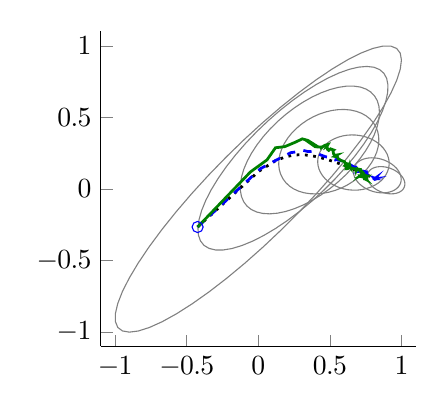
\begin{tikzpicture}

\begin{axis}[%
width=4cm,
height=4cm,
scale only axis,
xmin=-1.1,
xmax=1.1,
ymin=-1.1,
ymax=1.1,
axis x line*=bottom,
axis y line*=left
]
\addplot [
color=gray,
solid,
forget plot
]
table[row sep=crcr]{
-0.223606797749979 0.223606797749979\\
-0.0971317493977469 0.3464102286651\\
0.0309381995942439 0.463525613202567\\
0.15850014420423 0.573029919986106\\
0.283459520828355 0.67312509132574\\
0.403764499957141 0.762167567275353\\
0.517439677159302 0.838695272841565\\
0.6226185091679 0.9014516252147\\
0.717573962469178 0.949406166823786\\
0.800746871145116 0.981771485421374\\
0.870771538334692 0.998016143370882\\
0.926498160938592 0.997873403837886\\
0.967011709354304 0.98134561060157\\
0.991646952236901 0.948704149569941\\
0.999999379579327 0.900484992630715\\
0.991931844755535 0.837479897007744\\
0.967576816464294 0.760723404629287\\
0.927334203596814 0.671475854978151\\
0.871864788743812 0.571202690352226\\
0.80207937816364 0.461550393342469\\
0.719123846368702 0.344319451634276\\
0.624360320897642 0.221434794049475\\
0.519344816218816 0.0949141832682765\\
0.405801684015738 -0.0331649157781435\\
0.285595299380116 -0.16069944782438\\
0.16069944782438 -0.285595299380116\\
0.0331649157781437 -0.405801684015738\\
-0.0949141832682758 -0.519344816218815\\
-0.221434794049475 -0.624360320897642\\
-0.344319451634276 -0.719123846368702\\
-0.461550393342468 -0.80207937816364\\
-0.571202690352226 -0.871864788743812\\
-0.671475854978151 -0.927334203596814\\
-0.760723404629287 -0.967576816464294\\
-0.837479897007744 -0.991931844755535\\
-0.900484992630715 -0.999999379579327\\
-0.948704149569941 -0.991646952236901\\
-0.98134561060157 -0.967011709354304\\
-0.997873403837885 -0.926498160938592\\
-0.998016143370882 -0.870771538334693\\
-0.981771485421374 -0.800746871145116\\
-0.949406166823786 -0.717573962469179\\
-0.9014516252147 -0.6226185091679\\
-0.838695272841565 -0.517439677159303\\
-0.762167567275354 -0.403764499957142\\
-0.67312509132574 -0.283459520828355\\
-0.573029919986107 -0.15850014420423\\
-0.463525613202568 -0.030938199594244\\
-0.3464102286651 0.0971317493977463\\
-0.223606797749979 0.223606797749979\\
};
\addplot [
color=gray,
solid,
forget plot
]
table[row sep=crcr]{
0.456644734974626 -0.00969667801110813\\
0.374525791747298 -0.0847524663966239\\
0.29023584064942 -0.154897876594885\\
0.205158920347698 -0.218981122909709\\
0.120691991521408 -0.275949960208286\\
0.0382219988066626 -0.32486896175716\\
-0.0408969027961669 -0.364934878903337\\
-0.115365583110123 -0.395489830394961\\
-0.183961268463248 -0.416032104773275\\
-0.245557619598473 -0.426224398460909\\
-0.299143226133082 -0.425899354277293\\
-0.34383821388923 -0.415062309438937\\
-0.378908692403621 -0.39389120792248\\
-0.403778805388624 -0.362733678629514\\
-0.418040186276597 -0.322101327329635\\
-0.421458663587637 -0.272661336107845\\
-0.413978106018804 -0.215225508253162\\
-0.395721344118569 -0.150736938471062\\
-0.366988153412597 -0.0802545272944838\\
-0.32825033209791 -0.00493559396635573\\
-0.280143954129528 0.0739831267103794\\
-0.22345892490372 0.155205791524035\\
-0.159126011033233 0.237398726563892\\
-0.0882015571852386 0.319212326108943\\
-0.0118501409311103 0.399303213116517\\
0.0686745495851089 0.476356297436182\\
0.152050301171367 0.549106369553656\\
0.236908086291666 0.616358875296055\\
0.321854542460349 0.677009530378385\\
0.405494851215599 0.730062452720971\\
0.486455641000016 0.774646514805675\\
0.563407537883621 0.810029647565661\\
0.635086993847036 0.835630860939227\\
0.700317034205027 0.851029783710564\\
0.758026583498297 0.855973565993492\\
0.807268052522917 0.850381031019605\\
0.847232897718858 0.834344008058559\\
0.877264897432889 0.808125824584009\\
0.896870927059986 0.772156982443763\\
0.90572905613571 0.727028089031354\\
0.903693834425533 0.673480159528957\\
0.89079868021367 0.61239244945859\\
0.867255331575774 0.544768017330746\\
0.833450369645588 0.471717254451388\\
0.789938870963417 0.394439652327396\\
0.737435293134682 0.314204107049191\\
0.676801743455792 0.232328084052011\\
0.609033823136167 0.150155985369885\\
0.535244279553913 0.0690370745914021\\
0.456644734974626 -0.00969667801110799\\
};
\addplot [
color=gray,
solid,
forget plot
]
table[row sep=crcr]{
0.555425913311706 0.0472716755806835\\
0.496875664164754 -0.000161114180422195\\
0.436082271470401 -0.0431122116313219\\
0.374043961055967 -0.080876360939319\\
0.311779400263313 -0.112833475816823\\
0.250310971459259 -0.138458821321046\\
0.19064798454538 -0.157331629987261\\
0.133770104117331 -0.169142010818935\\
0.0806112633992654 -0.173696037689328\\
0.0320443290861189 -0.17091893360313\\
-0.011133231103392 -0.160856298532661\\
-0.0482124428246635 -0.14367336066758\\
-0.0785844664463428 -0.119652263372584\\
-0.101750594180242 -0.0891874324011575\\
-0.117330438849432 -0.0527790994356063\\
-0.125068179835172 -0.0110250882966617\\
-0.1248367636444 0.0353890013071266\\
-0.116639990124569 0.0857010513076516\\
-0.100612450070262 0.139084939234856\\
-0.0770173152460673 0.194664103124852\\
-0.0462420171134739 0.251525934643136\\
-0.00879188521699059 0.308736764088206\\
0.0347181503130071 0.365357191222255\\
0.0835736558960169 0.420457510197096\\
0.136972425481049 0.473132975298494\\
0.194037652747805 0.522518656845776\\
0.25383232824222 0.567803643313276\\
0.315374625045786 0.608244356475168\\
0.37765402034642 0.643176760939379\\
0.43964788819509 0.672027267590364\\
0.500338290995636 0.69432215190653\\
0.558728694011948 0.70969533250378\\
0.613860328440789 0.717894382181722\\
0.664827934369033 0.718784672771319\\
0.710794625116414 0.712351585725704\\
0.751005628891678 0.698700752156313\\
0.784800682124529 0.678056318372958\\
0.811624870975197 0.650757265407615\\
0.831037743004349 0.617251842955253\\
0.842720539389965 0.578090209126232\\
0.84648142893838 0.533915396865341\\
0.842258657947186 0.485452755368628\\
0.830121564199313 0.433498039869645\\
0.810269438438553 0.37890434536052\\
0.783028252021056 0.32256809879577\\
0.748845304474674 0.265414339786486\\
0.70828187885308 0.208381531475502\\
0.662004025483545 0.152406150998526\\
0.610771625438975 0.0984073125554682\\
0.555425913311706 0.0472716755806835\\
};
\addplot [
color=gray,
solid,
forget plot
]
table[row sep=crcr]{
0.622566809757817 0.028178664915152\\
0.57997101017793 0.00683114875754098\\
0.535938700569085 -0.0103515278383001\\
0.49119289023772 -0.0230872257977082\\
0.446468304152411 -0.0311668253122872\\
0.402499318780202 -0.0344576595813803\\
0.360007903645315 -0.0329056931972691\\
0.319691766609527 -0.0265364094050742\\
0.282212897528365 -0.0154543916685752\\
0.248186698395984 0.000158393587373684\\
0.218171878461432 0.0200455848605084\\
0.192661280238229 0.0438806350199351\\
0.172073787043923 0.0712721732009917\\
0.156747444947591 0.101770431104025\\
0.146933912062736 0.134874628177437\\
0.142794326328017 0.170041194420498\\
0.144396659626754 0.206692695787728\\
0.15171460169048 0.244227315639963\\
0.164627992112824 0.28202873655693\\
0.182924793380061 0.319476260252249\\
0.206304572521226 0.355954999422136\\
0.234383434209189 0.390865974177929\\
0.266700324311316 0.423635947279306\\
0.30272460038558 0.453726836673916\\
0.341864744814784 0.480644550789807\\
0.38347807750949 0.503947101505377\\
0.426881308697314 0.523251861582109\\
0.471361758522097 0.538241847393254\\
0.516189059227446 0.548670923786212\\
0.560627147775096 0.554367845614938\\
0.603946351979653 0.555239069580505\\
0.645435371705701 0.551270290209484\\
0.684412958396364 0.542526674749424\\
0.720239101155777 0.52915179312445\\
0.752325535710295 0.511365260521075\\
0.780145403691611 0.489459131312911\\
0.803241903636595 0.463793103535929\\
0.821235791654686 0.43478861265665\\
0.833831608602094 0.402921911613442\\
0.840822531512776 0.368716250756429\\
0.84209376962581 0.332733286091218\\
0.837624449246526 0.295563856902809\\
0.827487956491991 0.257818284190871\\
0.811850732292997 0.220116349215802\\
0.790969539438576 0.183077116707566\\
0.765187246538105 0.147308769839943\\
0.734927198128222 0.113398623879631\\
0.700686263367232 0.0819034824858006\\
0.663026677457268 0.0533404950094091\\
0.622566809757817 0.0281786649151521\\
};
\addplot [
color=gray,
solid,
forget plot
]
table[row sep=crcr]{
0.914082088679572 0.169354942779576\\
0.913540227303751 0.19408814269724\\
0.908912819009833 0.218665696555725\\
0.900275845714073 0.242684041600158\\
0.887771126279205 0.265748797268932\\
0.871603987852639 0.287481240911626\\
0.852039894400373 0.307524526404453\\
0.829400087796016 0.325549543553746\\
0.8040563130381 0.341260322076243\\
0.776424714207483 0.354398891422953\\
0.746959001393047 0.364749516648437\\
0.716143000784581 0.372142240772653\\
0.684482710260123 0.376455675469862\\
0.652497990914788 0.377618994261588\\
0.620714030955961 0.375613095485434\\
0.589652722127451 0.370470915943846\\
0.559824090261486 0.362276890082735\\
0.531717920668648 0.351165563580205\\
0.505795715876614 0.337319384110237\\
0.482483117771412 0.32096570555693\\
0.462162918569417 0.302373054870007\\
0.445168775379744 0.281846722859727\\
0.431779731563739 0.259723751330217\\
0.422215634850701 0.236367398862369\\
0.416633527444244 0.212161176117984\\
0.415125067393656 0.187502548605307\\
0.417715023571264 0.162796410306372\\
0.424360868968236 0.13844843532901\\
0.434953478986887 0.114858416749212\\
0.449318923263559 0.0924137020198785\\
0.467221321600384 0.0714828327363465\\
0.48836671711161 0.0524094931935867\\
0.512407902987538 0.0355068670995803\\
0.53895012362074 0.0210524951074926\\
0.567557556482218 0.00928371760582095\\
0.597760468315282 0.000393777595777522\\
0.629062928142637 -0.00547135235344862\\
0.660950950439322 -0.00821536697024131\\
0.692900934760816 -0.00779320961045532\\
0.724388263247867 -0.00421181208626706\\
0.75489591483723 0.00247001915398939\\
0.783922954733238 0.0121425686260781\\
0.810992759743295 0.0246470133350796\\
0.83566084441752 0.0397780306445759\\
0.857522159487549 0.0572871696686647\\
0.87621774276432 0.0768869308286371\\
0.891440613287296 0.0982554865881104\\
0.902940811943349 0.12104196585228\\
0.910529505788486 0.144872215261594\\
0.914082088679572 0.169354942779576\\
};
\addplot [
color=gray,
solid,
forget plot
]
table[row sep=crcr]{
0.795978184921688 -0.015786231265185\\
0.775374058911572 -0.00823025761854718\\
0.755687875383625 0.00102425255066693\\
0.737242880927121 0.0118253404413336\\
0.720341941841098 0.0239956524889001\\
0.705262571078097 0.0373353525060121\\
0.692252371489153 0.0516254029871843\\
0.681524970191831 0.0666311616985858\\
0.673256510818858 0.0821062344970318\\
0.667582761244544 0.0977965211150035\\
0.664596884280041 0.113444387480015\\
0.664347907942556 0.128792896058962\\
0.666839920416667 0.143590024765309\\
0.672032002926446 0.157592805154789\\
0.679838901620624 0.170571311960532\\
0.690132427438476 0.182312438459599\\
0.702743560970654 0.192623395679477\\
0.717465227753211 0.201334877987676\\
0.734055698424582 0.208303843085539\\
0.752242557915011 0.213415860758825\\
0.771727178494467 0.216586991818668\\
0.792189623231717 0.217765166380737\\
0.813293899349891 0.216931038851295\\
0.834693475218588 0.214098305581314\\
0.856036970393665 0.209313479972772\\
0.876973925274423 0.202655128729879\\
0.897160555640551 0.194232581795962\\
0.916265397579528 0.184184137158822\\
0.933974750114897 0.172674790001598\\
0.949997826167629 0.159893523486416\\
0.964071527271921 0.146050205656101\\
0.975964763644727 0.131372143406705\\
0.985482248673613 0.116100350114568\\
0.992467705517531 0.100485588203335\\
0.996806433168224 0.0847842516318938\\
0.998427189837622 0.0692541559126621\\
0.997303362746019 0.0541503047879964\\
0.99345340510319 0.0397207030757953\\
0.986940533107192 0.0262022844372453\\
0.977871687936142 0.0138170209326543\\
0.966395779777027 0.00276827824635879\\
0.952701242724551 -0.00676252357219119\\
0.937012940698509 -0.0146188890206284\\
0.919588475184443 -0.0206718167954904\\
0.900713955424368 -0.0248219179900562\\
0.880699300510929 -0.0270010480574468\\
0.859873150524472 -0.0271734257422009\\
0.838577470272004 -0.0253362206075004\\
0.817161934234519 -0.0215195995108649\\
0.795978184921688 -0.015786231265185\\
};
\addplot [
color=gray,
solid,
forget plot
]
table[row sep=crcr]{
1.0205476199241 0.0146304111508795\\
1.02334270847121 0.0256309088856638\\
1.02398659147348 0.037213622368035\\
1.02246869638982 0.0491883637628339\\
1.01881394701554 0.0613585081474175\\
1.01308235423431 0.0735242220874528\\
1.00536803064115 0.0854857448963837\\
0.995797645216192 0.0970466687003816\\
0.984528343423516 0.108017163450204\\
0.971745166887005 0.118217093925354\\
0.957658015011978 0.127478977549423\\
0.942498198442762 0.135650734449362\\
0.926514640948309 0.142598184602794\\
0.909969792100788 0.148207251070272\\
0.893135317860868 0.152385833135472\\
0.876287639830155 0.155065318596405\\
0.859703396416133 0.156201710375883\\
0.843654900437165 0.155776348952303\\
0.828405667753541 0.15379621874848\\
0.814206090344339 0.150293833447618\\
0.801289324878047 0.145326702119528\\
0.789867464286521 0.138976384923294\\
0.780128055204899 0.131347153891713\\
0.772231018461039 0.122564280787404\\
0.766306023179952 0.112771980143922\\
0.762450357620347 0.102131041267112\\
0.760727331704116 0.0908161880791451\\
0.761165237469171 0.0790132101565527\\
0.763756884514953 0.0669159120705125\\
0.768459718068622 0.0547229311211495\\
0.775196517733244 0.042634475718559\\
0.783856665444573 0.0308490379662483\\
0.794297961816613 0.0195601344262841\\
0.806348961051601 0.00895312858269419\\
0.819811786075265 -0.000797812821816249\\
0.834465377672916 -0.00953257959896436\\
0.850069124275642 -0.0171077471197552\\
0.866366812795615 -0.0233989313429241\\
0.883090835637911 -0.0283028311974558\\
0.89996658480982 -0.0317389247833146\\
0.916716960976494 -0.0336507915388166\\
0.933066923424366 -0.0340070386646928\\
0.94874800622206 -0.0328018165929853\\
0.963502726423567 -0.0300549150367915\\
0.977088811931092 -0.0258114380437218\\
0.98928317959621 -0.0201410633886851\\
0.999885598238992 -0.0131368984667513\\
1.00872197643844 -0.00491395147229781\\
1.01564722110882 0.00439275703236196\\
1.0205476199241 0.0146304111508795\\
};
\addplot [
color=blue,
only marks,
mark=o,
mark options={solid},
forget plot
]
table[row sep=crcr]{
-0.423658160306465 -0.265544277298046\\
};
\addplot [
color=black,
dotted,
line width=1.0pt,
forget plot
]
table[row sep=crcr]{
-0.423658160306465 -0.265544277298046\\
0.00242150590264467 0.122787079650492\\
0.119860995112355 0.196913937568555\\
0.188006844724955 0.22385638260482\\
0.237332543640276 0.234725527504476\\
0.276755147380961 0.238387931243253\\
0.309972822367975 0.238350330890813\\
0.33885921377211 0.236269678518997\\
0.364498667373003 0.233020943752307\\
0.387581375752828 0.22910191644929\\
0.408578923000339 0.224810830155441\\
0.427831457028349 0.220332911490062\\
0.445594872292462 0.215786008549946\\
0.462068175600546 0.211246163927359\\
0.477410287840286 0.206762662475913\\
0.491750864135096 0.202367241766044\\
0.505197550439098 0.198079914846599\\
0.517841022558555 0.193912751104659\\
0.52975859203918 0.189872386452409\\
0.541016854716125 0.185961720987173\\
0.551673680834573 0.18218108483713\\
0.561779740466219 0.178529048868203\\
0.571379693321013 0.175002994085654\\
0.58051313116453 0.171599514599526\\
0.589215334487547 0.16831470429785\\
0.597517887398241 0.165144361355447\\
0.605449182685881 0.162084134138763\\
0.613034840664175 0.159129624978834\\
0.620298059508905 0.156276463458587\\
0.627259910569584 0.153520357530856\\
0.633939589044394 0.150857128457993\\
0.640354628120062 0.148282733921915\\
0.646521082962575 0.145793282482559\\
0.652453689642047 0.143385041720243\\
0.658166003074998 0.141054441786378\\
0.663670517291457 0.138798075640508\\
0.668978770726548 0.136612696923383\\
0.674101438755884 0.13449521617294\\
0.679048415311284 0.132442695909547\\
0.683828885105843 0.130452344982138\\
0.688451387748645 0.128521512465838\\
0.692923874826822 0.126647681325779\\
0.697253760866618 0.124828462004642\\
0.70144796894823 0.123061586048288\\
0.705512971635701 0.121344899851306\\
0.709454827788602 0.119676358579702\\
0.713279215743047 0.118054020309453\\
0.716991463282974 0.116476040405716\\
0.720596574766369 0.114940666157084\\
0.724099255723382 0.113446231671519\\
0.727503935202617 0.111991153034902\\
0.73081478610719 0.110573923729004\\
0.734035743732302 0.109193110302682\\
0.737170522690515 0.107847348288089\\
0.740222632388734 0.106535338352286\\
0.743195391201804 0.105255842673812\\
0.746091939470981 0.104007681533272\\
0.748915251441087 0.102789730106862\\
0.751668146237511 0.101600915451779\\
0.754353297973212 0.100440213672642\\
0.756973245066157 0.0993066472583866\\
0.75953039883915 0.0981992825794537\\
0.762027051466476 0.0971172275355389\\
0.764465383325214 0.0960596293446205\\
0.766847469803174 0.0950256724644703\\
0.769175287610265 0.0940145766383234\\
0.771450720635486 0.0930255950568635\\
0.773675565387618 0.0920580126291417\\
0.775851536054101 0.0911111443554959\\
0.777980269209262 0.0901843337959739\\
0.780063328200204 0.0892769516281689\\
0.782102207236029 0.0883883942887737\\
0.784098335203756 0.0875180826935251\\
0.786053079232178 0.0866654610305641\\
0.787967748023034 0.0858299956225609\\
0.789843594967175 0.0850111738532671\\
0.791681821061853 0.0842085031544414\\
0.793483577643902 0.0834215100493708\\
0.795249968952332 0.0826497392494552\\
0.7969820545327 0.0818927528005651\\
0.798680851494636 0.0811501292760977\\
0.800347336632936 0.080421463013864\\
0.801982448421829 0.0797063633941279\\
0.803587088891209 0.0790044541562991\\
0.805162125392979 0.0783153727519431\\
0.806708392264973 0.0776387697319298\\
0.80822669239937 0.0769743081656825\\
0.809717798721966 0.0763216630906227\\
0.811182455588192 0.0756805209900316\\
0.812621380101344 0.0750505792976646\\
0.814035263358031 0.07443154592756\\
0.81542477162554 0.0738231388275862\\
0.816790547455432 0.0732250855553643\\
0.81813321073739 0.0726371228752879\\
0.819453359697028 0.0720589963754441\\
0.820751571841154 0.0714904601033156\\
0.822028404853678 0.070931276219213\\
0.823284397445168 0.0703812146664506\\
0.824520070158853 0.0698400528573428\\
0.825735926135646 0.0693075753741537\\
0.826932451840631 0.0687835736841832\\
};
\addplot [
color=blue,
dashed,
line width=1.0pt,
forget plot
]
table[row sep=crcr]{
-0.423658160306465 -0.265544277298046\\
0.0150764734847799 0.141713645028666\\
0.128266448251792 0.203061419228372\\
0.22669657170916 0.253535394239362\\
0.276984522465355 0.261006022043223\\
0.314160741859687 0.269650622899764\\
0.347821518442704 0.261207424958875\\
0.378195026465508 0.262517933514043\\
0.403124906907465 0.25388294243401\\
0.418451275881427 0.244472637319418\\
0.439771613306922 0.236075699622215\\
0.457446033461072 0.229817673462225\\
0.470032041223307 0.224368357039128\\
0.491317179742705 0.223780708510906\\
0.500003115472698 0.214399545231926\\
0.510240222954932 0.210945973885522\\
0.518283740368447 0.206410615746778\\
0.537532706535306 0.202242328096033\\
0.544284701549024 0.205948198993329\\
0.554302655300813 0.204588987811089\\
0.558552231168685 0.202072651240517\\
0.574335222619425 0.198786965164456\\
0.580249746446143 0.197109623497662\\
0.590174871682169 0.189637286960168\\
0.601160310406428 0.193743972514359\\
0.609171759818325 0.184341134243007\\
0.620281677824765 0.178174882673582\\
0.628884799103075 0.173126404023472\\
0.642402014841729 0.169133561500065\\
0.654311318750228 0.162843724927911\\
0.666329303265718 0.154246854556376\\
0.682765042033113 0.153180031510408\\
0.686800080206799 0.149885830747641\\
0.695221437779026 0.141711532082627\\
0.694804262768244 0.141000393817934\\
0.695013585666167 0.141902583100789\\
0.700129999401421 0.138936953160248\\
0.702333756902603 0.134448150740603\\
0.700009325319683 0.135249005050468\\
0.704666564242927 0.131218554528193\\
0.706390968286814 0.132734911121016\\
0.709946020328424 0.128802249694482\\
0.719419507674847 0.127246315289755\\
0.722642272155939 0.127345774869413\\
0.721809839856199 0.126715450299851\\
0.725148241023072 0.125431226578078\\
0.724449245144119 0.125139770483216\\
0.729507139516062 0.125706382584547\\
0.735055750532655 0.123736664050632\\
0.737503370711441 0.122274940478969\\
0.745300490304115 0.121349546245666\\
0.749295460965084 0.117506133931847\\
0.752634599553002 0.117132929282051\\
0.755183319264509 0.115425050709325\\
0.755655853464857 0.113227657699763\\
0.758028539676943 0.111343587244499\\
0.757295116784256 0.113715590494597\\
0.755826792170151 0.111888078748728\\
0.757662841985657 0.111615130214658\\
0.757822207564221 0.109098462894216\\
0.761292304123277 0.10167333198567\\
0.760586903991302 0.102740448720043\\
0.764023718942325 0.0984064214066678\\
0.766719011053783 0.0973923522181611\\
0.76961536445881 0.0971315362800118\\
0.778073805626339 0.0910693389405452\\
0.783473762085921 0.0865437273795604\\
0.787238214973759 0.0822323217366929\\
0.789343424791777 0.08259015816049\\
0.794259185396647 0.0801776890521058\\
0.792512714679819 0.081463090579629\\
0.796719722610988 0.0814962705039133\\
0.801003635406211 0.0808568021145043\\
0.806411873120944 0.0766775287254546\\
0.810618242255894 0.0772197090558023\\
0.805839159499941 0.0782065097389542\\
0.808065627761535 0.0756642096008819\\
0.812156222221671 0.0734156369277934\\
0.815770119780439 0.0734435499205703\\
0.816756666417879 0.0745972461736448\\
0.815294717032733 0.0735464680265237\\
0.814494774658996 0.0722875185100304\\
0.816703929578228 0.0722415452207195\\
0.812692778557632 0.0741879839787607\\
0.814002603911476 0.0710724194508479\\
0.820501093627315 0.0718321762859395\\
0.818647899243582 0.0711293118976905\\
0.819011976553334 0.0733112266091904\\
0.82200990231907 0.0726475207041034\\
0.82202669626064 0.0691426478181728\\
0.82349899646827 0.0694836750869472\\
0.823783637607849 0.0688108694594397\\
0.826880909090058 0.0685441765496974\\
0.827545452125074 0.0679062463922276\\
0.826943669030874 0.0674114110356461\\
0.82745608819192 0.0675230320209754\\
0.834046637327064 0.0679194615839197\\
0.832375493903718 0.0707538789032289\\
0.831490871272005 0.0709659999278264\\
0.831660602192682 0.0689006934969698\\
0.828829415415717 0.0698164321398679\\
};
\addplot [
color=green!50!black,
solid,
line width=1.0pt,
forget plot
]
table[row sep=crcr]{
-0.423658160306465 -0.265544277298046\\
-0.0549619814773591 0.118905560965915\\
0.0611900825861636 0.203436753119323\\
0.120109030303461 0.287894077984681\\
0.184914785888709 0.295752039420244\\
0.258056733824465 0.32631445172747\\
0.307562099907215 0.350034232288437\\
0.346474534696256 0.339153890567492\\
0.383539193743067 0.315737286050682\\
0.355931520963756 0.324350689858913\\
0.397483596186667 0.295193766511885\\
0.42160539285663 0.292692105062653\\
0.436539752075579 0.293636432715814\\
0.439240287549775 0.28734870752013\\
0.45483391205266 0.299050655909251\\
0.465827688634448 0.305178168644249\\
0.487123661934733 0.310835883476853\\
0.478326164058298 0.295864544264346\\
0.48179786392265 0.29777218887497\\
0.483240802146808 0.277043008568191\\
0.49222239974003 0.269592894710355\\
0.505132748333046 0.280406737967897\\
0.526241657930929 0.272337269125332\\
0.521063838650468 0.268730671114344\\
0.521929060573914 0.26595276421186\\
0.526455207115231 0.24452964915957\\
0.536813902515015 0.235196942231384\\
0.550790212208966 0.237689137012003\\
0.533795508169064 0.227429084719918\\
0.553130903549037 0.22426921659041\\
0.559228100048614 0.210245915387877\\
0.583184021124399 0.196892370434251\\
0.602789764235752 0.190688210814037\\
0.605910075020372 0.181043904535424\\
0.615367888791609 0.178347559098766\\
0.625524290857247 0.172944316175946\\
0.61252301838854 0.169359695785367\\
0.606335949811397 0.163513821824845\\
0.617714299649339 0.160639287931992\\
0.634139790657078 0.156547337341809\\
0.637526304424482 0.149979800156245\\
0.629034318689475 0.168177836518465\\
0.621918753545596 0.160401808334733\\
0.615350304501684 0.14191045391587\\
0.623998664699659 0.14312609088017\\
0.623413471042154 0.148054993164301\\
0.620078683167653 0.144487005575743\\
0.612786167829917 0.152775245792342\\
0.615782667214696 0.149574545211305\\
0.620183039053663 0.153644365832568\\
0.622117976017808 0.156453812622943\\
0.635256479971316 0.156014726760737\\
0.642712610390725 0.147535027230091\\
0.640339563568981 0.157877258361172\\
0.638736857164934 0.148794419678204\\
0.657020679494355 0.1441900339601\\
0.672262214796502 0.140033157968078\\
0.674158209282595 0.140499702518238\\
0.682265172645078 0.130439010286057\\
0.68136474498082 0.127410439357832\\
0.679543455406662 0.134539893519713\\
0.685954363558128 0.13267623202126\\
0.686999377926314 0.141661895787656\\
0.683750391259635 0.140709003931584\\
0.683837737346897 0.138175699198264\\
0.705805494997607 0.137005164528778\\
0.703856483125101 0.134476368547535\\
0.711762564385371 0.125299162432966\\
0.716320152850343 0.130460221181414\\
0.721973251206943 0.123262838037093\\
0.724617414621529 0.121780762986902\\
0.728972169917787 0.127867252699477\\
0.726321971162613 0.123417117163446\\
0.730291169468817 0.110756619933168\\
0.732778540569512 0.109336727810331\\
0.71939922351489 0.09666849140913\\
0.724571867219492 0.0993930159422993\\
0.7304649705255 0.0987085850835294\\
0.74004773871398 0.0963032494376266\\
0.725864838562941 0.0944192197513796\\
0.732554899407043 0.0977490672468534\\
0.736100629131383 0.0951499722647115\\
0.731167153556259 0.0941590842633866\\
0.729505787845459 0.0871793520300228\\
0.732001511005409 0.0833510725177911\\
0.714569519023427 0.0872609151851703\\
0.717406851231904 0.0905376992739934\\
0.715648115959882 0.0920291538214647\\
0.724208891560132 0.0923151040681435\\
0.740820704133793 0.0867245380769161\\
0.744416546861374 0.0810664401026933\\
0.758115927612689 0.0745443682255588\\
0.759110081304389 0.0685067070430162\\
0.749894291964036 0.0702345639255953\\
0.754982717939339 0.0646159279017507\\
0.742460324108607 0.0711199205373331\\
0.741651052874918 0.0730930395131353\\
0.749651747703426 0.0758540715647245\\
0.747658963283614 0.0741493804225888\\
0.743074704301771 0.0732882500238929\\
0.743427204107473 0.0764487169924193\\
};
\end{axis}
\end{tikzpicture}% }
\subfloat[]{ % This file was created by matlab2tikz v0.4.4 running on MATLAB 7.13.
% Copyright (c) 2008--2013, Nico Schlömer <nico.schloemer@gmail.com>
% All rights reserved.
% 
% The latest updates can be retrieved from
%   http://www.mathworks.com/matlabcentral/fileexchange/22022-matlab2tikz
% where you can also make suggestions and rate matlab2tikz.
% 
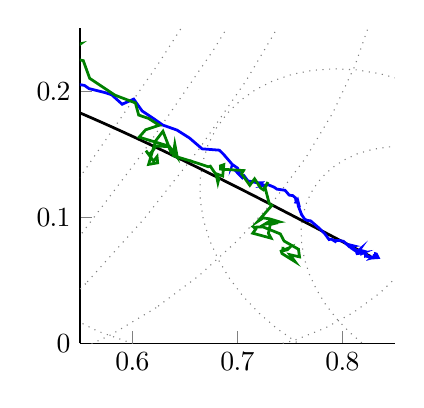
\begin{tikzpicture}

\begin{axis}[%
width=4cm,
height=4cm,
scale only axis,
xmin=0.55,
xmax=0.85,
ymin=0,
ymax=0.25,
axis x line*=bottom,
axis y line*=left
]
\addplot [
color=gray,
dotted,
forget plot
]
table[row sep=crcr]{
-0.223606797749979 0.223606797749979\\
-0.0971317493977469 0.3464102286651\\
0.0309381995942439 0.463525613202567\\
0.15850014420423 0.573029919986106\\
0.283459520828355 0.67312509132574\\
0.403764499957141 0.762167567275353\\
0.517439677159302 0.838695272841565\\
0.6226185091679 0.9014516252147\\
0.717573962469178 0.949406166823786\\
0.800746871145116 0.981771485421374\\
0.870771538334692 0.998016143370882\\
0.926498160938592 0.997873403837886\\
0.967011709354304 0.98134561060157\\
0.991646952236901 0.948704149569941\\
0.999999379579327 0.900484992630715\\
0.991931844755535 0.837479897007744\\
0.967576816464294 0.760723404629287\\
0.927334203596814 0.671475854978151\\
0.871864788743812 0.571202690352226\\
0.80207937816364 0.461550393342469\\
0.719123846368702 0.344319451634276\\
0.624360320897642 0.221434794049475\\
0.519344816218816 0.0949141832682765\\
0.405801684015738 -0.0331649157781435\\
0.285595299380116 -0.16069944782438\\
0.16069944782438 -0.285595299380116\\
0.0331649157781437 -0.405801684015738\\
-0.0949141832682758 -0.519344816218815\\
-0.221434794049475 -0.624360320897642\\
-0.344319451634276 -0.719123846368702\\
-0.461550393342468 -0.80207937816364\\
-0.571202690352226 -0.871864788743812\\
-0.671475854978151 -0.927334203596814\\
-0.760723404629287 -0.967576816464294\\
-0.837479897007744 -0.991931844755535\\
-0.900484992630715 -0.999999379579327\\
-0.948704149569941 -0.991646952236901\\
-0.98134561060157 -0.967011709354304\\
-0.997873403837885 -0.926498160938592\\
-0.998016143370882 -0.870771538334693\\
-0.981771485421374 -0.800746871145116\\
-0.949406166823786 -0.717573962469179\\
-0.9014516252147 -0.6226185091679\\
-0.838695272841565 -0.517439677159303\\
-0.762167567275354 -0.403764499957142\\
-0.67312509132574 -0.283459520828355\\
-0.573029919986107 -0.15850014420423\\
-0.463525613202568 -0.030938199594244\\
-0.3464102286651 0.0971317493977463\\
-0.223606797749979 0.223606797749979\\
};
\addplot [
color=gray,
dotted,
forget plot
]
table[row sep=crcr]{
0.456644734974626 -0.00969667801110813\\
0.374525791747298 -0.0847524663966239\\
0.29023584064942 -0.154897876594885\\
0.205158920347698 -0.218981122909709\\
0.120691991521408 -0.275949960208286\\
0.0382219988066626 -0.32486896175716\\
-0.0408969027961669 -0.364934878903337\\
-0.115365583110123 -0.395489830394961\\
-0.183961268463248 -0.416032104773275\\
-0.245557619598473 -0.426224398460909\\
-0.299143226133082 -0.425899354277293\\
-0.34383821388923 -0.415062309438937\\
-0.378908692403621 -0.39389120792248\\
-0.403778805388624 -0.362733678629514\\
-0.418040186276597 -0.322101327329635\\
-0.421458663587637 -0.272661336107845\\
-0.413978106018804 -0.215225508253162\\
-0.395721344118569 -0.150736938471062\\
-0.366988153412597 -0.0802545272944838\\
-0.32825033209791 -0.00493559396635573\\
-0.280143954129528 0.0739831267103794\\
-0.22345892490372 0.155205791524035\\
-0.159126011033233 0.237398726563892\\
-0.0882015571852386 0.319212326108943\\
-0.0118501409311103 0.399303213116517\\
0.0686745495851089 0.476356297436182\\
0.152050301171367 0.549106369553656\\
0.236908086291666 0.616358875296055\\
0.321854542460349 0.677009530378385\\
0.405494851215599 0.730062452720971\\
0.486455641000016 0.774646514805675\\
0.563407537883621 0.810029647565661\\
0.635086993847036 0.835630860939227\\
0.700317034205027 0.851029783710564\\
0.758026583498297 0.855973565993492\\
0.807268052522917 0.850381031019605\\
0.847232897718858 0.834344008058559\\
0.877264897432889 0.808125824584009\\
0.896870927059986 0.772156982443763\\
0.90572905613571 0.727028089031354\\
0.903693834425533 0.673480159528957\\
0.89079868021367 0.61239244945859\\
0.867255331575774 0.544768017330746\\
0.833450369645588 0.471717254451388\\
0.789938870963417 0.394439652327396\\
0.737435293134682 0.314204107049191\\
0.676801743455792 0.232328084052011\\
0.609033823136167 0.150155985369885\\
0.535244279553913 0.0690370745914021\\
0.456644734974626 -0.00969667801110799\\
};
\addplot [
color=gray,
dotted,
forget plot
]
table[row sep=crcr]{
0.555425913311706 0.0472716755806835\\
0.496875664164754 -0.000161114180422195\\
0.436082271470401 -0.0431122116313219\\
0.374043961055967 -0.080876360939319\\
0.311779400263313 -0.112833475816823\\
0.250310971459259 -0.138458821321046\\
0.19064798454538 -0.157331629987261\\
0.133770104117331 -0.169142010818935\\
0.0806112633992654 -0.173696037689328\\
0.0320443290861189 -0.17091893360313\\
-0.011133231103392 -0.160856298532661\\
-0.0482124428246635 -0.14367336066758\\
-0.0785844664463428 -0.119652263372584\\
-0.101750594180242 -0.0891874324011575\\
-0.117330438849432 -0.0527790994356063\\
-0.125068179835172 -0.0110250882966617\\
-0.1248367636444 0.0353890013071266\\
-0.116639990124569 0.0857010513076516\\
-0.100612450070262 0.139084939234856\\
-0.0770173152460673 0.194664103124852\\
-0.0462420171134739 0.251525934643136\\
-0.00879188521699059 0.308736764088206\\
0.0347181503130071 0.365357191222255\\
0.0835736558960169 0.420457510197096\\
0.136972425481049 0.473132975298494\\
0.194037652747805 0.522518656845776\\
0.25383232824222 0.567803643313276\\
0.315374625045786 0.608244356475168\\
0.37765402034642 0.643176760939379\\
0.43964788819509 0.672027267590364\\
0.500338290995636 0.69432215190653\\
0.558728694011948 0.70969533250378\\
0.613860328440789 0.717894382181722\\
0.664827934369033 0.718784672771319\\
0.710794625116414 0.712351585725704\\
0.751005628891678 0.698700752156313\\
0.784800682124529 0.678056318372958\\
0.811624870975197 0.650757265407615\\
0.831037743004349 0.617251842955253\\
0.842720539389965 0.578090209126232\\
0.84648142893838 0.533915396865341\\
0.842258657947186 0.485452755368628\\
0.830121564199313 0.433498039869645\\
0.810269438438553 0.37890434536052\\
0.783028252021056 0.32256809879577\\
0.748845304474674 0.265414339786486\\
0.70828187885308 0.208381531475502\\
0.662004025483545 0.152406150998526\\
0.610771625438975 0.0984073125554682\\
0.555425913311706 0.0472716755806835\\
};
\addplot [
color=gray,
dotted,
forget plot
]
table[row sep=crcr]{
0.622566809757817 0.028178664915152\\
0.57997101017793 0.00683114875754098\\
0.535938700569085 -0.0103515278383001\\
0.49119289023772 -0.0230872257977082\\
0.446468304152411 -0.0311668253122872\\
0.402499318780202 -0.0344576595813803\\
0.360007903645315 -0.0329056931972691\\
0.319691766609527 -0.0265364094050742\\
0.282212897528365 -0.0154543916685752\\
0.248186698395984 0.000158393587373684\\
0.218171878461432 0.0200455848605084\\
0.192661280238229 0.0438806350199351\\
0.172073787043923 0.0712721732009917\\
0.156747444947591 0.101770431104025\\
0.146933912062736 0.134874628177437\\
0.142794326328017 0.170041194420498\\
0.144396659626754 0.206692695787728\\
0.15171460169048 0.244227315639963\\
0.164627992112824 0.28202873655693\\
0.182924793380061 0.319476260252249\\
0.206304572521226 0.355954999422136\\
0.234383434209189 0.390865974177929\\
0.266700324311316 0.423635947279306\\
0.30272460038558 0.453726836673916\\
0.341864744814784 0.480644550789807\\
0.38347807750949 0.503947101505377\\
0.426881308697314 0.523251861582109\\
0.471361758522097 0.538241847393254\\
0.516189059227446 0.548670923786212\\
0.560627147775096 0.554367845614938\\
0.603946351979653 0.555239069580505\\
0.645435371705701 0.551270290209484\\
0.684412958396364 0.542526674749424\\
0.720239101155777 0.52915179312445\\
0.752325535710295 0.511365260521075\\
0.780145403691611 0.489459131312911\\
0.803241903636595 0.463793103535929\\
0.821235791654686 0.43478861265665\\
0.833831608602094 0.402921911613442\\
0.840822531512776 0.368716250756429\\
0.84209376962581 0.332733286091218\\
0.837624449246526 0.295563856902809\\
0.827487956491991 0.257818284190871\\
0.811850732292997 0.220116349215802\\
0.790969539438576 0.183077116707566\\
0.765187246538105 0.147308769839943\\
0.734927198128222 0.113398623879631\\
0.700686263367232 0.0819034824858006\\
0.663026677457268 0.0533404950094091\\
0.622566809757817 0.0281786649151521\\
};
\addplot [
color=gray,
dotted,
forget plot
]
table[row sep=crcr]{
0.914082088679572 0.169354942779576\\
0.913540227303751 0.19408814269724\\
0.908912819009833 0.218665696555725\\
0.900275845714073 0.242684041600158\\
0.887771126279205 0.265748797268932\\
0.871603987852639 0.287481240911626\\
0.852039894400373 0.307524526404453\\
0.829400087796016 0.325549543553746\\
0.8040563130381 0.341260322076243\\
0.776424714207483 0.354398891422953\\
0.746959001393047 0.364749516648437\\
0.716143000784581 0.372142240772653\\
0.684482710260123 0.376455675469862\\
0.652497990914788 0.377618994261588\\
0.620714030955961 0.375613095485434\\
0.589652722127451 0.370470915943846\\
0.559824090261486 0.362276890082735\\
0.531717920668648 0.351165563580205\\
0.505795715876614 0.337319384110237\\
0.482483117771412 0.32096570555693\\
0.462162918569417 0.302373054870007\\
0.445168775379744 0.281846722859727\\
0.431779731563739 0.259723751330217\\
0.422215634850701 0.236367398862369\\
0.416633527444244 0.212161176117984\\
0.415125067393656 0.187502548605307\\
0.417715023571264 0.162796410306372\\
0.424360868968236 0.13844843532901\\
0.434953478986887 0.114858416749212\\
0.449318923263559 0.0924137020198785\\
0.467221321600384 0.0714828327363465\\
0.48836671711161 0.0524094931935867\\
0.512407902987538 0.0355068670995803\\
0.53895012362074 0.0210524951074926\\
0.567557556482218 0.00928371760582095\\
0.597760468315282 0.000393777595777522\\
0.629062928142637 -0.00547135235344862\\
0.660950950439322 -0.00821536697024131\\
0.692900934760816 -0.00779320961045532\\
0.724388263247867 -0.00421181208626706\\
0.75489591483723 0.00247001915398939\\
0.783922954733238 0.0121425686260781\\
0.810992759743295 0.0246470133350796\\
0.83566084441752 0.0397780306445759\\
0.857522159487549 0.0572871696686647\\
0.87621774276432 0.0768869308286371\\
0.891440613287296 0.0982554865881104\\
0.902940811943349 0.12104196585228\\
0.910529505788486 0.144872215261594\\
0.914082088679572 0.169354942779576\\
};
\addplot [
color=gray,
dotted,
forget plot
]
table[row sep=crcr]{
0.795978184921688 -0.015786231265185\\
0.775374058911572 -0.00823025761854718\\
0.755687875383625 0.00102425255066693\\
0.737242880927121 0.0118253404413336\\
0.720341941841098 0.0239956524889001\\
0.705262571078097 0.0373353525060121\\
0.692252371489153 0.0516254029871843\\
0.681524970191831 0.0666311616985858\\
0.673256510818858 0.0821062344970318\\
0.667582761244544 0.0977965211150035\\
0.664596884280041 0.113444387480015\\
0.664347907942556 0.128792896058962\\
0.666839920416667 0.143590024765309\\
0.672032002926446 0.157592805154789\\
0.679838901620624 0.170571311960532\\
0.690132427438476 0.182312438459599\\
0.702743560970654 0.192623395679477\\
0.717465227753211 0.201334877987676\\
0.734055698424582 0.208303843085539\\
0.752242557915011 0.213415860758825\\
0.771727178494467 0.216586991818668\\
0.792189623231717 0.217765166380737\\
0.813293899349891 0.216931038851295\\
0.834693475218588 0.214098305581314\\
0.856036970393665 0.209313479972772\\
0.876973925274423 0.202655128729879\\
0.897160555640551 0.194232581795962\\
0.916265397579528 0.184184137158822\\
0.933974750114897 0.172674790001598\\
0.949997826167629 0.159893523486416\\
0.964071527271921 0.146050205656101\\
0.975964763644727 0.131372143406705\\
0.985482248673613 0.116100350114568\\
0.992467705517531 0.100485588203335\\
0.996806433168224 0.0847842516318938\\
0.998427189837622 0.0692541559126621\\
0.997303362746019 0.0541503047879964\\
0.99345340510319 0.0397207030757953\\
0.986940533107192 0.0262022844372453\\
0.977871687936142 0.0138170209326543\\
0.966395779777027 0.00276827824635879\\
0.952701242724551 -0.00676252357219119\\
0.937012940698509 -0.0146188890206284\\
0.919588475184443 -0.0206718167954904\\
0.900713955424368 -0.0248219179900562\\
0.880699300510929 -0.0270010480574468\\
0.859873150524472 -0.0271734257422009\\
0.838577470272004 -0.0253362206075004\\
0.817161934234519 -0.0215195995108649\\
0.795978184921688 -0.015786231265185\\
};
\addplot [
color=gray,
dotted,
forget plot
]
table[row sep=crcr]{
1.0205476199241 0.0146304111508795\\
1.02334270847121 0.0256309088856638\\
1.02398659147348 0.037213622368035\\
1.02246869638982 0.0491883637628339\\
1.01881394701554 0.0613585081474175\\
1.01308235423431 0.0735242220874528\\
1.00536803064115 0.0854857448963837\\
0.995797645216192 0.0970466687003816\\
0.984528343423516 0.108017163450204\\
0.971745166887005 0.118217093925354\\
0.957658015011978 0.127478977549423\\
0.942498198442762 0.135650734449362\\
0.926514640948309 0.142598184602794\\
0.909969792100788 0.148207251070272\\
0.893135317860868 0.152385833135472\\
0.876287639830155 0.155065318596405\\
0.859703396416133 0.156201710375883\\
0.843654900437165 0.155776348952303\\
0.828405667753541 0.15379621874848\\
0.814206090344339 0.150293833447618\\
0.801289324878047 0.145326702119528\\
0.789867464286521 0.138976384923294\\
0.780128055204899 0.131347153891713\\
0.772231018461039 0.122564280787404\\
0.766306023179952 0.112771980143922\\
0.762450357620347 0.102131041267112\\
0.760727331704116 0.0908161880791451\\
0.761165237469171 0.0790132101565527\\
0.763756884514953 0.0669159120705125\\
0.768459718068622 0.0547229311211495\\
0.775196517733244 0.042634475718559\\
0.783856665444573 0.0308490379662483\\
0.794297961816613 0.0195601344262841\\
0.806348961051601 0.00895312858269419\\
0.819811786075265 -0.000797812821816249\\
0.834465377672916 -0.00953257959896436\\
0.850069124275642 -0.0171077471197552\\
0.866366812795615 -0.0233989313429241\\
0.883090835637911 -0.0283028311974558\\
0.89996658480982 -0.0317389247833146\\
0.916716960976494 -0.0336507915388166\\
0.933066923424366 -0.0340070386646928\\
0.94874800622206 -0.0328018165929853\\
0.963502726423567 -0.0300549150367915\\
0.977088811931092 -0.0258114380437218\\
0.98928317959621 -0.0201410633886851\\
0.999885598238992 -0.0131368984667513\\
1.00872197643844 -0.00491395147229781\\
1.01564722110882 0.00439275703236196\\
1.0205476199241 0.0146304111508795\\
};
\addplot [
color=black,
solid,
line width=1.0pt,
forget plot
]
table[row sep=crcr]{
-0.423658160306465 -0.265544277298046\\
0.00242150590264467 0.122787079650492\\
0.119860995112355 0.196913937568555\\
0.188006844724955 0.22385638260482\\
0.237332543640276 0.234725527504476\\
0.276755147380961 0.238387931243253\\
0.309972822367975 0.238350330890813\\
0.33885921377211 0.236269678518997\\
0.364498667373003 0.233020943752307\\
0.387581375752828 0.22910191644929\\
0.408578923000339 0.224810830155441\\
0.427831457028349 0.220332911490062\\
0.445594872292462 0.215786008549946\\
0.462068175600546 0.211246163927359\\
0.477410287840286 0.206762662475913\\
0.491750864135096 0.202367241766044\\
0.505197550439098 0.198079914846599\\
0.517841022558555 0.193912751104659\\
0.52975859203918 0.189872386452409\\
0.541016854716125 0.185961720987173\\
0.551673680834573 0.18218108483713\\
0.561779740466219 0.178529048868203\\
0.571379693321013 0.175002994085654\\
0.58051313116453 0.171599514599526\\
0.589215334487547 0.16831470429785\\
0.597517887398241 0.165144361355447\\
0.605449182685881 0.162084134138763\\
0.613034840664175 0.159129624978834\\
0.620298059508905 0.156276463458587\\
0.627259910569584 0.153520357530856\\
0.633939589044394 0.150857128457993\\
0.640354628120062 0.148282733921915\\
0.646521082962575 0.145793282482559\\
0.652453689642047 0.143385041720243\\
0.658166003074998 0.141054441786378\\
0.663670517291457 0.138798075640508\\
0.668978770726548 0.136612696923383\\
0.674101438755884 0.13449521617294\\
0.679048415311284 0.132442695909547\\
0.683828885105843 0.130452344982138\\
0.688451387748645 0.128521512465838\\
0.692923874826822 0.126647681325779\\
0.697253760866618 0.124828462004642\\
0.70144796894823 0.123061586048288\\
0.705512971635701 0.121344899851306\\
0.709454827788602 0.119676358579702\\
0.713279215743047 0.118054020309453\\
0.716991463282974 0.116476040405716\\
0.720596574766369 0.114940666157084\\
0.724099255723382 0.113446231671519\\
0.727503935202617 0.111991153034902\\
0.73081478610719 0.110573923729004\\
0.734035743732302 0.109193110302682\\
0.737170522690515 0.107847348288089\\
0.740222632388734 0.106535338352286\\
0.743195391201804 0.105255842673812\\
0.746091939470981 0.104007681533272\\
0.748915251441087 0.102789730106862\\
0.751668146237511 0.101600915451779\\
0.754353297973212 0.100440213672642\\
0.756973245066157 0.0993066472583866\\
0.75953039883915 0.0981992825794537\\
0.762027051466476 0.0971172275355389\\
0.764465383325214 0.0960596293446205\\
0.766847469803174 0.0950256724644703\\
0.769175287610265 0.0940145766383234\\
0.771450720635486 0.0930255950568635\\
0.773675565387618 0.0920580126291417\\
0.775851536054101 0.0911111443554959\\
0.777980269209262 0.0901843337959739\\
0.780063328200204 0.0892769516281689\\
0.782102207236029 0.0883883942887737\\
0.784098335203756 0.0875180826935251\\
0.786053079232178 0.0866654610305641\\
0.787967748023034 0.0858299956225609\\
0.789843594967175 0.0850111738532671\\
0.791681821061853 0.0842085031544414\\
0.793483577643902 0.0834215100493708\\
0.795249968952332 0.0826497392494552\\
0.7969820545327 0.0818927528005651\\
0.798680851494636 0.0811501292760977\\
0.800347336632936 0.080421463013864\\
0.801982448421829 0.0797063633941279\\
0.803587088891209 0.0790044541562991\\
0.805162125392979 0.0783153727519431\\
0.806708392264973 0.0776387697319298\\
0.80822669239937 0.0769743081656825\\
0.809717798721966 0.0763216630906227\\
0.811182455588192 0.0756805209900316\\
0.812621380101344 0.0750505792976646\\
0.814035263358031 0.07443154592756\\
0.81542477162554 0.0738231388275862\\
0.816790547455432 0.0732250855553643\\
0.81813321073739 0.0726371228752879\\
0.819453359697028 0.0720589963754441\\
0.820751571841154 0.0714904601033156\\
0.822028404853678 0.070931276219213\\
0.823284397445168 0.0703812146664506\\
0.824520070158853 0.0698400528573428\\
0.825735926135646 0.0693075753741537\\
0.826932451840631 0.0687835736841832\\
};
\addplot [
color=blue,
solid,
line width=1.0pt,
forget plot
]
table[row sep=crcr]{
-0.423658160306465 -0.265544277298046\\
0.0150764734847799 0.141713645028666\\
0.128266448251792 0.203061419228372\\
0.22669657170916 0.253535394239362\\
0.276984522465355 0.261006022043223\\
0.314160741859687 0.269650622899764\\
0.347821518442704 0.261207424958875\\
0.378195026465508 0.262517933514043\\
0.403124906907465 0.25388294243401\\
0.418451275881427 0.244472637319418\\
0.439771613306922 0.236075699622215\\
0.457446033461072 0.229817673462225\\
0.470032041223307 0.224368357039128\\
0.491317179742705 0.223780708510906\\
0.500003115472698 0.214399545231926\\
0.510240222954932 0.210945973885522\\
0.518283740368447 0.206410615746778\\
0.537532706535306 0.202242328096033\\
0.544284701549024 0.205948198993329\\
0.554302655300813 0.204588987811089\\
0.558552231168685 0.202072651240517\\
0.574335222619425 0.198786965164456\\
0.580249746446143 0.197109623497662\\
0.590174871682169 0.189637286960168\\
0.601160310406428 0.193743972514359\\
0.609171759818325 0.184341134243007\\
0.620281677824765 0.178174882673582\\
0.628884799103075 0.173126404023472\\
0.642402014841729 0.169133561500065\\
0.654311318750228 0.162843724927911\\
0.666329303265718 0.154246854556376\\
0.682765042033113 0.153180031510408\\
0.686800080206799 0.149885830747641\\
0.695221437779026 0.141711532082627\\
0.694804262768244 0.141000393817934\\
0.695013585666167 0.141902583100789\\
0.700129999401421 0.138936953160248\\
0.702333756902603 0.134448150740603\\
0.700009325319683 0.135249005050468\\
0.704666564242927 0.131218554528193\\
0.706390968286814 0.132734911121016\\
0.709946020328424 0.128802249694482\\
0.719419507674847 0.127246315289755\\
0.722642272155939 0.127345774869413\\
0.721809839856199 0.126715450299851\\
0.725148241023072 0.125431226578078\\
0.724449245144119 0.125139770483216\\
0.729507139516062 0.125706382584547\\
0.735055750532655 0.123736664050632\\
0.737503370711441 0.122274940478969\\
0.745300490304115 0.121349546245666\\
0.749295460965084 0.117506133931847\\
0.752634599553002 0.117132929282051\\
0.755183319264509 0.115425050709325\\
0.755655853464857 0.113227657699763\\
0.758028539676943 0.111343587244499\\
0.757295116784256 0.113715590494597\\
0.755826792170151 0.111888078748728\\
0.757662841985657 0.111615130214658\\
0.757822207564221 0.109098462894216\\
0.761292304123277 0.10167333198567\\
0.760586903991302 0.102740448720043\\
0.764023718942325 0.0984064214066678\\
0.766719011053783 0.0973923522181611\\
0.76961536445881 0.0971315362800118\\
0.778073805626339 0.0910693389405452\\
0.783473762085921 0.0865437273795604\\
0.787238214973759 0.0822323217366929\\
0.789343424791777 0.08259015816049\\
0.794259185396647 0.0801776890521058\\
0.792512714679819 0.081463090579629\\
0.796719722610988 0.0814962705039133\\
0.801003635406211 0.0808568021145043\\
0.806411873120944 0.0766775287254546\\
0.810618242255894 0.0772197090558023\\
0.805839159499941 0.0782065097389542\\
0.808065627761535 0.0756642096008819\\
0.812156222221671 0.0734156369277934\\
0.815770119780439 0.0734435499205703\\
0.816756666417879 0.0745972461736448\\
0.815294717032733 0.0735464680265237\\
0.814494774658996 0.0722875185100304\\
0.816703929578228 0.0722415452207195\\
0.812692778557632 0.0741879839787607\\
0.814002603911476 0.0710724194508479\\
0.820501093627315 0.0718321762859395\\
0.818647899243582 0.0711293118976905\\
0.819011976553334 0.0733112266091904\\
0.82200990231907 0.0726475207041034\\
0.82202669626064 0.0691426478181728\\
0.82349899646827 0.0694836750869472\\
0.823783637607849 0.0688108694594397\\
0.826880909090058 0.0685441765496974\\
0.827545452125074 0.0679062463922276\\
0.826943669030874 0.0674114110356461\\
0.82745608819192 0.0675230320209754\\
0.834046637327064 0.0679194615839197\\
0.832375493903718 0.0707538789032289\\
0.831490871272005 0.0709659999278264\\
0.831660602192682 0.0689006934969698\\
0.828829415415717 0.0698164321398679\\
};
\addplot [
color=green!50!black,
solid,
line width=1.0pt,
forget plot
]
table[row sep=crcr]{
-0.423658160306465 -0.265544277298046\\
-0.0549619814773591 0.118905560965915\\
0.0611900825861636 0.203436753119323\\
0.120109030303461 0.287894077984681\\
0.184914785888709 0.295752039420244\\
0.258056733824465 0.32631445172747\\
0.307562099907215 0.350034232288437\\
0.346474534696256 0.339153890567492\\
0.383539193743067 0.315737286050682\\
0.355931520963756 0.324350689858913\\
0.397483596186667 0.295193766511885\\
0.42160539285663 0.292692105062653\\
0.436539752075579 0.293636432715814\\
0.439240287549775 0.28734870752013\\
0.45483391205266 0.299050655909251\\
0.465827688634448 0.305178168644249\\
0.487123661934733 0.310835883476853\\
0.478326164058298 0.295864544264346\\
0.48179786392265 0.29777218887497\\
0.483240802146808 0.277043008568191\\
0.49222239974003 0.269592894710355\\
0.505132748333046 0.280406737967897\\
0.526241657930929 0.272337269125332\\
0.521063838650468 0.268730671114344\\
0.521929060573914 0.26595276421186\\
0.526455207115231 0.24452964915957\\
0.536813902515015 0.235196942231384\\
0.550790212208966 0.237689137012003\\
0.533795508169064 0.227429084719918\\
0.553130903549037 0.22426921659041\\
0.559228100048614 0.210245915387877\\
0.583184021124399 0.196892370434251\\
0.602789764235752 0.190688210814037\\
0.605910075020372 0.181043904535424\\
0.615367888791609 0.178347559098766\\
0.625524290857247 0.172944316175946\\
0.61252301838854 0.169359695785367\\
0.606335949811397 0.163513821824845\\
0.617714299649339 0.160639287931992\\
0.634139790657078 0.156547337341809\\
0.637526304424482 0.149979800156245\\
0.629034318689475 0.168177836518465\\
0.621918753545596 0.160401808334733\\
0.615350304501684 0.14191045391587\\
0.623998664699659 0.14312609088017\\
0.623413471042154 0.148054993164301\\
0.620078683167653 0.144487005575743\\
0.612786167829917 0.152775245792342\\
0.615782667214696 0.149574545211305\\
0.620183039053663 0.153644365832568\\
0.622117976017808 0.156453812622943\\
0.635256479971316 0.156014726760737\\
0.642712610390725 0.147535027230091\\
0.640339563568981 0.157877258361172\\
0.638736857164934 0.148794419678204\\
0.657020679494355 0.1441900339601\\
0.672262214796502 0.140033157968078\\
0.674158209282595 0.140499702518238\\
0.682265172645078 0.130439010286057\\
0.68136474498082 0.127410439357832\\
0.679543455406662 0.134539893519713\\
0.685954363558128 0.13267623202126\\
0.686999377926314 0.141661895787656\\
0.683750391259635 0.140709003931584\\
0.683837737346897 0.138175699198264\\
0.705805494997607 0.137005164528778\\
0.703856483125101 0.134476368547535\\
0.711762564385371 0.125299162432966\\
0.716320152850343 0.130460221181414\\
0.721973251206943 0.123262838037093\\
0.724617414621529 0.121780762986902\\
0.728972169917787 0.127867252699477\\
0.726321971162613 0.123417117163446\\
0.730291169468817 0.110756619933168\\
0.732778540569512 0.109336727810331\\
0.71939922351489 0.09666849140913\\
0.724571867219492 0.0993930159422993\\
0.7304649705255 0.0987085850835294\\
0.74004773871398 0.0963032494376266\\
0.725864838562941 0.0944192197513796\\
0.732554899407043 0.0977490672468534\\
0.736100629131383 0.0951499722647115\\
0.731167153556259 0.0941590842633866\\
0.729505787845459 0.0871793520300228\\
0.732001511005409 0.0833510725177911\\
0.714569519023427 0.0872609151851703\\
0.717406851231904 0.0905376992739934\\
0.715648115959882 0.0920291538214647\\
0.724208891560132 0.0923151040681435\\
0.740820704133793 0.0867245380769161\\
0.744416546861374 0.0810664401026933\\
0.758115927612689 0.0745443682255588\\
0.759110081304389 0.0685067070430162\\
0.749894291964036 0.0702345639255953\\
0.754982717939339 0.0646159279017507\\
0.742460324108607 0.0711199205373331\\
0.741651052874918 0.0730930395131353\\
0.749651747703426 0.0758540715647245\\
0.747658963283614 0.0741493804225888\\
0.743074704301771 0.0732882500238929\\
0.743427204107473 0.0764487169924193\\
};
\end{axis}
\end{tikzpicture}%
 }
\caption{An illustration of a Gaussian flow for a linear Gaussian model. The ellipses are 1 standard deviation contours of a selection of the sequence densities. The paths show the evolution of three particles from the same starting state using $\dsf=0$ (dotted), $\dsf=0.03$ (dashed) and $\dsf=0.3$ (solid). The initial, prior-sampled state is shown with a circle. The second panel shows a detailed view of the final stages of the trajectories.}
\label{fig:gaussian_flow_example}
\end{figure}

We comment briefly on the use of the principal matrix square root $\lsvr{\pt}^{\half}$, rather than any other choice, e.g. Cholesky. All other matrix square roots can be written in the form $\Theta_{\pt} \lsvr{\pt}^{\half}$ where $\Theta_{\pt}$ is a time-varying orthogonal matrix. When differentiated, this will add an extra drift term to the state SDE \eqref{eq:state_sde} causing the state to rotate around its mean. When using the Gaussian flow approximation this behaviour is undesirable as it increases the expected distance travelled in each step and thus exacerbates the effect of the approximation.


\subsection{Gaussian Flow Approximations for Nonlinear Models} \label{sec:nonlinear_gaussian_models}

For the linear Gaussian models of the previous section, sampling using a particle flow is clearly of no practical use, since the posterior distribution may be computed and sampled directly. The value of the Gaussian flow is through its use as an approximation for less tractable models. Consider the class of models with Gaussian densities but with a nonlinear dependence of the observation on the state. (N.B. In a filtering setting this encompasses the common case where the transition function is nonlinear with additive Gaussian noise.)
%
\begin{model} \label{mod:nonlinear_gaussian}
\begin{IEEEeqnarray}{rCl}
 \priorden(\ls{}) & = & \normalden{\ls{}}{\lsmn{0}}{\lsvr{0}} \\
 \lhood(\ls{})    & = & \normalden{\ob{}}{\obsfun(\ls{})}{\lgmov}
\end{IEEEeqnarray}
The observation function $\obsfun$ is differentiable with respect to $\ls{}$.
\end{model}

\subsubsection{Approximately Optimal State Updates using Gaussian Flow}

For such models, the density sequence is not available analytically in general, nor is there a closed form expression for the particle flow. However, we can initialise the flow exactly with a sample from the Gaussian prior, and then approximate the optimal dynamics using the Gaussian flow defined in theorem~\ref{theo:gaussian_flow}. At each point in pseudo-time we use,
%
\begin{IEEEeqnarray}{rCl}
 \seqden{\pt}(\ls{}) \approx \seqdenapprox{\pt}(\ls{}) & = & \normalden{\ls{}}{\lsmnapprox{\pt}}{\lsvrapprox{\pt}} \label{eq:gaussian_oid_approximation}     .
\end{IEEEeqnarray}
%
Now suppose we have a sample $\ls{\pt_0}$ distributed approximately according to $\seqden{\pt_0}$. The density sequence for $\pt>\pt_0$ is,
%
\begin{IEEEeqnarray}{rCl}
 \seqden{\pt}(\ls{}) & \propto & \seqden{\pt_0}(\ls{}) \lhood(\ls{})^{\pt-\pt_0} \nonumber      .
\end{IEEEeqnarray}
%
To establish appropriate evolution of $\lsmnapprox{\pt}$ and $\lsvrapprox{\pt}$ we use a truncated Taylor expansion of the nonlinear observation function around the current state to provide us with a linear Gaussian approximation of the likelihood,
%
\begin{IEEEeqnarray}{rCl}
 \lhood(\ls{}) & = & \normalden{\ob{}}{\obsfun(\ls{})}{\lgmov} \approx \normalden{\obapprox{\pt_0}}{\lgmomapprox{\pt_0}\ls{}}{\lgmov} \nonumber \\
 \lgmomapprox{\pt_0} & = & \pd{\obsfun}{\ls{}}{\ls{\pt_0}} \nonumber \\
 \obapprox{\pt_0} & = & \ob{} - \obsfun(\ls{\pt_0}) + \lgmomapprox{\pt_0} \ls{\pt_0} \label{eq:linearisation}      .
\end{IEEEeqnarray}
%
This leads to,
%
\begin{IEEEeqnarray}{rCl}
 \lsmnapprox{\pt} & = & \lsmnapprox{\pt_0} + \lsvrapprox{\pt_0} \lgmomapprox{\pt_0}^T \left( \lgmomapprox{\pt_0} \lsvrapprox{0} \lgmomapprox{\pt_0}^T + \frac{\lgmov}{\pt-\pt_0} \right)^{-1} \left( \obapprox{\pt_0} - \lgmomapprox{\pt_0} \lsmnapprox{\pt_0} \right) \nonumber \\
 \lsvrapprox{\pt} & = & \lsvrapprox{0} - \lsvrapprox{0} \lgmomapprox{\pt_0}^T \left( \lgmomapprox{\pt_0} \lsvrapprox{0} \lgmomapprox{\pt_0}^T + \frac{\lgmov}{\pt-\pt_0} \right)^{-1} \lgmomapprox{\pt_0} \lsvrapprox{0} \label{eq:approx_mean_variance_update}      .
\end{IEEEeqnarray}
%
These recursions may be initialised with their true values, $\lsmnapprox{\pt}=\lsmn{\pt}$ and $\lsvrapprox{\pt}=\lsvr{\pt}$.

The formula for the Gaussian case \eqref{eq:state_update} may now be applied in order to update $\ls{}$ (either by calculation or sampling, depending on $\dsf$) from $\pt_0$ to $\pt_1$, with $\lgmom$, $\ob{}$, $\lsmn{\pt}$ and $\lsvr{\pt}$ replaced by their approximations obtained from \eqref{eq:linearisation} and \eqref{eq:approx_mean_variance_update}. We denote the drift and diffusion corresponding to this approximate flow as $\flowdriftapprox{\pt}$ and $\flowdiffuseapprox{\pt}$ respectively. At the new pseudo-time $\pt_1$, the mean and variance of the Gaussian approximation are updated using \eqref{eq:approx_mean_variance_update} and the process repeats, continuing until we reach $\pt=1$. An illustration of this algorithm is shown in figure~\ref{approx_gaussian_flow_example}

\begin{figure}[bt]
\centering
\subfloat[]{ % This file was created by matlab2tikz v0.4.4 running on MATLAB 7.13.
% Copyright (c) 2008--2013, Nico Schlömer <nico.schloemer@gmail.com>
% All rights reserved.
% 
% The latest updates can be retrieved from
%   http://www.mathworks.com/matlabcentral/fileexchange/22022-matlab2tikz
% where you can also make suggestions and rate matlab2tikz.
% 
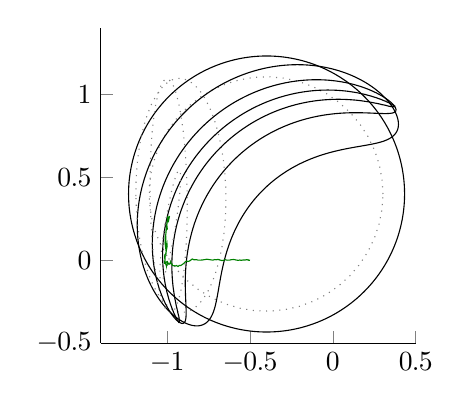
\begin{tikzpicture}

\begin{axis}[%
width=4cm,
height=4cm,
colormap={mymap}{[1pt] rgb(0pt)=(0,0,0); rgb(1pt)=(0,0,0)},
unbounded coords=jump,
scale only axis,
xmin=-1.4,
xmax=0.5,
ymin=-0.5,
ymax=1.4,
axis x line*=bottom,
axis y line*=left
]

\addplot[area legend,solid,draw=black,forget plot]
table[row sep=crcr]{
x y\\
-1.23 0.46490355595815 \\
-1.22960150659877 0.47 \\
-1.22869862032926 0.48 \\
-1.22767371065223 0.49 \\
-1.22652615959779 0.5 \\
-1.22525527442296 0.51 \\
-1.22386028691466 0.52 \\
-1.22234035261571 0.53 \\
-1.22069454997284 0.54 \\
-1.22 0.543925012252854 \\
-1.21892640279752 0.55 \\
-1.21703375996655 0.56 \\
-1.21501255351594 0.57 \\
-1.21286154858517 0.58 \\
-1.21057942808711 0.59 \\
-1.21 0.592406769213231 \\
-1.20817185045267 0.6 \\
-1.20563301512456 0.61 \\
-1.20295912720575 0.62 \\
-1.2001485327529 0.63 \\
-1.2 0.630505916752702 \\
-1.19720927177399 0.64 \\
-1.19413073501926 0.65 \\
-1.19091048235894 0.66 \\
-1.19 0.662717034143122 \\
-1.18755419286408 0.67 \\
-1.1840553713141 0.68 \\
-1.18040895669849 0.69 \\
-1.18 0.691082930921102 \\
-1.1766220430266 0.7 \\
-1.17268437715587 0.71 \\
-1.17 0.716574164360218 \\
-1.16859570678079 0.72 \\
-1.16435686868754 0.73 \\
-1.16 0.739906655398264 \\
-1.15995875610125 0.74 \\
-1.15540766506219 0.75 \\
-1.15069176174176 0.76 \\
-1.15 0.76142534514183 \\
-1.14581495754822 0.77 \\
-1.14076851906906 0.78 \\
-1.14 0.781481800290595 \\
-1.13555370431776 0.79 \\
-1.13016256518617 0.8 \\
-1.13 0.800294055571771 \\
-1.12459541368304 0.81 \\
-1.12 0.818003330802316 \\
-1.11884457213804 0.82 \\
-1.11290789864718 0.83 \\
-1.11 0.834766310779763 \\
-1.1067794262609 0.84 \\
-1.10045499989146 0.85 \\
-1.1 0.85070324293253 \\
-1.09392825155636 0.86 \\
-1.09 0.86585779537492 \\
-1.08719432959242 0.87 \\
-1.0802478170049 0.88 \\
-1.08 0.880349311626938 \\
-1.07307898957916 0.89 \\
-1.07 0.894191086141864 \\
-1.06568343026022 0.9 \\
-1.06 0.907472179329761 \\
-1.0580539964072 0.91 \\
-1.05018227493588 0.92 \\
-1.05 0.920227114822055 \\
-1.0420548844932 0.93 \\
-1.04 0.932474665837886 \\
-1.0336661072561 0.94 \\
-1.03 0.944267684379233 \\
-1.02500542583447 0.95 \\
-1.02 0.955632804221174 \\
-1.01606124067785 0.96 \\
-1.01 0.96659434215035 \\
-1.00682078403302 0.97 \\
-1 0.977174502586599 \\
-0.997270024404195 0.98 \\
-0.99 0.987393560386835 \\
-0.987393560386835 0.99 \\
-0.98 0.997270024404194 \\
-0.977174502586599 1 \\
-0.97 1.00682078403302 \\
-0.96659434215035 1.01 \\
-0.96 1.01606124067785 \\
-0.955632804221174 1.02 \\
-0.95 1.02500542583447 \\
-0.944267684379233 1.03 \\
-0.94 1.0336661072561 \\
-0.932474665837887 1.04 \\
-0.93 1.0420548844932 \\
-0.920227114822055 1.05 \\
-0.92 1.05018227493588 \\
-0.91 1.0580539964072 \\
-0.90747217932976 1.06 \\
-0.9 1.06568343026022 \\
-0.894191086141864 1.07 \\
-0.89 1.07307898957916 \\
-0.880349311626938 1.08 \\
-0.88 1.0802478170049 \\
-0.87 1.08719432959242 \\
-0.86585779537492 1.09 \\
-0.86 1.09392825155636 \\
-0.85070324293253 1.1 \\
-0.85 1.10045499989146 \\
-0.84 1.1067794262609 \\
-0.834766310779763 1.11 \\
-0.83 1.11290789864718 \\
-0.82 1.11884457213804 \\
-0.818003330802316 1.12 \\
-0.81 1.12459541368304 \\
-0.800294055571771 1.13 \\
-0.8 1.13016256518617 \\
-0.79 1.13555370431776 \\
-0.781481800290595 1.14 \\
-0.78 1.14076851906906 \\
-0.77 1.14581495754822 \\
-0.76142534514183 1.15 \\
-0.76 1.15069176174176 \\
-0.75 1.15540766506219 \\
-0.74 1.15995875610125 \\
-0.739906655398264 1.16 \\
-0.73 1.16435686868754 \\
-0.72 1.16859570678079 \\
-0.716574164360217 1.17 \\
-0.71 1.17268437715587 \\
-0.7 1.1766220430266 \\
-0.691082930921101 1.18 \\
-0.69 1.18040895669849 \\
-0.68 1.1840553713141 \\
-0.67 1.18755419286408 \\
-0.662717034143123 1.19 \\
-0.66 1.19091048235894 \\
-0.65 1.19413073501926 \\
-0.64 1.19720927177399 \\
-0.630505916752703 1.2 \\
-0.63 1.2001485327529 \\
-0.62 1.20295912720575 \\
-0.61 1.20563301512456 \\
-0.6 1.20817185045267 \\
-0.592406769213231 1.21 \\
-0.59 1.21057942808711 \\
-0.58 1.21286154858517 \\
-0.57 1.21501255351594 \\
-0.56 1.21703375996655 \\
-0.55 1.21892640279752 \\
-0.543925012252854 1.22 \\
-0.54 1.22069454997284 \\
-0.53 1.22234035261571 \\
-0.52 1.22386028691466 \\
-0.51 1.22525527442296 \\
-0.5 1.22652615959779 \\
-0.49 1.22767371065223 \\
-0.48 1.22869862032926 \\
-0.47 1.22960150659877 \\
-0.46490355595815 1.23 \\
-0.46 1.23038466003635 \\
-0.45 1.23104806991097 \\
-0.44 1.23159031728077 \\
-0.43 1.23201172796599 \\
-0.42 1.23231255504488 \\
-0.41 1.23249297910695 \\
-0.4 1.2325531084337 \\
-0.39 1.23249297910695 \\
-0.38 1.23231255504488 \\
-0.37 1.23201172796599 \\
-0.36 1.23159031728077 \\
-0.35 1.23104806991097 \\
-0.34 1.23038466003635 \\
-0.335096444041851 1.23 \\
-0.33 1.22960150659877 \\
-0.32 1.22869862032926 \\
-0.31 1.22767371065223 \\
-0.3 1.22652615959779 \\
-0.29 1.22525527442296 \\
-0.28 1.22386028691466 \\
-0.27 1.22234035261571 \\
-0.26 1.22069454997284 \\
-0.256074987747147 1.22 \\
-0.25 1.21892640279752 \\
-0.24 1.21703375996655 \\
-0.23 1.21501255351594 \\
-0.22 1.21286154858517 \\
-0.21 1.21057942808711 \\
-0.207593230786769 1.21 \\
-0.2 1.20817185045267 \\
-0.19 1.20563301512456 \\
-0.18 1.20295912720575 \\
-0.17 1.2001485327529 \\
-0.169494083247298 1.2 \\
-0.16 1.19720927177399 \\
-0.15 1.19413073501926 \\
-0.14 1.19091048235894 \\
-0.137282965856877 1.19 \\
-0.13 1.18755419286408 \\
-0.12 1.1840553713141 \\
-0.11 1.18040895669849 \\
-0.108917069078899 1.18 \\
-0.0999999999999999 1.1766220430266 \\
-0.0899999999999999 1.17268437715587 \\
-0.0834258356397825 1.17 \\
-0.0800000000000001 1.16859570678079 \\
-0.0700000000000001 1.16435686868754 \\
-0.0600933446017362 1.16 \\
-0.0600000000000001 1.15995875610125 \\
-0.05 1.15540766506219 \\
-0.04 1.15069176174176 \\
-0.0385746548581699 1.15 \\
-0.03 1.14581495754822 \\
-0.02 1.14076851906906 \\
-0.0185181997094054 1.14 \\
-0.01 1.13555370431776 \\
0 1.13016256518617 \\
0.000294055571771424 1.13 \\
0.01 1.12459541368304 \\
0.0180033308023158 1.12 \\
0.02 1.11884457213804 \\
0.03 1.11290789864718 \\
0.0347663107797624 1.11 \\
0.04 1.1067794262609 \\
0.05 1.10045499989146 \\
0.0507032429325301 1.1 \\
0.0600000000000001 1.09392825155636 \\
0.0658577953749194 1.09 \\
0.0700000000000001 1.08719432959242 \\
0.0800000000000001 1.0802478170049 \\
0.0803493116269377 1.08 \\
0.0899999999999999 1.07307898957916 \\
0.0941910861418636 1.07 \\
0.0999999999999999 1.06568343026022 \\
0.10747217932976 1.06 \\
0.11 1.0580539964072 \\
0.12 1.05018227493588 \\
0.120227114822055 1.05 \\
0.13 1.0420548844932 \\
0.132474665837886 1.04 \\
0.14 1.0336661072561 \\
0.144267684379233 1.03 \\
0.15 1.02500542583447 \\
0.155632804221174 1.02 \\
0.16 1.01606124067785 \\
0.16659434215035 1.01 \\
0.17 1.00682078403302 \\
0.1771745025866 1 \\
0.18 0.997270024404194 \\
0.187393560386835 0.99 \\
0.19 0.987393560386835 \\
0.197270024404195 0.98 \\
0.2 0.977174502586599 \\
0.206820784033018 0.97 \\
0.21 0.96659434215035 \\
0.216061240677853 0.96 \\
0.22 0.955632804221174 \\
0.225005425834474 0.95 \\
0.23 0.944267684379233 \\
0.233666107256098 0.94 \\
0.24 0.932474665837886 \\
0.242054884493204 0.93 \\
0.25 0.920227114822055 \\
0.250182274935881 0.92 \\
0.258053996407202 0.91 \\
0.26 0.907472179329761 \\
0.265683430260224 0.9 \\
0.27 0.894191086141863 \\
0.273078989579159 0.89 \\
0.28 0.880349311626938 \\
0.280247817004903 0.88 \\
0.287194329592418 0.87 \\
0.29 0.865857795374919 \\
0.293928251556358 0.86 \\
0.3 0.85070324293253 \\
0.300454999891464 0.85 \\
0.306779426260899 0.84 \\
0.31 0.834766310779762 \\
0.312907898647181 0.83 \\
0.318844572138043 0.82 \\
0.32 0.818003330802316 \\
0.324595413683044 0.81 \\
0.33 0.800294055571771 \\
0.330162565186173 0.8 \\
0.335553704317761 0.79 \\
0.34 0.781481800290595 \\
0.340768519069056 0.78 \\
0.345814957548218 0.77 \\
0.35 0.76142534514183 \\
0.350691761741762 0.76 \\
0.355407665062195 0.75 \\
0.359958756101252 0.74 \\
0.36 0.739906655398264 \\
0.364356868687543 0.73 \\
0.368595706780788 0.72 \\
0.37 0.716574164360218 \\
0.372684377155872 0.71 \\
0.376622043026596 0.7 \\
0.38 0.691082930921102 \\
0.380408956698492 0.69 \\
0.384055371314095 0.68 \\
0.387554192864077 0.67 \\
0.39 0.662717034143122 \\
0.390910482358941 0.66 \\
0.394130735019259 0.65 \\
0.397209271773994 0.64 \\
0.4 0.630505916752702 \\
0.400148532752897 0.63 \\
0.402959127205753 0.62 \\
0.405633015124562 0.61 \\
0.408171850452672 0.6 \\
0.41 0.592406769213231 \\
0.410579428087114 0.59 \\
0.41286154858517 0.58 \\
0.415012553515935 0.57 \\
0.417033759966547 0.56 \\
0.418926402797516 0.55 \\
0.42 0.543925012252854 \\
0.420694549972838 0.54 \\
0.422340352615714 0.53 \\
0.423860286914664 0.52 \\
0.425255274422965 0.51 \\
0.426526159597789 0.5 \\
0.427673710652226 0.49 \\
0.428698620329256 0.48 \\
0.429601506598767 0.47 \\
0.43 0.46490355595815 \\
0.430384660036347 0.46 \\
0.431048069910975 0.45 \\
0.431590317280767 0.44 \\
0.432011727965991 0.43 \\
0.432312555044877 0.42 \\
0.432492979106945 0.41 \\
0.432553108433699 0.4 \\
0.432492979106945 0.39 \\
0.432312555044877 0.38 \\
0.432011727965991 0.37 \\
0.431590317280767 0.36 \\
0.431048069910975 0.35 \\
0.430384660036347 0.34 \\
0.43 0.335096444041851 \\
0.429601506598767 0.33 \\
0.428698620329256 0.32 \\
0.427673710652226 0.31 \\
0.426526159597789 0.3 \\
0.425255274422965 0.29 \\
0.423860286914664 0.28 \\
0.422340352615714 0.27 \\
0.420694549972838 0.26 \\
0.42 0.256074987747147 \\
0.418926402797516 0.25 \\
0.417033759966547 0.24 \\
0.415012553515935 0.23 \\
0.41286154858517 0.22 \\
0.410579428087114 0.21 \\
0.41 0.207593230786769 \\
0.408171850452672 0.2 \\
0.405633015124562 0.19 \\
0.402959127205753 0.18 \\
0.400148532752897 0.17 \\
0.4 0.169494083247298 \\
0.397209271773994 0.16 \\
0.394130735019258 0.15 \\
0.390910482358941 0.14 \\
0.39 0.137282965856877 \\
0.387554192864077 0.13 \\
0.384055371314095 0.12 \\
0.380408956698492 0.11 \\
0.38 0.108917069078899 \\
0.376622043026596 0.0999999999999999 \\
0.372684377155872 0.0899999999999999 \\
0.37 0.0834258356397825 \\
0.368595706780788 0.0800000000000001 \\
0.364356868687543 0.0700000000000001 \\
0.36 0.0600933446017357 \\
0.359958756101252 0.0600000000000001 \\
0.355407665062195 0.05 \\
0.350691761741762 0.04 \\
0.35 0.0385746548581699 \\
0.345814957548218 0.03 \\
0.340768519069056 0.02 \\
0.34 0.0185181997094054 \\
0.335553704317761 0.01 \\
0.330162565186173 0 \\
0.33 -0.000294055571771139 \\
0.324595413683044 -0.01 \\
0.32 -0.0180033308023158 \\
0.318844572138043 -0.02 \\
0.312907898647181 -0.03 \\
0.31 -0.0347663107797621 \\
0.306779426260899 -0.04 \\
0.300454999891464 -0.05 \\
0.3 -0.0507032429325301 \\
0.293928251556357 -0.0600000000000001 \\
0.29 -0.0658577953749191 \\
0.287194329592418 -0.0700000000000001 \\
0.280247817004903 -0.0800000000000001 \\
0.28 -0.0803493116269377 \\
0.273078989579159 -0.0899999999999999 \\
0.27 -0.0941910861418633 \\
0.265683430260224 -0.0999999999999999 \\
0.26 -0.10747217932976 \\
0.258053996407202 -0.11 \\
0.250182274935881 -0.12 \\
0.25 -0.120227114822055 \\
0.242054884493204 -0.13 \\
0.24 -0.132474665837886 \\
0.233666107256098 -0.14 \\
0.23 -0.144267684379233 \\
0.225005425834474 -0.15 \\
0.22 -0.155632804221174 \\
0.216061240677853 -0.16 \\
0.21 -0.16659434215035 \\
0.206820784033018 -0.17 \\
0.2 -0.1771745025866 \\
0.197270024404195 -0.18 \\
0.19 -0.187393560386835 \\
0.187393560386835 -0.19 \\
0.18 -0.197270024404195 \\
0.1771745025866 -0.2 \\
0.17 -0.206820784033018 \\
0.16659434215035 -0.21 \\
0.16 -0.216061240677853 \\
0.155632804221174 -0.22 \\
0.15 -0.225005425834474 \\
0.144267684379233 -0.23 \\
0.14 -0.233666107256098 \\
0.132474665837886 -0.24 \\
0.13 -0.242054884493204 \\
0.120227114822055 -0.25 \\
0.12 -0.250182274935881 \\
0.11 -0.258053996407202 \\
0.10747217932976 -0.26 \\
0.0999999999999999 -0.265683430260224 \\
0.0941910861418633 -0.27 \\
0.0899999999999999 -0.273078989579159 \\
0.0803493116269377 -0.28 \\
0.0800000000000001 -0.280247817004903 \\
0.0700000000000001 -0.287194329592418 \\
0.0658577953749191 -0.29 \\
0.0600000000000001 -0.293928251556357 \\
0.0507032429325301 -0.3 \\
0.05 -0.300454999891464 \\
0.04 -0.306779426260899 \\
0.0347663107797621 -0.31 \\
0.03 -0.312907898647181 \\
0.02 -0.318844572138043 \\
0.0180033308023158 -0.32 \\
0.01 -0.324595413683044 \\
0.000294055571771139 -0.33 \\
0 -0.330162565186173 \\
-0.01 -0.335553704317761 \\
-0.0185181997094054 -0.34 \\
-0.02 -0.340768519069056 \\
-0.03 -0.345814957548218 \\
-0.0385746548581699 -0.35 \\
-0.04 -0.350691761741762 \\
-0.05 -0.355407665062195 \\
-0.0600000000000001 -0.359958756101252 \\
-0.0600933446017357 -0.36 \\
-0.0700000000000001 -0.364356868687543 \\
-0.0800000000000001 -0.368595706780788 \\
-0.0834258356397825 -0.37 \\
-0.0899999999999999 -0.372684377155872 \\
-0.0999999999999999 -0.376622043026596 \\
-0.108917069078899 -0.38 \\
-0.11 -0.380408956698492 \\
-0.12 -0.384055371314095 \\
-0.13 -0.387554192864077 \\
-0.137282965856877 -0.39 \\
-0.14 -0.390910482358941 \\
-0.15 -0.394130735019258 \\
-0.16 -0.397209271773994 \\
-0.169494083247298 -0.4 \\
-0.17 -0.400148532752897 \\
-0.18 -0.402959127205753 \\
-0.19 -0.405633015124562 \\
-0.2 -0.408171850452672 \\
-0.207593230786769 -0.41 \\
-0.21 -0.410579428087114 \\
-0.22 -0.41286154858517 \\
-0.23 -0.415012553515935 \\
-0.24 -0.417033759966547 \\
-0.25 -0.418926402797516 \\
-0.256074987747147 -0.42 \\
-0.26 -0.420694549972838 \\
-0.27 -0.422340352615714 \\
-0.28 -0.423860286914664 \\
-0.29 -0.425255274422965 \\
-0.3 -0.426526159597789 \\
-0.31 -0.427673710652226 \\
-0.32 -0.428698620329256 \\
-0.33 -0.429601506598767 \\
-0.335096444041851 -0.43 \\
-0.34 -0.430384660036347 \\
-0.35 -0.431048069910975 \\
-0.36 -0.431590317280767 \\
-0.37 -0.432011727965991 \\
-0.38 -0.432312555044877 \\
-0.39 -0.432492979106945 \\
-0.4 -0.432553108433699 \\
-0.41 -0.432492979106945 \\
-0.42 -0.432312555044877 \\
-0.43 -0.432011727965991 \\
-0.44 -0.431590317280767 \\
-0.45 -0.431048069910975 \\
-0.46 -0.430384660036347 \\
-0.46490355595815 -0.43 \\
-0.47 -0.429601506598767 \\
-0.48 -0.428698620329256 \\
-0.49 -0.427673710652226 \\
-0.5 -0.426526159597789 \\
-0.51 -0.425255274422965 \\
-0.52 -0.423860286914664 \\
-0.53 -0.422340352615714 \\
-0.54 -0.420694549972838 \\
-0.543925012252854 -0.42 \\
-0.55 -0.418926402797516 \\
-0.56 -0.417033759966547 \\
-0.57 -0.415012553515935 \\
-0.58 -0.41286154858517 \\
-0.59 -0.410579428087114 \\
-0.592406769213231 -0.41 \\
-0.6 -0.408171850452672 \\
-0.61 -0.405633015124562 \\
-0.62 -0.402959127205753 \\
-0.63 -0.400148532752897 \\
-0.630505916752703 -0.4 \\
-0.64 -0.397209271773994 \\
-0.65 -0.394130735019259 \\
-0.66 -0.390910482358941 \\
-0.662717034143123 -0.39 \\
-0.67 -0.387554192864077 \\
-0.68 -0.384055371314095 \\
-0.69 -0.380408956698492 \\
-0.691082930921101 -0.38 \\
-0.7 -0.376622043026596 \\
-0.71 -0.372684377155872 \\
-0.716574164360217 -0.37 \\
-0.72 -0.368595706780788 \\
-0.73 -0.364356868687543 \\
-0.739906655398264 -0.36 \\
-0.74 -0.359958756101252 \\
-0.75 -0.355407665062195 \\
-0.76 -0.350691761741762 \\
-0.76142534514183 -0.35 \\
-0.77 -0.345814957548218 \\
-0.78 -0.340768519069056 \\
-0.781481800290595 -0.34 \\
-0.79 -0.335553704317761 \\
-0.8 -0.330162565186173 \\
-0.800294055571771 -0.33 \\
-0.81 -0.324595413683044 \\
-0.818003330802316 -0.32 \\
-0.82 -0.318844572138043 \\
-0.83 -0.312907898647181 \\
-0.834766310779762 -0.31 \\
-0.84 -0.306779426260899 \\
-0.85 -0.300454999891464 \\
-0.85070324293253 -0.3 \\
-0.86 -0.293928251556358 \\
-0.865857795374919 -0.29 \\
-0.87 -0.287194329592418 \\
-0.88 -0.280247817004903 \\
-0.880349311626938 -0.28 \\
-0.89 -0.273078989579159 \\
-0.894191086141863 -0.27 \\
-0.9 -0.265683430260224 \\
-0.90747217932976 -0.26 \\
-0.91 -0.258053996407202 \\
-0.92 -0.250182274935881 \\
-0.920227114822055 -0.25 \\
-0.93 -0.242054884493204 \\
-0.932474665837887 -0.24 \\
-0.94 -0.233666107256098 \\
-0.944267684379233 -0.23 \\
-0.95 -0.225005425834474 \\
-0.955632804221174 -0.22 \\
-0.96 -0.216061240677853 \\
-0.96659434215035 -0.21 \\
-0.97 -0.206820784033018 \\
-0.977174502586599 -0.2 \\
-0.98 -0.197270024404195 \\
-0.987393560386835 -0.19 \\
-0.99 -0.187393560386835 \\
-0.997270024404195 -0.18 \\
-1 -0.1771745025866 \\
-1.00682078403302 -0.17 \\
-1.01 -0.16659434215035 \\
-1.01606124067785 -0.16 \\
-1.02 -0.155632804221174 \\
-1.02500542583447 -0.15 \\
-1.03 -0.144267684379233 \\
-1.0336661072561 -0.14 \\
-1.04 -0.132474665837886 \\
-1.0420548844932 -0.13 \\
-1.05 -0.120227114822055 \\
-1.05018227493588 -0.12 \\
-1.0580539964072 -0.11 \\
-1.06 -0.10747217932976 \\
-1.06568343026022 -0.0999999999999999 \\
-1.07 -0.0941910861418636 \\
-1.07307898957916 -0.0899999999999999 \\
-1.08 -0.0803493116269377 \\
-1.0802478170049 -0.0800000000000001 \\
-1.08719432959242 -0.0700000000000001 \\
-1.09 -0.0658577953749194 \\
-1.09392825155636 -0.0600000000000001 \\
-1.1 -0.0507032429325301 \\
-1.10045499989146 -0.05 \\
-1.1067794262609 -0.04 \\
-1.11 -0.0347663107797624 \\
-1.11290789864718 -0.03 \\
-1.11884457213804 -0.02 \\
-1.12 -0.0180033308023158 \\
-1.12459541368304 -0.01 \\
-1.13 -0.000294055571771424 \\
-1.13016256518617 0 \\
-1.13555370431776 0.01 \\
-1.14 0.0185181997094054 \\
-1.14076851906906 0.02 \\
-1.14581495754822 0.03 \\
-1.15 0.0385746548581699 \\
-1.15069176174176 0.04 \\
-1.15540766506219 0.05 \\
-1.15995875610125 0.0600000000000001 \\
-1.16 0.0600933446017362 \\
-1.16435686868754 0.0700000000000001 \\
-1.16859570678079 0.0800000000000001 \\
-1.17 0.0834258356397825 \\
-1.17268437715587 0.0899999999999999 \\
-1.1766220430266 0.0999999999999999 \\
-1.18 0.108917069078899 \\
-1.18040895669849 0.11 \\
-1.1840553713141 0.12 \\
-1.18755419286408 0.13 \\
-1.19 0.137282965856877 \\
-1.19091048235894 0.14 \\
-1.19413073501926 0.15 \\
-1.19720927177399 0.16 \\
-1.2 0.169494083247298 \\
-1.2001485327529 0.17 \\
-1.20295912720575 0.18 \\
-1.20563301512456 0.19 \\
-1.20817185045267 0.2 \\
-1.21 0.207593230786769 \\
-1.21057942808711 0.21 \\
-1.21286154858517 0.22 \\
-1.21501255351594 0.23 \\
-1.21703375996655 0.24 \\
-1.21892640279752 0.25 \\
-1.22 0.256074987747147 \\
-1.22069454997284 0.26 \\
-1.22234035261571 0.27 \\
-1.22386028691466 0.28 \\
-1.22525527442296 0.29 \\
-1.22652615959779 0.3 \\
-1.22767371065223 0.31 \\
-1.22869862032926 0.32 \\
-1.22960150659877 0.33 \\
-1.23 0.335096444041851 \\
-1.23038466003635 0.34 \\
-1.23104806991097 0.35 \\
-1.23159031728077 0.36 \\
-1.23201172796599 0.37 \\
-1.23231255504488 0.38 \\
-1.23249297910694 0.39 \\
-1.2325531084337 0.4 \\
-1.23249297910694 0.41 \\
-1.23231255504488 0.42 \\
-1.23201172796599 0.43 \\
-1.23159031728077 0.44 \\
-1.23104806991097 0.45 \\
-1.23038466003635 0.46 \\
-1.23 0.46490355595815 \\
NaN NaN \\
};

\addplot [
color=gray,
dotted,
forget plot
]
table[row sep=crcr]{
0.302360541231733 0.4\\
0.2965696634757 0.490422808186003\\
0.279292116260257 0.579360876361465\\
0.250811596433019 0.665353843905771\\
0.211595753342162 0.746989708669247\\
0.162288510047058 0.822928012009422\\
0.10369949011944 0.891921849084879\\
0.0367907236467382 0.952838342998275\\
-0.0373391492753579 1.00467724660368\\
-0.117472918182899 1.04658736653706\\
-0.202294788805839 1.07788053978777\\
-0.290411988373579 1.09804293331619\\
-0.380377634905347 1.10674348117799\\
-0.470714494972326 1.10383932061783\\
-0.559939239829713 1.08937813787181\\
-0.646586801633701 1.06359738516082\\
-0.729234429814971 1.02692038173164\\
-0.806525052603702 0.979949362966567\\
-0.877189560110518 0.923455591695151\\
-0.940067643075783 0.858366694079811\\
-0.994126845115566 0.785751428019912\\
-1.03847951562692 0.7068021341766\\
-1.07239738498625 0.622815157772112\\
-1.09532352271638 0.535169562637062\\
-1.1068814822696 0.445304487020476\\
-1.1068814822696 0.354695512979524\\
-1.09532352271638 0.264830437362938\\
-1.07239738498625 0.177184842227889\\
-1.03847951562692 0.0931978658233998\\
-0.994126845115566 0.0142485719800879\\
-0.940067643075784 -0.058366694079811\\
-0.877189560110518 -0.123455591695151\\
-0.806525052603702 -0.179949362966567\\
-0.729234429814971 -0.226920381731638\\
-0.646586801633701 -0.263597385160825\\
-0.559939239829713 -0.28937813787181\\
-0.470714494972325 -0.303839320617828\\
-0.380377634905347 -0.30674348117799\\
-0.29041198837358 -0.298042933316187\\
-0.20229478880584 -0.277880539787771\\
-0.117472918182899 -0.246587366537059\\
-0.0373391492753583 -0.204677246603681\\
0.036790723646738 -0.152838342998275\\
0.103699490119439 -0.0919218490848791\\
0.162288510047058 -0.0229280120094228\\
0.211595753342162 0.0530102913307532\\
0.250811596433019 0.134646156094229\\
0.279292116260257 0.220639123638535\\
0.2965696634757 0.309577191813997\\
0.302360541231733 0.4\\
};

\addplot[area legend,solid,draw=black,forget plot]
table[row sep=crcr]{
x y\\
-1.17 0.34824483234669 \\
-1.16974685063192 0.35 \\
-1.16819226362119 0.36 \\
-1.16652579083749 0.37 \\
-1.16474640465062 0.38 \\
-1.16285290186727 0.39 \\
-1.16084389340103 0.4 \\
-1.16 0.403972283004096 \\
-1.15872752024962 0.41 \\
-1.15650161857746 0.42 \\
-1.15415850992452 0.43 \\
-1.15169620345948 0.44 \\
-1.15 0.446570497508841 \\
-1.14911957270876 0.45 \\
-1.14643582378503 0.46 \\
-1.14362995065294 0.47 \\
-1.14069920346947 0.48 \\
-1.14 0.482292669864651 \\
-1.13766087050511 0.49 \\
-1.13450203673762 0.5 \\
-1.13121376409444 0.51 \\
-1.13 0.513558350248353 \\
-1.1278116203584 0.52 \\
-1.12428796612075 0.53 \\
-1.12062893201116 0.54 \\
-1.12 0.541663477723823 \\
-1.11685840800488 0.55 \\
-1.11295502020046 0.56 \\
-1.11 0.56731503463497 \\
-1.1089179667055 0.57 \\
-1.10476285025168 0.58 \\
-1.10046101620946 0.59 \\
-1.1 0.591041770839401 \\
-1.09604227319328 0.6 \\
-1.09147623443274 0.61 \\
-1.09 0.613142166756836 \\
-1.08678076273977 0.62 \\
-1.08194080954232 0.63 \\
-1.08 0.633899158806308 \\
-1.07696335112985 0.64 \\
-1.07183867003779 0.65 \\
-1.07 0.653493256137173 \\
-1.06657249843507 0.66 \\
-1.06115098587887 0.67 \\
-1.06 0.672071557680547 \\
-1.05558789116181 0.68 \\
-1.05 0.689751052742826 \\
-1.04985699636204 0.69 \\
-1.04398616547374 0.7 \\
-1.04 0.706603959589081 \\
-1.03794361838801 0.71 \\
-1.03174054970386 0.72 \\
-1.03 0.722741706044418 \\
-1.02537385112673 0.73 \\
-1.02 0.738216777058695 \\
-1.01882821800339 0.74 \\
-1.01211523648097 0.75 \\
-1.01 0.753080756290404 \\
-1.00522296955145 0.76 \\
-1 0.767388077842723 \\
-0.998141887321532 0.77 \\
-0.990874145928976 0.78 \\
-0.99 0.781179799014672 \\
-0.983418455088601 0.79 \\
-0.98 0.794483082457343 \\
-0.975760203119438 0.8 \\
-0.97 0.807340585135123 \\
-0.967895220180388 0.81 \\
-0.96 0.819777404251693 \\
-0.959818579796784 0.82 \\
-0.951530102936964 0.83 \\
-0.95 0.831812067722366 \\
-0.943015865809287 0.84 \\
-0.94 0.843472184497663 \\
-0.934268290314526 0.85 \\
-0.93 0.854777416654995 \\
-0.925279730157293 0.86 \\
-0.92 0.865745241610559 \\
-0.916041674018024 0.87 \\
-0.91 0.876391723329543 \\
-0.906544708951422 0.88 \\
-0.9 0.886731619659182 \\
-0.896778476336056 0.89 \\
-0.89 0.896778476336056 \\
-0.886731619659182 0.9 \\
-0.88 0.906544708951422 \\
-0.876391723329543 0.91 \\
-0.87 0.916041674018024 \\
-0.865745241610559 0.92 \\
-0.86 0.925279730157293 \\
-0.854777416654995 0.93 \\
-0.85 0.934268290314526 \\
-0.843472184497663 0.94 \\
-0.84 0.943015865809288 \\
-0.831812067722366 0.95 \\
-0.83 0.951530102936965 \\
-0.82 0.959818579796784 \\
-0.819777404251693 0.96 \\
-0.81 0.967895220180388 \\
-0.807340585135122 0.97 \\
-0.8 0.975760203119437 \\
-0.794483082457343 0.98 \\
-0.79 0.983418455088602 \\
-0.781179799014672 0.99 \\
-0.78 0.990874145928976 \\
-0.77 0.998141887321532 \\
-0.767388077842723 1 \\
-0.76 1.00522296955145 \\
-0.753080756290404 1.01 \\
-0.75 1.01211523648097 \\
-0.74 1.01882821800339 \\
-0.738216777058696 1.02 \\
-0.73 1.02537385112673 \\
-0.722741706044418 1.03 \\
-0.72 1.03174054970386 \\
-0.71 1.03794361838801 \\
-0.706603959589081 1.04 \\
-0.7 1.04398616547375 \\
-0.69 1.04985699636204 \\
-0.689751052742826 1.05 \\
-0.68 1.05558789116181 \\
-0.672071557680547 1.06 \\
-0.67 1.06115098587887 \\
-0.66 1.06657249843507 \\
-0.653493256137172 1.07 \\
-0.65 1.07183867003779 \\
-0.64 1.07696335112985 \\
-0.633899158806308 1.08 \\
-0.63 1.08194080954232 \\
-0.62 1.08678076273977 \\
-0.613142166756836 1.09 \\
-0.61 1.09147623443274 \\
-0.6 1.09604227319328 \\
-0.591041770839401 1.1 \\
-0.59 1.10046101620946 \\
-0.58 1.10476285025168 \\
-0.57 1.1089179667055 \\
-0.56731503463497 1.11 \\
-0.56 1.11295502020045 \\
-0.55 1.11685840800488 \\
-0.541663477723823 1.12 \\
-0.54 1.12062893201116 \\
-0.53 1.12428796612075 \\
-0.52 1.1278116203584 \\
-0.513558350248353 1.13 \\
-0.51 1.13121376409444 \\
-0.5 1.13450203673762 \\
-0.49 1.13766087050511 \\
-0.482292669864651 1.14 \\
-0.48 1.14069920346947 \\
-0.47 1.14362995065294 \\
-0.46 1.14643582378503 \\
-0.45 1.14911957270876 \\
-0.446570497508841 1.15 \\
-0.44 1.15169620345948 \\
-0.43 1.15415850992452 \\
-0.42 1.15650161857746 \\
-0.41 1.15872752024962 \\
-0.403972283004096 1.16 \\
-0.4 1.16084389340103 \\
-0.39 1.16285290186727 \\
-0.38 1.16474640465062 \\
-0.37 1.16652579083749 \\
-0.36 1.16819226362119 \\
-0.35 1.16974685063192 \\
-0.34824483234669 1.17 \\
-0.34 1.17119736332875 \\
-0.33 1.17253708306572 \\
-0.32 1.17376516554583 \\
-0.31 1.17488223536639 \\
-0.3 1.17588878364361 \\
-0.29 1.17678517647896 \\
-0.28 1.17757166314514 \\
-0.27 1.17824838400104 \\
-0.26 1.17881537814023 \\
-0.25 1.17927259077445 \\
-0.24 1.17961988034923 \\
-0.23 1.1798570253855 \\
-0.22 1.17998373103776 \\
-0.21 1.17999963535578 \\
-0.2 1.17990431523439 \\
-0.19 1.17969729203277 \\
-0.18 1.17937803684251 \\
-0.17 1.17894597538143 \\
-0.16 1.17840049248854 \\
-0.15 1.17774093619399 \\
-0.14 1.1769666213368 \\
-0.13 1.17607683270263 \\
-0.12 1.17507082765349 \\
-0.11 1.17394783822133 \\
-0.0999999999999999 1.17270707263833 \\
-0.0899999999999999 1.17134771627709 \\
-0.0808808221553111 1.17 \\
-0.0800000000000001 1.169868446055 \\
-0.0700000000000001 1.16826318492631 \\
-0.0600000000000001 1.1665358522753 \\
-0.05 1.16468558953898 \\
-0.04 1.16271152558355 \\
-0.03 1.16061277372685 \\
-0.0272297162274458 1.16 \\
-0.02 1.15837707043464 \\
-0.01 1.15600950424899 \\
0 1.15351353518583 \\
0.01 1.15088831903331 \\
0.0132417961451759 1.15 \\
0.02 1.1481144843506 \\
0.03 1.1451998014171 \\
0.04 1.14215236860539 \\
0.0467845809778874 1.14 \\
0.05 1.13895839590464 \\
0.0600000000000001 1.13560172760492 \\
0.0700000000000001 1.13210924568362 \\
0.0758326192762357 1.13 \\
0.0800000000000001 1.12845705211644 \\
0.0899999999999999 1.12463447377779 \\
0.0999999999999999 1.12067372352401 \\
0.101654875861228 1.12 \\
0.11 1.11651329321956 \\
0.12 1.11220142977958 \\
0.124965625555616 1.11 \\
0.13 1.10770379085866 \\
0.14 1.10302068977659 \\
0.146281627658991 1.1 \\
0.15 1.09815606221167 \\
0.16 1.09308122969512 \\
0.165927999060679 1.09 \\
0.17 1.08781244454026 \\
0.18 1.08232554760214 \\
0.18415237085094 1.08 \\
0.19 1.07660791404929 \\
0.2 1.07068940384791 \\
0.201145721652617 1.07 \\
0.21 1.06447069599288 \\
0.217032177449418 1.06 \\
0.22 1.05803665457619 \\
0.23 1.05132313374821 \\
0.231943882101265 1.05 \\
0.24 1.04428372571177 \\
0.245958520328016 1.04 \\
0.25 1.03696310983243 \\
0.259164215758356 1.03 \\
0.26 1.02933444169534 \\
0.27 1.02130039326315 \\
0.27160451321306 1.02 \\
0.28 1.01285817275248 \\
0.283336244087455 1.01 \\
0.29 1.0039916294524 \\
0.29440365869371 1 \\
0.3 0.994646303613179 \\
0.30483949801983 0.99 \\
0.31 0.984756110397065 \\
0.314671396184423 0.98 \\
0.32 0.974240900702571 \\
0.323922474439262 0.97 \\
0.33 0.963003381220004 \\
0.332611869145027 0.96 \\
0.34 0.950925197880764 \\
0.340755206485876 0.95 \\
0.348353919103909 0.94 \\
0.35 0.937660090845779 \\
0.355419004395882 0.93 \\
0.36 0.922984220900905 \\
0.361962087595305 0.92 \\
0.36797165252887 0.91 \\
0.37 0.906270424491979 \\
0.373443745141697 0.9 \\
0.378378429548447 0.89 \\
0.38 0.8862599122459 \\
0.382748545988888 0.88 \\
0.386543456781287 0.87 \\
0.389749012796172 0.86 \\
0.39 0.859001026024989 \\
0.392300698766757 0.85 \\
0.394180890645867 0.84 \\
0.395336251754202 0.83 \\
0.395697015250948 0.82 \\
0.395176614410703 0.81 \\
0.39366754926419 0.8 \\
0.391035889986567 0.79 \\
0.39 0.787258661419913 \\
0.38705697916176 0.78 \\
0.381513307702241 0.77 \\
0.38 0.76784594377993 \\
0.374007445086244 0.76 \\
0.37 0.7557514351253 \\
0.364054295499889 0.75 \\
0.36 0.746700822030463 \\
0.350894547332186 0.74 \\
0.35 0.739430738915723 \\
0.34 0.733546956944958 \\
0.333298499271874 0.73 \\
0.33 0.728449374871357 \\
0.32 0.724105387704512 \\
0.31 0.720189628818945 \\
0.30948537538196 0.72 \\
0.3 0.716820146879085 \\
0.29 0.713742733243921 \\
0.28 0.710905686344939 \\
0.276631981808553 0.71 \\
0.27 0.708348249786546 \\
0.26 0.705990225868927 \\
0.25 0.703765986162755 \\
0.24 0.701653387666864 \\
0.231856513506836 0.7 \\
0.23 0.699645189000129 \\
0.22 0.697762633450779 \\
0.21 0.695933040344062 \\
0.2 0.694143056983395 \\
0.19 0.692380555671002 \\
0.18 0.690634479159236 \\
0.176397789260313 0.69 \\
0.17 0.688922459583778 \\
0.16 0.687221648864136 \\
0.15 0.685507533384693 \\
0.14 0.683772550733038 \\
0.13 0.682009658682955 \\
0.12 0.680212272727076 \\
0.118859861177737 0.68 \\
0.11 0.678404402725216 \\
0.0999999999999999 0.676553533757192 \\
0.0899999999999999 0.674650364964621 \\
0.0800000000000001 0.672689883309064 \\
0.0700000000000001 0.670667299751165 \\
0.0668306100783585 0.67 \\
0.0600000000000001 0.668597853651372 \\
0.05 0.66646691237605 \\
0.04 0.664260949803104 \\
0.03 0.661976004677973 \\
0.0216673934388655 0.66 \\
0.02 0.659612293922447 \\
0.01 0.657183320094115 \\
0 0.65466475610035 \\
-0.01 0.652053104374175 \\
-0.017567454667616 0.65 \\
-0.02 0.649349850941758 \\
-0.03 0.646563140809441 \\
-0.04 0.643674188237087 \\
-0.05 0.640679674329226 \\
-0.052180207372021 0.64 \\
-0.0600000000000001 0.637589219183333 \\
-0.0700000000000001 0.63439166581964 \\
-0.0800000000000001 0.631080205491351 \\
-0.0831402257352855 0.63 \\
-0.0899999999999999 0.627659442913738 \\
-0.0999999999999999 0.624123550351529 \\
-0.11 0.620465748641229 \\
-0.111227012060718 0.62 \\
-0.12 0.616688410403288 \\
-0.13 0.612785488763925 \\
-0.136900064685736 0.61 \\
-0.14 0.60875277155352 \\
-0.15 0.604588741202766 \\
-0.16 0.600290571267089 \\
-0.16065351031315 0.6 \\
-0.17 0.595850011960966 \\
-0.18 0.591270707191558 \\
-0.182687213649655 0.59 \\
-0.19 0.586540695511637 \\
-0.2 0.581664556411378 \\
-0.203310270220351 0.58 \\
-0.21 0.576629475148341 \\
-0.22 0.571440830887073 \\
-0.222695730199283 0.57 \\
-0.23 0.566082636343688 \\
-0.24 0.56056576211472 \\
-0.240996536634055 0.56 \\
-0.25 0.554864283969042 \\
-0.25829823208705 0.55 \\
-0.26 0.548996397299665 \\
-0.27 0.542936451594461 \\
-0.274718974924906 0.54 \\
-0.28 0.53669018665601 \\
-0.29 0.530259090650918 \\
-0.290392682652562 0.53 \\
-0.3 0.523608996367508 \\
-0.305292522306472 0.52 \\
-0.31 0.516760031015857 \\
-0.31958736311537 0.51 \\
-0.32 0.509706038368183 \\
-0.33 0.502411592496721 \\
-0.333230504355639 0.5 \\
-0.34 0.494889881614602 \\
-0.346333666426978 0.49 \\
-0.35 0.487135070921797 \\
-0.358933405813462 0.48 \\
-0.36 0.479137028373567 \\
-0.37 0.470872491657892 \\
-0.371034071904004 0.47 \\
-0.38 0.462330832836047 \\
-0.382670783399685 0.46 \\
-0.39 0.45351036479971 \\
-0.393888241389502 0.45 \\
-0.4 0.444397399512695 \\
-0.404707850571412 0.44 \\
-0.41 0.434977128695799 \\
-0.415149914587216 0.43 \\
-0.42 0.425233637932722 \\
-0.425233637932722 0.42 \\
-0.43 0.415149914587216 \\
-0.434977128695799 0.41 \\
-0.44 0.404707850571412 \\
-0.444397399512695 0.4 \\
-0.45 0.393888241389502 \\
-0.45351036479971 0.39 \\
-0.46 0.382670783399685 \\
-0.462330832836047 0.38 \\
-0.47 0.371034071904004 \\
-0.470872491657892 0.37 \\
-0.479137028373567 0.36 \\
-0.48 0.358933405813462 \\
-0.487135070921797 0.35 \\
-0.49 0.346333666426978 \\
-0.494889881614602 0.34 \\
-0.5 0.333230504355639 \\
-0.502411592496721 0.33 \\
-0.509706038368183 0.32 \\
-0.51 0.31958736311537 \\
-0.516760031015857 0.31 \\
-0.52 0.305292522306472 \\
-0.523608996367508 0.3 \\
-0.53 0.290392682652562 \\
-0.530259090650918 0.29 \\
-0.53669018665601 0.28 \\
-0.54 0.274718974924906 \\
-0.542936451594461 0.27 \\
-0.548996397299665 0.26 \\
-0.55 0.25829823208705 \\
-0.554864283969042 0.25 \\
-0.56 0.240996536634055 \\
-0.560565762114719 0.24 \\
-0.566082636343688 0.23 \\
-0.57 0.222695730199283 \\
-0.571440830887073 0.22 \\
-0.576629475148341 0.21 \\
-0.58 0.203310270220351 \\
-0.581664556411378 0.2 \\
-0.586540695511637 0.19 \\
-0.59 0.182687213649655 \\
-0.591270707191558 0.18 \\
-0.595850011960966 0.17 \\
-0.6 0.16065351031315 \\
-0.600290571267089 0.16 \\
-0.604588741202766 0.15 \\
-0.60875277155352 0.14 \\
-0.61 0.136900064685736 \\
-0.612785488763925 0.13 \\
-0.616688410403289 0.12 \\
-0.62 0.111227012060718 \\
-0.620465748641228 0.11 \\
-0.624123550351529 0.0999999999999999 \\
-0.627659442913738 0.0899999999999999 \\
-0.63 0.0831402257352855 \\
-0.631080205491351 0.0800000000000001 \\
-0.63439166581964 0.0700000000000001 \\
-0.637589219183333 0.0600000000000001 \\
-0.64 0.052180207372021 \\
-0.640679674329226 0.05 \\
-0.643674188237087 0.04 \\
-0.64656314080944 0.03 \\
-0.649349850941758 0.02 \\
-0.65 0.017567454667616 \\
-0.652053104374176 0.01 \\
-0.654664756100351 0 \\
-0.657183320094115 -0.01 \\
-0.659612293922446 -0.02 \\
-0.66 -0.0216673934388655 \\
-0.661976004677973 -0.03 \\
-0.664260949803104 -0.04 \\
-0.66646691237605 -0.05 \\
-0.668597853651372 -0.0600000000000001 \\
-0.67 -0.0668306100783585 \\
-0.670667299751165 -0.0700000000000001 \\
-0.672689883309064 -0.0800000000000001 \\
-0.674650364964621 -0.0899999999999999 \\
-0.676553533757192 -0.0999999999999999 \\
-0.678404402725216 -0.11 \\
-0.68 -0.118859861177737 \\
-0.680212272727076 -0.12 \\
-0.682009658682955 -0.13 \\
-0.683772550733038 -0.14 \\
-0.685507533384693 -0.15 \\
-0.687221648864136 -0.16 \\
-0.688922459583777 -0.17 \\
-0.69 -0.176397789260313 \\
-0.690634479159236 -0.18 \\
-0.692380555671002 -0.19 \\
-0.694143056983395 -0.2 \\
-0.695933040344063 -0.21 \\
-0.697762633450779 -0.22 \\
-0.699645189000129 -0.23 \\
-0.7 -0.231856513506836 \\
-0.701653387666865 -0.24 \\
-0.703765986162755 -0.25 \\
-0.705990225868927 -0.26 \\
-0.708348249786546 -0.27 \\
-0.71 -0.276631981808553 \\
-0.71090568634494 -0.28 \\
-0.713742733243921 -0.29 \\
-0.716820146879085 -0.3 \\
-0.72 -0.30948537538196 \\
-0.720189628818945 -0.31 \\
-0.724105387704512 -0.32 \\
-0.728449374871357 -0.33 \\
-0.73 -0.333298499271874 \\
-0.733546956944958 -0.34 \\
-0.739430738915724 -0.35 \\
-0.74 -0.350894547332186 \\
-0.746700822030463 -0.36 \\
-0.75 -0.364054295499889 \\
-0.7557514351253 -0.37 \\
-0.76 -0.374007445086244 \\
-0.767845943779929 -0.38 \\
-0.77 -0.381513307702241 \\
-0.78 -0.38705697916176 \\
-0.787258661419913 -0.39 \\
-0.79 -0.391035889986567 \\
-0.8 -0.39366754926419 \\
-0.81 -0.395176614410703 \\
-0.82 -0.395697015250948 \\
-0.83 -0.395336251754202 \\
-0.84 -0.394180890645867 \\
-0.85 -0.392300698766757 \\
-0.859001026024989 -0.39 \\
-0.86 -0.389749012796172 \\
-0.87 -0.386543456781287 \\
-0.88 -0.382748545988888 \\
-0.8862599122459 -0.38 \\
-0.89 -0.378378429548447 \\
-0.9 -0.373443745141697 \\
-0.906270424491979 -0.37 \\
-0.91 -0.36797165252887 \\
-0.92 -0.361962087595305 \\
-0.922984220900905 -0.36 \\
-0.93 -0.355419004395882 \\
-0.93766009084578 -0.35 \\
-0.94 -0.348353919103909 \\
-0.95 -0.340755206485876 \\
-0.950925197880764 -0.34 \\
-0.96 -0.332611869145027 \\
-0.963003381220003 -0.33 \\
-0.97 -0.323922474439262 \\
-0.974240900702571 -0.32 \\
-0.98 -0.314671396184423 \\
-0.984756110397065 -0.31 \\
-0.99 -0.30483949801983 \\
-0.994646303613179 -0.3 \\
-1 -0.29440365869371 \\
-1.0039916294524 -0.29 \\
-1.01 -0.283336244087455 \\
-1.01285817275248 -0.28 \\
-1.02 -0.27160451321306 \\
-1.02130039326315 -0.27 \\
-1.02933444169534 -0.26 \\
-1.03 -0.259164215758356 \\
-1.03696310983243 -0.25 \\
-1.04 -0.245958520328016 \\
-1.04428372571177 -0.24 \\
-1.05 -0.231943882101265 \\
-1.05132313374821 -0.23 \\
-1.05803665457619 -0.22 \\
-1.06 -0.217032177449418 \\
-1.06447069599288 -0.21 \\
-1.07 -0.201145721652617 \\
-1.07068940384791 -0.2 \\
-1.07660791404929 -0.19 \\
-1.08 -0.18415237085094 \\
-1.08232554760214 -0.18 \\
-1.08781244454026 -0.17 \\
-1.09 -0.165927999060679 \\
-1.09308122969512 -0.16 \\
-1.09815606221167 -0.15 \\
-1.1 -0.146281627658991 \\
-1.10302068977659 -0.14 \\
-1.10770379085866 -0.13 \\
-1.11 -0.124965625555616 \\
-1.11220142977958 -0.12 \\
-1.11651329321956 -0.11 \\
-1.12 -0.101654875861228 \\
-1.12067372352401 -0.0999999999999999 \\
-1.12463447377779 -0.0899999999999999 \\
-1.12845705211644 -0.0800000000000001 \\
-1.13 -0.0758326192762357 \\
-1.13210924568362 -0.0700000000000001 \\
-1.13560172760492 -0.0600000000000001 \\
-1.13895839590464 -0.05 \\
-1.14 -0.0467845809778874 \\
-1.14215236860539 -0.04 \\
-1.1451998014171 -0.03 \\
-1.1481144843506 -0.02 \\
-1.15 -0.0132417961451759 \\
-1.15088831903331 -0.01 \\
-1.15351353518583 0 \\
-1.15600950424899 0.01 \\
-1.15837707043464 0.02 \\
-1.16 0.0272297162274458 \\
-1.16061277372685 0.03 \\
-1.16271152558355 0.04 \\
-1.16468558953898 0.05 \\
-1.1665358522753 0.0600000000000001 \\
-1.16826318492631 0.0700000000000001 \\
-1.169868446055 0.0800000000000001 \\
-1.17 0.0808808221553111 \\
-1.17134771627709 0.0899999999999999 \\
-1.17270707263833 0.0999999999999999 \\
-1.17394783822133 0.11 \\
-1.17507082765349 0.12 \\
-1.17607683270263 0.13 \\
-1.1769666213368 0.14 \\
-1.17774093619399 0.15 \\
-1.17840049248854 0.16 \\
-1.17894597538143 0.17 \\
-1.17937803684251 0.18 \\
-1.17969729203277 0.19 \\
-1.17990431523439 0.2 \\
-1.17999963535578 0.21 \\
-1.17998373103776 0.22 \\
-1.1798570253855 0.23 \\
-1.17961988034923 0.24 \\
-1.17927259077445 0.25 \\
-1.17881537814023 0.26 \\
-1.17824838400104 0.27 \\
-1.17757166314514 0.28 \\
-1.17678517647896 0.29 \\
-1.17588878364361 0.3 \\
-1.17488223536639 0.31 \\
-1.17376516554583 0.32 \\
-1.17253708306572 0.33 \\
-1.17119736332875 0.34 \\
-1.17 0.34824483234669 \\
NaN NaN \\
};

\addplot [
color=gray,
dotted,
forget plot
]
table[row sep=crcr]{
-1.18816259276298 0.387660825716958\\
-1.1872623009542 0.478024200150298\\
-1.18191806302077 0.566969413672885\\
-1.17221763120181 0.653035988337699\\
-1.15832028631961 0.734810713368186\\
-1.14045422239291 0.810950850040126\\
-1.11891279969747 0.880206179414376\\
-1.09404972779839 0.941439530897277\\
-1.06627325764888 0.993645454550367\\
-1.03603947812088 1.03596673055057\\
-1.00384482703837 1.06770844471601\\
-0.970217939682064 1.08834939897762\\
-0.935710968612685 1.09755066943708\\
-0.900890517341195 1.09516117148784\\
-0.86632833671481 1.08122014062015\\
-0.83259193678389 1.05595648817544\\
-0.800235268302609 1.01978504262841\\
-0.769789626872881 0.97329973811492\\
-0.741754929085267 0.917263862049928\\
-0.716591503902378 0.852597521969227\\
-0.694712534070037 0.780362537389144\\
-0.676477271668014 0.701745004759439\\
-0.662185139200809 0.618035821792394\\
-0.652070813088407 0.530609490958062\\
-0.646300370285948 0.440901550191711\\
-0.644968561304716 0.350385001400616\\
-0.648097254411361 0.26054612381346\\
-0.655635076551572 0.172860069316495\\
-0.667458256894199 0.0887666405003501\\
-0.683372659144886 0.00964664914129715\\
-0.703116969258655 -0.0632007566899383\\
-0.726366986209299 -0.128579424603582\\
-0.752740945361268 -0.185415838679984\\
-0.781805787034435 -0.232776746571336\\
-0.813084267332069 -0.269884483479426\\
-0.846062794472421 -0.296129741390121\\
-0.880199861951588 -0.311081573894117\\
-0.914934940065332 -0.314494472315065\\
-0.949697679791329 -0.306312396955246\\
-0.983917277904345 -0.286669697265864\\
-1.01703184954942 -0.255888905832766\\
-1.04849765437563 -0.214475442400303\\
-1.07779802473767 -0.163109314893099\\
-1.10445184936423 -0.102633953704729\\
-1.12802147319183 -0.0340423625939751\\
-1.14811988364885 0.0415391864094429\\
-1.16441706539122 0.122869646360451\\
-1.17664541914529 0.208613573355158\\
-1.18460415568051 0.297363054482828\\
-1.18816259276298 0.387660825716957\\
};

\addplot[area legend,solid,draw=black,forget plot]
table[row sep=crcr]{
x y\\
-1.08 0.231100501158994 \\
-1.07871196895865 0.24 \\
-1.07715886677485 0.25 \\
-1.07549877520187 0.26 \\
-1.073729226905 0.27 \\
-1.07184711715049 0.28 \\
-1.07 0.28924301708876 \\
-1.0698500519161 0.29 \\
-1.06775793738537 0.3 \\
-1.06555568832225 0.31 \\
-1.06323842644563 0.32 \\
-1.06080035677995 0.33 \\
-1.06 0.333127338095644 \\
-1.05826036304034 0.34 \\
-1.05561488001036 0.35 \\
-1.05284770266877 0.36 \\
-1.05 0.369828745506068 \\
-1.04995085831684 0.37 \\
-1.04696825367183 0.38 \\
-1.04386103713728 0.39 \\
-1.04061806973452 0.4 \\
-1.04 0.40183437771208 \\
-1.03727957536703 0.41 \\
-1.03381936150804 0.42 \\
-1.0302140006715 0.43 \\
-1.03 0.430573570296294 \\
-1.02652185472898 0.44 \\
-1.02269099497391 0.45 \\
-1.02 0.456764849853095 \\
-1.01872477090524 0.46 \\
-1.01465772283711 0.47 \\
-1.01043012432748 0.48 \\
-1.01 0.480986835601705 \\
-1.0061091515928 0.49 \\
-1.001633452438 0.5 \\
-1 0.503534272941972 \\
-0.997036250928217 0.51 \\
-0.992300523762823 0.52 \\
-0.99 0.524702421819395 \\
-0.987426657057749 0.53 \\
-0.98241805132332 0.54 \\
-0.98 0.544677085422287 \\
-0.97726492395677 0.55 \\
-0.971968814856949 0.56 \\
-0.97 0.563609163138297 \\
-0.966532331088546 0.57 \\
-0.96093124959039 0.58 \\
-0.96 0.581620338708095 \\
-0.95520622028468 0.59 \\
-0.95 0.598802014012256 \\
-0.949293091822093 0.6 \\
-0.943258836531548 0.61 \\
-0.94 0.615238610570856 \\
-0.937043596862247 0.62 \\
-0.930655644188156 0.63 \\
-0.93 0.631003486606561 \\
-0.924129990682321 0.64 \\
-0.92 0.646145788544833 \\
-0.917408840785191 0.65 \\
-0.910507261450283 0.66 \\
-0.91 0.660719880676243 \\
-0.903454781809262 0.67 \\
-0.9 0.674768258275351 \\
-0.896199953338119 0.68 \\
-0.89 0.688321971589354 \\
-0.888744907651233 0.69 \\
-0.881108320144735 0.7 \\
-0.88 0.701421472456822 \\
-0.873281237105897 0.71 \\
-0.87 0.714093916723676 \\
-0.865238705316014 0.72 \\
-0.86 0.726358323860261 \\
-0.85697830205961 0.73 \\
-0.85 0.738239009950063 \\
-0.848496131171515 0.74 \\
-0.84 0.749757599509426 \\
-0.839786954404004 0.75 \\
-0.830856571326686 0.76 \\
-0.83 0.760942459170614 \\
-0.821682771900772 0.77 \\
-0.82 0.771801653639525 \\
-0.812254601273068 0.78 \\
-0.81 0.78234886994885 \\
-0.802563202953863 0.79 \\
-0.8 0.792598441865324 \\
-0.792598441865324 0.8 \\
-0.79 0.802563202953863 \\
-0.782348869948849 0.81 \\
-0.78 0.812254601273068 \\
-0.771801653639525 0.82 \\
-0.77 0.821682771900772 \\
-0.760942459170614 0.83 \\
-0.76 0.830856571326686 \\
-0.75 0.839786954404004 \\
-0.749757599509426 0.84 \\
-0.74 0.848496131171515 \\
-0.738239009950063 0.85 \\
-0.73 0.85697830205961 \\
-0.726358323860261 0.86 \\
-0.72 0.865238705316014 \\
-0.714093916723676 0.87 \\
-0.71 0.873281237105897 \\
-0.701421472456823 0.88 \\
-0.7 0.881108320144735 \\
-0.69 0.888744907651233 \\
-0.688321971589354 0.89 \\
-0.68 0.896199953338119 \\
-0.674768258275351 0.9 \\
-0.67 0.903454781809262 \\
-0.660719880676243 0.91 \\
-0.66 0.910507261450283 \\
-0.65 0.917408840785191 \\
-0.646145788544833 0.92 \\
-0.64 0.924129990682321 \\
-0.631003486606561 0.93 \\
-0.63 0.930655644188156 \\
-0.62 0.937043596862247 \\
-0.615238610570855 0.94 \\
-0.61 0.943258836531547 \\
-0.6 0.949293091822093 \\
-0.598802014012256 0.95 \\
-0.59 0.95520622028468 \\
-0.581620338708095 0.96 \\
-0.58 0.96093124959039 \\
-0.57 0.966532331088546 \\
-0.563609163138297 0.97 \\
-0.56 0.971968814856949 \\
-0.55 0.97726492395677 \\
-0.544677085422287 0.98 \\
-0.54 0.98241805132332 \\
-0.53 0.987426657057749 \\
-0.524702421819395 0.99 \\
-0.52 0.992300523762823 \\
-0.51 0.997036250928216 \\
-0.503534272941972 1 \\
-0.5 1.001633452438 \\
-0.49 1.0061091515928 \\
-0.480986835601705 1.01 \\
-0.48 1.01043012432748 \\
-0.47 1.01465772283711 \\
-0.46 1.01872477090524 \\
-0.456764849853095 1.02 \\
-0.45 1.02269099497391 \\
-0.44 1.02652185472898 \\
-0.430573570296294 1.03 \\
-0.43 1.0302140006715 \\
-0.42 1.03381936150804 \\
-0.41 1.03727957536703 \\
-0.40183437771208 1.04 \\
-0.4 1.04061806973452 \\
-0.39 1.04386103713728 \\
-0.38 1.04696825367183 \\
-0.37 1.04995085831684 \\
-0.369828745506068 1.05 \\
-0.36 1.05284770266877 \\
-0.35 1.05561488001036 \\
-0.34 1.05826036304034 \\
-0.333127338095644 1.06 \\
-0.33 1.06080035677995 \\
-0.32 1.06323842644563 \\
-0.31 1.06555568832225 \\
-0.3 1.06775793738537 \\
-0.29 1.0698500519161 \\
-0.28924301708876 1.07 \\
-0.28 1.07184711715049 \\
-0.27 1.073729226905 \\
-0.26 1.07549877520187 \\
-0.25 1.07715886677485 \\
-0.24 1.07871196895865 \\
-0.231100501158994 1.08 \\
-0.23 1.08016060373913 \\
-0.22 1.08150600395464 \\
-0.21 1.08274140002999 \\
-0.2 1.0838683675727 \\
-0.19 1.08488807679557 \\
-0.18 1.08580134003942 \\
-0.17 1.08660865732347 \\
-0.16 1.08731026014377 \\
-0.15 1.08790615363971 \\
-0.14 1.0883961571525 \\
-0.13 1.08877994310866 \\
-0.12 1.08905707407818 \\
-0.11 1.08922703778153 \\
-0.0999999999999999 1.08928927975559 \\
-0.0899999999999999 1.08924323333672 \\
-0.0800000000000001 1.08908834658221 \\
-0.0700000000000001 1.0888241057304 \\
-0.0600000000000001 1.08845005479673 \\
-0.05 1.08796581091743 \\
-0.04 1.08737107508538 \\
-0.03 1.08666563797215 \\
-0.02 1.0858493805946 \\
-0.01 1.08492226966087 \\
0 1.08388434751616 \\
0.01 1.08273571669792 \\
0.02 1.08147651920039 \\
0.03 1.08010691063288 \\
0.0307276857574095 1.08 \\
0.04 1.07858201174444 \\
0.05 1.07694206720129 \\
0.0600000000000001 1.07519166749251 \\
0.0700000000000001 1.07333177564159 \\
0.0800000000000001 1.07136323983982 \\
0.0865798632628309 1.07 \\
0.0899999999999999 1.06925371115579 \\
0.0999999999999999 1.06697375704064 \\
0.11 1.0645904732933 \\
0.12 1.0621052628966 \\
0.128147354696822 1.06 \\
0.13 1.05949084294268 \\
0.14 1.05665526618276 \\
0.15 1.05372969264873 \\
0.16 1.05071522309294 \\
0.162308432284779 1.05 \\
0.17 1.04744832709888 \\
0.18 1.04405911555294 \\
0.19 1.04059969135822 \\
0.191697087992291 1.04 \\
0.2 1.03683425906385 \\
0.21 1.0329749083527 \\
0.217610406051705 1.03 \\
0.22 1.02898092520807 \\
0.23 1.02467775359008 \\
0.24 1.02036608407703 \\
0.240839207448693 1.02 \\
0.25 1.01562074388462 \\
0.26 1.01087471524753 \\
0.261833168653785 1.01 \\
0.27 1.00568962344203 \\
0.28 1.00049471410504 \\
0.280950766622242 1 \\
0.29 0.994746114652752 \\
0.298380617432425 0.99 \\
0.3 0.988957506470421 \\
0.31 0.982634292740129 \\
0.314270521655032 0.98 \\
0.32 0.975947213593388 \\
0.328752899792541 0.97 \\
0.33 0.969005047721411 \\
0.34 0.961327538476326 \\
0.341794399231137 0.96 \\
0.35 0.952810034420689 \\
0.353386004400784 0.95 \\
0.36 0.943286458036441 \\
0.363452163928866 0.94 \\
0.37 0.93202582122935 \\
0.371792406831813 0.93 \\
0.377953320715041 0.92 \\
0.38 0.913375479082374 \\
0.38116593234548 0.91 \\
0.38 0.902548887073039 \\
0.379435646911342 0.9 \\
0.37 0.892322576254617 \\
0.36510053780348 0.89 \\
0.36 0.888659096767959 \\
0.35 0.886921098375069 \\
0.34 0.885893362977098 \\
0.33 0.885343314814909 \\
0.32 0.885122344125088 \\
0.31 0.885131182994241 \\
0.3 0.88530105429508 \\
0.29 0.885582807823807 \\
0.28 0.885940360347682 \\
0.27 0.886346577232306 \\
0.26 0.886780600486731 \\
0.25 0.887226065991875 \\
0.24 0.887669885125762 \\
0.23 0.888101394776476 \\
0.22 0.888511753781863 \\
0.21 0.888893507826222 \\
0.2 0.889240271724396 \\
0.19 0.889546494900803 \\
0.18 0.889807286705906 \\
0.170885568293288 0.89 \\
0.17 0.890019630849657 \\
0.16 0.890187726005517 \\
0.15 0.890293550066543 \\
0.14 0.890334394317231 \\
0.13 0.890307733181963 \\
0.12 0.890211188794005 \\
0.11 0.890042502604192 \\
0.108275559465236 0.89 \\
0.0999999999999999 0.889809182899413 \\
0.0899999999999999 0.889504209749728 \\
0.0800000000000001 0.889123271762044 \\
0.0700000000000001 0.888664315277602 \\
0.0600000000000001 0.888125387410358 \\
0.05 0.887504619689706 \\
0.04 0.886800210345281 \\
0.03 0.886010404615147 \\
0.02 0.885133472505886 \\
0.01 0.88416768345981 \\
0 0.883111277391459 \\
-0.01 0.881962431542163 \\
-0.02 0.880719222565898 \\
-0.0253522944409747 0.88 \\
-0.03 0.879393264588734 \\
-0.04 0.877987935274297 \\
-0.05 0.876486204148372 \\
-0.0600000000000001 0.874886401785733 \\
-0.0700000000000001 0.873186618966573 \\
-0.0800000000000001 0.871384638790016 \\
-0.0872530695413777 0.87 \\
-0.0899999999999999 0.86948437345958 \\
-0.0999999999999999 0.867498963315115 \\
-0.11 0.865411160823111 \\
-0.12 0.863218501042108 \\
-0.13 0.860917921556042 \\
-0.133798061171009 0.86 \\
-0.14 0.858516209042918 \\
-0.15 0.856015165259509 \\
-0.16 0.853407042116975 \\
-0.17 0.850687631719005 \\
-0.172420262539036 0.85 \\
-0.18 0.84785823331026 \\
-0.19 0.844923567609797 \\
-0.2 0.841878384937672 \\
-0.205934056782075 0.84 \\
-0.21 0.838714281027752 \\
-0.22 0.835437728888576 \\
-0.23 0.832051110102252 \\
-0.235845730669139 0.83 \\
-0.24 0.828539695933917 \\
-0.25 0.824909418094436 \\
-0.26 0.821168010184014 \\
-0.263018246933328 0.82 \\
-0.27 0.817288961770428 \\
-0.28 0.813295087619737 \\
-0.288013137093527 0.81 \\
-0.29 0.809177609617848 \\
-0.3 0.804918029901843 \\
-0.31 0.800549512237306 \\
-0.311220165317026 0.8 \\
-0.32 0.796021120138474 \\
-0.33 0.791382546874732 \\
-0.332898048443387 0.79 \\
-0.34 0.786584877170496 \\
-0.35 0.781667486986992 \\
-0.353302858842512 0.78 \\
-0.36 0.776587951808929 \\
-0.37 0.771384583418183 \\
-0.37259415206925 0.77 \\
-0.38 0.766008383183035 \\
-0.39 0.760512666192364 \\
-0.390909546448445 0.76 \\
-0.4 0.754824203858405 \\
-0.408316847351266 0.75 \\
-0.41 0.749011331744172 \\
-0.42 0.743013354254727 \\
-0.424924876443613 0.74 \\
-0.43 0.73685647638296 \\
-0.44 0.730552851034899 \\
-0.440857575042382 0.73 \\
-0.45 0.724036610740097 \\
-0.456082864031417 0.72 \\
-0.46 0.717365836503548 \\
-0.47 0.710527934954821 \\
-0.470756112251481 0.71 \\
-0.48 0.703464692731714 \\
-0.484820023955895 0.7 \\
-0.49 0.696225752921387 \\
-0.498410865232533 0.69 \\
-0.5 0.688806651589942 \\
-0.51 0.681170647170178 \\
-0.51150579528578 0.68 \\
-0.52 0.673307153216941 \\
-0.52413148231521 0.67 \\
-0.53 0.66523616170411 \\
-0.536351937809481 0.66 \\
-0.54 0.656949059162205 \\
-0.548184706202455 0.65 \\
-0.55 0.648435911497382 \\
-0.559645977656083 0.64 \\
-0.56 0.639685742041906 \\
-0.57 0.630668638878126 \\
-0.570730034122072 0.63 \\
-0.58 0.621387890888826 \\
-0.581471649085517 0.62 \\
-0.59 0.61184011718157 \\
-0.591894847606257 0.61 \\
-0.6 0.602013297919568 \\
-0.602013297919568 0.6 \\
-0.61 0.591894847606257 \\
-0.61184011718157 0.59 \\
-0.62 0.581471649085517 \\
-0.621387890888826 0.58 \\
-0.63 0.570730034122072 \\
-0.630668638878126 0.57 \\
-0.639685742041906 0.56 \\
-0.64 0.559645977656083 \\
-0.648435911497383 0.55 \\
-0.65 0.548184706202455 \\
-0.656949059162205 0.54 \\
-0.66 0.536351937809481 \\
-0.66523616170411 0.53 \\
-0.67 0.52413148231521 \\
-0.673307153216941 0.52 \\
-0.68 0.51150579528578 \\
-0.681170647170178 0.51 \\
-0.688806651589942 0.5 \\
-0.69 0.498410865232533 \\
-0.696225752921387 0.49 \\
-0.7 0.484820023955895 \\
-0.703464692731714 0.48 \\
-0.71 0.470756112251481 \\
-0.710527934954821 0.47 \\
-0.717365836503548 0.46 \\
-0.72 0.456082864031417 \\
-0.724036610740097 0.45 \\
-0.73 0.440857575042382 \\
-0.7305528510349 0.44 \\
-0.73685647638296 0.43 \\
-0.74 0.424924876443613 \\
-0.743013354254727 0.42 \\
-0.749011331744172 0.41 \\
-0.75 0.408316847351266 \\
-0.754824203858405 0.4 \\
-0.76 0.390909546448445 \\
-0.760512666192364 0.39 \\
-0.766008383183035 0.38 \\
-0.77 0.37259415206925 \\
-0.771384583418183 0.37 \\
-0.776587951808929 0.36 \\
-0.78 0.353302858842512 \\
-0.781667486986992 0.35 \\
-0.786584877170496 0.34 \\
-0.79 0.332898048443387 \\
-0.791382546874732 0.33 \\
-0.796021120138474 0.32 \\
-0.8 0.311220165317026 \\
-0.800549512237306 0.31 \\
-0.804918029901843 0.3 \\
-0.809177609617848 0.29 \\
-0.81 0.288013137093527 \\
-0.813295087619736 0.28 \\
-0.817288961770428 0.27 \\
-0.82 0.263018246933328 \\
-0.821168010184014 0.26 \\
-0.824909418094436 0.25 \\
-0.828539695933916 0.24 \\
-0.83 0.235845730669139 \\
-0.832051110102253 0.23 \\
-0.835437728888577 0.22 \\
-0.838714281027752 0.21 \\
-0.84 0.205934056782075 \\
-0.841878384937673 0.2 \\
-0.844923567609797 0.19 \\
-0.84785823331026 0.18 \\
-0.85 0.172420262539036 \\
-0.850687631719005 0.17 \\
-0.853407042116975 0.16 \\
-0.85601516525951 0.15 \\
-0.858516209042918 0.14 \\
-0.86 0.133798061171009 \\
-0.860917921556042 0.13 \\
-0.863218501042108 0.12 \\
-0.865411160823111 0.11 \\
-0.867498963315115 0.0999999999999999 \\
-0.86948437345958 0.0899999999999999 \\
-0.87 0.0872530695413777 \\
-0.871384638790016 0.0800000000000001 \\
-0.873186618966573 0.0700000000000001 \\
-0.874886401785734 0.0600000000000001 \\
-0.876486204148371 0.05 \\
-0.877987935274297 0.04 \\
-0.879393264588734 0.03 \\
-0.88 0.0253522944409747 \\
-0.880719222565898 0.02 \\
-0.881962431542163 0.01 \\
-0.883111277391459 0 \\
-0.88416768345981 -0.01 \\
-0.885133472505886 -0.02 \\
-0.886010404615147 -0.03 \\
-0.886800210345281 -0.04 \\
-0.887504619689706 -0.05 \\
-0.888125387410358 -0.0600000000000001 \\
-0.888664315277602 -0.0700000000000001 \\
-0.889123271762044 -0.0800000000000001 \\
-0.889504209749728 -0.0899999999999999 \\
-0.889809182899413 -0.0999999999999999 \\
-0.89 -0.108275559465236 \\
-0.890042502604192 -0.11 \\
-0.890211188794006 -0.12 \\
-0.890307733181963 -0.13 \\
-0.89033439431723 -0.14 \\
-0.890293550066543 -0.15 \\
-0.890187726005517 -0.16 \\
-0.890019630849657 -0.17 \\
-0.89 -0.170885568293288 \\
-0.889807286705906 -0.18 \\
-0.889546494900803 -0.19 \\
-0.889240271724396 -0.2 \\
-0.888893507826222 -0.21 \\
-0.888511753781863 -0.22 \\
-0.888101394776476 -0.23 \\
-0.887669885125762 -0.24 \\
-0.887226065991875 -0.25 \\
-0.886780600486731 -0.26 \\
-0.886346577232306 -0.27 \\
-0.885940360347682 -0.28 \\
-0.885582807823807 -0.29 \\
-0.88530105429508 -0.3 \\
-0.885131182994241 -0.31 \\
-0.885122344125088 -0.32 \\
-0.885343314814909 -0.33 \\
-0.885893362977098 -0.34 \\
-0.88692109837507 -0.35 \\
-0.888659096767959 -0.36 \\
-0.89 -0.36510053780348 \\
-0.892322576254617 -0.37 \\
-0.9 -0.379435646911342 \\
-0.902548887073039 -0.38 \\
-0.91 -0.38116593234548 \\
-0.913375479082374 -0.38 \\
-0.92 -0.377953320715041 \\
-0.93 -0.371792406831813 \\
-0.93202582122935 -0.37 \\
-0.94 -0.363452163928866 \\
-0.943286458036441 -0.36 \\
-0.95 -0.353386004400784 \\
-0.952810034420689 -0.35 \\
-0.96 -0.341794399231137 \\
-0.961327538476325 -0.34 \\
-0.969005047721411 -0.33 \\
-0.97 -0.328752899792541 \\
-0.975947213593389 -0.32 \\
-0.98 -0.314270521655032 \\
-0.982634292740129 -0.31 \\
-0.98895750647042 -0.3 \\
-0.99 -0.298380617432425 \\
-0.994746114652752 -0.29 \\
-1 -0.280950766622242 \\
-1.00049471410504 -0.28 \\
-1.00568962344203 -0.27 \\
-1.01 -0.261833168653785 \\
-1.01087471524753 -0.26 \\
-1.01562074388462 -0.25 \\
-1.02 -0.240839207448693 \\
-1.02036608407703 -0.24 \\
-1.02467775359008 -0.23 \\
-1.02898092520807 -0.22 \\
-1.03 -0.217610406051705 \\
-1.0329749083527 -0.21 \\
-1.03683425906385 -0.2 \\
-1.04 -0.191697087992291 \\
-1.04059969135822 -0.19 \\
-1.04405911555294 -0.18 \\
-1.04744832709888 -0.17 \\
-1.05 -0.162308432284779 \\
-1.05071522309294 -0.16 \\
-1.05372969264873 -0.15 \\
-1.05665526618276 -0.14 \\
-1.05949084294268 -0.13 \\
-1.06 -0.128147354696822 \\
-1.0621052628966 -0.12 \\
-1.0645904732933 -0.11 \\
-1.06697375704064 -0.0999999999999999 \\
-1.06925371115579 -0.0899999999999999 \\
-1.07 -0.0865798632628309 \\
-1.07136323983982 -0.0800000000000001 \\
-1.07333177564159 -0.0700000000000001 \\
-1.07519166749251 -0.0600000000000001 \\
-1.07694206720129 -0.05 \\
-1.07858201174444 -0.04 \\
-1.08 -0.0307276857574095 \\
-1.08010691063288 -0.03 \\
-1.08147651920039 -0.02 \\
-1.08273571669792 -0.01 \\
-1.08388434751616 0 \\
-1.08492226966087 0.01 \\
-1.0858493805946 0.02 \\
-1.08666563797215 0.03 \\
-1.08737107508538 0.04 \\
-1.08796581091743 0.05 \\
-1.08845005479673 0.0600000000000001 \\
-1.0888241057304 0.0700000000000001 \\
-1.08908834658221 0.0800000000000001 \\
-1.08924323333672 0.0899999999999999 \\
-1.08928927975559 0.0999999999999999 \\
-1.08922703778153 0.11 \\
-1.08905707407818 0.12 \\
-1.08877994310866 0.13 \\
-1.0883961571525 0.14 \\
-1.08790615363971 0.15 \\
-1.08731026014377 0.16 \\
-1.08660865732347 0.17 \\
-1.08580134003942 0.18 \\
-1.08488807679557 0.19 \\
-1.0838683675727 0.2 \\
-1.08274140002999 0.21 \\
-1.08150600395464 0.22 \\
-1.08016060373913 0.23 \\
-1.08 0.231100501158994 \\
NaN NaN \\
};

\addplot [
color=gray,
dotted,
forget plot
]
table[row sep=crcr]{
-1.10263132211871 0.387339239181597\\
-1.10039271121502 0.297205288174882\\
-1.09635267268689 0.208578240297176\\
-1.09057754385526 0.122913349224404\\
-1.08316215217589 0.0416172300996476\\
-1.07422825817514 -0.0339752370486181\\
-1.06392255614551 -0.102622825999685\\
-1.05241426542941 -0.163198345240841\\
-1.03989235184223 -0.214707146420847\\
-1.0265624248589 -0.256303456448366\\
-1.01264336151195 -0.287304265062737\\
-0.998363712436719 -0.307200539843576\\
-0.983957949076248 -0.315665584509044\\
-0.969662613666646 -0.312560403259763\\
-0.955712435220121 -0.297935983085998\\
-0.942336475281092 -0.27203245656269\\
-0.92975436674196 -0.235275158879208\\
-0.918172707477086 -0.188267643847305\\
-0.907781668011406 -0.131781773564213\\
-0.898751868925673 -0.066745044458344\\
-0.89123157927123 0.00577464217642237\\
-0.885344281996294 0.0845865150904571\\
-0.881186646359358 0.168396485509383\\
-0.878826940622634 0.255828396035975\\
-0.878303911089083 0.345446617116571\\
-0.879626145889185 0.435779620038657\\
-0.882771933964079 0.525344139391642\\
-0.887689621560544 0.612669528243897\\
-0.894298460384202 0.696321906124707\\
-0.902489933484282 0.774927703301964\\
-0.912129537098945 0.847196214759192\\
-0.923058989203339 0.911940793536235\\
-0.935098828496072 0.968098335439534\\
-0.948051361148816 1.0147467351836\\
-0.961703906933504 1.05112002733429\\
-0.975832291425799 1.07662096344009\\
-0.990204526942935 1.09083081883515\\
-1.00458462177506 1.09351626808675\\
-1.0187364551626 1.0846332161924\\
-1.03242765439257 1.06432752261864\\
-1.04543341035214 1.03293260629256\\
-1.057540168888 0.990963970872276\\
-1.06854913735971 0.939110740191102\\
-1.07827954880932 0.878224342863266\\
-1.08657163014985 0.809304531849594\\
-1.09328922563492 0.73348296854154\\
-1.09832203253239 0.652004640912422\\
-1.10158741229215 0.56620742084932\\
-1.10303174746881 0.477500096333679\\
-1.10263132211871 0.387339239181597\\
};

\addplot[area legend,solid,draw=black,forget plot]
table[row sep=crcr]{
x y\\
-1.02 0.14755918924672 \\
-1.01970062957614 0.15 \\
-1.01838307731108 0.16 \\
-1.01699047863097 0.17 \\
-1.01551283194511 0.18 \\
-1.01393622513793 0.19 \\
-1.01224226451811 0.2 \\
-1.01040727082665 0.21 \\
-1.01 0.21205692199292 \\
-1.00845331727653 0.22 \\
-1.00644108232613 0.23 \\
-1.00433846484406 0.24 \\
-1.00210618335128 0.25 \\
-1 0.258763518177516 \\
-0.999704836524284 0.26 \\
-0.99724703527667 0.27 \\
-0.994713189740226 0.28 \\
-0.992038407393629 0.29 \\
-0.99 0.29710927231001 \\
-0.989185921275777 0.3 \\
-0.986308081791391 0.31 \\
-0.983320204361811 0.32 \\
-0.980122791116227 0.33 \\
-0.98 0.330363934721412 \\
-0.976889631963748 0.34 \\
-0.973560789959073 0.35 \\
-0.97 0.359998160806209 \\
-0.969999353820787 0.36 \\
-0.966431807154835 0.37 \\
-0.96273154952828 0.38 \\
-0.96 0.386915334435363 \\
-0.958812318359577 0.39 \\
-0.954898486009438 0.4 \\
-0.9507551771809 0.41 \\
-0.95 0.41173041182146 \\
-0.946543794107179 0.42 \\
-0.942206044902763 0.43 \\
-0.94 0.434788450046519 \\
-0.937676620644901 0.44 \\
-0.933106203875306 0.45 \\
-0.93 0.456385097597214 \\
-0.928288016837838 0.46 \\
-0.923459219973677 0.47 \\
-0.92 0.4767328398229 \\
-0.918362331709927 0.48 \\
-0.913253590057176 0.49 \\
-0.91 0.495996405815997 \\
-0.907882770668161 0.5 \\
-0.90246488635776 0.51 \\
-0.9 0.514303235373764 \\
-0.896830170150973 0.52 \\
-0.891051379844843 0.53 \\
-0.89 0.53173997717109 \\
-0.88517467917021 0.54 \\
-0.88 0.548397737615277 \\
-0.879026196597864 0.55 \\
-0.87286048216777 0.56 \\
-0.87 0.564399814477977 \\
-0.866439255468405 0.57 \\
-0.86 0.579694496174818 \\
-0.859798495466364 0.58 \\
-0.853143839934967 0.59 \\
-0.85 0.594489392961915 \\
-0.84620664110753 0.6 \\
-0.84 0.608660877754899 \\
-0.83904607424349 0.61 \\
-0.831807343462472 0.62 \\
-0.83 0.622396405655752 \\
-0.82435405378511 0.63 \\
-0.82 0.635634725916127 \\
-0.816651917268189 0.64 \\
-0.81 0.648396648980263 \\
-0.808730750256785 0.65 \\
-0.800646641526317 0.66 \\
-0.8 0.660777752324408 \\
-0.79239445172812 0.67 \\
-0.79 0.672807834138415 \\
-0.783884126466318 0.68 \\
-0.78 0.684438684428004 \\
-0.775126147326692 0.69 \\
-0.77 0.695706609793648 \\
-0.766123709808474 0.7 \\
-0.76 0.706638740912526 \\
-0.756874639324438 0.71 \\
-0.75 0.717255949138561 \\
-0.747372929012496 0.72 \\
-0.74 0.727574980935669 \\
-0.73760990478892 0.73 \\
-0.73 0.73760990478892 \\
-0.727574980935669 0.74 \\
-0.72 0.747372929012496 \\
-0.717255949138561 0.75 \\
-0.71 0.756874639324438 \\
-0.706638740912525 0.76 \\
-0.7 0.766123709808474 \\
-0.695706609793648 0.77 \\
-0.69 0.775126147326692 \\
-0.684438684428004 0.78 \\
-0.68 0.783884126466318 \\
-0.672807834138415 0.79 \\
-0.67 0.792394451728119 \\
-0.660777752324408 0.8 \\
-0.66 0.800646641526317 \\
-0.65 0.808730750256785 \\
-0.648396648980263 0.81 \\
-0.64 0.816651917268189 \\
-0.635634725916128 0.82 \\
-0.63 0.82435405378511 \\
-0.622396405655752 0.83 \\
-0.62 0.831807343462472 \\
-0.61 0.83904607424349 \\
-0.608660877754899 0.84 \\
-0.6 0.84620664110753 \\
-0.594489392961915 0.85 \\
-0.59 0.853143839934967 \\
-0.58 0.859798495466364 \\
-0.579694496174818 0.86 \\
-0.57 0.866439255468405 \\
-0.564399814477977 0.87 \\
-0.56 0.87286048216777 \\
-0.55 0.879026196597864 \\
-0.548397737615277 0.88 \\
-0.54 0.88517467917021 \\
-0.53173997717109 0.89 \\
-0.53 0.891051379844843 \\
-0.52 0.896830170150973 \\
-0.514303235373764 0.9 \\
-0.51 0.90246488635776 \\
-0.5 0.907882770668161 \\
-0.495996405815997 0.91 \\
-0.49 0.913253590057176 \\
-0.48 0.918362331709927 \\
-0.4767328398229 0.92 \\
-0.47 0.923459219973677 \\
-0.46 0.928288016837838 \\
-0.456385097597214 0.93 \\
-0.45 0.933106203875306 \\
-0.44 0.937676620644901 \\
-0.434788450046519 0.94 \\
-0.43 0.942206044902763 \\
-0.42 0.946543794107179 \\
-0.41173041182146 0.95 \\
-0.41 0.9507551771809 \\
-0.4 0.954898486009439 \\
-0.39 0.958812318359577 \\
-0.386915334435363 0.96 \\
-0.38 0.962731549528281 \\
-0.37 0.966431807154835 \\
-0.36 0.969999353820787 \\
-0.359998160806209 0.97 \\
-0.35 0.973560789959073 \\
-0.34 0.976889631963748 \\
-0.330363934721412 0.98 \\
-0.33 0.980122791116227 \\
-0.32 0.983320204361811 \\
-0.31 0.986308081791391 \\
-0.3 0.989185921275777 \\
-0.29710927231001 0.99 \\
-0.29 0.992038407393629 \\
-0.28 0.994713189740225 \\
-0.27 0.99724703527667 \\
-0.26 0.999704836524284 \\
-0.258763518177516 1 \\
-0.25 1.00210618335128 \\
-0.24 1.00433846484406 \\
-0.23 1.00644108232613 \\
-0.22 1.00845331727653 \\
-0.21205692199292 1.01 \\
-0.21 1.01040727082665 \\
-0.2 1.01224226451811 \\
-0.19 1.01393622513793 \\
-0.18 1.01551283194511 \\
-0.17 1.01699047863097 \\
-0.16 1.01838307731108 \\
-0.15 1.01970062957614 \\
-0.14755918924672 1.02 \\
-0.14 1.02091022128828 \\
-0.13 1.02199091010107 \\
-0.12 1.02295672235703 \\
-0.11 1.02381444122063 \\
-0.0999999999999999 1.02456859813662 \\
-0.0899999999999999 1.02522189634409 \\
-0.0800000000000001 1.02577559344503 \\
-0.0700000000000001 1.02622985652358 \\
-0.0600000000000001 1.02658409669628 \\
-0.05 1.02683728383785 \\
-0.04 1.02698823676751 \\
-0.03 1.02703587980079 \\
-0.02 1.02697945376788 \\
-0.01 1.02681866881486 \\
0 1.02655378775537 \\
0.01 1.02618563229086 \\
0.02 1.02571550951746 \\
0.03 1.02514506189258 \\
0.04 1.024476049169 \\
0.05 1.02371007470122 \\
0.0600000000000001 1.02284827024592 \\
0.0700000000000001 1.02189095259276 \\
0.0800000000000001 1.02083726218628 \\
0.0872738092153846 1.02 \\
0.0899999999999999 1.01962716389809 \\
0.0999999999999999 1.01818452237758 \\
0.11 1.0166879387898 \\
0.12 1.01513763634716 \\
0.13 1.01353017956582 \\
0.14 1.01185838487782 \\
0.15 1.01011118761908 \\
0.150602719262658 1.01 \\
0.16 1.00788580575705 \\
0.17 1.00568619211232 \\
0.18 1.00351136695204 \\
0.19 1.0013279317073 \\
0.195911555732821 1 \\
0.2 0.998805423254191 \\
0.21 0.99599049040874 \\
0.22 0.993333162964336 \\
0.23 0.990746403933393 \\
0.232809144923679 0.99 \\
0.24 0.987461343274258 \\
0.25 0.984254647914138 \\
0.26 0.981287994994543 \\
0.26433413761277 0.98 \\
0.27 0.977632917880478 \\
0.28 0.973950849220506 \\
0.29 0.970687109988611 \\
0.292082553797754 0.97 \\
0.3 0.966224171054656 \\
0.31 0.962352153524284 \\
0.316673024878377 0.96 \\
0.32 0.958046997642995 \\
0.33 0.953301742292812 \\
0.338758760107018 0.95 \\
0.34 0.949048485251704 \\
0.35 0.943234762900698 \\
0.358000678597395 0.94 \\
0.36 0.937731188241127 \\
0.37 0.931547685272737 \\
0.373549569783289 0.93 \\
0.37 0.92590417238061 \\
0.36 0.926014774372348 \\
0.35 0.927433628727718 \\
0.34 0.929087395546929 \\
0.335296344556496 0.93 \\
0.33 0.931751945171512 \\
0.32 0.934459803750481 \\
0.31 0.936633988423144 \\
0.3 0.938597468864151 \\
0.292766312010264 0.94 \\
0.29 0.940798534083597 \\
0.28 0.943420572101871 \\
0.27 0.945565886223837 \\
0.26 0.947465132036725 \\
0.25 0.949226829571654 \\
0.245584309370475 0.95 \\
0.24 0.951298135799519 \\
0.23 0.953349740486469 \\
0.22 0.955119947566257 \\
0.21 0.956707858921035 \\
0.2 0.958169510265262 \\
0.19 0.959538258338327 \\
0.186526651891418 0.96 \\
0.18 0.961076529040474 \\
0.17 0.962537409120815 \\
0.16 0.963814881966997 \\
0.15 0.964948871461857 \\
0.14 0.965964365436626 \\
0.13 0.966877072544146 \\
0.12 0.967696659843189 \\
0.11 0.968428723791199 \\
0.0999999999999999 0.969076060995182 \\
0.0899999999999999 0.969639533306527 \\
0.08250435758392 0.97 \\
0.0800000000000001 0.970139786524216 \\
0.0700000000000001 0.970591971566713 \\
0.0600000000000001 0.970930869363449 \\
0.05 0.971162086053415 \\
0.04 0.971289193775423 \\
0.03 0.971314262868526 \\
0.02 0.971238203999555 \\
0.01 0.971060968830129 \\
0 0.970781636139031 \\
-0.01 0.970398396020533 \\
-0.0181242403698377 0.97 \\
-0.02 0.96991645904084 \\
-0.03 0.969371932254177 \\
-0.04 0.968731524055555 \\
-0.05 0.967995483938644 \\
-0.0600000000000001 0.96716362293418 \\
-0.0700000000000001 0.966234955865743 \\
-0.0800000000000001 0.965207253967614 \\
-0.0899999999999999 0.964076479820496 \\
-0.0999999999999999 0.962836059068974 \\
-0.11 0.961475915189021 \\
-0.119874969285356 0.96 \\
-0.12 0.959981782831166 \\
-0.13 0.958427445291411 \\
-0.14 0.956791110746096 \\
-0.15 0.955063444825229 \\
-0.16 0.953229209025145 \\
-0.17 0.951265224294165 \\
-0.175979152106759 0.95 \\
-0.18 0.949156577579589 \\
-0.19 0.946981870821992 \\
-0.2 0.944732151802402 \\
-0.21 0.942374183310072 \\
-0.219448489345274 0.94 \\
-0.22 0.939859162484961 \\
-0.23 0.937225887365629 \\
-0.24 0.934541532159736 \\
-0.25 0.931750594075865 \\
-0.255917373852917 0.93 \\
-0.26 0.928773467235168 \\
-0.27 0.925719739471731 \\
-0.28 0.92260110458949 \\
-0.287943147714988 0.92 \\
-0.29 0.919306574578067 \\
-0.3 0.915884393282043 \\
-0.31 0.912420446012407 \\
-0.316679460430597 0.91 \\
-0.32 0.908760324762218 \\
-0.33 0.904996999935072 \\
-0.34 0.901177369735418 \\
-0.342938235701457 0.9 \\
-0.35 0.897113276869397 \\
-0.36 0.89302875128681 \\
-0.367181858528521 0.89 \\
-0.37 0.888766029061808 \\
-0.38 0.88437232951325 \\
-0.389828606577766 0.88 \\
-0.39 0.879919995188851 \\
-0.4 0.875202863263915 \\
-0.41 0.87049678427856 \\
-0.411010902969959 0.87 \\
-0.42 0.865500059690607 \\
-0.43 0.860521676698212 \\
-0.431005517743451 0.86 \\
-0.44 0.855242071090322 \\
-0.449968728202597 0.85 \\
-0.45 0.849982724143182 \\
-0.46 0.844411394452151 \\
-0.467926595284003 0.84 \\
-0.47 0.83879598526351 \\
-0.48 0.832993344191345 \\
-0.4850821953647 0.83 \\
-0.49 0.827005573429674 \\
-0.5 0.820966413425064 \\
-0.501550781924906 0.82 \\
-0.51 0.814616711653142 \\
-0.51725834212013 0.81 \\
-0.52 0.808189108774379 \\
-0.53 0.801610629975585 \\
-0.532393390381072 0.8 \\
-0.54 0.794757922503879 \\
-0.546909104773811 0.79 \\
-0.55 0.787797530539543 \\
-0.56 0.780707285642437 \\
-0.560971655827691 0.78 \\
-0.57 0.773300804862504 \\
-0.574423876911498 0.77 \\
-0.58 0.765730051356495 \\
-0.587481995718896 0.76 \\
-0.59 0.758012095261676 \\
-0.6 0.750136093573186 \\
-0.600168488585009 0.75 \\
-0.61 0.74192829157792 \\
-0.612324537921668 0.74 \\
-0.62 0.733510036948803 \\
-0.62411666471005 0.73 \\
-0.63 0.724879760995039 \\
-0.635564337519429 0.72 \\
-0.64 0.716028628634581 \\
-0.646680181424324 0.71 \\
-0.65 0.70694335899622 \\
-0.657473493891969 0.7 \\
-0.66 0.697608474921384 \\
-0.667952743241237 0.69 \\
-0.67 0.688008089280374 \\
-0.678127240749404 0.68 \\
-0.68 0.678127240749404 \\
-0.688008089280373 0.67 \\
-0.69 0.667952743241237 \\
-0.697608474921384 0.66 \\
-0.7 0.657473493891969 \\
-0.706943358996221 0.65 \\
-0.71 0.646680181424323 \\
-0.716028628634581 0.64 \\
-0.72 0.635564337519429 \\
-0.724879760995039 0.63 \\
-0.73 0.62411666471005 \\
-0.733510036948803 0.62 \\
-0.74 0.612324537921668 \\
-0.74192829157792 0.61 \\
-0.75 0.600168488585009 \\
-0.750136093573185 0.6 \\
-0.758012095261676 0.59 \\
-0.76 0.587481995718895 \\
-0.765730051356494 0.58 \\
-0.77 0.574423876911498 \\
-0.773300804862505 0.57 \\
-0.78 0.560971655827691 \\
-0.780707285642437 0.56 \\
-0.787797530539543 0.55 \\
-0.79 0.546909104773811 \\
-0.794757922503879 0.54 \\
-0.8 0.532393390381072 \\
-0.801610629975585 0.53 \\
-0.808189108774379 0.52 \\
-0.81 0.51725834212013 \\
-0.814616711653142 0.51 \\
-0.82 0.501550781924906 \\
-0.820966413425064 0.5 \\
-0.827005573429674 0.49 \\
-0.83 0.4850821953647 \\
-0.832993344191345 0.48 \\
-0.83879598526351 0.47 \\
-0.84 0.467926595284003 \\
-0.844411394452151 0.46 \\
-0.849982724143182 0.45 \\
-0.85 0.449968728202597 \\
-0.855242071090322 0.44 \\
-0.86 0.431005517743451 \\
-0.860521676698212 0.43 \\
-0.865500059690607 0.42 \\
-0.87 0.411010902969959 \\
-0.87049678427856 0.41 \\
-0.875202863263915 0.4 \\
-0.879919995188851 0.39 \\
-0.88 0.389828606577766 \\
-0.88437232951325 0.38 \\
-0.888766029061808 0.37 \\
-0.89 0.367181858528521 \\
-0.893028751286809 0.36 \\
-0.897113276869397 0.35 \\
-0.9 0.342938235701457 \\
-0.901177369735418 0.34 \\
-0.904996999935072 0.33 \\
-0.908760324762218 0.32 \\
-0.91 0.316679460430597 \\
-0.912420446012407 0.31 \\
-0.915884393282043 0.3 \\
-0.919306574578066 0.29 \\
-0.92 0.287943147714988 \\
-0.92260110458949 0.28 \\
-0.925719739471731 0.27 \\
-0.928773467235168 0.26 \\
-0.93 0.255917373852917 \\
-0.931750594075866 0.25 \\
-0.934541532159736 0.24 \\
-0.937225887365629 0.23 \\
-0.939859162484961 0.22 \\
-0.94 0.219448489345274 \\
-0.942374183310072 0.21 \\
-0.944732151802402 0.2 \\
-0.946981870821992 0.19 \\
-0.949156577579589 0.18 \\
-0.95 0.175979152106759 \\
-0.951265224294165 0.17 \\
-0.953229209025145 0.16 \\
-0.95506344482523 0.15 \\
-0.956791110746096 0.14 \\
-0.958427445291411 0.13 \\
-0.959981782831166 0.12 \\
-0.96 0.119874969285356 \\
-0.961475915189021 0.11 \\
-0.962836059068974 0.0999999999999999 \\
-0.964076479820497 0.0899999999999999 \\
-0.965207253967613 0.0800000000000001 \\
-0.966234955865743 0.0700000000000001 \\
-0.96716362293418 0.0600000000000001 \\
-0.967995483938644 0.05 \\
-0.968731524055555 0.04 \\
-0.969371932254177 0.03 \\
-0.969916459040839 0.02 \\
-0.97 0.0181242403698377 \\
-0.970398396020533 0.01 \\
-0.970781636139032 0 \\
-0.971060968830129 -0.01 \\
-0.971238203999555 -0.02 \\
-0.971314262868525 -0.03 \\
-0.971289193775423 -0.04 \\
-0.971162086053415 -0.05 \\
-0.970930869363449 -0.0600000000000001 \\
-0.970591971566713 -0.0700000000000001 \\
-0.970139786524216 -0.0800000000000001 \\
-0.97 -0.08250435758392 \\
-0.969639533306527 -0.0899999999999999 \\
-0.969076060995181 -0.0999999999999999 \\
-0.968428723791199 -0.11 \\
-0.967696659843189 -0.12 \\
-0.966877072544146 -0.13 \\
-0.965964365436626 -0.14 \\
-0.964948871461857 -0.15 \\
-0.963814881966997 -0.16 \\
-0.962537409120815 -0.17 \\
-0.961076529040474 -0.18 \\
-0.96 -0.186526651891418 \\
-0.959538258338327 -0.19 \\
-0.958169510265262 -0.2 \\
-0.956707858921035 -0.21 \\
-0.955119947566257 -0.22 \\
-0.953349740486469 -0.23 \\
-0.951298135799519 -0.24 \\
-0.95 -0.245584309370475 \\
-0.949226829571653 -0.25 \\
-0.947465132036724 -0.26 \\
-0.945565886223837 -0.27 \\
-0.943420572101871 -0.28 \\
-0.940798534083597 -0.29 \\
-0.94 -0.292766312010264 \\
-0.938597468864151 -0.3 \\
-0.936633988423145 -0.31 \\
-0.934459803750481 -0.32 \\
-0.931751945171512 -0.33 \\
-0.93 -0.335296344556496 \\
-0.929087395546929 -0.34 \\
-0.927433628727718 -0.35 \\
-0.926014774372348 -0.36 \\
-0.92590417238061 -0.37 \\
-0.93 -0.373549569783289 \\
-0.931547685272737 -0.37 \\
-0.937731188241126 -0.36 \\
-0.94 -0.358000678597395 \\
-0.943234762900697 -0.35 \\
-0.949048485251704 -0.34 \\
-0.95 -0.338758760107018 \\
-0.953301742292812 -0.33 \\
-0.958046997642996 -0.32 \\
-0.96 -0.316673024878377 \\
-0.962352153524284 -0.31 \\
-0.966224171054656 -0.3 \\
-0.97 -0.292082553797754 \\
-0.970687109988611 -0.29 \\
-0.973950849220506 -0.28 \\
-0.977632917880478 -0.27 \\
-0.98 -0.26433413761277 \\
-0.981287994994543 -0.26 \\
-0.984254647914139 -0.25 \\
-0.987461343274258 -0.24 \\
-0.99 -0.232809144923679 \\
-0.990746403933393 -0.23 \\
-0.993333162964336 -0.22 \\
-0.99599049040874 -0.21 \\
-0.998805423254191 -0.2 \\
-1 -0.195911555732821 \\
-1.0013279317073 -0.19 \\
-1.00351136695204 -0.18 \\
-1.00568619211232 -0.17 \\
-1.00788580575705 -0.16 \\
-1.01 -0.150602719262658 \\
-1.01011118761908 -0.15 \\
-1.01185838487782 -0.14 \\
-1.01353017956582 -0.13 \\
-1.01513763634716 -0.12 \\
-1.0166879387898 -0.11 \\
-1.01818452237758 -0.0999999999999999 \\
-1.01962716389809 -0.0899999999999999 \\
-1.02 -0.0872738092153846 \\
-1.02083726218628 -0.0800000000000001 \\
-1.02189095259276 -0.0700000000000001 \\
-1.02284827024592 -0.0600000000000001 \\
-1.02371007470122 -0.05 \\
-1.024476049169 -0.04 \\
-1.02514506189258 -0.03 \\
-1.02571550951746 -0.02 \\
-1.02618563229086 -0.01 \\
-1.02655378775537 0 \\
-1.02681866881486 0.01 \\
-1.02697945376788 0.02 \\
-1.02703587980079 0.03 \\
-1.02698823676751 0.04 \\
-1.02683728383785 0.05 \\
-1.02658409669628 0.0600000000000001 \\
-1.02622985652358 0.0700000000000001 \\
-1.02577559344503 0.0800000000000001 \\
-1.02522189634409 0.0899999999999999 \\
-1.02456859813662 0.0999999999999999 \\
-1.02381444122063 0.11 \\
-1.02295672235703 0.12 \\
-1.02199091010107 0.13 \\
-1.02091022128828 0.14 \\
-1.02 0.14755918924672 \\
NaN NaN \\
};

\addplot [
color=gray,
dotted,
forget plot
]
table[row sep=crcr]{
-1.01253056047347 0.215437850713335\\
-1.00532773685048 0.25796294641502\\
-0.997729484165428 0.299705957112417\\
-0.989860565517343 0.339981463723922\\
-0.981850188332877 0.378128143544451\\
-0.97382988278394 0.413519629145973\\
-0.965931342065912 0.445574793313361\\
-0.958284259999017 0.473767291137199\\
-0.951014201459378 0.497634202582645\\
-0.944240540607224 0.516783633623599\\
-0.938074500766479 0.530901151131784\\
-0.93261732814086 0.539754945860015\\
-0.927958629354006 0.543199638743632\\
-0.924174900111203 0.541178668020719\\
-0.921328269142009 0.533725217974674\\
-0.919465478048239 0.52096167404919\\
-0.918617113808154 0.503097613282657\\
-0.918797106539121 0.480426363058983\\
-0.920002500765474 0.45332018468006\\
-0.922213503947341 0.422224160845479\\
-0.925393811473603 0.387648887406909\\
-0.929491202782603 0.350162089398324\\
-0.934438398822324 0.310379299006649\\
-0.940154166770569 0.268953748550259\\
-0.946544653875647 0.226565644422377\\
-0.953504928515968 0.183910998120901\\
-0.960920703174364 0.14169019775885\\
-0.968670211035966 0.100596507710911\\
-0.976626205395931 0.0613046852315753\\
-0.984658049046826 0.0244599009596725\\
-0.992633859337954 -0.00933285476568171\\
-1.00042267368484 -0.0395187058297283\\
-1.00789659997124 -0.0656020013925286\\
-1.01493291653416 -0.0871544544620529\\
-1.02141608725016 -0.10382217435475\\
-1.02723965863533 -0.115331477570784\\
-1.03230800780852 -0.121493381669541\\
-1.03653791261643 -0.122206708356075\\
-1.03985991813906 -0.117459744825913\\
-1.04221947713757 -0.107330436088983\\
-1.04357784571843 -0.0919851051147062\\
-1.0439127195071 -0.0716757218134359\\
-1.04321859988523 -0.0467357656974953\\
-1.04150688427783 -0.0175747501568061\\
-1.03880567900783 0.0153285017396534\\
-1.0351593377911 0.0514337195054035\\
-1.03062773344961 0.0901480564629121\\
-1.02528527480136 0.130835824269653\\
-1.01921968486965 0.172828930903114\\
-1.01253056047347 0.215437850713335\\
};
\addplot [
color=green!50!black,
solid,
forget plot
]
table[row sep=crcr]{
-0.5 0\\
-0.503193737261636 0.000835410309121882\\
-0.503634654317176 0.000587766725051804\\
-0.50413101002546 0.000453836992755386\\
-0.504596078190565 0.000498033472647589\\
-0.505007072132378 0.000649703662950336\\
-0.505632448759766 0.000866782586537627\\
-0.506493439132517 0.00111611007034387\\
-0.507042263092106 0.00116685031181583\\
-0.508176067749844 0.000771650395505231\\
-0.508368153862043 0.00143688382569937\\
-0.509092533886602 0.00164600010821228\\
-0.509147252899528 0.00228704511455696\\
-0.510605082288838 0.00189353635619166\\
-0.511600911484186 0.00245215272388218\\
-0.51307541059695 0.00233508953663446\\
-0.513525977816736 0.0023685350140522\\
-0.514416723760421 0.0022264730420707\\
-0.515242705652484 0.00267698189353922\\
-0.516798864824571 0.00358746142817832\\
-0.517927310201979 0.00326249559901063\\
-0.519169617415026 0.00297669324315707\\
-0.520975382778392 0.00334181603213614\\
-0.523473561811212 0.00314389084852006\\
-0.52625114639877 0.00271906106865564\\
-0.527877659687179 0.0017395237752609\\
-0.530694436765521 0.00172761787257704\\
-0.534401183264034 0.00192676139992931\\
-0.538791873706996 0.0020912957400744\\
-0.541585358001879 0.00107544275652008\\
-0.545379540297269 0.00158655980968572\\
-0.549297241348213 -5.70780148205149e-005\\
-0.553251009712815 0.000205794883971742\\
-0.557505671261667 0.000631114455514941\\
-0.561750580220137 0.00197108966926244\\
-0.567832313892973 6.42273369092228e-005\\
-0.57236696984893 -0.000307479731710747\\
-0.5795099507504 0.00100492000185889\\
-0.586296893033748 0.00213282000135577\\
-0.592468357138157 0.00405295009532824\\
-0.598969607438245 0.00499124421249375\\
-0.60728633383596 0.00420924584869574\\
-0.613081526025035 0.00374787858492606\\
-0.621302424775926 0.00122377541763757\\
-0.629389126755163 0.00102467720942729\\
-0.638136618594842 0.000609972535876847\\
-0.649683649056676 0.00367044602568302\\
-0.659646229194223 -0.000215533145690808\\
-0.669983767754194 -0.00140127613453778\\
-0.681038102344283 0.00168962243636815\\
-0.693204424040337 0.00543201538043824\\
-0.704215639034092 0.00302536173162606\\
-0.712551450483528 0.00460009649015157\\
-0.723534944757644 0.000991111147535318\\
-0.7343172937291 0.00253992068816508\\
-0.748823145036065 0.0048072384858465\\
-0.760352213130704 0.00637774972370864\\
-0.771551332051872 0.00436556251741181\\
-0.787053892530427 0.00206596731910132\\
-0.80281034334165 0.000748133279661432\\
-0.813073266924149 0.0010113884855775\\
-0.824343637817345 0.00392704662542883\\
-0.837972353621162 0.00273671694973329\\
-0.848614544940558 0.0081333362421089\\
-0.859167816813478 -0.000716690759638915\\
-0.868042030148582 -0.00552451000487854\\
-0.875635812346353 -0.00732135715475673\\
-0.881770908250723 -0.00422012860555585\\
-0.890921023762973 -0.0093462449216476\\
-0.902144064435662 -0.0209330829591715\\
-0.917076941157928 -0.0313083702038668\\
-0.927646052168975 -0.0312431108744977\\
-0.934391835328791 -0.0376131478567638\\
-0.944135838002086 -0.0309770884824651\\
-0.949933497751101 -0.0347221919227025\\
-0.957008539415669 -0.0325193704951875\\
-0.966978153243955 -0.0316285322522776\\
-0.970203306711424 -0.0213234503166511\\
-0.976188577223111 -0.0215802043566751\\
-0.977939619167285 -0.00758822089825523\\
-0.985203638426693 -0.023079327515548\\
-0.989589648360384 -0.0238576071531982\\
-0.991018249633307 -0.022139069564924\\
-0.995253400701946 -0.0140998599660982\\
-0.996827904942876 -0.0180595667588836\\
-0.99857654896943 -0.00322249033403772\\
-0.998602099302958 -0.00755033831771196\\
-1.00527490368975 -0.0102650582604\\
-1.00573920581333 -0.0158420847339392\\
-1.00513164694372 -0.0316739014859147\\
-1.00724735975049 -0.0244077199720777\\
-1.01294341731053 -0.0170254666413288\\
-1.01330639520717 0.00742843446310581\\
-1.0148013904254 -0.0209807848390115\\
-1.0129756107812 -0.00180226168984841\\
-1.01115415499525 0.0291349313925907\\
-1.01496927752982 0.00933395516816534\\
-1.01354450129514 0.034971568417662\\
-1.00614991436561 0.0374757842728203\\
-1.00530492430549 0.0546586696793456\\
-1.00595511132341 0.0535432587988524\\
-1.00547722450142 0.0567229596314692\\
-0.999424245343855 0.0846526473260905\\
-1.00022983284611 0.0940683016620956\\
-1.00292983832244 0.075987454483358\\
-1.00694967896757 0.0739509462072082\\
-1.00849143324135 0.148278194625081\\
-1.00704115170146 0.0946132043324273\\
-1.00880518876369 0.0766088510902252\\
-1.01242483511169 0.104868357796805\\
-1.01093631296465 0.13830303419356\\
-1.00746188701602 0.158366338036636\\
-1.00078566219088 0.2287925969931\\
-1.00104244620579 0.209037906322623\\
-0.998457974469824 0.188447923167559\\
-0.997605970502455 0.189087836428601\\
-1.00586584953747 0.180939200413959\\
-1.00061774051246 0.222562553034512\\
-0.995178229279495 0.267620132717021\\
-0.996458178348039 0.237453949449869\\
-0.991842431744211 0.239001257601374\\
-0.99318271887352 0.229111296741015\\
-0.985299142739499 0.267289571704478\\
};
\end{axis}
\end{tikzpicture}% }
\subfloat[]{ % This file was created by matlab2tikz v0.4.4 running on MATLAB 7.13.
% Copyright (c) 2008--2013, Nico Schlömer <nico.schloemer@gmail.com>
% All rights reserved.
% 
% The latest updates can be retrieved from
%   http://www.mathworks.com/matlabcentral/fileexchange/22022-matlab2tikz
% where you can also make suggestions and rate matlab2tikz.
% 
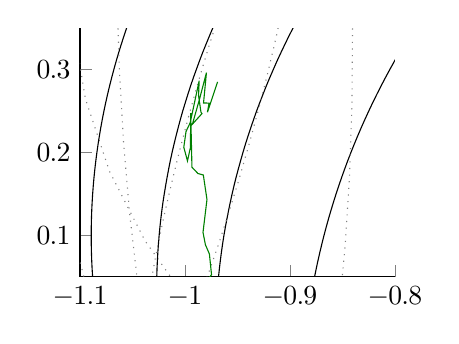
\begin{tikzpicture}

\begin{axis}[%
width=4cm,
height=3.15483870967742cm,
colormap={mymap}{[1pt] rgb(0pt)=(0,0,0); rgb(1pt)=(0,0,0)},
unbounded coords=jump,
scale only axis,
xmin=-1.1,
xmax=-0.8,
ymin=0.05,
ymax=0.35,
axis x line*=bottom,
axis y line*=left
]

\addplot[area legend,solid,draw=black,forget plot]
table[row sep=crcr]{
x y\\
-1.23 0.46490355595815 \\
-1.22960150659877 0.47 \\
-1.22869862032926 0.48 \\
-1.22767371065223 0.49 \\
-1.22652615959779 0.5 \\
-1.22525527442296 0.51 \\
-1.22386028691466 0.52 \\
-1.22234035261571 0.53 \\
-1.22069454997284 0.54 \\
-1.22 0.543925012252854 \\
-1.21892640279752 0.55 \\
-1.21703375996655 0.56 \\
-1.21501255351594 0.57 \\
-1.21286154858517 0.58 \\
-1.21057942808711 0.59 \\
-1.21 0.592406769213231 \\
-1.20817185045267 0.6 \\
-1.20563301512456 0.61 \\
-1.20295912720575 0.62 \\
-1.2001485327529 0.63 \\
-1.2 0.630505916752702 \\
-1.19720927177399 0.64 \\
-1.19413073501926 0.65 \\
-1.19091048235894 0.66 \\
-1.19 0.662717034143122 \\
-1.18755419286408 0.67 \\
-1.1840553713141 0.68 \\
-1.18040895669849 0.69 \\
-1.18 0.691082930921102 \\
-1.1766220430266 0.7 \\
-1.17268437715587 0.71 \\
-1.17 0.716574164360218 \\
-1.16859570678079 0.72 \\
-1.16435686868754 0.73 \\
-1.16 0.739906655398264 \\
-1.15995875610125 0.74 \\
-1.15540766506219 0.75 \\
-1.15069176174176 0.76 \\
-1.15 0.76142534514183 \\
-1.14581495754822 0.77 \\
-1.14076851906906 0.78 \\
-1.14 0.781481800290595 \\
-1.13555370431776 0.79 \\
-1.13016256518617 0.8 \\
-1.13 0.800294055571771 \\
-1.12459541368304 0.81 \\
-1.12 0.818003330802316 \\
-1.11884457213804 0.82 \\
-1.11290789864718 0.83 \\
-1.11 0.834766310779763 \\
-1.1067794262609 0.84 \\
-1.10045499989146 0.85 \\
-1.1 0.85070324293253 \\
-1.09392825155636 0.86 \\
-1.09 0.86585779537492 \\
-1.08719432959242 0.87 \\
-1.0802478170049 0.88 \\
-1.08 0.880349311626938 \\
-1.07307898957916 0.89 \\
-1.07 0.894191086141864 \\
-1.06568343026022 0.9 \\
-1.06 0.907472179329761 \\
-1.0580539964072 0.91 \\
-1.05018227493588 0.92 \\
-1.05 0.920227114822055 \\
-1.0420548844932 0.93 \\
-1.04 0.932474665837886 \\
-1.0336661072561 0.94 \\
-1.03 0.944267684379233 \\
-1.02500542583447 0.95 \\
-1.02 0.955632804221174 \\
-1.01606124067785 0.96 \\
-1.01 0.96659434215035 \\
-1.00682078403302 0.97 \\
-1 0.977174502586599 \\
-0.997270024404195 0.98 \\
-0.99 0.987393560386835 \\
-0.987393560386835 0.99 \\
-0.98 0.997270024404194 \\
-0.977174502586599 1 \\
-0.97 1.00682078403302 \\
-0.96659434215035 1.01 \\
-0.96 1.01606124067785 \\
-0.955632804221174 1.02 \\
-0.95 1.02500542583447 \\
-0.944267684379233 1.03 \\
-0.94 1.0336661072561 \\
-0.932474665837887 1.04 \\
-0.93 1.0420548844932 \\
-0.920227114822055 1.05 \\
-0.92 1.05018227493588 \\
-0.91 1.0580539964072 \\
-0.90747217932976 1.06 \\
-0.9 1.06568343026022 \\
-0.894191086141864 1.07 \\
-0.89 1.07307898957916 \\
-0.880349311626938 1.08 \\
-0.88 1.0802478170049 \\
-0.87 1.08719432959242 \\
-0.86585779537492 1.09 \\
-0.86 1.09392825155636 \\
-0.85070324293253 1.1 \\
-0.85 1.10045499989146 \\
-0.84 1.1067794262609 \\
-0.834766310779763 1.11 \\
-0.83 1.11290789864718 \\
-0.82 1.11884457213804 \\
-0.818003330802316 1.12 \\
-0.81 1.12459541368304 \\
-0.800294055571771 1.13 \\
-0.8 1.13016256518617 \\
-0.79 1.13555370431776 \\
-0.781481800290595 1.14 \\
-0.78 1.14076851906906 \\
-0.77 1.14581495754822 \\
-0.76142534514183 1.15 \\
-0.76 1.15069176174176 \\
-0.75 1.15540766506219 \\
-0.74 1.15995875610125 \\
-0.739906655398264 1.16 \\
-0.73 1.16435686868754 \\
-0.72 1.16859570678079 \\
-0.716574164360217 1.17 \\
-0.71 1.17268437715587 \\
-0.7 1.1766220430266 \\
-0.691082930921101 1.18 \\
-0.69 1.18040895669849 \\
-0.68 1.1840553713141 \\
-0.67 1.18755419286408 \\
-0.662717034143123 1.19 \\
-0.66 1.19091048235894 \\
-0.65 1.19413073501926 \\
-0.64 1.19720927177399 \\
-0.630505916752703 1.2 \\
-0.63 1.2001485327529 \\
-0.62 1.20295912720575 \\
-0.61 1.20563301512456 \\
-0.6 1.20817185045267 \\
-0.592406769213231 1.21 \\
-0.59 1.21057942808711 \\
-0.58 1.21286154858517 \\
-0.57 1.21501255351594 \\
-0.56 1.21703375996655 \\
-0.55 1.21892640279752 \\
-0.543925012252854 1.22 \\
-0.54 1.22069454997284 \\
-0.53 1.22234035261571 \\
-0.52 1.22386028691466 \\
-0.51 1.22525527442296 \\
-0.5 1.22652615959779 \\
-0.49 1.22767371065223 \\
-0.48 1.22869862032926 \\
-0.47 1.22960150659877 \\
-0.46490355595815 1.23 \\
-0.46 1.23038466003635 \\
-0.45 1.23104806991097 \\
-0.44 1.23159031728077 \\
-0.43 1.23201172796599 \\
-0.42 1.23231255504488 \\
-0.41 1.23249297910695 \\
-0.4 1.2325531084337 \\
-0.39 1.23249297910695 \\
-0.38 1.23231255504488 \\
-0.37 1.23201172796599 \\
-0.36 1.23159031728077 \\
-0.35 1.23104806991097 \\
-0.34 1.23038466003635 \\
-0.335096444041851 1.23 \\
-0.33 1.22960150659877 \\
-0.32 1.22869862032926 \\
-0.31 1.22767371065223 \\
-0.3 1.22652615959779 \\
-0.29 1.22525527442296 \\
-0.28 1.22386028691466 \\
-0.27 1.22234035261571 \\
-0.26 1.22069454997284 \\
-0.256074987747147 1.22 \\
-0.25 1.21892640279752 \\
-0.24 1.21703375996655 \\
-0.23 1.21501255351594 \\
-0.22 1.21286154858517 \\
-0.21 1.21057942808711 \\
-0.207593230786769 1.21 \\
-0.2 1.20817185045267 \\
-0.19 1.20563301512456 \\
-0.18 1.20295912720575 \\
-0.17 1.2001485327529 \\
-0.169494083247298 1.2 \\
-0.16 1.19720927177399 \\
-0.15 1.19413073501926 \\
-0.14 1.19091048235894 \\
-0.137282965856877 1.19 \\
-0.13 1.18755419286408 \\
-0.12 1.1840553713141 \\
-0.11 1.18040895669849 \\
-0.108917069078899 1.18 \\
-0.0999999999999999 1.1766220430266 \\
-0.0899999999999999 1.17268437715587 \\
-0.0834258356397825 1.17 \\
-0.0800000000000001 1.16859570678079 \\
-0.0700000000000001 1.16435686868754 \\
-0.0600933446017362 1.16 \\
-0.0600000000000001 1.15995875610125 \\
-0.05 1.15540766506219 \\
-0.04 1.15069176174176 \\
-0.0385746548581699 1.15 \\
-0.03 1.14581495754822 \\
-0.02 1.14076851906906 \\
-0.0185181997094054 1.14 \\
-0.01 1.13555370431776 \\
0 1.13016256518617 \\
0.000294055571771424 1.13 \\
0.01 1.12459541368304 \\
0.0180033308023158 1.12 \\
0.02 1.11884457213804 \\
0.03 1.11290789864718 \\
0.0347663107797624 1.11 \\
0.04 1.1067794262609 \\
0.05 1.10045499989146 \\
0.0507032429325301 1.1 \\
0.0600000000000001 1.09392825155636 \\
0.0658577953749194 1.09 \\
0.0700000000000001 1.08719432959242 \\
0.0800000000000001 1.0802478170049 \\
0.0803493116269377 1.08 \\
0.0899999999999999 1.07307898957916 \\
0.0941910861418636 1.07 \\
0.0999999999999999 1.06568343026022 \\
0.10747217932976 1.06 \\
0.11 1.0580539964072 \\
0.12 1.05018227493588 \\
0.120227114822055 1.05 \\
0.13 1.0420548844932 \\
0.132474665837886 1.04 \\
0.14 1.0336661072561 \\
0.144267684379233 1.03 \\
0.15 1.02500542583447 \\
0.155632804221174 1.02 \\
0.16 1.01606124067785 \\
0.16659434215035 1.01 \\
0.17 1.00682078403302 \\
0.1771745025866 1 \\
0.18 0.997270024404194 \\
0.187393560386835 0.99 \\
0.19 0.987393560386835 \\
0.197270024404195 0.98 \\
0.2 0.977174502586599 \\
0.206820784033018 0.97 \\
0.21 0.96659434215035 \\
0.216061240677853 0.96 \\
0.22 0.955632804221174 \\
0.225005425834474 0.95 \\
0.23 0.944267684379233 \\
0.233666107256098 0.94 \\
0.24 0.932474665837886 \\
0.242054884493204 0.93 \\
0.25 0.920227114822055 \\
0.250182274935881 0.92 \\
0.258053996407202 0.91 \\
0.26 0.907472179329761 \\
0.265683430260224 0.9 \\
0.27 0.894191086141863 \\
0.273078989579159 0.89 \\
0.28 0.880349311626938 \\
0.280247817004903 0.88 \\
0.287194329592418 0.87 \\
0.29 0.865857795374919 \\
0.293928251556358 0.86 \\
0.3 0.85070324293253 \\
0.300454999891464 0.85 \\
0.306779426260899 0.84 \\
0.31 0.834766310779762 \\
0.312907898647181 0.83 \\
0.318844572138043 0.82 \\
0.32 0.818003330802316 \\
0.324595413683044 0.81 \\
0.33 0.800294055571771 \\
0.330162565186173 0.8 \\
0.335553704317761 0.79 \\
0.34 0.781481800290595 \\
0.340768519069056 0.78 \\
0.345814957548218 0.77 \\
0.35 0.76142534514183 \\
0.350691761741762 0.76 \\
0.355407665062195 0.75 \\
0.359958756101252 0.74 \\
0.36 0.739906655398264 \\
0.364356868687543 0.73 \\
0.368595706780788 0.72 \\
0.37 0.716574164360218 \\
0.372684377155872 0.71 \\
0.376622043026596 0.7 \\
0.38 0.691082930921102 \\
0.380408956698492 0.69 \\
0.384055371314095 0.68 \\
0.387554192864077 0.67 \\
0.39 0.662717034143122 \\
0.390910482358941 0.66 \\
0.394130735019259 0.65 \\
0.397209271773994 0.64 \\
0.4 0.630505916752702 \\
0.400148532752897 0.63 \\
0.402959127205753 0.62 \\
0.405633015124562 0.61 \\
0.408171850452672 0.6 \\
0.41 0.592406769213231 \\
0.410579428087114 0.59 \\
0.41286154858517 0.58 \\
0.415012553515935 0.57 \\
0.417033759966547 0.56 \\
0.418926402797516 0.55 \\
0.42 0.543925012252854 \\
0.420694549972838 0.54 \\
0.422340352615714 0.53 \\
0.423860286914664 0.52 \\
0.425255274422965 0.51 \\
0.426526159597789 0.5 \\
0.427673710652226 0.49 \\
0.428698620329256 0.48 \\
0.429601506598767 0.47 \\
0.43 0.46490355595815 \\
0.430384660036347 0.46 \\
0.431048069910975 0.45 \\
0.431590317280767 0.44 \\
0.432011727965991 0.43 \\
0.432312555044877 0.42 \\
0.432492979106945 0.41 \\
0.432553108433699 0.4 \\
0.432492979106945 0.39 \\
0.432312555044877 0.38 \\
0.432011727965991 0.37 \\
0.431590317280767 0.36 \\
0.431048069910975 0.35 \\
0.430384660036347 0.34 \\
0.43 0.335096444041851 \\
0.429601506598767 0.33 \\
0.428698620329256 0.32 \\
0.427673710652226 0.31 \\
0.426526159597789 0.3 \\
0.425255274422965 0.29 \\
0.423860286914664 0.28 \\
0.422340352615714 0.27 \\
0.420694549972838 0.26 \\
0.42 0.256074987747147 \\
0.418926402797516 0.25 \\
0.417033759966547 0.24 \\
0.415012553515935 0.23 \\
0.41286154858517 0.22 \\
0.410579428087114 0.21 \\
0.41 0.207593230786769 \\
0.408171850452672 0.2 \\
0.405633015124562 0.19 \\
0.402959127205753 0.18 \\
0.400148532752897 0.17 \\
0.4 0.169494083247298 \\
0.397209271773994 0.16 \\
0.394130735019258 0.15 \\
0.390910482358941 0.14 \\
0.39 0.137282965856877 \\
0.387554192864077 0.13 \\
0.384055371314095 0.12 \\
0.380408956698492 0.11 \\
0.38 0.108917069078899 \\
0.376622043026596 0.0999999999999999 \\
0.372684377155872 0.0899999999999999 \\
0.37 0.0834258356397825 \\
0.368595706780788 0.0800000000000001 \\
0.364356868687543 0.0700000000000001 \\
0.36 0.0600933446017357 \\
0.359958756101252 0.0600000000000001 \\
0.355407665062195 0.05 \\
0.350691761741762 0.04 \\
0.35 0.0385746548581699 \\
0.345814957548218 0.03 \\
0.340768519069056 0.02 \\
0.34 0.0185181997094054 \\
0.335553704317761 0.01 \\
0.330162565186173 0 \\
0.33 -0.000294055571771139 \\
0.324595413683044 -0.01 \\
0.32 -0.0180033308023158 \\
0.318844572138043 -0.02 \\
0.312907898647181 -0.03 \\
0.31 -0.0347663107797621 \\
0.306779426260899 -0.04 \\
0.300454999891464 -0.05 \\
0.3 -0.0507032429325301 \\
0.293928251556357 -0.0600000000000001 \\
0.29 -0.0658577953749191 \\
0.287194329592418 -0.0700000000000001 \\
0.280247817004903 -0.0800000000000001 \\
0.28 -0.0803493116269377 \\
0.273078989579159 -0.0899999999999999 \\
0.27 -0.0941910861418633 \\
0.265683430260224 -0.0999999999999999 \\
0.26 -0.10747217932976 \\
0.258053996407202 -0.11 \\
0.250182274935881 -0.12 \\
0.25 -0.120227114822055 \\
0.242054884493204 -0.13 \\
0.24 -0.132474665837886 \\
0.233666107256098 -0.14 \\
0.23 -0.144267684379233 \\
0.225005425834474 -0.15 \\
0.22 -0.155632804221174 \\
0.216061240677853 -0.16 \\
0.21 -0.16659434215035 \\
0.206820784033018 -0.17 \\
0.2 -0.1771745025866 \\
0.197270024404195 -0.18 \\
0.19 -0.187393560386835 \\
0.187393560386835 -0.19 \\
0.18 -0.197270024404195 \\
0.1771745025866 -0.2 \\
0.17 -0.206820784033018 \\
0.16659434215035 -0.21 \\
0.16 -0.216061240677853 \\
0.155632804221174 -0.22 \\
0.15 -0.225005425834474 \\
0.144267684379233 -0.23 \\
0.14 -0.233666107256098 \\
0.132474665837886 -0.24 \\
0.13 -0.242054884493204 \\
0.120227114822055 -0.25 \\
0.12 -0.250182274935881 \\
0.11 -0.258053996407202 \\
0.10747217932976 -0.26 \\
0.0999999999999999 -0.265683430260224 \\
0.0941910861418633 -0.27 \\
0.0899999999999999 -0.273078989579159 \\
0.0803493116269377 -0.28 \\
0.0800000000000001 -0.280247817004903 \\
0.0700000000000001 -0.287194329592418 \\
0.0658577953749191 -0.29 \\
0.0600000000000001 -0.293928251556357 \\
0.0507032429325301 -0.3 \\
0.05 -0.300454999891464 \\
0.04 -0.306779426260899 \\
0.0347663107797621 -0.31 \\
0.03 -0.312907898647181 \\
0.02 -0.318844572138043 \\
0.0180033308023158 -0.32 \\
0.01 -0.324595413683044 \\
0.000294055571771139 -0.33 \\
0 -0.330162565186173 \\
-0.01 -0.335553704317761 \\
-0.0185181997094054 -0.34 \\
-0.02 -0.340768519069056 \\
-0.03 -0.345814957548218 \\
-0.0385746548581699 -0.35 \\
-0.04 -0.350691761741762 \\
-0.05 -0.355407665062195 \\
-0.0600000000000001 -0.359958756101252 \\
-0.0600933446017357 -0.36 \\
-0.0700000000000001 -0.364356868687543 \\
-0.0800000000000001 -0.368595706780788 \\
-0.0834258356397825 -0.37 \\
-0.0899999999999999 -0.372684377155872 \\
-0.0999999999999999 -0.376622043026596 \\
-0.108917069078899 -0.38 \\
-0.11 -0.380408956698492 \\
-0.12 -0.384055371314095 \\
-0.13 -0.387554192864077 \\
-0.137282965856877 -0.39 \\
-0.14 -0.390910482358941 \\
-0.15 -0.394130735019258 \\
-0.16 -0.397209271773994 \\
-0.169494083247298 -0.4 \\
-0.17 -0.400148532752897 \\
-0.18 -0.402959127205753 \\
-0.19 -0.405633015124562 \\
-0.2 -0.408171850452672 \\
-0.207593230786769 -0.41 \\
-0.21 -0.410579428087114 \\
-0.22 -0.41286154858517 \\
-0.23 -0.415012553515935 \\
-0.24 -0.417033759966547 \\
-0.25 -0.418926402797516 \\
-0.256074987747147 -0.42 \\
-0.26 -0.420694549972838 \\
-0.27 -0.422340352615714 \\
-0.28 -0.423860286914664 \\
-0.29 -0.425255274422965 \\
-0.3 -0.426526159597789 \\
-0.31 -0.427673710652226 \\
-0.32 -0.428698620329256 \\
-0.33 -0.429601506598767 \\
-0.335096444041851 -0.43 \\
-0.34 -0.430384660036347 \\
-0.35 -0.431048069910975 \\
-0.36 -0.431590317280767 \\
-0.37 -0.432011727965991 \\
-0.38 -0.432312555044877 \\
-0.39 -0.432492979106945 \\
-0.4 -0.432553108433699 \\
-0.41 -0.432492979106945 \\
-0.42 -0.432312555044877 \\
-0.43 -0.432011727965991 \\
-0.44 -0.431590317280767 \\
-0.45 -0.431048069910975 \\
-0.46 -0.430384660036347 \\
-0.46490355595815 -0.43 \\
-0.47 -0.429601506598767 \\
-0.48 -0.428698620329256 \\
-0.49 -0.427673710652226 \\
-0.5 -0.426526159597789 \\
-0.51 -0.425255274422965 \\
-0.52 -0.423860286914664 \\
-0.53 -0.422340352615714 \\
-0.54 -0.420694549972838 \\
-0.543925012252854 -0.42 \\
-0.55 -0.418926402797516 \\
-0.56 -0.417033759966547 \\
-0.57 -0.415012553515935 \\
-0.58 -0.41286154858517 \\
-0.59 -0.410579428087114 \\
-0.592406769213231 -0.41 \\
-0.6 -0.408171850452672 \\
-0.61 -0.405633015124562 \\
-0.62 -0.402959127205753 \\
-0.63 -0.400148532752897 \\
-0.630505916752703 -0.4 \\
-0.64 -0.397209271773994 \\
-0.65 -0.394130735019259 \\
-0.66 -0.390910482358941 \\
-0.662717034143123 -0.39 \\
-0.67 -0.387554192864077 \\
-0.68 -0.384055371314095 \\
-0.69 -0.380408956698492 \\
-0.691082930921101 -0.38 \\
-0.7 -0.376622043026596 \\
-0.71 -0.372684377155872 \\
-0.716574164360217 -0.37 \\
-0.72 -0.368595706780788 \\
-0.73 -0.364356868687543 \\
-0.739906655398264 -0.36 \\
-0.74 -0.359958756101252 \\
-0.75 -0.355407665062195 \\
-0.76 -0.350691761741762 \\
-0.76142534514183 -0.35 \\
-0.77 -0.345814957548218 \\
-0.78 -0.340768519069056 \\
-0.781481800290595 -0.34 \\
-0.79 -0.335553704317761 \\
-0.8 -0.330162565186173 \\
-0.800294055571771 -0.33 \\
-0.81 -0.324595413683044 \\
-0.818003330802316 -0.32 \\
-0.82 -0.318844572138043 \\
-0.83 -0.312907898647181 \\
-0.834766310779762 -0.31 \\
-0.84 -0.306779426260899 \\
-0.85 -0.300454999891464 \\
-0.85070324293253 -0.3 \\
-0.86 -0.293928251556358 \\
-0.865857795374919 -0.29 \\
-0.87 -0.287194329592418 \\
-0.88 -0.280247817004903 \\
-0.880349311626938 -0.28 \\
-0.89 -0.273078989579159 \\
-0.894191086141863 -0.27 \\
-0.9 -0.265683430260224 \\
-0.90747217932976 -0.26 \\
-0.91 -0.258053996407202 \\
-0.92 -0.250182274935881 \\
-0.920227114822055 -0.25 \\
-0.93 -0.242054884493204 \\
-0.932474665837887 -0.24 \\
-0.94 -0.233666107256098 \\
-0.944267684379233 -0.23 \\
-0.95 -0.225005425834474 \\
-0.955632804221174 -0.22 \\
-0.96 -0.216061240677853 \\
-0.96659434215035 -0.21 \\
-0.97 -0.206820784033018 \\
-0.977174502586599 -0.2 \\
-0.98 -0.197270024404195 \\
-0.987393560386835 -0.19 \\
-0.99 -0.187393560386835 \\
-0.997270024404195 -0.18 \\
-1 -0.1771745025866 \\
-1.00682078403302 -0.17 \\
-1.01 -0.16659434215035 \\
-1.01606124067785 -0.16 \\
-1.02 -0.155632804221174 \\
-1.02500542583447 -0.15 \\
-1.03 -0.144267684379233 \\
-1.0336661072561 -0.14 \\
-1.04 -0.132474665837886 \\
-1.0420548844932 -0.13 \\
-1.05 -0.120227114822055 \\
-1.05018227493588 -0.12 \\
-1.0580539964072 -0.11 \\
-1.06 -0.10747217932976 \\
-1.06568343026022 -0.0999999999999999 \\
-1.07 -0.0941910861418636 \\
-1.07307898957916 -0.0899999999999999 \\
-1.08 -0.0803493116269377 \\
-1.0802478170049 -0.0800000000000001 \\
-1.08719432959242 -0.0700000000000001 \\
-1.09 -0.0658577953749194 \\
-1.09392825155636 -0.0600000000000001 \\
-1.1 -0.0507032429325301 \\
-1.10045499989146 -0.05 \\
-1.1067794262609 -0.04 \\
-1.11 -0.0347663107797624 \\
-1.11290789864718 -0.03 \\
-1.11884457213804 -0.02 \\
-1.12 -0.0180033308023158 \\
-1.12459541368304 -0.01 \\
-1.13 -0.000294055571771424 \\
-1.13016256518617 0 \\
-1.13555370431776 0.01 \\
-1.14 0.0185181997094054 \\
-1.14076851906906 0.02 \\
-1.14581495754822 0.03 \\
-1.15 0.0385746548581699 \\
-1.15069176174176 0.04 \\
-1.15540766506219 0.05 \\
-1.15995875610125 0.0600000000000001 \\
-1.16 0.0600933446017362 \\
-1.16435686868754 0.0700000000000001 \\
-1.16859570678079 0.0800000000000001 \\
-1.17 0.0834258356397825 \\
-1.17268437715587 0.0899999999999999 \\
-1.1766220430266 0.0999999999999999 \\
-1.18 0.108917069078899 \\
-1.18040895669849 0.11 \\
-1.1840553713141 0.12 \\
-1.18755419286408 0.13 \\
-1.19 0.137282965856877 \\
-1.19091048235894 0.14 \\
-1.19413073501926 0.15 \\
-1.19720927177399 0.16 \\
-1.2 0.169494083247298 \\
-1.2001485327529 0.17 \\
-1.20295912720575 0.18 \\
-1.20563301512456 0.19 \\
-1.20817185045267 0.2 \\
-1.21 0.207593230786769 \\
-1.21057942808711 0.21 \\
-1.21286154858517 0.22 \\
-1.21501255351594 0.23 \\
-1.21703375996655 0.24 \\
-1.21892640279752 0.25 \\
-1.22 0.256074987747147 \\
-1.22069454997284 0.26 \\
-1.22234035261571 0.27 \\
-1.22386028691466 0.28 \\
-1.22525527442296 0.29 \\
-1.22652615959779 0.3 \\
-1.22767371065223 0.31 \\
-1.22869862032926 0.32 \\
-1.22960150659877 0.33 \\
-1.23 0.335096444041851 \\
-1.23038466003635 0.34 \\
-1.23104806991097 0.35 \\
-1.23159031728077 0.36 \\
-1.23201172796599 0.37 \\
-1.23231255504488 0.38 \\
-1.23249297910694 0.39 \\
-1.2325531084337 0.4 \\
-1.23249297910694 0.41 \\
-1.23231255504488 0.42 \\
-1.23201172796599 0.43 \\
-1.23159031728077 0.44 \\
-1.23104806991097 0.45 \\
-1.23038466003635 0.46 \\
-1.23 0.46490355595815 \\
NaN NaN \\
};

\addplot [
color=gray,
dotted,
forget plot
]
table[row sep=crcr]{
0.302858053669543 0.4\\
0.29706717591351 0.490422808186003\\
0.279789628698068 0.579360876361465\\
0.25130910887083 0.665353843905771\\
0.212093265779973 0.746989708669247\\
0.162786022484869 0.822928012009422\\
0.104197002557251 0.891921849084879\\
0.0372882360845491 0.952838342998275\\
-0.0368416368375469 1.00467724660368\\
-0.116975405745088 1.04658736653706\\
-0.201797276368028 1.07788053978777\\
-0.289914475935768 1.09804293331619\\
-0.379880122467536 1.10674348117799\\
-0.470216982534515 1.10383932061783\\
-0.559441727391902 1.08937813787181\\
-0.64608928919589 1.06359738516082\\
-0.72873691737716 1.02692038173164\\
-0.806027540165891 0.979949362966567\\
-0.876692047672707 0.923455591695151\\
-0.939570130637972 0.858366694079811\\
-0.993629332677755 0.785751428019912\\
-1.03798200318911 0.7068021341766\\
-1.07189987254844 0.622815157772112\\
-1.09482601027856 0.535169562637062\\
-1.10638396983179 0.445304487020476\\
-1.10638396983179 0.354695512979524\\
-1.09482601027856 0.264830437362938\\
-1.07189987254844 0.177184842227889\\
-1.03798200318911 0.0931978658233998\\
-0.993629332677756 0.0142485719800879\\
-0.939570130637972 -0.058366694079811\\
-0.876692047672707 -0.123455591695151\\
-0.806027540165891 -0.179949362966567\\
-0.72873691737716 -0.226920381731638\\
-0.64608928919589 -0.263597385160825\\
-0.559441727391902 -0.28937813787181\\
-0.470216982534514 -0.303839320617828\\
-0.379880122467536 -0.30674348117799\\
-0.289914475935769 -0.298042933316187\\
-0.201797276368029 -0.277880539787771\\
-0.116975405745088 -0.246587366537059\\
-0.0368416368375474 -0.204677246603681\\
0.037288236084549 -0.152838342998275\\
0.10419700255725 -0.0919218490848791\\
0.162786022484868 -0.0229280120094228\\
0.212093265779973 0.0530102913307532\\
0.25130910887083 0.134646156094229\\
0.279789628698068 0.220639123638535\\
0.29706717591351 0.309577191813997\\
0.302858053669543 0.4\\
};

\addplot[area legend,solid,draw=black,forget plot]
table[row sep=crcr]{
x y\\
-1.17 0.34824483234669 \\
-1.16974685063192 0.35 \\
-1.16819226362119 0.36 \\
-1.16652579083749 0.37 \\
-1.16474640465062 0.38 \\
-1.16285290186727 0.39 \\
-1.16084389340103 0.4 \\
-1.16 0.403972283004096 \\
-1.15872752024962 0.41 \\
-1.15650161857746 0.42 \\
-1.15415850992452 0.43 \\
-1.15169620345948 0.44 \\
-1.15 0.446570497508841 \\
-1.14911957270876 0.45 \\
-1.14643582378503 0.46 \\
-1.14362995065294 0.47 \\
-1.14069920346947 0.48 \\
-1.14 0.482292669864651 \\
-1.13766087050511 0.49 \\
-1.13450203673762 0.5 \\
-1.13121376409444 0.51 \\
-1.13 0.513558350248353 \\
-1.1278116203584 0.52 \\
-1.12428796612075 0.53 \\
-1.12062893201116 0.54 \\
-1.12 0.541663477723823 \\
-1.11685840800488 0.55 \\
-1.11295502020046 0.56 \\
-1.11 0.56731503463497 \\
-1.1089179667055 0.57 \\
-1.10476285025168 0.58 \\
-1.10046101620946 0.59 \\
-1.1 0.591041770839401 \\
-1.09604227319328 0.6 \\
-1.09147623443274 0.61 \\
-1.09 0.613142166756836 \\
-1.08678076273977 0.62 \\
-1.08194080954232 0.63 \\
-1.08 0.633899158806308 \\
-1.07696335112985 0.64 \\
-1.07183867003779 0.65 \\
-1.07 0.653493256137173 \\
-1.06657249843507 0.66 \\
-1.06115098587887 0.67 \\
-1.06 0.672071557680547 \\
-1.05558789116181 0.68 \\
-1.05 0.689751052742826 \\
-1.04985699636204 0.69 \\
-1.04398616547374 0.7 \\
-1.04 0.706603959589081 \\
-1.03794361838801 0.71 \\
-1.03174054970386 0.72 \\
-1.03 0.722741706044418 \\
-1.02537385112673 0.73 \\
-1.02 0.738216777058695 \\
-1.01882821800339 0.74 \\
-1.01211523648097 0.75 \\
-1.01 0.753080756290404 \\
-1.00522296955145 0.76 \\
-1 0.767388077842723 \\
-0.998141887321532 0.77 \\
-0.990874145928976 0.78 \\
-0.99 0.781179799014672 \\
-0.983418455088601 0.79 \\
-0.98 0.794483082457343 \\
-0.975760203119438 0.8 \\
-0.97 0.807340585135123 \\
-0.967895220180388 0.81 \\
-0.96 0.819777404251693 \\
-0.959818579796784 0.82 \\
-0.951530102936964 0.83 \\
-0.95 0.831812067722366 \\
-0.943015865809287 0.84 \\
-0.94 0.843472184497663 \\
-0.934268290314526 0.85 \\
-0.93 0.854777416654995 \\
-0.925279730157293 0.86 \\
-0.92 0.865745241610559 \\
-0.916041674018024 0.87 \\
-0.91 0.876391723329543 \\
-0.906544708951422 0.88 \\
-0.9 0.886731619659182 \\
-0.896778476336056 0.89 \\
-0.89 0.896778476336056 \\
-0.886731619659182 0.9 \\
-0.88 0.906544708951422 \\
-0.876391723329543 0.91 \\
-0.87 0.916041674018024 \\
-0.865745241610559 0.92 \\
-0.86 0.925279730157293 \\
-0.854777416654995 0.93 \\
-0.85 0.934268290314526 \\
-0.843472184497663 0.94 \\
-0.84 0.943015865809288 \\
-0.831812067722366 0.95 \\
-0.83 0.951530102936965 \\
-0.82 0.959818579796784 \\
-0.819777404251693 0.96 \\
-0.81 0.967895220180388 \\
-0.807340585135122 0.97 \\
-0.8 0.975760203119437 \\
-0.794483082457343 0.98 \\
-0.79 0.983418455088602 \\
-0.781179799014672 0.99 \\
-0.78 0.990874145928976 \\
-0.77 0.998141887321532 \\
-0.767388077842723 1 \\
-0.76 1.00522296955145 \\
-0.753080756290404 1.01 \\
-0.75 1.01211523648097 \\
-0.74 1.01882821800339 \\
-0.738216777058696 1.02 \\
-0.73 1.02537385112673 \\
-0.722741706044418 1.03 \\
-0.72 1.03174054970386 \\
-0.71 1.03794361838801 \\
-0.706603959589081 1.04 \\
-0.7 1.04398616547375 \\
-0.69 1.04985699636204 \\
-0.689751052742826 1.05 \\
-0.68 1.05558789116181 \\
-0.672071557680547 1.06 \\
-0.67 1.06115098587887 \\
-0.66 1.06657249843507 \\
-0.653493256137172 1.07 \\
-0.65 1.07183867003779 \\
-0.64 1.07696335112985 \\
-0.633899158806308 1.08 \\
-0.63 1.08194080954232 \\
-0.62 1.08678076273977 \\
-0.613142166756836 1.09 \\
-0.61 1.09147623443274 \\
-0.6 1.09604227319328 \\
-0.591041770839401 1.1 \\
-0.59 1.10046101620946 \\
-0.58 1.10476285025168 \\
-0.57 1.1089179667055 \\
-0.56731503463497 1.11 \\
-0.56 1.11295502020045 \\
-0.55 1.11685840800488 \\
-0.541663477723823 1.12 \\
-0.54 1.12062893201116 \\
-0.53 1.12428796612075 \\
-0.52 1.1278116203584 \\
-0.513558350248353 1.13 \\
-0.51 1.13121376409444 \\
-0.5 1.13450203673762 \\
-0.49 1.13766087050511 \\
-0.482292669864651 1.14 \\
-0.48 1.14069920346947 \\
-0.47 1.14362995065294 \\
-0.46 1.14643582378503 \\
-0.45 1.14911957270876 \\
-0.446570497508841 1.15 \\
-0.44 1.15169620345948 \\
-0.43 1.15415850992452 \\
-0.42 1.15650161857746 \\
-0.41 1.15872752024962 \\
-0.403972283004096 1.16 \\
-0.4 1.16084389340103 \\
-0.39 1.16285290186727 \\
-0.38 1.16474640465062 \\
-0.37 1.16652579083749 \\
-0.36 1.16819226362119 \\
-0.35 1.16974685063192 \\
-0.34824483234669 1.17 \\
-0.34 1.17119736332875 \\
-0.33 1.17253708306572 \\
-0.32 1.17376516554583 \\
-0.31 1.17488223536639 \\
-0.3 1.17588878364361 \\
-0.29 1.17678517647896 \\
-0.28 1.17757166314514 \\
-0.27 1.17824838400104 \\
-0.26 1.17881537814023 \\
-0.25 1.17927259077445 \\
-0.24 1.17961988034923 \\
-0.23 1.1798570253855 \\
-0.22 1.17998373103776 \\
-0.21 1.17999963535578 \\
-0.2 1.17990431523439 \\
-0.19 1.17969729203277 \\
-0.18 1.17937803684251 \\
-0.17 1.17894597538143 \\
-0.16 1.17840049248854 \\
-0.15 1.17774093619399 \\
-0.14 1.1769666213368 \\
-0.13 1.17607683270263 \\
-0.12 1.17507082765349 \\
-0.11 1.17394783822133 \\
-0.0999999999999999 1.17270707263833 \\
-0.0899999999999999 1.17134771627709 \\
-0.0808808221553111 1.17 \\
-0.0800000000000001 1.169868446055 \\
-0.0700000000000001 1.16826318492631 \\
-0.0600000000000001 1.1665358522753 \\
-0.05 1.16468558953898 \\
-0.04 1.16271152558355 \\
-0.03 1.16061277372685 \\
-0.0272297162274458 1.16 \\
-0.02 1.15837707043464 \\
-0.01 1.15600950424899 \\
0 1.15351353518583 \\
0.01 1.15088831903331 \\
0.0132417961451759 1.15 \\
0.02 1.1481144843506 \\
0.03 1.1451998014171 \\
0.04 1.14215236860539 \\
0.0467845809778874 1.14 \\
0.05 1.13895839590464 \\
0.0600000000000001 1.13560172760492 \\
0.0700000000000001 1.13210924568362 \\
0.0758326192762357 1.13 \\
0.0800000000000001 1.12845705211644 \\
0.0899999999999999 1.12463447377779 \\
0.0999999999999999 1.12067372352401 \\
0.101654875861228 1.12 \\
0.11 1.11651329321956 \\
0.12 1.11220142977958 \\
0.124965625555616 1.11 \\
0.13 1.10770379085866 \\
0.14 1.10302068977659 \\
0.146281627658991 1.1 \\
0.15 1.09815606221167 \\
0.16 1.09308122969512 \\
0.165927999060679 1.09 \\
0.17 1.08781244454026 \\
0.18 1.08232554760214 \\
0.18415237085094 1.08 \\
0.19 1.07660791404929 \\
0.2 1.07068940384791 \\
0.201145721652617 1.07 \\
0.21 1.06447069599288 \\
0.217032177449418 1.06 \\
0.22 1.05803665457619 \\
0.23 1.05132313374821 \\
0.231943882101265 1.05 \\
0.24 1.04428372571177 \\
0.245958520328016 1.04 \\
0.25 1.03696310983243 \\
0.259164215758356 1.03 \\
0.26 1.02933444169534 \\
0.27 1.02130039326315 \\
0.27160451321306 1.02 \\
0.28 1.01285817275248 \\
0.283336244087455 1.01 \\
0.29 1.0039916294524 \\
0.29440365869371 1 \\
0.3 0.994646303613179 \\
0.30483949801983 0.99 \\
0.31 0.984756110397065 \\
0.314671396184423 0.98 \\
0.32 0.974240900702571 \\
0.323922474439262 0.97 \\
0.33 0.963003381220004 \\
0.332611869145027 0.96 \\
0.34 0.950925197880764 \\
0.340755206485876 0.95 \\
0.348353919103909 0.94 \\
0.35 0.937660090845779 \\
0.355419004395882 0.93 \\
0.36 0.922984220900905 \\
0.361962087595305 0.92 \\
0.36797165252887 0.91 \\
0.37 0.906270424491979 \\
0.373443745141697 0.9 \\
0.378378429548447 0.89 \\
0.38 0.8862599122459 \\
0.382748545988888 0.88 \\
0.386543456781287 0.87 \\
0.389749012796172 0.86 \\
0.39 0.859001026024989 \\
0.392300698766757 0.85 \\
0.394180890645867 0.84 \\
0.395336251754202 0.83 \\
0.395697015250948 0.82 \\
0.395176614410703 0.81 \\
0.39366754926419 0.8 \\
0.391035889986567 0.79 \\
0.39 0.787258661419913 \\
0.38705697916176 0.78 \\
0.381513307702241 0.77 \\
0.38 0.76784594377993 \\
0.374007445086244 0.76 \\
0.37 0.7557514351253 \\
0.364054295499889 0.75 \\
0.36 0.746700822030463 \\
0.350894547332186 0.74 \\
0.35 0.739430738915723 \\
0.34 0.733546956944958 \\
0.333298499271874 0.73 \\
0.33 0.728449374871357 \\
0.32 0.724105387704512 \\
0.31 0.720189628818945 \\
0.30948537538196 0.72 \\
0.3 0.716820146879085 \\
0.29 0.713742733243921 \\
0.28 0.710905686344939 \\
0.276631981808553 0.71 \\
0.27 0.708348249786546 \\
0.26 0.705990225868927 \\
0.25 0.703765986162755 \\
0.24 0.701653387666864 \\
0.231856513506836 0.7 \\
0.23 0.699645189000129 \\
0.22 0.697762633450779 \\
0.21 0.695933040344062 \\
0.2 0.694143056983395 \\
0.19 0.692380555671002 \\
0.18 0.690634479159236 \\
0.176397789260313 0.69 \\
0.17 0.688922459583778 \\
0.16 0.687221648864136 \\
0.15 0.685507533384693 \\
0.14 0.683772550733038 \\
0.13 0.682009658682955 \\
0.12 0.680212272727076 \\
0.118859861177737 0.68 \\
0.11 0.678404402725216 \\
0.0999999999999999 0.676553533757192 \\
0.0899999999999999 0.674650364964621 \\
0.0800000000000001 0.672689883309064 \\
0.0700000000000001 0.670667299751165 \\
0.0668306100783585 0.67 \\
0.0600000000000001 0.668597853651372 \\
0.05 0.66646691237605 \\
0.04 0.664260949803104 \\
0.03 0.661976004677973 \\
0.0216673934388655 0.66 \\
0.02 0.659612293922447 \\
0.01 0.657183320094115 \\
0 0.65466475610035 \\
-0.01 0.652053104374175 \\
-0.017567454667616 0.65 \\
-0.02 0.649349850941758 \\
-0.03 0.646563140809441 \\
-0.04 0.643674188237087 \\
-0.05 0.640679674329226 \\
-0.052180207372021 0.64 \\
-0.0600000000000001 0.637589219183333 \\
-0.0700000000000001 0.63439166581964 \\
-0.0800000000000001 0.631080205491351 \\
-0.0831402257352855 0.63 \\
-0.0899999999999999 0.627659442913738 \\
-0.0999999999999999 0.624123550351529 \\
-0.11 0.620465748641229 \\
-0.111227012060718 0.62 \\
-0.12 0.616688410403288 \\
-0.13 0.612785488763925 \\
-0.136900064685736 0.61 \\
-0.14 0.60875277155352 \\
-0.15 0.604588741202766 \\
-0.16 0.600290571267089 \\
-0.16065351031315 0.6 \\
-0.17 0.595850011960966 \\
-0.18 0.591270707191558 \\
-0.182687213649655 0.59 \\
-0.19 0.586540695511637 \\
-0.2 0.581664556411378 \\
-0.203310270220351 0.58 \\
-0.21 0.576629475148341 \\
-0.22 0.571440830887073 \\
-0.222695730199283 0.57 \\
-0.23 0.566082636343688 \\
-0.24 0.56056576211472 \\
-0.240996536634055 0.56 \\
-0.25 0.554864283969042 \\
-0.25829823208705 0.55 \\
-0.26 0.548996397299665 \\
-0.27 0.542936451594461 \\
-0.274718974924906 0.54 \\
-0.28 0.53669018665601 \\
-0.29 0.530259090650918 \\
-0.290392682652562 0.53 \\
-0.3 0.523608996367508 \\
-0.305292522306472 0.52 \\
-0.31 0.516760031015857 \\
-0.31958736311537 0.51 \\
-0.32 0.509706038368183 \\
-0.33 0.502411592496721 \\
-0.333230504355639 0.5 \\
-0.34 0.494889881614602 \\
-0.346333666426978 0.49 \\
-0.35 0.487135070921797 \\
-0.358933405813462 0.48 \\
-0.36 0.479137028373567 \\
-0.37 0.470872491657892 \\
-0.371034071904004 0.47 \\
-0.38 0.462330832836047 \\
-0.382670783399685 0.46 \\
-0.39 0.45351036479971 \\
-0.393888241389502 0.45 \\
-0.4 0.444397399512695 \\
-0.404707850571412 0.44 \\
-0.41 0.434977128695799 \\
-0.415149914587216 0.43 \\
-0.42 0.425233637932722 \\
-0.425233637932722 0.42 \\
-0.43 0.415149914587216 \\
-0.434977128695799 0.41 \\
-0.44 0.404707850571412 \\
-0.444397399512695 0.4 \\
-0.45 0.393888241389502 \\
-0.45351036479971 0.39 \\
-0.46 0.382670783399685 \\
-0.462330832836047 0.38 \\
-0.47 0.371034071904004 \\
-0.470872491657892 0.37 \\
-0.479137028373567 0.36 \\
-0.48 0.358933405813462 \\
-0.487135070921797 0.35 \\
-0.49 0.346333666426978 \\
-0.494889881614602 0.34 \\
-0.5 0.333230504355639 \\
-0.502411592496721 0.33 \\
-0.509706038368183 0.32 \\
-0.51 0.31958736311537 \\
-0.516760031015857 0.31 \\
-0.52 0.305292522306472 \\
-0.523608996367508 0.3 \\
-0.53 0.290392682652562 \\
-0.530259090650918 0.29 \\
-0.53669018665601 0.28 \\
-0.54 0.274718974924906 \\
-0.542936451594461 0.27 \\
-0.548996397299665 0.26 \\
-0.55 0.25829823208705 \\
-0.554864283969042 0.25 \\
-0.56 0.240996536634055 \\
-0.560565762114719 0.24 \\
-0.566082636343688 0.23 \\
-0.57 0.222695730199283 \\
-0.571440830887073 0.22 \\
-0.576629475148341 0.21 \\
-0.58 0.203310270220351 \\
-0.581664556411378 0.2 \\
-0.586540695511637 0.19 \\
-0.59 0.182687213649655 \\
-0.591270707191558 0.18 \\
-0.595850011960966 0.17 \\
-0.6 0.16065351031315 \\
-0.600290571267089 0.16 \\
-0.604588741202766 0.15 \\
-0.60875277155352 0.14 \\
-0.61 0.136900064685736 \\
-0.612785488763925 0.13 \\
-0.616688410403289 0.12 \\
-0.62 0.111227012060718 \\
-0.620465748641228 0.11 \\
-0.624123550351529 0.0999999999999999 \\
-0.627659442913738 0.0899999999999999 \\
-0.63 0.0831402257352855 \\
-0.631080205491351 0.0800000000000001 \\
-0.63439166581964 0.0700000000000001 \\
-0.637589219183333 0.0600000000000001 \\
-0.64 0.052180207372021 \\
-0.640679674329226 0.05 \\
-0.643674188237087 0.04 \\
-0.64656314080944 0.03 \\
-0.649349850941758 0.02 \\
-0.65 0.017567454667616 \\
-0.652053104374176 0.01 \\
-0.654664756100351 0 \\
-0.657183320094115 -0.01 \\
-0.659612293922446 -0.02 \\
-0.66 -0.0216673934388655 \\
-0.661976004677973 -0.03 \\
-0.664260949803104 -0.04 \\
-0.66646691237605 -0.05 \\
-0.668597853651372 -0.0600000000000001 \\
-0.67 -0.0668306100783585 \\
-0.670667299751165 -0.0700000000000001 \\
-0.672689883309064 -0.0800000000000001 \\
-0.674650364964621 -0.0899999999999999 \\
-0.676553533757192 -0.0999999999999999 \\
-0.678404402725216 -0.11 \\
-0.68 -0.118859861177737 \\
-0.680212272727076 -0.12 \\
-0.682009658682955 -0.13 \\
-0.683772550733038 -0.14 \\
-0.685507533384693 -0.15 \\
-0.687221648864136 -0.16 \\
-0.688922459583777 -0.17 \\
-0.69 -0.176397789260313 \\
-0.690634479159236 -0.18 \\
-0.692380555671002 -0.19 \\
-0.694143056983395 -0.2 \\
-0.695933040344063 -0.21 \\
-0.697762633450779 -0.22 \\
-0.699645189000129 -0.23 \\
-0.7 -0.231856513506836 \\
-0.701653387666865 -0.24 \\
-0.703765986162755 -0.25 \\
-0.705990225868927 -0.26 \\
-0.708348249786546 -0.27 \\
-0.71 -0.276631981808553 \\
-0.71090568634494 -0.28 \\
-0.713742733243921 -0.29 \\
-0.716820146879085 -0.3 \\
-0.72 -0.30948537538196 \\
-0.720189628818945 -0.31 \\
-0.724105387704512 -0.32 \\
-0.728449374871357 -0.33 \\
-0.73 -0.333298499271874 \\
-0.733546956944958 -0.34 \\
-0.739430738915724 -0.35 \\
-0.74 -0.350894547332186 \\
-0.746700822030463 -0.36 \\
-0.75 -0.364054295499889 \\
-0.7557514351253 -0.37 \\
-0.76 -0.374007445086244 \\
-0.767845943779929 -0.38 \\
-0.77 -0.381513307702241 \\
-0.78 -0.38705697916176 \\
-0.787258661419913 -0.39 \\
-0.79 -0.391035889986567 \\
-0.8 -0.39366754926419 \\
-0.81 -0.395176614410703 \\
-0.82 -0.395697015250948 \\
-0.83 -0.395336251754202 \\
-0.84 -0.394180890645867 \\
-0.85 -0.392300698766757 \\
-0.859001026024989 -0.39 \\
-0.86 -0.389749012796172 \\
-0.87 -0.386543456781287 \\
-0.88 -0.382748545988888 \\
-0.8862599122459 -0.38 \\
-0.89 -0.378378429548447 \\
-0.9 -0.373443745141697 \\
-0.906270424491979 -0.37 \\
-0.91 -0.36797165252887 \\
-0.92 -0.361962087595305 \\
-0.922984220900905 -0.36 \\
-0.93 -0.355419004395882 \\
-0.93766009084578 -0.35 \\
-0.94 -0.348353919103909 \\
-0.95 -0.340755206485876 \\
-0.950925197880764 -0.34 \\
-0.96 -0.332611869145027 \\
-0.963003381220003 -0.33 \\
-0.97 -0.323922474439262 \\
-0.974240900702571 -0.32 \\
-0.98 -0.314671396184423 \\
-0.984756110397065 -0.31 \\
-0.99 -0.30483949801983 \\
-0.994646303613179 -0.3 \\
-1 -0.29440365869371 \\
-1.0039916294524 -0.29 \\
-1.01 -0.283336244087455 \\
-1.01285817275248 -0.28 \\
-1.02 -0.27160451321306 \\
-1.02130039326315 -0.27 \\
-1.02933444169534 -0.26 \\
-1.03 -0.259164215758356 \\
-1.03696310983243 -0.25 \\
-1.04 -0.245958520328016 \\
-1.04428372571177 -0.24 \\
-1.05 -0.231943882101265 \\
-1.05132313374821 -0.23 \\
-1.05803665457619 -0.22 \\
-1.06 -0.217032177449418 \\
-1.06447069599288 -0.21 \\
-1.07 -0.201145721652617 \\
-1.07068940384791 -0.2 \\
-1.07660791404929 -0.19 \\
-1.08 -0.18415237085094 \\
-1.08232554760214 -0.18 \\
-1.08781244454026 -0.17 \\
-1.09 -0.165927999060679 \\
-1.09308122969512 -0.16 \\
-1.09815606221167 -0.15 \\
-1.1 -0.146281627658991 \\
-1.10302068977659 -0.14 \\
-1.10770379085866 -0.13 \\
-1.11 -0.124965625555616 \\
-1.11220142977958 -0.12 \\
-1.11651329321956 -0.11 \\
-1.12 -0.101654875861228 \\
-1.12067372352401 -0.0999999999999999 \\
-1.12463447377779 -0.0899999999999999 \\
-1.12845705211644 -0.0800000000000001 \\
-1.13 -0.0758326192762357 \\
-1.13210924568362 -0.0700000000000001 \\
-1.13560172760492 -0.0600000000000001 \\
-1.13895839590464 -0.05 \\
-1.14 -0.0467845809778874 \\
-1.14215236860539 -0.04 \\
-1.1451998014171 -0.03 \\
-1.1481144843506 -0.02 \\
-1.15 -0.0132417961451759 \\
-1.15088831903331 -0.01 \\
-1.15351353518583 0 \\
-1.15600950424899 0.01 \\
-1.15837707043464 0.02 \\
-1.16 0.0272297162274458 \\
-1.16061277372685 0.03 \\
-1.16271152558355 0.04 \\
-1.16468558953898 0.05 \\
-1.1665358522753 0.0600000000000001 \\
-1.16826318492631 0.0700000000000001 \\
-1.169868446055 0.0800000000000001 \\
-1.17 0.0808808221553111 \\
-1.17134771627709 0.0899999999999999 \\
-1.17270707263833 0.0999999999999999 \\
-1.17394783822133 0.11 \\
-1.17507082765349 0.12 \\
-1.17607683270263 0.13 \\
-1.1769666213368 0.14 \\
-1.17774093619399 0.15 \\
-1.17840049248854 0.16 \\
-1.17894597538143 0.17 \\
-1.17937803684251 0.18 \\
-1.17969729203277 0.19 \\
-1.17990431523439 0.2 \\
-1.17999963535578 0.21 \\
-1.17998373103776 0.22 \\
-1.1798570253855 0.23 \\
-1.17961988034923 0.24 \\
-1.17927259077445 0.25 \\
-1.17881537814023 0.26 \\
-1.17824838400104 0.27 \\
-1.17757166314514 0.28 \\
-1.17678517647896 0.29 \\
-1.17588878364361 0.3 \\
-1.17488223536639 0.31 \\
-1.17376516554583 0.32 \\
-1.17253708306572 0.33 \\
-1.17119736332875 0.34 \\
-1.17 0.34824483234669 \\
NaN NaN \\
};

\addplot [
color=gray,
dotted,
forget plot
]
table[row sep=crcr]{
-1.1349030550874 0.38714381077785\\
-1.13409908547868 0.477498176882761\\
-1.12884958838637 0.566439293332431\\
-1.11924076040761 0.652506749453666\\
-1.10543037823215 0.734287319996418\\
-1.0876452079535 0.810438170253321\\
-1.06617728157594 0.879708905368462\\
-1.04137910185709 0.940962101786341\\
-1.01365785422233 0.993191983715215\\
-0.983468720791437 1.03554093793778\\
-0.951307406300726 1.06731359579651\\
-0.917701998644983 1.08798825112776\\
-0.883204297688844 1.09722542666258\\
-0.848380754728269 1.09487344823405\\
-0.813803171375922 1.08097093526295\\
-0.780039310594499 1.05574616662792\\
-0.747643574044579 1.01961333233256\\
-0.717147898824682 0.973165732517048\\
-0.689053023078823 0.917166035486253\\
-0.663820263890021 0.852533754717222\\
-0.641863942466562 0.780330150473325\\
-0.623544580999201 0.701740803940072\\
-0.609162982896768 0.618056150014819\\
-0.598955293602504 0.530650288401431\\
-0.593089123092413 0.440958420931134\\
-0.591660793724092 0.350453285588125\\
-0.594693758626281 0.260620974192587\\
-0.602138216599136 0.172936530814087\\
-0.613871929848558 0.0888397315887315\\
-0.629702231127385 0.00971144363482013\\
-0.649369187326272 -0.0631490487470637\\
-0.672549867568156 -0.128545378286347\\
-0.698863645724329 -0.185403739059972\\
-0.727878450284951 -0.232790518355973\\
-0.759117858961294 -0.269927626568386\\
-0.792068921526552 -0.296205273407073\\
-0.826190582444385 -0.31119198063743\\
-0.860922564985866 -0.314641666941062\\
-0.895694570957883 -0.306497688564237\\
-0.929935644983698 -0.28689376940675\\
-0.963083549574453 -0.256151805279185\\
-0.994593997053191 -0.214776578382612\\
-1.02394958674346 -0.163447468798791\\
-1.05066830067414 -0.10300729908802\\
-1.07431141830115 -0.0344484951659896\\
-1.09449072028671 0.0411032093023109\\
-1.11087486305011 0.12240725741825\\
-1.12319481942013 0.208128638959537\\
-1.13124829605379 0.296859811211159\\
-1.1349030550874 0.38714381077785\\
};

\addplot[area legend,solid,draw=black,forget plot]
table[row sep=crcr]{
x y\\
-1.08 0.231100501158994 \\
-1.07871196895865 0.24 \\
-1.07715886677485 0.25 \\
-1.07549877520187 0.26 \\
-1.073729226905 0.27 \\
-1.07184711715049 0.28 \\
-1.07 0.28924301708876 \\
-1.0698500519161 0.29 \\
-1.06775793738537 0.3 \\
-1.06555568832225 0.31 \\
-1.06323842644563 0.32 \\
-1.06080035677995 0.33 \\
-1.06 0.333127338095644 \\
-1.05826036304034 0.34 \\
-1.05561488001036 0.35 \\
-1.05284770266877 0.36 \\
-1.05 0.369828745506068 \\
-1.04995085831684 0.37 \\
-1.04696825367183 0.38 \\
-1.04386103713728 0.39 \\
-1.04061806973452 0.4 \\
-1.04 0.40183437771208 \\
-1.03727957536703 0.41 \\
-1.03381936150804 0.42 \\
-1.0302140006715 0.43 \\
-1.03 0.430573570296294 \\
-1.02652185472898 0.44 \\
-1.02269099497391 0.45 \\
-1.02 0.456764849853095 \\
-1.01872477090524 0.46 \\
-1.01465772283711 0.47 \\
-1.01043012432748 0.48 \\
-1.01 0.480986835601705 \\
-1.0061091515928 0.49 \\
-1.001633452438 0.5 \\
-1 0.503534272941972 \\
-0.997036250928217 0.51 \\
-0.992300523762823 0.52 \\
-0.99 0.524702421819395 \\
-0.987426657057749 0.53 \\
-0.98241805132332 0.54 \\
-0.98 0.544677085422287 \\
-0.97726492395677 0.55 \\
-0.971968814856949 0.56 \\
-0.97 0.563609163138297 \\
-0.966532331088546 0.57 \\
-0.96093124959039 0.58 \\
-0.96 0.581620338708095 \\
-0.95520622028468 0.59 \\
-0.95 0.598802014012256 \\
-0.949293091822093 0.6 \\
-0.943258836531548 0.61 \\
-0.94 0.615238610570856 \\
-0.937043596862247 0.62 \\
-0.930655644188156 0.63 \\
-0.93 0.631003486606561 \\
-0.924129990682321 0.64 \\
-0.92 0.646145788544833 \\
-0.917408840785191 0.65 \\
-0.910507261450283 0.66 \\
-0.91 0.660719880676243 \\
-0.903454781809262 0.67 \\
-0.9 0.674768258275351 \\
-0.896199953338119 0.68 \\
-0.89 0.688321971589354 \\
-0.888744907651233 0.69 \\
-0.881108320144735 0.7 \\
-0.88 0.701421472456822 \\
-0.873281237105897 0.71 \\
-0.87 0.714093916723676 \\
-0.865238705316014 0.72 \\
-0.86 0.726358323860261 \\
-0.85697830205961 0.73 \\
-0.85 0.738239009950063 \\
-0.848496131171515 0.74 \\
-0.84 0.749757599509426 \\
-0.839786954404004 0.75 \\
-0.830856571326686 0.76 \\
-0.83 0.760942459170614 \\
-0.821682771900772 0.77 \\
-0.82 0.771801653639525 \\
-0.812254601273068 0.78 \\
-0.81 0.78234886994885 \\
-0.802563202953863 0.79 \\
-0.8 0.792598441865324 \\
-0.792598441865324 0.8 \\
-0.79 0.802563202953863 \\
-0.782348869948849 0.81 \\
-0.78 0.812254601273068 \\
-0.771801653639525 0.82 \\
-0.77 0.821682771900772 \\
-0.760942459170614 0.83 \\
-0.76 0.830856571326686 \\
-0.75 0.839786954404004 \\
-0.749757599509426 0.84 \\
-0.74 0.848496131171515 \\
-0.738239009950063 0.85 \\
-0.73 0.85697830205961 \\
-0.726358323860261 0.86 \\
-0.72 0.865238705316014 \\
-0.714093916723676 0.87 \\
-0.71 0.873281237105897 \\
-0.701421472456823 0.88 \\
-0.7 0.881108320144735 \\
-0.69 0.888744907651233 \\
-0.688321971589354 0.89 \\
-0.68 0.896199953338119 \\
-0.674768258275351 0.9 \\
-0.67 0.903454781809262 \\
-0.660719880676243 0.91 \\
-0.66 0.910507261450283 \\
-0.65 0.917408840785191 \\
-0.646145788544833 0.92 \\
-0.64 0.924129990682321 \\
-0.631003486606561 0.93 \\
-0.63 0.930655644188156 \\
-0.62 0.937043596862247 \\
-0.615238610570855 0.94 \\
-0.61 0.943258836531547 \\
-0.6 0.949293091822093 \\
-0.598802014012256 0.95 \\
-0.59 0.95520622028468 \\
-0.581620338708095 0.96 \\
-0.58 0.96093124959039 \\
-0.57 0.966532331088546 \\
-0.563609163138297 0.97 \\
-0.56 0.971968814856949 \\
-0.55 0.97726492395677 \\
-0.544677085422287 0.98 \\
-0.54 0.98241805132332 \\
-0.53 0.987426657057749 \\
-0.524702421819395 0.99 \\
-0.52 0.992300523762823 \\
-0.51 0.997036250928216 \\
-0.503534272941972 1 \\
-0.5 1.001633452438 \\
-0.49 1.0061091515928 \\
-0.480986835601705 1.01 \\
-0.48 1.01043012432748 \\
-0.47 1.01465772283711 \\
-0.46 1.01872477090524 \\
-0.456764849853095 1.02 \\
-0.45 1.02269099497391 \\
-0.44 1.02652185472898 \\
-0.430573570296294 1.03 \\
-0.43 1.0302140006715 \\
-0.42 1.03381936150804 \\
-0.41 1.03727957536703 \\
-0.40183437771208 1.04 \\
-0.4 1.04061806973452 \\
-0.39 1.04386103713728 \\
-0.38 1.04696825367183 \\
-0.37 1.04995085831684 \\
-0.369828745506068 1.05 \\
-0.36 1.05284770266877 \\
-0.35 1.05561488001036 \\
-0.34 1.05826036304034 \\
-0.333127338095644 1.06 \\
-0.33 1.06080035677995 \\
-0.32 1.06323842644563 \\
-0.31 1.06555568832225 \\
-0.3 1.06775793738537 \\
-0.29 1.0698500519161 \\
-0.28924301708876 1.07 \\
-0.28 1.07184711715049 \\
-0.27 1.073729226905 \\
-0.26 1.07549877520187 \\
-0.25 1.07715886677485 \\
-0.24 1.07871196895865 \\
-0.231100501158994 1.08 \\
-0.23 1.08016060373913 \\
-0.22 1.08150600395464 \\
-0.21 1.08274140002999 \\
-0.2 1.0838683675727 \\
-0.19 1.08488807679557 \\
-0.18 1.08580134003942 \\
-0.17 1.08660865732347 \\
-0.16 1.08731026014377 \\
-0.15 1.08790615363971 \\
-0.14 1.0883961571525 \\
-0.13 1.08877994310866 \\
-0.12 1.08905707407818 \\
-0.11 1.08922703778153 \\
-0.0999999999999999 1.08928927975559 \\
-0.0899999999999999 1.08924323333672 \\
-0.0800000000000001 1.08908834658221 \\
-0.0700000000000001 1.0888241057304 \\
-0.0600000000000001 1.08845005479673 \\
-0.05 1.08796581091743 \\
-0.04 1.08737107508538 \\
-0.03 1.08666563797215 \\
-0.02 1.0858493805946 \\
-0.01 1.08492226966087 \\
0 1.08388434751616 \\
0.01 1.08273571669792 \\
0.02 1.08147651920039 \\
0.03 1.08010691063288 \\
0.0307276857574095 1.08 \\
0.04 1.07858201174444 \\
0.05 1.07694206720129 \\
0.0600000000000001 1.07519166749251 \\
0.0700000000000001 1.07333177564159 \\
0.0800000000000001 1.07136323983982 \\
0.0865798632628309 1.07 \\
0.0899999999999999 1.06925371115579 \\
0.0999999999999999 1.06697375704064 \\
0.11 1.0645904732933 \\
0.12 1.0621052628966 \\
0.128147354696822 1.06 \\
0.13 1.05949084294268 \\
0.14 1.05665526618276 \\
0.15 1.05372969264873 \\
0.16 1.05071522309294 \\
0.162308432284779 1.05 \\
0.17 1.04744832709888 \\
0.18 1.04405911555294 \\
0.19 1.04059969135822 \\
0.191697087992291 1.04 \\
0.2 1.03683425906385 \\
0.21 1.0329749083527 \\
0.217610406051705 1.03 \\
0.22 1.02898092520807 \\
0.23 1.02467775359008 \\
0.24 1.02036608407703 \\
0.240839207448693 1.02 \\
0.25 1.01562074388462 \\
0.26 1.01087471524753 \\
0.261833168653785 1.01 \\
0.27 1.00568962344203 \\
0.28 1.00049471410504 \\
0.280950766622242 1 \\
0.29 0.994746114652752 \\
0.298380617432425 0.99 \\
0.3 0.988957506470421 \\
0.31 0.982634292740129 \\
0.314270521655032 0.98 \\
0.32 0.975947213593388 \\
0.328752899792541 0.97 \\
0.33 0.969005047721411 \\
0.34 0.961327538476326 \\
0.341794399231137 0.96 \\
0.35 0.952810034420689 \\
0.353386004400784 0.95 \\
0.36 0.943286458036441 \\
0.363452163928866 0.94 \\
0.37 0.93202582122935 \\
0.371792406831813 0.93 \\
0.377953320715041 0.92 \\
0.38 0.913375479082374 \\
0.38116593234548 0.91 \\
0.38 0.902548887073039 \\
0.379435646911342 0.9 \\
0.37 0.892322576254617 \\
0.36510053780348 0.89 \\
0.36 0.888659096767959 \\
0.35 0.886921098375069 \\
0.34 0.885893362977098 \\
0.33 0.885343314814909 \\
0.32 0.885122344125088 \\
0.31 0.885131182994241 \\
0.3 0.88530105429508 \\
0.29 0.885582807823807 \\
0.28 0.885940360347682 \\
0.27 0.886346577232306 \\
0.26 0.886780600486731 \\
0.25 0.887226065991875 \\
0.24 0.887669885125762 \\
0.23 0.888101394776476 \\
0.22 0.888511753781863 \\
0.21 0.888893507826222 \\
0.2 0.889240271724396 \\
0.19 0.889546494900803 \\
0.18 0.889807286705906 \\
0.170885568293288 0.89 \\
0.17 0.890019630849657 \\
0.16 0.890187726005517 \\
0.15 0.890293550066543 \\
0.14 0.890334394317231 \\
0.13 0.890307733181963 \\
0.12 0.890211188794005 \\
0.11 0.890042502604192 \\
0.108275559465236 0.89 \\
0.0999999999999999 0.889809182899413 \\
0.0899999999999999 0.889504209749728 \\
0.0800000000000001 0.889123271762044 \\
0.0700000000000001 0.888664315277602 \\
0.0600000000000001 0.888125387410358 \\
0.05 0.887504619689706 \\
0.04 0.886800210345281 \\
0.03 0.886010404615147 \\
0.02 0.885133472505886 \\
0.01 0.88416768345981 \\
0 0.883111277391459 \\
-0.01 0.881962431542163 \\
-0.02 0.880719222565898 \\
-0.0253522944409747 0.88 \\
-0.03 0.879393264588734 \\
-0.04 0.877987935274297 \\
-0.05 0.876486204148372 \\
-0.0600000000000001 0.874886401785733 \\
-0.0700000000000001 0.873186618966573 \\
-0.0800000000000001 0.871384638790016 \\
-0.0872530695413777 0.87 \\
-0.0899999999999999 0.86948437345958 \\
-0.0999999999999999 0.867498963315115 \\
-0.11 0.865411160823111 \\
-0.12 0.863218501042108 \\
-0.13 0.860917921556042 \\
-0.133798061171009 0.86 \\
-0.14 0.858516209042918 \\
-0.15 0.856015165259509 \\
-0.16 0.853407042116975 \\
-0.17 0.850687631719005 \\
-0.172420262539036 0.85 \\
-0.18 0.84785823331026 \\
-0.19 0.844923567609797 \\
-0.2 0.841878384937672 \\
-0.205934056782075 0.84 \\
-0.21 0.838714281027752 \\
-0.22 0.835437728888576 \\
-0.23 0.832051110102252 \\
-0.235845730669139 0.83 \\
-0.24 0.828539695933917 \\
-0.25 0.824909418094436 \\
-0.26 0.821168010184014 \\
-0.263018246933328 0.82 \\
-0.27 0.817288961770428 \\
-0.28 0.813295087619737 \\
-0.288013137093527 0.81 \\
-0.29 0.809177609617848 \\
-0.3 0.804918029901843 \\
-0.31 0.800549512237306 \\
-0.311220165317026 0.8 \\
-0.32 0.796021120138474 \\
-0.33 0.791382546874732 \\
-0.332898048443387 0.79 \\
-0.34 0.786584877170496 \\
-0.35 0.781667486986992 \\
-0.353302858842512 0.78 \\
-0.36 0.776587951808929 \\
-0.37 0.771384583418183 \\
-0.37259415206925 0.77 \\
-0.38 0.766008383183035 \\
-0.39 0.760512666192364 \\
-0.390909546448445 0.76 \\
-0.4 0.754824203858405 \\
-0.408316847351266 0.75 \\
-0.41 0.749011331744172 \\
-0.42 0.743013354254727 \\
-0.424924876443613 0.74 \\
-0.43 0.73685647638296 \\
-0.44 0.730552851034899 \\
-0.440857575042382 0.73 \\
-0.45 0.724036610740097 \\
-0.456082864031417 0.72 \\
-0.46 0.717365836503548 \\
-0.47 0.710527934954821 \\
-0.470756112251481 0.71 \\
-0.48 0.703464692731714 \\
-0.484820023955895 0.7 \\
-0.49 0.696225752921387 \\
-0.498410865232533 0.69 \\
-0.5 0.688806651589942 \\
-0.51 0.681170647170178 \\
-0.51150579528578 0.68 \\
-0.52 0.673307153216941 \\
-0.52413148231521 0.67 \\
-0.53 0.66523616170411 \\
-0.536351937809481 0.66 \\
-0.54 0.656949059162205 \\
-0.548184706202455 0.65 \\
-0.55 0.648435911497382 \\
-0.559645977656083 0.64 \\
-0.56 0.639685742041906 \\
-0.57 0.630668638878126 \\
-0.570730034122072 0.63 \\
-0.58 0.621387890888826 \\
-0.581471649085517 0.62 \\
-0.59 0.61184011718157 \\
-0.591894847606257 0.61 \\
-0.6 0.602013297919568 \\
-0.602013297919568 0.6 \\
-0.61 0.591894847606257 \\
-0.61184011718157 0.59 \\
-0.62 0.581471649085517 \\
-0.621387890888826 0.58 \\
-0.63 0.570730034122072 \\
-0.630668638878126 0.57 \\
-0.639685742041906 0.56 \\
-0.64 0.559645977656083 \\
-0.648435911497383 0.55 \\
-0.65 0.548184706202455 \\
-0.656949059162205 0.54 \\
-0.66 0.536351937809481 \\
-0.66523616170411 0.53 \\
-0.67 0.52413148231521 \\
-0.673307153216941 0.52 \\
-0.68 0.51150579528578 \\
-0.681170647170178 0.51 \\
-0.688806651589942 0.5 \\
-0.69 0.498410865232533 \\
-0.696225752921387 0.49 \\
-0.7 0.484820023955895 \\
-0.703464692731714 0.48 \\
-0.71 0.470756112251481 \\
-0.710527934954821 0.47 \\
-0.717365836503548 0.46 \\
-0.72 0.456082864031417 \\
-0.724036610740097 0.45 \\
-0.73 0.440857575042382 \\
-0.7305528510349 0.44 \\
-0.73685647638296 0.43 \\
-0.74 0.424924876443613 \\
-0.743013354254727 0.42 \\
-0.749011331744172 0.41 \\
-0.75 0.408316847351266 \\
-0.754824203858405 0.4 \\
-0.76 0.390909546448445 \\
-0.760512666192364 0.39 \\
-0.766008383183035 0.38 \\
-0.77 0.37259415206925 \\
-0.771384583418183 0.37 \\
-0.776587951808929 0.36 \\
-0.78 0.353302858842512 \\
-0.781667486986992 0.35 \\
-0.786584877170496 0.34 \\
-0.79 0.332898048443387 \\
-0.791382546874732 0.33 \\
-0.796021120138474 0.32 \\
-0.8 0.311220165317026 \\
-0.800549512237306 0.31 \\
-0.804918029901843 0.3 \\
-0.809177609617848 0.29 \\
-0.81 0.288013137093527 \\
-0.813295087619736 0.28 \\
-0.817288961770428 0.27 \\
-0.82 0.263018246933328 \\
-0.821168010184014 0.26 \\
-0.824909418094436 0.25 \\
-0.828539695933916 0.24 \\
-0.83 0.235845730669139 \\
-0.832051110102253 0.23 \\
-0.835437728888577 0.22 \\
-0.838714281027752 0.21 \\
-0.84 0.205934056782075 \\
-0.841878384937673 0.2 \\
-0.844923567609797 0.19 \\
-0.84785823331026 0.18 \\
-0.85 0.172420262539036 \\
-0.850687631719005 0.17 \\
-0.853407042116975 0.16 \\
-0.85601516525951 0.15 \\
-0.858516209042918 0.14 \\
-0.86 0.133798061171009 \\
-0.860917921556042 0.13 \\
-0.863218501042108 0.12 \\
-0.865411160823111 0.11 \\
-0.867498963315115 0.0999999999999999 \\
-0.86948437345958 0.0899999999999999 \\
-0.87 0.0872530695413777 \\
-0.871384638790016 0.0800000000000001 \\
-0.873186618966573 0.0700000000000001 \\
-0.874886401785734 0.0600000000000001 \\
-0.876486204148371 0.05 \\
-0.877987935274297 0.04 \\
-0.879393264588734 0.03 \\
-0.88 0.0253522944409747 \\
-0.880719222565898 0.02 \\
-0.881962431542163 0.01 \\
-0.883111277391459 0 \\
-0.88416768345981 -0.01 \\
-0.885133472505886 -0.02 \\
-0.886010404615147 -0.03 \\
-0.886800210345281 -0.04 \\
-0.887504619689706 -0.05 \\
-0.888125387410358 -0.0600000000000001 \\
-0.888664315277602 -0.0700000000000001 \\
-0.889123271762044 -0.0800000000000001 \\
-0.889504209749728 -0.0899999999999999 \\
-0.889809182899413 -0.0999999999999999 \\
-0.89 -0.108275559465236 \\
-0.890042502604192 -0.11 \\
-0.890211188794006 -0.12 \\
-0.890307733181963 -0.13 \\
-0.89033439431723 -0.14 \\
-0.890293550066543 -0.15 \\
-0.890187726005517 -0.16 \\
-0.890019630849657 -0.17 \\
-0.89 -0.170885568293288 \\
-0.889807286705906 -0.18 \\
-0.889546494900803 -0.19 \\
-0.889240271724396 -0.2 \\
-0.888893507826222 -0.21 \\
-0.888511753781863 -0.22 \\
-0.888101394776476 -0.23 \\
-0.887669885125762 -0.24 \\
-0.887226065991875 -0.25 \\
-0.886780600486731 -0.26 \\
-0.886346577232306 -0.27 \\
-0.885940360347682 -0.28 \\
-0.885582807823807 -0.29 \\
-0.88530105429508 -0.3 \\
-0.885131182994241 -0.31 \\
-0.885122344125088 -0.32 \\
-0.885343314814909 -0.33 \\
-0.885893362977098 -0.34 \\
-0.88692109837507 -0.35 \\
-0.888659096767959 -0.36 \\
-0.89 -0.36510053780348 \\
-0.892322576254617 -0.37 \\
-0.9 -0.379435646911342 \\
-0.902548887073039 -0.38 \\
-0.91 -0.38116593234548 \\
-0.913375479082374 -0.38 \\
-0.92 -0.377953320715041 \\
-0.93 -0.371792406831813 \\
-0.93202582122935 -0.37 \\
-0.94 -0.363452163928866 \\
-0.943286458036441 -0.36 \\
-0.95 -0.353386004400784 \\
-0.952810034420689 -0.35 \\
-0.96 -0.341794399231137 \\
-0.961327538476325 -0.34 \\
-0.969005047721411 -0.33 \\
-0.97 -0.328752899792541 \\
-0.975947213593389 -0.32 \\
-0.98 -0.314270521655032 \\
-0.982634292740129 -0.31 \\
-0.98895750647042 -0.3 \\
-0.99 -0.298380617432425 \\
-0.994746114652752 -0.29 \\
-1 -0.280950766622242 \\
-1.00049471410504 -0.28 \\
-1.00568962344203 -0.27 \\
-1.01 -0.261833168653785 \\
-1.01087471524753 -0.26 \\
-1.01562074388462 -0.25 \\
-1.02 -0.240839207448693 \\
-1.02036608407703 -0.24 \\
-1.02467775359008 -0.23 \\
-1.02898092520807 -0.22 \\
-1.03 -0.217610406051705 \\
-1.0329749083527 -0.21 \\
-1.03683425906385 -0.2 \\
-1.04 -0.191697087992291 \\
-1.04059969135822 -0.19 \\
-1.04405911555294 -0.18 \\
-1.04744832709888 -0.17 \\
-1.05 -0.162308432284779 \\
-1.05071522309294 -0.16 \\
-1.05372969264873 -0.15 \\
-1.05665526618276 -0.14 \\
-1.05949084294268 -0.13 \\
-1.06 -0.128147354696822 \\
-1.0621052628966 -0.12 \\
-1.0645904732933 -0.11 \\
-1.06697375704064 -0.0999999999999999 \\
-1.06925371115579 -0.0899999999999999 \\
-1.07 -0.0865798632628309 \\
-1.07136323983982 -0.0800000000000001 \\
-1.07333177564159 -0.0700000000000001 \\
-1.07519166749251 -0.0600000000000001 \\
-1.07694206720129 -0.05 \\
-1.07858201174444 -0.04 \\
-1.08 -0.0307276857574095 \\
-1.08010691063288 -0.03 \\
-1.08147651920039 -0.02 \\
-1.08273571669792 -0.01 \\
-1.08388434751616 0 \\
-1.08492226966087 0.01 \\
-1.0858493805946 0.02 \\
-1.08666563797215 0.03 \\
-1.08737107508538 0.04 \\
-1.08796581091743 0.05 \\
-1.08845005479673 0.0600000000000001 \\
-1.0888241057304 0.0700000000000001 \\
-1.08908834658221 0.0800000000000001 \\
-1.08924323333672 0.0899999999999999 \\
-1.08928927975559 0.0999999999999999 \\
-1.08922703778153 0.11 \\
-1.08905707407818 0.12 \\
-1.08877994310866 0.13 \\
-1.0883961571525 0.14 \\
-1.08790615363971 0.15 \\
-1.08731026014377 0.16 \\
-1.08660865732347 0.17 \\
-1.08580134003942 0.18 \\
-1.08488807679557 0.19 \\
-1.0838683675727 0.2 \\
-1.08274140002999 0.21 \\
-1.08150600395464 0.22 \\
-1.08016060373913 0.23 \\
-1.08 0.231100501158994 \\
NaN NaN \\
};

\addplot [
color=gray,
dotted,
forget plot
]
table[row sep=crcr]{
-1.06474593370779 0.389836040246999\\
-1.06248479178622 0.299736478231051\\
-1.05842258173452 0.211143724526294\\
-1.05262600492944 0.125512469699283\\
-1.04519024100186 0.0442487765868724\\
-1.0362373849899 -0.0313130072166878\\
-1.02591444254177 -0.0999321593103613\\
-1.01439091608706 -0.160481955113849\\
-1.00185602161159 -0.211968168654047\\
-0.988515581736079 -0.253545397728038\\
-0.974588646114482 -0.284530945383892\\
-0.960303894644671 -0.304416029785742\\
-0.945895882550857 -0.312874138397462\\
-0.931601188993288 -0.309766389309485\\
-0.917654532444983 -0.295143811675917\\
-0.904284916620888 -0.269246507817237\\
-0.891711870243212 -0.232499710746837\\
-0.880141842385876 -0.185506801856691\\
-0.869764812586426 -0.129039403411588\\
-0.860751171387282 -0.0640247085328701\\
-0.853248922527737 0.00846974328698291\\
-0.847381252726654 0.0872535951533056\\
-0.843244508959946 0.17103321839655\\
-0.840906616445897 0.258432953919276\\
-0.840405963314953 0.348017700480494\\
-0.841750770277682 0.438316479018376\\
-0.844918955640936 0.527846586085772\\
-0.849858497888638 0.61513793979983\\
-0.856488289873644 0.698757218545864\\
-0.864699470594849 0.777331396078645\\
-0.874357212691823 0.849570286575384\\
-0.885302936306334 0.914287729451277\\
-0.897356912959244 0.970421066083512\\
-0.910321216687162 1.01704858863648\\
-0.923982973981293 1.05340467447894\\
-0.938117859164568 1.07889235768649\\
-0.952493777813057 1.0930931312055\\
-0.966874677739995 1.09577381872739\\
-0.981024424966163 1.08689040343716\\
-0.994710681033299 1.06658875076828\\
-1.00770871799516 1.03520221329631\\
-1.01980510844418 0.993246157098803\\
-1.0308012299836 0.941409499458592\\
-1.04051652660176 0.880543396861026\\
-1.04879147339678 0.811647269028021\\
-1.05549019597106 0.735852388473859\\
-1.06050270148513 0.654403305041777\\
-1.06374668473701 0.568637410429949\\
-1.06516887961141 0.479962978256774\\
-1.06474593370779 0.389836040246999\\
};

\addplot[area legend,solid,draw=black,forget plot]
table[row sep=crcr]{
x y\\
-1.02 0.14755918924672 \\
-1.01970062957614 0.15 \\
-1.01838307731108 0.16 \\
-1.01699047863097 0.17 \\
-1.01551283194511 0.18 \\
-1.01393622513793 0.19 \\
-1.01224226451811 0.2 \\
-1.01040727082665 0.21 \\
-1.01 0.21205692199292 \\
-1.00845331727653 0.22 \\
-1.00644108232613 0.23 \\
-1.00433846484406 0.24 \\
-1.00210618335128 0.25 \\
-1 0.258763518177516 \\
-0.999704836524284 0.26 \\
-0.99724703527667 0.27 \\
-0.994713189740226 0.28 \\
-0.992038407393629 0.29 \\
-0.99 0.29710927231001 \\
-0.989185921275777 0.3 \\
-0.986308081791391 0.31 \\
-0.983320204361811 0.32 \\
-0.980122791116227 0.33 \\
-0.98 0.330363934721412 \\
-0.976889631963748 0.34 \\
-0.973560789959073 0.35 \\
-0.97 0.359998160806209 \\
-0.969999353820787 0.36 \\
-0.966431807154835 0.37 \\
-0.96273154952828 0.38 \\
-0.96 0.386915334435363 \\
-0.958812318359577 0.39 \\
-0.954898486009438 0.4 \\
-0.9507551771809 0.41 \\
-0.95 0.41173041182146 \\
-0.946543794107179 0.42 \\
-0.942206044902763 0.43 \\
-0.94 0.434788450046519 \\
-0.937676620644901 0.44 \\
-0.933106203875306 0.45 \\
-0.93 0.456385097597214 \\
-0.928288016837838 0.46 \\
-0.923459219973677 0.47 \\
-0.92 0.4767328398229 \\
-0.918362331709927 0.48 \\
-0.913253590057176 0.49 \\
-0.91 0.495996405815997 \\
-0.907882770668161 0.5 \\
-0.90246488635776 0.51 \\
-0.9 0.514303235373764 \\
-0.896830170150973 0.52 \\
-0.891051379844843 0.53 \\
-0.89 0.53173997717109 \\
-0.88517467917021 0.54 \\
-0.88 0.548397737615277 \\
-0.879026196597864 0.55 \\
-0.87286048216777 0.56 \\
-0.87 0.564399814477977 \\
-0.866439255468405 0.57 \\
-0.86 0.579694496174818 \\
-0.859798495466364 0.58 \\
-0.853143839934967 0.59 \\
-0.85 0.594489392961915 \\
-0.84620664110753 0.6 \\
-0.84 0.608660877754899 \\
-0.83904607424349 0.61 \\
-0.831807343462472 0.62 \\
-0.83 0.622396405655752 \\
-0.82435405378511 0.63 \\
-0.82 0.635634725916127 \\
-0.816651917268189 0.64 \\
-0.81 0.648396648980263 \\
-0.808730750256785 0.65 \\
-0.800646641526317 0.66 \\
-0.8 0.660777752324408 \\
-0.79239445172812 0.67 \\
-0.79 0.672807834138415 \\
-0.783884126466318 0.68 \\
-0.78 0.684438684428004 \\
-0.775126147326692 0.69 \\
-0.77 0.695706609793648 \\
-0.766123709808474 0.7 \\
-0.76 0.706638740912526 \\
-0.756874639324438 0.71 \\
-0.75 0.717255949138561 \\
-0.747372929012496 0.72 \\
-0.74 0.727574980935669 \\
-0.73760990478892 0.73 \\
-0.73 0.73760990478892 \\
-0.727574980935669 0.74 \\
-0.72 0.747372929012496 \\
-0.717255949138561 0.75 \\
-0.71 0.756874639324438 \\
-0.706638740912525 0.76 \\
-0.7 0.766123709808474 \\
-0.695706609793648 0.77 \\
-0.69 0.775126147326692 \\
-0.684438684428004 0.78 \\
-0.68 0.783884126466318 \\
-0.672807834138415 0.79 \\
-0.67 0.792394451728119 \\
-0.660777752324408 0.8 \\
-0.66 0.800646641526317 \\
-0.65 0.808730750256785 \\
-0.648396648980263 0.81 \\
-0.64 0.816651917268189 \\
-0.635634725916128 0.82 \\
-0.63 0.82435405378511 \\
-0.622396405655752 0.83 \\
-0.62 0.831807343462472 \\
-0.61 0.83904607424349 \\
-0.608660877754899 0.84 \\
-0.6 0.84620664110753 \\
-0.594489392961915 0.85 \\
-0.59 0.853143839934967 \\
-0.58 0.859798495466364 \\
-0.579694496174818 0.86 \\
-0.57 0.866439255468405 \\
-0.564399814477977 0.87 \\
-0.56 0.87286048216777 \\
-0.55 0.879026196597864 \\
-0.548397737615277 0.88 \\
-0.54 0.88517467917021 \\
-0.53173997717109 0.89 \\
-0.53 0.891051379844843 \\
-0.52 0.896830170150973 \\
-0.514303235373764 0.9 \\
-0.51 0.90246488635776 \\
-0.5 0.907882770668161 \\
-0.495996405815997 0.91 \\
-0.49 0.913253590057176 \\
-0.48 0.918362331709927 \\
-0.4767328398229 0.92 \\
-0.47 0.923459219973677 \\
-0.46 0.928288016837838 \\
-0.456385097597214 0.93 \\
-0.45 0.933106203875306 \\
-0.44 0.937676620644901 \\
-0.434788450046519 0.94 \\
-0.43 0.942206044902763 \\
-0.42 0.946543794107179 \\
-0.41173041182146 0.95 \\
-0.41 0.9507551771809 \\
-0.4 0.954898486009439 \\
-0.39 0.958812318359577 \\
-0.386915334435363 0.96 \\
-0.38 0.962731549528281 \\
-0.37 0.966431807154835 \\
-0.36 0.969999353820787 \\
-0.359998160806209 0.97 \\
-0.35 0.973560789959073 \\
-0.34 0.976889631963748 \\
-0.330363934721412 0.98 \\
-0.33 0.980122791116227 \\
-0.32 0.983320204361811 \\
-0.31 0.986308081791391 \\
-0.3 0.989185921275777 \\
-0.29710927231001 0.99 \\
-0.29 0.992038407393629 \\
-0.28 0.994713189740225 \\
-0.27 0.99724703527667 \\
-0.26 0.999704836524284 \\
-0.258763518177516 1 \\
-0.25 1.00210618335128 \\
-0.24 1.00433846484406 \\
-0.23 1.00644108232613 \\
-0.22 1.00845331727653 \\
-0.21205692199292 1.01 \\
-0.21 1.01040727082665 \\
-0.2 1.01224226451811 \\
-0.19 1.01393622513793 \\
-0.18 1.01551283194511 \\
-0.17 1.01699047863097 \\
-0.16 1.01838307731108 \\
-0.15 1.01970062957614 \\
-0.14755918924672 1.02 \\
-0.14 1.02091022128828 \\
-0.13 1.02199091010107 \\
-0.12 1.02295672235703 \\
-0.11 1.02381444122063 \\
-0.0999999999999999 1.02456859813662 \\
-0.0899999999999999 1.02522189634409 \\
-0.0800000000000001 1.02577559344503 \\
-0.0700000000000001 1.02622985652358 \\
-0.0600000000000001 1.02658409669628 \\
-0.05 1.02683728383785 \\
-0.04 1.02698823676751 \\
-0.03 1.02703587980079 \\
-0.02 1.02697945376788 \\
-0.01 1.02681866881486 \\
0 1.02655378775537 \\
0.01 1.02618563229086 \\
0.02 1.02571550951746 \\
0.03 1.02514506189258 \\
0.04 1.024476049169 \\
0.05 1.02371007470122 \\
0.0600000000000001 1.02284827024592 \\
0.0700000000000001 1.02189095259276 \\
0.0800000000000001 1.02083726218628 \\
0.0872738092153846 1.02 \\
0.0899999999999999 1.01962716389809 \\
0.0999999999999999 1.01818452237758 \\
0.11 1.0166879387898 \\
0.12 1.01513763634716 \\
0.13 1.01353017956582 \\
0.14 1.01185838487782 \\
0.15 1.01011118761908 \\
0.150602719262658 1.01 \\
0.16 1.00788580575705 \\
0.17 1.00568619211232 \\
0.18 1.00351136695204 \\
0.19 1.0013279317073 \\
0.195911555732821 1 \\
0.2 0.998805423254191 \\
0.21 0.99599049040874 \\
0.22 0.993333162964336 \\
0.23 0.990746403933393 \\
0.232809144923679 0.99 \\
0.24 0.987461343274258 \\
0.25 0.984254647914138 \\
0.26 0.981287994994543 \\
0.26433413761277 0.98 \\
0.27 0.977632917880478 \\
0.28 0.973950849220506 \\
0.29 0.970687109988611 \\
0.292082553797754 0.97 \\
0.3 0.966224171054656 \\
0.31 0.962352153524284 \\
0.316673024878377 0.96 \\
0.32 0.958046997642995 \\
0.33 0.953301742292812 \\
0.338758760107018 0.95 \\
0.34 0.949048485251704 \\
0.35 0.943234762900698 \\
0.358000678597395 0.94 \\
0.36 0.937731188241127 \\
0.37 0.931547685272737 \\
0.373549569783289 0.93 \\
0.37 0.92590417238061 \\
0.36 0.926014774372348 \\
0.35 0.927433628727718 \\
0.34 0.929087395546929 \\
0.335296344556496 0.93 \\
0.33 0.931751945171512 \\
0.32 0.934459803750481 \\
0.31 0.936633988423144 \\
0.3 0.938597468864151 \\
0.292766312010264 0.94 \\
0.29 0.940798534083597 \\
0.28 0.943420572101871 \\
0.27 0.945565886223837 \\
0.26 0.947465132036725 \\
0.25 0.949226829571654 \\
0.245584309370475 0.95 \\
0.24 0.951298135799519 \\
0.23 0.953349740486469 \\
0.22 0.955119947566257 \\
0.21 0.956707858921035 \\
0.2 0.958169510265262 \\
0.19 0.959538258338327 \\
0.186526651891418 0.96 \\
0.18 0.961076529040474 \\
0.17 0.962537409120815 \\
0.16 0.963814881966997 \\
0.15 0.964948871461857 \\
0.14 0.965964365436626 \\
0.13 0.966877072544146 \\
0.12 0.967696659843189 \\
0.11 0.968428723791199 \\
0.0999999999999999 0.969076060995182 \\
0.0899999999999999 0.969639533306527 \\
0.08250435758392 0.97 \\
0.0800000000000001 0.970139786524216 \\
0.0700000000000001 0.970591971566713 \\
0.0600000000000001 0.970930869363449 \\
0.05 0.971162086053415 \\
0.04 0.971289193775423 \\
0.03 0.971314262868526 \\
0.02 0.971238203999555 \\
0.01 0.971060968830129 \\
0 0.970781636139031 \\
-0.01 0.970398396020533 \\
-0.0181242403698377 0.97 \\
-0.02 0.96991645904084 \\
-0.03 0.969371932254177 \\
-0.04 0.968731524055555 \\
-0.05 0.967995483938644 \\
-0.0600000000000001 0.96716362293418 \\
-0.0700000000000001 0.966234955865743 \\
-0.0800000000000001 0.965207253967614 \\
-0.0899999999999999 0.964076479820496 \\
-0.0999999999999999 0.962836059068974 \\
-0.11 0.961475915189021 \\
-0.119874969285356 0.96 \\
-0.12 0.959981782831166 \\
-0.13 0.958427445291411 \\
-0.14 0.956791110746096 \\
-0.15 0.955063444825229 \\
-0.16 0.953229209025145 \\
-0.17 0.951265224294165 \\
-0.175979152106759 0.95 \\
-0.18 0.949156577579589 \\
-0.19 0.946981870821992 \\
-0.2 0.944732151802402 \\
-0.21 0.942374183310072 \\
-0.219448489345274 0.94 \\
-0.22 0.939859162484961 \\
-0.23 0.937225887365629 \\
-0.24 0.934541532159736 \\
-0.25 0.931750594075865 \\
-0.255917373852917 0.93 \\
-0.26 0.928773467235168 \\
-0.27 0.925719739471731 \\
-0.28 0.92260110458949 \\
-0.287943147714988 0.92 \\
-0.29 0.919306574578067 \\
-0.3 0.915884393282043 \\
-0.31 0.912420446012407 \\
-0.316679460430597 0.91 \\
-0.32 0.908760324762218 \\
-0.33 0.904996999935072 \\
-0.34 0.901177369735418 \\
-0.342938235701457 0.9 \\
-0.35 0.897113276869397 \\
-0.36 0.89302875128681 \\
-0.367181858528521 0.89 \\
-0.37 0.888766029061808 \\
-0.38 0.88437232951325 \\
-0.389828606577766 0.88 \\
-0.39 0.879919995188851 \\
-0.4 0.875202863263915 \\
-0.41 0.87049678427856 \\
-0.411010902969959 0.87 \\
-0.42 0.865500059690607 \\
-0.43 0.860521676698212 \\
-0.431005517743451 0.86 \\
-0.44 0.855242071090322 \\
-0.449968728202597 0.85 \\
-0.45 0.849982724143182 \\
-0.46 0.844411394452151 \\
-0.467926595284003 0.84 \\
-0.47 0.83879598526351 \\
-0.48 0.832993344191345 \\
-0.4850821953647 0.83 \\
-0.49 0.827005573429674 \\
-0.5 0.820966413425064 \\
-0.501550781924906 0.82 \\
-0.51 0.814616711653142 \\
-0.51725834212013 0.81 \\
-0.52 0.808189108774379 \\
-0.53 0.801610629975585 \\
-0.532393390381072 0.8 \\
-0.54 0.794757922503879 \\
-0.546909104773811 0.79 \\
-0.55 0.787797530539543 \\
-0.56 0.780707285642437 \\
-0.560971655827691 0.78 \\
-0.57 0.773300804862504 \\
-0.574423876911498 0.77 \\
-0.58 0.765730051356495 \\
-0.587481995718896 0.76 \\
-0.59 0.758012095261676 \\
-0.6 0.750136093573186 \\
-0.600168488585009 0.75 \\
-0.61 0.74192829157792 \\
-0.612324537921668 0.74 \\
-0.62 0.733510036948803 \\
-0.62411666471005 0.73 \\
-0.63 0.724879760995039 \\
-0.635564337519429 0.72 \\
-0.64 0.716028628634581 \\
-0.646680181424324 0.71 \\
-0.65 0.70694335899622 \\
-0.657473493891969 0.7 \\
-0.66 0.697608474921384 \\
-0.667952743241237 0.69 \\
-0.67 0.688008089280374 \\
-0.678127240749404 0.68 \\
-0.68 0.678127240749404 \\
-0.688008089280373 0.67 \\
-0.69 0.667952743241237 \\
-0.697608474921384 0.66 \\
-0.7 0.657473493891969 \\
-0.706943358996221 0.65 \\
-0.71 0.646680181424323 \\
-0.716028628634581 0.64 \\
-0.72 0.635564337519429 \\
-0.724879760995039 0.63 \\
-0.73 0.62411666471005 \\
-0.733510036948803 0.62 \\
-0.74 0.612324537921668 \\
-0.74192829157792 0.61 \\
-0.75 0.600168488585009 \\
-0.750136093573185 0.6 \\
-0.758012095261676 0.59 \\
-0.76 0.587481995718895 \\
-0.765730051356494 0.58 \\
-0.77 0.574423876911498 \\
-0.773300804862505 0.57 \\
-0.78 0.560971655827691 \\
-0.780707285642437 0.56 \\
-0.787797530539543 0.55 \\
-0.79 0.546909104773811 \\
-0.794757922503879 0.54 \\
-0.8 0.532393390381072 \\
-0.801610629975585 0.53 \\
-0.808189108774379 0.52 \\
-0.81 0.51725834212013 \\
-0.814616711653142 0.51 \\
-0.82 0.501550781924906 \\
-0.820966413425064 0.5 \\
-0.827005573429674 0.49 \\
-0.83 0.4850821953647 \\
-0.832993344191345 0.48 \\
-0.83879598526351 0.47 \\
-0.84 0.467926595284003 \\
-0.844411394452151 0.46 \\
-0.849982724143182 0.45 \\
-0.85 0.449968728202597 \\
-0.855242071090322 0.44 \\
-0.86 0.431005517743451 \\
-0.860521676698212 0.43 \\
-0.865500059690607 0.42 \\
-0.87 0.411010902969959 \\
-0.87049678427856 0.41 \\
-0.875202863263915 0.4 \\
-0.879919995188851 0.39 \\
-0.88 0.389828606577766 \\
-0.88437232951325 0.38 \\
-0.888766029061808 0.37 \\
-0.89 0.367181858528521 \\
-0.893028751286809 0.36 \\
-0.897113276869397 0.35 \\
-0.9 0.342938235701457 \\
-0.901177369735418 0.34 \\
-0.904996999935072 0.33 \\
-0.908760324762218 0.32 \\
-0.91 0.316679460430597 \\
-0.912420446012407 0.31 \\
-0.915884393282043 0.3 \\
-0.919306574578066 0.29 \\
-0.92 0.287943147714988 \\
-0.92260110458949 0.28 \\
-0.925719739471731 0.27 \\
-0.928773467235168 0.26 \\
-0.93 0.255917373852917 \\
-0.931750594075866 0.25 \\
-0.934541532159736 0.24 \\
-0.937225887365629 0.23 \\
-0.939859162484961 0.22 \\
-0.94 0.219448489345274 \\
-0.942374183310072 0.21 \\
-0.944732151802402 0.2 \\
-0.946981870821992 0.19 \\
-0.949156577579589 0.18 \\
-0.95 0.175979152106759 \\
-0.951265224294165 0.17 \\
-0.953229209025145 0.16 \\
-0.95506344482523 0.15 \\
-0.956791110746096 0.14 \\
-0.958427445291411 0.13 \\
-0.959981782831166 0.12 \\
-0.96 0.119874969285356 \\
-0.961475915189021 0.11 \\
-0.962836059068974 0.0999999999999999 \\
-0.964076479820497 0.0899999999999999 \\
-0.965207253967613 0.0800000000000001 \\
-0.966234955865743 0.0700000000000001 \\
-0.96716362293418 0.0600000000000001 \\
-0.967995483938644 0.05 \\
-0.968731524055555 0.04 \\
-0.969371932254177 0.03 \\
-0.969916459040839 0.02 \\
-0.97 0.0181242403698377 \\
-0.970398396020533 0.01 \\
-0.970781636139032 0 \\
-0.971060968830129 -0.01 \\
-0.971238203999555 -0.02 \\
-0.971314262868525 -0.03 \\
-0.971289193775423 -0.04 \\
-0.971162086053415 -0.05 \\
-0.970930869363449 -0.0600000000000001 \\
-0.970591971566713 -0.0700000000000001 \\
-0.970139786524216 -0.0800000000000001 \\
-0.97 -0.08250435758392 \\
-0.969639533306527 -0.0899999999999999 \\
-0.969076060995181 -0.0999999999999999 \\
-0.968428723791199 -0.11 \\
-0.967696659843189 -0.12 \\
-0.966877072544146 -0.13 \\
-0.965964365436626 -0.14 \\
-0.964948871461857 -0.15 \\
-0.963814881966997 -0.16 \\
-0.962537409120815 -0.17 \\
-0.961076529040474 -0.18 \\
-0.96 -0.186526651891418 \\
-0.959538258338327 -0.19 \\
-0.958169510265262 -0.2 \\
-0.956707858921035 -0.21 \\
-0.955119947566257 -0.22 \\
-0.953349740486469 -0.23 \\
-0.951298135799519 -0.24 \\
-0.95 -0.245584309370475 \\
-0.949226829571653 -0.25 \\
-0.947465132036724 -0.26 \\
-0.945565886223837 -0.27 \\
-0.943420572101871 -0.28 \\
-0.940798534083597 -0.29 \\
-0.94 -0.292766312010264 \\
-0.938597468864151 -0.3 \\
-0.936633988423145 -0.31 \\
-0.934459803750481 -0.32 \\
-0.931751945171512 -0.33 \\
-0.93 -0.335296344556496 \\
-0.929087395546929 -0.34 \\
-0.927433628727718 -0.35 \\
-0.926014774372348 -0.36 \\
-0.92590417238061 -0.37 \\
-0.93 -0.373549569783289 \\
-0.931547685272737 -0.37 \\
-0.937731188241126 -0.36 \\
-0.94 -0.358000678597395 \\
-0.943234762900697 -0.35 \\
-0.949048485251704 -0.34 \\
-0.95 -0.338758760107018 \\
-0.953301742292812 -0.33 \\
-0.958046997642996 -0.32 \\
-0.96 -0.316673024878377 \\
-0.962352153524284 -0.31 \\
-0.966224171054656 -0.3 \\
-0.97 -0.292082553797754 \\
-0.970687109988611 -0.29 \\
-0.973950849220506 -0.28 \\
-0.977632917880478 -0.27 \\
-0.98 -0.26433413761277 \\
-0.981287994994543 -0.26 \\
-0.984254647914139 -0.25 \\
-0.987461343274258 -0.24 \\
-0.99 -0.232809144923679 \\
-0.990746403933393 -0.23 \\
-0.993333162964336 -0.22 \\
-0.99599049040874 -0.21 \\
-0.998805423254191 -0.2 \\
-1 -0.195911555732821 \\
-1.0013279317073 -0.19 \\
-1.00351136695204 -0.18 \\
-1.00568619211232 -0.17 \\
-1.00788580575705 -0.16 \\
-1.01 -0.150602719262658 \\
-1.01011118761908 -0.15 \\
-1.01185838487782 -0.14 \\
-1.01353017956582 -0.13 \\
-1.01513763634716 -0.12 \\
-1.0166879387898 -0.11 \\
-1.01818452237758 -0.0999999999999999 \\
-1.01962716389809 -0.0899999999999999 \\
-1.02 -0.0872738092153846 \\
-1.02083726218628 -0.0800000000000001 \\
-1.02189095259276 -0.0700000000000001 \\
-1.02284827024592 -0.0600000000000001 \\
-1.02371007470122 -0.05 \\
-1.024476049169 -0.04 \\
-1.02514506189258 -0.03 \\
-1.02571550951746 -0.02 \\
-1.02618563229086 -0.01 \\
-1.02655378775537 0 \\
-1.02681866881486 0.01 \\
-1.02697945376788 0.02 \\
-1.02703587980079 0.03 \\
-1.02698823676751 0.04 \\
-1.02683728383785 0.05 \\
-1.02658409669628 0.0600000000000001 \\
-1.02622985652358 0.0700000000000001 \\
-1.02577559344503 0.0800000000000001 \\
-1.02522189634409 0.0899999999999999 \\
-1.02456859813662 0.0999999999999999 \\
-1.02381444122063 0.11 \\
-1.02295672235703 0.12 \\
-1.02199091010107 0.13 \\
-1.02091022128828 0.14 \\
-1.02 0.14755918924672 \\
NaN NaN \\
};

\addplot [
color=gray,
dotted,
forget plot
]
table[row sep=crcr]{
-0.996660638692261 0.242777013709358\\
-0.987638033202756 0.283701974307819\\
-0.978254472068192 0.32384601856927\\
-0.968664033102976 0.362549982396779\\
-0.959024191049774 0.399178347774328\\
-0.949493231848593 0.433129677955064\\
-0.940227653586017 0.463846493036054\\
-0.931379596800959 0.490824423762879\\
-0.92309434634121 0.513620493258852\\
-0.915507945790262 0.531860390693079\\
-0.908744963635423 0.545244617453959\\
-0.902916447856705 0.553553404908106\\
-0.898118102522054 0.556650322995232\\
-0.89442871632921 0.554484520405964\\
-0.891908868897459 0.547091559558943\\
-0.890599936051966 0.534592832666885\\
-0.890523410433867 0.517193568479814\\
-0.891680548591694 0.495179462434652\\
-0.894052350348889 0.468911985544048\\
-0.897599870786168 0.438822449052342\\
-0.90226485971603 0.405404922316857\\
-0.907970718149215 0.369208120202713\\
-0.914623756047998 0.33082639319991\\
-0.922114730714014 0.290889968204714\\
-0.930320640550347 0.250054600211443\\
-0.939106744744348 0.208990804833592\\
-0.948328775708057 0.168372848455996\\
-0.957835307948007 0.128867676799431\\
-0.967470244467639 0.0911239636903187\\
-0.977075379875674 0.0557614598544287\\
-0.98649299811426 0.0233608166270975\\
-0.995568462152284 -0.00554594832564634\\
-1.00415275312115 -0.0304841867224494\\
-1.01210491720046 -0.0510444133782909\\
-1.0192943800759 -0.0668890299399003\\
-1.02560309096581 -0.0777578682413837\\
-1.03092746101179 -0.0834724622583161\\
-1.03518006420489 -0.0839389785149282\\
-1.03829107291824 -0.0791497568271837\\
-1.04020940447479 -0.0691834360827902\\
-1.0409035599234 -0.054203662992837\\
-1.04036214125081 -0.0344564050173229\\
-1.03859403853664 -0.0102659115862632\\
-1.03562828397859 0.017970610066986\\
-1.0315135751845 0.0497895170375193\\
-1.02631747555902 0.0846683437525622\\
-1.02012530491433 0.12203438084173\\
-1.01303873852125 0.161274079009059\\
-1.00517413760401 0.201743123495481\\
-0.996660638692261 0.242777013709358\\
};
\addplot [
color=green!50!black,
solid,
forget plot
]
table[row sep=crcr]{
-0.5 0\\
-0.502696224823825 0.000835410309121882\\
-0.503087888845931 0.000587684912983811\\
-0.503529936240882 0.000453691768041238\\
-0.503935167353292 0.000497834354341933\\
-0.504280375859227 0.000649439581473178\\
-0.504833563009453 0.000866425577210553\\
-0.505615248009812 0.0011156170194475\\
-0.506076814320434 0.00116616483171841\\
-0.507114822872253 0.000770744283554726\\
-0.507200820431911 0.00143581652578621\\
-0.507809876873509 0.00164460654258767\\
-0.507738211202161 0.00228524251412559\\
-0.509059077289812 0.00189111786148292\\
-0.509903239374736 0.00244917118342098\\
-0.511212026825919 0.00233131270057143\\
-0.511479889720675 0.00236392559180406\\
-0.512171803015862 0.0022209454036058\\
-0.512780436279802 0.00267051247854447\\
-0.514100672306368 0.0035797645739558\\
-0.514972473988658 0.00325301412177545\\
-0.515934613875088 0.00296544422187878\\
-0.51743491008729 0.00332881321240954\\
-0.519600561509906 0.00312875142962437\\
-0.522012702162962 0.00270172319586184\\
-0.523236773749532 0.00172010441776086\\
-0.5256151405098 0.00170675681751121\\
-0.528843488881192 0.00190434643041482\\
-0.532709850786712 0.00206699269824544\\
-0.534926450429052 0.0010489020079308\\
-0.538093363975491 0.00155879046552639\\
-0.541332941439826 -8.68103666798437e-005\\
-0.544543503937394 0.000176189782326274\\
-0.547999680492161 0.000601258976037929\\
-0.551389721062579 0.00194030280650512\\
-0.556568535133104 3.02656453152795e-005\\
-0.560109635523436 -0.00034147630261333\\
-0.566199241783621 0.000971590528601543\\
-0.571859111024532 0.00209756812851835\\
-0.576836693140323 0.00401330859389432\\
-0.582101366190042 0.00494296337900927\\
-0.589133180093359 0.00415001605082723\\
-0.593553339221876 0.00367891878226541\\
-0.600370831965907 0.00114610887560084\\
-0.606964281973901 0.000944232724481191\\
-0.614178090160463 0.000527215240288833\\
-0.624150376135807 0.00358642139441806\\
-0.632500603754167 -0.0003088926983794\\
-0.641130802339479 -0.00149353418777631\\
-0.650439283312342 0.00160185061561696\\
-0.660903218638645 0.00534006964788065\\
-0.670254804849261 0.0029197915264035\\
-0.67691141345467 0.00448719415072444\\
-0.686406679742151 0.000868620276858475\\
-0.695701568556747 0.00241553439107611\\
-0.708873303026997 0.00467830873490266\\
-0.719094755575412 0.00624076841140776\\
-0.729141880452804 0.00422012996899964\\
-0.743585121975863 0.00191523604362585\\
-0.758159967351672 0.000594385102216374\\
-0.76713337567081 0.00085711022688247\\
-0.777348904045915 0.00377127805926043\\
-0.790171650191088 0.00257784102876558\\
-0.799981944667417 0.00797180026618347\\
-0.810038191627331 -0.000877047958033604\\
-0.818296129727244 -0.00568713700144534\\
-0.825380481758612 -0.00748957776982083\\
-0.831277292390586 -0.00440473991640559\\
-0.840689161924494 -0.00955379262946531\\
-0.852132572848655 -0.0211806985442096\\
-0.866842685948018 -0.0315904217581922\\
-0.8765246001617 -0.0314670485663771\\
-0.882443969935535 -0.0377838442064348\\
-0.891416216660986 -0.0310824092075808\\
-0.896745368975523 -0.0348165058766284\\
-0.903473332277853 -0.0326156844999459\\
-0.913310951144781 -0.0317471665582602\\
-0.916285417422223 -0.0214541058149232\\
-0.922739521610901 -0.0217446613354816\\
-0.924953832894776 -0.0077983748667921\\
-0.93347207471384 -0.0231444052697201\\
-0.938269137262984 -0.0239614206714415\\
-0.940110302536126 -0.0222950713019261\\
-0.945074984327024 -0.0143073725573537\\
-0.947623063889442 -0.0182109477043497\\
-0.950317512248787 -0.00338406354977818\\
-0.951898641310566 -0.00731571074141211\\
-0.960089820322463 -0.00972138564139044\\
-0.961506631866069 -0.0151426262206299\\
-0.961739611843925 -0.030935124033398\\
-0.964288886647336 -0.0238178965671066\\
-0.970738137038213 -0.0165429030987504\\
-0.971796385929842 0.00794374416122186\\
-0.974927405146994 -0.0191497195178591\\
-0.973559954906033 2.87594179703421e-005\\
-0.973193651942538 0.0318311349349903\\
-0.979639563121189 0.0167856020642433\\
-0.979713907454518 0.0442197750532774\\
-0.974672154831982 0.0523060514911514\\
-0.976708539673044 0.0773735299524877\\
-0.980512972396435 0.0885336262910616\\
-0.982793510442798 0.10347933660978\\
-0.979021749660556 0.143170836039754\\
-0.982486551541822 0.172723936520111\\
-0.987623777260495 0.174551078676852\\
-0.993329070358474 0.182169857944476\\
-0.994504346694722 0.247461300253806\\
-0.994769383982483 0.205989847017241\\
-0.997589428228501 0.189729036160902\\
-1.00109598070079 0.20624749652336\\
-0.998991951972852 0.225189853701892\\
-0.995003515988431 0.235819813331392\\
-0.986448562629503 0.286560130395108\\
-0.987046743161117 0.268509831074084\\
-0.984738395148352 0.248638391905538\\
-0.983768927207325 0.246905656256391\\
-0.992864354321373 0.234176603067092\\
-0.986137735574916 0.264288982820886\\
-0.979509319599435 0.296418480659904\\
-0.982303095189101 0.259742954745043\\
-0.977038731071183 0.259550275126923\\
-0.978581435837142 0.248550304671038\\
-0.968890497460445 0.285149497219116\\
};
\end{axis}
\end{tikzpicture}% }
\caption{An illustration of a Gaussian flow approximation for a nonlinear Gaussian model. Solid contours represent the evolution of the true density sequence, and dotted contours those of the Gaussian approximations at the same times. The resulting path of a particle using $\dsf=0.1$ is also shown. The second panel shows a detailed view of the final stage of the trajectory.}
\label{approx_gaussian_flow_example}
\end{figure}



\subsubsection{How Optimal is this Flow?}

A reasonable question to ask is how close is the Gaussian flow approximation to the exact flow. This can be addressed by considering the continuous time behaviour.

\begin{theorem} \label{theo:flow_governing_equation}
For a particle moving according to \eqref{eq:state_sde}, in order to maintain the correct density $\ls{\pt}\sim\seqden{\pt}(\ls{\pt})$ defined by \eqref{eq:density_sequence}, the SDE drift and diffusion must satisfy,
%
\begin{IEEEeqnarray}{rCl}
 \loglhood(\ls{\pt}) - \expect{\seqden{\pt}}\left[ \loglhood \right] & = & -\trace\left[ \pdv{\flowdrift{\pt}}{\ls{\pt}} \right] - \flowdrift{\pt}(\ls{\pt})^T \pdv{\logseqden{\pt}}{\ls{\pt}} \nonumber \\
 & & \qquad + \: \trace\left[ \flowcov{\pt} \ppdv{\logseqden{\pt}}{\ls{\pt}} \right] + \pdv{\logseqden{\pt}}{\ls{\pt}}^T \flowcov{\pt} \pdv{\logseqden{\pt}}{\ls{\pt}} \label{eq:optimal_flow_pde}        ,
\end{IEEEeqnarray}
%
in which
%
\begin{IEEEeqnarray}{rCl}
 \logseqden{\pt}(\ls{\pt}) & = & \log(\seqden{\pt}(\ls{\pt})) \nonumber \\
 \loglhood(\ls{\pt})  & = & \log(\lhood(\ls{\pt}))  \nonumber \\
 \flowcov{\pt}             & = & \half \flowdiffuse{\pt} \flowdiffuse{\pt}^T \nonumber \\
 \expect{\seqden{\pt}}\left[ \loglhood \right] & = & \int \seqden{\pt}(\ls{}) \loglhood(\ls{}) d\ls{} \label{eq:optimal_flow_pde_terms}      .
\end{IEEEeqnarray}
%
For proof see appendix~\ref{app:governing_equation} which is based on \cite{Daum2008}.
\end{theorem}

The governing equation relates the SDE drift and diffusion to three quantities: the gradient $\pdv{\logseqden{\pt}}{\ls{\pt}}$ and Hessian $\ppdv{\logseqden{\pt}}{\ls{\pt}}$ of the log-density at the current location, and the expected value of the log-likelihood over the current sequence density $\expect{\seqden{\pt}}\left[ \loglhood \right]$. Intuitively, the first two terms may be seen as controlling the particle motion due to changes in the local shape of the sequence density, while the expectation controls motion due to shifts in the bulk of the probability mass.

It is clear from theorem~\ref{theo:flow_governing_equation} that our Gaussian flow approximation does not satisfy the governing equation, and therefore that the density sequence of the resulting particle will not be equal to the desired sequence. However, the two are related in the following way.

\begin{theorem} \label{theo:log_density_relation}
Write the log-density for desired sequence as $\logseqden{\pt}$ and the log-density of the actual sequence as $\logseqdenapprox{\pt}$. For the nonlinear Gaussian model~\ref{mod:nonlinear_gaussian}, if the Gaussian approximation is continuously updated, then on the path of the particle and for $\pt \in \left[0,1\right]$,
%
\begin{IEEEeqnarray}{rCl}
 \logseqdenapprox{\pt}(\ls{\pt}) & = &  \logseqden{\pt}(\ls{\pt}) + \errconst{\pt} \label{eq:log_density_relation}       ,
\end{IEEEeqnarray}
%
where $\errconst{\pt}$ is a constant which depends on the path taken by the particle (and thus is different for each). Hence also,
%
\begin{IEEEeqnarray}{rClCrCl}
 \pdv{\logseqdenapprox{\pt}}{\ls{\pt}}  & = & \pdv{\logseqden{\pt}}{\ls{\pt}} & \qquad \qquad & \ppdv{\logseqdenapprox{\pt}}{\ls{\pt}} & = & \ppdv{\logseqden{\pt}}{\ls{\pt}} \nonumber     ,
\end{IEEEeqnarray}
%
along the particle path. See appendix~\ref{app:log_density_relation} for proof.
\end{theorem}

The implication of this theorem is that with small step sizes, the particle motion should accurately reflect local changes in the sequence density. Unfortunately, the expected log-likelihood is crudely approximated, and however small the step sizes are made this term will not be correct; this limits the performance of the algorithm. We can now reason about when Gaussian flow approximations will work well and when they are likely to fail. If the likelihood leads to the introduction of a large peak in the posterior far out in the tail of the prior, then the expected log-likelihood estimates will be poor, the particles will not ``know'' about it, and thus will not gravitate towards it.

Clearly in practice it is not possible to recalculate the Jacobian $\pdv{\obsfun}{\ls{}}$ continuously, nor to update the moments of the Gaussian approximation ($\lsmnapprox{\pt}$ and $\lsvrapprox{\pt}$). However, from theorem~\ref{theo:log_density_relation}, it is clear that using smaller step sizes between these updates will reduce the discrepancy in the derivatives of the desired and actual log-densities, and therefore is expected to improve the approximation.



\subsection{Gaussian Flow Approximations for Arbitrary Models} \label{sec:non_gaussian_models}

It is possible to use a Gaussian flow approximation for arbitrary models with non-Gaussian densities, where the only condition is that $\priorden(\ls{})$ and $\lhood(\ls{})$ are nowhere vanishing and twice differentiable. This proceeds as in section~\ref{sec:nonlinear_gaussian_models}, except that more drastic approximations must now be made. Specifically, we must now approximate both the likelihood and the prior with Gaussians. We could, for example, use a Laplace approximation \citep{Bishop2006} for each,
%
\begin{IEEEeqnarray}{rCl}
 \priorden(\ls{}) & \approx & \normalden{\ls{}}{\lsmnapprox{0}}{\lsvrapprox{0}} \nonumber \\
 \lhood(\ls{})    & \approx & \normalden{\obapprox{\pt}}{\lgmomapprox{\pt} \ls{}}{\lgmovapprox{\pt}} \nonumber
\end{IEEEeqnarray}
%
\begin{IEEEeqnarray}{rClCrClCrCl}
 \lsvrapprox{0} & = & - \left[ \npd{2}{\logprior}{\ls{}}{\ls{0}}\right]^{-1} & \qquad & \lsmnapprox{0} & = & \ls{0} + \lsvrapprox{0} \pd{\logprior}{\ls{}}{\ls{0}} & \qquad & \logprior(\ls{}) & = & \log\left(\priorden(\ls{})\right) \nonumber \\
 \lgmovapprox{\pt} & = & - \left[ \npd{2}{\loglhood}{\ls{}}{\ls{\pt}} \right]^{-1} & \qquad & \obapprox{\pt} & = & \ls{\pt} + \lgmovapprox{\pt} \pd{\loglhood}{\ls{}}{\ls{\pt}} & \qquad & \loglhood(\ls{}) & = & \log\left(\lhood(\ls{})\right) \nonumber      .
\end{IEEEeqnarray}
%
Using these approximations, a Gaussian flow may be used to perform incremental state updates as before, using \eqref{eq:approx_mean_variance_update} and \eqref{eq:state_update}. Although this procedure is widely applicable, no general claims of optimality or effectiveness can be made --- the effects of multiple interacting approximations are hard to characterise.

A particular problem is that the procedure will not work if the log-likelihood at $\ls{\pt}$ or the prior log-density at $\ls{0}$ does not have a negative curvature (i.e. a negative-definite Hessian), since the resulting covariance matrix of the Gaussian approximation is not positive definite. Furthermore, if the curvature in any direction is close to zero then the approximation can be very poor (since the expected log-likelihood term is poorly approximated). If such a failure occurs then various heuristics may be used to enforce the correct curvature. For example, one option is to perform an eigendecomposition of the Hessian matrices and replace any positive (or small negative) eigenvalues with a negative constant (e.g. the prior variance in that direction).



\subsection{Weight Updates} \label{sec:weight_updates}

Since the Gaussian flow is approximated, the particles are treated as draws from an importance density in an importance sampler. Thus, the final task remaining is to derive appropriate weight formulas. The weight at each instant in pseudo-time is equal to the ratio of the current sequence density to the actual density of the particles $\partden{\pt}(\ls{\pt})$,
%
\begin{IEEEeqnarray}{rCl}
 \pw{\pt} & = & \frac{ \seqden{\pt}(\ls{\pt}) }{ \partden{\pt}(\ls{\pt}) }      .
\end{IEEEeqnarray}
%
The initial particle states are sampled exactly from the prior, so $\partden{0}(\ls{}) = \priorden(\ls{})$, and the weights are uniform. We consider two different methods for updating these weights for the interval $\left[\pt_0,\pt_1\right]$, depending on the value of $\dsf$.

\subsubsection{Deterministic Updates}

When $\dsf=0$, the state updates are deterministic, and \eqref{eq:state_sde} reduces to an ordinary differential equation. The weight formula may be written as follows,
%
\begin{IEEEeqnarray}{rCl}
 \pw{\pt_1} & = & \frac{ \seqden{\pt_1}(\ls{\pt_1}) }{ \partden{\pt_1}(\ls{\pt_1}) } = \frac{ \seqden{\pt_0}(\ls{\pt_0}) }{ \partden{\pt_0}(\ls{\pt_0}) } \times \frac{ \seqden{\pt_1}(\ls{\pt_1}) }{ \seqden{\pt_0}(\ls{\pt_0}) } \times \frac{ \partden{\pt_0}(\ls{\pt_0}) }{ \partden{\pt_1}(\ls{\pt_1}) } \nonumber      .
\end{IEEEeqnarray}
%
Since $\ls{\pt_1}$ is a deterministic function of $\ls{\pt_0}$, by a simple change of variables,
%
\begin{IEEEeqnarray}{rCl}
 \frac{ \partden{\pt_0}(\ls{\pt_0}) }{ \partden{\pt_1}(\ls{\pt_1}) } & = & \determ{ \pdv{\ls{\pt_1}}{\ls{\pt_0}} } \nonumber      .
\end{IEEEeqnarray}
%
The Jacobian for the state update \eqref{eq:state_update} is,
%
\begin{IEEEeqnarray}{rCl}
 \determ{ \pdv{\ls{\pt_1}}{\ls{\pt_0}} } & = & \determ{ \lgupdmeanmat{\pt_0,\pt_1} } = \sqrt{\frac{\determ{\lsvrapprox{\pt_1}}}{\determ{\lsvrapprox{\pt_0}}}} \nonumber      ,
\end{IEEEeqnarray}
%
giving the weight update formula,
%
\begin{IEEEeqnarray}{rCl}
 \pw{\pt_1} & \propto & \pw{\pt_0} \times \frac{ \priorden(\ls{\pt_1}) \lhood(\ls{\pt_1})^{\pt_1} }{ \priorden(\ls{\pt_0}) \lhood(\ls{\pt_0})^{\pt_0} } \times \sqrt{\frac{\determ{\lsvrapprox{\pt_1}}}{\determ{\lsvrapprox{\pt_0}}}} \label{eq:deterministic_weight_update}      .
\end{IEEEeqnarray}
%
The proportionality is with respect to a ratio of normalising constants, which cancel out when the weights are normalised.

\subsubsection{Stochastic Updates}

When $\dsf>0$, particles are advanced through pseudo-time using a stochastic mechanism. Over a finite interval, $[\pt_0,\pt_1]$, simulating a new state using \eqref{eq:state_update} is equivalent to sampling from an incremental importance density,
%
\begin{IEEEeqnarray}{rCl}
 \incimpden{\pt_1}(\ls{\pt_1} | \ls{\pt_0}) & = & \normal{\ls{\pt_1}}{\lsmnapprox{\pt_1} + \lgupdmeanmat{\pt_0,\pt_1}(\ls{\pt_0}-\lsmnapprox{\pt_0})}{ \lgupdcov{\pt_0,\pt_1}} \label{eq:incremental_importance_density}     .
\end{IEEEeqnarray}
%
Hence the new density of the particle is,
%
\begin{IEEEeqnarray}{rCl}
 \partden{\pt_1}(\ls{\pt_1}) & = & \int \partden{\pt_0}(\ls{\pt_0}) \incimpden{\pt_1}(\ls{\pt_1} | \ls{\pt_0}) d\ls{\pt_0}     .
\end{IEEEeqnarray}
%
This is not analytically tractable, because the elements of the Gaussian approximation ($\lsmnapprox{\pt_1}$, $\lsvrapprox{\pt_1}$, $\lgmomapprox{\pt_0}$ and $\obapprox{\pt_0}$) depend on nonlinearly $\ls{\pt_0}$. To circumvent this intractability, the importance sampler may be modified to target an extended distribution over the product space of both $\ls{\pt_0}$ and $\ls{\pt_1}$, in the style used in SMC samplers by \cite{DelMoral2006}. Retaining the old state, the actual joint density is,
%
\begin{IEEEeqnarray}{rCl}
 \partden{\pt_0}(\ls{\pt_0}) \incimpden{\pt_1}(\ls{\pt_1} | \ls{\pt_0})      .
\end{IEEEeqnarray}
%
The extended target density on this product space is defined by introducing a new artificial conditional density for the old state $\artden{\pt_0}$,
%
\begin{IEEEeqnarray}{rCl}
 \seqden{\pt_1}(\ls{\pt_1}) \artden{\pt_0}(\ls{\pt_0} | \ls{\pt_1})      .
\end{IEEEeqnarray}
%
\cite{DelMoral2006} provide a formula for the optimal artificial density. Although this is intractable, we can use the existing Gaussian approximation \eqref{eq:gaussian_oid_approximation} for $\seqden{\pt_0}$ and choose,
%
\begin{IEEEeqnarray}{rCl}
 \artden{\pt_0}(\ls{\pt_0} | \ls{\pt_1}) & = & \frac{ \seqdenapprox{\pt_0}(\ls{\pt_0}) \incimpden{\pt_1}(\ls{\pt_1} | \ls{\pt_0}) }{ \int \seqdenapprox{\pt_0}(\ls{\pt_0}) \incimpden{\pt_1}(\ls{\pt_1} | \ls{\pt_0}) d\ls{\pt_0} } \nonumber \\
 & = & \incimpden{\pt_1}(\ls{\pt_1} | \ls{\pt_0}) \frac{ \normal{\ls{\pt_0}}{\lsmnapprox{\pt_0}}{\lsvrapprox{\pt_0}} }{ \normal{\ls{\pt_1}}{\lsmnapprox{\pt_1}}{\lsvrapprox{\pt_1}} } \nonumber      .
\end{IEEEeqnarray}
%
Hence the appropriate weight update is,
%
\begin{IEEEeqnarray}{rCl}
 \pw{\pt_1} & \propto & \pw{\pt_0} \times \frac{ \priorden(\ls{\pt_1}) \lhood(\ls{\pt_1})^{\pt_1} }{ \priorden(\ls{\pt_0}) \lhood(\ls{\pt_0})^{\pt_0} } \times \frac{ \normal{\ls{\pt_0}}{\lsmnapprox{\pt_0}}{\lsvrapprox{\pt_0}} }{ \normal{\ls{\pt_1}}{\lsmnapprox{\pt_1}}{\lsvrapprox{\pt_1}} } \label{eq:stochastic_weight_update}     .
\end{IEEEeqnarray}
%
It may easily be shown that as $\dsf\rightarrow0$, \eqref{eq:stochastic_weight_update} is equal to \eqref{eq:deterministic_weight_update}. Gaussian flow importance sampling is illustrated with an example in figure~\ref{fig:gaussian_flow_importance_sampling}.

\begin{figure}[bt]
\centering
\input{figures/gaussian_flow_importance_sampling.tikz}
\caption{A simple example of Gaussian flow importance sampling in use. Contours of the target posterior are shown with solid lines. Particle paths are shown with dotted lines, with the initial and final state shown by a circle and cross respectively. This test used $30$ samples and the resulting effective sample size (see section~\ref{sec:simulations} for definition) is $26$. (Using a Laplace approximation as the importance density yields an effective sample size of $11$.)}
\label{fig:gaussian_flow_importance_sampling}
\end{figure}



\subsection{Resample-Move with Particle Flow Proposals}

If an importance sampler generates a set of particles which is dominated by a small number with large weights, then the resulting posterior estimates will have a high variance. When this happens, a post-processing stage known as resample-move \citep{Gilks2001} may improve the situation. The weighted particle set is first resampled independently with replacement according to the normalised importance weights to produce an unweighted set. In this standard procedure, low-weight particles are discarded and high-weight particles copied to replace them, with the number of replicates chosen randomly in an appropriate manner so as to ensure unbiasedness \citep{Hol2006}. These replicated particles are then perturbed by sampling from an MCMC kernel so as to spread them around and further explore the promising areas of the state space. Resampling reduces the weight variance of a particle set at the cost of introducing dependence between the particles. The MCMC steps are used to reduce this dependence. Note that the MCMC does not need to be run to convergence in resample-move, since it is being used merely to improve sample diversity.

Implementing resample-move effectively requires some additional algorithm parameters to be selected, such as the number of MCMC steps and an appropriate proposal distribution for Metropolis-Hastings (MH). When particle flow sampling is used, there is an obvious choice for this proposal. Simply return to the original state for each particle which was sampled from the prior, $\ls{0}$, and re-simulate a new path through pseudo-time. The choice of proposal distribution is thus reduced to setting a value of $\dsf$, the volatility scale factor, which will control the size of the proposed moves. Clearly with $\dsf=0$ the motion is deterministic and no move would be taken, i.e. the chain remains stuck in its current location.

In order to formulate a correct MH acceptance probability for a particle flow proposal, we must consider an extended target distribution similar to that used in the weight formulation. Specifically, consider the distribution over both the final state $\ls{1}=\ls{\pt_K}$ produced by the sampler and all the intermediate states visited along the way $\{\ls{\pt_k}\}_{k=0}^{K-1}$,
%
\begin{IEEEeqnarray}{rCl}
 \postden(\ls{K}) \prod_{k=0}^{K-1} \artden{\pt_k}(\ls{\pt_k}|\ls{\pt_{k+1}})     .
\end{IEEEeqnarray}
%
If the old state has weight $\pw{}$ (unnormalised, before resampling), and new state for the MH proposal has unnormalised weight $\pw{}\fixed$, then the MH acceptance probability is,
%
\begin{IEEEeqnarray}{rCl}
 \min\left\{1, \frac{\pw{}\fixed}{\pw{}} \right\}     .
\end{IEEEeqnarray}
%
%An example is shown in figure~\ref{fig:drone_rm_example}.
%%
%\begin{figure}[bt]
%\centering
%\subfloat[]{% This file was created by matlab2tikz v0.4.4 running on MATLAB 7.13.
% Copyright (c) 2008--2013, Nico Schlömer <nico.schloemer@gmail.com>
% All rights reserved.
% 
% The latest updates can be retrieved from
%   http://www.mathworks.com/matlabcentral/fileexchange/22022-matlab2tikz
% where you can also make suggestions and rate matlab2tikz.
% 
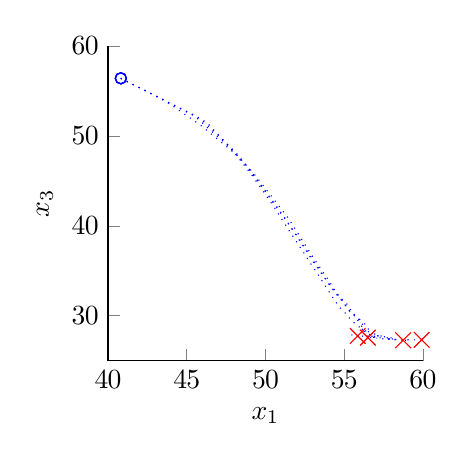
\begin{tikzpicture}

\begin{axis}[%
width=4cm,
height=4cm,
scale only axis,
xmin=40,
xmax=60,
xlabel={$x_1$},
ymin=25,
ymax=60,
ylabel={$x_3$},
axis x line*=bottom,
axis y line*=left
]
\addplot [
color=blue,
dotted,
forget plot
]
table[row sep=crcr]{
40.812346127662 56.390055551753\\
46.2544406630289 51.5146863585135\\
46.5786623595336 50.9161671122173\\
47.584863768256 49.0120535251562\\
48.205371440254 47.7375044795946\\
49.1597618958278 45.568707424969\\
50.5151014947123 42.1659638913025\\
51.041476465486 40.709199352669\\
51.4399559951573 39.6320847476969\\
52.3770953534623 37.1421179639705\\
53.041758466095 35.3342420564182\\
53.1800805465359 35.008435060617\\
54.3470782373836 31.8169641681409\\
54.709290938734 30.9370736578979\\
55.1312920047603 30.1709544485086\\
55.485023418837 29.4170037993968\\
56.007907681961 28.6766700578571\\
56.4239764808709 28.00394073261\\
56.7073807578253 27.899016139778\\
56.8308566744141 27.7777482528008\\
56.9659872119925 27.6463801031629\\
56.6301724350761 27.6827018009765\\
56.5540864419505 27.6983595044925\\
56.1236116262385 27.7536373276544\\
56.2355814915408 27.7039613171144\\
55.8439742330686 27.7793396714702\\
55.4549074376335 27.8721999574226\\
55.7010077547562 27.8027659032938\\
55.8563133460123 27.7559436106647\\
};
\addplot [
color=blue,
only marks,
mark=o,
mark options={solid},
forget plot
]
table[row sep=crcr]{
40.812346127662 56.390055551753\\
};
\addplot [
color=red,
mark size=4.0pt,
only marks,
mark=x,
mark options={solid},
forget plot
]
table[row sep=crcr]{
55.8563133460123 27.7559436106647\\
};
\addplot [
color=blue,
dotted,
forget plot
]
table[row sep=crcr]{
40.812346127662 56.390055551753\\
45.7061201093358 52.0859305486896\\
46.0610220107513 51.5512519238604\\
47.3783220162097 49.4485926422088\\
48.1674139704244 48.0266657334626\\
48.7795834436903 46.7460277933682\\
49.2783861352632 45.5625848402415\\
51.1650205382931 41.0329016814302\\
51.5583479983133 39.9789021296177\\
52.5764867817225 37.2489877308755\\
53.0360745494873 35.9752773299401\\
53.8348017089505 34.0130200812808\\
53.9442148565891 33.7137742893278\\
55.3333667512592 30.574869891379\\
55.5411547617714 30.2866439028251\\
56.1876685834383 29.144222922143\\
56.0377911490971 28.5668982712177\\
57.0879359142798 27.8656117034152\\
57.6591650678536 27.6191397223678\\
57.7352689829265 27.5376990119776\\
57.6734231261159 27.5227673692408\\
57.691157949152 27.4775287020364\\
57.6096115624066 27.4776979205826\\
58.0140912398712 27.4150913438817\\
58.4690260538382 27.3827966849873\\
59.003034776058 27.3536355226187\\
58.9675592596427 27.3443802332365\\
59.1771199201361 27.328140477336\\
59.3983238540247 27.3231358304048\\
59.9153382459389 27.3243136751789\\
};
\addplot [
color=blue,
only marks,
mark=o,
mark options={solid},
forget plot
]
table[row sep=crcr]{
40.812346127662 56.390055551753\\
};
\addplot [
color=red,
mark size=4.0pt,
only marks,
mark=x,
mark options={solid},
forget plot
]
table[row sep=crcr]{
59.9153382459389 27.3243136751789\\
};
\addplot [
color=blue,
dotted,
forget plot
]
table[row sep=crcr]{
40.812346127662 56.390055551753\\
43.4720645903032 54.0433059214293\\
44.4105331428893 52.9675244829451\\
45.1521362838879 52.0547328493258\\
45.917193834142 51.1182414098397\\
48.237030476867 47.78055664315\\
48.983232622263 46.348328144903\\
49.3006948723548 45.7026676596445\\
51.3506658811046 41.0788005533308\\
51.5174331589206 40.6537574795898\\
52.9280226375499 36.7534963088799\\
53.7316744841338 34.6263601093772\\
53.9627376379364 34.0877830432855\\
54.2769621786136 33.1407198127222\\
54.8206295930271 31.8021787359052\\
55.4603916551842 30.2129287437599\\
55.9061948301809 29.7125515229604\\
56.5060532444462 28.7721598476547\\
56.5621081450101 28.0903955263143\\
57.2327663961215 27.7242927605076\\
56.8743049294303 27.7369219679431\\
57.0036070520092 27.6886569356698\\
56.4235783370951 27.7724046743125\\
56.8037536445014 27.6807599436682\\
57.3123354831149 27.5494449162624\\
56.9469483912208 27.5978911557567\\
56.7640397245829 27.5929118947553\\
57.0881251188248 27.5266569076905\\
56.5211187469439 27.6002072274092\\
56.3745383522368 27.6009645428071\\
56.4999366255617 27.5707943493448\\
};
\addplot [
color=blue,
only marks,
mark=o,
mark options={solid},
forget plot
]
table[row sep=crcr]{
40.812346127662 56.390055551753\\
};
\addplot [
color=red,
mark size=4.0pt,
only marks,
mark=x,
mark options={solid},
forget plot
]
table[row sep=crcr]{
56.4999366255617 27.5707943493448\\
};
\addplot [
color=blue,
dotted,
forget plot
]
table[row sep=crcr]{
40.812346127662 56.390055551753\\
45.339543084018 52.3801375951014\\
45.6259236706153 51.9863854540182\\
47.5523466649108 48.9825809933166\\
48.2534043026836 47.6698625449513\\
48.9206387780633 46.3116028919991\\
49.5726158362278 44.8057057957677\\
52.2983114324176 38.1473146838141\\
52.45395470498 37.704813209981\\
53.1665953743211 35.8049989141859\\
53.5295425437654 34.8573149558381\\
54.3368754085646 32.759878103678\\
54.5853330001203 32.2324072513634\\
55.106720023102 31.4615931549509\\
55.7090931990632 29.8724553472055\\
56.029280678242 29.070888091489\\
56.2321589926358 28.4293166791616\\
56.7375245980328 27.9734397947316\\
57.0872072032991 27.7692238340827\\
57.7303094884906 27.6318096140969\\
57.9793767127412 27.5514544194754\\
58.1872844969287 27.4969409166947\\
58.0259288145659 27.4265257347795\\
58.1787054829581 27.415737597942\\
58.0144454802376 27.4270882771184\\
57.8810142964652 27.4000404211909\\
57.4142730645086 27.4544501047851\\
58.1262363044895 27.3475119667379\\
58.6445629716112 27.2979571110696\\
58.9811640743234 27.2730601776227\\
58.7371850412593 27.2756190698718\\
};
\addplot [
color=blue,
only marks,
mark=o,
mark options={solid},
forget plot
]
table[row sep=crcr]{
40.812346127662 56.390055551753\\
};
\addplot [
color=red,
mark size=4.0pt,
only marks,
mark=x,
mark options={solid},
forget plot
]
table[row sep=crcr]{
58.7371850412593 27.2756190698718\\
};
\end{axis}
\end{tikzpicture}%
}
%\subfloat[]{% This file was created by matlab2tikz v0.4.4 running on MATLAB 7.13.
% Copyright (c) 2008--2013, Nico Schlömer <nico.schloemer@gmail.com>
% All rights reserved.
% 
% The latest updates can be retrieved from
%   http://www.mathworks.com/matlabcentral/fileexchange/22022-matlab2tikz
% where you can also make suggestions and rate matlab2tikz.
% 
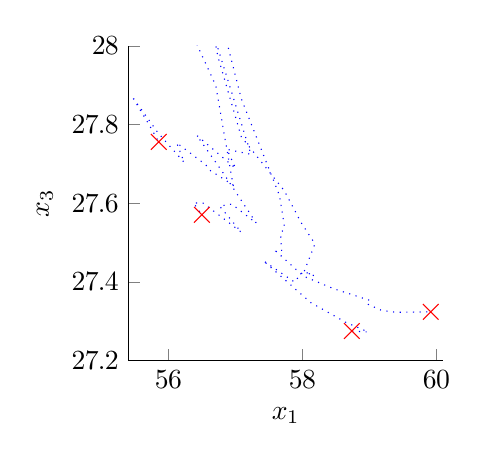
\begin{tikzpicture}

\begin{axis}[%
width=4cm,
height=4cm,
scale only axis,
xmin=55.4,
xmax=60.1,
xlabel={$x_1$},
ymin=27.2,
ymax=28,
ylabel={$x_3$},
axis x line*=bottom,
axis y line*=left
]
\addplot [
color=blue,
dotted,
forget plot
]
table[row sep=crcr]{
56.4239764808709 28.00394073261\\
56.7073807578253 27.899016139778\\
56.8308566744141 27.7777482528008\\
56.9659872119925 27.6463801031629\\
56.6301724350761 27.6827018009765\\
56.5540864419505 27.6983595044925\\
56.1236116262385 27.7536373276544\\
56.2355814915408 27.7039613171144\\
55.8439742330686 27.7793396714702\\
55.4549074376335 27.8721999574226\\
55.7010077547562 27.8027659032938\\
55.8563133460123 27.7559436106647\\
};
\addplot [
color=red,
mark size=4.0pt,
only marks,
mark=x,
mark options={solid},
forget plot
]
table[row sep=crcr]{
55.8563133460123 27.7559436106647\\
};
\addplot [
color=blue,
dotted,
forget plot
]
table[row sep=crcr]{
56.0377911490971 28.5668982712177\\
57.0879359142798 27.8656117034152\\
57.6591650678536 27.6191397223678\\
57.7352689829265 27.5376990119776\\
57.6734231261159 27.5227673692408\\
57.691157949152 27.4775287020364\\
57.6096115624066 27.4776979205826\\
58.0140912398712 27.4150913438817\\
58.4690260538382 27.3827966849873\\
59.003034776058 27.3536355226187\\
58.9675592596427 27.3443802332365\\
59.1771199201361 27.328140477336\\
59.3983238540247 27.3231358304048\\
59.9153382459389 27.3243136751789\\
};
\addplot [
color=red,
mark size=4.0pt,
only marks,
mark=x,
mark options={solid},
forget plot
]
table[row sep=crcr]{
59.9153382459389 27.3243136751789\\
};
\addplot [
color=blue,
dotted,
forget plot
]
table[row sep=crcr]{
56.5621081450101 28.0903955263143\\
57.2327663961215 27.7242927605076\\
56.8743049294303 27.7369219679431\\
57.0036070520092 27.6886569356698\\
56.4235783370951 27.7724046743125\\
56.8037536445014 27.6807599436682\\
57.3123354831149 27.5494449162624\\
56.9469483912208 27.5978911557567\\
56.7640397245829 27.5929118947553\\
57.0881251188248 27.5266569076905\\
56.5211187469439 27.6002072274092\\
56.3745383522368 27.6009645428071\\
56.4999366255617 27.5707943493448\\
};
\addplot [
color=red,
mark size=4.0pt,
only marks,
mark=x,
mark options={solid},
forget plot
]
table[row sep=crcr]{
56.4999366255617 27.5707943493448\\
};
\addplot [
color=blue,
dotted,
forget plot
]
table[row sep=crcr]{
56.2321589926358 28.4293166791616\\
56.7375245980328 27.9734397947316\\
57.0872072032991 27.7692238340827\\
57.7303094884906 27.6318096140969\\
57.9793767127412 27.5514544194754\\
58.1872844969287 27.4969409166947\\
58.0259288145659 27.4265257347795\\
58.1787054829581 27.415737597942\\
58.0144454802376 27.4270882771184\\
57.8810142964652 27.4000404211909\\
57.4142730645086 27.4544501047851\\
58.1262363044895 27.3475119667379\\
58.6445629716112 27.2979571110696\\
58.9811640743234 27.2730601776227\\
58.7371850412593 27.2756190698718\\
};
\addplot [
color=red,
mark size=4.0pt,
only marks,
mark=x,
mark options={solid},
forget plot
]
table[row sep=crcr]{
58.7371850412593 27.2756190698718\\
};
\end{axis}
\end{tikzpicture}%
}
%\caption{Four particle trajectories simulated from the same starting point using $\lgexpsf=0.3$, as used in the resample-move proposal stage. The second panel shows a close-up of the final states. This example uses the terrain tracking model from section~\ref{sec:numsim:tracking}, showing one horizontal and the vertical state component. Prior states are shown with circles and posterior states with crosses.}
%\label{fig:drone_rm_example}
%\end{figure}



\subsection{Step Size Adaptation}

An important practical consideration for implementing Gaussian flow sampling is how the sizes of the pseudo-time steps are chosen. State updates are calculated using local Gaussian approximations of the sequence density, with a best-case achieved with infinitesimally small steps between these approximations. In practice, the number of steps needs to be kept fairly low, to minimise the computational burden. In some instances, it may be sufficient to use a fixed step size, or a predetermined time grid chosen with a tuning run. However, an adaptive scheme is preferable for greatest efficiency.

Step size adaptation may legitimately be carried out separately for each particle. It is straightforward to see from \eqref{eq:state_update}, \eqref{eq:deterministic_weight_update} and \eqref{eq:stochastic_weight_update} that two consecutive updates using the same fixed values for $\lgmomapprox{\pt}$ and $\obapprox{\pt}$ are equivalent to a single update spanning both intervals. Thus, a large interval between update steps is equivalent to a number of shorter intervals with hypothetical intermediate update times aligned with those of the other particles.

For adaptive step size control, a measure is required which estimates the local ``error'' introduced by using finite rather than infinitesimal step sizes. We consider the state update for the interval $[\pt_0,\pt_1]$, and distinguish between the ``ideal'' dynamics $\{\flowdriftapprox{\pt|\pt},\flowdiffuseapprox{\pt|\pt}\}$ which use a continuously updated approximation, and the actual dynamics $\{\flowdriftapprox{\pt|\pt_0},\flowdiffuseapprox{\pt|\pt_0}\}$ which use the approximation formed at $\pt_0$. Integrating the different between the two resulting SDEs, we find that the error introduced by using finite step sizes is,
%
\begin{IEEEeqnarray}{rCl}
 \lserror{\pt_1}{\pt_0} & = & \int_{\pt_0}^{\pt_1} \left[ \flowdriftapprox{l|\pt_0}(\ls{l}) - \flowdriftapprox{l|l}(\ls{l}) \right] dl + \int_{\pt_0}^{\pt_1} \left[ \flowdiffuseapprox{l|\pt_0} - \flowdiffuseapprox{l|l} \right] d\flowbm{l} \nonumber      .
\end{IEEEeqnarray}
%
The integrands are both equal to $0$ at $\pt_0$. Hence, approximating each over the interval by half its final value, we arrive at the following rough estimate for the error introduced by the update,
%
\begin{IEEEeqnarray}{rCl}
 \widehat{\lserror{\pt_1}{\pt_0}} & = & \half \left( \flowdriftapprox{\pt_1|\pt_0}(\ls{\pt_1}) - \flowdriftapprox{\pt_1|\pt_1}(\ls{\pt_1}) \right) (\pt_1-\pt_0) + \half \left( \flowdiffuseapprox{\pt_1|\pt_0} - \flowdiffuseapprox{\pt_1|\pt_1} \right) \int_{\pt_0}^{\pt_1} d\flowbm{l} \nonumber \\
 & \approx & \half (\pt_1-\pt_0) \left( \flowdriftapprox{\pt_1|\pt_0}(\ls{\pt_1}) - \flowdriftapprox{\pt_1|\pt_1}(\ls{\pt_1}) \right) + \half (\pt_1-\pt_0)^{\half} \left( \flowdiffuseapprox{\pt_1|\pt_0} - \flowdiffuseapprox{\pt_1|\pt_1} \right) \snchange{\pt_0,\pt_1} \nonumber       .
\end{IEEEeqnarray}
%
The last line follows from the definition of $\snchange{\pt_0,\pt_1}$ using approximations for small $(\pt_1-\pt_0)$,
%
\begin{IEEEeqnarray}{rCl}
 \snchange{\pt_0,\pt_1} & = & \frac{ \int_{\pt_0}^{\pt_1} \dsf^{\half}\exp\left\{ -\half \dsf (\pt_1-\pt_0) \right\} d\flowbm{\pt} }{ 1-\exp\left\{-\dsf(\pt_1-\pt_0)\right\} }  \approx  \frac{ \dsf^{\half} \int_{\pt_0}^{\pt_1}d\flowbm{\pt} }{ \left[\dsf(\pt_1-\pt_0)\right]^{\half} } \nonumber \\
 \int_{\pt_0}^{\pt_1}d\flowbm{\pt} & \approx & (\pt_1-\pt_0)^{\half} \snchange{\pt_0,\pt_1} \nonumber      .
\end{IEEEeqnarray}

This formula also indicates that for small steps, the stochastic term is likely to dominate, and thus that the discretisation error is minimised by setting $\dsf=0$.

Pseudo-time step sizes may now be adjusted so that the magnitude of the local error estimate is kept below a threshold. For this purpose, step size control mechanisms may be borrowed directly from well-established numerical integration algorithms for solving differential equations (see for example \citep{Shampine1997}).



\section{Applications in Particle Filtering} \label{sec:gaussian_flows_for_particle_filters}

Our motivating purpose for studying particle flows is for use in filtering. We consider a standard discrete-time Markovian state space model in which the transition, observation and prior models have closed-form densities,
%
\begin{IEEEeqnarray}{rClCrClCrCl}
 \ls{\ti} & \sim & \transden(\ls{\ti} | \ls{\ti-1}) & \qquad & \ob{\ti} & \sim & \obsden(\ob{\ti} | \ls{\ti}) & \qquad & \ls{1} & \sim & \priorden(\ls{1})                  \nonumber      ,
\end{IEEEeqnarray}
%
where the random variable $\ls{\ti}$ is the hidden state of a system at time $\ti$, and $\ob{\ti}$ is an incomplete, noisy observation.

A conventional particle filter \citep{Cappe2007,Doucet2009} uses importance sampling to estimate distributions recursively over the path of the state variables, $\ls{1:\ti}=\{\ls{1}, \dots, \ls{\ti}\}$, such that,
%
\begin{IEEEeqnarray}{rCl}
 \sum_{i=1}^{\numpart} \npw{\ti}\pss{i} \phi(\ls{1:\ti}\pss{i}) & \rightasconverge & \int \postden(\ls{1:\ti}) \phi(\ls{1:\ti}) d\ls{1:\ti}      \nonumber       .
\end{IEEEeqnarray}
%
Each step begins by selecting a set of ancestors $\{\anc{\ti}{i}\}$ from amongst the ($\ti-1$)th step particles according to the corresponding weights. Next, a new state is proposed for each particle from an importance density $\ls{\ti}\pss{i} \sim \impden(\ls{\ti} | \ls{\ti-1}\pss{\anc{\ti}{i}}, \ob{\ti})$, and this is concatenated to the ancestral path to form the new particle $\ls{1:\ti}\pss{i} \leftarrow \left\{ \ls{1:\ti-1}\pss{\anc{\ti}{i}},  \ls{\ti}\pss{i} \right\}$. An importance weight is then assigned to the particle to account for the discrepancy between importance and target distributions,
%
\begin{IEEEeqnarray}{rClCl}
 \pw{\ti}\pss{i} & = & \frac{ \den(\ls{1:\ti}\pss{i} | \ob{1:\ti}) }{ \den(\ls{1:\ti-1}\pss{\anc{\ti}{i}} | \ob{1:\ti-1}) \impden(\ls{\ti}\pss{i} | \ls{\ti-1}\pss{\anc{\ti}{i}}, \ob{\ti}) } & \propto & \frac{ \transden(\ls{\ti}\pss{i} | \ls{\ti-1}\pss{\anc{\ti}{i}}) \obsden(\ob{\ti}|\ls{\ti}\pss{i}) }{ \impden(\ls{\ti}\pss{i} | \ls{\ti-1}\pss{\anc{\ti}{i}}, \ob{\ti}) } \label{eq:particle_filter_weight}     .
\end{IEEEeqnarray}

It was shown by \cite{Doucet2000a} that the weight variance is minimised by proposing from the conditional posterior $\impden(\ls{\ti} | \ls{\ti-1}\pss{\anc{\ti}{i}}, \ob{\ti}) = \den(\ls{\ti} | \ls{\ti-1}\pss{\anc{\ti}{i}}, \ob{\ti})$, known as the optimal importance density. This cannot be used routinely due to an intractable normalising constant required in the weight caluclations.



\subsection{Existing Particle Flow Approaches}

The approach taken by \cite{Daum2008,Daum2011d,Daum2013,Reich2011,Reich2012a} is to apply particle flow sampling directly to the filtering density. Assume that a set of unweighted particles exists approximating $\den(\ls{\ti-1}|\ob{1:\ti-1})$. The predictive density at the next step is related by,
%
\begin{IEEEeqnarray}{rCl}
 \den(\ls{\ti}|\ob{1:\ti-1}) & = & \int \den(\ls{\ti}|\ls{\ti-1}) \transden(\ls{\ti-1}|\ob{1:\ti-1}) d\ls{\ti-1}     ,
\end{IEEEeqnarray}
%
which can thus be sampled by simply drawing $\ls{\ti}\pss{i} \sim \transden(\ls{\ti}|\ls{\ti-1}\pss{i})$ for each particle and then marginalising (i.e. discarding) the old states. Defining this predictive density as the prior and the filtering density as the posterior, a particle flow is used to sample from,
%
\begin{IEEEeqnarray}{rCl}
 \den(\ls{\ti}|\ob{1:\ti}) & = & \frac{\den(\ls{\ti}|\ob{1:\ti-1}) \obsden(\ob{\ti}|\ls{\ti})}{\nconst{\ti}}      .
\end{IEEEeqnarray}
%
The difficulty with this approach is that finding an appropriate flow generally requires at least the prior and often also its gradient and Hessian to be calculable pointwise. This is not the case for the predictive density, $\den(\ls{\ti}|\ob{1:\ti-1})$. (Note that we could use a Monte Carlo approximation of this density, but the resulting algorithm has a complexity of $\bigo{\numpart^2}$ in the number of particles.) \cite{Reich2011,Reich2012a} address this by making analytical approximations of this density as a Gaussian or Gaussian mixture. \cite{Daum2008,Daum2011d,Daum2013,Daum2009c} use a number of methods, including Gaussian and various numerical approximations. These approximations alter the actual distribution of the particles. The filter is no longer exact, in the sense of returning a correctly weighted set of particles representing the posterior and providing asymptotically consistent estimates of posterior expectations.

Furthermore, the existing particle flow algorithms do not fall within the framework of ordinary particle filters. They only provide us with an estimate of the marginal filtering density $\den(\ls{\ti}|\ob{1:\ti})$, rather than the more conventional path filtering density $\den(\ls{1:\ti}|\ob{1:\ti})$. This may sometimes be all that is needed, but on other occasions samples of the entire path are essential, for example for smoothing or parameter estimation schemes \cite{Kitagawa1996,Andrieu2010}.



\subsection{Gaussian Flow Approximations to the Optimal Importance Density}

In this work, we use particle flow sampling within the standard particle filtering framework, thus retaining samples of the entire path and avoiding the need for additional layers of approximation. This is achieved by applying the particle flow sampling to the optimal importance density (OID) instead of the filtering density directly, by setting the prior and likelihood equal to the transition and observation densities respectively,
%
\begin{IEEEeqnarray}{rCl}
 \postden(\ls{\ti}|\ls{\ti-1}\pss{\anc{\ti}{i}}) = \den(\ls{\ti}|\ls{\ti-1}\pss{\anc{\ti}{i}},\ob{\ti}) & = & \frac{ \transden(\ls{\ti}|\ls{\ti-1}\pss{\anc{\ti}{i}}) \obsden(\ob{\ti}|\ls{\ti}) }{ \nconst{}(\ls{\ti-1}\pss{\anc{\ti}{i}}) }     .
\end{IEEEeqnarray}
%
To obtain formulas for the particle filter weight updates, we follow identical lines to the process in section~\ref{sec:weight_updates}. The difference here is that although the state updates are derived by considering the geometric sequence of densities approaching the OID, the actual target for the importance sampling is the filtering density. With this simple change, the required weight formulas in the deterministic and stochastic cases repectively become,
%
\begin{IEEEeqnarray}{rCl}
 \pw{\pt_1} & \propto & \pw{\pt_0} \times \frac{ \obsden(\ob{\ti} | \ls{\pt_1})^{\pt_1} \transden(\ls{\pt_1} | \ls{\ti-1}) }{ \obsden(\ob{\ti} | \ls{\pt_0})^{\pt_0} \transden(\ls{\pt_0} | \ls{\ti-1}) } \times \sqrt{\frac{\determ{\lsvrapprox{\pt_1}}}{\determ{\lsvrapprox{\pt_0}}}} \nonumber \\
 \pw{\pt_1} & \propto & \pw{\pt_0} \times \frac{ \obsden(\ob{\ti} | \ls{\pt_1})^{\pt_1} \transden(\ls{\pt_1} | \ls{\ti-1}) }{ \obsden(\ob{\ti} | \ls{\pt_0})^{\pt_0} \transden(\ls{\pt_0} | \ls{\ti-1}) } \times \frac{ \normal{\ls{\pt_0}}{\lsmnapprox{\pt_0}}{\lsvrapprox{\pt_0}} }{ \normal{\ls{\pt_1}}{\lsmnapprox{\pt_1}}{\lsvrapprox{\pt_1}} } \nonumber       .
\end{IEEEeqnarray}

%
%
%
%In the deterministic case ($\dsf=0$), the importance density implied by using $K$ state updates with \eqref{eq:state_update} may be computed by applying the change of variables formula $K$ times. The required Jacobians are as in \eqref{eq:deterministic_weight_update}. In the stochastic case ($\dsf>0$), we apply the importance sampling to the extended distribution over the product space for all the intermediate states $\ls{\ti,0},\ls{\ti,1},\dots,\ls{\ti,K}=\ls{\ti}$ using artificial conditional densities as in \eqref{eq:stochastic_weight_update}.
%
%
%
%
%%%
%%\begin{IEEEeqnarray}{rCl}
%% \impden(\ls{\ti} | \ls{\ti-1}\pss{\anc{\ti}{i}}, \ob{\ti}) & = & \transden(\ls{\ti,0}|\ls{\ti-1}\pss{\anc{\ti}{i}}) \prod_{k=1}^{K} \sqrt{\frac{\determ{\lsvrapprox{\pt_k}}}{\determ{\lsvrapprox{\pt_{k-1}}}}}^{-1}     ,
%%\end{IEEEeqnarray}
%%
%%where $\ls{\ti,0}$ is the initial state sampled from the prior.
%
%
%
%
%
%
%
%%
%Note, in this section we omit for clarity subscript $\ti$ on variables which vary with $\pt$, e.g. $\ls{\pt}=\ls{\ti,\pt}$.
%
%It is straightforward to conduct state updates using \eqref{eq:state_update}. Furthermore, if the true final density of the particle generated using the flow is $\impden(\ls{\ti}|\ls{\ti-1}\pss{\anc{\ti}{i}})$, then from the weight formulas in section~\ref{sec:weight_updates} it can be seen that,
%%
%\begin{IEEEeqnarray}{rCl}
% \frac{ \postden(\ls{\ti}|\ls{\ti-1}\pss{\anc{\ti}{i}}) }{ \impden(\ls{\ti}|\ls{\ti-1}\pss{\anc{\ti}{i}}) } & \propto & \frac{ \transden(\ls{\ti}|\ls{\ti-1}\pss{\anc{\ti}{i}}) \obsden(\ob{\ti}|\ls{1}) }{ \transden(\ls{\ti,0}|\ls{\ti-1}\pss{\anc{\ti}{i}}) \nconst{}(\ls{\ti-1}\pss{\anc{\ti}{i}}) } \times \prod_{k=1}^{K} \Delta_k \nonumber      ,
%\end{IEEEeqnarray}
%%
%where $\ls{\ti,0}$ is the state sampled from the prior at which the particle flow begins and $\Delta_k$ is the Jacobian or ratio of Gaussians from either \eqref{eq:deterministic_weight_update} or \eqref{eq:stochastic_weight_update}, depending on the value of $\dsf$. The particle filter weight formula \eqref{eq:particle_filter_weight} now becomes,
%%
%\begin{IEEEeqnarray}{rClCl}
% \pw{\ti}\pss{i} & = & \propto & \frac{ \transden(\ls{\ti}\pss{i} | \ls{\ti-1}\pss{\anc{\ti}{i}}) \obsden(\ob{\ti}|\ls{\ti}\pss{i}) }{ \impden(\ls{\ti}\pss{i} | \ls{\ti-1}\pss{\anc{\ti}{i}}, \ob{\ti}) } \nonumber \\
% & = & \frac{ \transden(\ls{\ti}\pss{i} | \ls{\ti-1}\pss{\anc{\ti}{i}}) \obsden(\ob{\ti}|\ls{\ti}\pss{i}) }{ \impden(\ls{\ti}\pss{i} | \ls{\ti-1}\pss{\anc{\ti}{i}}, \ob{\ti}) } \nonumber \\
%\end{IEEEeqnarray}
%
%
%
%
%
%The standard weight update formulas may not be used here, since the unknown normalising constant is not common to all particles due to the dependence on $\ls{\ti-1}\pss{\anc{\ti}{i}}$. However, particle filter weights
%
%
%
% Applying the Gaussian flow sampling to the OID is straightforward, setting the prior to be the transition density and the likelihood the observation density,
%%
%\begin{IEEEeqnarray}{rCl}
% \postden(\ls{\ti}|\ls{\ti-1}\pss{\anc{\ti}{i}}) = \den(\ls{\ti}|\ls{\ti-1}\pss{\anc{\ti}{i}},\ob{\ti}) & = & \frac{ \transden(\ls{\ti}|\ls{\ti-1}\pss{\anc{\ti}{i}}) \obsden(\ob{\ti}|\ls{\ti}) }{ \nconst{\ti}(\ls{\ti-1}\pss{i}) }     .
%\end{IEEEeqnarray}
%%
%The only modification required to the standard process is in the weight formulas. Although the particle flow is calculated based on the OID sequence, the target density for the importance sampler is now replaced by the filtering density.



\subsection{Simulations} \label{sec:simulations}

Numerical testing using simulated data is presented to demonstrate the efficacy of Gaussian flow sampling for particle filtering. Our primary indicator of performance is the average effective sample size (ESS), measured before resampling. The effective sample size at time step $\ti$ is defined as,
%
\begin{IEEEeqnarray}{rCl}
 \ess{\ti} & = & \left[\sum_i \npw{\ti}\pss{i}{}^2\right]^{-1} \nonumber      ,
\end{IEEEeqnarray}
%
which intuitively is an estimate of the size of an equivalent set of independent, unweighted samples. RMSE values using the empirical particle mean as a point estimate are also included.
%Comparisons are conducted by adjusting the number of filter particles such that the running times for the various algorithms are roughly equal.% However, they should be treated with caution, since when a distribution is irregular the particle mean may be distant from the true value even if the particles are drawn from it perfectly (see figure~\ref{fig:rmse_fail} for an illustration of this effect).
%%
%\begin{figure}[bt]
%\centering
%% This file was created by matlab2tikz v0.4.4 running on MATLAB 7.13.
% Copyright (c) 2008--2013, Nico Schlömer <nico.schloemer@gmail.com>
% All rights reserved.
% 
% The latest updates can be retrieved from
%   http://www.mathworks.com/matlabcentral/fileexchange/22022-matlab2tikz
% where you can also make suggestions and rate matlab2tikz.
% 
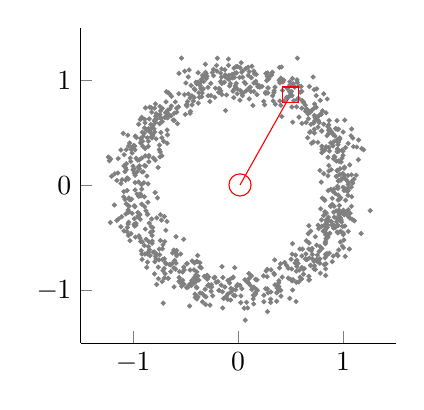
\begin{tikzpicture}

\begin{axis}[%
width=4cm,
height=4cm,
scale only axis,
xmin=-1.5,
xmax=1.5,
ymin=-1.5,
ymax=1.5,
axis x line*=bottom,
axis y line*=left
]
\addplot [
color=gray,
mark size=0.7pt,
only marks,
mark=*,
mark options={solid},
forget plot
]
table[row sep=crcr]{
-0.667808301803045 -0.881722985195889\\
0.590899554295771 -0.871328325686582\\
0.958596038215192 0.337384207762483\\
-1.04832161320494 -0.365213838426281\\
0.443333594122442 -0.731772812113626\\
-0.814004636210302 -0.433221065669795\\
-0.564753470337596 0.876856863184287\\
0.491263017995344 0.893964897963182\\
-0.138460958315242 -1.07413332009561\\
0.69129713964166 -0.432331601314232\\
-0.699803541604327 -0.532293928425655\\
0.24321867316349 0.803589630417398\\
-0.789395577197072 0.243347009529782\\
0.989892209657758 -0.257944904426644\\
0.941742872586263 0.62052035427489\\
0.661678246057421 0.456502543011598\\
0.766533571378546 -0.408809374267537\\
-0.988689613657882 -0.191052551571934\\
-0.693663214016822 -0.733218086361739\\
-1.08543637724215 0.295506491326525\\
0.393692853696168 1.12592390967471\\
0.64752943651953 0.730184325421229\\
-0.382765119440575 -0.86007759960592\\
0.388565056305001 -0.904855693804892\\
0.744393829263343 0.746145545255177\\
-0.0735662977363081 0.972799037175272\\
-0.598624998197096 0.797776362643584\\
0.669800688111655 0.637646594747823\\
0.559637766972498 -0.708923913029212\\
-0.689197267622258 0.651710330603379\\
-0.721964442747421 0.736672393291725\\
-0.149180110224196 -1.01055035361466\\
0.328972408551018 0.856676920070993\\
-0.340643283576427 -1.0278559918131\\
0.863263970340743 0.139826243251366\\
0.641189501558371 0.767015753020644\\
0.824605014237822 -0.13950640191135\\
0.907587468514002 -0.40366170335898\\
-0.777018661782544 -0.940831143213775\\
-0.0971145169517417 -0.902166800045331\\
-0.702610102032649 -0.696489991003141\\
1.02308700226669 0.362415998249972\\
-0.0682907316901517 -0.977571201311173\\
-0.568080442433596 0.750708047289807\\
0.958150071472328 -0.611781344330047\\
-0.4151728988544 -0.926292404550677\\
-1.21608000442502 0.251799825269372\\
-1.17851756550772 -0.183822169776365\\
-0.487439202640073 0.757834681378457\\
-0.893613986783137 -0.569320598538913\\
-0.915247913940711 -0.702371304483813\\
0.126090281073323 1.02884341750926\\
-0.0497476171443781 -0.988938159519704\\
0.510329714656992 -0.792988671480406\\
0.334322421864824 0.807168244460553\\
-0.490618066492956 -0.743932803643382\\
-0.782473428106782 -0.696972173873906\\
0.64282271030656 -0.698582367586337\\
0.746826259744716 -0.566863937497114\\
-0.0235595527646823 -0.990590585172215\\
-0.929625013993637 -0.08068556324222\\
0.350591720336093 0.938822682051724\\
-0.268065937301342 -1.13701288148378\\
-0.955220201438197 -0.254927599102349\\
-0.538391020618362 -0.958352426736507\\
0.348263493818591 -0.707001485236338\\
-0.548040261209711 -0.650665637333094\\
1.04915230256745 0.0324548408345385\\
0.968399405446224 0.445029454951694\\
0.904564918019631 -0.0564731709458418\\
0.264000595640847 1.0691373887525\\
-0.457281536548848 -0.803713006907125\\
0.744245110709481 0.637746146341279\\
-0.54729525581767 -0.905639899845972\\
-0.612107738449039 -0.783448393574179\\
-0.824159199163491 -0.317000532102442\\
0.724300442662036 0.914645935241019\\
-1.21760369659157 0.257407450991805\\
-0.528195845808482 -0.90080340264423\\
0.778998320017908 0.145576350432296\\
-0.978895864836441 -0.489719062346182\\
-0.234327645359237 1.04895240938562\\
0.0699810108884379 0.972906483501521\\
0.681617933137113 0.508863438093778\\
0.810276081518613 -0.432848909811788\\
-0.918659075824138 -0.175506624066766\\
-0.21590554822947 0.928289979752627\\
-0.918250212766879 -0.0330156105179478\\
0.677223574164136 -0.688925163766685\\
-0.878030503038427 -0.240123135862826\\
-0.678356178770489 -0.34001444541632\\
0.607992670259702 0.592868075518831\\
0.761628324288131 -0.376965147094999\\
0.905223535718338 -0.670483619174427\\
-0.871316668678074 0.532845833268455\\
-0.913157654550221 0.509469022696384\\
0.0956415655525585 1.12837069834016\\
0.0341120755656513 1.08206783275046\\
-0.797645729046851 -0.630908934762258\\
0.797804198065572 -0.598354232943918\\
0.26206851763029 0.890190643786905\\
0.77729106119149 -0.697500825002063\\
0.954951735826567 -0.251508523629621\\
-0.28089689516774 -0.868417295124391\\
-0.43765742670988 -0.717008498790515\\
-0.0390853922485055 1.12024944194871\\
0.285259303378234 -1.02052943877262\\
1.04733972953876 -0.0203599209830764\\
0.739018850130867 0.659145639824706\\
-0.863781604980753 0.456547697550744\\
0.83796248482363 0.693902791959038\\
-1.0235922443101 0.231441967557046\\
-0.439158975404782 0.770383081226911\\
0.997864657459364 0.328349154516237\\
-0.466400629524291 1.10311380636838\\
0.999092185360782 0.288900014649883\\
0.93588773363831 0.234633458085366\\
0.696018747765178 -0.618728683944582\\
1.07879352863004 -0.196519028295715\\
0.0293253362730896 1.17167508525459\\
-0.671166872501909 0.647235988403063\\
1.06333191002087 0.198751782727311\\
0.796349439285446 0.520445318698689\\
-0.518389423606682 -0.774686521691341\\
-0.0358341149806878 1.03098973502207\\
-0.220288207018355 -0.871968972477749\\
0.999664465837211 -0.0156047318893743\\
0.722714383954118 -0.722067258545664\\
-0.120221875237786 0.71595167010745\\
0.340270830904237 0.884849258305063\\
0.539179365130363 0.938941994206693\\
-0.810683115297033 0.574694029065141\\
-0.686760942018893 -0.745311283936813\\
0.0911501153155632 -1.1645786728477\\
-0.393677494207003 -0.971832268128318\\
0.782453590469696 0.812149899700526\\
-0.242589284114598 -1.04920366928304\\
0.502016757079957 0.871636097508861\\
0.461435323390605 -0.759636526080518\\
-0.587987051662087 -0.647673118067338\\
-1.10907022864893 -0.295907597570905\\
0.953890280702658 -0.0892483520836509\\
0.838809903922967 -0.453088712160819\\
-0.0289945251391166 -1.04851371337284\\
1.01016895257089 -0.0223132111726885\\
0.915269176014708 0.279130510072653\\
-0.759295065839388 -0.885534217856085\\
0.251871176681959 0.770975640043413\\
0.761104691979236 0.558270807470188\\
0.121470297607646 0.897211657971966\\
-0.462716863630027 -0.938797923657095\\
-1.15561563650411 -0.330678047985517\\
1.1300539624623 0.36857047782192\\
-0.397821877285227 -0.888361858762085\\
-0.513748577004172 -0.801973720891384\\
-0.931050696792189 0.630657216448031\\
-0.454372233157627 0.707906125661802\\
-0.347019555884468 0.913661233086887\\
-0.981279612648722 0.0993452206891494\\
0.149245341883064 -0.96674102206459\\
-0.585872795369574 -0.617800844982993\\
-0.740791567046348 -0.522159077080093\\
-1.09024673685954 -0.106635466695319\\
-0.457959531064519 0.835247541440581\\
0.93834350167608 0.0882997755553118\\
-0.493932431462164 0.769426235688248\\
-0.893385125035128 -0.105687768262198\\
0.867801571030679 0.545075756758782\\
0.835810645828014 -0.504447118793926\\
1.00434071622208 0.0755559646994897\\
-0.549772495662947 -0.925174098821907\\
1.14720767867896 0.435444612284702\\
-0.457292042569689 0.689554066277473\\
0.241683879246124 -0.859232825165314\\
0.068154428602556 -1.28091481876601\\
-1.22619510192533 0.237308087502076\\
-0.0810866529140574 -0.927191760627475\\
-0.350958053754694 0.99225742118614\\
0.557856187169052 -0.712341047795554\\
0.743899852903384 0.857533108171898\\
0.792519290026698 0.679251381606344\\
0.285138737474197 1.02402344125736\\
-1.01470628401088 -0.128339941748411\\
-1.01030610888483 0.310785722515346\\
-0.809635380887342 -0.634297834267933\\
0.974849862597714 -0.305289527918656\\
-1.11672241210644 0.339679074986197\\
-0.709323398391025 0.423487052718002\\
0.883705171780518 -0.195802095978324\\
-0.871153329566429 -0.778073954916359\\
-0.63615080796645 0.758957461930545\\
1.0133631268214 0.0994800348255148\\
0.856023789005256 0.269672460051015\\
1.17206803289129 -0.454959531774735\\
0.408396530778534 -1.05201118501463\\
0.477321261571208 -0.880746998346162\\
0.261643101480271 -0.980580976465825\\
-0.730014359901352 -0.328256694158822\\
-0.0708258319047318 -1.08904094713436\\
0.78576219590824 0.682813425513284\\
-0.722648940428026 0.60999793020358\\
0.622390788779564 -0.84190403481708\\
-1.06428175131023 0.209039078847725\\
0.141168910567114 0.764599435892062\\
-0.260457349883568 0.974627137661542\\
0.972941900109951 -0.333583814674012\\
0.149258635283595 1.09122375492612\\
-1.00097257070218 0.18682924916186\\
-0.781258700164249 0.446067947200502\\
0.665490857129605 0.68463232573167\\
0.901042454824296 0.491175807317333\\
0.796454097748812 0.523581909810064\\
1.04558094415005 0.0978333110457382\\
-0.246073947892283 1.07882012316775\\
0.815241538134704 0.875070556224685\\
-0.947204431484797 0.585150815651541\\
0.719589332495156 0.734865381710928\\
0.546500099762253 -0.661991618251229\\
1.05945941322451 -0.602729516286905\\
-0.974075356902683 -0.375953954702745\\
-1.23640847996389 0.273435751212793\\
-0.713244406676058 -1.1183015448874\\
-0.00858629591001393 0.876211212877177\\
-0.475031221578571 1.03695352740644\\
-0.409108078907775 -1.06374418584844\\
-0.165028501430439 0.903873146237453\\
-0.85058970015313 -0.533437582826029\\
-0.972677540217194 -0.358159291702819\\
-0.860206603140441 -0.271361365602393\\
0.277537454920851 1.04090978865226\\
0.104500170989086 -0.884251738238874\\
-0.903686575231285 0.133027199693972\\
-0.0692736332280648 -1.01225937564836\\
1.10430512711692 0.0629558399028275\\
0.921227916262035 0.473890245273084\\
0.277265751485402 -0.797262929427682\\
-0.855949297698202 0.37414229463542\\
-0.12219597381699 1.05540559689993\\
-0.641985229129278 -0.817947242535005\\
-0.726262023671201 0.457148245562088\\
-1.146105503549 0.121005236259638\\
0.672690141606942 -0.602751298485629\\
-0.941844205195533 0.162654821937826\\
-0.268851907324754 -0.960976335101861\\
-0.539328092050764 1.21553836920286\\
-0.777601879479771 -0.650017291801728\\
-0.853173420255501 -0.580337781853743\\
0.558570019219566 -0.770013250656554\\
-1.07242947941834 0.0518543006504472\\
-0.885511480528125 0.353418021200835\\
0.143007357355829 -1.07811768468527\\
-0.956090056017594 0.242578818848662\\
0.897177816711859 -0.120115649660592\\
0.341735997714063 -0.835496674900597\\
-0.384057074366866 -1.06028889777334\\
0.725816971144409 0.669172424333504\\
0.148229313444823 -1.12638058111333\\
-1.11647686132493 -0.391007327245977\\
-0.417698305828087 0.922229138604245\\
0.385689382338903 -0.926159111437324\\
0.312222123553459 -1.01226360734139\\
0.977756230625122 0.0524403208381612\\
-0.00404882627231571 -0.947265253504143\\
-0.123875776647557 1.04038257799781\\
-0.3863156841092 -0.664751960373416\\
-0.595003737191002 -0.627421536295606\\
-0.839482033337832 -0.665148959684157\\
0.523910964639301 -0.896429249424378\\
1.09224478436964 0.453877569156271\\
0.831966275082742 -0.653951607727316\\
-0.831841433198404 0.582576261560821\\
-0.0917748204069953 1.14629329885941\\
0.642622026160543 0.709968460422486\\
0.162904138697436 -1.02177622190802\\
-0.302379866656473 1.02145844181619\\
0.863729056963064 0.191921080637353\\
-0.234516670483334 1.10879624160753\\
-0.356565688739298 0.928841001607055\\
0.834484450056983 -0.468140381410713\\
-0.747682302717793 -0.658409668520141\\
0.0799904954508625 -1.11062923216295\\
-0.327512633563884 1.04033458635637\\
0.727667980643732 -0.764691732086854\\
-0.983367536889443 -0.201010126849121\\
0.0369086335486468 0.879355931253222\\
0.765034712798519 -0.714069573107452\\
-0.81351625407611 -0.397849337021749\\
0.833314510651131 -0.792259004931042\\
-0.875903036085837 -0.510201979532712\\
-0.991080878416594 0.381525307166928\\
-0.793816340126028 -0.724847218091819\\
-0.81293121708733 0.483732118089385\\
-1.04141726898604 -0.252237980818292\\
-0.166901456576583 0.992434133631093\\
-0.86540498182129 -0.274088147660149\\
-0.259454559431281 0.85884229868154\\
0.177024285614818 -0.988390190868577\\
-0.775141180270636 -0.307149166588456\\
-0.558769066435354 -0.817314716729453\\
0.969259580553034 0.230012288844705\\
0.827267214759068 -0.688039644661799\\
0.971515614404361 0.161915076471627\\
-0.931932915771929 -0.319773882401281\\
0.965114063219301 -0.188652933703429\\
-0.166754320430172 1.07254201943642\\
1.00355705646447 -0.591152135142351\\
0.722408207994746 -0.793161810836773\\
0.406379597256678 1.02385211518389\\
0.605579637607375 0.898810103100275\\
-0.794728854271528 0.512064120525439\\
-0.0866054641666525 1.05132051136746\\
0.673474506747295 -0.862747028884817\\
-0.297475822713326 1.04245996068129\\
-0.682899493290733 0.894912291426189\\
0.105126984831249 1.0861369110088\\
0.319258213103347 1.05435810185015\\
0.946003125554549 0.146847248015778\\
0.858498089316551 -0.330804575881072\\
0.803753184761128 0.713346613047979\\
0.4217809334449 0.907583070992543\\
-1.00512036619209 0.365838037509694\\
-0.20180501423167 1.09130363474162\\
0.689122970832581 -0.758923907117299\\
-0.561794631896287 -0.874656779043453\\
0.796077573851317 -0.386886847810685\\
0.280917594841354 1.07480127676123\\
-0.845742928287501 -0.356466450845489\\
-0.751500925434114 -0.604275545191401\\
-0.796668357144537 -0.84004811023377\\
-0.982180632349305 0.342008216301961\\
0.587661321628764 -0.603932208467939\\
-1.15427993646308 0.0495143435216125\\
0.962523798849993 0.332184473042231\\
-0.819015789039567 -0.548196476472224\\
-1.01858586331501 0.344641051617378\\
-0.856226951998335 0.523865621874906\\
1.00767782274998 -0.517582006406834\\
0.388860474112865 -0.962299055256202\\
0.995016295450581 -0.388692977533354\\
-0.857725382619865 0.0179958145183476\\
-0.853439149627511 0.544074261423581\\
0.887595272516047 0.153225067609135\\
-0.160893349434528 -0.946283992333263\\
-0.741056381318369 0.65243051351096\\
-0.110546052514475 0.864210465684665\\
0.11516697488606 0.939313011689848\\
-1.05126158375409 0.480705480332925\\
0.928730780229125 0.543374682035939\\
0.492546990576149 0.990773570731726\\
-1.04066450003491 -0.193912303402632\\
0.888811111175868 -0.34068272461196\\
1.04595704623248 -0.0921533501471436\\
-0.312191855255317 1.15720981503044\\
0.700034451216566 0.403533892483998\\
-0.527721385371394 -0.822387278811598\\
0.0646256562144981 -0.895691448237941\\
-0.784889950734651 0.659728972276664\\
-0.417044748432267 -0.876625691115871\\
-1.02985339535142 -0.523020792752693\\
-0.66423104236077 0.683547741674715\\
-0.34858984296067 1.01280790649616\\
0.770688591635924 -0.626874327054871\\
0.462757359898273 0.841493901312344\\
-0.111632081076089 -1.05139673606593\\
-0.854874122930247 0.423045348610127\\
-0.795978214440634 0.738270741652193\\
0.143906909329042 -1.04356153335467\\
0.883472178914973 0.516294124380339\\
-0.394107631105802 0.970471791199284\\
-1.0585055106597 -0.436832902705586\\
-0.721309872437655 -0.599925950129187\\
0.826337091284127 -0.247702727167765\\
0.729440475848548 0.61651668544803\\
-0.426577503769703 0.806549664354219\\
0.512362593873538 -0.906568493659473\\
1.19531530675432 0.341583147156673\\
0.842896966621484 -0.345977052903907\\
1.00199014286787 -0.233510520089754\\
0.285349040833541 0.930426989756283\\
0.856194705289449 -0.489531299433064\\
-1.04298212501691 -0.347779944490992\\
-1.03340476868191 0.406595988254509\\
-1.05457368985666 -0.398438475953346\\
0.467774947644944 0.840420547653271\\
1.00213226179247 -0.451354990881969\\
-0.380237018979932 0.786363929803229\\
0.675870016176007 -0.545432822243632\\
0.678356476094576 -0.894216541229665\\
-0.844307494560009 -0.609846189060385\\
-1.04413789000404 -0.244011964679226\\
-0.738678189894726 0.712774686065542\\
0.0866634240452966 -0.917643486136155\\
0.180123993820591 -0.897279735187694\\
-0.418882609416212 0.841005517060687\\
0.0578954552234797 -1.16695392179055\\
-0.916350038800798 -0.650383901403034\\
0.941153956411702 -0.312054743047539\\
-1.04489066772557 -0.47408000327335\\
-0.821168829466298 0.455411338747105\\
-0.868458220884821 0.0921571823985022\\
0.693191707454563 0.5843978431478\\
-0.538455686834876 -0.928473794584643\\
-0.814992489966432 0.472870865491635\\
0.762169825784596 0.659499801929888\\
-1.03656557128103 -0.131521280972175\\
-0.720798406866567 -0.704701218939676\\
1.09765666989585 0.372185485972441\\
0.998283966935917 0.116372184992737\\
0.950725074205456 -0.668005136637602\\
0.245187478303365 -1.10524703561824\\
-0.856363868867144 -0.633350389234198\\
-0.146752610315841 -1.16447232499084\\
1.02018312269411 -0.673446437559223\\
0.857615258581302 -0.0465393997950644\\
0.38981321318085 -0.990775830774481\\
-0.890063833775547 -0.199987977790189\\
-0.415668051318913 -0.734673760877826\\
-0.0925735666334891 1.20619452749919\\
1.0138215139705 0.17722857669584\\
0.902107233802749 0.496200064501841\\
0.833832353574942 -0.855308868402668\\
-1.06612095831405 -0.1731030967631\\
-0.0298890920140226 1.07236180547069\\
0.828705992542359 -0.544200634253939\\
-0.00631534189771661 1.13501825157025\\
-0.0861901499292768 1.01283249436782\\
0.663407633279618 0.721808681379882\\
0.149311183367071 0.897456032634264\\
0.46891585460862 0.926332406931556\\
0.516837484735147 1.02184735577867\\
0.647788696001679 0.602371944707029\\
0.154464096620103 -1.04708663450103\\
-0.837812258125643 0.53396955463457\\
-0.14573934722625 -0.874240894145505\\
0.0255962499862039 -1.11354668729686\\
-0.511403642575789 0.866710863394879\\
1.00917250400608 -0.0454401552673083\\
0.845936052711327 -0.647317454127555\\
0.977403437531152 -0.114551058678258\\
0.73554379828387 -0.485308277666455\\
-0.715589425276968 -0.562272829580073\\
0.311634144864764 1.05270010986014\\
0.952091302244014 0.328165203056756\\
-0.889833594691766 0.631637530865458\\
1.02461937441359 -0.138508715510663\\
-1.09505411194548 0.49850317757307\\
-0.363845290650588 -0.774186079767654\\
-0.988967475535129 -0.31461765116733\\
0.814748324529423 -0.283690690237331\\
-0.882982895931956 0.741538403694135\\
-0.373231562106608 0.97531685074593\\
0.91396846047338 -0.0314537767423119\\
0.778471552107567 -0.738868888876072\\
-0.797604478356101 0.615760103574057\\
-0.6091973566572 0.622393483575315\\
-0.401584469968052 0.985800313427769\\
0.630117836726968 -0.789906159423761\\
0.312903132249725 -0.801783315252392\\
0.519487966041516 0.605189037638191\\
0.835913196176747 0.359265549985363\\
-0.0989592767377069 -1.08221027807677\\
-0.048860074647943 0.900905144479517\\
0.973696414225488 -0.535638999464622\\
-0.834790051603457 -0.444056550876979\\
-1.10531640845961 0.0573281558516577\\
-0.126513761858197 -0.965250065815603\\
-0.205934923161438 1.14529168664764\\
-0.381103660183856 1.07576803379727\\
0.792261328880616 0.0339409098839133\\
0.884766275902011 0.519550621233597\\
-0.944109973256369 -0.478229567490445\\
0.85930221652125 -0.300636814681584\\
0.94434907303855 0.350033360919837\\
-0.385959522453648 -1.05689597662131\\
0.921112663333076 0.273995417459087\\
-1.1404333481177 -0.317968015161483\\
0.910780271987199 -0.375685253808776\\
0.042685531278905 1.09174969182997\\
0.414566577476706 0.660184587872756\\
0.911904518585278 0.418910260232654\\
-1.01008851290735 -0.263476922126889\\
0.821691505880389 -0.375774307317124\\
0.513005828322252 0.858059585404666\\
-0.311183309364421 1.07960447058684\\
-0.981396111605855 0.029473803161953\\
-0.252075850556008 -0.964042834458097\\
-0.888706145193119 -0.650545986681808\\
-0.296613355631556 -0.885425285975272\\
0.622064546928295 0.791140139902379\\
-1.02290567258622 -0.13317804922773\\
-1.04484012642809 0.0641421723255906\\
-0.928596118477098 0.407362417776384\\
-0.928790969827976 0.450668569770071\\
-0.747812998923971 0.590582634869318\\
0.954167741658233 -0.24634060233055\\
0.908439829694859 0.25670231346952\\
0.491575683756469 -1.07277823874765\\
1.08163156028874 -0.104527799897836\\
-0.938621169410389 -0.272029860111518\\
-0.294711941834595 -0.890053723466589\\
-0.90878620983279 0.423472123315937\\
-0.19740395326087 1.21358435945998\\
0.866664091793122 -0.460622645822622\\
0.292048052297944 1.0172877785525\\
0.951535890204199 -0.136539098892911\\
1.03411841677005 -0.0493616913047976\\
0.655805463681331 -0.703886206772594\\
-0.0771212815463974 -0.890531327680305\\
0.167590616490702 0.994592428099454\\
-0.818014871999921 -0.526907249078452\\
-0.913295267408166 -0.535938532992927\\
0.310046370780783 -1.11222042226624\\
0.981048142790246 0.226138756761482\\
0.793687282603105 -0.325092935258327\\
-0.741743927369665 0.321894364477068\\
0.271611761647721 1.00045650760349\\
-0.327423184524429 0.992372032684239\\
0.385595956901397 -0.998613825023112\\
-0.382222780894802 0.987743895908876\\
0.0240791125723688 0.90393405895514\\
-0.93685915722752 -0.277765563955692\\
-0.00657667242759534 -0.942314729359396\\
-0.81518637639949 0.555085213567959\\
0.668254136743957 -0.456287557775236\\
-0.610054455485738 -0.96392430767991\\
0.437407800695623 0.809620075862774\\
-0.898134433885151 0.0280260293494908\\
0.759572370109833 0.412705598548584\\
0.733225202920335 0.650558544703969\\
-0.255412128827324 -0.943789361611764\\
0.735269621108258 -0.798529541128531\\
0.514338160234197 -0.651900060825787\\
1.04826379862287 0.402709607606913\\
-0.849334199158229 0.287644651330627\\
0.754903930239918 -0.661362021988652\\
-0.625046723565695 -0.641178429896059\\
0.51230523454532 0.749472708283398\\
-0.498397682247892 0.97820670250067\\
0.649769177475309 -0.52400224250084\\
-0.154488424419722 0.86871770146907\\
0.551346212736344 -1.10324617555315\\
0.922506708284227 -0.400037458556104\\
-0.7902801505955 -0.065027739510381\\
-1.02045078310106 -0.456108613648825\\
-0.374690212727787 0.884681673963178\\
0.718618381090638 0.596605500968238\\
-0.940141946511833 -0.0820069047939189\\
0.869297369516177 0.329812892972745\\
-0.703253512786528 -0.879299137718459\\
-0.980555420696217 0.472486209507172\\
0.763645854458336 0.621395645151432\\
-0.340046022020155 1.05091996677793\\
-0.992157079225235 0.162944797488928\\
-0.285915221627316 0.857561044647562\\
-0.824300060920593 0.741361761820721\\
0.645909310239443 -0.64995830513077\\
0.95042326248975 -0.0263155187175271\\
-0.648814689111751 0.731816620903565\\
-0.489529935548167 -0.970961144545729\\
0.0442987759732098 0.880905908889192\\
-0.676357259050719 0.404837092540585\\
0.95095376786446 0.39080225289186\\
0.706679318870003 -0.655020656854684\\
1.07772110258415 -0.0142215334949019\\
-0.411252666946557 -1.03312791428441\\
-0.586493850317636 -0.66702014382071\\
0.0349072352192829 -0.98165442006197\\
1.06671461407158 -0.263168308505922\\
0.800933564999022 0.345088248716668\\
0.726447105721767 0.50138216563235\\
0.15564744130307 1.06452699633931\\
0.562805893702201 0.984041486508919\\
0.501681828392411 -0.893803630023711\\
-0.564504229020649 -0.911142852085469\\
0.944492325760261 -0.379191004624931\\
-0.043416343702455 -1.04287256148333\\
0.620673899286045 0.800795472136453\\
-0.591837109232279 -0.48534259015009\\
-1.08882268465372 -0.0557531149260014\\
0.390275797953387 1.00406396699049\\
-1.04344340575745 0.378048616001528\\
-1.07354878306597 0.172403585016962\\
0.517487178303015 -0.901913492290251\\
-0.222008047751969 0.84187806647481\\
-0.744718160679364 0.274002624859978\\
0.180447854084113 0.867421848992235\\
1.00156373691985 -0.466691882388449\\
0.863535986042712 0.578932391498324\\
0.0164835848248436 -0.948563918517236\\
-1.04765397167023 -0.231911377380672\\
0.815467454443038 0.114512636622841\\
0.903573463769454 0.379668207848408\\
0.847181953876968 0.476380742042593\\
-0.627664204925295 -0.741290234739159\\
0.80167742596025 -0.118118746709467\\
-0.953758148024417 -0.296313660389423\\
0.987238411103203 0.0664806811497406\\
0.853625890281761 0.563872654769654\\
-0.734326323659055 0.6375630452259\\
-0.0151014285941866 1.07459874610113\\
-0.745142329534568 0.678004270793314\\
0.283623197343571 0.883399218665226\\
-0.130831760331835 0.985105111351197\\
-1.08781991389039 -0.430441634576366\\
0.406004730739487 -0.996999418303859\\
-0.918605821537921 0.651249913028848\\
-0.339487915489357 -1.1061559063411\\
0.967919925336474 0.456675139963644\\
1.04902376558669 -0.435503549860458\\
-1.0572125405428 0.0745232732507498\\
-0.725387314024043 0.285465638905061\\
-0.73619363361394 0.506832599803121\\
0.0269131386571799 -1.05018893555178\\
0.115822327578791 -0.948331935836743\\
0.171791652165361 1.06030549691216\\
-0.361807653876019 -1.02156233655826\\
-0.787015145840792 0.603532767949549\\
0.0417589993760137 0.858687245172198\\
1.01536978221839 0.623974737570518\\
0.820595805990183 -0.751590191445807\\
0.491381873768873 0.8527703702619\\
0.99373602621712 -0.576517069851963\\
-0.827821522798391 0.497436582859439\\
-0.841836688748777 0.517229996216529\\
-0.363881627596579 -0.733719466988662\\
-0.58458399549003 0.699942165861055\\
-0.186290112390162 0.889230988812051\\
0.642245164111045 -0.697326274577691\\
0.606971069023936 -0.669298305708626\\
-0.884143787228878 0.284192133701564\\
-0.0418225250787287 0.83864121900889\\
0.261871728650717 0.87743932048112\\
-0.638139485039273 0.665434816477899\\
-0.762457554684469 0.173547187922538\\
-1.06446924971222 0.153048114855554\\
0.851659742311547 -0.372282500446442\\
-1.00116138618316 0.150727863554446\\
0.0421481943267013 1.03288747196555\\
0.613129603576911 -0.604352120047525\\
0.420573901542569 -0.871300211213377\\
1.00936620119158 0.165866888361166\\
-0.842268649939163 0.748402427128168\\
-0.613527790050471 -0.612456545237488\\
0.27895742300414 -0.983500594233258\\
-0.777985862076247 0.669860730455579\\
0.600198301450173 0.945108271839314\\
-0.397351756209121 -0.966929274417568\\
0.956911667925961 0.235481184271275\\
0.245868442288346 -1.04328366294975\\
-0.963685681867639 0.132028809298227\\
0.955025868492955 0.418504499612164\\
-0.676338101863419 0.529887732426076\\
0.606677879505853 0.738479615206158\\
0.72809732942978 0.778105189124852\\
0.325553433549419 1.08054807304777\\
-0.102810237972662 1.02201003965492\\
-0.800742028534436 0.541356995024618\\
-0.403626513967661 -0.913648099310745\\
0.373138756928856 -0.975799171024959\\
0.553540864229142 -0.814672153151568\\
-0.0968934593945304 -1.03156573912524\\
0.830225812984339 -0.420905754933129\\
-0.332520467885951 0.922268405268296\\
0.95590623963149 0.0469267511714368\\
1.00023683805018 0.510802324142237\\
0.434537773936088 1.0052884787775\\
0.916312532384142 -0.29937171108109\\
0.128074201374134 -0.858281692463807\\
0.0963108305977138 1.05054598106682\\
-0.34318476456303 0.882707652538296\\
-0.941068813986284 0.245527025509685\\
0.931501569800703 0.542770320897772\\
-0.440858114548491 -0.903120483399613\\
0.350581898182525 -0.944067422186858\\
-1.04095109807482 -0.115995198670214\\
-0.787915556380085 0.778797505489057\\
-0.695117153939915 -0.838523302385129\\
0.131296488001624 -0.988558668157714\\
1.07559011263963 0.475507732476055\\
0.397159226733026 0.807286916827855\\
-0.91765944638639 0.262943837770768\\
1.04976358491089 -0.0465171446283656\\
-0.75395782654025 -0.70610272939003\\
-0.00799313475706689 0.923156535056275\\
0.914190910650423 -0.195116075180997\\
-0.359047687457581 0.952004972032713\\
0.97488865495983 -0.317414584290176\\
0.101903626780376 -0.836420913859782\\
-0.295939115771586 -0.852956917451026\\
0.956966142925994 0.53913771836222\\
-0.891533536072478 0.191007637751001\\
0.945412023178621 0.53610272608365\\
-0.935241137239362 -0.499575751022441\\
0.842365389536629 -0.665898353572366\\
-0.98976152530997 0.118683287934272\\
1.08842513455301 -0.321936152322016\\
0.393931837175672 -0.7822267966597\\
0.563481156679386 0.820486556028572\\
0.94215168442349 -0.440945100345125\\
1.01777650998491 -0.384175388777636\\
-0.984002505260258 0.377335302047564\\
0.797922607672177 0.314208407496376\\
-0.64351556377593 -0.753891408077623\\
0.94554555965851 0.142046625004416\\
0.716956051928088 0.416782851480425\\
0.27674867154477 -0.866390385601947\\
0.576809048394681 -0.916618307480877\\
0.0745708942207465 0.901481716874972\\
-0.183451914621485 -0.997232943500438\\
-1.21731692098608 -0.350671163196632\\
-0.604972500164042 -0.711640497718426\\
0.82224075738174 -0.131141310156057\\
0.397095573943563 0.980713772533441\\
-0.739711865590086 -0.276337804376406\\
1.02837674215579 -0.25627159400144\\
-0.306103620664092 -1.05849315991596\\
0.883431017460554 -0.0325499016417889\\
0.797209394009298 0.376261899187362\\
-0.705206414883056 -0.788675046352264\\
0.608153734439333 -0.778909994701527\\
1.08746430830482 0.0476523452358789\\
0.706825954221285 -0.695680740024363\\
-0.751470547812262 0.344120050748824\\
0.855509851916964 0.0940930433101727\\
0.689220699347366 0.70175765800414\\
0.958654857244502 -0.231036564564353\\
0.829516975130694 -0.418404120398416\\
-1.11630835978165 0.0217428567687688\\
0.366780524817447 -1.10006883838103\\
0.77997940834441 -0.579065645162954\\
-0.483285659453372 -0.742150013322891\\
0.838177474429287 -0.325829671197118\\
-0.596430443685918 -0.794935358046434\\
0.896451951824164 -0.723275702828362\\
-0.447807946758168 0.95361635567306\\
0.0731494958168391 1.11560252631557\\
0.406502240273527 0.765889305854214\\
0.955541524038158 0.337511112743921\\
0.582945271057743 -0.804470508377598\\
1.04684223089101 -0.291290915788936\\
0.426144387401504 0.988477592825288\\
-1.06508940531597 0.343020248780181\\
-0.947903861985563 0.0350031176910546\\
0.747945602033921 0.922838625467046\\
0.507053299113194 0.897495697830812\\
-0.154689748153642 0.973406361411993\\
1.10663792083398 -0.333691956273461\\
0.0991657797086641 -0.92616464840736\\
-0.863192512904915 -0.728327858510874\\
-0.228497642269932 -0.878140158905908\\
1.04846609214639 -0.229556613484958\\
1.0294818760524 0.0566931569160079\\
-0.347542257714384 0.848136032446601\\
-0.673576742685214 0.484185061863253\\
0.951785158158741 0.41361804649842\\
0.679155371881611 0.944685663415331\\
0.373921512976418 -1.01146551765564\\
0.525287384605909 0.96969197365462\\
0.599638357329745 -0.887190922203183\\
-1.05768737481947 -0.0455759546311035\\
0.989292317652998 0.262214751002469\\
-0.0503300305590871 -0.876579576314673\\
0.618511670660114 -0.795888451109306\\
0.518115512022557 -0.552281399590297\\
0.701135925623004 0.717463924508449\\
0.942316060554892 0.4383386505282\\
-1.20510641113219 0.0907049865251389\\
-0.502983218928136 0.678858701669132\\
-0.25713748091179 -1.00477380736395\\
-0.617688380798877 0.624112710076638\\
0.579861189592059 0.653204737275866\\
-0.020051780664568 1.13357094900139\\
0.866915128636606 0.620928253466039\\
1.00917175937567 -0.277119475499206\\
0.86395310730108 -0.331806072511732\\
-0.409850337160169 0.912367907585102\\
0.967967049980636 -0.127797769601897\\
-0.922828687876629 -0.618985778286426\\
-0.846827525146006 0.636572374142645\\
-0.439713083429348 0.855607021439057\\
-0.446819470021434 -0.92753799262116\\
-0.698695513692371 0.651399611117559\\
0.381019639006188 -0.955307650247987\\
-0.369837715398684 0.841917449123544\\
-0.744784410230567 0.754846134394594\\
-0.592358637074921 -0.737240868204938\\
-0.780617869963614 0.686152349888042\\
0.771363306715887 0.601676651581021\\
0.354653955835581 0.776499399382026\\
-0.827629572404327 0.466217087039891\\
0.714650187376688 1.03516168555637\\
-0.191606242365924 -0.914317581985605\\
-0.823493183506914 0.700058193377164\\
0.688554257776325 0.514606568828486\\
-0.177035541242139 0.923094935958434\\
-0.939162400309132 0.189365888915216\\
-0.395158507156504 -0.722316005007819\\
-0.037715416590876 0.919130460429969\\
0.961006477949426 -0.280350447892084\\
-0.849985657193629 0.22815914634316\\
0.868675592764586 -0.642508755488686\\
0.0596795609303999 0.98498334614688\\
0.01350854428462 1.03100467679181\\
0.946905479074137 -0.00593929780133337\\
-0.309109633193397 -1.13123901403561\\
0.310145099708019 -1.08136856395862\\
-0.420253854654426 -0.801472955775545\\
-0.880996071033913 0.186728890926848\\
-0.859706711057591 -0.158358491004389\\
0.940108392975855 -0.651985947142455\\
0.952144217579189 -0.378942934021433\\
0.55647092891794 0.75159936536459\\
0.933018964739812 -0.239999975807591\\
0.165639227705345 -1.03240612184436\\
0.607376440337828 0.812279872063952\\
-0.351451799271967 -0.782833070608118\\
-0.884312807420383 -0.41265521246539\\
0.976078576086083 -0.433874227052335\\
-0.985756187663315 -0.384525388815865\\
0.16557427583431 -0.892873482763946\\
0.822648929074763 0.335237501268263\\
0.477030542034013 -0.785198764639656\\
-0.908079206354176 0.375914489642797\\
0.874054867795368 -0.451701763001132\\
0.530532540358218 0.81019316799745\\
0.850116464656599 -0.395953343618445\\
-0.518715120891097 -0.51049954287352\\
0.344570339415443 -0.845899063100831\\
0.690753527506531 -0.759210532388736\\
-0.408331262347211 -0.86371149851895\\
-0.08158116417125 0.950006699639854\\
-0.181066794715484 0.925280526123561\\
-1.07663864705594 -0.130712911559214\\
0.725408581366039 0.537167400611548\\
0.896107111034719 -0.177839853522811\\
-0.92042903042849 0.00964165792676456\\
0.492272103982635 0.957850918666214\\
-0.304703725139465 1.06552986930311\\
-0.962724235003285 -0.0797578998860798\\
0.205596750895887 0.939312478016851\\
1.14602257915217 0.247103349284769\\
0.174918965210597 0.971308020327616\\
-1.17586120307372 0.113307296343264\\
-0.126135195083805 1.10401905224482\\
0.991958550638675 0.339040221023929\\
1.0798402955087 0.104345888303052\\
1.04897149644377 0.0119003061888116\\
-0.392833118934713 -1.07923257238449\\
0.605410739673391 -0.888867041346664\\
0.573603727751858 0.832749779079724\\
0.941552047225633 0.32349155550724\\
-0.403122756933545 -0.850530883146925\\
-0.952815804671832 -0.289601017604853\\
-0.473140811636195 0.873738793556652\\
-0.787527382709306 -0.673498674079923\\
-0.851964039640683 0.275044218840073\\
-0.767773329434226 -0.116145051913766\\
1.25871163387726 -0.236995883826064\\
-0.0278470970131893 0.950713980035295\\
0.782860058916273 -0.833400159506954\\
-0.89180894866524 0.550552612369004\\
-0.789936982196476 0.630422186007992\\
-0.156840875806681 1.11221909815633\\
0.981682481595832 -0.326119054923805\\
0.834312074062482 -0.529453170976127\\
-0.689223407851175 -0.424515698126236\\
0.200400509646509 0.952725371420431\\
-0.577743682592844 0.591548673304836\\
-0.0560616874466887 1.02715077085841\\
0.131536786300045 1.13800862118092\\
-1.06869686167137 -0.26962761796372\\
1.0920460490217 0.0245878742418895\\
0.864228269864058 0.363397017457117\\
0.283261707645755 0.931848908646838\\
-0.0473258948551609 -0.870573091331926\\
-0.374468583751421 -0.899040927628199\\
-0.686914052356316 0.799194929355984\\
-0.154330110358604 -0.770894604706465\\
0.840038545611139 -0.261713396897001\\
-0.487997072746099 0.774847927249961\\
0.504871829342048 -0.700818767759099\\
-0.475252396695964 -0.964099568130946\\
0.757540161491725 -0.723999542012815\\
-0.748871287460485 0.386296838154518\\
-1.14279661240498 0.257928677569001\\
0.673825863008217 -0.381960256663813\\
-0.702692428586332 -0.293771318649292\\
0.228086802012135 0.945445374007473\\
-0.894125231423005 0.501356852906964\\
0.881979201841214 0.408385257419432\\
0.968934679215411 0.106818248002595\\
0.747911550074963 -0.702672485676336\\
-0.819944777652466 -0.474401456554208\\
-1.0277247146417 0.263527367987589\\
0.518500583063908 -0.993451805106619\\
0.0171029392315445 1.12461389086637\\
0.848942538733605 0.825916793137042\\
-0.322571459827744 -0.863614791065293\\
0.366384548175778 -1.02083557181291\\
1.12429664956531 0.0992255390672086\\
-0.923615348934312 0.424714187142716\\
-0.655844643157749 -0.750703696548203\\
1.06461854513305 -0.308744680395931\\
-0.607802273979998 0.690944903482618\\
-0.31991156512638 -1.04924200909976\\
0.565163006078575 1.2144926711441\\
0.265870333870736 -0.812994200045989\\
-0.761072874125396 -0.775757602064834\\
-0.481865953712889 0.800837034054257\\
0.861217708280982 0.496920710619474\\
1.17706298901101 0.352768286864308\\
-0.389839327842331 -0.723103650500672\\
-0.929101137121173 -0.530823268231304\\
0.674537055277577 -0.899583758828297\\
0.0167957240432271 0.814950647631578\\
0.831393402690285 -0.552794240655233\\
0.836954393678758 0.37129789929784\\
-0.99818745327683 0.381088008865314\\
-0.664582299083303 -0.883003117842207\\
0.554837049870413 -0.920410313692004\\
-0.924331578867993 -0.0973768915378398\\
-0.807144369271701 0.264037946074965\\
0.570651039010572 -0.740673266281558\\
-1.08737063236108 0.188764497662488\\
-0.990935913965131 -0.36817216990672\\
0.560827281085296 1.00854931752514\\
-0.691915947189754 0.696673662455803\\
-0.297325767149627 -0.873613971469708\\
-0.209702623163107 -0.91990763086615\\
-0.827973092703629 -0.390574322206898\\
-0.971412587171171 0.261673223324992\\
0.815370518838277 0.5866778844644\\
-0.514780830742769 -0.93691574426229\\
-0.946543506754761 -0.101454625515066\\
-0.88612930409576 0.598657200079306\\
-0.182903644505131 -0.996426834241576\\
-0.290143386856345 -0.952498388054097\\
0.704660738053638 -0.597916918954511\\
-0.635030157789115 0.850553081681215\\
1.08050293143409 0.540395716393546\\
-0.671676213038698 0.668279505187439\\
-0.779255555080701 0.633328670182615\\
-0.931090332721416 -0.0894933960522435\\
-0.981030729667045 -0.0407143226538811\\
-0.670850178798144 0.719484959049555\\
-0.916475167346018 0.131257992624469\\
0.54241858472328 -0.73665083313244\\
-1.07800995209665 0.133061996468076\\
0.985067191859855 -0.346234570647752\\
-0.723536538324687 -0.913006323944773\\
0.9543193664649 0.0450432353901028\\
0.149621861470035 0.977522190534936\\
0.413024840825108 1.1306525301656\\
-0.585534344410351 0.738090009239515\\
-0.281599295992576 -0.943807775138127\\
-0.287450384782272 0.936614189488443\\
-0.508700951436845 1.09047308789807\\
-0.969414121574779 0.458454397232308\\
-0.652787773142802 0.874893036449027\\
0.181865469124379 -0.998901359499037\\
-0.716533020622648 -0.809294396676981\\
0.879261425954185 -0.193999575038798\\
-0.66485649005678 0.885064033474906\\
-0.26943765293554 0.802452379623861\\
-0.461747277316584 -1.14572573116962\\
0.952104772017038 -0.449541419646212\\
-0.950334179143596 0.178485064154565\\
0.578748415619301 0.949233406159551\\
-0.0327205429915071 -0.781125018702309\\
0.786812088755536 -0.219751007024728\\
0.839460460840672 -0.374451212147259\\
0.981449404464365 0.0576123244888112\\
0.101094589229727 0.927276347882652\\
0.280177413416526 -1.19938631775638\\
-0.903911146879648 0.470812925616825\\
-0.229047689509226 -0.876968781343868\\
0.592552689282238 0.891037491016112\\
-0.393228192209734 -0.820693714037929\\
0.188582145277067 0.942446445756943\\
0.937206794384307 -0.34336429048993\\
0.943408199517597 0.143769703406998\\
0.34295657189957 0.90377924375598\\
-0.314010231060573 -0.986567342256177\\
0.925023663481355 -0.0740208167109441\\
-0.0571755737628748 1.05998937567806\\
-0.0148495999000075 -0.957536118236727\\
0.837105714579723 -0.743780780370811\\
-0.444467067014079 -0.94890132998014\\
0.10578078141385 0.826965565291789\\
-0.0184590471496883 0.974313921297616\\
0.93479458809528 0.0881965704328613\\
0.889799018034753 -0.371771545405936\\
0.831334951333634 -0.391617093290409\\
0.91040158058079 -0.252601347098908\\
0.403553261363997 -0.745472944249233\\
-0.563793510219501 1.06956750723005\\
-0.863577496689604 -0.650317200758589\\
-0.158683755671589 1.03447747893029\\
0.861191948566423 0.527621380195575\\
-1.03978071483052 -0.196003572175652\\
};
\addplot [
color=red,
mark size=4.0pt,
only marks,
mark=o,
mark options={solid},
forget plot
]
table[row sep=crcr]{
0.0180407390524685 0.00736666907968905\\
};
\addplot [
color=red,
mark size=2.8pt,
only marks,
mark=square,
mark options={solid},
forget plot
]
table[row sep=crcr]{
0.5 0.866025403784439\\
};
\addplot [
color=red,
solid,
forget plot
]
table[row sep=crcr]{
0.0180407390524685 0.00736666907968905\\
0.5 0.866025403784439\\
};
\end{axis}
\end{tikzpicture}%

%\caption{An illustration of how RMSE can be a misleading performance measure. A large number of samples (dots) are drawn from the same distribution as the true value (square). The resulting sample mean (circle) is a very poor estimate of the true value, and the RMSE is large.}
%\label{fig:rmse_fail}
%\end{figure}

The following particle filters (and their respective importance densities) were tested:
\begin{itemize}
        \item A bootstrap filter (BF), using the transition density. \citep{Gordon1993}
        \item An extended particle filter (EPF), using a Gaussian density chosen by linearisation about the predictive mean, in the style of an extended Kalman filter. \citep{Doucet2000a}
        \item An unscented particle filter (UPF), using a Gaussian density chosen using the unscented transform, in the style of an unscented Kalman filter. \citep{Merwe2000}
        \item A Laplace approximation particle filter (LAPF), using a Gaussian density chosen by truncation of the Taylor series of the log of the unnormalised OID around a local maximum \citep{Doucet2000a}. Gradient ascent is used to locate the maximum.
        \item A Gaussian flow particle filter (GFPF), using the the Gaussian flow importance sampling method, with $\dsf=0$. The adaptive step size mechanism is used and requires roughly $5$ to $20$ steps.
\end{itemize}

The posterior filtering distributions of the chosen models can assume complex and irregular shapes, often leading to the complete failure of the EPF and UPF. All the particles suffer numerical underflow of their weight due to states being sampled only in highly improbable regions. When this occurs, the results are excluded. The LAPF is generally slow because the maximisation procedure struggles with the irregular mode shapes.

The number of particles for the GFPF was specified in order to achieve a particular running time. For the remaining filters, the number of particles was either set equal to this number (in the case of the LAPF), or increased so as to achieve a similar running time (in the case of the BF, EPF and UPF). In this way, the GFPF is always at a disadvantage when compared to the other filters, leaving no doubt as to its superior performance.

\subsubsection{Altitude-Assisted Tracking}
We consider tracking a small aircraft over a mapped landscape, a scenario inspired by \cite{Schon2005}. Time of flight and Doppler measurements from a radio transmitter on the aircraft provide accurate measurements of range $\rng{\ti}$, and range rate $\rngrt{\ti}$, but only a low resolution measurement of bearing $\bng{\ti}$. In addition, accurate measurements are made of the height above the ground $\hei{\ti}$. The profile of the terrain (i.e. the height of the ground above a datum at each point) has been mapped.

At time step $\ti$, the latent state for our model is,
%
\begin{IEEEeqnarray}{rCl}
 \ls{\ti} & = & \begin{bmatrix} \pos{\ti}^T & \vel{\ti}^T \end{bmatrix}^T \nonumber      ,
\end{IEEEeqnarray}
%
where $\pos{\ti}$ and $\vel{\ti}$ are the $3$-dimensional position and velocity of the aircraft respectively, and the observation is,
%
\begin{IEEEeqnarray}{rCl}
 \ob{\ti} & = & \begin{bmatrix} \bng{\ti} & \rng{\ti} & \hei{\ti} & \rngrt{\ti} \end{bmatrix}^T       .
\end{IEEEeqnarray}
%
The observation function is described by the following equations,
%
\begin{IEEEeqnarray}{rClCrCl}
 \bng{\ti} & = & \arctan\left(\frac{\pos{\ti,1}}{\pos{\ti,2}}\right) + \noise{\ti,1} & \qquad \qquad & \rng{\ti} & = & \sqrt{ \pos{\ti,1}^2 + \pos{\ti,3}^2 + \pos{\ti,3}^2 }  + \noise{\ti,2} \nonumber \\
 \hei{\ti} & = & \pos{\ti,3} - \terrain( \pos{\ti,1}, \pos{\ti,2} )  + \noise{\ti,3} & \qquad \qquad & \rngrt{\ti} & = & \frac{ \pos{\ti}\cdot\vel{\ti} }{ \rng{\ti} }  + \noise{\ti,4} \nonumber      ,
\end{IEEEeqnarray}
%
where $\terrain( \pos{\ti,1}, \pos{\ti,2} )$ is the terrain height at the corresponding horizontal coordinates. The four noise terms have independent zero-mean Gaussian densities and the respective variances are $\left(\frac{\pi}{9}\right)^2$, $0.1^2$, $0.1^2$, $0.1^2$. A linear Gaussian near-constant velocity transition model is used \citep{Bar-Shalom1995}, with the scale factor on the covariance set to $10$. The terrain profile was modelled as a mixture of randomly-generated Gaussian blobs. An example is shown in figure~\ref{fig:drone_terrain_map}.

\begin{figure}[bt]
\centering
% This file was created by matlab2tikz v0.4.4 running on MATLAB 7.13.
% Copyright (c) 2008--2013, Nico Schlömer <nico.schloemer@gmail.com>
% All rights reserved.
% 
% The latest updates can be retrieved from
%   http://www.mathworks.com/matlabcentral/fileexchange/22022-matlab2tikz
% where you can also make suggestions and rate matlab2tikz.
% 
%
% defining custom colors
\definecolor{mycolor1}{rgb}{0,0,0.5625}%
\definecolor{mycolor2}{rgb}{0,0,0.9375}%
\definecolor{mycolor3}{rgb}{0,0.1875,1}%
\definecolor{mycolor4}{rgb}{0,0.375,1}%
\definecolor{mycolor5}{rgb}{0,0.5625,1}%
\definecolor{mycolor6}{rgb}{0,0.8125,1}%
\definecolor{mycolor7}{rgb}{0,1,1}%
\definecolor{mycolor8}{rgb}{0.1875,1,0.8125}%
\definecolor{mycolor9}{rgb}{0.4375,1,0.5625}%
\definecolor{mycolor10}{rgb}{0.625,1,0.375}%
\definecolor{mycolor11}{rgb}{0.875,1,0.125}%
\definecolor{mycolor12}{rgb}{1,0.9375,0}%
\definecolor{mycolor13}{rgb}{1,0.75,0}%
\definecolor{mycolor14}{rgb}{1,0.3125,0}%
\definecolor{mycolor15}{rgb}{1,0.125,0}%
\definecolor{mycolor16}{rgb}{0.875,0,0}%
\definecolor{mycolor17}{rgb}{0.6875,0,0}%
%
\begin{tikzpicture}

\begin{axis}[%
width=4cm,
height=4cm,
colormap/jet,
unbounded coords=jump,
scale only axis,
xmin=-200,
xmax=200,
xlabel={$x_1$},
ymin=-200,
ymax=200,
ylabel={$x_2$}
]

\addplot[area legend,solid,draw=mycolor1,forget plot]
table[row sep=crcr]{
x y\\
-175.901877429909 -200 \\
-174.837653673876 -198 \\
-174 -196.663814935781 \\
-173.571196349925 -196 \\
-172.092428649075 -194 \\
-172 -193.88585685309 \\
-170.36748987941 -192 \\
-170 -191.614736551068 \\
-168.307122860517 -190 \\
-168 -189.72700812288 \\
-166 -188.139807914885 \\
-165.800219589296 -188 \\
-164 -186.781618341349 \\
-162.619806675478 -186 \\
-162 -185.652121012296 \\
-160 -184.690152657126 \\
-158.212920279206 -184 \\
-158 -183.915582725008 \\
-156 -183.249760198993 \\
-154 -182.737387570741 \\
-152 -182.358975841952 \\
-150 -182.099451342798 \\
-148.703747563442 -182 \\
-148 -181.940664032039 \\
-146 -181.880890267173 \\
-144 -181.927472250823 \\
-143.036274437718 -182 \\
-142 -182.068605236045 \\
-140 -182.29195435659 \\
-138 -182.608234955109 \\
-136 -183.022044321054 \\
-134 -183.540686424503 \\
-132.534377252304 -184 \\
-132 -184.152679716487 \\
-130 -184.817973198927 \\
-128 -185.607657953563 \\
-127.127585480951 -186 \\
-126 -186.473509061114 \\
-124 -187.433328237883 \\
-122.954943996733 -188 \\
-122 -188.49231202854 \\
-120 -189.652899181839 \\
-119.454582066447 -190 \\
-118 -190.89613665725 \\
-116.403465915281 -192 \\
-116 -192.273372783589 \\
-114 -193.747184711781 \\
-113.6801550409 -194 \\
-112 -195.32520570599 \\
-111.207856309848 -196 \\
-110 -197.039418257106 \\
-108.952370582761 -198 \\
-108 -198.893109368139 \\
-106.877347726072 -200 \\
NaN NaN \\
};


\addplot[area legend,solid,draw=mycolor1,forget plot]
table[row sep=crcr]{
x y\\
31.9497579926608 -200 \\
31.8511251530407 -198 \\
31.8618825800395 -196 \\
31.9839171005622 -194 \\
32 -193.86074677685 \\
32.2112571044106 -192 \\
32.5541522071545 -190 \\
33.0211400248284 -188 \\
33.6219645546351 -186 \\
34 -184.96019694296 \\
34.3582143429925 -184 \\
35.2416608449999 -182 \\
36 -180.540049562756 \\
36.2959107749372 -180 \\
37.5342151518235 -178 \\
38 -177.324902244797 \\
38.9918802825306 -176 \\
40 -174.776534786646 \\
40.7093340037529 -174 \\
42 -172.678963829316 \\
42.7521094609497 -172 \\
44 -170.917702881037 \\
45.2283268487184 -170 \\
46 -169.431165307509 \\
48 -168.179319256786 \\
48.3383272116006 -168 \\
50 -167.098730226664 \\
52 -166.220746666867 \\
52.6181111963703 -166 \\
54 -165.475141430062 \\
56 -164.878468862079 \\
58 -164.433339895957 \\
60 -164.124197798919 \\
61.3491105590582 -164 \\
62 -163.931823152254 \\
64 -163.858309268432 \\
66 -163.922854925655 \\
66.7426198537659 -164 \\
68 -164.114103579703 \\
70 -164.429109246504 \\
72 -164.894767172266 \\
74 -165.533991301343 \\
75.1276232025761 -166 \\
76 -166.32333085824 \\
78 -167.245341247186 \\
79.3318799816229 -168 \\
80 -168.347067751614 \\
82 -169.579185097685 \\
82.5874213696645 -170 \\
84 -170.947623993445 \\
85.3614629762786 -172 \\
86 -172.471151332616 \\
87.8362847124955 -174 \\
88 -174.132499247886 \\
90 -175.920931317123 \\
90.0812978349966 -176 \\
92 -177.8506141258 \\
92.1438426974304 -178 \\
94 -179.945001311395 \\
94.0494179575718 -180 \\
95.8129691282698 -182 \\
96 -182.220236502968 \\
97.4452535656188 -184 \\
98 -184.722450826944 \\
98.9495647318187 -186 \\
100 -187.519899457996 \\
100.324970869576 -188 \\
101.58370983174 -190 \\
102 -190.725203437299 \\
102.727550650165 -192 \\
103.747077214321 -194 \\
104 -194.555329565307 \\
104.664313937655 -196 \\
105.462447324102 -198 \\
106 -199.583821114165 \\
106.144866010915 -200 \\
NaN NaN \\
};


\addplot[area legend,solid,draw=mycolor1,forget plot]
table[row sep=crcr]{
x y\\
-200 170.461802718538 \\
-198.612487007429 170 \\
-198 169.796472129661 \\
-196 169.062692538397 \\
-194 168.248516174185 \\
-193.438668404002 168 \\
-192 167.360036138635 \\
-190 166.387595666404 \\
-189.261446734707 166 \\
-188 165.331585750986 \\
-186 164.183663293302 \\
-185.699766878905 164 \\
-184 162.944942701986 \\
-182.583769016022 162 \\
-182 161.603408598235 \\
-180 160.155887473423 \\
-179.795942885802 160 \\
-178 158.595970495086 \\
-177.279870999928 158 \\
-176 156.912165186479 \\
-174.981109082391 156 \\
-174 155.094621240279 \\
-172.868386019788 154 \\
-172 153.130921725105 \\
-170.916916696574 152 \\
-170 151.005686468473 \\
-169.107062407595 150 \\
-168 148.700113187519 \\
-167.423323417796 148 \\
-166 146.191500162 \\
-165.853582017449 146 \\
-164.386237460333 144 \\
-164 143.447198415649 \\
-163.01183777975 142 \\
-162 140.433696207141 \\
-161.724818730921 140 \\
-160.51395159897 138 \\
-160 137.104011165912 \\
-159.372982727237 136 \\
-158.295930388613 134 \\
-158 133.424659691532 \\
-157.265367084419 132 \\
-156.278761156725 130 \\
-156 129.417599131182 \\
-155.303488832251 128 \\
-154.329475431397 126 \\
-154 125.331578326372 \\
-153.290294872004 124 \\
-152.140982714228 122 \\
-152 121.776910215931 \\
-150.610939032819 120 \\
-150 119.364127597349 \\
-148 118.08724112708 \\
-147.618947164096 118 \\
-146 117.732217370687 \\
-144 117.96730599248 \\
-143.91212653958 118 \\
-142 118.673946999935 \\
-140 119.634126860232 \\
-139.407872293585 120 \\
-138 120.830198643885 \\
-136.213635251637 122 \\
-136 122.134484262206 \\
-134 123.602534268655 \\
-133.499312296869 124 \\
-132 125.156215112249 \\
-130.961567939298 126 \\
-130 126.765004918497 \\
-128.516337776017 128 \\
-128 128.424103108028 \\
-126.156299065229 130 \\
-126 130.1328279005 \\
-124 131.91275297831 \\
-123.905333677758 132 \\
-122 133.765847949481 \\
-121.75232609424 134 \\
-120 135.677442692121 \\
-119.669194273804 136 \\
-118 137.658384376209 \\
-117.662139019482 138 \\
-116 139.721939096509 \\
-115.736115664131 140 \\
-114 141.883084662391 \\
-113.893965908574 142 \\
-112.159244508003 144 \\
-112 144.191048368607 \\
-110.531940917075 146 \\
-110 146.676324899407 \\
-108.984139854667 148 \\
-108 149.322557211435 \\
-107.506572753133 150 \\
-106.101748871584 152 \\
-106 152.153905954409 \\
-104.810008413258 154 \\
-104 155.27732370188 \\
-103.550232544587 156 \\
-102.347934835588 158 \\
-102 158.598483794072 \\
-101.198419626065 160 \\
-100.051734832687 162 \\
-100 162.093786309981 \\
-98.9592368284315 164 \\
-98 165.719485748258 \\
-97.8433440045272 166 \\
-96.7464648010804 168 \\
-96 169.329589471411 \\
-95.6192576821358 170 \\
-94.4733843672452 172 \\
-94 172.811412538989 \\
-93.289633231372 174 \\
-92.0523684624881 176 \\
-92 176.08419818276 \\
-90.7615113834332 178 \\
-90 179.135767050027 \\
-89.3879760485692 180 \\
-88 181.899223369394 \\
-87.9208441349287 182 \\
-86.3271635612711 184 \\
-86 184.400795244752 \\
-84.5686728545763 186 \\
-84 186.622305228937 \\
-82.5888445752832 188 \\
-82 188.566775824923 \\
-80.2876136397213 190 \\
-80 190.238948819665 \\
-78 191.65547947842 \\
-77.4057495115378 192 \\
-76 192.820225694016 \\
-74 193.728851243875 \\
-73.1910200260264 194 \\
-72 194.407295461829 \\
-70 194.860045028533 \\
-68 195.092373062188 \\
-66 195.1211517227 \\
-64 194.963130997364 \\
-62 194.635944585359 \\
-60 194.159074772008 \\
-59.4739999063486 194 \\
-58 193.581484837489 \\
-56 192.920509481717 \\
-54 192.195062255496 \\
-53.4873719898071 192 \\
-52 191.4746864322 \\
-50 190.769780144532 \\
-48 190.09773426999 \\
-47.682927086705 190 \\
-46 189.525408625415 \\
-44 189.041697948516 \\
-42 188.656930444363 \\
-40 188.382713948468 \\
-38 188.224373504658 \\
-36 188.18114036724 \\
-34 188.246880421274 \\
-32 188.411208314792 \\
-30 188.660791244992 \\
-28 188.980652320938 \\
-26 189.355325372258 \\
-24 189.76977164746 \\
-22.9670055801739 190 \\
-22 190.226262529587 \\
-20 190.713545067446 \\
-18 191.201444648666 \\
-16 191.679885243301 \\
-14.6181136611442 192 \\
-14 192.150996295657 \\
-12 192.618156700475 \\
-10 193.050911572177 \\
-8 193.444510564621 \\
-6 193.79504995539 \\
-4.65412693901172 194 \\
-4 194.105998812168 \\
-2 194.377285969914 \\
0 194.591554046636 \\
2 194.745945813 \\
4 194.837326516379 \\
6 194.862095527522 \\
8 194.816004693695 \\
10 194.693975787089 \\
12 194.489909211138 \\
14 194.196475764421 \\
15.0204792318388 194 \\
16 193.812380890198 \\
18 193.329255891314 \\
20 192.725712117364 \\
21.9637176649565 192 \\
22 191.986200912028 \\
24 191.107188401882 \\
26 190.046486014566 \\
26.0780493756211 190 \\
28 188.776973982969 \\
29.0564612456753 188 \\
30 187.24132631085 \\
31.3691904719868 186 \\
32 185.358632093571 \\
33.2122210830453 184 \\
34 182.980968658576 \\
34.7025725301874 182 \\
35.9095105438248 180 \\
36 179.823693910404 \\
36.8923058618517 178 \\
37.6742746266489 176 \\
38 174.955060874049 \\
38.2915627593604 174 \\
38.7669037657397 172 \\
39.1100431617301 170 \\
39.3369686045106 168 \\
39.4611398082389 166 \\
39.4939867706849 164 \\
39.4453857308031 162 \\
39.3241573630684 160 \\
39.1386445379892 158 \\
38.8974443147777 156 \\
38.6103887774095 154 \\
38.2898873913718 152 \\
38 150.279577885174 \\
37.9557573164188 150 \\
37.6474492610233 148 \\
37.3782587063069 146 \\
37.1917033099702 144 \\
37.1480042397341 142 \\
37.3293799854418 140 \\
37.8472668498872 138 \\
38 137.688207361751 \\
38.9197902723221 136 \\
40 134.803817733923 \\
40.8150079380672 134 \\
42 133.217772021234 \\
44 132.045321676348 \\
44.0849245387595 132 \\
46 131.260908146039 \\
48 130.553118532079 \\
49.6640233581738 130 \\
50 129.914465313195 \\
52 129.423056208073 \\
54 128.938901119033 \\
56 128.450418392604 \\
57.7920319763295 128 \\
58 127.95759022935 \\
60 127.537541066568 \\
62 127.089640756852 \\
64 126.604990086869 \\
66 126.074012150884 \\
66.2633962569379 126 \\
68 125.582058299332 \\
70 125.050165037323 \\
72 124.453975335341 \\
73.3789418926293 124 \\
74 123.817216863606 \\
76 123.181318166367 \\
78 122.458561860621 \\
79.1517067520159 122 \\
80 121.685060732579 \\
82 120.874860610183 \\
83.8898332471597 120 \\
84 119.950550284271 \\
86 119.004562304697 \\
87.8541047056507 118 \\
88 117.920216247642 \\
90 116.770096478817 \\
91.2085463426055 116 \\
92 115.469310224248 \\
94 114.012081029008 \\
94.0160347984617 114 \\
96 112.356650310525 \\
96.4087098902376 112 \\
98 110.402564054529 \\
98.3909940138558 110 \\
99.9953990390523 108 \\
100 107.992764426393 \\
101.296824497964 106 \\
102 104.487827223963 \\
102.238364125258 104 \\
102.889684611721 102 \\
103.211838789833 100 \\
103.21818272053 98 \\
102.901292690449 96 \\
102.233924364374 94 \\
102 93.5299242920342 \\
101.23165796459 92 \\
100 90.2443453011838 \\
99.820387630663 90 \\
98 88.0141613087921 \\
97.9858777426226 88 \\
96 86.2612411715265 \\
95.6630315092062 86 \\
94 84.7906019729948 \\
92.7256726316073 84 \\
92 83.5491684603801 \\
90 82.4719140611862 \\
88.9601579656467 82 \\
88 81.5313410638684 \\
86 80.7031611113004 \\
84 80.038900705991 \\
83.8642439432452 80 \\
82 79.3783062716149 \\
80 78.8432628360548 \\
78 78.4177175818521 \\
76 78.0802561460815 \\
75.420202142092 78 \\
74 77.7496035277794 \\
72 77.4654722258922 \\
70 77.2367747292115 \\
68 77.0467240219706 \\
66 76.8791432560417 \\
64 76.717471608571 \\
62 76.5436745628592 \\
60 76.3369453053975 \\
58 76.0720436682669 \\
57.5853056441034 76 \\
56 75.5836569861276 \\
54 74.8579361367666 \\
52.3081806025996 74 \\
52 73.7186992044245 \\
50.6032653677646 72 \\
50 70.0698199433078 \\
49.9829261042804 70 \\
49.9958890884239 68 \\
50 67.9774643085128 \\
50.4320597640993 66 \\
51.1632010628469 64 \\
52 62.2438923305071 \\
52.146499846443 62 \\
53.5763542961587 60 \\
54 59.4802267716516 \\
55.6412820701704 58 \\
56 57.711232081605 \\
58 56.597057277608 \\
59.7242390283214 56 \\
60 55.9136672060534 \\
62 55.5542673464568 \\
64 55.4020823322663 \\
66 55.3870423694694 \\
68 55.4546206424941 \\
70 55.5618499749796 \\
72 55.6746084534246 \\
74 55.7656434512989 \\
76 55.8130446425579 \\
78 55.7990091355912 \\
80 55.7088133369183 \\
82 55.5299433568128 \\
84 55.2513542005925 \\
86 54.8628366387281 \\
88 54.3544746129252 \\
89.1194664603004 54 \\
90 53.7325406585871 \\
92 52.9986376950909 \\
94 52.1214259577258 \\
94.2419247436425 52 \\
96 51.135033860662 \\
97.9913582433026 50 \\
98 49.995122298804 \\
100 48.740702634618 \\
101.054869454493 48 \\
102 47.3340187373885 \\
103.716864199195 46 \\
104 45.7773546306261 \\
106 44.0714378987823 \\
106.078526120029 44 \\
108 42.2096376384378 \\
108.212081066062 42 \\
110 40.1752981475786 \\
110.1638430753 40 \\
111.962038871137 38 \\
112 37.9560637467113 \\
113.633257435028 36 \\
114 35.5366280945642 \\
115.188129086769 34 \\
116 32.8823775286624 \\
116.632732277959 32 \\
117.969252162131 30 \\
118 29.9513765103098 \\
119.232660620515 28 \\
120 26.6726527589019 \\
120.392216164504 26 \\
121.471514638282 24 \\
122 22.9254825141871 \\
122.464356037518 22 \\
123.378266280401 20 \\
124 18.4773192352669 \\
124.201058476242 18 \\
124.964754126916 16 \\
125.632380345567 14 \\
126 12.7445450119291 \\
126.227894849231 12 \\
126.764098644654 10 \\
127.218607562082 8 \\
127.597834552404 6 \\
127.907854498451 4 \\
128 3.26324846237392 \\
128.168078051729 2 \\
128.373528001731 0 \\
128.521730539701 -2 \\
128.618038401477 -4 \\
128.667538609861 -6 \\
128.675054551208 -8 \\
128.645144742066 -10 \\
128.582099763624 -12 \\
128.48993876559 -14 \\
128.372406817832 -16 \\
128.232974220829 -18 \\
128.074838681315 -20 \\
128 -20.8593591234313 \\
127.909402679985 -22 \\
127.738470339756 -24 \\
127.557885841876 -26 \\
127.369658683321 -28 \\
127.175607235678 -30 \\
126.977381705028 -32 \\
126.776489128924 -34 \\
126.574319559253 -36 \\
126.372172446737 -38 \\
126.171282120688 -40 \\
126 -41.7294636540562 \\
125.975025152469 -42 \\
125.795873483546 -44 \\
125.621107544905 -46 \\
125.451771319825 -48 \\
125.288907140879 -50 \\
125.133546984116 -52 \\
124.986693189541 -54 \\
124.849287019875 -56 \\
124.722163610775 -58 \\
124.605992180036 -60 \\
124.501200914693 -62 \\
124.407886805825 -64 \\
124.325711897154 -66 \\
124.253788963829 -68 \\
124.190561486949 -70 \\
124.133684792418 -72 \\
124.079917125672 -74 \\
124.025030875015 -76 \\
124 -76.8321511903767 \\
123.966049139951 -78 \\
123.896557201139 -80 \\
123.807928756975 -82 \\
123.692214128662 -84 \\
123.540634707657 -86 \\
123.343743556094 -88 \\
123.091617771837 -90 \\
122.774064758809 -92 \\
122.380820885204 -94 \\
122 -95.5986051643764 \\
121.906147261723 -96 \\
121.356205467032 -98 \\
120.703822869624 -100 \\
120 -101.846605220679 \\
119.942246120733 -102 \\
119.092001906923 -104 \\
118.11642082086 -106 \\
118 -106.215542749872 \\
117.042941905285 -108 \\
116 -109.736080003799 \\
115.842080424506 -110 \\
114.536579216281 -112 \\
114 -112.753646453054 \\
113.112934432557 -114 \\
112 -115.444239659285 \\
111.570334360771 -116 \\
110 -117.895095024494 \\
109.912380950078 -118 \\
108.143307179044 -120 \\
108 -120.153819560295 \\
106.255680699989 -122 \\
106 -122.258726282645 \\
104.241085040244 -124 \\
104 -124.23016292402 \\
102.085940232909 -126 \\
102 -126.077320362132 \\
100 -127.803853281519 \\
99.7587366893877 -128 \\
98 -129.409678550652 \\
97.2027662415094 -130 \\
96 -130.887920888954 \\
94.3354545833344 -132 \\
94 -132.226321147317 \\
92 -133.424312242612 \\
90.8760035136035 -134 \\
90 -134.462978509185 \\
88 -135.333757737974 \\
86.0312781879649 -136 \\
86 -136.011228670054 \\
84 -136.509715568286 \\
82 -136.790021508065 \\
80 -136.84096100108 \\
78 -136.647783484228 \\
76 -136.190461307742 \\
75.4645114673618 -136 \\
74 -135.471190740251 \\
72 -134.453662147418 \\
71.2995658627303 -134 \\
70 -133.118402793638 \\
68.6533557062648 -132 \\
68 -131.41834568565 \\
66.6277483916198 -130 \\
66 -129.288318233679 \\
64.9835372128395 -128 \\
64 -126.600862378226 \\
63.6112782015342 -126 \\
62.4491680856252 -124 \\
62 -123.127167464794 \\
61.4502279155452 -122 \\
60.5845810171431 -120 \\
60 -118.467191503635 \\
59.8271174584344 -118 \\
59.1430527666446 -116 \\
58.5280088693152 -114 \\
58 -112.135236437443 \\
57.9619313777262 -112 \\
57.408752728731 -110 \\
56.8751492171708 -108 \\
56.3484077572836 -106 \\
56 -104.702780615431 \\
55.8079684873995 -104 \\
55.2344744942519 -102 \\
54.6382383226372 -100 \\
54.0132955239857 -98 \\
54 -97.9606238301834 \\
53.3150374658079 -96 \\
52.5773667307176 -94 \\
52 -92.5230377255323 \\
51.7863659152468 -92 \\
50.9130034787002 -90 \\
50.0005109602241 -88 \\
50 -87.9989447498721 \\
48.9783418337924 -86 \\
48 -84.1472830144586 \\
47.9172257399111 -84 \\
46.7427840257924 -82 \\
46 -80.765051015389 \\
45.5052029604663 -80 \\
44.1832554451829 -78 \\
44 -77.7275911195823 \\
42.7350515227253 -76 \\
42 -75.0022750129833 \\
41.1857801836415 -74 \\
40 -72.5432173621089 \\
39.5047309595014 -72 \\
38 -70.3460224684816 \\
37.6404893367084 -70 \\
36 -68.4112264129231 \\
35.5028989089614 -68 \\
34 -66.7439846210025 \\
32.9224950340769 -66 \\
32 -65.3539474493143 \\
30 -64.2490357478891 \\
29.3962905454369 -64 \\
28 -63.4169350463819 \\
26 -62.8532052594596 \\
24 -62.535572294323 \\
22 -62.4305682553291 \\
20 -62.5035508366263 \\
18 -62.7215440893997 \\
16 -63.0552686253964 \\
14 -63.4803893709463 \\
12 -63.9781117203414 \\
11.9243329779133 -64 \\
10 -64.5302610817881 \\
8 -65.1363072833016 \\
6 -65.7941373033732 \\
5.43637544372166 -66 \\
4 -66.5081985214281 \\
2 -67.2848743710042 \\
0.319157966749344 -68 \\
0 -68.1330346498834 \\
-2 -69.0721104116167 \\
-3.80020639062934 -70 \\
-4 -70.1014284364783 \\
-6 -71.2444192950008 \\
-7.20487938811098 -72 \\
-8 -72.4896267302687 \\
-10 -73.8320606650261 \\
-10.2289678256622 -74 \\
-12 -75.2624012366566 \\
-12.9815549252797 -76 \\
-14 -76.7403647690954 \\
-15.6796161637533 -78 \\
-16 -78.231770873244 \\
-18 -79.713403324685 \\
-18.3839343539613 -80 \\
-20 -81.1607260099045 \\
-21.1954223210801 -82 \\
-22 -82.5473840937108 \\
-24 -83.8691852010133 \\
-24.2002982777309 -84 \\
-26 -85.1550367437582 \\
-27.3781713497256 -86 \\
-28 -86.3799298744447 \\
-30 -87.5810477782946 \\
-30.7095924495407 -88 \\
-32 -88.7733783595459 \\
-34 -89.9448006919899 \\
-34.0925766228087 -90 \\
-36 -91.1706765524899 \\
-37.3635704056943 -92 \\
-38 -92.4008145225142 \\
-40 -93.6753205030093 \\
-40.5021046270028 -94 \\
-42 -95.0035521658444 \\
-43.49314239038 -96 \\
-44 -96.3497146425317 \\
-46 -97.7320337471133 \\
-46.3882203006421 -98 \\
-48 -99.1423480234208 \\
-49.2427737197737 -100 \\
-50 -100.534867504787 \\
-52 -101.900608687769 \\
-52.1488115158027 -102 \\
-54 -103.261428339323 \\
-55.1501600214314 -104 \\
-56 -104.557264591191 \\
-58 -105.791478032392 \\
-58.3561237259752 -106 \\
-60 -106.986615399186 \\
-61.8528168048591 -108 \\
-62 -108.082900924795 \\
-64 -109.147522128845 \\
-65.7877105145538 -110 \\
-66 -110.105121147109 \\
-68 -111.028114480499 \\
-70 -111.844537489221 \\
-70.4176694856433 -112 \\
-72 -112.619721710222 \\
-74 -113.312214614186 \\
-76 -113.914860395909 \\
-76.319088871445 -114 \\
-78 -114.478905138913 \\
-80 -114.966444089703 \\
-82 -115.37438011981 \\
-84 -115.707244476613 \\
-86 -115.968566351805 \\
-86.3241915936711 -116 \\
-88 -116.177601517087 \\
-90 -116.315482629717 \\
-92 -116.37993267121 \\
-94 -116.370979999846 \\
-96 -116.287675051746 \\
-98 -116.128061082262 \\
-99.0804335421145 -116 \\
-100 -115.899229243351 \\
-102 -115.606014807292 \\
-104 -115.231684536353 \\
-106 -114.769984285621 \\
-108 -114.213256936563 \\
-108.663119523566 -114 \\
-110 -113.590167404562 \\
-112 -112.879015264055 \\
-114 -112.04942529548 \\
-114.108181535269 -112 \\
-116 -111.159033775034 \\
-118 -110.13343926394 \\
-118.238727572316 -110 \\
-120 -109.027196651478 \\
-121.645464929558 -108 \\
-122 -107.779010471864 \\
-124 -106.421085800007 \\
-124.569489222931 -106 \\
-126 -104.927368153643 \\
-127.136618291 -104 \\
-128 -103.278152742294 \\
-129.423392886699 -102 \\
-130 -101.463901011702 \\
-131.484635592282 -100 \\
-132 -99.4684484610358 \\
-133.359095277403 -98 \\
-134 -97.2684636295873 \\
-135.073734717432 -96 \\
-136 -94.8331910706309 \\
-136.646694026615 -94 \\
-138 -92.1251644780935 \\
-138.089378832442 -92 \\
-139.45045683501 -90 \\
-140 -89.1272724446934 \\
-140.713792139431 -88 \\
-141.884670962751 -86 \\
-142 -85.7934319987435 \\
-143.023861695431 -84 \\
-144 -82.14695673741 \\
-144.080127011025 -82 \\
-145.142048562346 -80 \\
-146 -78.290145205011 \\
-146.153436069899 -78 \\
-147.205056852482 -76 \\
-148 -74.4626816984482 \\
-148.257154570269 -74 \\
-149.396999250478 -72 \\
-150 -70.9757502226165 \\
-150.631169764793 -70 \\
-152 -68.0032046387552 \\
-152.002454271192 -68 \\
-153.671398460015 -66 \\
-154 -65.6409269034788 \\
-155.725725710736 -64 \\
-156 -63.7653921404497 \\
-158 -62.3054288230119 \\
-158.496121822821 -62 \\
-160 -61.1752234587694 \\
-162 -60.2709666782978 \\
-162.729105596499 -60 \\
-164 -59.5779354890752 \\
-166 -59.0388997239885 \\
-168 -58.605214106654 \\
-170 -58.2558772836567 \\
-171.804562640857 -58 \\
-172 -57.9748666293826 \\
-174 -57.7614110968753 \\
-176 -57.5812178050125 \\
-178 -57.4234341512026 \\
-180 -57.278762392144 \\
-182 -57.1392153456032 \\
-184 -56.9978957012762 \\
-186 -56.8487990275896 \\
-188 -56.6866393699343 \\
-190 -56.5066956528209 \\
-192 -56.3046767610964 \\
-194 -56.0766030661806 \\
-194.602386977738 -56 \\
-196 -55.8307486437221 \\
-198 -55.5584227517758 \\
-200 -55.251028159329 \\
NaN NaN \\
};


\addplot[area legend,solid,draw=blue!75!black,forget plot]
table[row sep=crcr]{
x y\\
-164.331883041932 -200 \\
-164 -199.629209232298 \\
-162.378134334865 -198 \\
-162 -197.654500593688 \\
-160 -196.059537144296 \\
-159.913767806016 -196 \\
-158 -194.748263783106 \\
-156.592978329949 -194 \\
-156 -193.69317527782 \\
-154 -192.835875606284 \\
-152 -192.178434441005 \\
-151.287314221364 -192 \\
-150 -191.670677348328 \\
-148 -191.309787152262 \\
-146 -191.092171661835 \\
-144 -191.006009470697 \\
-142 -191.043318865599 \\
-140 -191.199588792474 \\
-138 -191.473566504717 \\
-136 -191.867188540749 \\
-135.479302275138 -192 \\
-134 -192.350912322324 \\
-132 -192.941528060746 \\
-130 -193.661009100956 \\
-129.192531847926 -194 \\
-128 -194.476916262604 \\
-126 -195.406025103766 \\
-124.88313613748 -196 \\
-124 -196.455649077286 \\
-122 -197.623032539633 \\
-121.41705666722 -198 \\
-120 -198.905395679677 \\
-118.469096990126 -200 \\
NaN NaN \\
};


\addplot[area legend,solid,draw=blue!75!black,forget plot]
table[row sep=crcr]{
x y\\
49.4236993811926 -200 \\
49.6628574851563 -198 \\
50 -196.560126679308 \\
50.1434887783587 -196 \\
50.9155292392983 -194 \\
51.9921627821871 -192 \\
52 -191.988312559999 \\
53.5401525290559 -190 \\
54 -189.513249671553 \\
55.721081015983 -188 \\
56 -187.788752804325 \\
58 -186.564364260977 \\
59.2267643583627 -186 \\
60 -185.677782062838 \\
62 -185.082759059221 \\
64 -184.72194765039 \\
66 -184.575493593019 \\
68 -184.6295218648 \\
70 -184.87541014643 \\
72 -185.30925125293 \\
74 -185.931464487554 \\
74.1695812463046 -186 \\
76 -186.766787098006 \\
78 -187.80528043292 \\
78.3163036390404 -188 \\
80 -189.09815940639 \\
81.190522201839 -190 \\
82 -190.662817946071 \\
83.4420185951719 -192 \\
84 -192.571650771231 \\
85.2586130797484 -194 \\
86 -194.952591019401 \\
86.7506432453613 -196 \\
87.9815519071526 -198 \\
88 -198.035892551497 \\
88.9499146909212 -200 \\
NaN NaN \\
};


\addplot[area legend,solid,draw=blue!75!black,forget plot]
table[row sep=crcr]{
x y\\
-200 126.108726463883 \\
-199.865071539352 126 \\
-198 124.412949152694 \\
-197.554957320238 124 \\
-196 122.467314776102 \\
-195.56109585619 122 \\
-194 120.223202194436 \\
-193.81690609079 120 \\
-192.286751987556 118 \\
-192 117.595253334968 \\
-190.934789378829 116 \\
-190 114.472957570461 \\
-189.725131096681 114 \\
-188.658468968237 112 \\
-188 110.635988335455 \\
-187.705953681169 110 \\
-186.86998056413 108 \\
-186.127384989397 106 \\
-186 105.612405070728 \\
-185.486673917883 104 \\
-184.933030682918 102 \\
-184.461120240796 100 \\
-184.068893099238 98 \\
-184 97.5625223932266 \\
-183.757373257052 96 \\
-183.52113178766 94 \\
-183.358375373494 92 \\
-183.268614420791 90 \\
-183.251795920687 88 \\
-183.30837814977 86 \\
-183.439432580002 84 \\
-183.646773515128 82 \\
-183.933113818637 80 \\
-184 79.6321184272808 \\
-184.2958396236 78 \\
-184.739019768974 76 \\
-185.268129511832 74 \\
-185.888850726745 72 \\
-186 71.6851006924167 \\
-186.594245927188 70 \\
-187.395111316716 68 \\
-188 66.655359585765 \\
-188.297347435711 66 \\
-189.299638185181 64 \\
-190 62.7355469067371 \\
-190.41491076605 62 \\
-191.646348065962 60 \\
-192 59.4701968111061 \\
-193.008921965726 58 \\
-194 56.664549313241 \\
-194.511855549472 56 \\
-196 54.1985673810397 \\
-196.171744762506 54 \\
-198 52.014753648541 \\
-198.014345352135 52 \\
-200 50.0693943291737 \\
NaN NaN \\
};


\addplot[area legend,solid,draw=blue!75!black,forget plot]
table[row sep=crcr]{
x y\\
-200 -12.3825026800204 \\
-199.078152433626 -12 \\
-198 -11.5792224203005 \\
-196 -10.8942701972383 \\
-194 -10.3085021773731 \\
-192.781806520024 -10 \\
-192 -9.80703053477973 \\
-190 -9.38008632684637 \\
-188 -9.0229030507156 \\
-186 -8.72772420122612 \\
-184 -8.48791587259029 \\
-182 -8.29769038805139 \\
-180 -8.15186926492996 \\
-178 -8.04567270787342 \\
-176.721776401303 -8 \\
-176 -7.97384005054536 \\
-174 -7.93218255665326 \\
-172 -7.9170434907501 \\
-170 -7.92317169903325 \\
-168 -7.9448406510821 \\
-166 -7.97568519790863 \\
-164.520900048622 -8 \\
-164 -8.00838823584925 \\
-162 -8.03473938907291 \\
-160 -8.04634396288421 \\
-158 -8.03329236743102 \\
-156.628601185077 -8 \\
-156 -7.98445137847776 \\
-154 -7.8870666439872 \\
-152 -7.72915987403138 \\
-150 -7.49767049306698 \\
-148 -7.17918061049974 \\
-146 -6.75992488504451 \\
-144 -6.22553232406241 \\
-143.323498779229 -6 \\
-142 -5.54228260180915 \\
-140 -4.69126806439047 \\
-138.667398742501 -4 \\
-138 -3.62896634379419 \\
-136 -2.26673119104191 \\
-135.6793895304 -2 \\
-134 -0.41615590570197 \\
-133.643890868487 0 \\
-132.226984498977 2 \\
-132 2.41080330188797 \\
-131.301249691193 4 \\
-130.69461537672 6 \\
-130.341676421952 8 \\
-130.209802904031 10 \\
-130.266387533906 12 \\
-130.482601384415 14 \\
-130.835977713443 16 \\
-131.312143152032 18 \\
-131.906118538978 20 \\
-132 20.2606274312835 \\
-132.720907212358 22 \\
-133.695091574099 24 \\
-134 24.5349706929335 \\
-134.965594668675 26 \\
-136 27.3592581170804 \\
-136.561421396004 28 \\
-138 29.4466864418584 \\
-138.621850586338 30 \\
-140 31.106014206973 \\
-141.214687731675 32 \\
-142 32.5362758306297 \\
-144 33.8443108740721 \\
-144.247172879117 34 \\
-146 35.0759689823511 \\
-147.454026804439 36 \\
-148 36.3508057834987 \\
-150 37.6938750488797 \\
-150.436570977186 38 \\
-152 39.1733374220414 \\
-153.02592478034 40 \\
-154 40.8757320655033 \\
-155.186144975802 42 \\
-156 42.8985664095414 \\
-156.975596695507 44 \\
-158 45.4077519209799 \\
-158.438318430132 46 \\
-159.643640176612 48 \\
-160 48.751490798192 \\
-160.642249705439 50 \\
-161.43276297704 52 \\
-162 53.9663190256121 \\
-162.011353104552 54 \\
-162.518748903364 56 \\
-162.85714095536 58 \\
-163.050792234691 60 \\
-163.11452425704 62 \\
-163.054931922171 64 \\
-162.870611665248 66 \\
-162.551338864294 68 \\
-162.075862535189 70 \\
-162 70.2448346853678 \\
-161.566447014365 72 \\
-160.915066024315 74 \\
-160.053053261452 76 \\
-160 76.1038719690536 \\
-159.20421517911 78 \\
-158.12053741858 80 \\
-158 80.1915087166474 \\
-157.044514538704 82 \\
-156 83.5934158090121 \\
-155.772194848956 84 \\
-154.479714396681 86 \\
-154 86.6379054642971 \\
-153.115236070106 88 \\
-152 89.4668822841426 \\
-151.645673206679 90 \\
-150.132440627239 92 \\
-150 92.1589160862193 \\
-148.648325595057 94 \\
-148 94.7812542804589 \\
-147.098789411225 96 \\
-146 97.3270414170838 \\
-145.497796479434 98 \\
-144 99.80680964924 \\
-143.853999492163 100 \\
-142.218266555351 102 \\
-142 102.24672408408 \\
-140.570473977607 104 \\
-140 104.641659734334 \\
-138.873875699177 106 \\
-138 106.973622084251 \\
-137.131275773157 108 \\
-136 109.243886691177 \\
-135.344592529382 110 \\
-134 111.455091049988 \\
-133.515255250853 112 \\
-132 113.611030175636 \\
-131.644486831396 114 \\
-130 115.716288697228 \\
-129.733527803085 116 \\
-128 117.775898247785 \\
-127.783842064146 118 \\
-126 119.79510201538 \\
-125.797331181547 120 \\
-124 121.779240240264 \\
-123.776568907949 122 \\
-122 123.733738016585 \\
-121.72504980511 124 \\
-120 125.664167019071 \\
-119.647426452187 126 \\
-118 127.576353187421 \\
-117.549690664255 128 \\
-116 129.476504554124 \\
-115.439239191375 130 \\
-114 131.371332948748 \\
-113.32475977768 132 \\
-112 133.268138709845 \\
-111.215887274787 134 \\
-110 135.174819061082 \\
-109.122617315714 136 \\
-108 137.099750374931 \\
-107.054523128082 138 \\
-106 139.051486122163 \\
-105.019882024022 140 \\
-104 141.038212337078 \\
-103.024855545528 142 \\
-102 143.066919589907 \\
-101.072859534355 144 \\
-100 145.142293798157 \\
-99.1642046462433 146 \\
-98 147.265402489031 \\
-97.2960026306482 148 \\
-96 149.432350913688 \\
-95.4622478031938 150 \\
-94 151.633176110012 \\
-93.6539185100634 152 \\
-92 153.851289312917 \\
-91.8589036879323 154 \\
-90.062182425429 156 \\
-90 156.072848089334 \\
-88.2407182967737 158 \\
-88 158.274808268652 \\
-86.3647533877464 160 \\
-86 160.399830359524 \\
-84.3987819557544 162 \\
-84 162.413006498561 \\
-82.2926008757334 164 \\
-82 164.281311817666 \\
-80 165.977204164049 \\
-79.9691924697497 166 \\
-78 167.513847789079 \\
-77.2492443919826 168 \\
-76 168.840214201988 \\
-74 169.94115431235 \\
-73.8691133140632 170 \\
-72 170.8776672295 \\
-70 171.595242345193 \\
-68.4629071625138 172 \\
-68 172.127995825453 \\
-66 172.511674978537 \\
-64 172.738599400855 \\
-62 172.83363505981 \\
-60 172.8208390469 \\
-58 172.723899281501 \\
-56 172.566343189909 \\
-54 172.371489482753 \\
-52 172.162138017431 \\
-50.3986619080471 172 \\
-50 171.962615861004 \\
-48 171.79862665382 \\
-46 171.675799417768 \\
-44 171.607620189197 \\
-42 171.604084159017 \\
-40 171.671386596125 \\
-38 171.811896155356 \\
-36.2316140382123 172 \\
-36 172.025659732863 \\
-34 172.319316683492 \\
-32 172.674795503438 \\
-30 173.082427225406 \\
-28 173.531446684684 \\
-26.0447070025287 174 \\
-26 174.011045261522 \\
-24 174.527096016247 \\
-22 175.047932753709 \\
-20 175.562794758895 \\
-18.2479818796556 176 \\
-18 176.063658104828 \\
-16 176.550278070861 \\
-14 176.999032766925 \\
-12 177.40200984873 \\
-10 177.751661067063 \\
-8.27774339957423 178 \\
-8 178.041315601394 \\
-6 178.26505220056 \\
-4 178.4095655806 \\
-2 178.466562933032 \\
0 178.42667966473 \\
2 178.279098698353 \\
4 178.011123610114 \\
4.0572677287773 178 \\
6 177.604505719243 \\
8 177.038894161677 \\
10 176.2899785176 \\
10.6277897522928 176 \\
12 175.306286758092 \\
14 174.045579822581 \\
14.0619735555849 174 \\
16 172.376470318976 \\
16.384303425167 172 \\
18 170.134383471574 \\
18.1026945719064 170 \\
19.3910702657809 168 \\
20 166.806836778936 \\
20.3772109444132 166 \\
21.1159544079508 164 \\
21.6598145355273 162 \\
22 160.215645025081 \\
22.0392531628039 160 \\
22.2811523413913 158 \\
22.408254297628 156 \\
22.439865926879 154 \\
22.3945713794662 152 \\
22.2913562241835 150 \\
22.1508038833619 148 \\
22 146.047597598343 \\
21.9964567152444 146 \\
21.8597152022058 144 \\
21.7695524416264 142 \\
21.7646370093817 140 \\
21.8919006167968 138 \\
22 137.313221969225 \\
22.2181873759435 136 \\
22.8267458511332 134 \\
23.8174699532355 132 \\
24 131.748194503026 \\
25.4251730946315 130 \\
26 129.500529558297 \\
28 128.017229001416 \\
28.0269282203589 128 \\
30 127.050301984294 \\
32 126.266921866097 \\
32.8043035408113 126 \\
34 125.685185670733 \\
36 125.237083891255 \\
38 124.855970324636 \\
40 124.522165260365 \\
42 124.219210534405 \\
43.5235411449127 124 \\
44 123.942188759946 \\
46 123.699622016745 \\
48 123.453742494152 \\
50 123.196757950334 \\
52 122.921550932144 \\
54 122.621381209962 \\
56 122.289615659172 \\
57.570015677173 122 \\
58 121.928785932241 \\
60 121.562405239226 \\
62 121.15118879062 \\
64 120.687893042205 \\
66 120.164304475873 \\
66.5715843804803 120 \\
68 119.611716985434 \\
70 119.004803011021 \\
72 118.317428647253 \\
72.8419626592475 118 \\
74 117.567952638469 \\
76 116.742784740628 \\
77.6067947729732 116 \\
78 115.811963452555 \\
80 114.784113348388 \\
81.3757534159417 114 \\
82 113.614075306815 \\
84 112.281920947881 \\
84.3984395607468 112 \\
86 110.705379648619 \\
86.8238399783496 110 \\
88 108.779642923153 \\
88.7290055064461 108 \\
90 106.225639238035 \\
90.161141807182 106 \\
91.1750412630348 104 \\
91.7507978718374 102 \\
91.9075216731111 100 \\
91.6332271471338 98 \\
90.8841485084899 96 \\
90 94.6049714515402 \\
89.593027849709 94 \\
88 92.3188458620306 \\
87.6652317391862 92 \\
86 90.7254940868188 \\
84.9019367115861 90 \\
84 89.4766602400767 \\
82 88.4754729572344 \\
80.8757570608483 88 \\
80 87.6466326577433 \\
78 86.9551955737093 \\
76 86.3915748361665 \\
74.2987987648635 86 \\
74 85.9287420787128 \\
72 85.5249170279823 \\
70 85.2024529057763 \\
68 84.9487136108935 \\
66 84.752768903658 \\
64 84.6049131022762 \\
62 84.4962279507834 \\
60 84.4181624788015 \\
58 84.3621019805182 \\
56 84.3188944259825 \\
54 84.2782946296675 \\
52 84.2282723520368 \\
50 84.1541066181143 \\
48 84.0371484523492 \\
47.5792643830351 84 \\
46 83.8218381529082 \\
44 83.4740335149612 \\
42 82.9425528796113 \\
40 82.1423850924493 \\
39.7375933434865 82 \\
38 80.5981334988828 \\
37.4554429383969 80 \\
36.3500796516972 78 \\
36 76.8058365203513 \\
35.8046520740224 76 \\
35.5896231175663 74 \\
35.5578262842081 72 \\
35.6389660929652 70 \\
35.7843749619113 68 \\
35.9597449840724 66 \\
36 65.5527873538155 \\
36.1558231487741 64 \\
36.3444919635114 62 \\
36.5100935924518 60 \\
36.6462719332752 58 \\
36.7507100764262 56 \\
36.8242511373637 54 \\
36.8698769049507 52 \\
36.8913582983894 50 \\
36.8915536681963 48 \\
36.8705358207273 46 \\
36.8238299502856 44 \\
36.7409124685649 42 \\
36.6037663744931 40 \\
36.3848381834264 38 \\
36.0432411039251 36 \\
36 35.8221605705844 \\
35.6081630333323 34 \\
34.9550067044422 32 \\
34 30.0892618688167 \\
33.9568683654484 30 \\
32.6351547397955 28 \\
32 27.3049968805207 \\
30.7043735683447 26 \\
30 25.4384576393203 \\
28 24.0691724761758 \\
27.8852259613282 24 \\
26 22.9789631851503 \\
24 22.1257465159822 \\
23.6606486506271 22 \\
22 21.3769594252332 \\
20 20.7461433516805 \\
18 20.2138785798148 \\
17.1019130980552 20 \\
16 19.6943930479626 \\
14 19.1697533017292 \\
12 18.6593877616423 \\
10 18.1379376287 \\
9.49745522785628 18 \\
8 17.450235539166 \\
6 16.6244208872231 \\
4.67925718017594 16 \\
4 15.546125102427 \\
2 14.0028164934478 \\
1.99673599553509 14 \\
0.385451746852169 12 \\
0 11.2963952733512 \\
-0.658129631731953 10 \\
-1.35184992000225 8 \\
-1.81551041000145 6 \\
-2 4.77437991851417 \\
-2.11169121426619 4 \\
-2.28143660141089 2 \\
-2.35665587719794 0 \\
-2.35851702463623 -2 \\
-2.30367989923099 -4 \\
-2.20602854617962 -6 \\
-2.07770245693266 -8 \\
-2 -9.05208029919632 \\
-1.9266500201955 -10 \\
-1.76199409071305 -12 \\
-1.59755533776197 -14 \\
-1.44394649115978 -16 \\
-1.31201996779041 -18 \\
-1.21306662250936 -20 \\
-1.15900658916416 -22 \\
-1.16257905117973 -24 \\
-1.23753504081304 -26 \\
-1.3988349607456 -28 \\
-1.66285014194045 -30 \\
-2 -31.760649665727 \\
-2.04452811437633 -32 \\
-2.53485492327511 -34 \\
-3.17359141378364 -36 \\
-3.98118157492075 -38 \\
-4 -38.0393755393414 \\
-4.90591489737179 -40 \\
-6 -41.9688956301347 \\
-6.01656186850093 -42 \\
-7.2222216401907 -44 \\
-8 -45.1325605193688 \\
-8.56088045872735 -46 \\
-9.9985426420825 -48 \\
-10 -48.0018703245103 \\
-11.4375381543901 -50 \\
-12 -50.7230155818751 \\
-12.9065976436997 -52 \\
-14 -53.4387183956123 \\
-14.3868096743357 -54 \\
-15.8529270832853 -56 \\
-16 -56.1899934665734 \\
-17.2748657302474 -58 \\
-18 -58.9630821420767 \\
-18.7177010330273 -60 \\
-20 -61.7180156086691 \\
-20.1966212715514 -62 \\
-21.700286666705 -64 \\
-22 -64.3692656183948 \\
-23.2742199362112 -66 \\
-24 -66.8499779960445 \\
-24.967403568745 -68 \\
-26 -69.1235194726056 \\
-26.8116462244025 -70 \\
-28 -71.1820247694714 \\
-28.8451125989167 -72 \\
-30 -73.0418363233936 \\
-31.1078526658355 -74 \\
-32 -74.7305922980742 \\
-33.6299519618398 -76 \\
-34 -76.2777920824348 \\
-36 -77.7241636035471 \\
-36.3955445368337 -78 \\
-38 -79.1061984706209 \\
-39.3476785270646 -80 \\
-40 -80.4344423692877 \\
-42 -81.7449701067272 \\
-42.3908588002716 -82 \\
-44 -83.0709921880702 \\
-45.4100936701948 -84 \\
-46 -84.3986847125711 \\
-48 -85.7534009315912 \\
-48.3618785350824 -86 \\
-50 -87.1453314690387 \\
-51.2350816317631 -88 \\
-52 -88.5416700579121 \\
-54 -89.9344838383304 \\
-54.0948767565217 -90 \\
-56 -91.3376861923073 \\
-56.9802378001145 -92 \\
-58 -92.698793573945 \\
-60 -93.9994787741224 \\
-60.0008308621638 -94 \\
-62 -95.2699357836428 \\
-63.2403525012662 -96 \\
-64 -96.4536599682214 \\
-66 -97.5651286235493 \\
-66.850268997021 -98 \\
-68 -98.5998385438372 \\
-70 -99.5474729436635 \\
-71.0593526956996 -100 \\
-72 -100.413265918393 \\
-74 -101.201108184514 \\
-76 -101.887145991151 \\
-76.3736960845692 -102 \\
-78 -102.511890708163 \\
-80 -103.048005005125 \\
-82 -103.492647840816 \\
-84 -103.850000954669 \\
-85.0927902066516 -104 \\
-86 -104.132239231337 \\
-88 -104.337228862094 \\
-90 -104.455222663291 \\
-92 -104.486472469906 \\
-94 -104.430114485705 \\
-96 -104.284132856851 \\
-98 -104.045300726473 \\
-98.2742260501043 -104 \\
-100 -103.7278925514 \\
-102 -103.316415180132 \\
-104 -102.800761432678 \\
-106 -102.172136193901 \\
-106.471574568354 -102 \\
-108 -101.453449771419 \\
-110 -100.615496685343 \\
-111.276462649782 -100 \\
-112 -99.6527417693528 \\
-114 -98.5685536610992 \\
-114.933296045527 -98 \\
-116 -97.3428043157502 \\
-117.938971764647 -96 \\
-118 -95.9567886640501 \\
-120 -94.418353785091 \\
-120.498024139601 -94 \\
-122 -92.6895703040596 \\
-122.732867850789 -92 \\
-124 -90.748533540861 \\
-124.712601937261 -90 \\
-126 -88.5660211947321 \\
-126.484241445142 -88 \\
-128 -86.1033296219724 \\
-128.079724457826 -86 \\
-129.540033655032 -84 \\
-130 -83.3193936881023 \\
-130.876125680922 -82 \\
-132 -80.1553776733933 \\
-132.094211362998 -80 \\
-133.2442379963 -78 \\
-134 -76.5704585321877 \\
-134.305564806844 -76 \\
-135.320775749816 -74 \\
-136 -72.5707892214768 \\
-136.280030183135 -72 \\
-137.226530319705 -70 \\
-138 -68.2927389606575 \\
-138.139669189589 -68 \\
-139.086587050854 -66 \\
-140 -64.0479811095274 \\
-140.024165925119 -64 \\
-141.052806450887 -62 \\
-142 -60.2044840553116 \\
-142.118982268036 -60 \\
-143.335718726373 -58 \\
-144 -56.9640867585981 \\
-144.701364701011 -56 \\
-146 -54.3267264696903 \\
-146.294069909478 -54 \\
-148 -52.2290918288385 \\
-148.262403627021 -52 \\
-150 -50.5767434575744 \\
-150.861844170896 -50 \\
-152 -49.2779608979879 \\
-154 -48.2665677104731 \\
-154.664609240478 -48 \\
-156 -47.4835209194359 \\
-158 -46.8844681758445 \\
-160 -46.4303917594206 \\
-162 -46.0892058056025 \\
-162.690012299621 -46 \\
-164 -45.8317954935739 \\
-166 -45.6379057402903 \\
-168 -45.4897437643438 \\
-170 -45.3712734281588 \\
-172 -45.2689488923107 \\
-174 -45.171240244351 \\
-176 -45.0682445819087 \\
-178 -44.9513640836301 \\
-180 -44.8130370348289 \\
-182 -44.6465110424863 \\
-184 -44.4456501019533 \\
-186 -44.2047689965581 \\
-187.436154041278 -44 \\
-188 -43.9148618844555 \\
-190 -43.5626973560905 \\
-192 -43.1517926084586 \\
-194 -42.6766740769842 \\
-196 -42.131756125912 \\
-196.433683878949 -42 \\
-198 -41.4736011020117 \\
-200 -40.7168113856041 \\
NaN NaN \\
};


\addplot[area legend,solid,draw=blue!75!black,forget plot]
table[row sep=crcr]{
x y\\
112 2.19451779866927 \\
112.047299078897 2 \\
112.473591406098 0 \\
112.834789097838 -2 \\
113.136146663531 -4 \\
113.382533906 -6 \\
113.578447140401 -8 \\
113.728018179099 -10 \\
113.835022139402 -12 \\
113.902884986674 -14 \\
113.934691566972 -16 \\
113.933194716709 -18 \\
113.900825867869 -20 \\
113.83970740237 -22 \\
113.751666853855 -24 \\
113.638252914496 -26 \\
113.500753082182 -28 \\
113.340212682189 -30 \\
113.15745491855 -32 \\
112.953101553805 -34 \\
112.727593780664 -36 \\
112.481212833307 -38 \\
112.214099886891 -40 \\
112 -41.4923609126056 \\
111.928105459491 -42 \\
111.627296510655 -44 \\
111.306301399374 -46 \\
110.964907876049 -48 \\
110.602837408979 -50 \\
110.21975109895 -52 \\
110 -53.0976029360896 \\
109.818483755259 -54 \\
109.399860658366 -56 \\
108.959653627031 -58 \\
108.497294912681 -60 \\
108.012122026289 -62 \\
108 -62.0490584631788 \\
107.507877519313 -64 \\
106.979918461252 -66 \\
106.427054518322 -68 \\
106 -69.487733793883 \\
105.847704387804 -70 \\
105.240031257937 -72 \\
104.603129911682 -74 \\
104 -75.811036227884 \\
103.933768486511 -76 \\
103.220567421692 -78 \\
102.469966856069 -80 \\
102 -81.2051364239324 \\
101.667583483699 -82 \\
100.80281761177 -84 \\
100 -85.7607209067967 \\
99.8802748244718 -86 \\
98.8514381232143 -88 \\
98 -89.5678455565893 \\
97.734660341082 -90 \\
96.4616594996119 -92 \\
96 -92.6950673266539 \\
94.9800157488137 -94 \\
94 -95.2036297022289 \\
93.1916851245442 -96 \\
92 -97.1374269188241 \\
90.7666129713584 -98 \\
90 -98.5241141707755 \\
88 -99.3769691495135 \\
86 -99.695321044906 \\
84 -99.4722484284871 \\
82 -98.6964900906846 \\
80.9553926591407 -98 \\
80 -97.3644420728157 \\
78.5456812935037 -96 \\
78 -95.4916625336992 \\
76.7412900709412 -94 \\
76 -93.1315335172716 \\
75.1898529832636 -92 \\
74 -90.3627034704767 \\
73.7685218274978 -90 \\
72.4628739309725 -88 \\
72 -87.3067361492793 \\
71.206838294461 -86 \\
70 -84.0483085470578 \\
69.9720978691211 -84 \\
68.7862794571903 -82 \\
68 -80.6930876167793 \\
67.6022494198357 -80 \\
66.437300820743 -78 \\
66 -77.2571704591529 \\
65.2821898614957 -76 \\
64.1401016848077 -74 \\
64 -73.7554805704951 \\
63.0111475980719 -72 \\
62 -70.1768923273553 \\
61.9023131955159 -70 \\
60.8093210794774 -68 \\
60 -66.4747668274944 \\
59.7466193459658 -66 \\
58.7082167290907 -64 \\
58 -62.5748023978291 \\
57.7099592351286 -62 \\
56.7439730702887 -60 \\
56 -58.3609063514654 \\
55.8320579838482 -58 \\
54.9536577351482 -56 \\
54.1453286911225 -54 \\
54 -53.6121915336132 \\
53.3745571799257 -52 \\
52.6713864796957 -50 \\
52.0431578245745 -48 \\
52 -47.8471840526819 \\
51.4540267656626 -46 \\
50.9386572067125 -44 \\
50.496957124192 -42 \\
50.1254577366742 -40 \\
50 -39.1859430284902 \\
49.8064246371857 -38 \\
49.5451994320359 -36 \\
49.3469105248075 -34 \\
49.2067777749295 -32 \\
49.1200328545139 -30 \\
49.0820071955959 -28 \\
49.088210330591 -26 \\
49.134397707634 -24 \\
49.2166273408459 -22 \\
49.3313049360267 -20 \\
49.4752174942975 -18 \\
49.6455560051846 -16 \\
49.8399289593353 -14 \\
50 -12.5203975095708 \\
50.0530700131803 -12 \\
50.2764585365839 -10 \\
50.518623864969 -8 \\
50.7789980183007 -6 \\
51.0575341605564 -4 \\
51.3548555765923 -2 \\
51.6724991327755 0 \\
52 1.92403677644222 \\
52.0127084064251 2 \\
52.3650065489732 4 \\
52.749555117603 6 \\
53.1752496428848 8 \\
53.6547750760346 10 \\
54 11.2803683013001 \\
54.197205668208 12 \\
54.8124829448857 14 \\
55.5407956513023 16 \\
56 17.0859849027434 \\
56.4000689624505 18 \\
57.4163641883737 20 \\
58 20.983618712948 \\
58.6344617495714 22 \\
60 23.8753935879113 \\
60.0972027648678 24 \\
61.8565470703316 26 \\
62 26.1451354729576 \\
64 27.9896277361779 \\
64.0125289030273 28 \\
66 29.5088181397009 \\
66.746567206721 30 \\
68 30.7691024054802 \\
70 31.8066348163755 \\
70.4457442992162 32 \\
72 32.6448199492258 \\
74 33.2986286638483 \\
76 33.7764141345527 \\
77.4499348374164 34 \\
78 34.0835449845914 \\
80 34.2221997758446 \\
82 34.1906176366865 \\
83.866569984426 34 \\
84 33.9865278952564 \\
86 33.6089005203424 \\
88 33.0502713191683 \\
90 32.3027053020447 \\
90.647965558974 32 \\
92 31.3597622895585 \\
94 30.2086166409058 \\
94.3109598186779 30 \\
96 28.8342594806536 \\
97.0497761464847 28 \\
98 27.2153444621871 \\
99.3069361582974 26 \\
100 25.3233387967821 \\
101.227262400837 24 \\
102 23.1156417385784 \\
102.89815875255 22 \\
104 20.5306963007459 \\
104.372517990308 20 \\
105.676807060635 18 \\
106 17.4634204788683 \\
106.838449192527 16 \\
107.875773768236 14 \\
108 13.739251232387 \\
108.800299569001 12 \\
109.621867901459 10 \\
110 8.97374566536089 \\
110.351597065751 8 \\
110.996157931689 6 \\
111.558963544344 4 \\
112 2.19451779866927 \\
NaN NaN \\
};


\addplot[area legend,solid,draw=blue!75!black,forget plot]
table[row sep=crcr]{
x y\\
-98 51.904807670504 \\
-98.4879672047075 50 \\
-98.4418778145633 48 \\
-98 46.6468518656943 \\
-97.7560991366865 46 \\
-96.3756581101122 44 \\
-96 43.6117706503001 \\
-94.3346797281371 42 \\
-94 41.7351508079313 \\
-92 40.2065944294368 \\
-91.7202016952599 40 \\
-90 38.8773960336653 \\
-88.6679752018766 38 \\
-88 37.5977835366447 \\
-86 36.3926610137638 \\
-85.3469756188281 36 \\
-84 35.2427705395811 \\
-82 34.0786339407321 \\
-81.8602441381079 34 \\
-80 33.0108548834729 \\
-78.1814202080425 32 \\
-78 31.9040500637216 \\
-76 30.895142937059 \\
-74.2779405564493 30 \\
-74 29.8621831712702 \\
-72 28.9322642472992 \\
-70.0269523309861 28 \\
-70 27.9878424022879 \\
-68 27.1815127894377 \\
-66 26.3989207479349 \\
-64.8645422591968 26 \\
-64 25.7112916761594 \\
-62 25.1464069570459 \\
-60 24.6763463301244 \\
-58 24.3308675774007 \\
-56 24.140396357882 \\
-54 24.1350297497289 \\
-52 24.3445532743536 \\
-50 24.7998429720793 \\
-48 25.5360342325446 \\
-47.0898022949196 26 \\
-46 26.7100583029849 \\
-44.4943966903555 28 \\
-44 28.5928521906067 \\
-43.0590419698885 30 \\
-42.2987736255841 32 \\
-42.0720687250139 34 \\
-42.3116331946574 36 \\
-42.9399562138477 38 \\
-43.8537888230825 40 \\
-44 40.2307795789383 \\
-45.1062545510327 42 \\
-46 43.2283604994442 \\
-46.5557987535137 44 \\
-48 45.7696526565895 \\
-48.1863168234279 46 \\
-49.9815028781525 48 \\
-50 48.0187779449888 \\
-51.921744801537 50 \\
-52 50.0763071794003 \\
-53.9477105196837 52 \\
-54 52.0496200018229 \\
-56 53.956917885892 \\
-56.0451632034066 54 \\
-58 55.8043879546906 \\
-58.211309015034 56 \\
-60 57.6198719014059 \\
-60.4214743854736 58 \\
-62 59.4028759226521 \\
-62.6828385254796 60 \\
-64 61.1372643637617 \\
-65.036228940437 62 \\
-66 62.7881077803491 \\
-67.590284093254 64 \\
-68 64.3022193260067 \\
-70 65.5559502588409 \\
-70.8986661121618 66 \\
-72 66.4929314165886 \\
-74 67.0427105894946 \\
-76 67.2052412286524 \\
-78 66.9921062187567 \\
-80 66.4731493111769 \\
-81.2425857134313 66 \\
-82 65.6959554460533 \\
-84 64.689368738543 \\
-85.2265457372008 64 \\
-86 63.5448316715879 \\
-88 62.26053640151 \\
-88.3746522040702 62 \\
-90 60.8006340642995 \\
-91.047192085309 60 \\
-92 59.2049087587804 \\
-93.3862560743677 58 \\
-94 57.3925397742914 \\
-95.3399444570285 56 \\
-96 55.1659629466388 \\
-96.8728955309354 54 \\
-97.973694888874 52 \\
-98 51.904807670504 \\
NaN NaN \\
};


\addplot[area legend,solid,draw=mycolor2,forget plot]
table[row sep=crcr]{
x y\\
-153.082396640799 -200 \\
-152 -199.463214667367 \\
-150 -198.685923560796 \\
-148 -198.120574630659 \\
-147.384161700559 -198 \\
-146 -197.727988212956 \\
-144 -197.500148538073 \\
-142 -197.427965686713 \\
-140 -197.501792128644 \\
-138 -197.716189135997 \\
-136.392697079073 -198 \\
-136 -198.06549188962 \\
-134 -198.529154880381 \\
-132 -199.128020883651 \\
-130 -199.870636320067 \\
-129.703243225845 -200 \\
NaN NaN \\
};


\addplot[area legend,solid,draw=mycolor2,forget plot]
table[row sep=crcr]{
x y\\
-152 72.7676354975313 \\
-151.677814852756 74 \\
-151.043151421177 76 \\
-150.275849796653 78 \\
-150 78.6231839582716 \\
-149.458652817337 80 \\
-148.547236455955 82 \\
-148 83.0520668794961 \\
-147.558199863708 84 \\
-146.507574154009 86 \\
-146 86.8635724504134 \\
-145.396527576613 88 \\
-144.200693715241 90 \\
-144 90.3097546155421 \\
-143.001568106463 92 \\
-142 93.5086462801756 \\
-141.699787331229 94 \\
-140.372241213426 96 \\
-140 96.5174641775104 \\
-139.007699287492 98 \\
-138 99.3665895601571 \\
-137.560934874557 100 \\
-136.050189952897 102 \\
-136 102.063241870776 \\
-134.538274853479 104 \\
-134 104.660149198855 \\
-132.950521312304 106 \\
-132 107.132353257595 \\
-131.293515620565 108 \\
-130 109.494873055879 \\
-129.572049738898 110 \\
-128 111.76130661372 \\
-127.789551835828 112 \\
-126 113.943782777709 \\
-125.948444598747 114 \\
-124.057320217696 116 \\
-124 116.059068581412 \\
-122.109336180002 118 \\
-122 118.109926017485 \\
-120.09994738531 120 \\
-120 120.098235039723 \\
-118.032258730539 122 \\
-118 122.031074953359 \\
-116 123.924845677248 \\
-115.918424396748 124 \\
-114 125.784814184031 \\
-113.760723406756 126 \\
-112 127.612393765901 \\
-111.560392445005 128 \\
-110 129.41222343267 \\
-109.323242788784 130 \\
-108 131.188692474118 \\
-107.056298501898 132 \\
-106 132.945977608945 \\
-104.76736100228 134 \\
-104 134.687997552138 \\
-102.464242294372 136 \\
-102 136.418258437051 \\
-100.153708929672 138 \\
-100 138.13956306506 \\
-98 139.872327445293 \\
-97.8444503093437 140 \\
-96 141.616358603211 \\
-95.5337010026897 142 \\
-94 143.35092388202 \\
-93.2118420525505 144 \\
-92 145.070239491472 \\
-90.8680219890229 146 \\
-90 146.765044134156 \\
-88.4833585650138 148 \\
-88 148.422195554791 \\
-86.0286642372776 150 \\
-86 150.024581464286 \\
-84 151.600217880744 \\
-83.4342048201095 152 \\
-82 153.086160041939 \\
-80.6353293115725 154 \\
-80 154.455040457114 \\
-78 155.711704820004 \\
-77.470185028336 156 \\
-76 156.855298114262 \\
-74 157.832694529988 \\
-73.5902108472725 158 \\
-72 158.693763480544 \\
-70 159.394131700752 \\
-68 159.937913909672 \\
-67.6952412687311 160 \\
-66 160.369012230261 \\
-64 160.669473269439 \\
-62 160.852712738435 \\
-60 160.936980580569 \\
-58 160.94078785567 \\
-56 160.883142660808 \\
-54 160.783487516648 \\
-52 160.661344172983 \\
-50 160.535712750963 \\
-48 160.424314159543 \\
-46 160.342794853975 \\
-44 160.30402021658 \\
-42 160.317562915489 \\
-40 160.389450405004 \\
-38 160.522183402959 \\
-36 160.714989068755 \\
-34 160.964239769965 \\
-32 161.263955250337 \\
-30 161.606310620917 \\
-28 161.982088706148 \\
-27.9088851547078 162 \\
-26 162.385714088635 \\
-24 162.798202462148 \\
-22 163.207013084775 \\
-20 163.599426990257 \\
-18 163.962156100278 \\
-17.756830751933 164 \\
-16 164.278843574374 \\
-14 164.533839354283 \\
-12 164.711646367178 \\
-10 164.795010685621 \\
-8 164.764396861454 \\
-6 164.597192401561 \\
-4 164.266705515165 \\
-2.95800103732046 164 \\
-2 163.727091581172 \\
0 162.91828907484 \\
1.65543171779353 162 \\
2 161.777188639595 \\
4 160.120553202894 \\
4.11876790560063 160 \\
5.73424550831521 158 \\
6 157.582891225291 \\
6.86556351064309 156 \\
7.68839633491154 154 \\
8 152.988373155824 \\
8.27376362656344 152 \\
8.68472508437256 150 \\
8.97642283273518 148 \\
9.1851868756618 146 \\
9.34509749450169 144 \\
9.48911814528205 142 \\
9.64994201652877 140 \\
9.86060807565863 138 \\
10 137.062668405602 \\
10.1566814794501 136 \\
10.5777073355005 134 \\
11.1628758157889 132 \\
11.9553420908982 130 \\
12 129.913424012526 \\
13.0482728513457 128 \\
14 126.660783857526 \\
14.5170273493075 126 \\
16 124.498572350321 \\
16.5676578070149 124 \\
18 122.968481671223 \\
19.6516061120351 122 \\
20 121.825847065056 \\
22 121.015274505878 \\
24 120.413056444857 \\
25.9018192199658 120 \\
26 119.981011647531 \\
28 119.693952455935 \\
30 119.501702772494 \\
32 119.377166110899 \\
34 119.297635591032 \\
36 119.244523848477 \\
38 119.202845789491 \\
40 119.16061009426 \\
42 119.108212618968 \\
44 119.037879743339 \\
46 118.943180556022 \\
48 118.818609629824 \\
50 118.659233079549 \\
52 118.460386505018 \\
54 118.217412120283 \\
55.4902480640432 118 \\
56 117.928187130906 \\
58 117.596151974773 \\
60 117.208820680081 \\
62 116.760223142612 \\
64 116.243386033739 \\
64.8353961018433 116 \\
66 115.653765517422 \\
68 114.9856058127 \\
70 114.226920151553 \\
70.5446218925855 114 \\
72 113.347736994494 \\
74 112.349016469155 \\
74.6422113125444 112 \\
76 111.160228866615 \\
77.714578410681 110 \\
78 109.764967757434 \\
80 108.012790717194 \\
80.0139165664272 108 \\
81.6699039356903 106 \\
82 105.390074495795 \\
82.7475178238349 104 \\
83.2669627685494 102 \\
83.2210593458876 100 \\
82.5621987379119 98 \\
82 97.1391272659109 \\
81.1841910995135 96 \\
80 94.9051231092392 \\
78.8729816084702 94 \\
78 93.4557592086683 \\
76 92.3946588728319 \\
75.1117897812418 92 \\
74 91.5693220113837 \\
72 90.9244416687789 \\
70 90.4095732790055 \\
68 90.005321074975 \\
67.9669223520912 90 \\
66 89.6916236589987 \\
64 89.4575577250394 \\
62 89.292476741448 \\
60 89.1870595137166 \\
58 89.132957054978 \\
56 89.1224183408581 \\
54 89.1479173043391 \\
52 89.2017548991547 \\
50 89.2756037231271 \\
48 89.3599510211508 \\
46 89.4433756095132 \\
44 89.5115593525582 \\
42 89.5458729199383 \\
40 89.5212664994282 \\
38 89.4029938302684 \\
36 89.1413057705244 \\
34 88.6624481096463 \\
32.3269535938378 88 \\
32 87.8270727432956 \\
30 86.2467253979153 \\
29.7778627567652 86 \\
28.5635135737711 84 \\
28 82.3789395596561 \\
27.8922654686967 82 \\
27.5721832925087 80 \\
27.4449132568968 78 \\
27.44322721496 76 \\
27.5191080451158 74 \\
27.6373208846443 72 \\
27.7719203077803 70 \\
27.904382639721 68 \\
28 66.3841122979051 \\
28.0243590730792 66 \\
28.1304474517169 64 \\
28.215600072161 62 \\
28.2842791927266 60 \\
28.3438904068089 58 \\
28.4022710916878 56 \\
28.4648147569235 54 \\
28.5320391300866 52 \\
28.5983050429502 50 \\
28.651782979405 48 \\
28.6750751045531 46 \\
28.6455899543553 44 \\
28.5348830697809 42 \\
28.3064191420608 40 \\
28 38.4319900575643 \\
27.9225127531571 38 \\
27.3655383122681 36 \\
26.4971115119 34 \\
26 33.1831086679937 \\
25.232810446639 32 \\
24 30.6167418571061 \\
23.3629993814259 30 \\
22 28.9330290630561 \\
20.4947597504273 28 \\
20 27.7261532260818 \\
18 26.8113006210215 \\
16 26.1327252456478 \\
15.502476267423 26 \\
14 25.578420472359 \\
12 25.1431231231492 \\
10 24.8123567314225 \\
8 24.5622302709518 \\
6 24.3742975549697 \\
4 24.234349325804 \\
2 24.1316021502405 \\
0 24.0582363399905 \\
-2 24.0092799729116 \\
-2.74423565219419 24 \\
-4 23.9771929824202 \\
-6 23.9745756348742 \\
-7.29905062834968 24 \\
-8 24.011525457239 \\
-10 24.0897884783858 \\
-12 24.2446279789353 \\
-14 24.5265639865008 \\
-16 25.0251300268357 \\
-18 25.9058969900907 \\
-18.1536376517115 26 \\
-20 26.9778291737234 \\
-21.2624795395178 28 \\
-22 28.5136672913841 \\
-23.5787083037238 30 \\
-24 30.3405866209302 \\
-25.6293167035507 32 \\
-26 32.3247837979302 \\
-27.5896472961392 34 \\
-28 34.3740103257598 \\
-29.533063395427 36 \\
-30 36.431888830816 \\
-31.4935284923519 38 \\
-32 38.4687043990886 \\
-33.4862626559034 40 \\
-34 40.4723661728562 \\
-35.5159658311502 42 \\
-36 42.4412874093879 \\
-37.5807468380841 44 \\
-38 44.3794944862294 \\
-39.6744534734522 46 \\
-40 46.2935981547874 \\
-41.7883586225846 48 \\
-42 48.1910938780279 \\
-43.912508281204 50 \\
-44 50.0795225468969 \\
-46 51.9568154296915 \\
-46.0450937337741 52 \\
-48 53.8219413882284 \\
-48.1868830350026 54 \\
-50 55.7063700206991 \\
-50.30787252571 56 \\
-52 57.6170197833402 \\
-52.3991454997189 58 \\
-54 59.5598261662011 \\
-54.4544224345352 60 \\
-56 61.5389063045736 \\
-56.4709859979509 62 \\
-58 63.5545030413628 \\
-58.4513734031082 64 \\
-60 65.5988305943704 \\
-60.4066028785714 66 \\
-62 67.6488867493723 \\
-62.362567642439 68 \\
-64 69.656425215061 \\
-64.3741252110951 70 \\
-66 71.5393261898111 \\
-66.5622686732366 72 \\
-68 73.1858598078307 \\
-69.2401006786235 74 \\
-70 74.4857170055769 \\
-72 75.3225361159188 \\
-74 75.6830377356715 \\
-76 75.5623618095599 \\
-78 75.0301047367376 \\
-80 74.1988492057326 \\
-80.3622198763667 74 \\
-82 73.0867742302768 \\
-83.7493434767653 72 \\
-84 71.8426498918744 \\
-86 70.4498565755009 \\
-86.616077175872 70 \\
-88 68.9841622883514 \\
-89.318192472298 68 \\
-90 67.4845344658524 \\
-91.9520149519768 66 \\
-92 65.9626190307173 \\
-94 64.3599501243817 \\
-94.4525120468332 64 \\
-96 62.7157076355934 \\
-96.8723277385474 62 \\
-98 61.0135125837182 \\
-99.1712020380815 60 \\
-100 59.2138486746243 \\
-101.292363799784 58 \\
-102 57.2454903065611 \\
-103.181193665416 56 \\
-104 54.9755157037326 \\
-104.793849325774 54 \\
-106 52.1400183405663 \\
-106.09394988959 52 \\
-107.008206094537 50 \\
-107.514502527908 48 \\
-107.525262056704 46 \\
-106.941451621919 44 \\
-106 42.5197197820722 \\
-105.642092468223 42 \\
-104 40.397787118555 \\
-103.571182412228 40 \\
-102 38.8534864888851 \\
-100.811786897441 38 \\
-100 37.5038835312893 \\
-98 36.2606305111943 \\
-97.5894341227506 36 \\
-96 35.0906374243065 \\
-94.1743304523817 34 \\
-94 33.9038453195442 \\
-92 32.7644945889007 \\
-90.7243643644568 32 \\
-90 31.5907477967885 \\
-88 30.4156017360177 \\
-87.3162590270594 30 \\
-86 29.2362270885715 \\
-84 28.0126157343168 \\
-83.9794205386409 28 \\
-82 26.8322025131975 \\
-80.652755354202 26 \\
-80 25.609996896052 \\
-78 24.3960072309949 \\
-77.3532757603898 24 \\
-76 23.1943204898604 \\
-74.0572591721757 22 \\
-74 21.9656170855938 \\
-72 20.8014185111541 \\
-70.6497113785553 20 \\
-70 19.6215813922319 \\
-68 18.480318758772 \\
-67.1399175761572 18 \\
-66 17.3723626654172 \\
-64 16.2909150342661 \\
-63.429139492873 16 \\
-62 15.278207309361 \\
-60 14.2999838040114 \\
-59.3311784317607 14 \\
-58 13.404466261378 \\
-56 12.573076561821 \\
-54.4896747474662 12 \\
-54 11.8131082408734 \\
-52 11.1639593128354 \\
-50 10.5930764257518 \\
-48 10.1124893095255 \\
-47.3771676847219 10 \\
-46 9.74569803337687 \\
-44 9.47667165480559 \\
-42 9.29511720957919 \\
-40 9.19136724446315 \\
-38 9.14852797785656 \\
-36 9.14135195912141 \\
-34 9.13400502632615 \\
-32 9.0757332364748 \\
-30 8.89266633778144 \\
-28 8.47216578174181 \\
-26.7956657472681 8 \\
-26 7.64750176676955 \\
-24 6.15692027735554 \\
-23.8572193716396 6 \\
-22.2692731257915 4 \\
-22 3.60161569929267 \\
-21.1526807298451 2 \\
-20.2605508733567 0 \\
-20 -0.664159570744602 \\
-19.5501778607557 -2 \\
-18.9590578958151 -4 \\
-18.4558766991896 -6 \\
-18.033604744219 -8 \\
-18 -8.18691128433338 \\
-17.694029508905 -10 \\
-17.4219333582399 -12 \\
-17.2166273414277 -14 \\
-17.0790526903338 -16 \\
-17.0106065919138 -18 \\
-17.0129752981213 -20 \\
-17.0879795105205 -22 \\
-17.2374321744072 -24 \\
-17.4630142251847 -26 \\
-17.7661782329969 -28 \\
-18 -29.2223000968914 \\
-18.1392690846342 -30 \\
-18.5689384817166 -32 \\
-19.0666796366015 -34 \\
-19.6319805838619 -36 \\
-20 -37.160696396132 \\
-20.2411269689551 -38 \\
-20.8748020105301 -40 \\
-21.565950916908 -42 \\
-22 -43.1529448201309 \\
-22.2859901307593 -44 \\
-23.020116243898 -46 \\
-23.8200523545602 -48 \\
-24 -48.4137555944482 \\
-24.6270647916728 -50 \\
-25.4998663412277 -52 \\
-26 -53.0384760993252 \\
-26.4312279333217 -54 \\
-27.4328756520725 -56 \\
-28 -57.0121899227724 \\
-28.5323702480837 -58 \\
-29.7530615003984 -60 \\
-30 -60.3644510594382 \\
-31.1039781337033 -62 \\
-32 -63.1743992315402 \\
-32.6422704131652 -64 \\
-34 -65.5634352434974 \\
-34.3942718363116 -66 \\
-36 -67.6218990998488 \\
-36.3947550791889 -68 \\
-38 -69.4329448910254 \\
-38.6741375846773 -70 \\
-40 -71.062976276803 \\
-41.2377345110176 -72 \\
-42 -72.5619282107289 \\
-44 -73.9688984249394 \\
-44.0452303461726 -74 \\
-46 -75.3435530851606 \\
-46.9817569329329 -76 \\
-48 -76.6892392802929 \\
-49.966371512241 -78 \\
-50 -78.0228692039908 \\
-52 -79.3911667770412 \\
-52.8965968065636 -80 \\
-54 -80.7662484736897 \\
-55.7964708366409 -82 \\
-56 -82.142618681208 \\
-58 -83.5330947137877 \\
-58.6873346758426 -84 \\
-60 -84.9037466528088 \\
-61.6578440938013 -86 \\
-62 -86.2285578971425 \\
-64 -87.5110773454364 \\
-64.8094254724378 -88 \\
-66 -88.7246095397052 \\
-68 -89.8502464071903 \\
-68.2861488423606 -90 \\
-70 -90.905722313832 \\
-72 -91.853963755465 \\
-72.339777676556 -92 \\
-74 -92.7250684555621 \\
-76 -93.4915366526471 \\
-77.5320875887723 -94 \\
-78 -94.159215311015 \\
-80 -94.7448221593911 \\
-82 -95.2270783895322 \\
-84 -95.6095595439101 \\
-86 -95.8948245006133 \\
-87.1079207420987 -96 \\
-88 -96.0886883351508 \\
-90 -96.1876274601803 \\
-92 -96.1856324790876 \\
-94 -96.0808832099003 \\
-94.7742810412635 -96 \\
-96 -95.8762202339947 \\
-98 -95.5696516528255 \\
-100 -95.1513713703002 \\
-102 -94.6137278207035 \\
-103.846336626337 -94 \\
-104 -93.9492946714379 \\
-106 -93.1732034387424 \\
-108 -92.2478731825271 \\
-108.471000447645 -92 \\
-110 -91.183873267588 \\
-111.92005196186 -90 \\
-112 -89.949434348298 \\
-114 -88.5479775956288 \\
-114.702004954266 -88 \\
-116 -86.9437475341681 \\
-117.056889921746 -86 \\
-118 -85.112357139351 \\
-119.09443613551 -84 \\
-120 -83.019542343677 \\
-120.885315439652 -82 \\
-122 -80.6189525998586 \\
-122.476547724633 -80 \\
-123.901080316007 -78 \\
-124 -77.8512083999825 \\
-125.196545205072 -76 \\
-126 -74.6367573901746 \\
-126.369958547907 -74 \\
-127.450126102649 -72 \\
-128 -70.8949265624623 \\
-128.447461557884 -70 \\
-129.380603835565 -68 \\
-130 -66.5719638802262 \\
-130.254265922813 -66 \\
-131.099728565945 -64 \\
-131.897994177631 -62 \\
-132 -61.7348160895814 \\
-132.702939167002 -60 \\
-133.48932051086 -58 \\
-134 -56.6741427702381 \\
-134.279931522218 -56 \\
-135.103437630317 -54 \\
-135.92852758454 -52 \\
-136 -51.824894639476 \\
-136.830537146702 -50 \\
-137.752861323811 -48 \\
-138 -47.4582269558984 \\
-138.763822953016 -46 \\
-139.816747874567 -44 \\
-140 -43.6392053674542 \\
-140.988379171135 -42 \\
-142 -40.2832769674182 \\
-142.203641209812 -40 \\
-143.536494758231 -38 \\
-144 -37.224091324825 \\
-144.931887930037 -36 \\
-146 -34.348215796743 \\
-146.298436716035 -34 \\
-147.568835227823 -32 \\
-148 -30.812292307686 \\
-148.416410510313 -30 \\
-148.425044905377 -28 \\
-148 -27.3142165963094 \\
-147.312079635767 -26 \\
-146 -24.8105022197408 \\
-145.238533701337 -24 \\
-144 -23.1143737316319 \\
-142.659294026593 -22 \\
-142 -21.5768728957946 \\
-140 -20.0955526393669 \\
-139.887275289976 -20 \\
-138 -18.6521977982688 \\
-137.188488042261 -18 \\
-136 -17.152439064852 \\
-134.561893296616 -16 \\
-134 -15.5834153703943 \\
-132.106320038192 -14 \\
-132 -13.9145484166314 \\
-130 -12.0837351759605 \\
-129.919627950226 -12 \\
-128.027349023799 -10 \\
-128 -9.96974576411 \\
-126.48304528774 -8 \\
-126 -7.30402558229045 \\
-125.239656710055 -6 \\
-124.260055987336 -4 \\
-124 -3.3398843766316 \\
-123.562170092332 -2 \\
-123.081800591485 0 \\
-122.76922732787 2 \\
-122.603984566136 4 \\
-122.56346196331 6 \\
-122.625388439189 8 \\
-122.769517716892 10 \\
-122.978657659635 12 \\
-123.239255275086 14 \\
-123.541766416641 16 \\
-123.881041667208 18 \\
-124 18.6437713353848 \\
-124.277101864562 20 \\
-124.719787851597 22 \\
-125.210862107143 24 \\
-125.774717337238 26 \\
-126 26.6992534522761 \\
-126.473667490313 28 \\
-127.353984297437 30 \\
-128 31.1693346627542 \\
-128.524113151609 32 \\
-130 33.8573455254009 \\
-130.128637742133 34 \\
-132 35.7192187381561 \\
-132.338086546116 36 \\
-134 37.1918716152829 \\
-135.188186247512 38 \\
-136 38.4971619658817 \\
-138 39.7329709242248 \\
-138.421077088016 40 \\
-140 40.9663509769599 \\
-141.559543636148 42 \\
-142 42.2942733120985 \\
-144 43.7672669982176 \\
-144.289594724999 44 \\
-146 45.4865036268302 \\
-146.534927233489 46 \\
-148 47.5992299686249 \\
-148.339077009262 48 \\
-149.772641230933 50 \\
-150 50.3863726992434 \\
-150.914868381617 52 \\
-151.779431777104 54 \\
-152 54.6701394516531 \\
-152.445903964658 56 \\
-152.924126153515 58 \\
-153.22649157994 60 \\
-153.37674342759 62 \\
-153.391507016338 64 \\
-153.281387414982 66 \\
-153.051629787697 68 \\
-152.702396914701 70 \\
-152.228676205397 72 \\
-152 72.7676354975313 \\
NaN NaN \\
};


\addplot[area legend,solid,draw=mycolor2,forget plot]
table[row sep=crcr]{
x y\\
102 -13.4776568798505 \\
102.054955932917 -14 \\
102.210134437415 -16 \\
102.311575531178 -18 \\
102.362266894939 -20 \\
102.364782166023 -22 \\
102.321299054105 -24 \\
102.233618833005 -26 \\
102.103187001913 -28 \\
102 -29.1993814280004 \\
101.92818683038 -30 \\
101.706342375506 -32 \\
101.442673771675 -34 \\
101.137495219929 -36 \\
100.790864001467 -38 \\
100.402600453018 -40 \\
100 -41.8724198653759 \\
99.9706597316251 -42 \\
99.4698346472192 -44 \\
98.9234481384526 -46 \\
98.3305153664174 -48 \\
98 -49.0397938663185 \\
97.6643386975663 -50 \\
96.9180533180488 -52 \\
96.1172218724562 -54 \\
96 -54.2784879026389 \\
95.1755620295272 -56 \\
94.1546306582916 -58 \\
94 -58.2899188529092 \\
92.9157497323862 -60 \\
92 -61.3686441361413 \\
91.466817533048 -62 \\
90 -63.6609185712202 \\
89.5838437302869 -64 \\
88 -65.2452611535289 \\
86.3863232343862 -66 \\
86 -66.1759452691022 \\
84 -66.4935250313454 \\
82 -66.2348228208852 \\
81.4173463879621 -66 \\
80 -65.434122133279 \\
78 -64.124630810478 \\
77.8604800456778 -64 \\
76 -62.3270083135069 \\
75.7079816440629 -62 \\
74 -60.0532727066999 \\
73.9602761888535 -60 \\
72.5080182336731 -58 \\
72 -57.2750893900093 \\
71.2111396050363 -56 \\
70.0316211461459 -54 \\
70 -53.9436729831313 \\
69.008035027262 -52 \\
68.0551386053126 -50 \\
68 -49.876252650997 \\
67.2217436498951 -48 \\
66.4613849933874 -46 \\
66 -44.6678313322379 \\
65.7803506491802 -44 \\
65.1859260648463 -42 \\
64.6591822495695 -40 \\
64.1987266237097 -38 \\
64 -37.0004223181862 \\
63.8079269254907 -36 \\
63.4839179925832 -34 \\
63.2197041429993 -32 \\
63.0131559095489 -30 \\
62.8622242643725 -28 \\
62.7650142836386 -26 \\
62.7198551122587 -24 \\
62.7253665866771 -22 \\
62.7805233507094 -20 \\
62.884717889089 -18 \\
63.0378246477329 -16 \\
63.2402683285086 -14 \\
63.4931005126771 -12 \\
63.798089885969 -10 \\
64 -8.87142961947657 \\
64.1640251590825 -8 \\
64.5988783439601 -6 \\
65.0997990740308 -4 \\
65.6730666182866 -2 \\
66 -0.987537046774349 \\
66.3467928864225 0 \\
67.1367986601593 2 \\
68 3.92299488992569 \\
68.0387598576489 4 \\
69.1518077519622 6 \\
70 7.35339613616165 \\
70.471454766727 8 \\
72 9.88625087838122 \\
72.1119122898575 10 \\
74 11.7512045720722 \\
74.3456674203886 12 \\
76 13.1015064929195 \\
77.9103949454389 14 \\
78 14.0395029811754 \\
80 14.5867749705188 \\
82 14.7939796829264 \\
84 14.6709564578411 \\
86 14.2205780264611 \\
86.5674844995022 14 \\
88 13.4183431477366 \\
90 12.2539776734834 \\
90.3363853893775 12 \\
92 10.6623215026204 \\
92.6685038647055 10 \\
94 8.57606556710314 \\
94.4557625811361 8 \\
95.9030394205968 6 \\
96 5.85327421983087 \\
97.0709154318451 4 \\
98 2.19455483501525 \\
98.0898964733545 2 \\
98.9216017208977 0 \\
99.6486515069334 -2 \\
100 -3.10605954908092 \\
100.261449860768 -4 \\
100.767923000548 -6 \\
101.195504493498 -8 \\
101.549693670969 -10 \\
101.835495696405 -12 \\
102 -13.4776568798505 \\
NaN NaN \\
};


\addplot[area legend,solid,draw=mycolor3,forget plot]
table[row sep=crcr]{
x y\\
-146 76.1982008057111 \\
-145.433110091967 78 \\
-144.694937895599 80 \\
-144 81.6236976455272 \\
-143.853471332124 82 \\
-142.982816351057 84 \\
-142 85.9698567559212 \\
-141.986204682986 86 \\
-140.990073669349 88 \\
-140 89.7553638658014 \\
-139.87222695455 90 \\
-138.743680226771 92 \\
-138 93.1879317868938 \\
-137.524162139463 94 \\
-136.241917721162 96 \\
-136 96.3522178059541 \\
-134.928444325208 98 \\
-134 99.3030936471932 \\
-133.525128638494 100 \\
-132.0477925489 102 \\
-132 102.061718324538 \\
-130.547943622575 104 \\
-130 104.681730288409 \\
-128.965028779615 106 \\
-128 107.155567431498 \\
-127.304741512057 108 \\
-126 109.503030184512 \\
-125.570865401845 110 \\
-124 111.74107953976 \\
-123.765641319813 112 \\
-122 113.884034149654 \\
-121.890092955129 114 \\
-120 115.943823031022 \\
-119.944341041393 116 \\
-118 117.930272240857 \\
-117.92793240924 118 \\
-116 119.851395868622 \\
-115.84020048299 120 \\
-114 121.713668831132 \\
-113.680659389735 122 \\
-112 123.522268184045 \\
-111.44941355406 124 \\
-110 125.281276179948 \\
-109.147536830344 126 \\
-108 126.993841751135 \\
-106.777340800576 128 \\
-106 128.662298248303 \\
-104.342419309725 130 \\
-104 130.288234357302 \\
-102 131.886262656806 \\
-101.850062859033 132 \\
-100 133.479526797111 \\
-99.3050255627371 134 \\
-98 135.036536506344 \\
-96.7015589462059 136 \\
-96 136.554939850598 \\
-94.0391800172893 138 \\
-94 138.030910783692 \\
-92 139.515620994068 \\
-91.2928906276271 140 \\
-90 140.953412415985 \\
-88.4532278302169 142 \\
-88 142.330731020838 \\
-86 143.669699611319 \\
-85.4573899367196 144 \\
-84 144.958670202299 \\
-82.2326312168138 146 \\
-82 146.148055565824 \\
-80 147.284956737041 \\
-78.5643714866798 148 \\
-78 148.303317996957 \\
-76 149.232605811017 \\
-74.0518438813639 150 \\
-74 150.021983508141 \\
-72 150.722261693821 \\
-70 151.28190297167 \\
-68 151.710897681494 \\
-66.1172595207703 152 \\
-66 152.019239285485 \\
-64 152.22309473478 \\
-62 152.318391870846 \\
-60 152.319482770158 \\
-58 152.242412303309 \\
-56 152.104905731677 \\
-54.8196473174624 152 \\
-54 151.927796519112 \\
-52 151.731248254854 \\
-50 151.530841512727 \\
-48 151.343381125593 \\
-46 151.182893726904 \\
-44 151.059877980518 \\
-42 150.980962731803 \\
-40 150.948945347736 \\
-38 150.963110751968 \\
-36 151.01970045807 \\
-34 151.11240593141 \\
-32 151.232787471723 \\
-30 151.370552872114 \\
-28 151.513658041346 \\
-26 151.648208893459 \\
-24 151.758148717239 \\
-22 151.82470857457 \\
-20 151.825580692541 \\
-18 151.733745484012 \\
-16 151.515838221894 \\
-14 151.129873725059 \\
-12 150.522041974986 \\
-10.7978580600724 150 \\
-10 149.604611752244 \\
-8 148.243642121553 \\
-7.72186659703937 148 \\
-6 146.207187830302 \\
-5.83986616951796 146 \\
-4.51217163655841 144 \\
-4 143.087775158404 \\
-3.47444692885253 142 \\
-2.6140088998508 140 \\
-2 138.441390557246 \\
-1.8428833689444 138 \\
-1.12234520972356 136 \\
-0.388986969220866 134 \\
0 133.019412384225 \\
0.385144258073609 132 \\
1.2336096111579 130 \\
2 128.396156644802 \\
2.1871939703407 128 \\
3.27961367050281 126 \\
4 124.842135600547 \\
4.53859219798741 124 \\
5.99510370373687 122 \\
6 121.993939443234 \\
7.72510115124157 120 \\
8 119.708800412364 \\
9.7859148347103 118 \\
10 117.806790495305 \\
12 116.230912779626 \\
12.3490036914713 116 \\
14 114.928488508228 \\
15.8228977231738 114 \\
16 113.906496520145 \\
18 113.111241761771 \\
20 112.592694938317 \\
22 112.323622633273 \\
24 112.263841962778 \\
26 112.366592668053 \\
28 112.584460655385 \\
30 112.873798778115 \\
32 113.197310296356 \\
34 113.525002134427 \\
36 113.833972721035 \\
37.1854742733525 114 \\
38 114.096098818059 \\
40 114.29971104295 \\
42 114.455699427601 \\
44 114.558959558413 \\
46 114.605832375462 \\
48 114.593526850071 \\
50 114.519659892997 \\
52 114.381889094626 \\
54 114.177614052835 \\
55.2946575017048 114 \\
56 113.896977850997 \\
58 113.527779915972 \\
60 113.079559724512 \\
62 112.547229203892 \\
63.7601940139756 112 \\
64 111.915259419531 \\
66 111.113178094398 \\
68 110.201153699032 \\
68.3981290113438 110 \\
70 109.008340392248 \\
71.4792047741546 108 \\
72 107.516167194128 \\
73.5253014015422 106 \\
74 105.226965610589 \\
74.7250445117879 104 \\
75.139106461446 102 \\
74.730983648222 100 \\
74 98.8844237728833 \\
73.3318660764977 98 \\
72 96.9638008076178 \\
70.4822904181779 96 \\
70 95.7740217499252 \\
68 95.0001652285539 \\
66 94.4046806828305 \\
64.1844606607047 94 \\
64 93.9645575698111 \\
62 93.6791318028629 \\
60 93.4914928213443 \\
58 93.3897798348709 \\
56 93.3639310939346 \\
54 93.405263533068 \\
52 93.5060988900128 \\
50 93.6594143234364 \\
48 93.8584945652119 \\
46.7959497290273 94 \\
46 94.1015635529829 \\
44 94.3831653638936 \\
42 94.6859495184842 \\
40 94.9990532649052 \\
38 95.3088423616457 \\
36 95.5972644488632 \\
34 95.8391977239268 \\
32 95.9979332337552 \\
31.7575094961644 96 \\
30 96.0183838757319 \\
29.8168563848582 96 \\
28 95.8042591211397 \\
26 95.1982978753683 \\
24.1391260782252 94 \\
24 93.8865523163046 \\
22.5219909271203 92 \\
22 90.9994778975217 \\
21.6108033314494 90 \\
21.0961549331143 88 \\
20.8141351732179 86 \\
20.6990401005788 84 \\
20.7023738975667 82 \\
20.7870101088976 80 \\
20.923806770333 78 \\
21.0897622502739 76 \\
21.2671722774115 74 \\
21.4434339521956 72 \\
21.6111885338452 70 \\
21.768427080177 68 \\
21.918076022783 66 \\
22 64.9140250458861 \\
22.0721880702504 64 \\
22.2435610039028 62 \\
22.4335907936863 60 \\
22.6442559857908 58 \\
22.8709650737144 56 \\
23.1031189161895 54 \\
23.3258649013581 52 \\
23.5217745611676 50 \\
23.6714692717307 48 \\
23.7528091278957 46 \\
23.7386221006216 44 \\
23.5929317886905 42 \\
23.2653400615624 40 \\
22.6827413002296 38 \\
22 36.5125433304653 \\
21.7521450216132 36 \\
20.337462874207 34 \\
20 33.6437446230161 \\
18.113813120634 32 \\
18 31.9192404626311 \\
16 30.7435806122526 \\
14.2227433742681 30 \\
14 29.9123107158136 \\
12 29.2932609741831 \\
10 28.8625411329758 \\
8 28.5790182735918 \\
6 28.413288517926 \\
4 28.3450618023395 \\
2 28.3614240344606 \\
0 28.4558146969391 \\
-2 28.6276392401121 \\
-4 28.8825143487199 \\
-6 29.2332343023957 \\
-8 29.7016682833942 \\
-9.01937161711703 30 \\
-10 30.2437839066939 \\
-12 30.854256892159 \\
-14 31.6520786871634 \\
-14.726871038427 32 \\
-16 32.5246848470108 \\
-18 33.5537011627628 \\
-18.7277238671623 34 \\
-20 34.6785954369525 \\
-21.9854313516696 36 \\
-22 36.0085158086186 \\
-24 37.3076726014603 \\
-24.8962060193769 38 \\
-26 38.7569099890339 \\
-27.5608522214308 40 \\
-28 40.3142426172244 \\
-30 41.930268815383 \\
-30.0800023308075 42 \\
-32 43.5215452988599 \\
-32.5456528049976 44 \\
-34 45.1758501625381 \\
-34.9347626331462 46 \\
-36 46.8788066772584 \\
-37.2629996398767 48 \\
-38 48.6215337354123 \\
-39.5382605070818 50 \\
-40 50.3991925487355 \\
-41.7638349623328 52 \\
-42 52.2100269774102 \\
-43.9403282513109 54 \\
-44 54.0547875236589 \\
-46 55.9236891635841 \\
-46.0804828163615 56 \\
-48 57.8349592556611 \\
-48.1709757219608 58 \\
-50 59.806383922384 \\
-50.1963619886486 60 \\
-52 61.8453433399667 \\
-52.1531861466802 62 \\
-54 63.9602144180247 \\
-54.0384530243286 64 \\
-55.8771207847686 66 \\
-56 66.1441888802784 \\
-57.663677730348 68 \\
-58 68.4093714594615 \\
-59.3966537819507 70 \\
-60 70.7527619046529 \\
-61.0894521774233 72 \\
-62 73.1388180122948 \\
-62.7703007324941 74 \\
-64 75.4837574581692 \\
-64.4974365243249 76 \\
-66 77.643643402827 \\
-66.4032124793954 78 \\
-68 79.4366997110716 \\
-68.870432595336 80 \\
-70 80.7141819366386 \\
-72 81.4142074570801 \\
-74 81.5653041271869 \\
-76 81.2294723097411 \\
-78 80.5042826972339 \\
-78.9666441847025 80 \\
-80 79.4610053429975 \\
-82 78.1954369592123 \\
-82.2671890604926 78 \\
-84 76.7462908387936 \\
-84.9647908608378 76 \\
-86 75.2081763653958 \\
-87.5215029430281 74 \\
-88 73.6235483403583 \\
-90 72.021052963118 \\
-90.0256101931666 72 \\
-92 70.384068904293 \\
-92.4736948565427 70 \\
-94 68.7564041974435 \\
-94.9453163907951 68 \\
-96 67.141841429954 \\
-97.4375863077792 66 \\
-98 65.5390527619232 \\
-99.9307185548584 64 \\
-100 63.9419877044113 \\
-102 62.2911894773123 \\
-102.365789170303 62 \\
-104 60.5987916949957 \\
-104.728167783275 60 \\
-106 58.8460553161812 \\
-106.977508918519 58 \\
-108 56.9972786018815 \\
-109.077617381751 56 \\
-110 55.0058873495433 \\
-111.008618595122 54 \\
-112 52.8193162221219 \\
-112.768049954328 52 \\
-114 50.4043125634453 \\
-114.366799509198 50 \\
-115.844331617624 48 \\
-116 47.7270991331159 \\
-117.331296148853 46 \\
-118 44.9831241390434 \\
-119.080916929169 44 \\
-120 43.1196548307078 \\
-122 42.4110525369801 \\
-124 42.3460542730477 \\
-126 42.5898366425888 \\
-128 43.0224654602109 \\
-130 43.5990192886164 \\
-131.105580350867 44 \\
-132 44.2847771889249 \\
-134 45.0836971735171 \\
-135.893367069936 46 \\
-136 46.0498533991356 \\
-138 47.1835260458012 \\
-139.194363696779 48 \\
-140 48.5797457940466 \\
-141.651126120559 50 \\
-142 50.3349641517838 \\
-143.493462578598 52 \\
-144 52.6730777147927 \\
-144.893743599337 54 \\
-145.944444081786 56 \\
-146 56.134936242796 \\
-146.72760910777 58 \\
-147.27435024553 60 \\
-147.619942396683 62 \\
-147.793212832915 64 \\
-147.816311765212 66 \\
-147.705494673158 68 \\
-147.471710413335 70 \\
-147.120988391728 72 \\
-146.654613444781 74 \\
-146.069067515984 76 \\
-146 76.1982008057111 \\
NaN NaN \\
};


\addplot[area legend,solid,draw=mycolor3,forget plot]
table[row sep=crcr]{
x y\\
-130 -29.4278884251005 \\
-129.526947399603 -28 \\
-128.630244624152 -26 \\
-128 -24.8841858336207 \\
-127.528154739608 -24 \\
-126.265303568404 -22 \\
-126 -21.6275521524196 \\
-124.923899516412 -20 \\
-124 -18.7078972889015 \\
-123.536870558861 -18 \\
-122.196201727197 -16 \\
-122 -15.7045274710375 \\
-120.998354214954 -14 \\
-120 -12.1713022656294 \\
-119.918593340855 -12 \\
-119.068889790404 -10 \\
-118.366049853219 -8 \\
-118 -6.68183391366122 \\
-117.838402976447 -6 \\
-117.486006318143 -4 \\
-117.257213477209 -2 \\
-117.136776133569 0 \\
-117.10769739601 2 \\
-117.152771901944 4 \\
-117.255567532435 6 \\
-117.400929473904 8 \\
-117.57511838231 10 \\
-117.765688580022 12 \\
-117.961187988915 14 \\
-118 14.4212236583753 \\
-118.155956687217 16 \\
-118.330003745842 18 \\
-118.470032119878 20 \\
-118.563757529236 22 \\
-118.596917568973 24 \\
-118.551466172161 26 \\
-118.402186327762 28 \\
-118.109256940301 30 \\
-118 30.5118264719492 \\
-117.524034833197 32 \\
-116.305711696361 34 \\
-116 34.3274296737657 \\
-114 35.1151193472809 \\
-112 35.1117699380214 \\
-110 34.7902211518171 \\
-108 34.2920839313842 \\
-107.118772446427 34 \\
-106 33.6877895724392 \\
-104 33.0066005944986 \\
-102 32.2391354368394 \\
-101.456770629043 32 \\
-100 31.4182353681508 \\
-98 30.5333290936137 \\
-96.9053776916115 30 \\
-96 29.5888004451297 \\
-94 28.5976896923145 \\
-92.8847861580512 28 \\
-92 27.5505886888557 \\
-90 26.461602544326 \\
-89.2023828501969 26 \\
-88 25.3330550138359 \\
-86 24.1532486371445 \\
-85.7494480996671 24 \\
-84 22.9655916499364 \\
-82.4534097988731 22 \\
-82 21.7249710527854 \\
-80 20.4765561328043 \\
-79.2590534615132 20 \\
-78 19.2076945798882 \\
-76.1519283516304 18 \\
-76 17.9023732943034 \\
-74 16.6165699405085 \\
-73.0610879371449 16 \\
-72 15.310113026367 \\
-70.0281568053319 14 \\
-70 13.981374107972 \\
-68 12.6900094791749 \\
-66.9419406548127 12 \\
-66 11.3838670097089 \\
-64 10.0736009455962 \\
-63.8827188591528 10 \\
-62 8.80550620599482 \\
-60.7263747891166 8 \\
-60 7.53206686701813 \\
-58 6.27752811158015 \\
-57.5357861691689 6 \\
-56 5.05521578504047 \\
-54.2634656034857 4 \\
-54 3.8336765896012 \\
-52 2.64950330273828 \\
-50.8739310571942 2 \\
-50 1.46885991825849 \\
-48 0.291857356984053 \\
-47.4783597165541 0 \\
-46 -0.887139076718086 \\
-44.1632857474323 -2 \\
-44 -2.10776147497194 \\
-42 -3.38266155117901 \\
-41.0584757016542 -4 \\
-40 -4.77588771567792 \\
-38.4074530381533 -6 \\
-38 -6.35789681051671 \\
-36.2263654136919 -8 \\
-36 -8.24576529315638 \\
-34.4692954326672 -10 \\
-34 -10.650843290054 \\
-33.0763454299138 -12 \\
-32 -13.9804680048498 \\
-31.9898655776857 -14 \\
-31.1046525113957 -16 \\
-30.4256283003004 -18 \\
-30 -19.6386174235821 \\
-29.9069756294844 -20 \\
-29.5006950015897 -22 \\
-29.2125270194731 -24 \\
-29.0257527620408 -26 \\
-28.9273392782451 -28 \\
-28.9073604454539 -30 \\
-28.9586110352213 -32 \\
-29.0763526288129 -34 \\
-29.2581537881695 -36 \\
-29.5038027492318 -38 \\
-29.815281538608 -40 \\
-30 -40.9624789767846 \\
-30.1790819427 -42 \\
-30.5971859221721 -44 \\
-31.0957710044462 -46 \\
-31.6867581406333 -48 \\
-32 -48.9063978822277 \\
-32.3576280476193 -50 \\
-33.1272888481805 -52 \\
-34 -53.9131887929935 \\
-34.0389210125097 -54 \\
-35.0698147193431 -56 \\
-36 -57.5324222596226 \\
-36.2894746833081 -58 \\
-37.7073672603724 -60 \\
-38 -60.3669997412565 \\
-39.3675915339992 -62 \\
-40 -62.6783714882237 \\
-41.3118266490338 -64 \\
-42 -64.6393961951073 \\
-43.5673071442594 -66 \\
-44 -66.3555842479034 \\
-46 -67.9025403635572 \\
-46.1323326696555 -68 \\
-48 -69.3473067382236 \\
-48.9471883303432 -70 \\
-50 -70.7239096894517 \\
-51.911368707077 -72 \\
-52 -72.0598308166118 \\
-54 -73.4024533169407 \\
-54.9004836728847 -74 \\
-56 -74.7445902395413 \\
-57.8724365165758 -76 \\
-58 -76.0872937284149 \\
-60 -77.4482817837909 \\
-60.8262477330554 -78 \\
-62 -78.7952177181411 \\
-63.8383251579975 -80 \\
-64 -80.1070065117543 \\
-66 -81.3838596844685 \\
-67.0233535460025 -82 \\
-68 -82.5904979526545 \\
-70 -83.7147874338716 \\
-70.5498374994862 -84 \\
-72 -84.7547749911172 \\
-74 -85.6898098789157 \\
-74.7440839679821 -86 \\
-76 -86.5275135095043 \\
-78 -87.2585054638136 \\
-80 -87.8759248265092 \\
-80.485435278434 -88 \\
-82 -88.3941648948295 \\
-84 -88.8029128742426 \\
-86 -89.0997943420389 \\
-88 -89.2854111729132 \\
-90 -89.3592310752335 \\
-92 -89.3194830305845 \\
-94 -89.1630498814944 \\
-96 -88.8853496959185 \\
-98 -88.4801982959908 \\
-99.7815914839496 -88 \\
-100 -87.9410405259979 \\
-102 -87.2705593444374 \\
-104 -86.4452790859303 \\
-104.914715786399 -86 \\
-106 -85.4591081902767 \\
-108 -84.2951072481883 \\
-108.447652358004 -84 \\
-110 -82.9345546018172 \\
-111.20377188366 -82 \\
-112 -81.3488478729528 \\
-113.487605500693 -80 \\
-114 -79.504951103078 \\
-115.430749375312 -78 \\
-116 -77.3549354199827 \\
-117.117008199313 -76 \\
-118 -74.8344079537064 \\
-118.600025133721 -74 \\
-119.914169109758 -72 \\
-120 -71.8586072494212 \\
-121.093208963086 -70 \\
-122 -68.2893468857038 \\
-122.150858840859 -68 \\
-123.1161406979 -66 \\
-123.987515597259 -64 \\
-124 -63.9690337294807 \\
-124.80147835835 -62 \\
-125.545305163235 -60 \\
-126 -58.6725473222983 \\
-126.237601764019 -58 \\
-126.894715720188 -56 \\
-127.504421066441 -54 \\
-128 -52.2489448594848 \\
-128.074807531683 -52 \\
-128.630473532397 -50 \\
-129.144324449975 -48 \\
-129.613001277035 -46 \\
-130 -44.140125757687 \\
-130.032168668384 -44 \\
-130.414898554514 -42 \\
-130.718045649222 -40 \\
-130.921696892987 -38 \\
-131.001449878519 -36 \\
-130.928842008372 -34 \\
-130.672356812125 -32 \\
-130.199189240328 -30 \\
-130 -29.4278884251005 \\
NaN NaN \\
};


\addplot[area legend,solid,draw=mycolor4,forget plot]
table[row sep=crcr]{
x y\\
-142 76.9237823423043 \\
-141.706126314047 78 \\
-141.057420386156 80 \\
-140.300966247997 82 \\
-140 82.6985733605403 \\
-139.482146330684 84 \\
-138.584677036145 86 \\
-138 87.1631362856652 \\
-137.607836651341 88 \\
-136.572611505358 90 \\
-136 91.0019175037629 \\
-135.462523987848 92 \\
-134.278214099243 94 \\
-134 94.4353633299794 \\
-133.046992705345 96 \\
-132 97.5647566483993 \\
-131.719626489162 98 \\
-130.338182008658 100 \\
-130 100.458385049885 \\
-128.892308585295 102 \\
-128 103.155474657552 \\
-127.358663464528 104 \\
-126 105.679375591746 \\
-125.742514198207 106 \\
-124.050993157275 108 \\
-124 108.058202300467 \\
-122.294454353192 110 \\
-122 110.322167566116 \\
-120.449743041145 112 \\
-120 112.472101459074 \\
-118.516886833998 114 \\
-118 114.521243658866 \\
-116.494731877744 116 \\
-116 116.48012150279 \\
-114.381319662602 118 \\
-114 118.356914321889 \\
-112.17430498588 120 \\
-112 120.157773501504 \\
-110 121.896495891958 \\
-109.875394181065 122 \\
-108 123.587153914688 \\
-107.483761441849 124 \\
-106 125.21917181649 \\
-104.990263759902 126 \\
-104 126.793179493466 \\
-102.393562177346 128 \\
-102 128.308596390153 \\
-100 129.78462522659 \\
-99.6886958510164 130 \\
-98 131.232587287818 \\
-96.8658749529916 132 \\
-96 132.621995065187 \\
-94 133.951834580501 \\
-93.922027776111 134 \\
-92 135.270676021544 \\
-90.7963766094477 136 \\
-90 136.518566249306 \\
-88 137.709754948871 \\
-87.4642371724069 138 \\
-86 138.85613993905 \\
-84 139.91035745028 \\
-83.8090822344956 140 \\
-82 140.918257117634 \\
-80 141.815871842757 \\
-79.5252266604928 142 \\
-78 142.638699364971 \\
-76 143.349765208831 \\
-74 143.942226405667 \\
-73.7498927145256 144 \\
-72 144.433418527537 \\
-70 144.799466803288 \\
-68 145.041285098396 \\
-66 145.163057444635 \\
-64 145.170984755374 \\
-62 145.074503726256 \\
-60 144.887078682601 \\
-58 144.626296481697 \\
-56 144.313098951548 \\
-54.1699378311679 144 \\
-54 143.969873127814 \\
-52 143.615983542802 \\
-50 143.275564428577 \\
-48 142.964743513926 \\
-46 142.693741791682 \\
-44 142.46671567019 \\
-42 142.282323515219 \\
-40 142.134671844283 \\
-38 142.014316054953 \\
-37.7238810269338 142 \\
-36 141.909128389183 \\
-34 141.804993117304 \\
-32 141.685445577599 \\
-30 141.531858685998 \\
-28 141.322886534005 \\
-26 141.033521003043 \\
-24 140.63373230919 \\
-22 140.086588107089 \\
-21.7521832449853 140 \\
-20 139.351029580637 \\
-18 138.366052903851 \\
-17.4076449979433 138 \\
-16 137.07263645403 \\
-14.6945780564513 136 \\
-14 135.396470962963 \\
-12.6528027962817 134 \\
-12 133.295006091981 \\
-10.9577046258859 132 \\
-10 130.786225021243 \\
-9.44381363892526 130 \\
-8.02057623709601 128 \\
-8 127.972118257895 \\
-6.64376147186584 126 \\
-6 125.098110503575 \\
-5.251809438446 124 \\
-4 122.253989920492 \\
-3.82216793408065 122 \\
-2.33466805951497 120 \\
-2 119.570722580862 \\
-0.770802625448766 118 \\
0 117.04965535551 \\
0.871203170897672 116 \\
2 114.664045424113 \\
2.58450604948982 114 \\
4 112.377391091841 \\
4.34843378376615 112 \\
6 110.127419835709 \\
6.12046240279105 110 \\
7.84500792543722 108 \\
8 107.7947703885 \\
9.43509278803418 106 \\
10 105.123331725678 \\
10.7628255499883 104 \\
11.7479972891786 102 \\
12 101.270802219015 \\
12.4460308555606 100 \\
12.8976101001008 98 \\
13.1845367692683 96 \\
13.3917368899133 94 \\
13.5729265749035 92 \\
13.7584046735861 90 \\
13.9625197308435 88 \\
14 87.6831674006508 \\
14.1950901088414 86 \\
14.446610870045 84 \\
14.7105673330422 82 \\
14.9805762804286 80 \\
15.2505377636921 78 \\
15.5160171940776 76 \\
15.775361409311 74 \\
16 72.2445693518733 \\
16.03152597541 72 \\
16.3008625922952 70 \\
16.5858247087368 68 \\
16.8942853918077 66 \\
17.2293667746813 64 \\
17.5877811467576 62 \\
17.9605407616584 60 \\
18 59.8041829346848 \\
18.3812382860601 58 \\
18.7985060704389 56 \\
19.1875631943225 54 \\
19.5300945987161 52 \\
19.8085425577648 50 \\
20 48.039487941678 \\
20.0042966716205 48 \\
20.1028226899219 46 \\
20.0422125755298 44 \\
20 43.6735216411413 \\
19.7928751722831 42 \\
19.279965683294 40 \\
18.383675757637 38 \\
18 37.4139677452074 \\
16.934026226161 36 \\
16 35.1062710689118 \\
14.5170578767711 34 \\
14 33.6832658449759 \\
12 32.7368687964906 \\
10 32.1011288843813 \\
9.53296988325732 32 \\
8 31.6691594819958 \\
6 31.4069810839751 \\
4 31.2894754511728 \\
2 31.2960541723573 \\
0 31.4155146770609 \\
-2 31.6450033887587 \\
-4 31.989827396596 \\
-4.04560579669391 32 \\
-6 32.3722350466736 \\
-8 32.861279735989 \\
-10 33.4830314077943 \\
-11.3524412786447 34 \\
-12 34.214364052705 \\
-14 34.9897161410916 \\
-16 35.9640235912966 \\
-16.0661996675896 36 \\
-18 36.9222645195806 \\
-19.8277062071851 38 \\
-20 38.0902453501397 \\
-22 39.250123061132 \\
-23.101082218187 40 \\
-24 40.5507608150484 \\
-26 41.9687366458892 \\
-26.0410746850369 42 \\
-28 43.358772601062 \\
-28.819545810638 44 \\
-30 44.853730630941 \\
-31.4290849355952 46 \\
-32 46.4296143739971 \\
-33.9110958312873 48 \\
-34 48.0695962939415 \\
-36 49.7090494200473 \\
-36.3344823487711 50 \\
-38 51.3999224911432 \\
-38.6762998493527 52 \\
-40 53.1529328595888 \\
-40.9331487886691 54 \\
-42 54.9658129154721 \\
-43.1100729581462 56 \\
-44 56.84001982389 \\
-45.2092762760879 58 \\
-46 58.7806194598519 \\
-47.2308427463379 60 \\
-48 60.7963711387853 \\
-49.1731565642452 62 \\
-50 62.8998720434282 \\
-51.0331900869713 64 \\
-52 65.1074672674795 \\
-52.8067922430846 66 \\
-54 67.4382894854674 \\
-54.4890661806708 68 \\
-56 69.9111165111792 \\
-56.0748330856792 70 \\
-57.629193069533 72 \\
-58 72.535746632178 \\
-59.1121539182595 74 \\
-60 75.3171329090256 \\
-60.516507439712 76 \\
-61.8775836719447 78 \\
-62 78.1990810971657 \\
-63.3057554068755 80 \\
-64 81.0414601156734 \\
-64.7951189486032 82 \\
-66 83.5121756378534 \\
-66.532126251985 84 \\
-68 85.333075193471 \\
-69.2386098074891 86 \\
-70 86.3885936157252 \\
-72 86.7638777831826 \\
-74 86.5873837584908 \\
-75.931355454401 86 \\
-76 85.9801741897681 \\
-78 85.0140888028848 \\
-79.6496670945689 84 \\
-80 83.7906158511233 \\
-82 82.3528904913277 \\
-82.4359497446273 82 \\
-84 80.7672158078228 \\
-84.9070244580607 80 \\
-86 79.0975478745174 \\
-87.2744810130689 78 \\
-88 77.3885440429843 \\
-89.6144825866258 76 \\
-90 75.6741794410827 \\
-91.9739323582986 74 \\
-92 73.9781397997724 \\
-94 72.2900878466015 \\
-94.3503030190423 72 \\
-96 70.63488974095 \\
-96.790008606809 70 \\
-98 69.017306695697 \\
-99.2989590960933 68 \\
-100 67.4377287621585 \\
-101.868693718213 66 \\
-102 65.8949176562411 \\
-104 64.3435017722913 \\
-104.465909494508 64 \\
-106 62.7970120840733 \\
-107.078507895244 62 \\
-108 61.2613409019713 \\
-109.680727681462 60 \\
-110 59.7346691550334 \\
-112 58.1883922885875 \\
-112.266266983079 58 \\
-114 56.6165563221461 \\
-114.871417768976 56 \\
-116 55.0881360886897 \\
-117.580259351171 54 \\
-118 53.6684820835046 \\
-120 52.3852885534458 \\
-120.788243850799 52 \\
-122 51.335320382636 \\
-124 50.5974045223358 \\
-126 50.1896628580552 \\
-128 50.0774044620371 \\
-130 50.2445444900134 \\
-132 50.6920427386057 \\
-134 51.4378485895462 \\
-135.066280080166 52 \\
-136 52.517307169574 \\
-137.975760800755 54 \\
-138 54.0204743156816 \\
-139.857202191031 56 \\
-140 56.1853918503601 \\
-141.1811599606 58 \\
-142 59.6938649014313 \\
-142.132644215473 60 \\
-142.78247263604 62 \\
-143.196295262907 64 \\
-143.410606277517 66 \\
-143.454456982276 68 \\
-143.349962788933 70 \\
-143.112880889142 72 \\
-142.753132914474 74 \\
-142.275189321562 76 \\
-142 76.9237823423043 \\
NaN NaN \\
};


\addplot[area legend,solid,draw=mycolor4,forget plot]
table[row sep=crcr]{
x y\\
-122 -32.2908789890857 \\
-121.930179538 -32 \\
-121.314208691401 -30 \\
-120.548127223372 -28 \\
-120 -26.7840806585513 \\
-119.661342648978 -26 \\
-118.699706956303 -24 \\
-118 -22.6493923980981 \\
-117.686399690874 -22 \\
-116.70101167724 -20 \\
-116 -18.5485690732501 \\
-115.761163704158 -18 \\
-114.947132396917 -16 \\
-114.232234097856 -14 \\
-114 -13.2392327474468 \\
-113.669479155966 -12 \\
-113.244399811355 -10 \\
-112.933042347739 -8 \\
-112.726775564151 -6 \\
-112.613170358358 -4 \\
-112.577703115562 -2 \\
-112.605041247338 0 \\
-112.679858569343 2 \\
-112.78720950507 4 \\
-112.912521279113 6 \\
-113.04125517831 8 \\
-113.158252957659 10 \\
-113.246725746502 12 \\
-113.286750342527 14 \\
-113.252978803998 16 \\
-113.110960747492 18 \\
-112.810822123033 20 \\
-112.275498580891 22 \\
-112 22.6824401939695 \\
-111.268150066276 24 \\
-110 25.448447240609 \\
-109.150392058133 26 \\
-108 26.5574120045189 \\
-106 26.9636122431283 \\
-104 26.9696950321861 \\
-102 26.7072804025859 \\
-100 26.2473705277201 \\
-99.2255736573879 26 \\
-98 25.6342958772656 \\
-96 24.9014440735885 \\
-94 24.0568640456846 \\
-93.8819311050688 24 \\
-92 23.1363437219561 \\
-90 22.1261618938734 \\
-89.7703736676711 22 \\
-88 21.0637434449614 \\
-86.1364241340169 20 \\
-86 19.9246442119606 \\
-84 18.7543985345883 \\
-82.7844701679576 18 \\
-82 17.5248353501974 \\
-80 16.2547030391504 \\
-79.6115734523487 16 \\
-78 14.9602181307542 \\
-76.5714291884121 14 \\
-76 13.6200184670686 \\
-74 12.2554590673673 \\
-73.6303793509863 12 \\
-72 10.8759222100072 \\
-70.7590785200012 10 \\
-70 9.46220778095807 \\
-68 8.02025526162396 \\
-67.9714862074363 8 \\
-66 6.58161620835713 \\
-65.1976494194371 6 \\
-64 5.11439931612193 \\
-62.4972897034832 4 \\
-62 3.62088152485833 \\
-60 2.10709784422409 \\
-59.8544239261299 2 \\
-58 0.581232511140854 \\
-57.2332092803008 0 \\
-56 -0.981526114386838 \\
-54.7050062592793 -2 \\
-54 -2.58839740654284 \\
-52.2850322142792 -4 \\
-52 -4.25191181907775 \\
-50 -5.99232702693001 \\
-49.9909126171534 -6 \\
-48 -7.84040458145614 \\
-47.8251690286249 -8 \\
-46 -9.8536465100814 \\
-45.8542863031185 -10 \\
-44.0867299499341 -12 \\
-44 -12.1113948338659 \\
-42.5077096493093 -14 \\
-42 -14.7533566678081 \\
-41.1474187056706 -16 \\
-40.0126485715236 -18 \\
-40 -18.0256106595583 \\
-39.0033598461089 -20 \\
-38.1978186490223 -22 \\
-38 -22.5890350424699 \\
-37.5113442057277 -24 \\
-36.9575570495223 -26 \\
-36.5336321960628 -28 \\
-36.2218859032785 -30 \\
-36.0098674030459 -32 \\
-36 -32.1592980214661 \\
-35.879268782788 -34 \\
-35.8437408487956 -36 \\
-35.9022150399192 -38 \\
-36 -39.2671849865302 \\
-36.0517989577001 -40 \\
-36.2877742848961 -42 \\
-36.6261368937242 -44 \\
-37.0784951520745 -46 \\
-37.6598158374256 -48 \\
-38 -48.9493867419094 \\
-38.3732992222994 -50 \\
-39.2423671766925 -52 \\
-40 -53.4411800651889 \\
-40.3030563408782 -54 \\
-41.5781525012889 -56 \\
-42 -56.5740366340286 \\
-43.1143028864502 -58 \\
-44 -59.0004960707063 \\
-44.9538369868153 -60 \\
-46 -60.9996288156194 \\
-47.1333443811189 -62 \\
-48 -62.7192968636874 \\
-49.6604046529174 -64 \\
-50 -64.2530984120323 \\
-52 -65.669683463491 \\
-52.4881328671873 -66 \\
-54 -67.0202446578292 \\
-55.4999335791165 -68 \\
-56 -68.3302847984061 \\
-58 -69.6323260909016 \\
-58.5710691705615 -70 \\
-60 -70.9387975742527 \\
-61.6356400804556 -72 \\
-62 -72.2410383282922 \\
-64 -73.5444089109469 \\
-64.716206949117 -74 \\
-66 -74.8265487339392 \\
-67.9007456185059 -76 \\
-68 -76.0616754077043 \\
-70 -77.2433759313691 \\
-71.3804302276315 -78 \\
-72 -78.3396213791414 \\
-74 -79.3434929274543 \\
-75.4651442211927 -80 \\
-76 -80.2394489581157 \\
-78 -81.0261754098009 \\
-80 -81.6917915553719 \\
-81.1292249105297 -82 \\
-82 -82.2389112475323 \\
-84 -82.6652568458341 \\
-86 -82.9658112687333 \\
-88 -83.1394617155662 \\
-90 -83.184059874725 \\
-92 -83.096216833705 \\
-94 -82.8711103253815 \\
-96 -82.502293211464 \\
-97.9304608153893 -82 \\
-98 -81.9815875569427 \\
-100 -81.3014826178754 \\
-102 -80.4461888955487 \\
-102.871090005214 -80 \\
-104 -79.3980812378581 \\
-106 -78.1376566119624 \\
-106.192160609396 -78 \\
-108 -76.6283787901278 \\
-108.731928600128 -76 \\
-110 -74.8326931012975 \\
-110.816985720539 -74 \\
-112 -72.6915878151889 \\
-112.575935144583 -72 \\
-114 -70.1234098369133 \\
-114.087828014931 -70 \\
-115.395633435885 -68 \\
-116 -66.9702990918535 \\
-116.546170186354 -66 \\
-117.559787637002 -64 \\
-118 -63.0306078728742 \\
-118.458753637577 -62 \\
-119.256909007865 -60 \\
-119.963345988385 -58 \\
-120 -57.8834494644446 \\
-120.596883426679 -56 \\
-121.154705069463 -54 \\
-121.64055587542 -52 \\
-122 -50.2711197270711 \\
-122.058438889134 -50 \\
-122.416532714073 -48 \\
-122.701474140332 -46 \\
-122.908104546409 -44 \\
-123.028729803808 -42 \\
-123.053213145855 -40 \\
-122.969258963844 -38 \\
-122.762978211103 -36 \\
-122.41983878087 -34 \\
-122 -32.2908789890857 \\
NaN NaN \\
};


\addplot[area legend,solid,draw=mycolor4,forget plot]
table[row sep=crcr]{
x y\\
64 105.168156623137 \\
64.8971601009334 104 \\
64.9678442045806 102 \\
64 100.810960680858 \\
63.107478121186 100 \\
62 99.5080736517666 \\
60 98.8894321717451 \\
58 98.5146354057403 \\
56 98.3436106412979 \\
54 98.3450260246021 \\
52 98.4943775830593 \\
50 98.7725750664086 \\
48 99.1649043772509 \\
46 99.6602858568798 \\
44.8398854282076 100 \\
44 100.365816463264 \\
42 101.339854979169 \\
40.7597483775164 102 \\
40 102.840447216829 \\
38.9870426271198 104 \\
39.1511437746485 106 \\
40 106.754569416577 \\
41.6627693144152 108 \\
42 108.127930077659 \\
44 108.747046026998 \\
46 109.1869920317 \\
48 109.455246281658 \\
50 109.560736058657 \\
52 109.51226234711 \\
54 109.317497826096 \\
56 108.982373701911 \\
58 108.510710783102 \\
59.6794945003804 108 \\
60 107.859390315477 \\
62 106.794233502736 \\
63.2876091817858 106 \\
64 105.168156623137 \\
NaN NaN \\
};


\addplot[area legend,solid,draw=mycolor5,forget plot]
table[row sep=crcr]{
x y\\
-138 79.7671479109344 \\
-137.936058879258 80 \\
-137.279101311362 82 \\
-136.518972870955 84 \\
-136 85.19523088457 \\
-135.67199350453 86 \\
-134.758157476652 88 \\
-134 89.4805221008988 \\
-133.747641374927 90 \\
-132.680877483829 92 \\
-132 93.1569174570107 \\
-131.523877200757 94 \\
-130.290740610743 96 \\
-130 96.4379162556988 \\
-128.99312432063 98 \\
-128 99.4172508168141 \\
-127.599563931242 100 \\
-126.125769986535 102 \\
-126 102.162037878177 \\
-124.585584216811 104 \\
-124 104.716732127605 \\
-122.950761178326 106 \\
-122 107.105457486907 \\
-121.223120439106 108 \\
-120 109.351496953378 \\
-119.402245558689 110 \\
-118 111.473674923431 \\
-117.485743101855 112 \\
-116 113.486922511281 \\
-115.469506272182 114 \\
-114 115.40280643597 \\
-113.348016914283 116 \\
-112 117.22999342733 \\
-111.114713911935 118 \\
-110 118.974637633542 \\
-108.762444259394 120 \\
-108 120.640690065756 \\
-106.283990257279 122 \\
-106 122.230136650237 \\
-104 123.760993413199 \\
-103.666878808686 124 \\
-102 125.238509360559 \\
-100.896134537771 126 \\
-100 126.64524521075 \\
-98 127.978746661361 \\
-97.9656577383316 128 \\
-96 129.28330264209 \\
-94.8035744348352 130 \\
-94 130.511078627106 \\
-92 131.675858384095 \\
-91.3884253732455 132 \\
-90 132.787406694913 \\
-88 133.814479701189 \\
-87.5950772718953 134 \\
-86 134.786069007093 \\
-84 135.663120835157 \\
-83.1179439546708 136 \\
-82 136.460226088748 \\
-80 137.160418353767 \\
-78 137.749621347356 \\
-76.9232279133352 138 \\
-76 138.230344978038 \\
-74 138.589498999378 \\
-72 138.816896190778 \\
-70 138.908886954826 \\
-68 138.863183645265 \\
-66 138.681275131968 \\
-64 138.370921217459 \\
-62.2344268557697 138 \\
-62 137.945602235809 \\
-60 137.408611012914 \\
-58 136.811808230566 \\
-56 136.196214253697 \\
-55.3310106992131 136 \\
-54 135.575234039847 \\
-52 135.002834748025 \\
-50 134.514319376032 \\
-48 134.115938090066 \\
-47.2674168072771 134 \\
-46 133.791703267895 \\
-44 133.537245896735 \\
-42 133.335826828091 \\
-40 133.162622454132 \\
-38 132.99294175788 \\
-36 132.802728021115 \\
-34 132.568318965884 \\
-32 132.265759199426 \\
-30.6492882448686 132 \\
-30 131.869731578803 \\
-28 131.355773315665 \\
-26 130.696331313561 \\
-24.328995589355 130 \\
-24 129.860056497602 \\
-22 128.826876623695 \\
-20.6841160978798 128 \\
-20 127.563809000438 \\
-18 126.059601256898 \\
-17.9308623604755 126 \\
-16 124.330552306172 \\
-15.6610054485595 124 \\
-14 122.391081538788 \\
-13.6329512324809 122 \\
-12 120.284950957445 \\
-11.7478009667834 120 \\
-10 118.061683041169 \\
-9.94726245283317 118 \\
-8.20272079115466 116 \\
-8 115.770118278644 \\
-6.49080932642858 114 \\
-6 113.425137694748 \\
-4.80842671140843 112 \\
-4 111.020442306894 \\
-3.16702267367234 110 \\
-2 108.522519907673 \\
-1.58899218234237 108 \\
-0.102414465637281 106 \\
0 105.852831229744 \\
1.27621754391777 104 \\
2 102.833860009656 \\
2.51154999175338 102 \\
3.59657556319701 100 \\
4 99.157392207137 \\
4.54066658453306 98 \\
5.35319425504139 96 \\
6 94.1664561812381 \\
6.05680557939107 94 \\
6.68245053703157 92 \\
7.24119933419897 90 \\
7.75303264458381 88 \\
8 86.9814240815407 \\
8.22992786358364 86 \\
8.67741094969711 84 \\
9.10301325063463 82 \\
9.51293715919186 80 \\
9.91299831411169 78 \\
10 77.5761257711911 \\
10.3157288105587 76 \\
10.733329436516 74 \\
11.1738425787252 72 \\
11.6408545812378 70 \\
12 68.5710391158171 \\
12.142339166579 68 \\
12.7013464996319 66 \\
13.2771011327933 64 \\
13.8501795746276 62 \\
14 61.4957224718092 \\
14.4564635210153 60 \\
15.0475249803901 58 \\
15.5868607235574 56 \\
16 54.2726887733441 \\
16.0695533498885 54 \\
16.5177318183896 52 \\
16.857184416103 50 \\
17.0673791399523 48 \\
17.1189530238736 46 \\
16.9668685321875 44 \\
16.5410304827502 42 \\
16 40.615667917869 \\
15.7380519566837 40 \\
14.3696757042453 38 \\
14 37.6181721480945 \\
12 36.0137624758234 \\
11.9771143617527 36 \\
10 35.0131541117232 \\
8 34.3622752206929 \\
6.17038500427122 34 \\
6 33.9671001576884 \\
4 33.7496861781626 \\
2 33.6933418580095 \\
0 33.7776759749177 \\
-2 33.9932006385369 \\
-2.04019532922243 34 \\
-4 34.2866065957625 \\
-6 34.6850495906949 \\
-8 35.2006519828921 \\
-10 35.8540989208546 \\
-10.3793447563996 36 \\
-12 36.5463168647877 \\
-14 37.3599272081424 \\
-15.3202202417365 38 \\
-16 38.2927534892733 \\
-18 39.2779144642411 \\
-19.2487296776894 40 \\
-20 40.3911175270818 \\
-22 41.5734199575509 \\
-22.6432933985527 42 \\
-24 42.8210292267024 \\
-25.6983014375822 44 \\
-26 44.193956107195 \\
-28 45.5883250913921 \\
-28.5394657718882 46 \\
-30 47.0468140055039 \\
-31.209724440851 48 \\
-32 48.5939901573087 \\
-33.72797819791 50 \\
-34 50.2145241520354 \\
-36 51.8802491167731 \\
-36.1383990447303 52 \\
-38 53.5838900792795 \\
-38.4671155197803 54 \\
-40 55.3645316070574 \\
-40.6909675627146 56 \\
-42 57.222637532167 \\
-42.8162774561209 58 \\
-44 59.1634421249598 \\
-44.8457713307333 60 \\
-46 61.19719639087 \\
-46.7792209629658 62 \\
-48 63.3396427622216 \\
-48.6137951862104 64 \\
-50 65.6125189143017 \\
-50.3442470668906 66 \\
-51.9680672985097 68 \\
-52 68.0431293035385 \\
-53.5351361572569 70 \\
-54 70.671074241927 \\
-54.989407737863 72 \\
-56 73.5506503131709 \\
-56.319733947067 74 \\
-57.5766287599828 76 \\
-58 76.7775826333686 \\
-58.7504911060976 78 \\
-59.8151845330062 80 \\
-60 80.4041806549439 \\
-60.8591743544743 82 \\
-61.816821189598 84 \\
-62 84.4383713876208 \\
-62.8248852641898 86 \\
-63.8559265720418 88 \\
-64 88.2929461776951 \\
-65.2380299435183 90 \\
-66 90.9277182448801 \\
-67.7640252012117 92 \\
-68 92.123692633466 \\
-70 92.4178648821955 \\
-72 92.1136251345605 \\
-72.2861278234857 92 \\
-74 91.4129344213783 \\
-76 90.4017939288438 \\
-76.6025190472174 90 \\
-78 89.1437166222849 \\
-79.5502063913271 88 \\
-80 87.6872510881872 \\
-82 86.075732100062 \\
-82.0837838583199 86 \\
-84 84.3444650375045 \\
-84.3708824647119 84 \\
-86 82.5441699439925 \\
-86.5812296904871 82 \\
-88 80.716066974142 \\
-88.7717731253873 80 \\
-90 78.8934595452153 \\
-90.9847031523902 78 \\
-92 77.1004392874296 \\
-93.2515568672332 76 \\
-94 75.3528184101948 \\
-95.5959823893892 74 \\
-96 73.6602759553522 \\
-98 72.0267630804648 \\
-98.0336683248704 72 \\
-100 70.4280425200413 \\
-100.561873653253 70 \\
-102 68.8842785316181 \\
-103.204003694885 68 \\
-104 67.3961144175842 \\
-105.954427142484 66 \\
-106 65.965832179544 \\
-108 64.5416950035377 \\
-108.820685859742 64 \\
-110 63.1650949598958 \\
-111.790935958002 62 \\
-112 61.8515464519699 \\
-114 60.5546031677569 \\
-114.960158584425 60 \\
-116 59.3331593338294 \\
-118 58.2226503309054 \\
-118.480328027017 58 \\
-120 57.2121543742166 \\
-122 56.4013652653028 \\
-123.393001235266 56 \\
-124 55.8054511002028 \\
-126 55.4514010379857 \\
-128 55.394594099329 \\
-130 55.6603814132478 \\
-131.106329103373 56 \\
-132 56.2895843098377 \\
-134 57.3708749274294 \\
-134.807737563105 58 \\
-136 59.1007638593779 \\
-136.742772132765 60 \\
-138 61.9975793426867 \\
-138.001267806548 62 \\
-138.804047708078 64 \\
-139.315809933558 66 \\
-139.589385507184 68 \\
-139.666687159331 70 \\
-139.579505313521 72 \\
-139.350682742958 74 \\
-138.995290893916 76 \\
-138.52161289906 78 \\
-138 79.7671479109344 \\
NaN NaN \\
};


\addplot[area legend,solid,draw=mycolor5,forget plot]
table[row sep=crcr]{
x y\\
-116 -35.9070948074974 \\
-115.568190800771 -34 \\
-115.002476699692 -32 \\
-114.331914776141 -30 \\
-114 -29.1225008095149 \\
-113.591622595397 -28 \\
-112.813146517699 -26 \\
-112.014331126687 -24 \\
-112 -23.9640942788811 \\
-111.279658051483 -22 \\
-110.599724302839 -20 \\
-110 -18.0075179251719 \\
-109.997971862743 -18 \\
-109.529161783106 -16 \\
-109.15741453193 -14 \\
-108.881277907708 -12 \\
-108.694268856496 -10 \\
-108.58637096566 -8 \\
-108.545390079185 -6 \\
-108.557992851281 -4 \\
-108.610357868182 -2 \\
-108.688435259412 0 \\
-108.777835255361 2 \\
-108.863354855676 4 \\
-108.928109717293 6 \\
-108.952162366437 8 \\
-108.910408733195 10 \\
-108.769252827876 12 \\
-108.481146114306 14 \\
-108 15.9112645401492 \\
-107.971813676091 16 \\
-106.990616801258 18 \\
-106 19.2594761473277 \\
-105.033316861044 20 \\
-104 20.5769724145074 \\
-102 21.0868421207688 \\
-100 21.1470615459568 \\
-98 20.9050015071031 \\
-96 20.4436701218607 \\
-94.6233966823698 20 \\
-94 19.8089802600035 \\
-92 19.0379003125763 \\
-90 18.1513061491417 \\
-89.7002950050832 18 \\
-88 17.1714120367983 \\
-86 16.1023466533156 \\
-85.8236031349308 16 \\
-84 14.9690743875341 \\
-82.401350254871 14 \\
-82 13.7616524145395 \\
-80 12.5042873607893 \\
-79.2365730399532 12 \\
-78 11.1923115696573 \\
-76.2578337981518 10 \\
-76 9.82447391739061 \\
-74 8.42120072523849 \\
-73.4161573384625 8 \\
-72 6.97386934740393 \\
-70.6919063237133 6 \\
-70 5.47913385470014 \\
-68.0774351530342 4 \\
-68 3.93932823769831 \\
-66 2.36715016020844 \\
-65.5363950441372 2 \\
-64 0.74694402028868 \\
-63.0886264060256 0 \\
-62 -0.926621200344385 \\
-60.7392594169336 -2 \\
-60 -2.65965739517011 \\
-58.4916868654295 -4 \\
-58 -4.46251258682582 \\
-56.3521023928093 -6 \\
-56 -6.35155719939689 \\
-54.3293253943339 -8 \\
-54 -8.35195785148684 \\
-52.4344578167559 -10 \\
-52 -10.5020960944624 \\
-50.6803630683236 -12 \\
-50 -12.8608477426773 \\
-49.0810145380675 -14 \\
-48 -15.5200889467623 \\
-47.6508297065475 -16 \\
-46.3654630636693 -18 \\
-46 -18.6534853876392 \\
-45.2258201227731 -20 \\
-44.2545689189544 -22 \\
-44 -22.6125169195493 \\
-43.4035796841698 -24 \\
-42.6940174922839 -26 \\
-42.1266739656223 -28 \\
-42 -28.5595213036706 \\
-41.6592630647931 -30 \\
-41.3087197017204 -32 \\
-41.0767512338248 -34 \\
-40.9588378753454 -36 \\
-40.954674458462 -38 \\
-41.0679052747687 -40 \\
-41.3059992297381 -42 \\
-41.6802234240179 -44 \\
-42 -45.2303695801631 \\
-42.2005308119457 -46 \\
-42.8836057614588 -48 \\
-43.7635177832178 -50 \\
-44 -50.4463397891255 \\
-44.8696293791098 -52 \\
-46 -53.6699531419983 \\
-46.2413950121988 -54 \\
-47.9298026095336 -56 \\
-48 -56.0744112351353 \\
-49.98818839086 -58 \\
-50 -58.0105212670931 \\
-52 -59.6577813500998 \\
-52.4530314797927 -60 \\
-54 -61.1258086574259 \\
-55.2866563260639 -62 \\
-56 -62.478739969529 \\
-58 -63.7631484632452 \\
-58.3810336562606 -64 \\
-60 -65.0191171013186 \\
-61.5912310234631 -66 \\
-62 -66.2570518474562 \\
-64 -67.496491553196 \\
-64.8256643466558 -68 \\
-66 -68.7302985577091 \\
-68 -69.9435702300575 \\
-68.0963427163626 -70 \\
-70 -71.1263260577064 \\
-71.5595954678645 -72 \\
-72 -72.2474987965057 \\
-74 -73.2899638405365 \\
-75.5032940775659 -74 \\
-76 -74.2335448055958 \\
-78 -75.0637628539033 \\
-80 -75.7706157238611 \\
-80.7939092095017 -76 \\
-82 -76.3463905724409 \\
-84 -76.7847925527894 \\
-86 -77.0822044657397 \\
-88 -77.234299610658 \\
-90 -77.2360327910972 \\
-92 -77.0812860024915 \\
-94 -76.7625404290461 \\
-96 -76.2705681478705 \\
-96.812068492113 -76 \\
-98 -75.5874627769256 \\
-100 -74.6975471231014 \\
-101.273620560993 -74 \\
-102 -73.5775142282111 \\
-104 -72.1928541406526 \\
-104.242045863726 -72 \\
-106 -70.4849872346983 \\
-106.496699513353 -70 \\
-108 -68.390629878207 \\
-108.329838785468 -68 \\
-109.855484304946 -66 \\
-110 -65.7889668478913 \\
-111.137589342763 -64 \\
-112 -62.4573813800763 \\
-112.242072491001 -62 \\
-113.181272615282 -60 \\
-113.992033343838 -58 \\
-114 -57.9773375545762 \\
-114.67778441601 -56 \\
-115.257552659279 -54 \\
-115.737237766062 -52 \\
-116 -50.6290308924959 \\
-116.121026278826 -50 \\
-116.411559636323 -48 \\
-116.607301135194 -46 \\
-116.705485399475 -44 \\
-116.701707612899 -42 \\
-116.590375148286 -40 \\
-116.365410106624 -38 \\
-116.021267104413 -36 \\
-116 -35.9070948074974 \\
NaN NaN \\
};


\addplot[area legend,solid,draw=mycolor6,forget plot]
table[row sep=crcr]{
x y\\
-136 75.5106592174862 \\
-135.948602545622 76 \\
-135.595423569081 78 \\
-135.122096362874 80 \\
-134.534326292432 82 \\
-134 83.5172322103926 \\
-133.839191778372 84 \\
-133.06385746774 86 \\
-132.180851595139 88 \\
-132 88.365309713312 \\
-131.225683673797 90 \\
-130.168545528377 92 \\
-130 92.2913208172361 \\
-129.043137650349 94 \\
-128 95.6907053146319 \\
-127.813382631487 96 \\
-126.512853911193 98 \\
-126 98.7308519490159 \\
-125.119116425631 100 \\
-124 101.499987944438 \\
-123.627367070235 102 \\
-122.042138165619 104 \\
-122 104.050852659788 \\
-120.370140696757 106 \\
-120 106.422303329102 \\
-118.592044515471 108 \\
-118 108.638987084436 \\
-116.705039519861 110 \\
-116 110.720550639675 \\
-114.703957792856 112 \\
-114 112.682206579467 \\
-112.581525526219 114 \\
-112 114.535349954179 \\
-110.328678012906 116 \\
-110 116.288075349816 \\
-108 117.948106390301 \\
-107.933787984969 118 \\
-106 119.535512216358 \\
-105.373040191131 120 \\
-104 121.039741432941 \\
-102.634427914151 122 \\
-102 122.459913555564 \\
-100 123.80339581601 \\
-99.6824710140769 124 \\
-98 125.086446335753 \\
-96.4543574496357 126 \\
-96 126.282192741495 \\
-94 127.4119760217 \\
-92.8498811869 128 \\
-92 128.460920533152 \\
-90 129.429748325528 \\
-88.6760622876356 130 \\
-88 130.311121722616 \\
-86 131.104490107038 \\
-84 131.791508576852 \\
-83.2527713301542 132 \\
-82 132.374686049794 \\
-80 132.835166491028 \\
-78 133.161434675462 \\
-76 133.341311727315 \\
-74 133.358700506322 \\
-72 133.195522977739 \\
-70 132.835245982153 \\
-68 132.268361172844 \\
-67.2616562363012 132 \\
-66 131.444345187696 \\
-64 130.381049901147 \\
-63.3395995272616 130 \\
-62 129.028517194099 \\
-60.5860704481986 128 \\
-60 127.44877739568 \\
-58.2710834108517 126 \\
-58 125.701913543106 \\
-56.0036701065548 124 \\
-56 123.995924839177 \\
-54 122.554021203568 \\
-52.40652772494 122 \\
-52 121.836273465051 \\
-50 121.625820294017 \\
-48 121.77131481212 \\
-46.4744658564831 122 \\
-46 122.054192561429 \\
-44 122.33931601349 \\
-42 122.600498193105 \\
-40 122.797689148557 \\
-38 122.904013361017 \\
-36 122.900010433756 \\
-34 122.770065014912 \\
-32 122.500182516505 \\
-30 122.076575989771 \\
-29.7430644647521 122 \\
-28 121.475004274359 \\
-26 120.696046290266 \\
-24.5617321840255 120 \\
-24 119.726335940237 \\
-22 118.558848356082 \\
-21.1792630127549 118 \\
-20 117.19556546515 \\
-18.457419929889 116 \\
-18 115.645194377648 \\
-16.092606852175 114 \\
-16 113.919972248817 \\
-14 112.032252099628 \\
-13.968242425373 112 \\
-12.0097758725977 110 \\
-12 109.989895506266 \\
-10.1903275139869 108 \\
-10 107.786227024585 \\
-8.49229857163522 106 \\
-8 105.397145816981 \\
-6.91210067138377 104 \\
-6 102.772065704656 \\
-5.4513240802458 102 \\
-4.11568529358229 100 \\
-4 99.8155227497374 \\
-2.91643748034821 98 \\
-2 96.3341332823118 \\
-1.82492840057344 96 \\
-0.855812383763492 94 \\
0 92.0719790610632 \\
0.0303117049926982 92 \\
0.817579717280836 90 \\
1.54711525295596 88 \\
2 86.6897579086602 \\
2.22539556916425 86 \\
2.86144724735891 84 \\
3.48389056488375 82 \\
4 80.3492028906376 \\
4.10335051415737 80 \\
4.73858432094522 78 \\
5.40116853355318 76 \\
6 74.2728895627866 \\
6.09031782570489 74 \\
6.83727568179489 72 \\
7.60098326031007 70 \\
8 69.0061811678392 \\
8.39365081903617 68 \\
9.21004457398448 66 \\
9.99052525412958 64 \\
10 63.976706562557 \\
10.8092634818255 62 \\
11.5630466150345 60 \\
12 58.7510131199442 \\
12.2716053683205 58 \\
12.9400190147983 56 \\
13.5037171475255 54 \\
13.954820594635 52 \\
14 51.7239739845164 \\
14.307491037135 50 \\
14.4931928074573 48 \\
14.4695225276785 46 \\
14.1752238059144 44 \\
14 43.4338988275678 \\
13.5192847992937 42 \\
12.308366430424 40 \\
12 39.6524609908267 \\
10.0989762860846 38 \\
10 37.9346645991177 \\
8 36.9267372966712 \\
6 36.2977092505504 \\
4.33838032103316 36 \\
4 35.9422866074343 \\
2 35.7845399663709 \\
0 35.7970404262016 \\
-2 35.9597948630668 \\
-2.26502320714712 36 \\
-4 36.2310855118003 \\
-6 36.6113728415259 \\
-8 37.1101086898349 \\
-10 37.7419689400791 \\
-10.6816563105238 38 \\
-12 38.443567681904 \\
-14 39.2414990881377 \\
-15.5924640739505 40 \\
-16 40.174950076695 \\
-18 41.1409084809244 \\
-19.5146213407952 42 \\
-20 42.2516253896575 \\
-22 43.4026407497888 \\
-22.9190798808945 44 \\
-24 44.6512495722887 \\
-25.9745169822246 46 \\
-26 46.016388429918 \\
-28 47.3794331772434 \\
-28.8241924272492 48 \\
-30 48.8456804915467 \\
-31.4740941822983 50 \\
-32 50.3998000224264 \\
-33.9632259599344 52 \\
-34 52.0295834263206 \\
-36 53.6911966442572 \\
-36.3542991374214 54 \\
-38 55.4363435293151 \\
-38.6226425833155 56 \\
-40 57.2694126016315 \\
-40.7748054601581 58 \\
-42 59.1958162590639 \\
-42.8163127036667 60 \\
-44 61.2271118587344 \\
-44.7486344251793 62 \\
-46 63.3818410191329 \\
-46.5696829246639 64 \\
-48 65.6866707043409 \\
-48.2740309175601 66 \\
-49.8704583832332 68 \\
-50 68.1805936192218 \\
-51.3796302834447 70 \\
-52 70.9357517796729 \\
-52.7562329655805 72 \\
-53.9852016543354 74 \\
-54 74.0280229040999 \\
-55.1458080824467 76 \\
-56 77.7480689142578 \\
-56.1377865953337 78 \\
-57.0394659392691 80 \\
-57.7782134642924 82 \\
-58 82.7857399232298 \\
-58.4035006650624 84 \\
-58.8868051928104 86 \\
-59.2124492914929 88 \\
-59.376437035097 90 \\
-59.3671214995921 92 \\
-59.1681835100558 94 \\
-58.7628494967755 96 \\
-58.1385075583178 98 \\
-58 98.4435099697062 \\
-57.4282165891108 100 \\
-56.7686611413068 102 \\
-56.4018461448391 104 \\
-56.8868642190958 106 \\
-58 106.96302997612 \\
-60 106.687900717684 \\
-61.1155232970668 106 \\
-62 105.568817927046 \\
-64 104.117186502926 \\
-64.1186145471525 104 \\
-66 102.565921107585 \\
-66.6190431729578 102 \\
-68 101.037083003202 \\
-69.2608503170636 100 \\
-70 99.5300730459715 \\
-72 98.0168268213162 \\
-72.01827386611 98 \\
-74 96.4934290836926 \\
-74.5554205347784 96 \\
-76 94.9008336540182 \\
-77.0150801908402 94 \\
-78 93.2248036977396 \\
-79.3500654042048 92 \\
-80 91.4617267439816 \\
-81.5621640907429 90 \\
-82 89.6179449527024 \\
-83.6818402497867 88 \\
-84 87.7104965518801 \\
-85.7489529890911 86 \\
-86 85.7656861659846 \\
-87.8025485667129 84 \\
-88 83.8143042987354 \\
-89.8773198303782 82 \\
-90 81.8855754924458 \\
-92 80.0027995190749 \\
-92.002976871445 80 \\
-94 78.1760806454715 \\
-94.196363395792 78 \\
-96 76.4169243543696 \\
-96.4897070988638 76 \\
-98 74.729999944352 \\
-98.9045525742171 74 \\
-100 73.1178118924548 \\
-101.459728389825 72 \\
-102 71.5823405690934 \\
-104 70.1195420030754 \\
-104.173474572695 70 \\
-106 68.7069834804477 \\
-107.077627149166 68 \\
-108 67.3691245368439 \\
-110 66.1085121830907 \\
-110.188663353837 66 \\
-112 64.8916089495865 \\
-113.620849126558 64 \\
-114 63.7745933773496 \\
-116 62.7298683990994 \\
-117.62495590839 62 \\
-118 61.814953442641 \\
-120 61.0201871275172 \\
-122 60.4181065544731 \\
-124 60.0334341149455 \\
-124.560227069328 60 \\
-126 59.9053234072827 \\
-126.985460382278 60 \\
-128 60.1040577085448 \\
-130 60.7175201240848 \\
-132 61.8867838562847 \\
-132.133857720518 62 \\
-133.996853105968 64 \\
-134 64.0045644262756 \\
-135.068232814051 66 \\
-135.740824750836 68 \\
-136 69.377686095668 \\
-136.10304043076 70 \\
-136.229261204894 72 \\
-136.16878876423 74 \\
-136 75.5106592174862 \\
NaN NaN \\
};


\addplot[area legend,solid,draw=mycolor6,forget plot]
table[row sep=crcr]{
x y\\
-110 -36.7054372069228 \\
-109.862033767505 -36 \\
-109.381486310746 -34 \\
-108.829159296953 -32 \\
-108.227165107959 -30 \\
-108 -29.281275129669 \\
-107.616410330462 -28 \\
-107.026833981123 -26 \\
-106.476898141171 -24 \\
-106 -22.0539865239767 \\
-105.987940360523 -22 \\
-105.596847588437 -20 \\
-105.28550063452 -18 \\
-105.053335401169 -16 \\
-104.895447862681 -14 \\
-104.803771037977 -12 \\
-104.768140045776 -10 \\
-104.77709990632 -8 \\
-104.818386913512 -6 \\
-104.879061768887 -4 \\
-104.945286100053 -2 \\
-105.001714410684 0 \\
-105.030419616089 2 \\
-105.009170536763 4 \\
-104.908700857648 6 \\
-104.688272170334 8 \\
-104.288153211201 10 \\
-104 10.9151574373151 \\
-103.548691697302 12 \\
-102.185811892016 14 \\
-102 14.1900301902941 \\
-100 15.4030081724921 \\
-98 15.8550254510725 \\
-96 15.8398461454258 \\
-94 15.5173505562073 \\
-92 14.9768942396599 \\
-90 14.267935984177 \\
-89.3875082840305 14 \\
-88 13.4129265446507 \\
-86 12.4440491580097 \\
-85.1822977990356 12 \\
-84 11.3725728410623 \\
-82 10.2137283812499 \\
-81.6580639151135 10 \\
-80 8.97686016095523 \\
-78.5130353075071 8 \\
-78 7.66518986280616 \\
-76 6.28849612095925 \\
-75.5979793206636 6 \\
-74 4.84877717889796 \\
-72.8665446154459 4 \\
-72 3.34400324191793 \\
-70.2818303430624 2 \\
-70 1.77548212812977 \\
-68 0.144205892696334 \\
-67.825512451769 0 \\
-66 -1.55488477797945 \\
-65.4842378418147 -2 \\
-64 -3.33150595377447 \\
-63.2606585287849 -4 \\
-62 -5.19585412613449 \\
-61.1545929980535 -6 \\
-60 -7.16379784757268 \\
-59.1686027221855 -8 \\
-58 -9.25922857121299 \\
-57.3078181106003 -10 \\
-56 -11.5177135924235 \\
-55.579712108918 -12 \\
-54 -13.992319611722 \\
-53.9938158780195 -14 \\
-52.5195360960227 -16 \\
-52 -16.7936431682766 \\
-51.1946532663569 -18 \\
-50.0300867869022 -20 \\
-50 -20.0581958583818 \\
-48.9711990147786 -22 \\
-48.0797567025755 -24 \\
-48 -24.2088611702242 \\
-47.2950614378177 -26 \\
-46.6550788215279 -28 \\
-46.1509630234944 -30 \\
-46 -30.7975080825887 \\
-45.7635830006406 -32 \\
-45.5030998861079 -34 \\
-45.3763989280519 -36 \\
-45.3866569471427 -38 \\
-45.54153239927 -40 \\
-45.853026549797 -42 \\
-46 -42.6208520269724 \\
-46.3364961333839 -44 \\
-47.0180253511846 -46 \\
-47.9249309279585 -48 \\
-48 -48.1362571826722 \\
-49.1141612634333 -50 \\
-50 -51.2213267443996 \\
-50.6254291552161 -52 \\
-52 -53.4877090402051 \\
-52.5292431149126 -54 \\
-54 -55.2956057555366 \\
-54.8908609636356 -56 \\
-56 -56.8295267868776 \\
-57.7149066203882 -58 \\
-58 -58.1898840055048 \\
-60 -59.4414875635442 \\
-60.9426909844365 -60 \\
-62 -60.6316496456771 \\
-64 -61.7872005882562 \\
-64.3791322327836 -62 \\
-66 -62.9311052387825 \\
-67.8944186098519 -64 \\
-68 -64.0609524370601 \\
-70 -65.1776856888142 \\
-71.5238253195702 -66 \\
-72 -66.2604296072536 \\
-74 -67.2880537124383 \\
-75.4982362982458 -68 \\
-76 -68.2383639934271 \\
-78 -69.0832755078547 \\
-80 -69.8109992622965 \\
-80.6387175370784 -70 \\
-82 -70.3976480323698 \\
-84 -70.8336291209064 \\
-86 -71.1113900763179 \\
-88 -71.2204347268144 \\
-90 -71.1501589294374 \\
-92 -70.88935683809 \\
-94 -70.42572644797 \\
-95.2630759903687 -70 \\
-96 -69.7348885520549 \\
-98 -68.7826077438476 \\
-99.3020629859276 -68 \\
-100 -67.5427207202464 \\
-101.94718802687 -66 \\
-102 -65.9536162593695 \\
-103.911665854088 -64 \\
-104 -63.8981512243075 \\
-105.459246031308 -62 \\
-106 -61.1916631240216 \\
-106.725294892071 -60 \\
-107.770136865072 -58 \\
-108 -57.4820915986646 \\
-108.616027076688 -56 \\
-109.304347550334 -54 \\
-109.854890527621 -52 \\
-110 -51.3120410581343 \\
-110.26772662184 -50 \\
-110.555901615463 -48 \\
-110.726021452637 -46 \\
-110.779568932394 -44 \\
-110.717558126837 -42 \\
-110.54139900286 -40 \\
-110.253976563052 -38 \\
-110 -36.7054372069228 \\
NaN NaN \\
};


\addplot[area legend,solid,draw=mycolor7,forget plot]
table[row sep=crcr]{
x y\\
-132 81.7200277986805 \\
-131.933875004544 82 \\
-131.326741094465 84 \\
-130.607357156336 86 \\
-130 87.4508463527436 \\
-129.778263434915 88 \\
-128.85811852222 90 \\
-128 91.6620190089027 \\
-127.829744330359 92 \\
-126.716485168787 94 \\
-126 95.170611119837 \\
-125.498973917955 96 \\
-124.184845081226 98 \\
-124 98.2622098313355 \\
-122.777364764805 100 \\
-122 101.030283274391 \\
-121.262517205914 102 \\
-120 103.563010286678 \\
-119.640773477359 104 \\
-118 105.897796363935 \\
-117.909232291784 106 \\
-116.061796665663 108 \\
-116 108.064785690293 \\
-114.088015079782 110 \\
-114 110.08694263054 \\
-112 111.979753904089 \\
-111.977493499703 112 \\
-110 113.759032075326 \\
-109.71243932883 114 \\
-108 115.432512038224 \\
-107.274997805672 116 \\
-106 117.005595444294 \\
-104.644382848863 118 \\
-104 118.480629543258 \\
-102 119.861417138175 \\
-101.78139218694 120 \\
-100 121.16229630392 \\
-98.5939670618796 122 \\
-98 122.367295815638 \\
-96 123.484572625426 \\
-94.9716217910027 124 \\
-94 124.51084309778 \\
-92 125.439372377204 \\
-90.6209924274429 126 \\
-90 126.267200589005 \\
-88 126.986071526579 \\
-86 127.58411351859 \\
-84.2143356595572 128 \\
-84 128.053143837602 \\
-82 128.368318867534 \\
-80 128.511306410659 \\
-78 128.454504875115 \\
-76 128.16145084087 \\
-75.3878842414333 128 \\
-74 127.542565889049 \\
-72 126.511407709254 \\
-71.2512834784196 126 \\
-70 124.792638219242 \\
-69.3056912046704 124 \\
-68.2062688760613 122 \\
-68 121.287134224379 \\
-67.627001205432 120 \\
-67.4520018163479 118 \\
-67.6139760921982 116 \\
-68 114.295149082133 \\
-68.0562708666297 114 \\
-68.6623015677507 112 \\
-69.48228514491 110 \\
-70 109.011951140926 \\
-70.4585576466964 108 \\
-71.5843308872339 106 \\
-72 105.397068170131 \\
-72.8497124883161 104 \\
-74 102.462700821673 \\
-74.3085356975512 102 \\
-75.9120529268872 100 \\
-76 99.9070063539691 \\
-77.6029323398766 98 \\
-78 97.5932633514453 \\
-79.3897391562117 96 \\
-80 95.3805451936478 \\
-81.2273263659053 94 \\
-82 93.2117140120893 \\
-83.0877386991866 92 \\
-84 91.0609321412252 \\
-84.9611599780097 90 \\
-86 88.9261207490077 \\
-86.8519621031886 88 \\
-88 86.8202043226531 \\
-88.7736993681946 86 \\
-90 84.7621399150693 \\
-90.7451109317421 84 \\
-92 82.7698237959732 \\
-92.7875792456376 82 \\
-94 80.8564245575266 \\
-94.9238478587279 80 \\
-96 79.0299263358947 \\
-97.1776001321273 78 \\
-98 77.2944890230829 \\
-99.5733550655767 76 \\
-100 75.6523115349444 \\
-102 74.1023801700011 \\
-102.140000405515 74 \\
-104 72.6329744497658 \\
-104.926741749715 72 \\
-106 71.2539046068142 \\
-107.956883086531 70 \\
-108 69.9714895113076 \\
-110 68.7617663578487 \\
-111.398507411086 68 \\
-112 67.6552592661857 \\
-114 66.6462386718555 \\
-115.482236685418 66 \\
-116 65.7578838936308 \\
-118 64.9993126949703 \\
-120 64.4146800824959 \\
-122 64.0335529681491 \\
-122.567361169992 64 \\
-124 63.9075090969575 \\
-124.937527126843 64 \\
-126 64.1178080425542 \\
-128 64.7966938355052 \\
-129.805233629375 66 \\
-130 66.169500226815 \\
-131.420216480164 68 \\
-132 69.1565241994577 \\
-132.331288071473 70 \\
-132.808065494873 72 \\
-133.005047945167 74 \\
-132.982321596739 76 \\
-132.780488338005 78 \\
-132.425682056447 80 \\
-132 81.7200277986805 \\
NaN NaN \\
};


\addplot[area legend,solid,draw=mycolor7,forget plot]
table[row sep=crcr]{
x y\\
-104 -36.8596970890454 \\
-103.855995909616 -36 \\
-103.46482665356 -34 \\
-103.048692752154 -32 \\
-102.63282786518 -30 \\
-102.239964983073 -28 \\
-102 -26.6533774577778 \\
-101.892269448665 -26 \\
-101.607067772192 -24 \\
-101.383046252583 -22 \\
-101.220569659175 -20 \\
-101.116227135786 -18 \\
-101.063793832949 -16 \\
-101.055068222813 -14 \\
-101.080476429717 -12 \\
-101.129386270126 -10 \\
-101.190100859957 -8 \\
-101.249499722745 -6 \\
-101.292261279821 -4 \\
-101.299525700608 -2 \\
-101.246716952682 0 \\
-101.099978695226 2 \\
-100.810152504009 4 \\
-100.302102803951 6 \\
-100 6.77329613124323 \\
-99.3265988245368 8 \\
-98 9.50936851861982 \\
-97.1921913976564 10 \\
-96 10.5247074897731 \\
-94 10.8091140677637 \\
-92 10.6704790378467 \\
-90 10.2427707306788 \\
-89.2753508582775 10 \\
-88 9.58610166091847 \\
-86 8.75961673085064 \\
-84.4301359499047 8 \\
-84 7.79604029313788 \\
-82 6.70557282209222 \\
-80.8232431527657 6 \\
-80 5.51073907491607 \\
-78 4.2209574215552 \\
-77.6799568921806 4 \\
-76 2.83717430480974 \\
-74.8553574566934 2 \\
-74 1.36820819470196 \\
-72.2345350849037 0 \\
-72 -0.184982706119712 \\
-70 -1.82626834944293 \\
-69.7942865323416 -2 \\
-68 -3.56177581150484 \\
-67.5085277149979 -4 \\
-66 -5.39861805102325 \\
-65.3629557525578 -6 \\
-64 -7.35062980072459 \\
-63.3525836244687 -8 \\
-62 -9.43883158696576 \\
-61.4757865364116 -10 \\
-60 -11.6943907913378 \\
-59.7340040763423 -12 \\
-58.126392569097 -14 \\
-58 -14.1711101248588 \\
-56.6446107986706 -16 \\
-56 -16.9661748151933 \\
-55.304052877708 -18 \\
-54.1095180508956 -20 \\
-54 -20.2066321320756 \\
-53.0363777318949 -22 \\
-52.1163285786438 -24 \\
-52 -24.2966460030436 \\
-51.3191546866836 -26 \\
-50.6670328370572 -28 \\
-50.1560724908915 -30 \\
-50 -30.8431659625998 \\
-49.7804444498421 -32 \\
-49.5505156188492 -34 \\
-49.4745840201419 -36 \\
-49.5621147146558 -38 \\
-49.8274368665107 -40 \\
-50 -40.7654774156956 \\
-50.2964957634968 -42 \\
-51.0006090133923 -44 \\
-51.965666533193 -46 \\
-52 -46.0579136108053 \\
-53.2887351259708 -48 \\
-54 -48.8863464338388 \\
-55.0180295090807 -50 \\
-56 -50.9439940946407 \\
-57.2560489074258 -52 \\
-58 -52.577412908297 \\
-60 -53.952973411727 \\
-60.0762057052868 -54 \\
-62 -55.1590505423308 \\
-63.5197173796578 -56 \\
-64 -56.2663790733808 \\
-66 -57.309832475965 \\
-67.3828136780278 -58 \\
-68 -58.3158392703088 \\
-70 -59.2969975592112 \\
-71.4793748478337 -60 \\
-72 -60.2542078409046 \\
-74 -61.1752644491207 \\
-75.8949636387183 -62 \\
-76 -62.0463533974083 \\
-78 -62.8296848761396 \\
-80 -63.5110331092139 \\
-81.7708734145234 -64 \\
-82 -64.0625968276003 \\
-84 -64.4447110817873 \\
-86 -64.6494056592227 \\
-88 -64.6545598290731 \\
-90 -64.4384888198086 \\
-91.9135529071524 -64 \\
-92 -63.9782965864124 \\
-94 -63.2033516905772 \\
-96 -62.1148157217291 \\
-96.1660981141291 -62 \\
-98 -60.5649545036896 \\
-98.5898332235944 -60 \\
-100 -58.4342309201298 \\
-100.334111779822 -58 \\
-101.637579118672 -56 \\
-102 -55.3232409049169 \\
-102.631458152447 -54 \\
-103.39057377117 -52 \\
-103.961460069614 -50 \\
-104 -49.8087412979026 \\
-104.338631492954 -48 \\
-104.563948221029 -46 \\
-104.649841861045 -44 \\
-104.607490162203 -42 \\
-104.450035821122 -40 \\
-104.19340551606 -38 \\
-104 -36.8596970890454 \\
NaN NaN \\
};


\addplot[area legend,solid,draw=mycolor7,forget plot]
table[row sep=crcr]{
x y\\
-54 91.4410373023909 \\
-53.6520779938953 92 \\
-52 93.997214338474 \\
-51.996932196145 94 \\
-50 95.7300304850941 \\
-49.5893789520455 96 \\
-48 97.1749674660367 \\
-46.6299756180992 98 \\
-46 98.4856946872976 \\
-44 99.8642649714485 \\
-43.7851576123462 100 \\
-42 101.62210871985 \\
-41.5584259001443 102 \\
-40 103.885310300648 \\
-39.8954870650394 104 \\
-38.3972244370059 106 \\
-38 106.533246287943 \\
-36.6025900139482 108 \\
-36 108.531761289625 \\
-34 109.708557506901 \\
-33.0631114252754 110 \\
-32 110.270083820547 \\
-30 110.38470178548 \\
-28 110.155320204177 \\
-27.4292355061984 110 \\
-26 109.605298752864 \\
-24 108.780948824623 \\
-22.5317077772588 108 \\
-22 107.71312378068 \\
-20 106.389659568521 \\
-19.496312782737 106 \\
-18 104.822566597574 \\
-17.0784492136557 104 \\
-16 103.017462620823 \\
-15.001503534665 102 \\
-14 100.953869490332 \\
-13.175097446667 100 \\
-12 98.6003314529736 \\
-11.5413020122763 98 \\
-10.0661999023195 96 \\
-10 95.9075909090773 \\
-8.76362763985938 94 \\
-8 92.7898654468935 \\
-7.5466439487335 92 \\
-6.42148372736099 90 \\
-6 89.2530747190568 \\
-5.35999457292019 88 \\
-4.32698437200474 86 \\
-4 85.3980963744688 \\
-3.31312108276893 84 \\
-2.29097692146232 82 \\
-2 81.4766571911909 \\
-1.2533778863112 80 \\
-0.201241442392643 78 \\
0 77.6523383191698 \\
0.880880229782548 76 \\
1.95331965469802 74 \\
2 73.9207842818618 \\
3.06239668417365 72 \\
4 70.2554349654177 \\
4.13079655616477 70 \\
5.21788896088214 68 \\
6 66.4866435415129 \\
6.24543788452431 66 \\
7.26260985818345 64 \\
8 62.4239970796692 \\
8.19877631131163 62 \\
9.10646814293523 60 \\
9.89807881807241 58 \\
10 57.7145064415845 \\
10.6383846420433 56 \\
11.2519105483676 54 \\
11.7217413453427 52 \\
12 50.2088773844878 \\
12.0352516024424 50 \\
12.1613539476059 48 \\
12.0235783294216 46 \\
12 45.8951773221444 \\
11.5407773247575 44 \\
10.5359709292358 42 \\
10 41.3309974455833 \\
8.61052522581221 40 \\
8 39.577515608177 \\
6 38.5940776643642 \\
4 38.0146029996541 \\
3.90874336351166 38 \\
2 37.7169132636022 \\
0 37.6290420513755 \\
-2 37.715532750266 \\
-4 37.9568614076499 \\
-4.22246745791387 38 \\
-6 38.3073888578007 \\
-8 38.7725536624591 \\
-10 39.3636957903019 \\
-11.7421247439443 40 \\
-12 40.0850662262298 \\
-14 40.8511072647313 \\
-16 41.7652474399356 \\
-16.4539179880707 42 \\
-18 42.7315535868424 \\
-20 43.8308303739607 \\
-20.2799361307895 44 \\
-22 44.9646676215662 \\
-23.6166401116805 46 \\
-24 46.2314867127835 \\
-26 47.5417514163322 \\
-26.6399225906365 48 \\
-28 48.9317911605715 \\
-29.4240198320141 50 \\
-30 50.4202275296971 \\
-32 51.9917524477379 \\
-32.0101186157567 52 \\
-34 53.600789829251 \\
-34.4697294379499 54 \\
-36 55.3052922239405 \\
-36.7821175237302 56 \\
-38 57.1042990994789 \\
-38.9621220831251 58 \\
-40 59.0033371351515 \\
-41.0182393336789 60 \\
-42 61.0150854943267 \\
-42.9538726144206 62 \\
-44 63.1606159285064 \\
-44.7680251726781 64 \\
-46 65.4712224283188 \\
-46.4556143413302 66 \\
-48 67.9907252767633 \\
-48.0075041182925 68 \\
-49.4703043678979 70 \\
-50 70.8371296050589 \\
-50.7865652409834 72 \\
-51.9410647471532 74 \\
-52 74.1224813490538 \\
-52.99002031318 76 \\
-53.8514861070202 78 \\
-54 78.4523339963899 \\
-54.5716120585475 80 \\
-55.0990107737246 82 \\
-55.4156244699049 84 \\
-55.4933356757014 86 \\
-55.2808876148756 88 \\
-54.7032593315033 90 \\
-54 91.4410373023909 \\
NaN NaN \\
};


\addplot[area legend,solid,draw=mycolor8,forget plot]
table[row sep=crcr]{
x y\\
-128 86.5643601178247 \\
-127.451600129599 88 \\
-126.569542691972 90 \\
-126 91.1358983949795 \\
-125.573036249061 92 \\
-124.470671710481 94 \\
-124 94.7741898764359 \\
-123.257220027033 96 \\
-122 97.9021982759471 \\
-121.934886705485 98 \\
-120.502342230622 100 \\
-120 100.655564680094 \\
-118.951583297434 102 \\
-118 103.151573516462 \\
-117.279543393139 104 \\
-116 105.436466644919 \\
-115.47928445293 106 \\
-114 107.54170421715 \\
-113.539714710296 108 \\
-112 109.491268767855 \\
-111.445492786636 110 \\
-110 111.302888938066 \\
-109.176981878764 112 \\
-108 112.989040614365 \\
-106.710333859798 114 \\
-106 114.55773199637 \\
-104.017800921361 116 \\
-104 116.013094933991 \\
-102 117.363599975367 \\
-100.96607433535 118 \\
-100 118.608534795452 \\
-98 119.745033932533 \\
-97.4922376053065 120 \\
-96 120.775564555448 \\
-94 121.691457693996 \\
-93.2047673045998 122 \\
-92 122.488726250197 \\
-90 123.15243146324 \\
-88 123.675415817798 \\
-86.1958193835778 124 \\
-86 124.037127045648 \\
-84 124.19670806776 \\
-82 124.123184730767 \\
-81.2681352518724 124 \\
-80 123.731435685964 \\
-78 122.882100569719 \\
-76.7151517731339 122 \\
-76 121.264508290241 \\
-75.0649520916503 120 \\
-74.2584336961422 118 \\
-74 116.368719474768 \\
-73.9460198374609 116 \\
-73.9775668267576 114 \\
-74 113.860934022657 \\
-74.2653480221231 112 \\
-74.7644269292626 110 \\
-75.4630543496585 108 \\
-76 106.82213166337 \\
-76.3381391135226 106 \\
-77.3598464882941 104 \\
-78 102.967276920224 \\
-78.5462470153795 102 \\
-79.8819501511562 100 \\
-80 99.8472665341774 \\
-81.3061879913044 98 \\
-82 97.1362642586203 \\
-82.8435583474274 96 \\
-84 94.5990229863447 \\
-84.4630361839167 94 \\
-86 92.1805272398849 \\
-86.1450383290188 92 \\
-87.875903938195 90 \\
-88 89.865467884459 \\
-89.6658348622005 88 \\
-90 87.6464408914622 \\
-91.5330482968736 86 \\
-92 85.5227497133436 \\
-93.4919366904332 84 \\
-94 83.5029905379776 \\
-95.5616791877555 82 \\
-96 81.5925774483464 \\
-97.7654123384968 80 \\
-98 79.7938747897392 \\
-100 78.1074927206784 \\
-100.134462156493 78 \\
-102 76.5298177221121 \\
-102.718895502409 76 \\
-104 75.0589180740621 \\
-105.557849516849 74 \\
-106 73.6968067461005 \\
-108 72.4432314174006 \\
-108.786325995893 72 \\
-110 71.297787332243 \\
-112 70.273540721687 \\
-112.626833220994 70 \\
-114 69.3733109062682 \\
-116 68.622415858439 \\
-118 68.040483033426 \\
-118.231580502874 68 \\
-120 67.6695981575181 \\
-122 67.567555533458 \\
-124 67.8196546406348 \\
-124.534898786996 68 \\
-126 68.6177005473318 \\
-127.702042367291 70 \\
-128 70.3496276537443 \\
-128.97321315577 72 \\
-129.64114127448 74 \\
-129.928901484005 76 \\
-129.940998894217 78 \\
-129.743267105822 80 \\
-129.376628093215 82 \\
-128.865227555458 84 \\
-128.221281250968 86 \\
-128 86.5643601178247 \\
NaN NaN \\
};


\addplot[area legend,solid,draw=mycolor8,forget plot]
table[row sep=crcr]{
x y\\
-96 2.65955694127595 \\
-94.9932911986349 4 \\
-94 4.85421239281138 \\
-92 5.63013648088801 \\
-90 5.73536165581839 \\
-88 5.42628916939231 \\
-86 4.84124204184752 \\
-84 4.055291327264 \\
-83.8890385520697 4 \\
-82 3.06976216641638 \\
-80.0751306733755 2 \\
-80 1.95843023832853 \\
-78 0.696557928281635 \\
-76.9830467679182 0 \\
-76 -0.678954192100292 \\
-74.218738850028 -2 \\
-74 -2.16492264407671 \\
-72 -3.77289451035551 \\
-71.7308182583384 -4 \\
-70 -5.50456867133627 \\
-69.4520124705075 -6 \\
-68 -7.36517908398523 \\
-67.3460626869068 -8 \\
-66 -9.3725052309963 \\
-65.3997320635056 -10 \\
-64 -11.5535490106797 \\
-63.604925590105 -12 \\
-62 -13.9483826171823 \\
-61.9579581573718 -14 \\
-60.4562573113163 -16 \\
-60 -16.6672365340329 \\
-59.0952768031255 -18 \\
-58 -19.8010732476895 \\
-57.8790782927613 -20 \\
-56.8059112021557 -22 \\
-56 -23.7362016848656 \\
-55.8769966252799 -24 \\
-55.0948948083847 -26 \\
-54.4625283180698 -28 \\
-54 -29.9195029555219 \\
-53.9804371139729 -30 \\
-53.6622943174244 -32 \\
-53.5148672877696 -34 \\
-53.5515663927911 -36 \\
-53.7913140070651 -38 \\
-54 -38.9179182983003 \\
-54.2730049633353 -40 \\
-55.0425648247786 -42 \\
-56 -43.7845364383081 \\
-56.1341714584134 -44 \\
-57.6876677880335 -46 \\
-58 -46.3377468568303 \\
-59.8137685677088 -48 \\
-60 -48.1523371923051 \\
-62 -49.5556810857229 \\
-62.7456577220448 -50 \\
-64 -50.7170913204226 \\
-66 -51.7175544199904 \\
-66.6405457859276 -52 \\
-68 -52.6045394979014 \\
-70 -53.4139084249508 \\
-71.5716111362996 -54 \\
-72 -54.165299002811 \\
-74 -54.8614774102313 \\
-76 -55.5026558312477 \\
-77.7476378139643 -56 \\
-78 -56.0741049073851 \\
-80 -56.5385019484872 \\
-82 -56.8727546086016 \\
-84 -57.0366148739504 \\
-86 -56.9829732754985 \\
-88 -56.6596121684696 \\
-90 -56.0112427391254 \\
-90.0230187651188 -56 \\
-92 -54.8620328700832 \\
-93.0636289247714 -54 \\
-94 -53.0694353570668 \\
-94.842004285553 -52 \\
-96 -50.0966873803019 \\
-96.0489429725191 -50 \\
-96.8269342693638 -48 \\
-97.3633951538395 -46 \\
-97.6966042568185 -44 \\
-97.8647715081305 -42 \\
-97.9055419242223 -40 \\
-97.8549852386996 -38 \\
-97.746297461277 -36 \\
-97.6085108838224 -34 \\
-97.4654951328035 -32 \\
-97.3354376003665 -30 \\
-97.23085513013 -28 \\
-97.159060969525 -26 \\
-97.12292952398 -24 \\
-97.1217775974841 -22 \\
-97.1522022805717 -20 \\
-97.2087592107902 -18 \\
-97.2844085595931 -16 \\
-97.3706850234745 -14 \\
-97.4575545402886 -12 \\
-97.5328995279134 -10 \\
-97.5815181031313 -8 \\
-97.5834112380523 -6 \\
-97.5109180656168 -4 \\
-97.3238329894833 -2 \\
-96.9607297694013 0 \\
-96.3226242395231 2 \\
-96 2.65955694127595 \\
NaN NaN \\
};


\addplot[area legend,solid,draw=mycolor8,forget plot]
table[row sep=crcr]{
x y\\
-52 86.6109069867674 \\
-51.3603833569599 88 \\
-50 89.8014454219733 \\
-49.7929914242003 90 \\
-48 91.4367662441839 \\
-46.9729038059949 92 \\
-46 92.5378804682955 \\
-44 93.3461177414501 \\
-42 93.9215583045337 \\
-41.6255038053857 94 \\
-40 94.4370701353093 \\
-38 94.8461550266537 \\
-36 95.156894557633 \\
-34 95.3835343587863 \\
-32 95.5263918655089 \\
-30 95.5705411426438 \\
-28 95.4836440491021 \\
-26 95.2150612765603 \\
-24 94.6995936063092 \\
-22.2909466065318 94 \\
-22 93.8979728436482 \\
-20 92.9206805984483 \\
-18.6393853932775 92 \\
-18 91.6196552614426 \\
-16 90.0589842815702 \\
-15.9377510284671 90 \\
-14 88.341653262652 \\
-13.6730718503337 88 \\
-12 86.4110538051576 \\
-11.6374096148206 86 \\
-10 84.2974443015656 \\
-9.75566854720188 84 \\
-8 82.0165985995323 \\
-7.98723079522313 82 \\
-6.29566109678319 80 \\
-6 79.6698328150705 \\
-4.67396219249048 78 \\
-4 77.1829894765011 \\
-3.11997310628183 76 \\
-2 74.5231684658631 \\
-1.6363536964875 74 \\
-0.209858040966822 72 \\
0 71.7120962441467 \\
1.17343139075737 70 \\
2 68.7479246740224 \\
2.47180420203517 68 \\
3.70203459457565 66 \\
4 65.4985140932667 \\
4.87462448272464 64 \\
5.93068476704997 62 \\
6 61.8611725951499 \\
6.93912917152602 60 \\
7.80675939713717 58 \\
8 57.4884063207239 \\
8.58459978961216 56 \\
9.21660338820908 54 \\
9.67813191592603 52 \\
9.9478059150654 50 \\
9.97871505776689 48 \\
9.68377046533317 46 \\
8.91060443910186 44 \\
8 42.7154001177229 \\
7.3361239404592 42 \\
6 41.0214218376364 \\
4 40.0883344366704 \\
3.68759748675663 40 \\
2 39.5922689518685 \\
0 39.3711934349718 \\
-2 39.3611521048793 \\
-4 39.5259066832436 \\
-6 39.8464486144672 \\
-6.65345049254165 40 \\
-8 40.2868214423148 \\
-10 40.8359076808451 \\
-12 41.5148447290312 \\
-13.1911926221411 42 \\
-14 42.302277995517 \\
-16 43.1657132122786 \\
-17.6526711887526 44 \\
-18 44.1632241782122 \\
-20 45.2073205878469 \\
-21.3326482385867 46 \\
-22 46.3749316783415 \\
-24 47.6133375085805 \\
-24.571403311841 48 \\
-26 48.9265324015476 \\
-27.5030026505435 50 \\
-28 50.345984080608 \\
-30 51.8395834508707 \\
-30.2040379042735 52 \\
-32 53.396659309932 \\
-32.7310721684505 54 \\
-34 55.0537810492086 \\
-35.0897469396045 56 \\
-36 56.8093009302763 \\
-37.2996155146785 58 \\
-38 58.6687552479909 \\
-39.372437759086 60 \\
-40 60.6457887955953 \\
-41.3138176390176 62 \\
-42 62.7638557061103 \\
-43.1241393764568 64 \\
-44 65.0588417477207 \\
-44.7990234115858 66 \\
-46 67.5827169386963 \\
-46.3294305050467 68 \\
-47.7254920821575 70 \\
-48 70.4572083129714 \\
-48.9874360552747 72 \\
-50 73.8836310139454 \\
-50.0675950284685 74 \\
-51.0077422613217 76 \\
-51.7421378864597 78 \\
-52 79.0155139008743 \\
-52.2794259301235 80 \\
-52.5757603317659 82 \\
-52.5801711807707 84 \\
-52.2223054608264 86 \\
-52 86.6109069867674 \\
NaN NaN \\
};


\addplot[area legend,solid,draw=mycolor9,forget plot]
table[row sep=crcr]{
x y\\
-126 85.3484798295214 \\
-125.823227919571 86 \\
-125.120693495089 88 \\
-124.29143754899 90 \\
-124 90.6012760414222 \\
-123.324545257264 92 \\
-122.240405585503 94 \\
-122 94.3976973117277 \\
-121.024279874979 96 \\
-120 97.5413906790448 \\
-119.689634732183 98 \\
-118.227397822492 100 \\
-118 100.290754249883 \\
-116.625337876028 102 \\
-116 102.735149244582 \\
-114.88257632146 104 \\
-114 104.954482990703 \\
-112.986301230885 106 \\
-112 106.982066752711 \\
-110.918195003979 108 \\
-110 108.842701593995 \\
-108.654106037289 110 \\
-108 110.554158214903 \\
-106.163806132352 112 \\
-106 112.128343270387 \\
-104 113.566078186912 \\
-103.336246544439 114 \\
-102 114.879965542083 \\
-100.120957999475 116 \\
-100 116.073314366991 \\
-98 117.129730525368 \\
-96.1359679884849 118 \\
-96 118.065281062033 \\
-94 118.846000233025 \\
-92 119.478656418019 \\
-90 119.943938079942 \\
-89.52901106 120 \\
-88 120.189107685527 \\
-86 120.177358903154 \\
-84.8962423601612 120 \\
-84 119.812562727911 \\
-82 118.875151575019 \\
-80.9162497012812 118 \\
-80 116.775589579266 \\
-79.5698442649749 116 \\
-79.0074887008011 114 \\
-78.885195605605 112 \\
-79.0782479644409 110 \\
-79.5217642587857 108 \\
-80 106.579780483323 \\
-80.1801567273882 106 \\
-81.0104676099404 104 \\
-82 102.051346491992 \\
-82.0243083915562 102 \\
-83.1625629920673 100 \\
-84 98.7224071689743 \\
-84.4454194718115 98 \\
-85.8369602355197 96 \\
-86 95.7893075611875 \\
-87.3178939026011 94 \\
-88 93.1516056100515 \\
-88.8951809478232 92 \\
-90 90.6826227278851 \\
-90.5626577860855 90 \\
-92 88.3684297871031 \\
-92.3242628890223 88 \\
-94 86.2037041047942 \\
-94.1928738938701 86 \\
-96 84.1846418391517 \\
-96.1893737681433 84 \\
-98 82.3064817938671 \\
-98.3424378276275 82 \\
-100 80.5637465206294 \\
-100.689159365407 80 \\
-102 78.9514943758228 \\
-103.276267060756 78 \\
-104 77.4666954794605 \\
-106 76.1114846821814 \\
-106.183383104051 76 \\
-108 74.8921022036786 \\
-109.640040017927 74 \\
-110 73.8009766805328 \\
-112 72.8627668611608 \\
-114 72.0755969145586 \\
-114.263784941291 72 \\
-116 71.4831353804095 \\
-118 71.1160803617493 \\
-120 71.0364724861129 \\
-122 71.3554700531067 \\
-123.480346712656 72 \\
-124 72.3082585201857 \\
-125.583827613037 74 \\
-126 74.7538803020688 \\
-126.492122297612 76 \\
-126.873669511313 78 \\
-126.932273979834 80 \\
-126.748455346254 82 \\
-126.371237392531 84 \\
-126 85.3484798295214 \\
NaN NaN \\
};


\addplot[area legend,solid,draw=mycolor9,forget plot]
table[row sep=crcr]{
x y\\
-92 -1.90639910498331 \\
-90 -0.0881923298834408 \\
-89.7409202974147 0 \\
-88 0.420987832810766 \\
-86 0.331313648437629 \\
-84.6229878076639 0 \\
-84 -0.147909153337366 \\
-82 -0.932761103412815 \\
-80 -1.90691976348526 \\
-79.8435119576677 -2 \\
-78 -3.1037272781752 \\
-76.661295076464 -4 \\
-76 -4.44962624150858 \\
-74 -5.95053880099675 \\
-73.9395110887685 -6 \\
-72 -7.63373102472545 \\
-71.5912093036632 -8 \\
-70 -9.48340376874611 \\
-69.4740446752054 -10 \\
-68 -11.5226940017839 \\
-67.5574403116285 -12 \\
-66 -13.7873218905446 \\
-65.8209441456671 -14 \\
-64.2638179963149 -16 \\
-64 -16.3697678588598 \\
-62.8724669510251 -18 \\
-62 -19.3957888720386 \\
-61.6306016850282 -20 \\
-60.5575955263702 -22 \\
-60 -23.2045713785215 \\
-59.638172490916 -24 \\
-58.89279386032 -26 \\
-58.3075664645994 -28 \\
-58 -29.5097961935409 \\
-57.9016854460025 -30 \\
-57.7005298041132 -32 \\
-57.7103769854015 -34 \\
-57.9583673165137 -36 \\
-58 -36.169279045777 \\
-58.5269643962134 -38 \\
-59.4477559726754 -40 \\
-60 -40.8767278513041 \\
-60.8695525878731 -42 \\
-62 -43.1732746627891 \\
-63.0051710843889 -44 \\
-64 -44.7182084851839 \\
-66 -45.8598100391001 \\
-66.3151093349705 -46 \\
-68 -46.7194667606352 \\
-70 -47.3934088174205 \\
-72 -47.9168524424662 \\
-72.4460291701466 -48 \\
-74 -48.2999805215477 \\
-76 -48.5506257354739 \\
-78 -48.6555162668731 \\
-80 -48.5828156777534 \\
-82 -48.2792061112774 \\
-82.9618323203962 -48 \\
-84 -47.6459097460841 \\
-86 -46.5203925100425 \\
-86.6324259763556 -46 \\
-88 -44.5735473104773 \\
-88.4108327368099 -44 \\
-89.5262251499932 -42 \\
-90 -40.8649383170633 \\
-90.2986209934133 -40 \\
-90.84649529504 -38 \\
-91.2657009623295 -36 \\
-91.5985160315401 -34 \\
-91.87580932249 -32 \\
-92 -31.0172110193359 \\
-92.116762767171 -30 \\
-92.3362769304199 -28 \\
-92.544954908978 -26 \\
-92.7466073313824 -24 \\
-92.9419743362461 -22 \\
-93.1291944826652 -20 \\
-93.3039660984042 -18 \\
-93.4593517041694 -16 \\
-93.5851304599226 -14 \\
-93.666509995219 -12 \\
-93.6818266139042 -10 \\
-93.5984956767784 -8 \\
-93.3656869382583 -6 \\
-92.9003742481347 -4 \\
-92.0587490662013 -2 \\
-92 -1.90639910498331 \\
NaN NaN \\
};


\addplot[area legend,solid,draw=mycolor9,forget plot]
table[row sep=crcr]{
x y\\
-50 82.5535502543495 \\
-49.7026146150384 84 \\
-48.7188629166225 86 \\
-48 86.9043931419755 \\
-46.7518140072887 88 \\
-46 88.5342878268848 \\
-44 89.5017831429566 \\
-42.3329303503878 90 \\
-42 90.1042064234019 \\
-40 90.505557682657 \\
-38 90.7159526763235 \\
-36 90.7724238924447 \\
-34 90.6929840725596 \\
-32 90.480609729971 \\
-30 90.1244944912597 \\
-29.4870826209429 90 \\
-28 89.698018280587 \\
-26 89.1541178810841 \\
-24 88.4187878547252 \\
-23.0867576294867 88 \\
-22 87.571720967198 \\
-20 86.5817725031275 \\
-19.047202552145 86 \\
-18 85.4377186265656 \\
-16 84.0955428308201 \\
-15.8761532232478 84 \\
-14 82.6972312659374 \\
-13.1666621928291 82 \\
-12 81.1054210099333 \\
-10.7733931211613 80 \\
-10 79.3491771996893 \\
-8.60580628398134 78 \\
-8 77.4419201136125 \\
-6.61166034572378 76 \\
-6 75.3831287756662 \\
-4.7608438142808 74 \\
-4 73.1583102075937 \\
-3.03713828831127 72 \\
-2 70.7370279509507 \\
-1.43387849488761 70 \\
0 68.0684176325267 \\
0.048301026434558 68 \\
1.45701601520739 66 \\
2 65.1683609986125 \\
2.74662298370663 64 \\
3.90528432239063 62 \\
4 61.8229723120392 \\
4.9826256264775 60 \\
5.89815900461471 58 \\
6 57.7389172004613 \\
6.70320141384721 56 \\
7.33022464846445 54 \\
7.76155365900794 52 \\
7.96376466084965 50 \\
7.8658747342194 48 \\
7.33586099108879 46 \\
6.13741271268577 44 \\
6 43.854060846127 \\
4 42.3104918603496 \\
3.35200039895278 42 \\
2 41.4979043783368 \\
0 41.0920331475004 \\
-2 40.9578476912886 \\
-4 41.0329747361168 \\
-6 41.2804622002457 \\
-8 41.6819162504768 \\
-9.15404727388022 42 \\
-10 42.2149738544782 \\
-12 42.8491325611409 \\
-14 43.614270739605 \\
-14.8597052498953 44 \\
-16 44.4772948739339 \\
-18 45.4363489024968 \\
-19.0338099887592 46 \\
-20 46.498625938964 \\
-22 47.6520948454165 \\
-22.548876597188 48 \\
-24 48.8834514821221 \\
-25.6553987478104 50 \\
-26 50.2271330029409 \\
-28 51.6368932450531 \\
-28.4815367420373 52 \\
-30 53.1354711182351 \\
-31.0843636639161 54 \\
-32 54.736808869202 \\
-33.4950262389018 56 \\
-34 56.4384584776046 \\
-35.7385211482818 58 \\
-36 58.2458098950115 \\
-37.8303858065398 60 \\
-38 60.1733233197173 \\
-39.7788130050439 62 \\
-40 62.246787587528 \\
-41.5858930513436 64 \\
-42 64.506924111902 \\
-43.248260315556 66 \\
-44 67.0147505620369 \\
-44.7573100495306 68 \\
-46 69.8590897495302 \\
-46.0990639936964 70 \\
-47.2983239153347 72 \\
-48 73.4211189970059 \\
-48.3078290335094 74 \\
-49.1290542844887 76 \\
-49.7233677290861 78 \\
-50 79.6468636751437 \\
-50.0658935116342 80 \\
-50.0930000162249 82 \\
-50 82.5535502543495 \\
NaN NaN \\
};


\addplot[area legend,solid,draw=mycolor10,forget plot]
table[row sep=crcr]{
x y\\
-122 89.8615527045635 \\
-121.947171259701 90 \\
-121.011610066602 92 \\
-120 93.9162023774825 \\
-119.954836824696 94 \\
-118.730073266853 96 \\
-118 97.0891531440882 \\
-117.370503399656 98 \\
-116 99.8351964173473 \\
-115.871675042476 100 \\
-114.203515250636 102 \\
-114 102.230578685503 \\
-112.358629385528 104 \\
-112 104.36999439619 \\
-110.323066710386 106 \\
-110 106.303770183658 \\
-108.06721098198 108 \\
-108 108.057661782421 \\
-106 109.633264099876 \\
-105.488493004193 110 \\
-104 111.056045823738 \\
-102.527401952176 112 \\
-102 112.337951320063 \\
-100 113.457774756815 \\
-98.8774857605987 114 \\
-98 114.428537008663 \\
-96 115.222807270881 \\
-94 115.848796313993 \\
-93.2254048178761 116 \\
-92 116.24426623195 \\
-90 116.367088412073 \\
-88 116.139906035207 \\
-87.5604035524498 116 \\
-86 115.281761178869 \\
-84.5825561252443 114 \\
-84 113.001707827394 \\
-83.5826677574424 112 \\
-83.2761308235803 110 \\
-83.3707349154125 108 \\
-83.7606224514313 106 \\
-84 105.269812711717 \\
-84.3935494838624 104 \\
-85.2201909390053 102 \\
-86 100.45575032986 \\
-86.2199333679407 100 \\
-87.3666537412229 98 \\
-88 97.0291464983064 \\
-88.6495905055374 96 \\
-90 94.0721398019323 \\
-90.0496480285676 94 \\
-91.5700417479737 92 \\
-92 91.4770311114571 \\
-93.2125306840397 90 \\
-94 89.1038732843493 \\
-94.9843561195492 88 \\
-96 86.9266461393316 \\
-96.9038679422131 86 \\
-98 84.9315726099931 \\
-99.0002728631154 84 \\
-100 83.1064938368708 \\
-101.314892278553 82 \\
-102 81.441197737342 \\
-103.903531884948 80 \\
-104 79.9284480091132 \\
-106 78.5896108009756 \\
-106.986456349896 78 \\
-108 77.3982601337744 \\
-110 76.372976158213 \\
-110.889667580872 76 \\
-112 75.5302924597704 \\
-114 74.9004089539633 \\
-116 74.5112111347365 \\
-118 74.4486017128674 \\
-120 74.8700232650174 \\
-121.900093692021 76 \\
-122 76.0921423600311 \\
-123.22554887642 78 \\
-123.796888042372 80 \\
-123.912921845665 82 \\
-123.720236354802 84 \\
-123.301449989735 86 \\
-122.703222484633 88 \\
-122 89.8615527045635 \\
NaN NaN \\
};


\addplot[area legend,solid,draw=mycolor10,forget plot]
table[row sep=crcr]{
x y\\
-88 -7.76338570835662 \\
-86.1700061503904 -6 \\
-86 -5.89960201676357 \\
-84 -5.5424333902121 \\
-82 -5.81244740111788 \\
-81.4786541939472 -6 \\
-80 -6.53720232102563 \\
-78 -7.55784963376661 \\
-77.3085305119306 -8 \\
-76 -8.85852993504736 \\
-74.4903135008395 -10 \\
-74 -10.3848091483748 \\
-72.1731679050837 -12 \\
-72 -12.1609301656414 \\
-70.2095963324794 -14 \\
-70 -14.2294363429596 \\
-68.5122642787324 -16 \\
-68 -16.6597509677003 \\
-67.0287009346792 -18 \\
-66 -19.5631029175978 \\
-65.7280546017488 -20 \\
-64.6547679653643 -22 \\
-64 -23.4302087045375 \\
-63.7521782371804 -24 \\
-63.0834565377773 -26 \\
-62.6119440277168 -28 \\
-62.3744153438813 -30 \\
-62.420418642143 -32 \\
-62.8109108548831 -34 \\
-63.6137791813081 -36 \\
-64 -36.6378940280343 \\
-65.1153410435757 -38 \\
-66 -38.820664613451 \\
-67.8408482513939 -40 \\
-68 -40.0875905563013 \\
-70 -40.8137248386121 \\
-72 -41.2042570599858 \\
-74 -41.2933313939289 \\
-76 -41.08284472968 \\
-78 -40.5391902476702 \\
-79.1757815693954 -40 \\
-80 -39.5703435801885 \\
-82 -38.0141981307741 \\
-82.0137368334056 -38 \\
-83.6762621547403 -36 \\
-84 -35.5365798004343 \\
-84.866026696341 -34 \\
-85.801450367937 -32 \\
-86 -31.5175931394058 \\
-86.5344011823453 -30 \\
-87.1436251856625 -28 \\
-87.6705515491361 -26 \\
-88 -24.5810623931757 \\
-88.120545527606 -24 \\
-88.4840759679669 -22 \\
-88.7859110225233 -20 \\
-89.0205362564694 -18 \\
-89.1745245546737 -16 \\
-89.2231842769601 -14 \\
-89.1239969584515 -12 \\
-88.8035712065587 -10 \\
-88.1300633795608 -8 \\
-88 -7.76338570835662 \\
NaN NaN \\
};


\addplot[area legend,solid,draw=mycolor10,forget plot]
table[row sep=crcr]{
x y\\
-46 84.6554717154838 \\
-44.3734085416553 86 \\
-44 86.2401748979198 \\
-42 87.1034718656911 \\
-40 87.5853509021205 \\
-38 87.8092734597816 \\
-36 87.8448913343574 \\
-34 87.7301614815156 \\
-32 87.4820923682785 \\
-30 87.1017509664171 \\
-28 86.575939573541 \\
-26.327433696681 86 \\
-26 85.9018010872814 \\
-24 85.1865356447042 \\
-22 84.2751462068449 \\
-21.483535810656 84 \\
-20 83.2959327978154 \\
-18 82.1237449490173 \\
-17.8132273879559 82 \\
-16 80.9064326372358 \\
-14.7460992419331 80 \\
-14 79.4992001793258 \\
-12.0882083608198 78 \\
-12 77.9344632466102 \\
-10 76.2775337160771 \\
-9.70287867871659 76 \\
-8 74.4594711972265 \\
-7.54377272168594 74 \\
-6 72.4626334296267 \\
-5.57497319740068 72 \\
-4 70.2682003383084 \\
-3.77289333167303 70 \\
-2.1164379982682 68 \\
-2 67.853933122489 \\
-0.581996484386366 66 \\
0 65.1754967086711 \\
0.809392770073657 64 \\
2 62.0754096835485 \\
2.04625092587006 62 \\
3.17555317483382 60 \\
4 58.2644924036556 \\
4.12821956813676 58 \\
4.93753639630776 56 \\
5.54219366085587 54 \\
5.92345672253074 52 \\
6 50.499096810993 \\
6.02735172766364 50 \\
6 49.7846642828172 \\
5.7439442293919 48 \\
4.86484036960022 46 \\
4 44.9685853727828 \\
2.81747354113642 44 \\
2 43.5425118353114 \\
0 42.8560978781132 \\
-2 42.5486569039091 \\
-4 42.5119282737862 \\
-6 42.6801308997802 \\
-8 43.0157469298869 \\
-10 43.5012238578424 \\
-11.5752698834767 44 \\
-12 44.1262024206466 \\
-14 44.8487324906291 \\
-16 45.7012572633578 \\
-16.6091695326707 46 \\
-18 46.6473122049305 \\
-20 47.7036997356794 \\
-20.5051549770061 48 \\
-22 48.844349348269 \\
-23.8345769942581 50 \\
-24 50.1021466396436 \\
-26 51.4258785520757 \\
-26.7997880360685 52 \\
-28 52.8569984825322 \\
-29.4939879389197 54 \\
-30 54.3921573359783 \\
-31.9669605036112 56 \\
-32 56.0278731327267 \\
-34 57.7662481070363 \\
-34.2602445106582 58 \\
-36 59.6355017293775 \\
-36.3803307629877 60 \\
-38 61.6550881932453 \\
-38.3358742212406 62 \\
-40 63.8567347793881 \\
-40.1295925788862 64 \\
-41.7702412784565 66 \\
-42 66.3187346012988 \\
-43.2535845339696 68 \\
-44 69.1661546983271 \\
-44.5596313737331 70 \\
-45.6795982639673 72 \\
-46 72.7234179010581 \\
-46.6066937690366 74 \\
-47.3016992805493 76 \\
-47.7336387758631 78 \\
-47.8408767561569 80 \\
-47.5051920464704 82 \\
-46.5321344001844 84 \\
-46 84.6554717154838 \\
NaN NaN \\
};


\addplot[area legend,solid,draw=mycolor11,forget plot]
table[row sep=crcr]{
x y\\
-120 88.2495671545387 \\
-119.395280255116 90 \\
-118.53587346481 92 \\
-118 93.0438194455779 \\
-117.49114399511 94 \\
-116.281623716399 96 \\
-116 96.4147626956952 \\
-114.874187175955 98 \\
-114 99.1364063959459 \\
-113.29676301856 100 \\
-112 101.488848020924 \\
-111.523092247018 102 \\
-110 103.545204969791 \\
-109.514177458119 104 \\
-108 105.35791572514 \\
-107.215282759637 106 \\
-106 106.963739137224 \\
-104.552259861587 108 \\
-104 108.38742686071 \\
-102 109.612963517442 \\
-101.254375252466 110 \\
-100 110.645203173598 \\
-98 111.479404222565 \\
-96.3269515095163 112 \\
-96 112.101809197905 \\
-94 112.414255950506 \\
-92 112.36985612153 \\
-90.6360304034861 112 \\
-90 111.733085872207 \\
-88.2310833084332 110 \\
-88 109.46369675994 \\
-87.5748925865991 108 \\
-87.5239086689767 106 \\
-87.8426841498698 104 \\
-88 103.500361580644 \\
-88.4594267329795 102 \\
-89.2898556736055 100 \\
-90 98.606151347588 \\
-90.3041621037677 98 \\
-91.4906247848384 96 \\
-92 95.2431039170146 \\
-92.836051788795 94 \\
-94 92.4280565061511 \\
-94.3221684624894 92 \\
-95.9625439518457 90 \\
-96 89.9578421839127 \\
-97.7952446141483 88 \\
-98 87.7899189483941 \\
-99.8299701182996 86 \\
-100 85.8420128048841 \\
-102 84.1039237986685 \\
-102.131091017467 84 \\
-104 82.5790193022249 \\
-104.84632546081 82 \\
-106 81.2340596979003 \\
-108 80.0669621259028 \\
-108.143549019207 80 \\
-110 79.1487003143869 \\
-112 78.4428708650892 \\
-114 78.0086614733232 \\
-114.578743011617 78 \\
-116 77.9787857137954 \\
-116.097153664633 78 \\
-118 78.6016884586741 \\
-119.598739999318 80 \\
-120 80.7000903740902 \\
-120.466299620824 82 \\
-120.672519652819 84 \\
-120.510422354737 86 \\
-120.083995643883 88 \\
-120 88.2495671545387 \\
NaN NaN \\
};


\addplot[area legend,solid,draw=mycolor11,forget plot]
table[row sep=crcr]{
x y\\
-82 -14.6126056987582 \\
-81.0103433756913 -14 \\
-80 -13.6867790060123 \\
-78.2710602375549 -14 \\
-78 -14.0522427605748 \\
-76 -15.1843139546466 \\
-74.9555500488212 -16 \\
-74 -16.8082065351192 \\
-72.8819728981159 -18 \\
-72 -19.0426790448719 \\
-71.3229423435942 -20 \\
-70.0973951919239 -22 \\
-70 -22.21315885906 \\
-69.3118596140413 -24 \\
-68.8296320289891 -26 \\
-68.7502630531056 -28 \\
-69.2541219376876 -30 \\
-70 -31.1996711372144 \\
-71.0508705313302 -32 \\
-72 -32.4717343058834 \\
-74 -32.6259951583301 \\
-76 -32.0827374202538 \\
-76.1398538292593 -32 \\
-78 -30.7414427557093 \\
-78.7201453198276 -30 \\
-80 -28.4685006354435 \\
-80.2921955343265 -28 \\
-81.3382662250796 -26 \\
-82 -24.4649214160911 \\
-82.1603620202531 -24 \\
-82.6706676932437 -22 \\
-82.9871824155215 -20 \\
-83.0474589094164 -18 \\
-82.7056538906522 -16 \\
-82 -14.6126056987582 \\
NaN NaN \\
};


\addplot[area legend,solid,draw=mycolor11,forget plot]
table[row sep=crcr]{
x y\\
-44 82.774868894548 \\
-42.4705450292337 84 \\
-42 84.2793367096201 \\
-40 85.0275954036943 \\
-38 85.3966640830944 \\
-36 85.5064681165655 \\
-34 85.422478708301 \\
-32 85.177804141107 \\
-30 84.7837132294416 \\
-28 84.2342590026058 \\
-27.3247023587625 84 \\
-26 83.5911993113548 \\
-24 82.8337456798145 \\
-22.2234197535882 82 \\
-22 81.9047661700276 \\
-20 80.9317646654795 \\
-18.418184922111 80 \\
-18 79.7715971658998 \\
-16 78.532832607009 \\
-15.2525424897562 78 \\
-14 77.1546766988103 \\
-12.5114322001058 76 \\
-12 75.6164827322639 \\
-10.0840513545243 74 \\
-10 73.9299628854668 \\
-8 72.1048966762921 \\
-7.89473117893988 72 \\
-6 70.0942917641442 \\
-5.91307586788099 70 \\
-4.11245802016111 68 \\
-4 67.8685530321611 \\
-2.47145778259977 66 \\
-2 65.3743494124282 \\
-0.993095621429603 64 \\
0 62.4871823286158 \\
0.316070256004451 62 \\
1.47200841117976 60 \\
2 58.9160092646761 \\
2.45387037406039 58 \\
3.24563773128065 56 \\
3.8137998445639 54 \\
4 52.7627127786077 \\
4.12146670959382 52 \\
4.08120002416251 50 \\
4 49.6586087777888 \\
3.52166886361252 48 \\
2.08630738570955 46 \\
2 45.9262793484596 \\
0 44.7583656691923 \\
-2 44.1784547073993 \\
-3.82181615370547 44 \\
-4 43.9853843268835 \\
-4.38892324783492 44 \\
-6 44.0576955053607 \\
-8 44.3283978970414 \\
-10 44.7590091861295 \\
-12 45.3332636911398 \\
-13.8575902540824 46 \\
-14 46.048860503042 \\
-16 46.8652201657749 \\
-18 47.8088905093518 \\
-18.3581907962242 48 \\
-20 48.8462239764777 \\
-21.991961861817 50 \\
-22 50.0045812313336 \\
-24 51.2396948043298 \\
-25.1238460886813 52 \\
-26 52.5917810100674 \\
-27.9353439818814 54 \\
-28 54.0478664117153 \\
-30 55.6000267951094 \\
-30.4893087577081 56 \\
-32 57.2744654764055 \\
-32.8279194177011 58 \\
-34 59.0805225523033 \\
-34.9745882835089 60 \\
-36 61.0378241776206 \\
-36.9426055645267 62 \\
-38 63.181306021599 \\
-38.73710262588 64 \\
-40 65.5669189648557 \\
-40.3560788944661 66 \\
-41.7965067682999 68 \\
-42 68.3353008012456 \\
-43.0556415592046 70 \\
-44 71.8099178748821 \\
-44.1050287167019 72 \\
-44.9268423314996 74 \\
-45.4801772775621 76 \\
-45.7089900468381 78 \\
-45.4940950369355 80 \\
-44.6236917312084 82 \\
-44 82.774868894548 \\
NaN NaN \\
};


\addplot[area legend,solid,draw=mycolor12,forget plot]
table[row sep=crcr]{
x y\\
-116 91.2066449406329 \\
-115.691621724734 92 \\
-114.679087675018 94 \\
-114 95.1433750936609 \\
-113.454276402447 96 \\
-112.02902774964 98 \\
-112 98.0362189881159 \\
-110.302066551818 100 \\
-110 100.325553467774 \\
-108.301298030501 102 \\
-108 102.280506597206 \\
-106 103.956550465682 \\
-105.939507128421 104 \\
-104 105.328424235531 \\
-102.857782783701 106 \\
-102 106.487337190279 \\
-100 107.366912613808 \\
-98 107.98881642758 \\
-97.8746483729616 108 \\
-96 108.161811371669 \\
-95.0812397474766 108 \\
-94 107.676626463185 \\
-92.3763874068119 106 \\
-92 104.541929878565 \\
-91.9138269787638 104 \\
-92 103.093668125651 \\
-92.1057091554335 102 \\
-92.6958216544174 100 \\
-93.528223909798 98 \\
-94 97.1167577661342 \\
-94.6101331972065 96 \\
-95.8753783054022 94 \\
-96 93.8302404031022 \\
-97.394344450447 92 \\
-98 91.2748969201199 \\
-99.1264623103283 90 \\
-100 89.0873372392163 \\
-101.123057931028 88 \\
-102 87.206791012865 \\
-103.470216009881 86 \\
-104 85.5887836949311 \\
-106 84.2347632798158 \\
-106.426877776991 84 \\
-108 83.1743392056347 \\
-110 82.3741179293302 \\
-111.655458502901 82 \\
-112 81.9248880571515 \\
-113.831789718818 82 \\
-114 82.0106552233921 \\
-116 83.2675065291554 \\
-116.48948631291 84 \\
-116.985780808839 86 \\
-116.893393608709 88 \\
-116.440332645844 90 \\
-116 91.2066449406329 \\
NaN NaN \\
};


\addplot[area legend,solid,draw=mycolor12,forget plot]
table[row sep=crcr]{
x y\\
-42 81.117536099941 \\
-40.8976148238555 82 \\
-40 82.5014620895911 \\
-38 83.1327605350374 \\
-36 83.3882953784176 \\
-34 83.3864589071493 \\
-32 83.1893062762288 \\
-30 82.8255666746152 \\
-28 82.3012739608718 \\
-27.1130552556799 82 \\
-26 81.655932032244 \\
-24 80.9010248105093 \\
-22.0594426886121 80 \\
-22 79.9743682779014 \\
-20 78.9943819828126 \\
-18.3022040755412 78 \\
-18 77.832271219146 \\
-16 76.589318311584 \\
-15.1697547662807 76 \\
-14 75.1969452955945 \\
-12.4588437237728 74 \\
-12 73.6477363905227 \\
-10.0637157557187 72 \\
-10 71.9451826875576 \\
-8 70.0825510111572 \\
-7.91786416953715 70 \\
-6 68.0087720638264 \\
-5.99205863757024 68 \\
-4.25635338856466 66 \\
-4 65.6783123233594 \\
-2.70409867017304 64 \\
-2 62.9773327198005 \\
-1.33717410557483 62 \\
-0.161185761020676 60 \\
0 59.6711799513127 \\
0.830456390110101 58 \\
1.59564990049472 56 \\
2 54.4170068618648 \\
2.11099198169273 54 \\
2.30281318865278 52 \\
2.05799096960084 50 \\
2 49.8508855832643 \\
1.04643470493573 48 \\
0 47.0066820238049 \\
-1.83630901507203 46 \\
-2 45.9380393193861 \\
-4 45.5358218518883 \\
-6 45.4618277757562 \\
-8 45.6318857977818 \\
-10 45.9987653435169 \\
-10.0044396528958 46 \\
-12 46.5331167257944 \\
-14 47.2026945644288 \\
-15.9754974645068 48 \\
-16 48.0096369523201 \\
-18 48.9274065610402 \\
-20 49.9683543025209 \\
-20.0546354068587 50 \\
-22 51.108735011333 \\
-23.4175939020588 52 \\
-24 52.3672393959305 \\
-26 53.7274958352013 \\
-26.3745080127105 54 \\
-28 55.2033909753118 \\
-29.0151158331704 56 \\
-30 56.8018532626934 \\
-31.410212733625 58 \\
-32 58.530455322402 \\
-33.5897202554059 60 \\
-34 60.4099400414744 \\
-35.5715115644264 62 \\
-36 62.4788469112812 \\
-37.3638843974204 64 \\
-38 64.8013946230907 \\
-38.9669852878514 66 \\
-40 67.4806043462382 \\
-40.3734974846068 68 \\
-41.5690098143985 70 \\
-42 70.9164387402236 \\
-42.5373933809846 72 \\
-43.2345216815932 74 \\
-43.6142081547885 76 \\
-43.5634582405586 78 \\
-42.8641003753326 80 \\
-42 81.117536099941 \\
NaN NaN \\
};


\addplot[area legend,solid,draw=mycolor13,forget plot]
table[row sep=crcr]{
x y\\
-112 91.0931434152666 \\
-111.814374388366 92 \\
-110.8990200988 94 \\
-110 95.5349306812788 \\
-109.684496819394 96 \\
-108.068879177578 98 \\
-108 98.0739429769066 \\
-106 99.922566737948 \\
-105.894777790132 100 \\
-104 101.253313537189 \\
-102.522756851906 102 \\
-102 102.24286468047 \\
-100 102.588496493189 \\
-98.1175914460151 102 \\
-98 101.876006052194 \\
-97.4587192657211 100 \\
-97.7607594504896 98 \\
-98 97.4202731736957 \\
-98.6435219550894 96 \\
-99.8271354080659 94 \\
-100 93.7694775295825 \\
-101.470622624918 92 \\
-102 91.4365755370943 \\
-103.544614157499 90 \\
-104 89.6182343002742 \\
-106 88.2592403567298 \\
-106.567090346188 88 \\
-108 87.4103416101695 \\
-110 87.1893733269598 \\
-111.60523117062 88 \\
-112 88.876151719394 \\
-112.192256054893 90 \\
-112 91.0931434152666 \\
NaN NaN \\
};


\addplot[area legend,solid,draw=mycolor13,forget plot]
table[row sep=crcr]{
x y\\
-40 79.6064243040879 \\
-39.525137172269 80 \\
-38 80.8177762514198 \\
-36 81.3321094042113 \\
-34 81.4733485741346 \\
-32 81.3605195326916 \\
-30 81.0529917587768 \\
-28 80.5754336897496 \\
-26.2161433645183 80 \\
-26 79.9349594016037 \\
-24 79.19481734876 \\
-22 78.2971415378336 \\
-21.4312487818094 78 \\
-20 77.2902497749409 \\
-18 76.1318919610844 \\
-17.79611667614 76 \\
-16 74.8747501163479 \\
-14.7734606672916 74 \\
-14 73.4537246539629 \\
-12.153043810825 72 \\
-12 71.8779159643473 \\
-10 70.1464510729897 \\
-9.84347683265213 70 \\
-8 68.2147615666663 \\
-7.79236060070266 68 \\
-6 66.0331571930019 \\
-5.97121290374005 66 \\
-4.35633972274675 64 \\
-4 63.5018396310725 \\
-2.94560065957529 62 \\
-2 60.423537184768 \\
-1.74655685631546 60 \\
-0.76985586895006 58 \\
-0.0392644575967438 56 \\
0 55.8086002286202 \\
0.384796096745134 54 \\
0.41104802817415 52 \\
0 50.4561158954707 \\
-0.161423770624452 50 \\
-2 48.0047434892037 \\
-2.00779883021204 48 \\
-4 47.2278583125632 \\
-6 46.9409145379587 \\
-8 46.9814306144814 \\
-10 47.2586508369715 \\
-12 47.7240751268532 \\
-12.8570097186793 48 \\
-14 48.3607724084536 \\
-16 49.1340445987045 \\
-17.9160790471444 50 \\
-18 50.037713525255 \\
-20 51.066428621919 \\
-21.6304739131922 52 \\
-22 52.2133963088092 \\
-24 53.474622528692 \\
-24.7686270349611 54 \\
-26 54.8610110604494 \\
-27.5279699760636 56 \\
-28 56.3674333972432 \\
-29.9991687108478 58 \\
-30 58.0007242885014 \\
-32 59.7995304961761 \\
-32.2168633833854 60 \\
-34 61.7816602164768 \\
-34.2157928026182 62 \\
-36 63.9938976985653 \\
-36.0054713978343 64 \\
-37.5830764783443 66 \\
-38 66.6225889999814 \\
-38.9466912322157 68 \\
-40 69.8592634111887 \\
-40.0829618660547 70 \\
-40.9400792272395 72 \\
-41.4896426374307 74 \\
-41.6310569129029 76 \\
-41.1508716998938 78 \\
-40 79.6064243040879 \\
NaN NaN \\
};


\addplot[area legend,solid,draw=orange,forget plot]
table[row sep=crcr]{
x y\\
-38 78.1459672960776 \\
-36 79.1700693948965 \\
-34 79.5665943771735 \\
-32 79.5909530000713 \\
-30 79.3651154348468 \\
-28 78.9463339900985 \\
-26 78.3552894455115 \\
-25.0654452949972 78 \\
-24 77.6132616049336 \\
-22 76.7419307923829 \\
-20.5617636889774 76 \\
-20 75.7178320199689 \\
-18 74.5746888299269 \\
-17.1152216277674 74 \\
-16 73.2805881215821 \\
-14.2302507034107 72 \\
-14 71.8305176838311 \\
-12 70.2251475989277 \\
-11.7417068091629 70 \\
-10 68.4235626156773 \\
-9.56373243324722 68 \\
-8 66.3824244725137 \\
-7.64919000468058 66 \\
-6 64.0303606197033 \\
-5.97546132788375 64 \\
-4.5343240064303 62 \\
-4 61.1191617820025 \\
-3.32546576115377 60 \\
-2.3716724336829 58 \\
-2 56.8743347746377 \\
-1.7052463633419 56 \\
-1.41495590273638 54 \\
-1.6381099146021 52 \\
-2 51.225820880513 \\
-2.86532451535496 50 \\
-4 49.2171210252786 \\
-6 48.5496499576845 \\
-8 48.3931295958845 \\
-10 48.5613483475413 \\
-12 48.9561626303676 \\
-14 49.5283406291818 \\
-15.2746993341955 50 \\
-16 50.2688150682305 \\
-18 51.1557820204888 \\
-19.6698809997123 52 \\
-20 52.1695140831844 \\
-22 53.3201823426575 \\
-23.0777844416261 54 \\
-24 54.5990954404813 \\
-26 55.9938319011662 \\
-26.0082745929308 56 \\
-28 57.55038111049 \\
-28.5505833662141 58 \\
-30 59.2628527615222 \\
-30.8190963800697 60 \\
-32 61.1597443650078 \\
-32.840954766241 62 \\
-34 63.2942026918579 \\
-34.6305143747719 64 \\
-36 65.7571218299908 \\
-36.1915667288382 66 \\
-37.4993530111455 68 \\
-38 68.9717647932957 \\
-38.5484174990907 70 \\
-39.2797499439417 72 \\
-39.6292997501882 74 \\
-39.398302916843 76 \\
-38.1679275859485 78 \\
-38 78.1459672960776 \\
NaN NaN \\
};


\addplot[area legend,solid,draw=mycolor14,forget plot]
table[row sep=crcr]{
x y\\
-36 76.5757029928922 \\
-34 77.5122828068766 \\
-32 77.788601278229 \\
-30 77.6912031683027 \\
-28 77.3476423133354 \\
-26 76.8134178741705 \\
-24 76.105006113851 \\
-23.7617201820435 76 \\
-22 75.2407368594277 \\
-20 74.2291178245993 \\
-19.6063735277063 74 \\
-18 73.0675755594474 \\
-16.3742101945589 72 \\
-16 71.7487307498041 \\
-14 70.2694621651826 \\
-13.6668913731918 70 \\
-12 68.5931855431284 \\
-11.3481103916704 68 \\
-10 66.6848901256398 \\
-9.33691196118815 66 \\
-8 64.4748275959121 \\
-7.59999569676285 64 \\
-6.12638823736626 62 \\
-6 61.7909377952135 \\
-4.92952512995598 60 \\
-4.00359387030971 58 \\
-4 57.9867473514519 \\
-3.45317215020719 56 \\
-3.36398564839652 54 \\
-4 52.0181896345117 \\
-4.00892797293307 52 \\
-6 50.4592017563465 \\
-7.63347526488954 50 \\
-8 49.9332903971442 \\
-10 49.9252229585108 \\
-10.5075165634563 50 \\
-12 50.2249851430529 \\
-14 50.7498964614346 \\
-16 51.4383066239247 \\
-17.3245313647763 52 \\
-18 52.293556920992 \\
-20 53.3051381821394 \\
-21.2266360586315 54 \\
-22 54.4550894835887 \\
-24 55.738995324009 \\
-24.3742813020639 56 \\
-26 57.1936180472234 \\
-27.0402401845645 58 \\
-28 58.8018113399039 \\
-29.3802547088256 60 \\
-30 60.5944473475465 \\
-31.4321797905703 62 \\
-32 62.6325823483811 \\
-33.2177486538005 64 \\
-34 65.0271691730465 \\
-34.7458273674066 66 \\
-36 67.9779128982661 \\
-36.0143003867535 68 \\
-36.9346561043566 70 \\
-37.4988643181659 72 \\
-37.5307828207823 74 \\
-36.6227786189068 76 \\
-36 76.5757029928922 \\
NaN NaN \\
};


\addplot[area legend,solid,draw=mycolor15,forget plot]
table[row sep=crcr]{
x y\\
-34 74.9251587418154 \\
-32 75.7951253665674 \\
-30 75.9486528634171 \\
-28 75.7231239689024 \\
-26 75.2551803334487 \\
-24 74.5987829171243 \\
-22.5709456671083 74 \\
-22 73.7582707798543 \\
-20 72.7484590221709 \\
-18.7139338875018 72 \\
-18 71.5720842286208 \\
-16 70.2306552794358 \\
-15.6897057872278 70 \\
-14 68.6807615372095 \\
-13.1965068032167 68 \\
-12 66.9037154664395 \\
-11.0738968175691 66 \\
-10 64.8291344371183 \\
-9.27311951808181 64 \\
-8 62.3148448575906 \\
-7.7687072324234 62 \\
-6.59345156637184 60 \\
-6 58.6047111391629 \\
-5.74311346829597 58 \\
-5.35620817481578 56 \\
-5.61483325881809 54 \\
-6 53.367243063203 \\
-7.58713046611916 52 \\
-8 51.8251587181609 \\
-10 51.5129189171873 \\
-12 51.6203915323231 \\
-13.9540810808 52 \\
-14 52.0093897867613 \\
-16 52.6778865842381 \\
-18 53.4920821238858 \\
-19.043924045238 54 \\
-20 54.4886033582709 \\
-22 55.6347709595548 \\
-22.572999535367 56 \\
-24 56.9678173889619 \\
-25.4295920132793 58 \\
-26 58.4497356460342 \\
-27.8777588705964 60 \\
-28 60.1133922210328 \\
-29.9734174399235 62 \\
-30 62.0294808539056 \\
-31.750629111323 64 \\
-32 64.3378729216981 \\
-33.2267243732908 66 \\
-34 67.3185405795659 \\
-34.4054121941876 68 \\
-35.1833775517698 70 \\
-35.477095450634 72 \\
-34.9047278266856 74 \\
-34 74.9251587418154 \\
NaN NaN \\
};


\addplot[area legend,solid,draw=mycolor16,forget plot]
table[row sep=crcr]{
x y\\
-32 73.0904903626529 \\
-30 73.9448860244048 \\
-28 73.9791778836834 \\
-26 73.6211041240392 \\
-24 73.0225598587485 \\
-22 72.2364651403877 \\
-21.5214469163895 72 \\
-20 71.2181167679466 \\
-18 70.0486610245813 \\
-17.9274049998012 70 \\
-16 68.6304270607716 \\
-15.1896141686534 68 \\
-14 66.9869488329421 \\
-12.9203322177619 66 \\
-12 65.0444036938488 \\
-11.0454338274703 64 \\
-10 62.6415919069093 \\
-9.52306215815102 62 \\
-8.37902461916488 60 \\
-8 58.9458132873571 \\
-7.66316410602039 58 \\
-7.57024168527815 56 \\
-8 54.9895017458176 \\
-8.83371027071706 54 \\
-10 53.4680900189695 \\
-12 53.2520755908826 \\
-14 53.4782195630507 \\
-16 53.9822383617999 \\
-16.0461732376681 54 \\
-18 54.8010543021229 \\
-20 55.7474900014407 \\
-20.4502491250362 56 \\
-22 56.9377543170795 \\
-23.629707199088 58 \\
-24 58.2683053344803 \\
-26 59.8204606091538 \\
-26.2174672228775 60 \\
-28 61.653497081121 \\
-28.3624467738994 62 \\
-30 63.816095488254 \\
-30.1633826256418 64 \\
-31.5846785349389 66 \\
-32 66.8015182374479 \\
-32.6243814193207 68 \\
-33.1647295389845 70 \\
-32.9130036254153 72 \\
-32 73.0904903626529 \\
NaN NaN \\
};


\addplot[area legend,solid,draw=mycolor17,forget plot]
table[row sep=crcr]{
x y\\
-30 70.8135142726865 \\
-28 71.8175098719329 \\
-26 71.7653259000831 \\
-24 71.2834309216712 \\
-22 70.5552054850322 \\
-20.8302551139992 70 \\
-20 69.5690197883357 \\
-18 68.3547503241796 \\
-17.4898754951485 68 \\
-16 66.8460046025523 \\
-14.9941394647336 66 \\
-14 65.0269650282925 \\
-13.0144616229539 64 \\
-12 62.6988853118434 \\
-11.4785894606862 62 \\
-10.4251418073084 60 \\
-10 58.24459365033 \\
-9.94205449546203 58 \\
-10 57.7384931948806 \\
-10.7966195480981 56 \\
-12 55.3901728463317 \\
-14 55.2398609390743 \\
-16 55.5751125777348 \\
-17.3183504077447 56 \\
-18 56.2480725688608 \\
-20 57.2219457797182 \\
-21.4003931622584 58 \\
-22 58.3797453642799 \\
-24 59.7782351249991 \\
-24.2891475175618 60 \\
-26 61.5092256950379 \\
-26.5343968533733 62 \\
-28 63.6118323409314 \\
-28.3444504777443 64 \\
-29.6973151524327 66 \\
-30 66.7378997210772 \\
-30.5136036651379 68 \\
-30.5350661864987 70 \\
-30 70.8135142726865 \\
NaN NaN \\
};


\addplot[area legend,solid,draw=red!50!black,forget plot]
table[row sep=crcr]{
x y\\
-26 69.0595398316909 \\
-24 69.0757603751318 \\
-22 68.5288876383067 \\
-20.7983106683062 68 \\
-20 67.5820274610691 \\
-18 66.3084984431422 \\
-17.5861343417674 66 \\
-16 64.5713373813631 \\
-15.4140768254544 64 \\
-14 62.1977996918778 \\
-13.8536826950543 62 \\
-13.1305224907383 60 \\
-13.7713561079951 58 \\
-14 57.8647705381088 \\
-16 57.6583795204189 \\
-17.6834633857 58 \\
-18 58.0807536693825 \\
-20 59.0476151461326 \\
-21.7285538701431 60 \\
-22 60.188274062621 \\
-24 61.7699857477258 \\
-24.2677037236985 62 \\
-26 63.874552350839 \\
-26.1114739733686 64 \\
-27.2037848237321 66 \\
-27.3937709204534 68 \\
-26 69.0595398316909 \\
NaN NaN \\
};

\end{axis}
\end{tikzpicture}%

\caption{Contour plot of an example simulated terrain map.}
\label{fig:drone_terrain_map}
\end{figure}

The accurate measurements of range, range rate and height constrain the region of high posterior probability to lie on a $3$ dimensional subspace, which can take some very irregular shapes (see figure~\ref{fig:drone_example_frame_deterministic}).

\subsubsection{Heartbeats from Ballistocardiography}
As a final example, we consider the task of detecting heartbeats in a vibration signal, or \emph{ballistocardiograph}. Measurements from an accelerometer are first partitioned into segments believed to contain a heartbeat, and a particle filter is then used to infer its properties. The ($\ti$)th heartbeat is modelled parametrically as the product of a squared-exponential envelope with amplitude $\amp{\ti}$ and width $\wid{\ti}$, and a sine wave carrier with frequency $\freq{\ti}$ and relative phase $\pha{\ti}$. The time shift of the centre of the heartbeat within the measurement window is $\del{\ti}$, and the sensor exhibits a D.C. bias $\bias{\ti}$ which varies slowly over time. The resulting observation function is highly nonlinear, with the ($d$)th component given by,
%
\begin{IEEEeqnarray}{rCl}
 \obsfun(\ls{\ti})_d & = & \amp{\ti} \exp\left\{ -\frac{ (T\,d - \del{\ti})^2 }{ 2\wid{\ti}^2 } \right\} \sin\left( \freq{\ti}(T\,d - \del{\ti}) + \pha{\ti} \right) + \bias{\ti} \nonumber      ,
\end{IEEEeqnarray}
%
where $T$ is the sampling period of the sensor. Each observation consists of $50$ time samples and the observation noise density is modelled as a Gaussian with a covariance matrix $0.2^2 I$. An example heartbeat simulated from this model is shown in figure~\ref{fig:sineha_example_beat}.
%
\begin{figure}[bt]
\centering
% This file was created by matlab2tikz v0.4.4 running on MATLAB 7.13.
% Copyright (c) 2008--2013, Nico Schlömer <nico.schloemer@gmail.com>
% All rights reserved.
% 
% The latest updates can be retrieved from
%   http://www.mathworks.com/matlabcentral/fileexchange/22022-matlab2tikz
% where you can also make suggestions and rate matlab2tikz.
% 
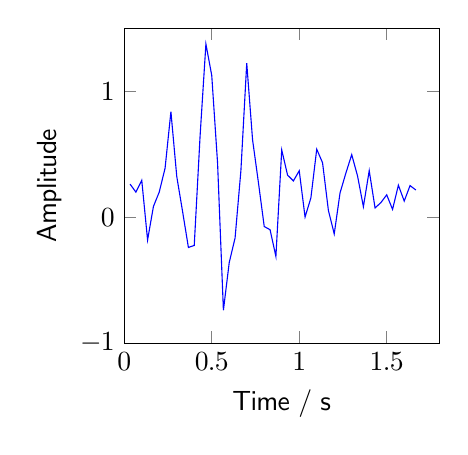
\begin{tikzpicture}

\begin{axis}[%
width=4cm,
height=4cm,
scale only axis,
xmin=0,
xmax=1.8,
xlabel={Time / s},
ymin=-1,
ymax=1.5,
ylabel={Amplitude}
]
\addplot [
color=blue,
solid,
forget plot
]
table[row sep=crcr]{
0.0333333333333333 0.262572613691037\\
0.0666666666666667 0.198860661196851\\
0.1 0.293247752491229\\
0.133333333333333 -0.180959372176469\\
0.166666666666667 0.0845586981331489\\
0.2 0.199854068088128\\
0.233333333333333 0.389259190729407\\
0.266666666666667 0.837919095709482\\
0.3 0.32429909668124\\
0.333333333333333 0.0452705760429178\\
0.366666666666667 -0.240197492370434\\
0.4 -0.224047548060361\\
0.433333333333333 0.643497283761552\\
0.466666666666667 1.37453362963137\\
0.5 1.12544841212521\\
0.533333333333333 0.428913122926589\\
0.566666666666667 -0.73830187863988\\
0.6 -0.359484987796598\\
0.633333333333333 -0.165033912302127\\
0.666666666666667 0.36992437648974\\
0.7 1.22217495509211\\
0.733333333333333 0.614363318746325\\
0.766666666666667 0.276350751805895\\
0.8 -0.0741571661575956\\
0.833333333333333 -0.0994119522959091\\
0.866666666666667 -0.31140109600246\\
0.9 0.533909441982054\\
0.933333333333333 0.334118655930567\\
0.966666666666667 0.288078537009979\\
1 0.36842112247229\\
1.03333333333333 0.00118474660706386\\
1.06666666666667 0.153611768817355\\
1.1 0.539723599007511\\
1.13333333333333 0.431913889589271\\
1.16666666666667 0.0538753495113479\\
1.2 -0.132553420774714\\
1.23333333333333 0.193258298798218\\
1.26666666666667 0.350514311002141\\
1.3 0.496461478741476\\
1.33333333333333 0.326831607857435\\
1.36666666666667 0.0836167421567026\\
1.4 0.369285371975842\\
1.43333333333333 0.0735755100960107\\
1.46666666666667 0.115848354359245\\
1.5 0.17729627218734\\
1.53333333333333 0.0621654242411572\\
1.56666666666667 0.253851271749024\\
1.6 0.128054218496774\\
1.63333333333333 0.250906957044431\\
1.66666666666667 0.215559864789581\\
};
\end{axis}
\end{tikzpicture}%

\caption{An example heartbeat simulated from the model.}
\label{fig:sineha_example_beat}
\end{figure}

The latent state is,
%
\begin{IEEEeqnarray}{rCl}
 \ls{\ti} & = & \begin{bmatrix} \amp{\ti} & \wid{\ti} & \del{\ti} & \freq{\ti} & \pha{\ti} & \bias{\ti} \end{bmatrix}^T      .
\end{IEEEeqnarray}
%
The transition density is factorised into independent terms, with $\freq{\ti}$, $\pha{\ti}$ and $\bias{\ti}$ evolving according to a Gaussian random walk, and $\wid{\ti}$ according to a geometric random walk (i.e. with a log-normal density), while $\del{\ti}$ and $\amp{\ti}$ are gamma distributed with no dependence on their past values. The resulting likelihood and filtering densities are highly multi-modal.





\subsection{Results}

Figures~\ref{fig:drone_example_frame_deterministic} and \ref{fig:sineha_example_frame} show the motion of the particles from the GFPF on a typical frame, and the awkward shapes of the posterior mode. Tables~\ref{tab:drone_results} and \ref{tab:sineha_results} show the average ESSs and RMSEs for each algorithm over 100 simulated data sets, each of 100 time steps.

\begin{figure}
\centering
% This file was created by matlab2tikz v0.4.4 running on MATLAB 7.13.
% Copyright (c) 2008--2013, Nico Schlömer <nico.schloemer@gmail.com>
% All rights reserved.
% 
% The latest updates can be retrieved from
%   http://www.mathworks.com/matlabcentral/fileexchange/22022-matlab2tikz
% where you can also make suggestions and rate matlab2tikz.
% 
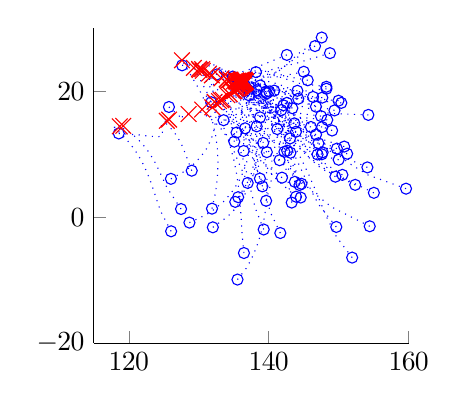
\begin{tikzpicture}

\begin{axis}[%
width=4cm,
height=4cm,
scale only axis,
xmin=115,
xmax=160,
ymin=-20,
ymax=30,
axis x line*=bottom,
axis y line*=left
]
\addplot [
color=blue,
dotted,
forget plot
]
table[row sep=crcr]{
155.018690286198 3.86922545662491\\
149.425467268873 6.860822463387\\
146.750015105775 9.32602893993351\\
144.979597310176 11.2910346237236\\
143.436687689586 13.07489413511\\
142.060362512987 14.6187324539903\\
140.767924452889 15.9772810742823\\
139.565897139671 17.1483849873456\\
138.462968959106 18.147301439957\\
137.486925750454 18.9749671194369\\
136.673293722738 19.6228236859888\\
136.068061958644 20.0738596044725\\
135.724827535481 20.3448688782558\\
135.697035803954 20.4725588121617\\
135.713721657807 20.5128608860202\\
};
\addplot [
color=blue,
only marks,
mark=o,
mark options={solid},
forget plot
]
table[row sep=crcr]{
155.018690286198 3.86922545662491\\
};
\addplot [
color=red,
mark size=4.0pt,
only marks,
mark=x,
mark options={solid},
forget plot
]
table[row sep=crcr]{
135.713721657807 20.5128608860202\\
};
\addplot [
color=blue,
dotted,
forget plot
]
table[row sep=crcr]{
150.781773601487 11.2092805073525\\
146.059193958141 12.9580482543366\\
144.398074841319 14.2171819613803\\
142.570026998153 15.8996711748458\\
141.325756817623 17.0841167620245\\
140.085083303452 18.2143073989427\\
139.019763206809 19.1305533230875\\
138.07601257223 19.9028484163764\\
137.313340600179 20.5017872776251\\
136.764090801283 20.9156906717331\\
136.463087826519 21.1493186154015\\
136.422379542842 21.2371721579975\\
136.426072989646 21.2628254396622\\
};
\addplot [
color=blue,
only marks,
mark=o,
mark options={solid},
forget plot
]
table[row sep=crcr]{
150.781773601487 11.2092805073525\\
};
\addplot [
color=red,
mark size=4.0pt,
only marks,
mark=x,
mark options={solid},
forget plot
]
table[row sep=crcr]{
136.426072989646 21.2628254396622\\
};
\addplot [
color=blue,
dotted,
forget plot
]
table[row sep=crcr]{
131.781747231719 18.2443284390259\\
131.249386917726 19.6487124694746\\
130.960136541985 19.4892656937001\\
131.324856874138 18.7118765089525\\
131.846668248869 18.2787742336233\\
132.155371857681 18.2849035730909\\
132.259689519306 18.3160362534253\\
};
\addplot [
color=blue,
only marks,
mark=o,
mark options={solid},
forget plot
]
table[row sep=crcr]{
131.781747231719 18.2443284390259\\
};
\addplot [
color=red,
mark size=4.0pt,
only marks,
mark=x,
mark options={solid},
forget plot
]
table[row sep=crcr]{
132.259689519306 18.3160362534253\\
};
\addplot [
color=blue,
dotted,
forget plot
]
table[row sep=crcr]{
125.736797402901 17.4963050402304\\
127.691363873998 15.5867118966465\\
127.680370006857 15.7126020721776\\
127.651162800425 16.0977737663762\\
127.969293566355 16.214804014546\\
128.355924272006 16.3219212505325\\
128.548324592513 16.3847322507276\\
};
\addplot [
color=blue,
only marks,
mark=o,
mark options={solid},
forget plot
]
table[row sep=crcr]{
125.736797402901 17.4963050402304\\
};
\addplot [
color=red,
mark size=4.0pt,
only marks,
mark=x,
mark options={solid},
forget plot
]
table[row sep=crcr]{
128.548324592513 16.3847322507276\\
};
\addplot [
color=blue,
dotted,
forget plot
]
table[row sep=crcr]{
139.202212446343 11.7930075274959\\
138.990451946785 14.9646662950337\\
138.607123914998 16.2249033801726\\
137.849261838772 17.7854687094008\\
137.166250730048 18.8167155704315\\
136.4788117007 19.7180212528745\\
135.920072257935 20.4201579084046\\
135.500042151141 20.9705386502933\\
135.237535281864 21.3502241665097\\
135.079925639153 21.5271177448825\\
135.017413984917 21.5594915133136\\
};
\addplot [
color=blue,
only marks,
mark=o,
mark options={solid},
forget plot
]
table[row sep=crcr]{
139.202212446343 11.7930075274959\\
};
\addplot [
color=red,
mark size=4.0pt,
only marks,
mark=x,
mark options={solid},
forget plot
]
table[row sep=crcr]{
135.017413984917 21.5594915133136\\
};
\addplot [
color=blue,
dotted,
forget plot
]
table[row sep=crcr]{
142.592288525256 18.1530630421389\\
138.310676513939 19.0959528124994\\
137.115866909268 19.8614614904633\\
135.399656199497 21.2567586516164\\
134.720186100706 21.8603431301339\\
134.194190514376 22.3204182966928\\
134.261515373333 22.2139080820846\\
134.526071022507 21.90340356829\\
134.528456309406 21.8436667183412\\
134.520260547223 21.8375861429981\\
};
\addplot [
color=blue,
only marks,
mark=o,
mark options={solid},
forget plot
]
table[row sep=crcr]{
142.592288525256 18.1530630421389\\
};
\addplot [
color=red,
mark size=4.0pt,
only marks,
mark=x,
mark options={solid},
forget plot
]
table[row sep=crcr]{
134.520260547223 21.8375861429981\\
};
\addplot [
color=blue,
dotted,
forget plot
]
table[row sep=crcr]{
146.022820016883 14.3246993619856\\
141.886061093836 15.7828766175245\\
140.561194357161 16.8526396622174\\
138.89294590432 18.5058744417163\\
137.956001150583 19.4799011318185\\
137.01815222345 20.4345293950706\\
136.331459423809 21.1184349205266\\
135.861959108506 21.5822541742874\\
135.707188403222 21.7355091496237\\
135.713644917568 21.6885582756249\\
135.688887715238 21.6742466152696\\
};
\addplot [
color=blue,
only marks,
mark=o,
mark options={solid},
forget plot
]
table[row sep=crcr]{
146.022820016883 14.3246993619856\\
};
\addplot [
color=red,
mark size=4.0pt,
only marks,
mark=x,
mark options={solid},
forget plot
]
table[row sep=crcr]{
135.688887715238 21.6742466152696\\
};
\addplot [
color=blue,
dotted,
forget plot
]
table[row sep=crcr]{
138.273918204626 14.4208853916693\\
135.898810959805 16.7962967428733\\
135.206001584595 17.2568082606875\\
134.064443903321 17.7946858627908\\
133.328247528421 18.0502241497767\\
132.818361728817 18.1890698696603\\
132.682945452625 18.279252017273\\
132.822386959336 18.3872455251997\\
132.885461909225 18.4305560386251\\
};
\addplot [
color=blue,
only marks,
mark=o,
mark options={solid},
forget plot
]
table[row sep=crcr]{
138.273918204626 14.4208853916693\\
};
\addplot [
color=red,
mark size=4.0pt,
only marks,
mark=x,
mark options={solid},
forget plot
]
table[row sep=crcr]{
132.885461909225 18.4305560386251\\
};
\addplot [
color=blue,
dotted,
forget plot
]
table[row sep=crcr]{
147.696671982024 10.2945623773545\\
143.629489093186 13.6540782290017\\
141.67942708566 16.1084798906001\\
140.317946617779 17.8445558926739\\
139.040509558226 19.3113307193436\\
137.91569716417 20.4007925097105\\
136.907675296566 21.1790581083882\\
136.096492943854 21.608019624952\\
135.594321890518 21.6175974992519\\
135.545531904719 21.1766972626078\\
135.684829788155 20.9891199104614\\
135.748006080416 20.9841697792913\\
};
\addplot [
color=blue,
only marks,
mark=o,
mark options={solid},
forget plot
]
table[row sep=crcr]{
147.696671982024 10.2945623773545\\
};
\addplot [
color=red,
mark size=4.0pt,
only marks,
mark=x,
mark options={solid},
forget plot
]
table[row sep=crcr]{
135.748006080416 20.9841697792913\\
};
\addplot [
color=blue,
dotted,
forget plot
]
table[row sep=crcr]{
138.276127523603 20.1618915578107\\
136.603843033344 21.6934989546234\\
136.110829876982 22.1893957237094\\
135.756045918939 22.4327875634506\\
136.008827471654 22.0899916772585\\
136.207160759164 21.8476993105337\\
136.22544552945 21.8052238765102\\
};
\addplot [
color=blue,
only marks,
mark=o,
mark options={solid},
forget plot
]
table[row sep=crcr]{
138.276127523603 20.1618915578107\\
};
\addplot [
color=red,
mark size=4.0pt,
only marks,
mark=x,
mark options={solid},
forget plot
]
table[row sep=crcr]{
136.22544552945 21.8052238765102\\
};
\addplot [
color=blue,
dotted,
forget plot
]
table[row sep=crcr]{
141.545488776135 9.04505288371162\\
140.386961095056 12.465944058757\\
139.757503737479 14.4297208931264\\
138.948516208705 16.3960530019496\\
138.124946677111 17.8531457996504\\
137.211116288795 19.0370046796853\\
136.339272872886 19.8675027736354\\
135.599986768596 20.36911355549\\
135.131943983233 20.5138740011154\\
135.044993896517 20.3577918832202\\
135.158499010878 20.3431443692921\\
135.218570598087 20.3703822381972\\
};
\addplot [
color=blue,
only marks,
mark=o,
mark options={solid},
forget plot
]
table[row sep=crcr]{
141.545488776135 9.04505288371162\\
};
\addplot [
color=red,
mark size=4.0pt,
only marks,
mark=x,
mark options={solid},
forget plot
]
table[row sep=crcr]{
135.218570598087 20.3703822381972\\
};
\addplot [
color=blue,
dotted,
forget plot
]
table[row sep=crcr]{
135.626716518387 3.17709452175102\\
137.100577324009 5.70690532592245\\
137.601431764466 7.23371625302858\\
138.04074327591 9.46617308885846\\
138.182648908254 11.3872025659319\\
138.124615889016 13.3466020329551\\
137.890826506972 15.1201273075458\\
137.520899342262 16.7526674441315\\
137.083507822064 18.1865170727285\\
136.656088580283 19.4114424936628\\
136.325732149185 20.3998842465847\\
136.170880712226 21.1101874138992\\
136.194897089929 21.4985621275013\\
136.202796695306 21.5685881854796\\
136.196356657804 21.5789353092994\\
};
\addplot [
color=blue,
only marks,
mark=o,
mark options={solid},
forget plot
]
table[row sep=crcr]{
135.626716518387 3.17709452175102\\
};
\addplot [
color=red,
mark size=4.0pt,
only marks,
mark=x,
mark options={solid},
forget plot
]
table[row sep=crcr]{
136.196356657804 21.5789353092994\\
};
\addplot [
color=blue,
dotted,
forget plot
]
table[row sep=crcr]{
144.666859367104 5.30628079222142\\
142.876549418503 8.58769396681524\\
142.051120437635 10.8502214892657\\
141.258004880023 12.9916727434767\\
140.4795933333 14.8296763083249\\
139.660788252476 16.4703172166092\\
138.840536398397 17.8776241972241\\
138.051739434839 19.0749599193507\\
137.346110531929 20.0633352140659\\
136.777121582146 20.83517260858\\
136.406129434342 21.3558405425875\\
136.254975023676 21.5976893314962\\
136.216852893126 21.6281774223248\\
136.201183665897 21.6310964251117\\
};
\addplot [
color=blue,
only marks,
mark=o,
mark options={solid},
forget plot
]
table[row sep=crcr]{
144.666859367104 5.30628079222142\\
};
\addplot [
color=red,
mark size=4.0pt,
only marks,
mark=x,
mark options={solid},
forget plot
]
table[row sep=crcr]{
136.201183665897 21.6310964251117\\
};
\addplot [
color=blue,
dotted,
forget plot
]
table[row sep=crcr]{
159.613445291932 4.52839434835128\\
154.172144265848 6.71380964861869\\
151.494653263324 8.54834906146826\\
149.298563387061 10.4328179659785\\
147.645194382647 11.9720328905705\\
146.112842822494 13.3963936146516\\
144.723126555575 14.6410095384009\\
143.411196602204 15.7608909349462\\
142.183848169883 16.7636553170035\\
141.03546647757 17.6713895448938\\
139.972118313772 18.4943890593484\\
138.99993827676 19.2385876394602\\
138.129995273584 19.9015379599555\\
137.377672630813 20.473227129704\\
136.761668598454 20.9367210694727\\
136.289411692869 21.2728475297782\\
136.074197028199 21.3962692114087\\
136.040821525467 21.4113309124747\\
};
\addplot [
color=blue,
only marks,
mark=o,
mark options={solid},
forget plot
]
table[row sep=crcr]{
159.613445291932 4.52839434835128\\
};
\addplot [
color=red,
mark size=4.0pt,
only marks,
mark=x,
mark options={solid},
forget plot
]
table[row sep=crcr]{
136.040821525467 21.4113309124747\\
};
\addplot [
color=blue,
dotted,
forget plot
]
table[row sep=crcr]{
149.049919032442 13.759500239734\\
144.376005643139 15.7705889461781\\
142.59450078959 17.1340407137271\\
140.926267116576 18.4517311747244\\
139.711241215379 19.3177181758362\\
138.576264597423 20.0140449173113\\
137.635561171924 20.4996916393279\\
136.87863742904 20.8143909689013\\
136.364068390234 20.9599465326532\\
136.114982001568 20.9894831937163\\
136.112152905383 21.0308084144198\\
136.135815382312 21.0603731250043\\
};
\addplot [
color=blue,
only marks,
mark=o,
mark options={solid},
forget plot
]
table[row sep=crcr]{
149.049919032442 13.759500239734\\
};
\addplot [
color=red,
mark size=4.0pt,
only marks,
mark=x,
mark options={solid},
forget plot
]
table[row sep=crcr]{
136.135815382312 21.0603731250043\\
};
\addplot [
color=blue,
dotted,
forget plot
]
table[row sep=crcr]{
141.650566946275 -2.51079787487569\\
140.336590288147 0.51755321938533\\
139.678667574236 2.7528131907701\\
139.0498243107 5.06569203463662\\
138.443687118474 7.14911031091844\\
137.780067670871 9.14216286419526\\
137.061557531363 10.9759871518342\\
136.286579651089 12.6611018588591\\
135.489557641804 14.1720663315581\\
134.720825267294 15.4962526041361\\
134.046346607959 16.6139176884584\\
133.535033148214 17.4973994376879\\
133.252292527954 18.1222829596224\\
133.307676893103 18.5009530361987\\
133.414462590396 18.6250429541817\\
};
\addplot [
color=blue,
only marks,
mark=o,
mark options={solid},
forget plot
]
table[row sep=crcr]{
141.650566946275 -2.51079787487569\\
};
\addplot [
color=red,
mark size=4.0pt,
only marks,
mark=x,
mark options={solid},
forget plot
]
table[row sep=crcr]{
133.414462590396 18.6250429541817\\
};
\addplot [
color=blue,
dotted,
forget plot
]
table[row sep=crcr]{
141.204680478793 13.9901863277667\\
138.64351502309 16.5194412618105\\
138.163607178332 17.4282396585283\\
137.445070437552 18.7875948899796\\
136.992389832121 19.7082863021746\\
136.666671570577 20.5429374481347\\
136.524629575084 21.1455185305113\\
136.481740630589 21.4667279652261\\
136.466679728575 21.5130876584753\\
};
\addplot [
color=blue,
only marks,
mark=o,
mark options={solid},
forget plot
]
table[row sep=crcr]{
141.204680478793 13.9901863277667\\
};
\addplot [
color=red,
mark size=4.0pt,
only marks,
mark=x,
mark options={solid},
forget plot
]
table[row sep=crcr]{
136.466679728575 21.5130876584753\\
};
\addplot [
color=blue,
dotted,
forget plot
]
table[row sep=crcr]{
136.675611650948 20.7680309271502\\
135.020991109185 22.1473295098669\\
134.792228392811 22.6351454034726\\
135.319744496728 22.3799832562271\\
135.788200629645 22.0224878030726\\
135.992189678467 21.8398769788793\\
136.014039307201 21.8032662705093\\
};
\addplot [
color=blue,
only marks,
mark=o,
mark options={solid},
forget plot
]
table[row sep=crcr]{
136.675611650948 20.7680309271502\\
};
\addplot [
color=red,
mark size=4.0pt,
only marks,
mark=x,
mark options={solid},
forget plot
]
table[row sep=crcr]{
136.014039307201 21.8032662705093\\
};
\addplot [
color=blue,
dotted,
forget plot
]
table[row sep=crcr]{
148.243037077316 20.3931488490607\\
144.008036112954 19.8826855141507\\
142.763128419282 19.9579260769373\\
140.952901086685 20.2956279486007\\
139.776040325944 20.6512852140781\\
138.640577751576 21.0516863170305\\
137.766243644494 21.3728376439845\\
137.108791254038 21.5898371009928\\
136.729299362101 21.6620239115841\\
136.596550642388 21.6440434811092\\
136.584862025831 21.6448721345904\\
};
\addplot [
color=blue,
only marks,
mark=o,
mark options={solid},
forget plot
]
table[row sep=crcr]{
148.243037077316 20.3931488490607\\
};
\addplot [
color=red,
mark size=4.0pt,
only marks,
mark=x,
mark options={solid},
forget plot
]
table[row sep=crcr]{
136.584862025831 21.6448721345904\\
};
\addplot [
color=blue,
dotted,
forget plot
]
table[row sep=crcr]{
139.623124667585 2.60250437976515\\
140.288026523535 5.30014535714969\\
140.436451420636 6.85292354386164\\
140.449907181097 9.01410076307193\\
140.27284299445 10.8796676052749\\
139.906569908527 12.7664182237056\\
139.395197407417 14.4858979666672\\
138.776420287367 16.0675505726671\\
138.127840129469 17.4664208783658\\
137.517007195905 18.6792241202885\\
137.006933542814 19.6871615258602\\
136.645630041904 20.4607429390694\\
136.463429973614 20.9808976966847\\
136.453770492349 21.1323043783121\\
136.455786445597 21.151849749611\\
};
\addplot [
color=blue,
only marks,
mark=o,
mark options={solid},
forget plot
]
table[row sep=crcr]{
139.623124667585 2.60250437976515\\
};
\addplot [
color=red,
mark size=4.0pt,
only marks,
mark=x,
mark options={solid},
forget plot
]
table[row sep=crcr]{
136.455786445597 21.151849749611\\
};
\addplot [
color=blue,
dotted,
forget plot
]
table[row sep=crcr]{
149.73129515491 10.8866259134494\\
145.438550717059 12.9427354909872\\
143.937455802091 14.2952063720046\\
142.286896140457 15.9765203195219\\
141.056829094508 17.1918575978736\\
139.820239288832 18.3055727316891\\
138.727232029702 19.1953580863058\\
137.756249807804 19.9159203160981\\
136.973159303696 20.443796126759\\
136.422909092997 20.7690748044802\\
136.151446436839 20.9276037805848\\
136.146350362609 20.9963191083251\\
136.154774494136 21.0144083693612\\
};
\addplot [
color=blue,
only marks,
mark=o,
mark options={solid},
forget plot
]
table[row sep=crcr]{
149.73129515491 10.8866259134494\\
};
\addplot [
color=red,
mark size=4.0pt,
only marks,
mark=x,
mark options={solid},
forget plot
]
table[row sep=crcr]{
136.154774494136 21.0144083693612\\
};
\addplot [
color=blue,
dotted,
forget plot
]
table[row sep=crcr]{
149.961703450098 18.4936695619146\\
146.198001248989 18.8435662595776\\
144.964232494343 19.2159359227125\\
143.270674443718 19.7345623501749\\
142.045546190911 20.080009241656\\
140.817448410942 20.4004824167835\\
139.759266542618 20.6701956639306\\
138.8145953277 20.911331088515\\
138.020047280288 21.1173938798598\\
137.388007869288 21.2858778486676\\
136.944578928663 21.4139662895592\\
136.774631330989 21.4830303802529\\
136.746244099684 21.5010611737043\\
};
\addplot [
color=blue,
only marks,
mark=o,
mark options={solid},
forget plot
]
table[row sep=crcr]{
149.961703450098 18.4936695619146\\
};
\addplot [
color=red,
mark size=4.0pt,
only marks,
mark=x,
mark options={solid},
forget plot
]
table[row sep=crcr]{
136.746244099684 21.5010611737043\\
};
\addplot [
color=blue,
dotted,
forget plot
]
table[row sep=crcr]{
144.088149585833 20.065869932542\\
140.935886641141 20.586521927969\\
140.076212786325 20.876270216113\\
138.833968878565 21.196970484181\\
138.036652363176 21.3595909490375\\
137.351670382951 21.470841979743\\
136.913433824499 21.5275539195841\\
136.676795919114 21.5680748310673\\
136.622490690105 21.5933824191537\\
136.611744750686 21.601883668197\\
};
\addplot [
color=blue,
only marks,
mark=o,
mark options={solid},
forget plot
]
table[row sep=crcr]{
144.088149585833 20.065869932542\\
};
\addplot [
color=red,
mark size=4.0pt,
only marks,
mark=x,
mark options={solid},
forget plot
]
table[row sep=crcr]{
136.611744750686 21.601883668197\\
};
\addplot [
color=blue,
dotted,
forget plot
]
table[row sep=crcr]{
143.898618076493 3.25196916474037\\
140.610501355101 6.5281968093322\\
139.209529089579 8.75556552263765\\
138.051316687245 10.7695404158797\\
137.013233325009 12.5119165277804\\
136.009271613173 14.0500484537754\\
135.057834580748 15.3641605841686\\
134.199781422335 16.4586241622293\\
133.509045523695 17.3206622314193\\
133.064170037698 17.9310914166372\\
132.942068360236 18.3126440595381\\
133.095706664459 18.4996843787854\\
133.182639811545 18.5715713543474\\
};
\addplot [
color=blue,
only marks,
mark=o,
mark options={solid},
forget plot
]
table[row sep=crcr]{
143.898618076493 3.25196916474037\\
};
\addplot [
color=red,
mark size=4.0pt,
only marks,
mark=x,
mark options={solid},
forget plot
]
table[row sep=crcr]{
133.182639811545 18.5715713543474\\
};
\addplot [
color=blue,
dotted,
forget plot
]
table[row sep=crcr]{
147.583956192726 9.98909257121404\\
143.935564574459 12.3314092333461\\
142.70816521955 13.7808334114326\\
141.392666962389 15.4371683979768\\
140.343640148699 16.6843451814875\\
139.301074447914 17.8288067180317\\
138.378889694458 18.7831355774507\\
137.577859159354 19.5942633696925\\
136.949739708304 20.242690334526\\
136.525931909413 20.7143053313607\\
136.344551443126 21.0227698580645\\
136.348528822263 21.0936153048855\\
};
\addplot [
color=blue,
only marks,
mark=o,
mark options={solid},
forget plot
]
table[row sep=crcr]{
147.583956192726 9.98909257121404\\
};
\addplot [
color=red,
mark size=4.0pt,
only marks,
mark=x,
mark options={solid},
forget plot
]
table[row sep=crcr]{
136.348528822263 21.0936153048855\\
};
\addplot [
color=blue,
dotted,
forget plot
]
table[row sep=crcr]{
148.744061483126 26.0435900966758\\
144.069797338933 24.4873492360726\\
142.555300113744 24.0468619239729\\
140.520778677763 23.4571468080672\\
139.135025412057 23.037186647029\\
137.832227301296 22.5851353028919\\
136.823628509993 22.1413953266478\\
136.081653365523 21.6441109513733\\
135.673549326748 21.1174883057429\\
135.575312431178 20.7373367639302\\
135.637773694331 20.7218131352753\\
135.66362759962 20.7337345166041\\
};
\addplot [
color=blue,
only marks,
mark=o,
mark options={solid},
forget plot
]
table[row sep=crcr]{
148.744061483126 26.0435900966758\\
};
\addplot [
color=red,
mark size=4.0pt,
only marks,
mark=x,
mark options={solid},
forget plot
]
table[row sep=crcr]{
135.66362759962 20.7337345166041\\
};
\addplot [
color=blue,
dotted,
forget plot
]
table[row sep=crcr]{
154.230154366767 16.2409846427533\\
148.970403230933 16.4521422963381\\
147.019575571943 16.8608962041279\\
144.669635756465 17.5984689942541\\
143.042604651709 18.2152722996691\\
141.452521193482 18.8312361235254\\
140.078978640766 19.3463854438467\\
138.833413857517 19.785953140806\\
137.763785319899 20.1311593467459\\
136.887011417444 20.3739981854464\\
136.243634736418 20.5087407589413\\
135.878417926827 20.5798995625524\\
135.845323833733 20.6488958164468\\
135.854717400529 20.6725515143517\\
};
\addplot [
color=blue,
only marks,
mark=o,
mark options={solid},
forget plot
]
table[row sep=crcr]{
154.230154366767 16.2409846427533\\
};
\addplot [
color=red,
mark size=4.0pt,
only marks,
mark=x,
mark options={solid},
forget plot
]
table[row sep=crcr]{
135.854717400529 20.6725515143517\\
};
\addplot [
color=blue,
dotted,
forget plot
]
table[row sep=crcr]{
141.790022597945 17.0109903776414\\
139.165189950694 19.7011501875515\\
138.381276237463 20.6293957857546\\
137.327899213055 21.6175046636253\\
136.693416103503 22.0582090019799\\
136.313973808516 22.177080538655\\
136.361808020377 21.9117841862181\\
136.459063085392 21.764641159414\\
136.478143635796 21.7421643679652\\
};
\addplot [
color=blue,
only marks,
mark=o,
mark options={solid},
forget plot
]
table[row sep=crcr]{
141.790022597945 17.0109903776414\\
};
\addplot [
color=red,
mark size=4.0pt,
only marks,
mark=x,
mark options={solid},
forget plot
]
table[row sep=crcr]{
136.478143635796 21.7421643679652\\
};
\addplot [
color=blue,
dotted,
forget plot
]
table[row sep=crcr]{
150.367732833459 18.1486124195207\\
146.145186388261 18.5648382999335\\
144.74207434 19.0049079833667\\
142.902594289112 19.6281424753681\\
141.604474048301 20.0281473528038\\
140.299196782676 20.3734397668325\\
139.180476279859 20.6317789031085\\
138.194091657623 20.8298132158778\\
137.389883884746 20.9636222883886\\
136.788197048008 21.039354381154\\
136.424519412209 21.0880403412997\\
136.361477555827 21.1378602216653\\
136.360432889694 21.1548283959712\\
};
\addplot [
color=blue,
only marks,
mark=o,
mark options={solid},
forget plot
]
table[row sep=crcr]{
150.367732833459 18.1486124195207\\
};
\addplot [
color=red,
mark size=4.0pt,
only marks,
mark=x,
mark options={solid},
forget plot
]
table[row sep=crcr]{
136.360432889694 21.1548283959712\\
};
\addplot [
color=blue,
dotted,
forget plot
]
table[row sep=crcr]{
135.393833931034 13.4328069426672\\
136.286822954415 16.6516130706588\\
136.196241207619 17.7408640791479\\
135.811475702936 19.3209512498712\\
135.45546852666 20.3046725870267\\
135.201487559813 21.0807484140875\\
135.217157442173 21.5011722076526\\
135.367044543971 21.610204490189\\
135.364643830665 21.6185813739704\\
135.357384078736 21.6197016462069\\
};
\addplot [
color=blue,
only marks,
mark=o,
mark options={solid},
forget plot
]
table[row sep=crcr]{
135.393833931034 13.4328069426672\\
};
\addplot [
color=red,
mark size=4.0pt,
only marks,
mark=x,
mark options={solid},
forget plot
]
table[row sep=crcr]{
135.357384078736 21.6197016462069\\
};
\addplot [
color=blue,
dotted,
forget plot
]
table[row sep=crcr]{
132.597430337076 22.6637725616049\\
130.694061511622 22.9083430551055\\
130.159515590876 23.3937461555765\\
129.915890201975 23.6574229081048\\
130.073559627943 23.5420685868145\\
130.084762240523 23.5136214618467\\
130.038812473449 23.5347600411815\\
};
\addplot [
color=blue,
only marks,
mark=o,
mark options={solid},
forget plot
]
table[row sep=crcr]{
132.597430337076 22.6637725616049\\
};
\addplot [
color=red,
mark size=4.0pt,
only marks,
mark=x,
mark options={solid},
forget plot
]
table[row sep=crcr]{
130.038812473449 23.5347600411815\\
};
\addplot [
color=blue,
dotted,
forget plot
]
table[row sep=crcr]{
140.784376999147 20.0888588087893\\
137.731114110775 19.7729909892776\\
137.04755731023 19.9870758677148\\
135.773312168339 20.5760378149018\\
135.015712006028 21.0048701271137\\
134.293588673796 21.4421732385757\\
133.798000853683 21.7530660222874\\
133.49288965253 21.9400647084297\\
133.312560329074 22.0250451553334\\
133.239007853678 22.0512434700241\\
};
\addplot [
color=blue,
only marks,
mark=o,
mark options={solid},
forget plot
]
table[row sep=crcr]{
140.784376999147 20.0888588087893\\
};
\addplot [
color=red,
mark size=4.0pt,
only marks,
mark=x,
mark options={solid},
forget plot
]
table[row sep=crcr]{
133.239007853678 22.0512434700241\\
};
\addplot [
color=blue,
dotted,
forget plot
]
table[row sep=crcr]{
142.582797691797 25.7652804477649\\
138.991475189069 24.1403229560155\\
137.838796402261 23.6649456143482\\
136.210357126096 23.0719327652833\\
135.082441076988 22.794307761824\\
133.979190759699 22.6734559739048\\
133.119041808849 22.6862900097885\\
132.437533089653 22.7357890817527\\
131.976514198847 22.756546590816\\
131.711193393712 22.7443163988278\\
131.543428476687 22.7707977228518\\
131.463784413005 22.8012883998158\\
};
\addplot [
color=blue,
only marks,
mark=o,
mark options={solid},
forget plot
]
table[row sep=crcr]{
142.582797691797 25.7652804477649\\
};
\addplot [
color=red,
mark size=4.0pt,
only marks,
mark=x,
mark options={solid},
forget plot
]
table[row sep=crcr]{
131.463784413005 22.8012883998158\\
};
\addplot [
color=blue,
dotted,
forget plot
]
table[row sep=crcr]{
148.357356874611 15.4449113710782\\
144.328998220098 15.8597769801039\\
142.924139103394 16.4083088740921\\
141.016590331576 17.4746576475449\\
139.905044335812 18.2104054750532\\
138.779581872553 18.9864365395493\\
137.874988815794 19.6293927719819\\
137.082529991428 20.2130859061376\\
136.450852524541 20.7058821556746\\
135.982031970847 21.1047473513783\\
135.67408389727 21.3900451427681\\
135.515491017279 21.5047370070555\\
135.461237892338 21.5269780228627\\
};
\addplot [
color=blue,
only marks,
mark=o,
mark options={solid},
forget plot
]
table[row sep=crcr]{
148.357356874611 15.4449113710782\\
};
\addplot [
color=red,
mark size=4.0pt,
only marks,
mark=x,
mark options={solid},
forget plot
]
table[row sep=crcr]{
135.461237892338 21.5269780228627\\
};
\addplot [
color=blue,
dotted,
forget plot
]
table[row sep=crcr]{
147.089534785944 11.7349925216565\\
143.380596334866 13.4730748109939\\
142.127493632795 14.6920502382284\\
140.670294185488 16.3203833705763\\
139.683872352507 17.4208669927251\\
138.685917000915 18.4863108602474\\
137.839050747135 19.3610826144328\\
137.097847233677 20.1212447552073\\
136.512213851168 20.7365591551251\\
136.102670647952 21.1923594087338\\
135.859595077676 21.4665155824279\\
135.768713193299 21.5273557410385\\
135.745143594123 21.5363949791605\\
};
\addplot [
color=blue,
only marks,
mark=o,
mark options={solid},
forget plot
]
table[row sep=crcr]{
147.089534785944 11.7349925216565\\
};
\addplot [
color=red,
mark size=4.0pt,
only marks,
mark=x,
mark options={solid},
forget plot
]
table[row sep=crcr]{
135.745143594123 21.5363949791605\\
};
\addplot [
color=blue,
dotted,
forget plot
]
table[row sep=crcr]{
136.618522135894 14.1121496731477\\
137.425076572897 17.4157628222509\\
137.251672277221 18.4775480490028\\
136.6796089374 19.944684452696\\
136.161627993465 20.7921565760554\\
135.720311727366 21.4124658013721\\
135.545528615766 21.6947463219046\\
135.605571146906 21.6928694639387\\
135.600493704058 21.6682719341274\\
135.586041029406 21.6630580796305\\
};
\addplot [
color=blue,
only marks,
mark=o,
mark options={solid},
forget plot
]
table[row sep=crcr]{
136.618522135894 14.1121496731477\\
};
\addplot [
color=red,
mark size=4.0pt,
only marks,
mark=x,
mark options={solid},
forget plot
]
table[row sep=crcr]{
135.586041029406 21.6630580796305\\
};
\addplot [
color=blue,
dotted,
forget plot
]
table[row sep=crcr]{
143.277370484227 2.32353884973139\\
142.819654609582 5.23066395543165\\
142.562833275162 7.05781251799597\\
142.164590806293 9.28661555724661\\
141.690380976068 11.2003918302124\\
141.074387889131 13.0671493532227\\
140.370493306094 14.7405935308939\\
139.60623019402 16.254033443271\\
138.843623762217 17.5872915579467\\
138.128256100612 18.7526577667953\\
137.503965650748 19.7462310135093\\
137.008521888574 20.5500998854598\\
136.667905088523 21.130957600365\\
136.494335649357 21.4133956179527\\
136.452921738823 21.4605962632211\\
};
\addplot [
color=blue,
only marks,
mark=o,
mark options={solid},
forget plot
]
table[row sep=crcr]{
143.277370484227 2.32353884973139\\
};
\addplot [
color=red,
mark size=4.0pt,
only marks,
mark=x,
mark options={solid},
forget plot
]
table[row sep=crcr]{
136.452921738823 21.4605962632211\\
};
\addplot [
color=blue,
dotted,
forget plot
]
table[row sep=crcr]{
146.744254415129 17.5513711796577\\
143.681332907512 18.8745028472064\\
142.634666719791 19.545083982831\\
141.22816713476 20.284498653006\\
140.145894375483 20.7258754261556\\
139.083827160759 21.0737810040637\\
138.19478781493 21.3082980359274\\
137.470591644998 21.449325523172\\
136.959030013427 21.5035698165648\\
136.673916468005 21.5151921697273\\
136.632260029709 21.5310435251004\\
136.629565536066 21.533623013042\\
};
\addplot [
color=blue,
only marks,
mark=o,
mark options={solid},
forget plot
]
table[row sep=crcr]{
146.744254415129 17.5513711796577\\
};
\addplot [
color=red,
mark size=4.0pt,
only marks,
mark=x,
mark options={solid},
forget plot
]
table[row sep=crcr]{
136.629565536066 21.533623013042\\
};
\addplot [
color=blue,
dotted,
forget plot
]
table[row sep=crcr]{
134.865681999761 22.3235975747527\\
135.157898282507 20.4806607400284\\
135.356984155819 20.743565800391\\
135.679726491126 21.2677236719111\\
135.852529060806 21.503074826045\\
135.84121671752 21.5383641278696\\
135.83875206974 21.5401004130664\\
};
\addplot [
color=blue,
only marks,
mark=o,
mark options={solid},
forget plot
]
table[row sep=crcr]{
134.865681999761 22.3235975747527\\
};
\addplot [
color=red,
mark size=4.0pt,
only marks,
mark=x,
mark options={solid},
forget plot
]
table[row sep=crcr]{
135.83875206974 21.5401004130664\\
};
\addplot [
color=blue,
dotted,
forget plot
]
table[row sep=crcr]{
146.608717764415 27.1669435418587\\
143.354929752632 24.8688291755382\\
142.482818483644 24.1111672335268\\
141.000281428624 23.0084793522322\\
139.825553236454 22.5196342034883\\
138.698496387018 22.2863562748426\\
137.80118307098 22.1746477264391\\
137.113722419976 22.0601056802304\\
136.677367375776 21.9050589344037\\
136.463182402384 21.7710457739184\\
136.416224273027 21.7454373148686\\
};
\addplot [
color=blue,
only marks,
mark=o,
mark options={solid},
forget plot
]
table[row sep=crcr]{
146.608717764415 27.1669435418587\\
};
\addplot [
color=red,
mark size=4.0pt,
only marks,
mark=x,
mark options={solid},
forget plot
]
table[row sep=crcr]{
136.416224273027 21.7454373148686\\
};
\addplot [
color=blue,
dotted,
forget plot
]
table[row sep=crcr]{
147.646777935643 18.9838403465986\\
143.265708734353 18.8274739068691\\
141.976940725513 19.0857876935811\\
140.044225048207 19.8521006353943\\
138.891995644547 20.5031013422119\\
137.77067048427 21.1968709781444\\
136.957918899533 21.6931485235087\\
136.401343281308 21.9672456214751\\
136.205630657943 21.9159700025931\\
136.201588804646 21.7852083938387\\
136.187072991501 21.7562741844253\\
};
\addplot [
color=blue,
only marks,
mark=o,
mark options={solid},
forget plot
]
table[row sep=crcr]{
147.646777935643 18.9838403465986\\
};
\addplot [
color=red,
mark size=4.0pt,
only marks,
mark=x,
mark options={solid},
forget plot
]
table[row sep=crcr]{
136.187072991501 21.7562741844253\\
};
\addplot [
color=blue,
dotted,
forget plot
]
table[row sep=crcr]{
149.986395133634 9.1218695037554\\
145.246415728344 10.3309965882301\\
143.801950603435 11.2927691762843\\
141.892078979666 13.2367670978722\\
140.800318040589 14.6471725552674\\
139.699119645834 16.1819568474798\\
138.786648954397 17.5014581906864\\
137.978956434609 18.7152171265657\\
137.336892293266 19.7488140468187\\
136.884388559747 20.5726896269739\\
136.640473901143 21.1311246732363\\
136.590980173254 21.3249003935592\\
136.586859077579 21.3654768127285\\
};
\addplot [
color=blue,
only marks,
mark=o,
mark options={solid},
forget plot
]
table[row sep=crcr]{
149.986395133634 9.1218695037554\\
};
\addplot [
color=red,
mark size=4.0pt,
only marks,
mark=x,
mark options={solid},
forget plot
]
table[row sep=crcr]{
136.586859077579 21.3654768127285\\
};
\addplot [
color=blue,
dotted,
forget plot
]
table[row sep=crcr]{
151.916884700738 -6.4132750959162\\
149.689015337081 -3.1365719188538\\
148.422299789948 -0.35979946549695\\
147.45294598211 2.16454063194071\\
146.571006187871 4.54803041423763\\
145.702354455093 6.78637090205276\\
144.803986992015 8.88739523718417\\
143.861242797619 10.8403107486394\\
142.875843461103 12.6375094161594\\
141.865323106394 14.2721337328798\\
140.856449080504 15.7435761476464\\
139.879773120418 17.0554721130281\\
138.96623988523 18.2110173081268\\
138.147923101429 19.2064010168764\\
137.460149136051 20.0263650861566\\
136.940968763503 20.6474697305237\\
136.630568270678 21.0683531536471\\
136.587168995912 21.1773192849233\\
};
\addplot [
color=blue,
only marks,
mark=o,
mark options={solid},
forget plot
]
table[row sep=crcr]{
151.916884700738 -6.4132750959162\\
};
\addplot [
color=red,
mark size=4.0pt,
only marks,
mark=x,
mark options={solid},
forget plot
]
table[row sep=crcr]{
136.587168995912 21.1773192849233\\
};
\addplot [
color=blue,
dotted,
forget plot
]
table[row sep=crcr]{
135.0702591319 11.9905249577565\\
134.75515442245 15.2670118065602\\
134.667270981656 16.4882886925544\\
134.566508164329 18.1739806005413\\
134.5991895294 19.3504125652761\\
134.901986670817 20.2919444593217\\
135.458782131225 20.8079176111934\\
135.885275736621 21.0205938636509\\
136.021240862793 21.1011554735233\\
136.036336517009 21.1114126800658\\
};
\addplot [
color=blue,
only marks,
mark=o,
mark options={solid},
forget plot
]
table[row sep=crcr]{
135.0702591319 11.9905249577565\\
};
\addplot [
color=red,
mark size=4.0pt,
only marks,
mark=x,
mark options={solid},
forget plot
]
table[row sep=crcr]{
136.036336517009 21.1114126800658\\
};
\addplot [
color=blue,
dotted,
forget plot
]
table[row sep=crcr]{
118.567112153678 13.2963972764718\\
121.743502200704 13.0257481889168\\
122.895442115578 12.8660097485381\\
124.214546148513 12.754807939304\\
124.788251647305 12.9885347010446\\
124.812365353596 13.6663460420661\\
124.658375029961 14.3652958529088\\
124.686488448832 14.8922826548103\\
125.114209224872 15.1970485765469\\
125.433087514437 15.3039125398164\\
};
\addplot [
color=blue,
only marks,
mark=o,
mark options={solid},
forget plot
]
table[row sep=crcr]{
118.567112153678 13.2963972764718\\
};
\addplot [
color=red,
mark size=4.0pt,
only marks,
mark=x,
mark options={solid},
forget plot
]
table[row sep=crcr]{
125.433087514437 15.3039125398164\\
};
\addplot [
color=blue,
dotted,
forget plot
]
table[row sep=crcr]{
139.57991989093 19.8975168735818\\
137.596075928481 20.691678861658\\
136.846075592242 20.7251148931417\\
135.847918144826 20.6370959511587\\
135.248397194289 20.453767734525\\
134.910762359128 20.1800611529076\\
134.917348233546 20.0680634959964\\
134.993857523881 20.1087841421941\\
};
\addplot [
color=blue,
only marks,
mark=o,
mark options={solid},
forget plot
]
table[row sep=crcr]{
139.57991989093 19.8975168735818\\
};
\addplot [
color=red,
mark size=4.0pt,
only marks,
mark=x,
mark options={solid},
forget plot
]
table[row sep=crcr]{
134.993857523881 20.1087841421941\\
};
\addplot [
color=blue,
dotted,
forget plot
]
table[row sep=crcr]{
143.040113264599 12.5043435520551\\
141.247966750615 15.5228514257562\\
140.43101581841 16.9766972814498\\
139.473934559718 18.3095256841229\\
138.650707673932 19.213794690849\\
137.860040399271 19.9504011379439\\
137.191315269716 20.5149965801713\\
136.656276513367 20.9527733577009\\
136.282898910742 21.2725992773766\\
136.050760450544 21.4827230199141\\
135.957678943494 21.5360849326554\\
135.930775355066 21.5447020673692\\
};
\addplot [
color=blue,
only marks,
mark=o,
mark options={solid},
forget plot
]
table[row sep=crcr]{
143.040113264599 12.5043435520551\\
};
\addplot [
color=red,
mark size=4.0pt,
only marks,
mark=x,
mark options={solid},
forget plot
]
table[row sep=crcr]{
135.930775355066 21.5447020673692\\
};
\addplot [
color=blue,
dotted,
forget plot
]
table[row sep=crcr]{
144.56453229523 3.12112913813375\\
144.052322603992 6.16889140383825\\
143.748515536326 8.22641764001906\\
143.297056132336 10.5165801766594\\
142.745558530957 12.464790914745\\
142.030803133028 14.2932392748872\\
141.20735901667 15.8822233046792\\
140.309340935687 17.2631942747588\\
139.404387969692 18.4333520035669\\
138.540421240874 19.4178886195979\\
137.761138347041 20.2274273487888\\
137.106520359215 20.8582395614604\\
136.61638578222 21.2929354001323\\
136.301954867258 21.5260681766333\\
136.194196136028 21.5724566753274\\
136.173719778752 21.5776098348617\\
};
\addplot [
color=blue,
only marks,
mark=o,
mark options={solid},
forget plot
]
table[row sep=crcr]{
144.56453229523 3.12112913813375\\
};
\addplot [
color=red,
mark size=4.0pt,
only marks,
mark=x,
mark options={solid},
forget plot
]
table[row sep=crcr]{
136.173719778752 21.5776098348617\\
};
\addplot [
color=blue,
dotted,
forget plot
]
table[row sep=crcr]{
141.890712529927 6.27869589606682\\
138.464871696552 9.31265717444816\\
137.421392051212 11.0800461036959\\
136.467229110242 12.9772505755462\\
135.705127217689 14.5672170347394\\
135.0159559075 16.0378425537276\\
134.475188142537 17.2878606061547\\
134.146187367484 18.295230510669\\
134.089586964915 18.9819899828308\\
134.297265092179 19.3927152194229\\
134.428377466497 19.5164192731616\\
};
\addplot [
color=blue,
only marks,
mark=o,
mark options={solid},
forget plot
]
table[row sep=crcr]{
141.890712529927 6.27869589606682\\
};
\addplot [
color=red,
mark size=4.0pt,
only marks,
mark=x,
mark options={solid},
forget plot
]
table[row sep=crcr]{
134.428377466497 19.5164192731616\\
};
\addplot [
color=blue,
dotted,
forget plot
]
table[row sep=crcr]{
154.424672428402 -1.44253014412445\\
148.967721623401 1.62082856323684\\
146.40989440449 3.88182307033761\\
144.415064478113 5.94558169300773\\
142.731010735449 7.73445160487353\\
141.140627608384 9.35050984904251\\
139.621692079231 10.7817959665038\\
138.159283073458 12.0551154649754\\
136.774039705611 13.1844926605324\\
135.486685676682 14.1880086897417\\
134.323275967036 15.0744425575327\\
133.313215094464 15.8429909516198\\
132.497060788989 16.4833348851334\\
131.95348710666 16.9942757196599\\
131.877488396012 17.3411493674402\\
131.937084977523 17.4444439350409\\
};
\addplot [
color=blue,
only marks,
mark=o,
mark options={solid},
forget plot
]
table[row sep=crcr]{
154.424672428402 -1.44253014412445\\
};
\addplot [
color=red,
mark size=4.0pt,
only marks,
mark=x,
mark options={solid},
forget plot
]
table[row sep=crcr]{
131.937084977523 17.4444439350409\\
};
\addplot [
color=blue,
dotted,
forget plot
]
table[row sep=crcr]{
138.775350899452 20.9149302805937\\
138.290441004093 19.9758496291908\\
137.071544183241 19.8182296224522\\
136.159519993746 19.8203338368884\\
135.469445074617 19.8430212356486\\
135.075603507521 19.8719883295728\\
135.041580069958 19.9592820795044\\
135.087104108464 20.01767255439\\
};
\addplot [
color=blue,
only marks,
mark=o,
mark options={solid},
forget plot
]
table[row sep=crcr]{
138.775350899452 20.9149302805937\\
};
\addplot [
color=red,
mark size=4.0pt,
only marks,
mark=x,
mark options={solid},
forget plot
]
table[row sep=crcr]{
135.087104108464 20.01767255439\\
};
\addplot [
color=blue,
dotted,
forget plot
]
table[row sep=crcr]{
137.161507701056 19.3539480164279\\
135.436619885705 19.2202310286888\\
134.648246098326 19.3756845990549\\
133.986545771791 19.4418030734768\\
133.796948034626 19.3267320688424\\
133.952408250726 19.3092882864111\\
134.071338557228 19.3726268755403\\
};
\addplot [
color=blue,
only marks,
mark=o,
mark options={solid},
forget plot
]
table[row sep=crcr]{
137.161507701056 19.3539480164279\\
};
\addplot [
color=red,
mark size=4.0pt,
only marks,
mark=x,
mark options={solid},
forget plot
]
table[row sep=crcr]{
134.071338557228 19.3726268755403\\
};
\addplot [
color=blue,
dotted,
forget plot
]
table[row sep=crcr]{
142.092968740423 17.765635058078\\
138.266780123573 18.1960642690073\\
137.527986845842 18.5895582400082\\
136.289082441243 19.3432071615288\\
135.653893799945 19.7732592066257\\
135.268216140895 20.0909276162987\\
135.242294135204 20.2403185247581\\
135.341624660744 20.3347889330234\\
135.389800591005 20.3779325216647\\
};
\addplot [
color=blue,
only marks,
mark=o,
mark options={solid},
forget plot
]
table[row sep=crcr]{
142.092968740423 17.765635058078\\
};
\addplot [
color=red,
mark size=4.0pt,
only marks,
mark=x,
mark options={solid},
forget plot
]
table[row sep=crcr]{
135.389800591005 20.3779325216647\\
};
\addplot [
color=blue,
dotted,
forget plot
]
table[row sep=crcr]{
146.756671139429 13.113729156695\\
142.803395861408 14.9303292404828\\
141.69771309321 16.0064624996097\\
140.205872818884 17.604758156429\\
139.163458489758 18.6809824360617\\
138.13618618935 19.6704940075257\\
137.322266664813 20.40593006687\\
136.716760478557 20.9178784233015\\
136.388806101727 21.1700792751418\\
136.33588957782 21.2552819944462\\
136.352945252616 21.286765672646\\
};
\addplot [
color=blue,
only marks,
mark=o,
mark options={solid},
forget plot
]
table[row sep=crcr]{
146.756671139429 13.113729156695\\
};
\addplot [
color=red,
mark size=4.0pt,
only marks,
mark=x,
mark options={solid},
forget plot
]
table[row sep=crcr]{
136.352945252616 21.286765672646\\
};
\addplot [
color=blue,
dotted,
forget plot
]
table[row sep=crcr]{
147.620342154232 14.3091364722554\\
143.212977309489 15.5700415896456\\
141.983730022058 16.407389720082\\
140.227069818948 17.8363513128055\\
139.05533834277 18.789189161241\\
137.870087873053 19.6735149673367\\
136.92962980598 20.2988662208761\\
136.22635079764 20.6871569643108\\
135.85763302666 20.8057858315729\\
135.830910674446 20.8298721351404\\
135.875467134816 20.8673931889592\\
};
\addplot [
color=blue,
only marks,
mark=o,
mark options={solid},
forget plot
]
table[row sep=crcr]{
147.620342154232 14.3091364722554\\
};
\addplot [
color=red,
mark size=4.0pt,
only marks,
mark=x,
mark options={solid},
forget plot
]
table[row sep=crcr]{
135.875467134816 20.8673931889592\\
};
\addplot [
color=blue,
dotted,
forget plot
]
table[row sep=crcr]{
145.562957752712 21.7355053938405\\
142.299083489671 22.4052193739163\\
141.286859546547 22.7781080615302\\
139.823024096547 23.1440716861812\\
138.794169344646 23.2532727404166\\
137.819816550079 23.2002758841501\\
137.105974125125 22.9571112534586\\
136.67639266387 22.4949184872307\\
136.542972347702 21.9839854579679\\
136.527892884963 21.874148740397\\
136.524417552373 21.85953893098\\
};
\addplot [
color=blue,
only marks,
mark=o,
mark options={solid},
forget plot
]
table[row sep=crcr]{
145.562957752712 21.7355053938405\\
};
\addplot [
color=red,
mark size=4.0pt,
only marks,
mark=x,
mark options={solid},
forget plot
]
table[row sep=crcr]{
136.524417552373 21.85953893098\\
};
\addplot [
color=blue,
dotted,
forget plot
]
table[row sep=crcr]{
128.662822310076 -0.858586494358432\\
131.015991340393 0.365756416016316\\
132.213911303352 1.2406803283361\\
133.569108018873 2.51762976974464\\
134.647615207152 3.86823714244505\\
135.600917649352 5.44910651497561\\
136.35537198503 7.15631742529663\\
136.913717668194 8.98037157515732\\
137.258931344983 10.8517375903559\\
137.394775320418 12.7195739639951\\
137.343170650319 14.5275804464875\\
137.151426803904 16.2264896840041\\
136.889523392238 17.7693955800735\\
136.639125717213 19.1105695958443\\
136.476903022816 20.1948667325126\\
136.443838292456 20.9589547115185\\
136.486346633621 21.3156151705755\\
136.501147840535 21.380278763984\\
};
\addplot [
color=blue,
only marks,
mark=o,
mark options={solid},
forget plot
]
table[row sep=crcr]{
128.662822310076 -0.858586494358432\\
};
\addplot [
color=red,
mark size=4.0pt,
only marks,
mark=x,
mark options={solid},
forget plot
]
table[row sep=crcr]{
136.501147840535 21.380278763984\\
};
\addplot [
color=blue,
dotted,
forget plot
]
table[row sep=crcr]{
151.199738984865 10.0771497189145\\
146.434989687463 11.4775739326682\\
144.709310337996 12.6062428173634\\
142.712222646144 14.3634552817254\\
141.526321012607 15.5651377372246\\
140.343610957735 16.8131953198779\\
139.365729415812 17.8688180939406\\
138.493408660521 18.8392915068521\\
137.773565829404 19.6862050579749\\
137.215061847895 20.4055513855847\\
136.837723652577 20.9592887388738\\
136.655877983515 21.2990658035491\\
136.635634825698 21.3635016177392\\
};
\addplot [
color=blue,
only marks,
mark=o,
mark options={solid},
forget plot
]
table[row sep=crcr]{
151.199738984865 10.0771497189145\\
};
\addplot [
color=red,
mark size=4.0pt,
only marks,
mark=x,
mark options={solid},
forget plot
]
table[row sep=crcr]{
136.635634825698 21.3635016177392\\
};
\addplot [
color=blue,
dotted,
forget plot
]
table[row sep=crcr]{
139.727430802342 19.6651139790669\\
136.065624350508 21.4578363729888\\
135.093564699988 22.2481547022496\\
133.500178683458 23.4161819081196\\
132.61522295003 23.9571026860501\\
131.685130401471 24.3996863562406\\
131.026149313417 24.5580568534384\\
130.614006412685 24.365297184463\\
130.558716113567 23.7718124229918\\
130.534847962831 23.5228181640768\\
130.48883360741 23.4967829641147\\
};
\addplot [
color=blue,
only marks,
mark=o,
mark options={solid},
forget plot
]
table[row sep=crcr]{
139.727430802342 19.6651139790669\\
};
\addplot [
color=red,
mark size=4.0pt,
only marks,
mark=x,
mark options={solid},
forget plot
]
table[row sep=crcr]{
130.48883360741 23.4967829641147\\
};
\addplot [
color=blue,
dotted,
forget plot
]
table[row sep=crcr]{
126.018032956546 6.0876556688804\\
127.953811109988 7.27613510503033\\
129.080811530728 8.22450817080888\\
130.212428057174 9.48735021979645\\
131.081754419138 10.8352117926049\\
131.775976429039 12.3910389132355\\
132.23227082127 14.0571088724841\\
132.439901465355 15.7816467514254\\
132.412076655877 17.4482142252965\\
132.219469124166 18.9707760796365\\
131.969799840436 20.2814242064713\\
131.779648445889 21.331592117846\\
131.756188556945 22.0569987590537\\
131.898513682799 22.4083233438133\\
131.895073105546 22.4906514253017\\
131.867739170188 22.5162532696882\\
};
\addplot [
color=blue,
only marks,
mark=o,
mark options={solid},
forget plot
]
table[row sep=crcr]{
126.018032956546 6.0876556688804\\
};
\addplot [
color=red,
mark size=4.0pt,
only marks,
mark=x,
mark options={solid},
forget plot
]
table[row sep=crcr]{
131.867739170188 22.5162532696882\\
};
\addplot [
color=blue,
dotted,
forget plot
]
table[row sep=crcr]{
139.088340239008 4.89534267656884\\
138.538862255872 8.01765357787835\\
138.232096604748 9.9673050524718\\
137.79343823114 12.1888176541009\\
137.312086162661 14.0278535897045\\
136.738232151308 15.7616081102961\\
136.140449779215 17.2639484297174\\
135.55104895039 18.5810291410797\\
135.028561719683 19.6963593628475\\
134.624529686587 20.6013691993594\\
134.392435003438 21.2532778372052\\
134.315533897546 21.6162011974985\\
134.259539825565 21.6907561584549\\
134.236668202925 21.7049114718402\\
};
\addplot [
color=blue,
only marks,
mark=o,
mark options={solid},
forget plot
]
table[row sep=crcr]{
139.088340239008 4.89534267656884\\
};
\addplot [
color=red,
mark size=4.0pt,
only marks,
mark=x,
mark options={solid},
forget plot
]
table[row sep=crcr]{
134.236668202925 21.7049114718402\\
};
\addplot [
color=blue,
dotted,
forget plot
]
table[row sep=crcr]{
149.518156426678 6.42698816334379\\
145.696805630207 9.56397552181613\\
143.965513620131 11.9182433719147\\
142.62565877923 13.8582978017077\\
141.436404113866 15.4673665152251\\
140.305967899795 16.833534731856\\
139.229716099784 17.9869776995491\\
138.209304173666 18.9673080484387\\
137.257695521704 19.7995533032504\\
136.388768481436 20.4987766587857\\
135.62185408942 21.065274031459\\
134.983358974142 21.4857834742657\\
134.504623278234 21.7412916651236\\
134.185354748613 21.8418015893739\\
134.042106167464 21.8649827579537\\
134.003895691352 21.8717447622803\\
};
\addplot [
color=blue,
only marks,
mark=o,
mark options={solid},
forget plot
]
table[row sep=crcr]{
149.518156426678 6.42698816334379\\
};
\addplot [
color=red,
mark size=4.0pt,
only marks,
mark=x,
mark options={solid},
forget plot
]
table[row sep=crcr]{
134.003895691352 21.8717447622803\\
};
\addplot [
color=blue,
dotted,
forget plot
]
table[row sep=crcr]{
149.649554309464 -1.54911549020058\\
147.097461954237 2.05380895482019\\
145.63201811626 5.18836038891578\\
144.621766194786 7.61689774395529\\
143.643368278752 9.9453357350666\\
142.711023456056 12.0022649875268\\
141.76126312418 13.8835403705209\\
140.810071545535 15.5504308435827\\
139.865452618774 17.0151266832971\\
138.957462212345 18.2732864728447\\
138.119401799922 19.3280998396593\\
137.393804489283 20.1726181316947\\
136.832342172879 20.7858824139974\\
136.48915029919 21.143323932964\\
136.395639196783 21.2933101197855\\
136.408955431689 21.3298698345131\\
};
\addplot [
color=blue,
only marks,
mark=o,
mark options={solid},
forget plot
]
table[row sep=crcr]{
149.649554309464 -1.54911549020058\\
};
\addplot [
color=red,
mark size=4.0pt,
only marks,
mark=x,
mark options={solid},
forget plot
]
table[row sep=crcr]{
136.408955431689 21.3298698345131\\
};
\addplot [
color=blue,
dotted,
forget plot
]
table[row sep=crcr]{
152.35091871273 5.13348710633707\\
147.553122634953 7.68013520800963\\
145.521546372458 9.67351542743595\\
143.859545760526 11.6883558050474\\
142.634234030636 13.2850202098883\\
141.491020844413 14.7844106239914\\
140.473852352086 16.0985387698969\\
139.537713725441 17.291273727604\\
138.701118631851 18.3579129363015\\
137.972652754915 19.3081483832461\\
137.372625595779 20.1300971880529\\
136.919408725573 20.7977794816\\
136.616691136221 21.2711503190847\\
136.505504312344 21.4221560906096\\
136.481620428023 21.4462384963328\\
};
\addplot [
color=blue,
only marks,
mark=o,
mark options={solid},
forget plot
]
table[row sep=crcr]{
152.35091871273 5.13348710633707\\
};
\addplot [
color=red,
mark size=4.0pt,
only marks,
mark=x,
mark options={solid},
forget plot
]
table[row sep=crcr]{
136.481620428023 21.4462384963328\\
};
\addplot [
color=blue,
dotted,
forget plot
]
table[row sep=crcr]{
150.520141609641 6.72159861752912\\
146.627898870927 9.52823863114976\\
144.92407801506 11.6201116689121\\
143.530985484812 13.5251763869173\\
142.350279667037 15.0971834669331\\
141.22367866488 16.4842327832288\\
140.171306656805 17.6705123892944\\
139.188000592179 18.696871737635\\
138.296513676696 19.5740287385321\\
137.517615630317 20.3081212470779\\
136.881130442821 20.8874601325861\\
136.416975308484 21.2914812517827\\
136.118857693698 21.5126501573727\\
136.02232471973 21.5521533446888\\
136.01244385894 21.5547812621234\\
};
\addplot [
color=blue,
only marks,
mark=o,
mark options={solid},
forget plot
]
table[row sep=crcr]{
150.520141609641 6.72159861752912\\
};
\addplot [
color=red,
mark size=4.0pt,
only marks,
mark=x,
mark options={solid},
forget plot
]
table[row sep=crcr]{
136.01244385894 21.5547812621234\\
};
\addplot [
color=blue,
dotted,
forget plot
]
table[row sep=crcr]{
147.465134047977 16.0442074974652\\
143.535280913042 16.6069435244485\\
142.209080663631 17.2144392923584\\
140.40050300007 18.2823073484333\\
139.354320120752 18.9540404682513\\
138.278810288318 19.6423937930917\\
137.422180239987 20.1924050101967\\
136.685775854875 20.6724926555957\\
136.12106580708 21.0547646023826\\
135.727595172397 21.3387011110164\\
135.466808781191 21.5180499773958\\
135.369024856016 21.5551059913662\\
135.360750175319 21.5574017874508\\
};
\addplot [
color=blue,
only marks,
mark=o,
mark options={solid},
forget plot
]
table[row sep=crcr]{
147.465134047977 16.0442074974652\\
};
\addplot [
color=red,
mark size=4.0pt,
only marks,
mark=x,
mark options={solid},
forget plot
]
table[row sep=crcr]{
135.360750175319 21.5574017874508\\
};
\addplot [
color=blue,
dotted,
forget plot
]
table[row sep=crcr]{
142.629883321088 10.5505973610025\\
142.009495945999 13.6947202220138\\
141.595057398923 15.1845936349126\\
140.837303801522 16.9455656520848\\
140.03797966885 18.2067815887082\\
139.141132962847 19.29198598419\\
138.303877889648 20.1355498707364\\
137.558144045669 20.7991367928535\\
136.967253381486 21.2729196782209\\
136.572616531673 21.5469081060554\\
136.362122378948 21.6400634483458\\
136.319682499936 21.6441895508066\\
};
\addplot [
color=blue,
only marks,
mark=o,
mark options={solid},
forget plot
]
table[row sep=crcr]{
142.629883321088 10.5505973610025\\
};
\addplot [
color=red,
mark size=4.0pt,
only marks,
mark=x,
mark options={solid},
forget plot
]
table[row sep=crcr]{
136.319682499936 21.6441895508066\\
};
\addplot [
color=blue,
dotted,
forget plot
]
table[row sep=crcr]{
144.215570758256 18.8099726239175\\
141.651960788208 19.7483913689151\\
140.725469277446 20.1868814853898\\
139.463890541874 20.6309618014996\\
138.520809552029 20.8987554448774\\
137.615451556232 21.1259037648513\\
136.871190035992 21.2974872943633\\
136.265738131955 21.4262353890851\\
135.822584937981 21.5168766562017\\
135.506343205503 21.5792297746729\\
135.394372031122 21.5957495088429\\
135.393434325175 21.5958731842505\\
};
\addplot [
color=blue,
only marks,
mark=o,
mark options={solid},
forget plot
]
table[row sep=crcr]{
144.215570758256 18.8099726239175\\
};
\addplot [
color=red,
mark size=4.0pt,
only marks,
mark=x,
mark options={solid},
forget plot
]
table[row sep=crcr]{
135.393434325175 21.5958731842505\\
};
\addplot [
color=blue,
dotted,
forget plot
]
table[row sep=crcr]{
138.169066558457 23.0321619400252\\
137.552343345136 22.0214944337517\\
136.674295866228 21.6102441696127\\
136.425814768462 21.4689688028386\\
136.398480965563 21.4031342678073\\
136.427857790021 21.4201409379666\\
136.44006695725 21.4314137330221\\
};
\addplot [
color=blue,
only marks,
mark=o,
mark options={solid},
forget plot
]
table[row sep=crcr]{
138.169066558457 23.0321619400252\\
};
\addplot [
color=red,
mark size=4.0pt,
only marks,
mark=x,
mark options={solid},
forget plot
]
table[row sep=crcr]{
136.44006695725 21.4314137330221\\
};
\addplot [
color=blue,
dotted,
forget plot
]
table[row sep=crcr]{
138.756856516268 15.8528342181565\\
140.023396001783 18.9038218737591\\
139.381054222446 19.5908808768767\\
138.406570829151 20.366227554625\\
137.676160940727 20.8713797700833\\
137.053749359638 21.2661128513702\\
136.63365171592 21.5040434165103\\
136.377596349805 21.6088774395773\\
136.321666184194 21.6180824574998\\
};
\addplot [
color=blue,
only marks,
mark=o,
mark options={solid},
forget plot
]
table[row sep=crcr]{
138.756856516268 15.8528342181565\\
};
\addplot [
color=red,
mark size=4.0pt,
only marks,
mark=x,
mark options={solid},
forget plot
]
table[row sep=crcr]{
136.321666184194 21.6180824574998\\
};
\addplot [
color=blue,
dotted,
forget plot
]
table[row sep=crcr]{
128.993559891376 7.38357782421356\\
127.827709194987 10.8166882982901\\
127.385105729161 11.9243708773293\\
126.542560907198 13.4129096287221\\
125.823129334107 14.3266942046985\\
125.243273378936 14.9722998546936\\
125.064025737499 15.2747738916531\\
125.44080628396 15.4145499704185\\
125.755402712212 15.4933199448119\\
};
\addplot [
color=blue,
only marks,
mark=o,
mark options={solid},
forget plot
]
table[row sep=crcr]{
128.993559891376 7.38357782421356\\
};
\addplot [
color=red,
mark size=4.0pt,
only marks,
mark=x,
mark options={solid},
forget plot
]
table[row sep=crcr]{
125.755402712212 15.4933199448119\\
};
\addplot [
color=blue,
dotted,
forget plot
]
table[row sep=crcr]{
146.970029642258 9.95578895691553\\
145.065617995423 13.3940402797553\\
143.953679990375 15.654999808796\\
142.880826079936 17.4142093308766\\
141.783243139502 18.7705638548963\\
140.670440442919 19.7880949594692\\
139.588782820556 20.5193506323122\\
138.586133048813 21.014460652771\\
137.709245919926 21.3047559038223\\
137.006423955689 21.406226444902\\
136.526179008607 21.3495066582042\\
136.312999358149 21.2586167455413\\
136.319015120039 21.2714961399808\\
};
\addplot [
color=blue,
only marks,
mark=o,
mark options={solid},
forget plot
]
table[row sep=crcr]{
146.970029642258 9.95578895691553\\
};
\addplot [
color=red,
mark size=4.0pt,
only marks,
mark=x,
mark options={solid},
forget plot
]
table[row sep=crcr]{
136.319015120039 21.2714961399808\\
};
\addplot [
color=blue,
dotted,
forget plot
]
table[row sep=crcr]{
140.075833928489 19.9551847754618\\
139.060699794961 21.0623829786964\\
138.218307892439 21.3524201398376\\
137.37947820537 21.5537955948445\\
136.827910194213 21.6102414768254\\
136.534401691581 21.5458065471283\\
136.485148161493 21.5003192188489\\
136.494600476994 21.5071710335511\\
};
\addplot [
color=blue,
only marks,
mark=o,
mark options={solid},
forget plot
]
table[row sep=crcr]{
140.075833928489 19.9551847754618\\
};
\addplot [
color=red,
mark size=4.0pt,
only marks,
mark=x,
mark options={solid},
forget plot
]
table[row sep=crcr]{
136.494600476994 21.5071710335511\\
};
\addplot [
color=blue,
dotted,
forget plot
]
table[row sep=crcr]{
136.406808796635 10.5140429406603\\
136.42240913889 13.603035305431\\
136.35122397172 14.9110552276013\\
136.126835690059 16.7558597435253\\
135.878526167495 18.1712047823507\\
135.680916181858 19.4576203101464\\
135.688336043203 20.400860637754\\
135.931415652441 20.9633759122128\\
136.146644182156 21.1688180841529\\
136.207641347406 21.2214299501887\\
};
\addplot [
color=blue,
only marks,
mark=o,
mark options={solid},
forget plot
]
table[row sep=crcr]{
136.406808796635 10.5140429406603\\
};
\addplot [
color=red,
mark size=4.0pt,
only marks,
mark=x,
mark options={solid},
forget plot
]
table[row sep=crcr]{
136.207641347406 21.2214299501887\\
};
\addplot [
color=blue,
dotted,
forget plot
]
table[row sep=crcr]{
143.893497248387 13.5721962687757\\
140.512098881794 15.972108143272\\
139.392649894532 17.1382736820443\\
138.044712455107 18.3742222030758\\
137.003204155824 19.1236422655871\\
136.022770871484 19.6613302542287\\
135.283429604739 19.9369298386005\\
134.838766193491 19.9770678520259\\
134.755959099276 19.9156415226893\\
134.851308035966 19.9680361151592\\
134.881903745868 19.9892183893009\\
};
\addplot [
color=blue,
only marks,
mark=o,
mark options={solid},
forget plot
]
table[row sep=crcr]{
143.893497248387 13.5721962687757\\
};
\addplot [
color=red,
mark size=4.0pt,
only marks,
mark=x,
mark options={solid},
forget plot
]
table[row sep=crcr]{
134.881903745868 19.9892183893009\\
};
\addplot [
color=blue,
dotted,
forget plot
]
table[row sep=crcr]{
143.366571407343 17.296945108354\\
140.683160791461 19.5990698411843\\
139.755119913138 20.3887153732079\\
138.447573672228 21.1111479694671\\
137.453436038902 21.4038047263476\\
136.565174031715 21.4645394889764\\
135.972134254701 21.291525648285\\
135.707582847461 20.9642190125314\\
135.73367612043 20.8479830222873\\
135.781070789639 20.862572884835\\
};
\addplot [
color=blue,
only marks,
mark=o,
mark options={solid},
forget plot
]
table[row sep=crcr]{
143.366571407343 17.296945108354\\
};
\addplot [
color=red,
mark size=4.0pt,
only marks,
mark=x,
mark options={solid},
forget plot
]
table[row sep=crcr]{
135.781070789639 20.862572884835\\
};
\addplot [
color=blue,
dotted,
forget plot
]
table[row sep=crcr]{
127.466360803311 1.29761224132324\\
125.438635059825 4.71887528589546\\
124.694553188658 6.52695515656886\\
123.768508423943 8.66459236629741\\
122.869348225865 10.3311617005029\\
121.804914032544 11.8238081415561\\
120.705763497265 12.9745691989231\\
119.673620524061 13.8004572182987\\
118.88123915957 14.2875894791222\\
118.499289913393 14.4764515479565\\
118.860279275459 14.4928813688773\\
119.212500167754 14.4998852421097\\
};
\addplot [
color=blue,
only marks,
mark=o,
mark options={solid},
forget plot
]
table[row sep=crcr]{
127.466360803311 1.29761224132324\\
};
\addplot [
color=red,
mark size=4.0pt,
only marks,
mark=x,
mark options={solid},
forget plot
]
table[row sep=crcr]{
119.212500167754 14.4998852421097\\
};
\addplot [
color=blue,
dotted,
forget plot
]
table[row sep=crcr]{
142.235948904177 10.3840867656966\\
139.046567616525 13.5701766082269\\
138.042307345594 15.4196647507314\\
137.132931577134 17.2290442122411\\
136.402763952995 18.6509814834095\\
135.783674524534 19.8504699625459\\
135.400565910397 20.7319125966813\\
135.426303299929 21.2084254726965\\
135.83135292682 21.2355752683474\\
136.025916489487 21.2392555808973\\
136.080939713945 21.2551320386041\\
};
\addplot [
color=blue,
only marks,
mark=o,
mark options={solid},
forget plot
]
table[row sep=crcr]{
142.235948904177 10.3840867656966\\
};
\addplot [
color=red,
mark size=4.0pt,
only marks,
mark=x,
mark options={solid},
forget plot
]
table[row sep=crcr]{
136.080939713945 21.2551320386041\\
};
\addplot [
color=blue,
dotted,
forget plot
]
table[row sep=crcr]{
146.332969329575 19.0962563123811\\
143.255109238318 20.2547194076464\\
142.228839819103 20.7755277496921\\
140.780403323699 21.3163239534933\\
139.705005625161 21.5951689486973\\
138.672225425923 21.7749110413388\\
137.841838499308 21.8411421978843\\
137.201939278754 21.8021613982093\\
136.795037146132 21.6879514029201\\
136.641585651625 21.6147459042707\\
136.625475486178 21.6112139242463\\
};
\addplot [
color=blue,
only marks,
mark=o,
mark options={solid},
forget plot
]
table[row sep=crcr]{
146.332969329575 19.0962563123811\\
};
\addplot [
color=red,
mark size=4.0pt,
only marks,
mark=x,
mark options={solid},
forget plot
]
table[row sep=crcr]{
136.625475486178 21.6112139242463\\
};
\addplot [
color=blue,
dotted,
forget plot
]
table[row sep=crcr]{
143.088979526383 10.2345166052187\\
139.665075590638 13.1241236417002\\
138.673562526846 14.7248736462542\\
137.697555436887 16.4539519948016\\
136.939425952703 17.796169378807\\
136.281279143489 18.9808996801467\\
135.843869337557 19.8964683471478\\
135.702077737685 20.5146862135274\\
135.829878986268 20.8119067021641\\
135.92713756672 20.9045238793505\\
135.953128398043 20.9286944784851\\
};
\addplot [
color=blue,
only marks,
mark=o,
mark options={solid},
forget plot
]
table[row sep=crcr]{
143.088979526383 10.2345166052187\\
};
\addplot [
color=red,
mark size=4.0pt,
only marks,
mark=x,
mark options={solid},
forget plot
]
table[row sep=crcr]{
135.953128398043 20.9286944784851\\
};
\addplot [
color=blue,
dotted,
forget plot
]
table[row sep=crcr]{
143.725047234063 5.61461222738114\\
142.76860497485 8.85274962799091\\
142.259528229284 11.0620514550735\\
141.652392690539 13.2782000300182\\
140.989839789002 15.135285496905\\
140.218729272089 16.8040262180815\\
139.399130681342 18.210229669318\\
138.572929379781 19.3849539743868\\
137.806382643861 20.3293610752727\\
137.158881325664 21.0454699294111\\
136.699091115195 21.5069140533356\\
136.478690900797 21.6895629546042\\
136.432184145477 21.6956609931308\\
136.417088346629 21.6918601024193\\
};
\addplot [
color=blue,
only marks,
mark=o,
mark options={solid},
forget plot
]
table[row sep=crcr]{
143.725047234063 5.61461222738114\\
};
\addplot [
color=red,
mark size=4.0pt,
only marks,
mark=x,
mark options={solid},
forget plot
]
table[row sep=crcr]{
136.417088346629 21.6918601024193\\
};
\addplot [
color=blue,
dotted,
forget plot
]
table[row sep=crcr]{
135.531007511434 -9.9025436239275\\
136.780652739356 -8.10918544125388\\
137.484573432169 -6.71711662251588\\
138.232328363677 -4.820089974153\\
138.801039944859 -2.89764792064637\\
139.253273832662 -0.812789703478447\\
139.559864591029 1.29292096359452\\
139.728933300393 3.42030511543266\\
139.760415475545 5.52353535689016\\
139.659265520161 7.5873217023768\\
139.434208639368 9.58852655550578\\
139.101038204433 11.5088395869651\\
138.684878952711 13.3286343672036\\
138.219361477606 15.0306819769113\\
137.743528777531 16.5994760623583\\
137.298108601361 18.0179306185416\\
136.922743061517 19.2592192003725\\
136.650294688426 20.2785445036939\\
136.487704546765 21.0169097298495\\
136.423008444599 21.2810445647576\\
136.406178265835 21.324613915487\\
};
\addplot [
color=blue,
only marks,
mark=o,
mark options={solid},
forget plot
]
table[row sep=crcr]{
135.531007511434 -9.9025436239275\\
};
\addplot [
color=red,
mark size=4.0pt,
only marks,
mark=x,
mark options={solid},
forget plot
]
table[row sep=crcr]{
136.406178265835 21.324613915487\\
};
\addplot [
color=blue,
dotted,
forget plot
]
table[row sep=crcr]{
132.004899742261 -1.60736344526131\\
134.093884261313 0.0672023107666444\\
135.096137185515 1.21282619848479\\
136.218916621874 2.89134503264331\\
137.043592673166 4.57971151277242\\
137.698514023812 6.45836924213756\\
138.126598715498 8.35804900495544\\
138.34262773136 10.2687864608662\\
138.351753118553 12.1243015111654\\
138.176412415539 13.8941454439794\\
137.857283611371 15.5404416369088\\
137.455168063323 17.034692709361\\
137.043224029334 18.3524879946595\\
136.694368174935 19.4692924917614\\
136.468760657111 20.3477698832281\\
136.391663530176 20.9490658959655\\
136.411994949901 21.1633480906516\\
136.424636654244 21.2100228324705\\
};
\addplot [
color=blue,
only marks,
mark=o,
mark options={solid},
forget plot
]
table[row sep=crcr]{
132.004899742261 -1.60736344526131\\
};
\addplot [
color=red,
mark size=4.0pt,
only marks,
mark=x,
mark options={solid},
forget plot
]
table[row sep=crcr]{
136.424636654244 21.2100228324705\\
};
\addplot [
color=blue,
dotted,
forget plot
]
table[row sep=crcr]{
145.000904880581 23.0887157933564\\
141.466837670096 22.3140822636228\\
140.48743426589 22.2427575141017\\
138.881617382309 22.2129451309159\\
137.890820788522 22.2406467310658\\
136.929298302429 22.2568073577023\\
136.228852605894 22.2100550409699\\
135.741704589052 22.0596194284296\\
135.485485754319 21.8406944529967\\
135.372930741968 21.7429870159907\\
135.325232239161 21.7253376271052\\
};
\addplot [
color=blue,
only marks,
mark=o,
mark options={solid},
forget plot
]
table[row sep=crcr]{
145.000904880581 23.0887157933564\\
};
\addplot [
color=red,
mark size=4.0pt,
only marks,
mark=x,
mark options={solid},
forget plot
]
table[row sep=crcr]{
135.325232239161 21.7253376271052\\
};
\addplot [
color=blue,
dotted,
forget plot
]
table[row sep=crcr]{
133.5453353195 15.3984166648226\\
135.82089515076 16.5424624189223\\
136.721165760502 17.2110353917954\\
137.605936113115 18.2143535155022\\
137.953337238092 19.2209175455671\\
137.711585008344 20.3045418316691\\
137.136471638556 21.0898437299807\\
136.624492381714 21.5645561098593\\
136.312986904825 21.77068018877\\
136.227422251191 21.7441730655421\\
136.204950061693 21.713028665587\\
136.195073327794 21.7066612695939\\
};
\addplot [
color=blue,
only marks,
mark=o,
mark options={solid},
forget plot
]
table[row sep=crcr]{
133.5453353195 15.3984166648226\\
};
\addplot [
color=red,
mark size=4.0pt,
only marks,
mark=x,
mark options={solid},
forget plot
]
table[row sep=crcr]{
136.195073327794 21.7066612695939\\
};
\addplot [
color=blue,
dotted,
forget plot
]
table[row sep=crcr]{
127.615060326872 24.1105061812568\\
129.991432518057 24.215161820909\\
131.055620144944 24.1144962042045\\
132.32864349293 23.8249068890479\\
133.194440234858 23.5380825717832\\
133.907435090122 23.260483419238\\
134.491776321677 22.9863690110689\\
135.126358735705 22.5897196909515\\
135.665390393235 22.2107051656374\\
136.055369083879 21.9232825767185\\
136.162224578618 21.8303714427236\\
136.173594477151 21.8160563291155\\
};
\addplot [
color=blue,
only marks,
mark=o,
mark options={solid},
forget plot
]
table[row sep=crcr]{
127.615060326872 24.1105061812568\\
};
\addplot [
color=red,
mark size=4.0pt,
only marks,
mark=x,
mark options={solid},
forget plot
]
table[row sep=crcr]{
136.173594477151 21.8160563291155\\
};
\addplot [
color=blue,
dotted,
forget plot
]
table[row sep=crcr]{
147.569633493773 28.5251209078725\\
144.306369771795 26.0144768316252\\
143.348916506728 25.0728367263709\\
141.926842607958 23.6177061417394\\
140.725593210385 22.6618866163952\\
139.532603210014 22.0546173067628\\
138.563621567587 21.7642187576545\\
137.775144939105 21.6275688280329\\
137.197123004563 21.5782706183201\\
136.828000763408 21.5777374888254\\
136.721495942914 21.5933858952648\\
136.702925355937 21.5989344463896\\
};
\addplot [
color=blue,
only marks,
mark=o,
mark options={solid},
forget plot
]
table[row sep=crcr]{
147.569633493773 28.5251209078725\\
};
\addplot [
color=red,
mark size=4.0pt,
only marks,
mark=x,
mark options={solid},
forget plot
]
table[row sep=crcr]{
136.702925355937 21.5989344463896\\
};
\addplot [
color=blue,
dotted,
forget plot
]
table[row sep=crcr]{
136.451469124072 -5.6860655067292\\
136.193662191348 -2.82805830537699\\
136.068637142395 -0.399455717543043\\
135.924952685854 2.05963518973706\\
135.726415086908 4.37582837331832\\
135.448503491532 6.61099145252363\\
135.086779906422 8.71987448860084\\
134.640952300285 10.7066907860405\\
134.122704687992 12.5570664447288\\
133.549900493427 14.2689371284282\\
132.945727760022 15.8429648233699\\
132.333272373617 17.2865409281339\\
131.733637389626 18.6083181840378\\
131.165643388116 19.8142866131738\\
130.647293328137 20.903400376241\\
130.197072562969 21.8640013535874\\
129.832534904679 22.6715098611506\\
129.554873302354 23.2966805231096\\
129.36558036242 23.63206718305\\
129.304486548783 23.7084425831708\\
};
\addplot [
color=blue,
only marks,
mark=o,
mark options={solid},
forget plot
]
table[row sep=crcr]{
136.451469124072 -5.6860655067292\\
};
\addplot [
color=red,
mark size=4.0pt,
only marks,
mark=x,
mark options={solid},
forget plot
]
table[row sep=crcr]{
129.304486548783 23.7084425831708\\
};
\addplot [
color=blue,
dotted,
forget plot
]
table[row sep=crcr]{
131.888075704767 1.35778894539023\\
132.436312445381 4.18084132566901\\
132.655179919062 6.26080854217131\\
132.743962282026 8.73638350244679\\
132.656263362945 10.888448449315\\
132.40803634857 12.9944059030292\\
132.025656761016 14.8992235991541\\
131.528000785599 16.6501288030343\\
130.957517889481 18.2192980433129\\
130.351533426749 19.6224270934502\\
129.747391935813 20.8687100567804\\
129.174991400394 21.9697354189783\\
128.66255543449 22.9255052081968\\
128.239345093248 23.721581932252\\
127.93409716485 24.3280849812853\\
127.738876018012 24.7284137234988\\
127.62982899231 24.8753144904294\\
127.595611209346 24.9093136892093\\
};
\addplot [
color=blue,
only marks,
mark=o,
mark options={solid},
forget plot
]
table[row sep=crcr]{
131.888075704767 1.35778894539023\\
};
\addplot [
color=red,
mark size=4.0pt,
only marks,
mark=x,
mark options={solid},
forget plot
]
table[row sep=crcr]{
127.595611209346 24.9093136892093\\
};
\addplot [
color=blue,
dotted,
forget plot
]
table[row sep=crcr]{
139.275629406394 -1.9498121978956\\
138.082990814092 1.40468348489233\\
137.445729863351 4.24528224413294\\
136.941587340738 6.62278991110269\\
136.408270564891 8.91005960808448\\
135.843594897407 10.9822870602408\\
135.226455039136 12.8998396741467\\
134.572334876314 14.6386364239925\\
133.895490101826 16.214036195772\\
133.21854887043 17.6329823501876\\
132.561742167514 18.9094763591468\\
131.945221182517 20.0519141529272\\
131.389463477455 21.0606514166506\\
130.918041496101 21.9225831159878\\
130.556419882716 22.6093831687688\\
130.31001232886 23.09203181773\\
130.160489493776 23.3086614561526\\
130.10564171087 23.3622202515563\\
};
\addplot [
color=blue,
only marks,
mark=o,
mark options={solid},
forget plot
]
table[row sep=crcr]{
139.275629406394 -1.9498121978956\\
};
\addplot [
color=red,
mark size=4.0pt,
only marks,
mark=x,
mark options={solid},
forget plot
]
table[row sep=crcr]{
130.10564171087 23.3622202515563\\
};
\addplot [
color=blue,
dotted,
forget plot
]
table[row sep=crcr]{
139.722813289081 10.331617180126\\
136.672936219495 13.2459286200729\\
135.64786693358 15.1183257880735\\
134.649917938569 17.0150919114575\\
133.812409954792 18.4826835945397\\
132.984371085827 19.8021071455098\\
132.241185989809 20.9015263582633\\
131.58931883042 21.8261712614719\\
131.079718088301 22.5446869045575\\
130.767212767734 23.0087601169444\\
130.664567898644 23.1825309505901\\
130.600893617788 23.2219487026871\\
130.567661644189 23.2394691756396\\
};
\addplot [
color=blue,
only marks,
mark=o,
mark options={solid},
forget plot
]
table[row sep=crcr]{
139.722813289081 10.331617180126\\
};
\addplot [
color=red,
mark size=4.0pt,
only marks,
mark=x,
mark options={solid},
forget plot
]
table[row sep=crcr]{
130.567661644189 23.2394691756396\\
};
\addplot [
color=blue,
dotted,
forget plot
]
table[row sep=crcr]{
143.659237985126 14.8990907854242\\
139.302380995632 17.4083048034515\\
137.920015366064 18.8051707929729\\
136.719289070625 20.0714109768336\\
135.952243442042 20.8544901265263\\
135.473790462697 21.3430935741179\\
135.511396485329 21.4026369267045\\
135.875931428826 21.2265251254217\\
136.034749443734 21.210050339694\\
136.081495471731 21.2228837959422\\
};
\addplot [
color=blue,
only marks,
mark=o,
mark options={solid},
forget plot
]
table[row sep=crcr]{
143.659237985126 14.8990907854242\\
};
\addplot [
color=red,
mark size=4.0pt,
only marks,
mark=x,
mark options={solid},
forget plot
]
table[row sep=crcr]{
136.081495471731 21.2228837959422\\
};
\addplot [
color=blue,
dotted,
forget plot
]
table[row sep=crcr]{
126.04841479285 -2.23799747914704\\
124.52786592606 1.01428840013354\\
123.911071145955 3.03139352545759\\
123.233438560518 5.31291192843606\\
122.565150241554 7.24071472090975\\
121.767479692626 9.0693384514186\\
120.874527674569 10.6592238510089\\
119.91775627141 12.0140704367123\\
119.01878663807 13.0817208459233\\
118.314961563479 13.8403558906428\\
117.962977928788 14.2760071599567\\
118.328481790736 14.4058565134423\\
118.709622664699 14.4226608111271\\
};
\addplot [
color=blue,
only marks,
mark=o,
mark options={solid},
forget plot
]
table[row sep=crcr]{
126.04841479285 -2.23799747914704\\
};
\addplot [
color=red,
mark size=4.0pt,
only marks,
mark=x,
mark options={solid},
forget plot
]
table[row sep=crcr]{
118.709622664699 14.4226608111271\\
};
\addplot [
color=blue,
dotted,
forget plot
]
table[row sep=crcr]{
154.090474050569 7.9065764303153\\
148.341160152543 10.6921869174006\\
145.689879145655 12.874720993531\\
143.854800935171 14.5660934547445\\
142.278706480396 15.9871772122566\\
140.87859053833 17.1503617802771\\
139.598624795337 18.1056613573067\\
138.445475436886 18.8732202426056\\
137.434568373556 19.4710909507241\\
136.598013459627 19.9033534726082\\
135.97598844391 20.1718954710908\\
135.615767081979 20.314224031394\\
135.581731258748 20.414087398337\\
135.607637103353 20.4595966175683\\
};
\addplot [
color=blue,
only marks,
mark=o,
mark options={solid},
forget plot
]
table[row sep=crcr]{
154.090474050569 7.9065764303153\\
};
\addplot [
color=red,
mark size=4.0pt,
only marks,
mark=x,
mark options={solid},
forget plot
]
table[row sep=crcr]{
135.607637103353 20.4595966175683\\
};
\addplot [
color=blue,
dotted,
forget plot
]
table[row sep=crcr]{
136.988084598641 5.43533790530413\\
135.638447180323 8.80878426638867\\
134.942570630591 10.7244254738592\\
134.122559178689 12.5355168323311\\
133.294118864124 13.8925411653674\\
132.387135645419 14.9890200006349\\
131.515970213351 15.7857723746948\\
130.77596933143 16.333369670716\\
130.279651660927 16.6681707531735\\
130.145434367581 16.8769117428422\\
130.361150480267 17.0215239054474\\
130.478562073959 17.0836252886962\\
};
\addplot [
color=blue,
only marks,
mark=o,
mark options={solid},
forget plot
]
table[row sep=crcr]{
136.988084598641 5.43533790530413\\
};
\addplot [
color=red,
mark size=4.0pt,
only marks,
mark=x,
mark options={solid},
forget plot
]
table[row sep=crcr]{
130.478562073959 17.0836252886962\\
};
\addplot [
color=blue,
dotted,
forget plot
]
table[row sep=crcr]{
149.387884347003 16.9522392507572\\
145.55598218804 17.9831926422783\\
144.317084419873 18.679877772878\\
142.694162260209 19.5590506115752\\
141.470201124223 20.1111877900702\\
140.224615122415 20.571485011295\\
139.138237332701 20.9049154359889\\
138.179585383901 21.1432762198716\\
137.40265831148 21.2798437246464\\
136.83656125376 21.3203806563665\\
136.515388269556 21.3126598914583\\
136.471397035308 21.3328169767339\\
136.470089203595 21.3394558237141\\
};
\addplot [
color=blue,
only marks,
mark=o,
mark options={solid},
forget plot
]
table[row sep=crcr]{
149.387884347003 16.9522392507572\\
};
\addplot [
color=red,
mark size=4.0pt,
only marks,
mark=x,
mark options={solid},
forget plot
]
table[row sep=crcr]{
136.470089203595 21.3394558237141\\
};
\addplot [
color=blue,
dotted,
forget plot
]
table[row sep=crcr]{
148.229290692295 20.7060649995407\\
144.21346021562 21.2747721275853\\
142.959737179037 21.7540582992751\\
141.261508296552 22.3581145735913\\
140.089190663202 22.6557440219245\\
138.918167385131 22.8205050937577\\
137.96796807062 22.8221731310533\\
137.216016359834 22.6460488647047\\
136.745942494809 22.2827267593831\\
136.565236668202 21.8571326997436\\
136.556942125664 21.7600102854413\\
136.557796936852 21.7477280388396\\
};
\addplot [
color=blue,
only marks,
mark=o,
mark options={solid},
forget plot
]
table[row sep=crcr]{
148.229290692295 20.7060649995407\\
};
\addplot [
color=red,
mark size=4.0pt,
only marks,
mark=x,
mark options={solid},
forget plot
]
table[row sep=crcr]{
136.557796936852 21.7477280388396\\
};
\addplot [
color=blue,
dotted,
forget plot
]
table[row sep=crcr]{
138.735156595441 6.14092403787924\\
137.77873059545 9.42610041831684\\
137.357092097876 11.5166963002098\\
136.841230902959 13.8076946370156\\
136.308684898572 15.7002585698769\\
135.698792202915 17.4505945918918\\
135.081040367312 18.9360574724423\\
134.498926574361 20.1888222737503\\
134.037302042617 21.1693567689387\\
133.807776525376 21.8086566943077\\
133.944957277884 21.9622457139616\\
134.030733607938 21.9034542037708\\
134.012557222166 21.8953660750176\\
};
\addplot [
color=blue,
only marks,
mark=o,
mark options={solid},
forget plot
]
table[row sep=crcr]{
138.735156595441 6.14092403787924\\
};
\addplot [
color=red,
mark size=4.0pt,
only marks,
mark=x,
mark options={solid},
forget plot
]
table[row sep=crcr]{
134.012557222166 21.8953660750176\\
};
\addplot [
color=blue,
dotted,
forget plot
]
table[row sep=crcr]{
144.393871186606 5.10888060916634\\
143.445548694317 8.32398539057502\\
142.846700311493 10.4526144624658\\
142.119254065502 12.5592966436969\\
141.344887065814 14.288152882731\\
140.462378161005 15.8221888139464\\
139.538894239628 17.1033743164617\\
138.613693681129 18.1732743184965\\
137.751732618009 19.0446295058461\\
137.007046968353 19.7335475902841\\
136.43455615092 20.2400307565481\\
136.081049389048 20.5709540284125\\
136.007920347284 20.7423744631869\\
136.023451369867 20.7979874284443\\
};
\addplot [
color=blue,
only marks,
mark=o,
mark options={solid},
forget plot
]
table[row sep=crcr]{
144.393871186606 5.10888060916634\\
};
\addplot [
color=red,
mark size=4.0pt,
only marks,
mark=x,
mark options={solid},
forget plot
]
table[row sep=crcr]{
136.023451369867 20.7979874284443\\
};
\addplot [
color=blue,
dotted,
forget plot
]
table[row sep=crcr]{
135.213593305085 2.43022580150504\\
137.033487607242 4.90204155840507\\
137.748604384844 6.48383760419257\\
138.440806559069 8.8155749905461\\
138.761810886361 10.8734852951307\\
138.845752024345 12.9789011068547\\
138.702413887141 14.8832344675322\\
138.368330000641 16.6301743662724\\
137.897078414423 18.1540819126399\\
137.356449280447 19.4429027296534\\
136.832342915762 20.4759834168349\\
136.41714449387 21.2305121837504\\
136.213374165808 21.6538217233459\\
136.247829852788 21.726915643963\\
136.259194210815 21.7093149701454\\
136.25688320425 21.7055568526967\\
};
\addplot [
color=blue,
only marks,
mark=o,
mark options={solid},
forget plot
]
table[row sep=crcr]{
135.213593305085 2.43022580150504\\
};
\addplot [
color=red,
mark size=4.0pt,
only marks,
mark=x,
mark options={solid},
forget plot
]
table[row sep=crcr]{
136.25688320425 21.7055568526967\\
};
\end{axis}
\end{tikzpicture}%

\caption{An example of the GFPF particle motion running on the terrain tracking model, showing one horizontal and the vertical state component. Prior states are shown with circles and posterior states with crosses.}
\label{fig:drone_example_frame_deterministic}
\end{figure}

\begin{figure}
\centering
% This file was created by matlab2tikz v0.4.4 running on MATLAB 7.13.
% Copyright (c) 2008--2013, Nico Schlömer <nico.schloemer@gmail.com>
% All rights reserved.
% 
% The latest updates can be retrieved from
%   http://www.mathworks.com/matlabcentral/fileexchange/22022-matlab2tikz
% where you can also make suggestions and rate matlab2tikz.
% 
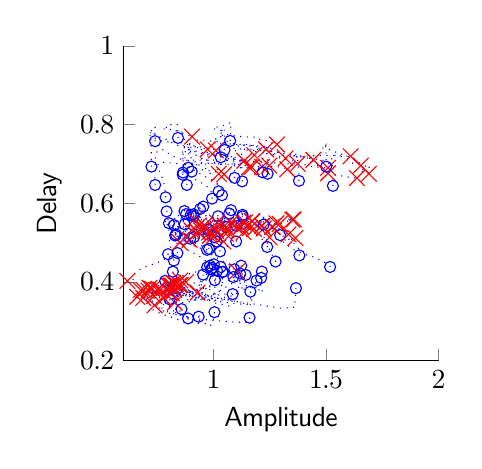
\begin{tikzpicture}

\begin{axis}[%
width=4cm,
height=4cm,
scale only axis,
xmin=0.6,
xmax=2,
xlabel={Amplitude},
ymin=0.2,
ymax=1,
ylabel={Delay},
axis x line*=bottom,
axis y line*=left
]
\addplot [
color=blue,
dotted,
forget plot
]
table[row sep=crcr]{
1.1911871338345 0.403754023531336\\
1.19107245246544 0.40286865394628\\
1.1902627766763 0.395550789042124\\
1.18427486439907 0.37164713666071\\
1.1640585290288 0.347444317036289\\
1.14719268781523 0.342373533610402\\
1.05669755489146 0.347863667798153\\
0.949785741549361 0.355643983589308\\
0.890630742293686 0.353630481853549\\
0.863444900162719 0.359895393735288\\
0.831881659060185 0.371097773229338\\
0.814803585421335 0.371843396217286\\
};
\addplot [
color=blue,
only marks,
mark=o,
mark options={solid},
forget plot
]
table[row sep=crcr]{
1.1911871338345 0.403754023531336\\
};
\addplot [
color=red,
mark size=4.0pt,
only marks,
mark=x,
mark options={solid},
forget plot
]
table[row sep=crcr]{
0.814803585421335 0.371843396217286\\
};
\addplot [
color=blue,
dotted,
forget plot
]
table[row sep=crcr]{
0.896579562917472 0.510093067916153\\
0.896671814794362 0.510651779333333\\
0.896761069379062 0.517222476634356\\
0.897522701851744 0.544198573882535\\
0.915170672960283 0.553015618836689\\
0.99064555099564 0.545713118206154\\
1.08395318741998 0.544944300298449\\
1.1291707406917 0.551242779870464\\
1.17059686248707 0.55459769428558\\
};
\addplot [
color=blue,
only marks,
mark=o,
mark options={solid},
forget plot
]
table[row sep=crcr]{
0.896579562917472 0.510093067916153\\
};
\addplot [
color=red,
mark size=4.0pt,
only marks,
mark=x,
mark options={solid},
forget plot
]
table[row sep=crcr]{
1.17059686248707 0.55459769428558\\
};
\addplot [
color=blue,
dotted,
forget plot
]
table[row sep=crcr]{
0.866318655613795 0.509196885495043\\
0.865963022277325 0.509829123618696\\
0.866447082769273 0.513620463375854\\
0.867213646452673 0.53166829612834\\
0.869634214527148 0.536228880746554\\
0.891568406544423 0.528890520772972\\
0.882680951063392 0.523854735000519\\
0.923228026777718 0.519387157004707\\
0.976219340322531 0.522893101027349\\
1.01114563244949 0.53013381476334\\
};
\addplot [
color=blue,
only marks,
mark=o,
mark options={solid},
forget plot
]
table[row sep=crcr]{
0.866318655613795 0.509196885495043\\
};
\addplot [
color=red,
mark size=4.0pt,
only marks,
mark=x,
mark options={solid},
forget plot
]
table[row sep=crcr]{
1.01114563244949 0.53013381476334\\
};
\addplot [
color=blue,
dotted,
forget plot
]
table[row sep=crcr]{
1.51804937657681 0.438317818639162\\
1.517883687449 0.438542127274937\\
1.51711901213195 0.440375694231265\\
1.50325075406161 0.447044095746721\\
1.45557738269861 0.461323786807181\\
1.38181643301225 0.475914030123686\\
1.34384818525228 0.485287035609794\\
1.32296924861243 0.498442458952488\\
1.3008802046176 0.503663473967177\\
1.32202192193987 0.507531682460813\\
1.36978376910161 0.51000325497818\\
1.36367043064105 0.511889345257198\\
};
\addplot [
color=blue,
only marks,
mark=o,
mark options={solid},
forget plot
]
table[row sep=crcr]{
1.51804937657681 0.438317818639162\\
};
\addplot [
color=red,
mark size=4.0pt,
only marks,
mark=x,
mark options={solid},
forget plot
]
table[row sep=crcr]{
1.36367043064105 0.511889345257198\\
};
\addplot [
color=blue,
dotted,
forget plot
]
table[row sep=crcr]{
0.877812780680645 0.572528355929342\\
0.877699497663813 0.572735528883903\\
0.877228411387723 0.573071933628411\\
0.873916217867072 0.570475765794631\\
0.863739647796738 0.551435498309326\\
0.821484703600237 0.536557465194755\\
0.838047913610864 0.536662560336968\\
0.913554100984919 0.537367699623068\\
0.914217557248 0.536568735643902\\
0.934913849111449 0.543439029394021\\
};
\addplot [
color=blue,
only marks,
mark=o,
mark options={solid},
forget plot
]
table[row sep=crcr]{
0.877812780680645 0.572528355929342\\
};
\addplot [
color=red,
mark size=4.0pt,
only marks,
mark=x,
mark options={solid},
forget plot
]
table[row sep=crcr]{
0.934913849111449 0.543439029394021\\
};
\addplot [
color=blue,
dotted,
forget plot
]
table[row sep=crcr]{
0.881187365129719 0.646628996328324\\
0.881264287322339 0.647254035132442\\
0.880291382283179 0.654726101259882\\
0.875884182887041 0.692501496689294\\
0.870954177493345 0.729992907374633\\
0.885609534813981 0.734500035776856\\
0.886057857646534 0.730315816034348\\
0.92199372528228 0.722302279106519\\
0.949403581965873 0.712370192967537\\
0.987921630248302 0.707578203430256\\
1.03570576671024 0.697541337763777\\
1.01746616591982 0.686578276947596\\
1.04683965017336 0.673515325959464\\
};
\addplot [
color=blue,
only marks,
mark=o,
mark options={solid},
forget plot
]
table[row sep=crcr]{
0.881187365129719 0.646628996328324\\
};
\addplot [
color=red,
mark size=4.0pt,
only marks,
mark=x,
mark options={solid},
forget plot
]
table[row sep=crcr]{
1.04683965017336 0.673515325959464\\
};
\addplot [
color=blue,
dotted,
forget plot
]
table[row sep=crcr]{
0.933760770950628 0.311982767819457\\
0.934026022661736 0.312148288351922\\
0.933428585344237 0.309872168788193\\
0.936488094762962 0.298536035480467\\
0.931007650008108 0.294213551273579\\
0.889508430039164 0.301599830914435\\
0.887025521674859 0.311754871048732\\
0.848310027842582 0.315284865640416\\
0.80864861909124 0.31978033506204\\
0.783862179968816 0.324300616642472\\
0.773485866298291 0.327300360328595\\
0.758614404570766 0.327849163986791\\
0.759460233683769 0.333412654469923\\
0.748687238389722 0.338976982918604\\
0.737839585872187 0.340814784167316\\
};
\addplot [
color=blue,
only marks,
mark=o,
mark options={solid},
forget plot
]
table[row sep=crcr]{
0.933760770950628 0.311982767819457\\
};
\addplot [
color=red,
mark size=4.0pt,
only marks,
mark=x,
mark options={solid},
forget plot
]
table[row sep=crcr]{
0.737839585872187 0.340814784167316\\
};
\addplot [
color=blue,
dotted,
forget plot
]
table[row sep=crcr]{
1.10033055958478 0.503095972319967\\
1.10053339540487 0.50341193014072\\
1.10148579593557 0.505097596279417\\
1.10238478909865 0.505408390887632\\
1.10245387042179 0.497890278425479\\
1.06272011002207 0.490859293273171\\
1.03932829169427 0.491016730782715\\
1.02727452309033 0.492214127174761\\
1.0201526601137 0.493224044119792\\
1.00270963583145 0.492561728150853\\
0.996107831077815 0.496753070552972\\
1.01545120145583 0.497672605192509\\
1.04468734395455 0.503362849727065\\
1.04378805990546 0.502993417003147\\
};
\addplot [
color=blue,
only marks,
mark=o,
mark options={solid},
forget plot
]
table[row sep=crcr]{
1.10033055958478 0.503095972319967\\
};
\addplot [
color=red,
mark size=4.0pt,
only marks,
mark=x,
mark options={solid},
forget plot
]
table[row sep=crcr]{
1.04378805990546 0.502993417003147\\
};
\addplot [
color=blue,
dotted,
forget plot
]
table[row sep=crcr]{
0.740030547688391 0.757732926553184\\
0.740087661854201 0.758532421538701\\
0.739728672747346 0.765971202601214\\
0.741358499584176 0.791281309423609\\
0.738239731403256 0.795260326183124\\
0.732949735276826 0.787924588220314\\
0.718498744025864 0.782833151049009\\
0.71230364853992 0.777483031955714\\
0.718394590972954 0.774933669325621\\
0.718287079689153 0.769866457921084\\
0.736026064231089 0.767791403333923\\
0.745783537700253 0.762583281125006\\
0.779999209962823 0.75612708024757\\
0.831209445259614 0.75665037142208\\
0.871938506316799 0.750845881834524\\
0.921021572617453 0.744822744517378\\
0.996699985039047 0.738939248427957\\
1.01042041691475 0.734264719418978\\
};
\addplot [
color=blue,
only marks,
mark=o,
mark options={solid},
forget plot
]
table[row sep=crcr]{
0.740030547688391 0.757732926553184\\
};
\addplot [
color=red,
mark size=4.0pt,
only marks,
mark=x,
mark options={solid},
forget plot
]
table[row sep=crcr]{
1.01042041691475 0.734264719418978\\
};
\addplot [
color=blue,
dotted,
forget plot
]
table[row sep=crcr]{
1.09220667705486 0.432233394252522\\
1.09181800218845 0.432440540326399\\
1.09095472957889 0.433450625094127\\
1.08360886972437 0.439391934863511\\
1.03582007081119 0.45477402668014\\
0.966538944907208 0.477780491533988\\
0.946437077446907 0.485041808116842\\
0.896531036094264 0.495327211095716\\
0.899744866117302 0.498991476671864\\
0.891458045833419 0.503115736722695\\
0.869955701188166 0.504492696357581\\
0.893685742127452 0.508328962918791\\
0.893132149571864 0.507363817965765\\
};
\addplot [
color=blue,
only marks,
mark=o,
mark options={solid},
forget plot
]
table[row sep=crcr]{
1.09220667705486 0.432233394252522\\
};
\addplot [
color=red,
mark size=4.0pt,
only marks,
mark=x,
mark options={solid},
forget plot
]
table[row sep=crcr]{
0.893132149571864 0.507363817965765\\
};
\addplot [
color=blue,
dotted,
forget plot
]
table[row sep=crcr]{
0.839439777412289 0.473598011817579\\
0.839564906701312 0.474181975763674\\
0.83912651298965 0.47796525726389\\
0.837768285953756 0.496861991153153\\
0.828939808668673 0.528879154409537\\
0.844189870111309 0.543409730838656\\
0.902149203900621 0.533515226374616\\
1.092655399312 0.532130744780873\\
1.17979290777024 0.534735289497099\\
};
\addplot [
color=blue,
only marks,
mark=o,
mark options={solid},
forget plot
]
table[row sep=crcr]{
0.839439777412289 0.473598011817579\\
};
\addplot [
color=red,
mark size=4.0pt,
only marks,
mark=x,
mark options={solid},
forget plot
]
table[row sep=crcr]{
1.17979290777024 0.534735289497099\\
};
\addplot [
color=blue,
dotted,
forget plot
]
table[row sep=crcr]{
1.00406712113522 0.323392800216983\\
1.00405896632684 0.322844809797328\\
1.00233955838598 0.319311689508415\\
0.998537684813798 0.299753133666016\\
0.984275609725462 0.288087362521468\\
0.935269344752395 0.302655052063797\\
0.887076799592621 0.307006234911141\\
0.882441039969186 0.311550882568222\\
0.864804277357277 0.317021242670775\\
0.829757610066497 0.321759179643404\\
0.840612412070787 0.32676666030351\\
0.855386216353731 0.335079019772556\\
0.847797777427665 0.338478140809584\\
0.831804168187411 0.344697172140719\\
0.827585762240093 0.347544376899585\\
};
\addplot [
color=blue,
only marks,
mark=o,
mark options={solid},
forget plot
]
table[row sep=crcr]{
1.00406712113522 0.323392800216983\\
};
\addplot [
color=red,
mark size=4.0pt,
only marks,
mark=x,
mark options={solid},
forget plot
]
table[row sep=crcr]{
0.827585762240093 0.347544376899585\\
};
\addplot [
color=blue,
dotted,
forget plot
]
table[row sep=crcr]{
1.1290098456739 0.566629086856372\\
1.12893288149519 0.566650317602662\\
1.12934827275923 0.568446694266619\\
1.12944824116236 0.566629615986681\\
1.12989077074562 0.550343079195833\\
1.12306170789873 0.536212891006355\\
1.15592514586325 0.529401949949402\\
1.16309407097099 0.532845693760539\\
1.1840701341637 0.535435624304054\\
1.22312825547255 0.536136592543838\\
};
\addplot [
color=blue,
only marks,
mark=o,
mark options={solid},
forget plot
]
table[row sep=crcr]{
1.1290098456739 0.566629086856372\\
};
\addplot [
color=red,
mark size=4.0pt,
only marks,
mark=x,
mark options={solid},
forget plot
]
table[row sep=crcr]{
1.22312825547255 0.536136592543838\\
};
\addplot [
color=blue,
dotted,
forget plot
]
table[row sep=crcr]{
1.0376500710662 0.620597013315194\\
1.03784770626483 0.621285969630006\\
1.03738335327881 0.627976593159755\\
1.03098825086456 0.645808564959667\\
0.994650188358967 0.658444226577468\\
0.945019494495369 0.673558009677483\\
0.913356253117159 0.683654360148081\\
0.916077171290191 0.693713068898562\\
0.927917711943757 0.700569476774027\\
0.89662379845487 0.702063687957432\\
0.912041748712519 0.70547146282257\\
0.919897855149524 0.705378132297274\\
0.967491401255994 0.702319206558486\\
0.973951467353638 0.701650001507679\\
1.0645940057753 0.69863585739724\\
1.08994098105317 0.697227102021628\\
1.09655523716009 0.692638276787887\\
1.11802495076991 0.690098147356677\\
1.15802503879966 0.691368427463415\\
};
\addplot [
color=blue,
only marks,
mark=o,
mark options={solid},
forget plot
]
table[row sep=crcr]{
1.0376500710662 0.620597013315194\\
};
\addplot [
color=red,
mark size=4.0pt,
only marks,
mark=x,
mark options={solid},
forget plot
]
table[row sep=crcr]{
1.15802503879966 0.691368427463415\\
};
\addplot [
color=blue,
dotted,
forget plot
]
table[row sep=crcr]{
0.95364242481725 0.418827492339648\\
0.953702617713166 0.418212112572406\\
0.954049886442296 0.413710546729832\\
0.945172016311794 0.392507260654016\\
0.932226263495347 0.369363466276133\\
0.915641255814678 0.361018095719495\\
0.921596835852128 0.356784740225591\\
0.932384712660245 0.360310992397952\\
0.886882787653677 0.376599825599339\\
0.880737979370007 0.38043348181199\\
0.873534403900191 0.383710485097942\\
0.852169302789162 0.403890908792821\\
};
\addplot [
color=blue,
only marks,
mark=o,
mark options={solid},
forget plot
]
table[row sep=crcr]{
0.95364242481725 0.418827492339648\\
};
\addplot [
color=red,
mark size=4.0pt,
only marks,
mark=x,
mark options={solid},
forget plot
]
table[row sep=crcr]{
0.852169302789162 0.403890908792821\\
};
\addplot [
color=blue,
dotted,
forget plot
]
table[row sep=crcr]{
0.993450961168605 0.611819312012629\\
0.993448740899786 0.612490323030181\\
0.992594367644577 0.618093482975431\\
0.986434698172063 0.635518434104058\\
0.952707657906683 0.649865713841211\\
0.889510094615634 0.669098837215566\\
0.884582440646117 0.680133793993543\\
0.901270189410617 0.691096416526552\\
0.915697777068798 0.697249565809953\\
0.932542491178466 0.69720007352808\\
0.982801727201515 0.700862215900445\\
1.10060648333345 0.699552018480277\\
1.16612168706204 0.694108214118763\\
1.26195380393863 0.692834924236075\\
1.29504089347104 0.692539775100557\\
1.31914665869751 0.688847562484336\\
1.32790786490157 0.686228831020794\\
};
\addplot [
color=blue,
only marks,
mark=o,
mark options={solid},
forget plot
]
table[row sep=crcr]{
0.993450961168605 0.611819312012629\\
};
\addplot [
color=red,
mark size=4.0pt,
only marks,
mark=x,
mark options={solid},
forget plot
]
table[row sep=crcr]{
1.32790786490157 0.686228831020794\\
};
\addplot [
color=blue,
dotted,
forget plot
]
table[row sep=crcr]{
1.36622474081335 0.384500600881149\\
1.36607651815887 0.383528914443824\\
1.36626339043565 0.374296686106718\\
1.36070177018423 0.346657651977424\\
1.36224466008856 0.3362631901371\\
1.30407422234018 0.333289880271136\\
1.0770420999944 0.352881155842927\\
0.982132652762614 0.363421443964738\\
0.927574805823863 0.372998464152289\\
0.92876257740946 0.373292482664005\\
};
\addplot [
color=blue,
only marks,
mark=o,
mark options={solid},
forget plot
]
table[row sep=crcr]{
1.36622474081335 0.384500600881149\\
};
\addplot [
color=red,
mark size=4.0pt,
only marks,
mark=x,
mark options={solid},
forget plot
]
table[row sep=crcr]{
0.92876257740946 0.373292482664005\\
};
\addplot [
color=blue,
dotted,
forget plot
]
table[row sep=crcr]{
1.37961281458799 0.657025686257541\\
1.37918170069694 0.65927876467749\\
1.37911953754503 0.677967904399541\\
1.37231845315455 0.719847684359436\\
1.35778409211499 0.72944286837626\\
1.35614687030252 0.721441114031616\\
1.43156549277472 0.713367464038328\\
1.44019382578056 0.704145089761768\\
1.47178911842427 0.6927475099944\\
1.52899659057687 0.673740496098347\\
1.60130974727062 0.666140733789807\\
1.63749795628765 0.664187387778492\\
};
\addplot [
color=blue,
only marks,
mark=o,
mark options={solid},
forget plot
]
table[row sep=crcr]{
1.37961281458799 0.657025686257541\\
};
\addplot [
color=red,
mark size=4.0pt,
only marks,
mark=x,
mark options={solid},
forget plot
]
table[row sep=crcr]{
1.63749795628765 0.664187387778492\\
};
\addplot [
color=blue,
dotted,
forget plot
]
table[row sep=crcr]{
0.898776177266458 0.570725951797528\\
0.8986608442657 0.570818844393165\\
0.899085965730904 0.570066571419393\\
0.896418874381662 0.566640614831168\\
0.889904199410379 0.551864642781893\\
0.900888875194638 0.539857245605357\\
0.978036189708013 0.544084496382552\\
0.976624323082939 0.534802000201914\\
0.96061221759744 0.532536187615554\\
1.00616865705245 0.535996802551157\\
};
\addplot [
color=blue,
only marks,
mark=o,
mark options={solid},
forget plot
]
table[row sep=crcr]{
0.898776177266458 0.570725951797528\\
};
\addplot [
color=red,
mark size=4.0pt,
only marks,
mark=x,
mark options={solid},
forget plot
]
table[row sep=crcr]{
1.00616865705245 0.535996802551157\\
};
\addplot [
color=blue,
dotted,
forget plot
]
table[row sep=crcr]{
1.09359936011185 0.664571440890097\\
1.0930362709148 0.666730557518129\\
1.09267017940295 0.681272547903155\\
1.09624092900806 0.721080563372298\\
1.09769541292845 0.743125005328229\\
1.12690472182547 0.748483874182828\\
1.21698749546994 0.744980601883371\\
1.31675239057896 0.731110750820391\\
1.3234245216356 0.71962131455809\\
1.4390626023199 0.720794444337661\\
1.50879642884301 0.721576217583061\\
1.60922228132455 0.719332130437785\\
};
\addplot [
color=blue,
only marks,
mark=o,
mark options={solid},
forget plot
]
table[row sep=crcr]{
1.09359936011185 0.664571440890097\\
};
\addplot [
color=red,
mark size=4.0pt,
only marks,
mark=x,
mark options={solid},
forget plot
]
table[row sep=crcr]{
1.60922228132455 0.719332130437785\\
};
\addplot [
color=blue,
dotted,
forget plot
]
table[row sep=crcr]{
0.740360975792337 0.64657191974317\\
0.740189309847223 0.647812020324357\\
0.739618932403256 0.655130577823378\\
0.738707377086341 0.690201344856533\\
0.743287440567729 0.728885515660888\\
0.77264974632247 0.736899792756664\\
0.787720597715214 0.730214958133292\\
0.823676736983271 0.718405933676084\\
0.868181646297933 0.709355768514127\\
0.956302067294485 0.709921980112518\\
1.08003236541819 0.709843589298232\\
1.1364252250213 0.708032063446114\\
};
\addplot [
color=blue,
only marks,
mark=o,
mark options={solid},
forget plot
]
table[row sep=crcr]{
0.740360975792337 0.64657191974317\\
};
\addplot [
color=red,
mark size=4.0pt,
only marks,
mark=x,
mark options={solid},
forget plot
]
table[row sep=crcr]{
1.1364252250213 0.708032063446114\\
};
\addplot [
color=blue,
dotted,
forget plot
]
table[row sep=crcr]{
0.723896849628153 0.693109955176957\\
0.723763568055095 0.694213235429688\\
0.723107040973845 0.702942099183051\\
0.722811848301973 0.744506410629898\\
0.719877596058377 0.78359018560941\\
0.72299621362058 0.78006056147499\\
0.733600751157035 0.776834297335621\\
0.748098863156438 0.772589664773085\\
0.766884142583412 0.766548160652526\\
0.796474871587151 0.760977013863479\\
0.809100823969171 0.755781888570407\\
0.832256579713283 0.748317011278892\\
0.889366201667775 0.742156513955555\\
0.950464385813338 0.741033214684437\\
0.973868357536927 0.737059896031331\\
};
\addplot [
color=blue,
only marks,
mark=o,
mark options={solid},
forget plot
]
table[row sep=crcr]{
0.723896849628153 0.693109955176957\\
};
\addplot [
color=red,
mark size=4.0pt,
only marks,
mark=x,
mark options={solid},
forget plot
]
table[row sep=crcr]{
0.973868357536927 0.737059896031331\\
};
\addplot [
color=blue,
dotted,
forget plot
]
table[row sep=crcr]{
1.27569786019753 0.451985860209872\\
1.27613921656206 0.452199324262655\\
1.27459079148766 0.453474552128059\\
1.26635073397919 0.462417174878675\\
1.24936742030586 0.481313905026686\\
1.23733786542052 0.502332466391676\\
1.20640778106729 0.511620693123507\\
1.23869059010935 0.514740340782077\\
1.24866824571241 0.513354759214194\\
};
\addplot [
color=blue,
only marks,
mark=o,
mark options={solid},
forget plot
]
table[row sep=crcr]{
1.27569786019753 0.451985860209872\\
};
\addplot [
color=red,
mark size=4.0pt,
only marks,
mark=x,
mark options={solid},
forget plot
]
table[row sep=crcr]{
1.24866824571241 0.513354759214194\\
};
\addplot [
color=blue,
dotted,
forget plot
]
table[row sep=crcr]{
1.0055112464817 0.513548102085562\\
1.00556448476 0.51445672553914\\
1.00396662987618 0.520686594111404\\
0.997561559852884 0.546010656649197\\
1.02023540576188 0.555979077483277\\
1.05471828537596 0.553633597270513\\
1.14109728156951 0.54004336829247\\
1.19999363929694 0.535577675997251\\
1.26023015100216 0.540225805384455\\
};
\addplot [
color=blue,
only marks,
mark=o,
mark options={solid},
forget plot
]
table[row sep=crcr]{
1.0055112464817 0.513548102085562\\
};
\addplot [
color=red,
mark size=4.0pt,
only marks,
mark=x,
mark options={solid},
forget plot
]
table[row sep=crcr]{
1.26023015100216 0.540225805384455\\
};
\addplot [
color=blue,
dotted,
forget plot
]
table[row sep=crcr]{
0.863159580046605 0.67266477107474\\
0.863165273203282 0.674194242984795\\
0.863590948992411 0.687875033738761\\
0.865292806635222 0.73276168090453\\
0.871334869162614 0.743278129282107\\
0.901344127857279 0.734524405794252\\
0.970496079966606 0.727215038832263\\
1.03779405402171 0.717533013254449\\
1.06766975051023 0.713041609433201\\
1.15052843125841 0.707385813283017\\
1.21645075870271 0.704855115606327\\
1.33458815993367 0.699811560078664\\
1.37373730052604 0.700285970172882\\
};
\addplot [
color=blue,
only marks,
mark=o,
mark options={solid},
forget plot
]
table[row sep=crcr]{
0.863159580046605 0.67266477107474\\
};
\addplot [
color=red,
mark size=4.0pt,
only marks,
mark=x,
mark options={solid},
forget plot
]
table[row sep=crcr]{
1.37373730052604 0.700285970172882\\
};
\addplot [
color=blue,
dotted,
forget plot
]
table[row sep=crcr]{
1.03942867934615 0.425247508842803\\
1.03894043754747 0.424726506556387\\
1.04018029164525 0.420820750646815\\
1.03310876386375 0.408385759222462\\
0.994229745019567 0.391633437986833\\
0.904434475584526 0.377895689146824\\
0.862255099738012 0.368885542578186\\
0.831222986997272 0.360259089053657\\
0.80428661802176 0.354911684104202\\
0.775025647581338 0.356298901751463\\
0.766697631327331 0.359465006841421\\
0.744932729332604 0.361255659977553\\
0.736971796340663 0.366150627608835\\
0.731462856934703 0.364973454201171\\
0.719693775699162 0.366677000188331\\
0.733354266269002 0.376869655103757\\
0.727877036517904 0.382710177448474\\
};
\addplot [
color=blue,
only marks,
mark=o,
mark options={solid},
forget plot
]
table[row sep=crcr]{
1.03942867934615 0.425247508842803\\
};
\addplot [
color=red,
mark size=4.0pt,
only marks,
mark=x,
mark options={solid},
forget plot
]
table[row sep=crcr]{
0.727877036517904 0.382710177448474\\
};
\addplot [
color=blue,
dotted,
forget plot
]
table[row sep=crcr]{
1.29584435319674 0.519191387532902\\
1.29568813047259 0.520022391645782\\
1.29576572320123 0.525422988957427\\
1.29293107660844 0.535281193163853\\
1.28742441648754 0.534075557679375\\
1.27426204229287 0.527971561705119\\
1.3230976063928 0.524412642631633\\
1.33307742356793 0.521032915092006\\
};
\addplot [
color=blue,
only marks,
mark=o,
mark options={solid},
forget plot
]
table[row sep=crcr]{
1.29584435319674 0.519191387532902\\
};
\addplot [
color=red,
mark size=4.0pt,
only marks,
mark=x,
mark options={solid},
forget plot
]
table[row sep=crcr]{
1.33307742356793 0.521032915092006\\
};
\addplot [
color=blue,
dotted,
forget plot
]
table[row sep=crcr]{
1.12712124934056 0.655633970129097\\
1.12736671452601 0.65709823912129\\
1.12715911167486 0.670754283807992\\
1.12537407926365 0.707770532000848\\
1.12454597327124 0.732536579731619\\
1.14024696143691 0.738332974172343\\
1.19149217281335 0.73701804440158\\
1.26909301709053 0.731381709931789\\
1.31988296874108 0.725752913953172\\
1.39007998245723 0.716455307336503\\
1.47937717047211 0.710275591297125\\
1.52336262193885 0.697376929579901\\
1.50894729184803 0.689909221984193\\
};
\addplot [
color=blue,
only marks,
mark=o,
mark options={solid},
forget plot
]
table[row sep=crcr]{
1.12712124934056 0.655633970129097\\
};
\addplot [
color=red,
mark size=4.0pt,
only marks,
mark=x,
mark options={solid},
forget plot
]
table[row sep=crcr]{
1.50894729184803 0.689909221984193\\
};
\addplot [
color=blue,
dotted,
forget plot
]
table[row sep=crcr]{
1.10190214514476 0.542405757597461\\
1.10186143338383 0.54273465900572\\
1.10034165826827 0.543298439090846\\
1.09823916342394 0.546051688608809\\
1.07629479996965 0.536540627136964\\
1.0468019108544 0.525158803965271\\
1.10220743270376 0.528053878727396\\
1.12716309850322 0.528671420654611\\
1.1334422699274 0.526457642710626\\
};
\addplot [
color=blue,
only marks,
mark=o,
mark options={solid},
forget plot
]
table[row sep=crcr]{
1.10190214514476 0.542405757597461\\
};
\addplot [
color=red,
mark size=4.0pt,
only marks,
mark=x,
mark options={solid},
forget plot
]
table[row sep=crcr]{
1.1334422699274 0.526457642710626\\
};
\addplot [
color=blue,
dotted,
forget plot
]
table[row sep=crcr]{
0.804717938335003 0.356197236479124\\
0.804705953245463 0.355584376161315\\
0.804643694761418 0.352563593013326\\
0.804356711181746 0.338089231429657\\
0.806577572405815 0.336072954599878\\
0.804409073489394 0.343652255234696\\
0.829263094740399 0.350212998024063\\
0.813903624362194 0.363711163036191\\
0.756946891851873 0.373678440776352\\
0.756175049240824 0.382450758596805\\
};
\addplot [
color=blue,
only marks,
mark=o,
mark options={solid},
forget plot
]
table[row sep=crcr]{
0.804717938335003 0.356197236479124\\
};
\addplot [
color=red,
mark size=4.0pt,
only marks,
mark=x,
mark options={solid},
forget plot
]
table[row sep=crcr]{
0.756175049240824 0.382450758596805\\
};
\addplot [
color=blue,
dotted,
forget plot
]
table[row sep=crcr]{
0.912027002319555 0.566398577482659\\
0.911767285278083 0.566706678177111\\
0.912950121444897 0.568846006768856\\
0.911847098884608 0.573101839799465\\
0.920541261537706 0.560726015226653\\
0.982902420722083 0.55442960050339\\
1.07256663717064 0.553762646199038\\
1.12487691410548 0.548081238706869\\
1.13210042559704 0.550972167770135\\
};
\addplot [
color=blue,
only marks,
mark=o,
mark options={solid},
forget plot
]
table[row sep=crcr]{
0.912027002319555 0.566398577482659\\
};
\addplot [
color=red,
mark size=4.0pt,
only marks,
mark=x,
mark options={solid},
forget plot
]
table[row sep=crcr]{
1.13210042559704 0.550972167770135\\
};
\addplot [
color=blue,
dotted,
forget plot
]
table[row sep=crcr]{
0.787024483276871 0.615170721880544\\
0.786951568348497 0.615383724136137\\
0.785961796900393 0.61854083385451\\
0.783582537918989 0.636076934641166\\
0.776696154385112 0.658872914534523\\
0.759628354102522 0.681883793977613\\
0.754123840576699 0.69855647207547\\
0.762430101971931 0.704706946232776\\
0.804867251889787 0.702689144309103\\
0.845999146794753 0.700729656806864\\
0.880970727040716 0.694753719256367\\
0.922122223505134 0.687891351314626\\
1.02583139117254 0.6785630210016\\
1.02334588555463 0.674706915897411\\
};
\addplot [
color=blue,
only marks,
mark=o,
mark options={solid},
forget plot
]
table[row sep=crcr]{
0.787024483276871 0.615170721880544\\
};
\addplot [
color=red,
mark size=4.0pt,
only marks,
mark=x,
mark options={solid},
forget plot
]
table[row sep=crcr]{
1.02334588555463 0.674706915897411\\
};
\addplot [
color=blue,
dotted,
forget plot
]
table[row sep=crcr]{
1.05607825755519 0.5396381488775\\
1.0557701991351 0.540225997261397\\
1.05578073139697 0.544806128896645\\
1.04774474017578 0.556510589917555\\
1.05061072286484 0.553610865127784\\
1.05911034515619 0.549419037397836\\
1.1593181569727 0.547692518688717\\
1.23465592189317 0.54651762814721\\
1.29372256804259 0.54762200906974\\
};
\addplot [
color=blue,
only marks,
mark=o,
mark options={solid},
forget plot
]
table[row sep=crcr]{
1.05607825755519 0.5396381488775\\
};
\addplot [
color=red,
mark size=4.0pt,
only marks,
mark=x,
mark options={solid},
forget plot
]
table[row sep=crcr]{
1.29372256804259 0.54762200906974\\
};
\addplot [
color=blue,
dotted,
forget plot
]
table[row sep=crcr]{
0.819087052506453 0.426401396248375\\
0.818881425675953 0.425995294742254\\
0.818300141202713 0.422917119414901\\
0.816211703927032 0.401465231187238\\
0.811677248865177 0.369697584545003\\
0.820786656333993 0.355071446287603\\
0.806325389839192 0.358264690801236\\
0.784131327993265 0.37118415237723\\
0.763724216254892 0.373549254334254\\
0.733287560354163 0.381409348663536\\
0.715539661019554 0.385381661970277\\
};
\addplot [
color=blue,
only marks,
mark=o,
mark options={solid},
forget plot
]
table[row sep=crcr]{
0.819087052506453 0.426401396248375\\
};
\addplot [
color=red,
mark size=4.0pt,
only marks,
mark=x,
mark options={solid},
forget plot
]
table[row sep=crcr]{
0.715539661019554 0.385381661970277\\
};
\addplot [
color=blue,
dotted,
forget plot
]
table[row sep=crcr]{
1.24024333484124 0.674955506299082\\
1.24054019262012 0.677049704532085\\
1.24174990058734 0.692766983068046\\
1.23762153861503 0.733048527044665\\
1.23424553897129 0.735350906077908\\
1.27052803070767 0.72747071741771\\
1.27995208389264 0.717260588258652\\
1.33093074893846 0.709810173433924\\
1.37707474278672 0.704690979688518\\
1.42133739570656 0.694425694557597\\
1.51758704024249 0.689039117268283\\
1.51812903839097 0.681388582361573\\
1.50869683795744 0.676216614685812\\
};
\addplot [
color=blue,
only marks,
mark=o,
mark options={solid},
forget plot
]
table[row sep=crcr]{
1.24024333484124 0.674955506299082\\
};
\addplot [
color=red,
mark size=4.0pt,
only marks,
mark=x,
mark options={solid},
forget plot
]
table[row sep=crcr]{
1.50869683795744 0.676216614685812\\
};
\addplot [
color=blue,
dotted,
forget plot
]
table[row sep=crcr]{
0.970888278909198 0.481665332166258\\
0.970513623564114 0.481711180961798\\
0.970154496320668 0.482439503198796\\
0.967250683277513 0.48706821267636\\
0.908725371686447 0.501182513098697\\
0.819944256701437 0.520339012490328\\
0.810694755494564 0.535030663978309\\
0.80358658350412 0.546616447132083\\
0.778524928378594 0.55706183503881\\
0.806635060910585 0.558860764706158\\
0.835545079314947 0.562290988686019\\
0.846008530066843 0.562167723450102\\
0.856733509673008 0.560402329997672\\
0.873793263711807 0.562060501280193\\
0.90527797832384 0.563987846210314\\
0.917152616172489 0.561456607725086\\
0.91495971726863 0.559628675078279\\
};
\addplot [
color=blue,
only marks,
mark=o,
mark options={solid},
forget plot
]
table[row sep=crcr]{
0.970888278909198 0.481665332166258\\
};
\addplot [
color=red,
mark size=4.0pt,
only marks,
mark=x,
mark options={solid},
forget plot
]
table[row sep=crcr]{
0.91495971726863 0.559628675078279\\
};
\addplot [
color=blue,
dotted,
forget plot
]
table[row sep=crcr]{
1.38147176861864 0.467535123533309\\
1.380815822817 0.46812351033637\\
1.37982655595652 0.472169097324598\\
1.37720352787866 0.485986010173407\\
1.34915963731188 0.50372548059251\\
1.30336443682073 0.518464727859854\\
1.33553326755159 0.524107490494549\\
1.2925471984631 0.534812500394854\\
1.29012285596937 0.535383136490857\\
1.23178956087627 0.538055098861705\\
1.25097143490333 0.538937369771836\\
1.26253348615446 0.540385002268208\\
};
\addplot [
color=blue,
only marks,
mark=o,
mark options={solid},
forget plot
]
table[row sep=crcr]{
1.38147176861864 0.467535123533309\\
};
\addplot [
color=red,
mark size=4.0pt,
only marks,
mark=x,
mark options={solid},
forget plot
]
table[row sep=crcr]{
1.26253348615446 0.540385002268208\\
};
\addplot [
color=blue,
dotted,
forget plot
]
table[row sep=crcr]{
0.979940693485314 0.484286407253389\\
0.979531599472381 0.485211326577491\\
0.978834461046115 0.491053236678147\\
0.977905365325107 0.513217986150717\\
0.984029892381415 0.532013608594586\\
1.02582071497447 0.540547333059399\\
1.0909683062361 0.545270313039077\\
1.10071871678101 0.551748267770754\\
1.14062174059059 0.551188568001779\\
};
\addplot [
color=blue,
only marks,
mark=o,
mark options={solid},
forget plot
]
table[row sep=crcr]{
0.979940693485314 0.484286407253389\\
};
\addplot [
color=red,
mark size=4.0pt,
only marks,
mark=x,
mark options={solid},
forget plot
]
table[row sep=crcr]{
1.14062174059059 0.551188568001779\\
};
\addplot [
color=blue,
dotted,
forget plot
]
table[row sep=crcr]{
1.12862049070271 0.57066334757889\\
1.12879494362779 0.571073046049079\\
1.12740055813888 0.573313529066527\\
1.12932177740894 0.572198029852499\\
1.11514527174645 0.561131946069828\\
1.10365079661743 0.547770107065386\\
1.0689291770968 0.544923564053734\\
1.07073706090363 0.543755645086389\\
1.0816804750264 0.540830630130946\\
1.15986563764332 0.538883149133015\\
1.16317831666184 0.537511217162765\\
};
\addplot [
color=blue,
only marks,
mark=o,
mark options={solid},
forget plot
]
table[row sep=crcr]{
1.12862049070271 0.57066334757889\\
};
\addplot [
color=red,
mark size=4.0pt,
only marks,
mark=x,
mark options={solid},
forget plot
]
table[row sep=crcr]{
1.16317831666184 0.537511217162765\\
};
\addplot [
color=blue,
dotted,
forget plot
]
table[row sep=crcr]{
1.0226516613127 0.63036156742075\\
1.02233996298286 0.631217917793451\\
1.02106548468453 0.637094595689342\\
1.01332741842715 0.655830002736429\\
0.987689681533731 0.674693630746908\\
0.951489297530248 0.695135836133294\\
0.938235274806579 0.708673184658243\\
0.954274588675282 0.717701489149389\\
0.997280098531735 0.722835379426031\\
1.027800337646 0.722696664300794\\
1.08555338430165 0.719873819481333\\
1.07056827284549 0.716703094835559\\
1.09709422215574 0.713237103109662\\
1.13075921508383 0.707974298475097\\
1.1815956020007 0.705922294121838\\
1.20598157994535 0.701013100234104\\
1.2475930592193 0.695751591991471\\
};
\addplot [
color=blue,
only marks,
mark=o,
mark options={solid},
forget plot
]
table[row sep=crcr]{
1.0226516613127 0.63036156742075\\
};
\addplot [
color=red,
mark size=4.0pt,
only marks,
mark=x,
mark options={solid},
forget plot
]
table[row sep=crcr]{
1.2475930592193 0.695751591991471\\
};
\addplot [
color=blue,
dotted,
forget plot
]
table[row sep=crcr]{
1.53056917360816 0.644235818736112\\
1.53090712817296 0.647194290771188\\
1.53084748662895 0.666621920307052\\
1.5270953628503 0.703841289727506\\
1.52396694867216 0.720644878053931\\
1.53764482736644 0.721977043487062\\
1.59229489677654 0.715260276805904\\
1.6214929111811 0.700365589016275\\
1.69793582084237 0.692318222004348\\
1.64829667693148 0.68244538847962\\
1.69030964466257 0.67488551569363\\
};
\addplot [
color=blue,
only marks,
mark=o,
mark options={solid},
forget plot
]
table[row sep=crcr]{
1.53056917360816 0.644235818736112\\
};
\addplot [
color=red,
mark size=4.0pt,
only marks,
mark=x,
mark options={solid},
forget plot
]
table[row sep=crcr]{
1.69030964466257 0.67488551569363\\
};
\addplot [
color=blue,
dotted,
forget plot
]
table[row sep=crcr]{
0.913519806356853 0.514123421882024\\
0.913542880874851 0.514889460550131\\
0.912643558360566 0.520917043759923\\
0.911433231099072 0.545156317642788\\
0.916235760819384 0.559040766313327\\
0.96242683758921 0.557752066339914\\
1.00126940450538 0.552765546449253\\
1.02319625539556 0.544876513796569\\
1.04912385078252 0.543255511292474\\
};
\addplot [
color=blue,
only marks,
mark=o,
mark options={solid},
forget plot
]
table[row sep=crcr]{
0.913519806356853 0.514123421882024\\
};
\addplot [
color=red,
mark size=4.0pt,
only marks,
mark=x,
mark options={solid},
forget plot
]
table[row sep=crcr]{
1.04912385078252 0.543255511292474\\
};
\addplot [
color=blue,
dotted,
forget plot
]
table[row sep=crcr]{
0.87176815491695 0.546565963915279\\
0.871492216838302 0.547157828248667\\
0.870880599782471 0.551692163886542\\
0.870999273937521 0.57261825021661\\
0.875120941844731 0.575395263452122\\
0.911811797801658 0.567425614459643\\
0.957978380056279 0.562036100713293\\
0.992191333231532 0.555664095438031\\
1.03317434524149 0.557913848916678\\
1.03412970368316 0.552449617984018\\
1.07679441892463 0.550564119222713\\
};
\addplot [
color=blue,
only marks,
mark=o,
mark options={solid},
forget plot
]
table[row sep=crcr]{
0.87176815491695 0.546565963915279\\
};
\addplot [
color=red,
mark size=4.0pt,
only marks,
mark=x,
mark options={solid},
forget plot
]
table[row sep=crcr]{
1.07679441892463 0.550564119222713\\
};
\addplot [
color=blue,
dotted,
forget plot
]
table[row sep=crcr]{
0.887787035582818 0.690278988150159\\
0.887992694580264 0.691185847655915\\
0.888511345234493 0.702501224376402\\
0.887735680966458 0.742757555956833\\
0.890246075284869 0.746952395034534\\
0.886546276628832 0.736615927705665\\
0.929508576282533 0.728566171938025\\
0.993552883067051 0.722331136509806\\
1.06139521310657 0.71891835309393\\
1.07836764391059 0.715088458382941\\
1.09500480580859 0.709977355289792\\
1.13714943835408 0.704867325760047\\
1.15465368295191 0.695548487998141\\
1.18378443554265 0.692471204081404\\
1.21506238574407 0.692443313323373\\
};
\addplot [
color=blue,
only marks,
mark=o,
mark options={solid},
forget plot
]
table[row sep=crcr]{
0.887787035582818 0.690278988150159\\
};
\addplot [
color=red,
mark size=4.0pt,
only marks,
mark=x,
mark options={solid},
forget plot
]
table[row sep=crcr]{
1.21506238574407 0.692443313323373\\
};
\addplot [
color=blue,
dotted,
forget plot
]
table[row sep=crcr]{
0.886799126839566 0.30747589644305\\
0.886441622620523 0.30745116036194\\
0.886347028800487 0.305850506982625\\
0.88245292406762 0.297704223871889\\
0.860473657962229 0.299870285698199\\
0.822931401752138 0.309194244192053\\
0.777894866040912 0.316881373828482\\
0.746939112247864 0.324349382057089\\
0.728316023594633 0.329871155091088\\
0.730821324011466 0.334869296723448\\
0.736419195685659 0.336029299139712\\
0.733718372743815 0.338090028164296\\
0.731338040652279 0.342717298966573\\
0.722246017726976 0.346263813258663\\
0.693104546303437 0.353558506547244\\
0.696019313954705 0.363510805808428\\
0.684580743154955 0.373941689838787\\
0.688228669491897 0.380077395350781\\
};
\addplot [
color=blue,
only marks,
mark=o,
mark options={solid},
forget plot
]
table[row sep=crcr]{
0.886799126839566 0.30747589644305\\
};
\addplot [
color=red,
mark size=4.0pt,
only marks,
mark=x,
mark options={solid},
forget plot
]
table[row sep=crcr]{
0.688228669491897 0.380077395350781\\
};
\addplot [
color=blue,
dotted,
forget plot
]
table[row sep=crcr]{
0.954228439767421 0.591555353218202\\
0.95415184957375 0.592074427117988\\
0.953601690576605 0.594153550083335\\
0.958282228304022 0.595055107520558\\
0.952195654503776 0.580168459497479\\
0.964396831351716 0.568821537928728\\
1.0015039434197 0.563177680084011\\
1.07261542132875 0.550547450853507\\
1.12932801230205 0.551899477302418\\
1.17279889999961 0.554235031841191\\
};
\addplot [
color=blue,
only marks,
mark=o,
mark options={solid},
forget plot
]
table[row sep=crcr]{
0.954228439767421 0.591555353218202\\
};
\addplot [
color=red,
mark size=4.0pt,
only marks,
mark=x,
mark options={solid},
forget plot
]
table[row sep=crcr]{
1.17279889999961 0.554235031841191\\
};
\addplot [
color=blue,
dotted,
forget plot
]
table[row sep=crcr]{
1.07762290461682 0.582531936140443\\
1.07738147476944 0.58268333140667\\
1.07804818574463 0.585049509860445\\
1.07276845922701 0.586013541399307\\
1.06064893392186 0.569769751286467\\
1.04423952099574 0.557983427003535\\
1.0558109812724 0.554011875095346\\
1.02834087357419 0.542604105237433\\
1.05776832382288 0.53298063173822\\
1.05725714117408 0.530765537138676\\
};
\addplot [
color=blue,
only marks,
mark=o,
mark options={solid},
forget plot
]
table[row sep=crcr]{
1.07762290461682 0.582531936140443\\
};
\addplot [
color=red,
mark size=4.0pt,
only marks,
mark=x,
mark options={solid},
forget plot
]
table[row sep=crcr]{
1.05725714117408 0.530765537138676\\
};
\addplot [
color=blue,
dotted,
forget plot
]
table[row sep=crcr]{
1.16001053525779 0.309482029613916\\
1.15983007079626 0.309291417017096\\
1.16093940349498 0.306905734936099\\
1.15530436094235 0.297818661452067\\
1.10605323448037 0.297683344055864\\
0.99625991249694 0.302603516792318\\
0.927332722472968 0.306489383246412\\
0.863508354781689 0.314488705857441\\
0.801561160328169 0.322346234566381\\
0.7717311711692 0.333488150947563\\
0.735779035912635 0.340334791868373\\
0.735542269104857 0.347294557513509\\
0.725279877681959 0.353710301450695\\
0.693441955614966 0.35724319233207\\
0.687134609512768 0.359719592598425\\
};
\addplot [
color=blue,
only marks,
mark=o,
mark options={solid},
forget plot
]
table[row sep=crcr]{
1.16001053525779 0.309482029613916\\
};
\addplot [
color=red,
mark size=4.0pt,
only marks,
mark=x,
mark options={solid},
forget plot
]
table[row sep=crcr]{
0.687134609512768 0.359719592598425\\
};
\addplot [
color=blue,
dotted,
forget plot
]
table[row sep=crcr]{
0.837565827372098 0.383358810408082\\
0.837694513984967 0.38291715084049\\
0.836883881937388 0.378565017641882\\
0.836034893056796 0.353184611958776\\
0.829009125792801 0.32173632095105\\
0.827308249110736 0.324850492437501\\
0.812416650601106 0.330281731337351\\
0.81103114587357 0.336374128584308\\
0.799316929034807 0.33274318366447\\
0.811791339084721 0.331457399669507\\
0.79466352797221 0.342563304445051\\
0.797948027343471 0.348407437823047\\
0.766971182907244 0.354988532608593\\
0.778300267226122 0.359538313025598\\
};
\addplot [
color=blue,
only marks,
mark=o,
mark options={solid},
forget plot
]
table[row sep=crcr]{
0.837565827372098 0.383358810408082\\
};
\addplot [
color=red,
mark size=4.0pt,
only marks,
mark=x,
mark options={solid},
forget plot
]
table[row sep=crcr]{
0.778300267226122 0.359538313025598\\
};
\addplot [
color=blue,
dotted,
forget plot
]
table[row sep=crcr]{
1.14264656837639 0.418075522242115\\
1.1427444826567 0.417287111180128\\
1.1420631525406 0.412251262692029\\
1.13577719659912 0.392962743449739\\
1.10675653336835 0.36795366249351\\
1.1001128522603 0.356839678613647\\
1.03048531869998 0.353616656381165\\
0.992111946318076 0.353965035427632\\
0.946903573851081 0.360556798633618\\
0.909749859497427 0.361044814756725\\
0.892157251615914 0.363689892327134\\
0.849998674445065 0.367815683974386\\
0.836395253837059 0.371582281296405\\
0.817621973164707 0.38972884852111\\
};
\addplot [
color=blue,
only marks,
mark=o,
mark options={solid},
forget plot
]
table[row sep=crcr]{
1.14264656837639 0.418075522242115\\
};
\addplot [
color=red,
mark size=4.0pt,
only marks,
mark=x,
mark options={solid},
forget plot
]
table[row sep=crcr]{
0.817621973164707 0.38972884852111\\
};
\addplot [
color=blue,
dotted,
forget plot
]
table[row sep=crcr]{
1.00577303460186 0.404586472028476\\
1.00565467459512 0.403799954664916\\
1.00456648757539 0.397468633198596\\
1.0072559759363 0.3715691875854\\
1.00096286126055 0.356768872845629\\
0.964096568257559 0.362024000678936\\
0.91287563876378 0.3696703461065\\
0.841128573602728 0.38233465683482\\
0.814367633156942 0.389033221035531\\
0.80768192295776 0.391098489503479\\
};
\addplot [
color=blue,
only marks,
mark=o,
mark options={solid},
forget plot
]
table[row sep=crcr]{
1.00577303460186 0.404586472028476\\
};
\addplot [
color=red,
mark size=4.0pt,
only marks,
mark=x,
mark options={solid},
forget plot
]
table[row sep=crcr]{
0.80768192295776 0.391098489503479\\
};
\addplot [
color=blue,
dotted,
forget plot
]
table[row sep=crcr]{
0.83282755593893 0.520779292494457\\
0.832528196605584 0.520908301573784\\
0.832705546165044 0.524495663700729\\
0.833091207135968 0.534337827828636\\
0.834510791253121 0.53310550988578\\
0.829189484941116 0.53113261247753\\
0.853187879416389 0.523565388977796\\
0.873415903189582 0.535729422947738\\
0.945303555178544 0.530514151123683\\
};
\addplot [
color=blue,
only marks,
mark=o,
mark options={solid},
forget plot
]
table[row sep=crcr]{
0.83282755593893 0.520779292494457\\
};
\addplot [
color=red,
mark size=4.0pt,
only marks,
mark=x,
mark options={solid},
forget plot
]
table[row sep=crcr]{
0.945303555178544 0.530514151123683\\
};
\addplot [
color=blue,
dotted,
forget plot
]
table[row sep=crcr]{
0.984132876034391 0.44164984326681\\
0.98401326144655 0.441815731327504\\
0.982220487616218 0.442635436027089\\
0.975676257905494 0.449380196765457\\
0.929230886554941 0.468798380604254\\
0.870197237313835 0.484925317935218\\
0.834289893107697 0.499935686820382\\
0.852463249834408 0.511472935807869\\
0.912767259831527 0.510573759715534\\
0.921891515244241 0.506686860650516\\
0.875107366441798 0.503783820067902\\
0.874629812237395 0.499436477993572\\
0.850147985977758 0.500435046868241\\
};
\addplot [
color=blue,
only marks,
mark=o,
mark options={solid},
forget plot
]
table[row sep=crcr]{
0.984132876034391 0.44164984326681\\
};
\addplot [
color=red,
mark size=4.0pt,
only marks,
mark=x,
mark options={solid},
forget plot
]
table[row sep=crcr]{
0.850147985977758 0.500435046868241\\
};
\addplot [
color=blue,
dotted,
forget plot
]
table[row sep=crcr]{
1.50055012858136 0.693028082873172\\
1.5005278849339 0.696289518341333\\
1.49988223449873 0.71687534953612\\
1.49886903154383 0.746068077109047\\
1.49718198507044 0.743794782229145\\
1.48053487768513 0.740835562736624\\
1.51662167620689 0.73685343986598\\
1.53925721819381 0.730728709961772\\
1.58588583000236 0.72179557706714\\
1.62199457788419 0.713154463948453\\
1.65028393200188 0.702384561947632\\
1.65220201942571 0.695715156126905\\
1.65468904108851 0.695827139489885\\
};
\addplot [
color=blue,
only marks,
mark=o,
mark options={solid},
forget plot
]
table[row sep=crcr]{
1.50055012858136 0.693028082873172\\
};
\addplot [
color=red,
mark size=4.0pt,
only marks,
mark=x,
mark options={solid},
forget plot
]
table[row sep=crcr]{
1.65468904108851 0.695827139489885\\
};
\addplot [
color=blue,
dotted,
forget plot
]
table[row sep=crcr]{
1.21148472409982 0.41043929827887\\
1.21128825587723 0.409699036107786\\
1.21131352879104 0.402194771841129\\
1.20948357594608 0.379564181944712\\
1.22283527075064 0.376076273150228\\
1.14886214776663 0.390000426630623\\
1.09219292690886 0.403108360493369\\
1.11560337267805 0.412790292487674\\
1.13566471026066 0.417691896842714\\
1.11582653795937 0.424083735267224\\
1.09733460837258 0.427693414523737\\
1.09211402454897 0.428111648622153\\
1.10452797850283 0.427412350812682\\
};
\addplot [
color=blue,
only marks,
mark=o,
mark options={solid},
forget plot
]
table[row sep=crcr]{
1.21148472409982 0.41043929827887\\
};
\addplot [
color=red,
mark size=4.0pt,
only marks,
mark=x,
mark options={solid},
forget plot
]
table[row sep=crcr]{
1.10452797850283 0.427412350812682\\
};
\addplot [
color=blue,
dotted,
forget plot
]
table[row sep=crcr]{
1.21803223533194 0.678739613887325\\
1.21763522604925 0.681484744001395\\
1.21747878925618 0.701252104046069\\
1.22315884345696 0.740706422969683\\
1.23586373369544 0.740999075069201\\
1.21968844047233 0.73493104843431\\
1.29969271804956 0.728450583351112\\
1.3053714284729 0.722877332732387\\
1.35765123643834 0.717462063544572\\
1.3985013318221 0.718110426144447\\
1.44312391254114 0.713506322369523\\
1.44369635286423 0.710237432465619\\
};
\addplot [
color=blue,
only marks,
mark=o,
mark options={solid},
forget plot
]
table[row sep=crcr]{
1.21803223533194 0.678739613887325\\
};
\addplot [
color=red,
mark size=4.0pt,
only marks,
mark=x,
mark options={solid},
forget plot
]
table[row sep=crcr]{
1.44369635286423 0.710237432465619\\
};
\addplot [
color=blue,
dotted,
forget plot
]
table[row sep=crcr]{
1.07402968121383 0.758461168035877\\
1.07441846331515 0.759952544210216\\
1.07526585167189 0.77395333302693\\
1.07756428776243 0.80616303265674\\
1.07710131201082 0.805380149361892\\
1.05324453497069 0.798919120880791\\
1.02116555951493 0.794699259045298\\
0.995830884501763 0.789878278084646\\
1.03406940193606 0.785287860008251\\
1.02111862487656 0.782416322969886\\
1.04239869474401 0.775923995129718\\
1.11267083340881 0.770340965573965\\
1.12876582836541 0.768912391565787\\
1.19610115869206 0.767767749199629\\
1.20679004813147 0.761720998569433\\
1.25045763159481 0.758535067153848\\
1.25801621188201 0.752767074391926\\
1.28189429577618 0.749392207617545\\
};
\addplot [
color=blue,
only marks,
mark=o,
mark options={solid},
forget plot
]
table[row sep=crcr]{
1.07402968121383 0.758461168035877\\
};
\addplot [
color=red,
mark size=4.0pt,
only marks,
mark=x,
mark options={solid},
forget plot
]
table[row sep=crcr]{
1.28189429577618 0.749392207617545\\
};
\addplot [
color=blue,
dotted,
forget plot
]
table[row sep=crcr]{
0.976628185625384 0.533362763129837\\
0.976606109491956 0.53446625350562\\
0.977619526099907 0.539128297841784\\
0.982734844592634 0.548203947081948\\
0.999823518499292 0.543052368096897\\
1.0491830679923 0.538700961787456\\
1.11288692612711 0.540355250321373\\
1.12200620904201 0.54108706165737\\
};
\addplot [
color=blue,
only marks,
mark=o,
mark options={solid},
forget plot
]
table[row sep=crcr]{
0.976628185625384 0.533362763129837\\
};
\addplot [
color=red,
mark size=4.0pt,
only marks,
mark=x,
mark options={solid},
forget plot
]
table[row sep=crcr]{
1.12200620904201 0.54108706165737\\
};
\addplot [
color=blue,
dotted,
forget plot
]
table[row sep=crcr]{
1.00104844291004 0.444963980606724\\
1.0013021916611 0.44501632641315\\
1.00027395927761 0.444013352428209\\
0.993625016174612 0.437700341281577\\
0.931004125549511 0.426966490182736\\
0.809270596901955 0.408192945551816\\
0.760552338218355 0.392868325374172\\
0.72425243395935 0.378562802211096\\
0.694154018052147 0.374397309503256\\
0.700301885197507 0.376558601003696\\
0.676632808455963 0.379399191317693\\
};
\addplot [
color=blue,
only marks,
mark=o,
mark options={solid},
forget plot
]
table[row sep=crcr]{
1.00104844291004 0.444963980606724\\
};
\addplot [
color=red,
mark size=4.0pt,
only marks,
mark=x,
mark options={solid},
forget plot
]
table[row sep=crcr]{
0.676632808455963 0.379399191317693\\
};
\addplot [
color=blue,
dotted,
forget plot
]
table[row sep=crcr]{
1.12292912179462 0.441599168440434\\
1.12299548955762 0.441256841905445\\
1.12188895597883 0.437166616000405\\
1.11438034653694 0.42446778119291\\
1.07865669176623 0.406091098005501\\
0.986695518522848 0.388713590451974\\
0.90453027720134 0.375589854279551\\
0.865795046116319 0.370440672122221\\
0.832318021845187 0.365075978695659\\
0.823389574183576 0.363882445611896\\
0.820144723201284 0.365212656691206\\
0.790232943206605 0.369768533006774\\
0.769903278717774 0.370389369789265\\
0.702847820497609 0.3746953148234\\
0.710921059098809 0.378015910147939\\
};
\addplot [
color=blue,
only marks,
mark=o,
mark options={solid},
forget plot
]
table[row sep=crcr]{
1.12292912179462 0.441599168440434\\
};
\addplot [
color=red,
mark size=4.0pt,
only marks,
mark=x,
mark options={solid},
forget plot
]
table[row sep=crcr]{
0.710921059098809 0.378015910147939\\
};
\addplot [
color=blue,
dotted,
forget plot
]
table[row sep=crcr]{
0.988607264988814 0.432481310751483\\
0.988170209653149 0.432155412826591\\
0.988261628857162 0.427491905752119\\
0.987086248082066 0.403443814408068\\
0.982763328902073 0.376686927549287\\
0.960616282364247 0.367225141940513\\
0.950862722788796 0.370721716207648\\
0.925090278630892 0.371932462616457\\
0.903934292244755 0.373804047751678\\
0.852522148746624 0.378263440402092\\
0.823848615985044 0.379791797809047\\
0.853511938631751 0.392538503702252\\
};
\addplot [
color=blue,
only marks,
mark=o,
mark options={solid},
forget plot
]
table[row sep=crcr]{
0.988607264988814 0.432481310751483\\
};
\addplot [
color=red,
mark size=4.0pt,
only marks,
mark=x,
mark options={solid},
forget plot
]
table[row sep=crcr]{
0.853511938631751 0.392538503702252\\
};
\addplot [
color=blue,
dotted,
forget plot
]
table[row sep=crcr]{
1.0847379338384 0.369285244973485\\
1.08468956674082 0.368526674101507\\
1.08568400023309 0.363133804906863\\
1.07902562866131 0.342352744139641\\
1.07029220806587 0.338942313414558\\
1.01104147724675 0.345949575710275\\
0.987066276509222 0.352253000867311\\
0.940069377807028 0.357562442412911\\
0.830829186362005 0.378049795860551\\
0.804064948686568 0.385615846740086\\
0.800471931006161 0.390847555487673\\
};
\addplot [
color=blue,
only marks,
mark=o,
mark options={solid},
forget plot
]
table[row sep=crcr]{
1.0847379338384 0.369285244973485\\
};
\addplot [
color=red,
mark size=4.0pt,
only marks,
mark=x,
mark options={solid},
forget plot
]
table[row sep=crcr]{
0.800471931006161 0.390847555487673\\
};
\addplot [
color=blue,
dotted,
forget plot
]
table[row sep=crcr]{
1.01362736165569 0.502630305849722\\
1.01343191412169 0.503113548460204\\
1.01455457315545 0.508480643838003\\
1.00753150543031 0.535270399762588\\
0.979634526975038 0.56153126690498\\
1.00750847219909 0.557118971770279\\
1.09838294426916 0.548313374677921\\
1.1325563676296 0.55204907281132\\
1.18965470278808 0.553931782469586\\
1.23571593514199 0.552107213113065\\
1.27968676492296 0.549178567231516\\
};
\addplot [
color=blue,
only marks,
mark=o,
mark options={solid},
forget plot
]
table[row sep=crcr]{
1.01362736165569 0.502630305849722\\
};
\addplot [
color=red,
mark size=4.0pt,
only marks,
mark=x,
mark options={solid},
forget plot
]
table[row sep=crcr]{
1.27968676492296 0.549178567231516\\
};
\addplot [
color=blue,
dotted,
forget plot
]
table[row sep=crcr]{
0.841861663662618 0.76599521244171\\
0.84196093073898 0.766973805362488\\
0.840949997489911 0.773890564888517\\
0.841812981801182 0.799221550868689\\
0.823926118955048 0.802422921141418\\
0.810802296519426 0.799885812649975\\
0.791335669191959 0.794592724937624\\
0.794326445387302 0.793164186952313\\
0.771021101068354 0.78924494039927\\
0.787220374045957 0.789035109282534\\
0.787202450527303 0.787984180429427\\
0.788000769694278 0.78826758236557\\
0.792252220974598 0.787473655993899\\
0.830121913080493 0.787332151053156\\
0.834967410694615 0.78342914545896\\
0.834103984973561 0.78169480455945\\
0.864712496688764 0.781215492379235\\
0.855817264430245 0.779642046556143\\
0.852660332392749 0.780424604089568\\
0.869093758904414 0.776016558797463\\
0.894302702431733 0.771892766093552\\
0.904469881527201 0.769405037467741\\
};
\addplot [
color=blue,
only marks,
mark=o,
mark options={solid},
forget plot
]
table[row sep=crcr]{
0.841861663662618 0.76599521244171\\
};
\addplot [
color=red,
mark size=4.0pt,
only marks,
mark=x,
mark options={solid},
forget plot
]
table[row sep=crcr]{
0.904469881527201 0.769405037467741\\
};
\addplot [
color=blue,
dotted,
forget plot
]
table[row sep=crcr]{
0.791314435389069 0.579396709583215\\
0.791565027434842 0.579488567158676\\
0.79237111709007 0.579551662824371\\
0.792729007567819 0.575327333732003\\
0.791241871703532 0.555201600919464\\
0.797570767839657 0.537168455761545\\
0.81068093931033 0.532976891248494\\
0.856665313349776 0.524291269760548\\
0.860217250363913 0.518302751445794\\
0.8642179168909 0.528333396511622\\
0.902085464287797 0.530962060240566\\
};
\addplot [
color=blue,
only marks,
mark=o,
mark options={solid},
forget plot
]
table[row sep=crcr]{
0.791314435389069 0.579396709583215\\
};
\addplot [
color=red,
mark size=4.0pt,
only marks,
mark=x,
mark options={solid},
forget plot
]
table[row sep=crcr]{
0.902085464287797 0.530962060240566\\
};
\addplot [
color=blue,
dotted,
forget plot
]
table[row sep=crcr]{
0.857703416344443 0.331159844614098\\
0.857544540213842 0.33097946818411\\
0.856591229513919 0.328653350494534\\
0.855872172168388 0.32002009002544\\
0.852305655605888 0.32424291656622\\
0.843580577566532 0.334412191933052\\
0.846807081000151 0.343033696595224\\
0.837182088894624 0.348756974481914\\
0.826957219418095 0.358445577130323\\
0.816484452551188 0.374508093695852\\
0.787472603865347 0.384314700993393\\
0.813768508088836 0.390903202334514\\
};
\addplot [
color=blue,
only marks,
mark=o,
mark options={solid},
forget plot
]
table[row sep=crcr]{
0.857703416344443 0.331159844614098\\
};
\addplot [
color=red,
mark size=4.0pt,
only marks,
mark=x,
mark options={solid},
forget plot
]
table[row sep=crcr]{
0.813768508088836 0.390903202334514\\
};
\addplot [
color=blue,
dotted,
forget plot
]
table[row sep=crcr]{
1.22292159043026 0.545956193408684\\
1.22301380279216 0.547004032571975\\
1.22311884084078 0.554350435614291\\
1.22182608072783 0.570667497175411\\
1.2252570252598 0.568804094327897\\
1.22039364224677 0.562960556350689\\
1.23474080496249 0.558680677644186\\
1.28480458806507 0.556314341487122\\
1.32117693615783 0.556052253189476\\
1.3502321607416 0.558297305812569\\
};
\addplot [
color=blue,
only marks,
mark=o,
mark options={solid},
forget plot
]
table[row sep=crcr]{
1.22292159043026 0.545956193408684\\
};
\addplot [
color=red,
mark size=4.0pt,
only marks,
mark=x,
mark options={solid},
forget plot
]
table[row sep=crcr]{
1.3502321607416 0.558297305812569\\
};
\addplot [
color=blue,
dotted,
forget plot
]
table[row sep=crcr]{
0.870456114467286 0.580327846166225\\
0.870646724062828 0.580746048636308\\
0.870736875406984 0.581380175493918\\
0.870140752674027 0.580829562863063\\
0.86247226126498 0.568582215117545\\
0.85492124056765 0.554879872413817\\
0.873865066626231 0.551705668482844\\
0.922453998291092 0.534001402698303\\
0.980136194056989 0.525871842236872\\
};
\addplot [
color=blue,
only marks,
mark=o,
mark options={solid},
forget plot
]
table[row sep=crcr]{
0.870456114467286 0.580327846166225\\
};
\addplot [
color=red,
mark size=4.0pt,
only marks,
mark=x,
mark options={solid},
forget plot
]
table[row sep=crcr]{
0.980136194056989 0.525871842236872\\
};
\addplot [
color=blue,
dotted,
forget plot
]
table[row sep=crcr]{
1.08817479972677 0.412694581091033\\
1.08765232988464 0.412428772231557\\
1.0871840171367 0.409431770957866\\
1.08452885694191 0.397467799479999\\
1.03090476914245 0.379072460177348\\
0.969392997909906 0.362622143238578\\
0.887919378657389 0.348857505300053\\
0.873452887390556 0.347469921605716\\
0.835641517769668 0.347097295341449\\
0.795797504143734 0.339510353231955\\
0.786078085069455 0.342320180689799\\
0.751504762708982 0.345327458783052\\
0.731685910507229 0.357618307993822\\
0.748136742886891 0.361467525576763\\
0.735875228683896 0.364320821814846\\
};
\addplot [
color=blue,
only marks,
mark=o,
mark options={solid},
forget plot
]
table[row sep=crcr]{
1.08817479972677 0.412694581091033\\
};
\addplot [
color=red,
mark size=4.0pt,
only marks,
mark=x,
mark options={solid},
forget plot
]
table[row sep=crcr]{
0.735875228683896 0.364320821814846\\
};
\addplot [
color=blue,
dotted,
forget plot
]
table[row sep=crcr]{
1.031872738092 0.438305975116918\\
1.03143875039258 0.437596516919664\\
1.03089923335576 0.433887844008529\\
1.02494161094539 0.417758511223216\\
0.988576918190808 0.396345859347759\\
0.961333767048015 0.380608698303637\\
0.959684184840209 0.372731631004487\\
0.897442809431839 0.373958999800054\\
0.868211558026043 0.373935026066228\\
0.84933956477183 0.376025932426409\\
0.806261386911563 0.378783924914791\\
0.781969172787577 0.381125631465632\\
0.765118611551819 0.378669685315285\\
0.749254012356778 0.380179482956206\\
};
\addplot [
color=blue,
only marks,
mark=o,
mark options={solid},
forget plot
]
table[row sep=crcr]{
1.031872738092 0.438305975116918\\
};
\addplot [
color=red,
mark size=4.0pt,
only marks,
mark=x,
mark options={solid},
forget plot
]
table[row sep=crcr]{
0.749254012356778 0.380179482956206\\
};
\addplot [
color=blue,
dotted,
forget plot
]
table[row sep=crcr]{
1.03201099554484 0.716852921819716\\
1.03160048017037 0.718606297738217\\
1.03250992786654 0.732061032923617\\
1.03201763656427 0.769379259003028\\
1.02113328093633 0.770890641493486\\
1.00943192766662 0.763047340433741\\
0.996419398779248 0.755662289636684\\
1.04305055656797 0.746278822003725\\
1.06885810580308 0.74050182835739\\
1.11902085372607 0.738251726105083\\
1.15714582657817 0.734505395713992\\
1.24292345091392 0.733801536137323\\
1.21383018189951 0.727457725524306\\
1.26629944814336 0.72370781481364\\
1.32995412902894 0.714124463927099\\
1.31968096621752 0.714011961514807\\
};
\addplot [
color=blue,
only marks,
mark=o,
mark options={solid},
forget plot
]
table[row sep=crcr]{
1.03201099554484 0.716852921819716\\
};
\addplot [
color=red,
mark size=4.0pt,
only marks,
mark=x,
mark options={solid},
forget plot
]
table[row sep=crcr]{
1.31968096621752 0.714011961514807\\
};
\addplot [
color=blue,
dotted,
forget plot
]
table[row sep=crcr]{
0.976481933281474 0.52029434931187\\
0.976575219042129 0.52071474047648\\
0.976467408731418 0.524356879065077\\
0.978337687702482 0.543048393063811\\
0.976269422302299 0.540857176478085\\
0.955313763042394 0.53375206695327\\
0.955258187036713 0.522836398218165\\
0.959909320253566 0.517760899020808\\
0.975609330412791 0.512486223702598\\
0.997775009513888 0.519430077967213\\
1.05509205527605 0.522266574948082\\
};
\addplot [
color=blue,
only marks,
mark=o,
mark options={solid},
forget plot
]
table[row sep=crcr]{
0.976481933281474 0.52029434931187\\
};
\addplot [
color=red,
mark size=4.0pt,
only marks,
mark=x,
mark options={solid},
forget plot
]
table[row sep=crcr]{
1.05509205527605 0.522266574948082\\
};
\addplot [
color=blue,
dotted,
forget plot
]
table[row sep=crcr]{
0.784902353785851 0.403082505988912\\
0.784880385190374 0.40250613860099\\
0.785379111387507 0.398049822921112\\
0.78518257955192 0.371642859756631\\
0.787954507793068 0.344251874000966\\
0.77848844241286 0.345683225896578\\
0.813958238593454 0.358711483104207\\
0.785234831309846 0.362068889874158\\
0.790794751985119 0.364148192509609\\
0.799688317071421 0.370753402534787\\
0.802464099420371 0.374126312244968\\
};
\addplot [
color=blue,
only marks,
mark=o,
mark options={solid},
forget plot
]
table[row sep=crcr]{
0.784902353785851 0.403082505988912\\
};
\addplot [
color=red,
mark size=4.0pt,
only marks,
mark=x,
mark options={solid},
forget plot
]
table[row sep=crcr]{
0.802464099420371 0.374126312244968\\
};
\addplot [
color=blue,
dotted,
forget plot
]
table[row sep=crcr]{
1.02868874311876 0.47763614339116\\
1.02848583366719 0.478016092573504\\
1.02871316361993 0.481353808950307\\
1.02249949264778 0.496101795206048\\
0.995085810851652 0.523374424700627\\
0.992545330581041 0.536578681937667\\
0.988331926712063 0.540488007429383\\
1.00363662648436 0.542643854235727\\
1.04922906332802 0.541688320830085\\
1.06609239713649 0.540476053403827\\
1.10083746572096 0.539220186865554\\
};
\addplot [
color=blue,
only marks,
mark=o,
mark options={solid},
forget plot
]
table[row sep=crcr]{
1.02868874311876 0.47763614339116\\
};
\addplot [
color=red,
mark size=4.0pt,
only marks,
mark=x,
mark options={solid},
forget plot
]
table[row sep=crcr]{
1.10083746572096 0.539220186865554\\
};
\addplot [
color=blue,
dotted,
forget plot
]
table[row sep=crcr]{
1.01598280713366 0.428253585667374\\
1.0154420288196 0.428096491999191\\
1.01435515038306 0.426083282246848\\
1.00421238367121 0.416007162375848\\
0.952257825571171 0.403343468329201\\
0.857782398642885 0.389467152984023\\
0.800911288644541 0.380395523156476\\
0.75705639452115 0.36921938854375\\
0.738588701898868 0.364087213434977\\
0.737412983068361 0.361873415282419\\
0.720504675553177 0.356568665719183\\
0.686472643078361 0.360917560107051\\
0.663645321074089 0.360041516984245\\
0.66332295440987 0.361490122927015\\
0.660762779460546 0.362549426005737\\
};
\addplot [
color=blue,
only marks,
mark=o,
mark options={solid},
forget plot
]
table[row sep=crcr]{
1.01598280713366 0.428253585667374\\
};
\addplot [
color=red,
mark size=4.0pt,
only marks,
mark=x,
mark options={solid},
forget plot
]
table[row sep=crcr]{
0.660762779460546 0.362549426005737\\
};
\addplot [
color=blue,
dotted,
forget plot
]
table[row sep=crcr]{
0.864153940706552 0.678153521718916\\
0.86408189253719 0.679294467330506\\
0.865578643096747 0.690640684658817\\
0.862390506112658 0.730828367578275\\
0.867011550467824 0.762102409452142\\
0.887945630564407 0.76487742020939\\
0.926661075482478 0.76063052890655\\
1.01113315545342 0.757360406196574\\
1.05631262119955 0.751600202290313\\
1.13775389148228 0.747191463484068\\
1.19537560113497 0.743193566297176\\
1.23049024124322 0.741479221927285\\
1.23355793945151 0.737095798037311\\
};
\addplot [
color=blue,
only marks,
mark=o,
mark options={solid},
forget plot
]
table[row sep=crcr]{
0.864153940706552 0.678153521718916\\
};
\addplot [
color=red,
mark size=4.0pt,
only marks,
mark=x,
mark options={solid},
forget plot
]
table[row sep=crcr]{
1.23355793945151 0.737095798037311\\
};
\addplot [
color=blue,
dotted,
forget plot
]
table[row sep=crcr]{
0.97152412224922 0.437576870878711\\
0.971938900816614 0.437534547855733\\
0.971438399165859 0.433616168519092\\
0.967714658982899 0.415371584276565\\
0.933111299772855 0.389577423139991\\
0.907320425794643 0.375616585538333\\
0.887531070304553 0.366251727408406\\
0.841081167858453 0.366971460865199\\
0.838984822358902 0.362396938618156\\
0.857369416626497 0.3671971680276\\
0.820739714815945 0.378957938052343\\
0.828183277872617 0.388747814334858\\
0.820320491084962 0.398074750984962\\
};
\addplot [
color=blue,
only marks,
mark=o,
mark options={solid},
forget plot
]
table[row sep=crcr]{
0.97152412224922 0.437576870878711\\
};
\addplot [
color=red,
mark size=4.0pt,
only marks,
mark=x,
mark options={solid},
forget plot
]
table[row sep=crcr]{
0.820320491084962 0.398074750984962\\
};
\addplot [
color=blue,
dotted,
forget plot
]
table[row sep=crcr]{
1.01986914111639 0.567167208710812\\
1.01955125353968 0.567580676542261\\
1.01940586658181 0.570001767011883\\
1.0158683822311 0.570163133748694\\
0.978958993253519 0.553638913179184\\
0.930248770385092 0.537966469728854\\
0.924434387638765 0.529332087824616\\
0.962689691498236 0.522129073468189\\
0.967773152544013 0.520387249764074\\
1.01847946530096 0.517877306809475\\
1.04836120256153 0.518800944345918\\
1.00212920062989 0.518147959666236\\
1.00198459401467 0.515037911992527\\
1.00170740598333 0.517617812378405\\
};
\addplot [
color=blue,
only marks,
mark=o,
mark options={solid},
forget plot
]
table[row sep=crcr]{
1.01986914111639 0.567167208710812\\
};
\addplot [
color=red,
mark size=4.0pt,
only marks,
mark=x,
mark options={solid},
forget plot
]
table[row sep=crcr]{
1.00170740598333 0.517617812378405\\
};
\addplot [
color=blue,
dotted,
forget plot
]
table[row sep=crcr]{
0.823571230730492 0.454565121849894\\
0.823334025907866 0.454994642308977\\
0.8222941387141 0.457634618413749\\
0.819040010428134 0.471620153219464\\
0.80358912332134 0.500262639250124\\
0.805214947411259 0.521226191290584\\
0.815758281757669 0.525319102971111\\
0.852079317859059 0.518970357439453\\
0.86205001891336 0.523122718712793\\
0.880726845881756 0.524284593412561\\
0.92895084955254 0.527831503441822\\
};
\addplot [
color=blue,
only marks,
mark=o,
mark options={solid},
forget plot
]
table[row sep=crcr]{
0.823571230730492 0.454565121849894\\
};
\addplot [
color=red,
mark size=4.0pt,
only marks,
mark=x,
mark options={solid},
forget plot
]
table[row sep=crcr]{
0.92895084955254 0.527831503441822\\
};
\addplot [
color=blue,
dotted,
forget plot
]
table[row sep=crcr]{
1.06953982406395 0.574113669470087\\
1.06988154994398 0.574737130046473\\
1.06999104723373 0.576134102760907\\
1.06349958895579 0.574435537221152\\
1.04489723129873 0.559020063844693\\
1.01205702689791 0.546362962984689\\
1.0332176954736 0.542300370511945\\
1.10115179002871 0.538817485893673\\
1.21527411258711 0.542919140648676\\
};
\addplot [
color=blue,
only marks,
mark=o,
mark options={solid},
forget plot
]
table[row sep=crcr]{
1.06953982406395 0.574113669470087\\
};
\addplot [
color=red,
mark size=4.0pt,
only marks,
mark=x,
mark options={solid},
forget plot
]
table[row sep=crcr]{
1.21527411258711 0.542919140648676\\
};
\addplot [
color=blue,
dotted,
forget plot
]
table[row sep=crcr]{
0.940058392899598 0.585579381794028\\
0.940062229065528 0.585863439097084\\
0.939675057885423 0.587337990655105\\
0.939921018848992 0.587211783806135\\
0.923018291291194 0.570554146004034\\
0.915363819371392 0.550960777687318\\
0.946975269794827 0.547717151691788\\
0.957399532306753 0.538007533332977\\
1.02473857336446 0.538365635486251\\
1.06126559521903 0.534837057087693\\
};
\addplot [
color=blue,
only marks,
mark=o,
mark options={solid},
forget plot
]
table[row sep=crcr]{
0.940058392899598 0.585579381794028\\
};
\addplot [
color=red,
mark size=4.0pt,
only marks,
mark=x,
mark options={solid},
forget plot
]
table[row sep=crcr]{
1.06126559521903 0.534837057087693\\
};
\addplot [
color=blue,
dotted,
forget plot
]
table[row sep=crcr]{
0.829282394222234 0.518055463381499\\
0.829375126187232 0.518666132311204\\
0.830103426372023 0.524239893056833\\
0.832541907579339 0.550778700623391\\
0.844143436517411 0.568911156017705\\
0.863058046368934 0.561977630919481\\
0.884752701658697 0.559403950792481\\
0.908611138450652 0.553554053953\\
0.969857802915595 0.553357396292281\\
1.02114575655205 0.55478208409303\\
1.0149764549846 0.551309411073448\\
};
\addplot [
color=blue,
only marks,
mark=o,
mark options={solid},
forget plot
]
table[row sep=crcr]{
0.829282394222234 0.518055463381499\\
};
\addplot [
color=red,
mark size=4.0pt,
only marks,
mark=x,
mark options={solid},
forget plot
]
table[row sep=crcr]{
1.0149764549846 0.551309411073448\\
};
\addplot [
color=blue,
dotted,
forget plot
]
table[row sep=crcr]{
0.797895465852668 0.470729015652009\\
0.797854985383804 0.470761131222766\\
0.797748026647147 0.469491993162028\\
0.798455209958767 0.463620796685637\\
0.768530119271408 0.453303133879268\\
0.683271424759642 0.435512149371371\\
0.659223105313724 0.42745271968617\\
0.644104295963017 0.418461938163249\\
0.646954328540675 0.41331608300025\\
0.642563772191438 0.407307682329442\\
0.647173486061337 0.404363490742379\\
0.640311303557157 0.401771575360774\\
0.640513478527757 0.397460276254229\\
0.631155424492609 0.397831679186154\\
0.625378535854511 0.397305686412749\\
0.617034434682185 0.402684842610587\\
};
\addplot [
color=blue,
only marks,
mark=o,
mark options={solid},
forget plot
]
table[row sep=crcr]{
0.797895465852668 0.470729015652009\\
};
\addplot [
color=red,
mark size=4.0pt,
only marks,
mark=x,
mark options={solid},
forget plot
]
table[row sep=crcr]{
0.617034434682185 0.402684842610587\\
};
\addplot [
color=blue,
dotted,
forget plot
]
table[row sep=crcr]{
0.993958025647374 0.435563723415531\\
0.993554456580339 0.43499305190311\\
0.990959044360917 0.430953718972255\\
0.979642737703425 0.413119028961991\\
0.9397601220097 0.389183421536983\\
0.923752186897645 0.37390413704959\\
0.899155303152528 0.369822868150426\\
0.892972554607176 0.369861041532344\\
0.891003478349636 0.378444034470938\\
0.893732627261702 0.378001320784519\\
0.838092785529514 0.388821460362182\\
0.820122643170249 0.394628671927263\\
0.83279153710346 0.395056468345889\\
};
\addplot [
color=blue,
only marks,
mark=o,
mark options={solid},
forget plot
]
table[row sep=crcr]{
0.993958025647374 0.435563723415531\\
};
\addplot [
color=red,
mark size=4.0pt,
only marks,
mark=x,
mark options={solid},
forget plot
]
table[row sep=crcr]{
0.83279153710346 0.395056468345889\\
};
\addplot [
color=blue,
dotted,
forget plot
]
table[row sep=crcr]{
0.910386796162491 0.572003728087103\\
0.910370972811146 0.572290359742896\\
0.909806505968502 0.573047011675875\\
0.911021858031473 0.572097506726906\\
0.908611875774784 0.557298974944168\\
0.8872693706573 0.537315841316233\\
0.895834649597272 0.531243712418271\\
0.938348258936727 0.538628980054432\\
0.92909123852646 0.535739545906187\\
0.967499433774584 0.538322813598179\\
};
\addplot [
color=blue,
only marks,
mark=o,
mark options={solid},
forget plot
]
table[row sep=crcr]{
0.910386796162491 0.572003728087103\\
};
\addplot [
color=red,
mark size=4.0pt,
only marks,
mark=x,
mark options={solid},
forget plot
]
table[row sep=crcr]{
0.967499433774584 0.538322813598179\\
};
\addplot [
color=blue,
dotted,
forget plot
]
table[row sep=crcr]{
1.11794623337474 0.421457000070764\\
1.11805432462587 0.420930282351763\\
1.11846173874489 0.415210217557946\\
1.11456245770013 0.391562168713281\\
1.09950396236054 0.366826094590291\\
1.03562712585028 0.359859183011496\\
1.00671166835322 0.357890923780583\\
0.939833463368396 0.358828661523032\\
0.935231611033711 0.364383558707888\\
0.918553812486559 0.366538021192369\\
0.891064939961425 0.367180375406921\\
0.843292168244518 0.371609894680622\\
0.828875196783723 0.379422611690885\\
0.825382086485296 0.380428786452163\\
};
\addplot [
color=blue,
only marks,
mark=o,
mark options={solid},
forget plot
]
table[row sep=crcr]{
1.11794623337474 0.421457000070764\\
};
\addplot [
color=red,
mark size=4.0pt,
only marks,
mark=x,
mark options={solid},
forget plot
]
table[row sep=crcr]{
0.825382086485296 0.380428786452163\\
};
\addplot [
color=blue,
dotted,
forget plot
]
table[row sep=crcr]{
0.902920938068643 0.680406313122341\\
0.902935223307085 0.681908671078997\\
0.902534164599029 0.693549659030649\\
0.896928618226626 0.739956114637014\\
0.888864569047157 0.758049931878896\\
0.897023550579711 0.748181432735179\\
0.936110780357469 0.73955626690877\\
0.963710291808595 0.730441717219734\\
1.0065085455912 0.724657292671902\\
1.06960230168914 0.716518438399292\\
1.0597818126461 0.708517598397156\\
1.18386836785334 0.694506768167014\\
1.16916056529229 0.692012379925364\\
};
\addplot [
color=blue,
only marks,
mark=o,
mark options={solid},
forget plot
]
table[row sep=crcr]{
0.902920938068643 0.680406313122341\\
};
\addplot [
color=red,
mark size=4.0pt,
only marks,
mark=x,
mark options={solid},
forget plot
]
table[row sep=crcr]{
1.16916056529229 0.692012379925364\\
};
\addplot [
color=blue,
dotted,
forget plot
]
table[row sep=crcr]{
1.04885790839944 0.73546841934184\\
1.04872198703585 0.737167706186966\\
1.04879761747303 0.749446683354917\\
1.0493019660959 0.784146333977182\\
1.04686487329511 0.786706365879757\\
1.05179450609813 0.78039049389772\\
1.04147234316742 0.77424203215238\\
1.03297831043365 0.766957302564035\\
1.0646008011025 0.760344019700406\\
1.05648113287207 0.757659952182872\\
1.10274448640311 0.74964655723607\\
1.17058362976971 0.748994709366361\\
1.18880107979914 0.741884769943771\\
1.20666922014194 0.739506322228208\\
1.19114841931067 0.733547963564776\\
1.17386964108844 0.722261286122405\\
1.18099588562778 0.722182108572235\\
};
\addplot [
color=blue,
only marks,
mark=o,
mark options={solid},
forget plot
]
table[row sep=crcr]{
1.04885790839944 0.73546841934184\\
};
\addplot [
color=red,
mark size=4.0pt,
only marks,
mark=x,
mark options={solid},
forget plot
]
table[row sep=crcr]{
1.18099588562778 0.722182108572235\\
};
\addplot [
color=blue,
dotted,
forget plot
]
table[row sep=crcr]{
1.04157694431067 0.426372060906295\\
1.04140368331009 0.425741666097311\\
1.04240980902319 0.420193759565257\\
1.03844196177863 0.396163376776419\\
1.02249625681987 0.372577154483732\\
0.981761276637319 0.365116025341635\\
0.958637012584519 0.368262619849327\\
0.925974254251097 0.377247307649542\\
0.863410553933205 0.381938104865335\\
0.858269264872572 0.394632665542484\\
0.881956089186524 0.395449526263244\\
0.877310169592337 0.399763471022156\\
};
\addplot [
color=blue,
only marks,
mark=o,
mark options={solid},
forget plot
]
table[row sep=crcr]{
1.04157694431067 0.426372060906295\\
};
\addplot [
color=red,
mark size=4.0pt,
only marks,
mark=x,
mark options={solid},
forget plot
]
table[row sep=crcr]{
0.877310169592337 0.399763471022156\\
};
\addplot [
color=blue,
dotted,
forget plot
]
table[row sep=crcr]{
1.21484528327065 0.426625847504965\\
1.21470798016691 0.425938464030021\\
1.21448159547752 0.421658481838325\\
1.2062683810985 0.406081682930231\\
1.16334235431381 0.386759601906881\\
1.0803897006226 0.371617619223032\\
0.996021916497486 0.365163747323092\\
0.961490790995318 0.361512589378609\\
0.920416348305209 0.359482499610285\\
0.895454435405247 0.36503966414348\\
0.876500540850909 0.365183660615903\\
0.832386977577974 0.36808265055062\\
0.803940469905944 0.370597135534324\\
0.793815648584184 0.370816096603315\\
0.778571812919392 0.376637782212368\\
0.76443695942338 0.381044449180511\\
};
\addplot [
color=blue,
only marks,
mark=o,
mark options={solid},
forget plot
]
table[row sep=crcr]{
1.21484528327065 0.426625847504965\\
};
\addplot [
color=red,
mark size=4.0pt,
only marks,
mark=x,
mark options={solid},
forget plot
]
table[row sep=crcr]{
0.76443695942338 0.381044449180511\\
};
\addplot [
color=blue,
dotted,
forget plot
]
table[row sep=crcr]{
0.824530091011208 0.544526656462388\\
0.824512346673924 0.544716018636369\\
0.825008970028585 0.547443937783588\\
0.825676212975386 0.557863366541806\\
0.82932808639974 0.550130480360836\\
0.813321230599626 0.5430887651065\\
0.857584748578036 0.538862379669409\\
0.867265205908895 0.54053532115642\\
0.95929563316102 0.544097912573435\\
};
\addplot [
color=blue,
only marks,
mark=o,
mark options={solid},
forget plot
]
table[row sep=crcr]{
0.824530091011208 0.544526656462388\\
};
\addplot [
color=red,
mark size=4.0pt,
only marks,
mark=x,
mark options={solid},
forget plot
]
table[row sep=crcr]{
0.95929563316102 0.544097912573435\\
};
\addplot [
color=blue,
dotted,
forget plot
]
table[row sep=crcr]{
1.23850721182748 0.489078608554643\\
1.23857728005249 0.490473318525481\\
1.23724199018908 0.496693578252446\\
1.2363595751112 0.517253943420737\\
1.21723534188898 0.537774832305614\\
1.24746928889568 0.548200400231123\\
1.25537564915897 0.54729801123251\\
1.29676010302815 0.548439939415088\\
1.3504740704947 0.558479586181127\\
1.32378575419166 0.559877436763199\\
1.35611996873707 0.55917480072133\\
};
\addplot [
color=blue,
only marks,
mark=o,
mark options={solid},
forget plot
]
table[row sep=crcr]{
1.23850721182748 0.489078608554643\\
};
\addplot [
color=red,
mark size=4.0pt,
only marks,
mark=x,
mark options={solid},
forget plot
]
table[row sep=crcr]{
1.35611996873707 0.55917480072133\\
};
\addplot [
color=blue,
dotted,
forget plot
]
table[row sep=crcr]{
0.801514904021948 0.549470289515617\\
0.801542127429664 0.549607923895481\\
0.801614291999528 0.549735802794045\\
0.802937389827304 0.544413928159654\\
0.800215034621462 0.523558039003002\\
0.836523828027145 0.51613264375287\\
0.888027998139034 0.512907191737925\\
0.928034909370295 0.510461639634643\\
0.960079369964866 0.512837619642423\\
0.961583620154248 0.511810330828196\\
0.953361512675804 0.513319588501937\\
0.979656087477501 0.517041019785679\\
0.983562311653062 0.517134793674993\\
};
\addplot [
color=blue,
only marks,
mark=o,
mark options={solid},
forget plot
]
table[row sep=crcr]{
0.801514904021948 0.549470289515617\\
};
\addplot [
color=red,
mark size=4.0pt,
only marks,
mark=x,
mark options={solid},
forget plot
]
table[row sep=crcr]{
0.983562311653062 0.517134793674993\\
};
\addplot [
color=blue,
dotted,
forget plot
]
table[row sep=crcr]{
1.16360429574265 0.375497766880326\\
1.1635997580737 0.374752964399858\\
1.16430261291302 0.367891151845014\\
1.1655372791756 0.344466288745569\\
1.16538293364761 0.341784771035111\\
1.07420845125398 0.354367344285855\\
1.0365941046013 0.356763321971131\\
0.953747239365306 0.366037920543435\\
0.860128081083943 0.384852140505834\\
0.848484251604139 0.391793917628294\\
};
\addplot [
color=blue,
only marks,
mark=o,
mark options={solid},
forget plot
]
table[row sep=crcr]{
1.16360429574265 0.375497766880326\\
};
\addplot [
color=red,
mark size=4.0pt,
only marks,
mark=x,
mark options={solid},
forget plot
]
table[row sep=crcr]{
0.848484251604139 0.391793917628294\\
};
\end{axis}
\end{tikzpicture}%

\caption{An example of the GFPF particle motion running on the heartbeat inference model, showing amplitude and delay state components. Prior states are shown with circles and posterior states with crosses.}
\label{fig:sineha_example_frame}
\end{figure}

\begin{table}
\centering
\begin{tabular}{l||c|c|c}
Algorithm                                & $N_F$  & ESS  & RMSE \\
\hline
Bootstrap                                &  12000 & 1.1  & 76.9 \\
Unscented Kalman                         &   1000 & 3.7  & 68.5 \\
Laplace Approximation                    &    200 & 7.8  & 54.0 \\
Gaussian Flow                            &    200 & 57.7 & 21.9 \\
\end{tabular}
\caption{Algorithm performance results on the altitude-assisted tracking model, showing number of filter particle ($N_F$), effective sample size (ESS), and root mean square error (RMSE). The LAPF takes roughly twice as long as the other algorithms.}
\label{tab:drone_results}
\end{table}

\begin{table}
\centering
\begin{tabular}{l||c|c|c}
Algorithm                                & $N_F$ & ESS  & RMSE \\
\hline
Bootstrap                                & 8000 & 5.0   &  2.1 \\
Laplace Approximation                    & 1000 & 13.4  &  1.9 \\
Gaussian Flow                            & 1000 & 102.4 &  1.4 \\
\end{tabular}
\caption{Algorithm performance results on the heartbeat model, showing number of filter particle ($N_F$), effective sample size (ESS), and root mean square error (RMSE). The LAPF takes roughly twice as long as the other algorithms.}
\label{tab:sineha_results}
\end{table}

Particle flow resample-move was also tested on the altitude-assisted tracking model. Figure~\ref{fig:drone_example_frame_stochastic} shows the resulting stochastic motion of the particles. Using $\dsf=0.3$, roughly $25$--$50\%$ of the MH steps were accepted. The RMSE performance was not significantly improved.
%
\begin{figure}
\centering
\subfloat[]{% This file was created by matlab2tikz v0.4.4 running on MATLAB 7.13.
% Copyright (c) 2008--2013, Nico Schlömer <nico.schloemer@gmail.com>
% All rights reserved.
% 
% The latest updates can be retrieved from
%   http://www.mathworks.com/matlabcentral/fileexchange/22022-matlab2tikz
% where you can also make suggestions and rate matlab2tikz.
% 
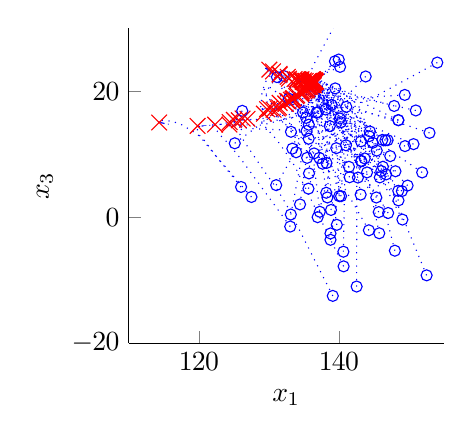
\begin{tikzpicture}

\begin{axis}[%
width=4cm,
height=4cm,
scale only axis,
xmin=110,
xmax=155,
xlabel={$x_1$},
ymin=-20,
ymax=30,
ylabel={$x_3$},
axis x line*=bottom,
axis y line*=left
]
\addplot [
color=blue,
dotted,
forget plot
]
table[row sep=crcr]{
133.35681987922 10.8841024888732\\
135.782024142063 18.3350084656896\\
135.57509347932 18.9040537944205\\
134.866483579293 20.3805414313985\\
134.476333455592 20.9618193556903\\
134.091538927312 21.5766940301034\\
134.011568443763 21.8255217930903\\
134.046057425386 21.8467627620992\\
134.091316154945 21.7950728965056\\
134.045091685323 21.7952002659453\\
134.206612301894 21.7975551420049\\
134.208853749002 21.7890653106618\\
134.189853293825 21.8032130333547\\
134.323186650354 21.797468353246\\
134.41293316264 21.7919281843479\\
134.390212651898 21.7950146669832\\
134.390667355101 21.8493839152079\\
134.499953805048 21.7833518952136\\
134.341012902163 21.7976524908878\\
134.308548350366 21.805836847949\\
134.31528742678 21.8045136108208\\
134.397781962528 21.7769867043344\\
134.371917940411 21.7772624288922\\
134.333783609591 21.7982576289909\\
134.24421436661 21.8225875921588\\
134.321290163699 21.797923490581\\
134.212270722605 21.8327027810045\\
134.174559958789 21.8272129207476\\
134.054378284642 21.8632364622274\\
133.946266826988 21.8804216426222\\
133.99267217835 21.8648495050247\\
134.00314288986 21.8697386406148\\
133.982128285993 21.877314279164\\
};
\addplot [
color=blue,
only marks,
mark=o,
mark options={solid},
forget plot
]
table[row sep=crcr]{
133.35681987922 10.8841024888732\\
};
\addplot [
color=red,
mark size=4.0pt,
only marks,
mark=x,
mark options={solid},
forget plot
]
table[row sep=crcr]{
133.982128285993 21.877314279164\\
};
\addplot [
color=blue,
dotted,
forget plot
]
table[row sep=crcr]{
133.160008391131 13.5599911393441\\
133.449478766983 19.8689745820507\\
133.144489919092 20.3918948351497\\
132.364704831709 21.5901002355652\\
131.88591675204 22.2089562770786\\
131.565103515987 22.6720108506258\\
131.473240449167 22.776181723731\\
131.487787146732 22.7572250981471\\
131.33431173094 22.858999452293\\
131.323181246468 22.8313881431084\\
131.133378072109 22.9458953427952\\
131.060462546266 23.0103746432949\\
131.097188610767 22.9574679341916\\
131.216578501029 22.9040673756242\\
130.871263564287 23.0665443901768\\
130.871172238185 23.0554893446539\\
130.561373722662 23.2235004667535\\
130.450298804616 23.2910943703734\\
130.370287591378 23.3416342276114\\
130.340050355482 23.3692979594318\\
130.708392081269 23.1668104922262\\
130.67160701893 23.1819054281433\\
130.874541146985 23.0790300119654\\
131.02699448289 22.9934901071988\\
130.859632276542 23.0945539005886\\
130.834980363136 23.1085937605101\\
130.788531822455 23.1134347318513\\
130.846654509879 23.0652256154693\\
131.127305194158 22.9225513261913\\
131.122453839847 22.9280920221196\\
131.08790554646 22.9583714926942\\
131.248971058486 22.8990583321476\\
131.526187511036 22.7605761442911\\
};
\addplot [
color=blue,
only marks,
mark=o,
mark options={solid},
forget plot
]
table[row sep=crcr]{
133.160008391131 13.5599911393441\\
};
\addplot [
color=red,
mark size=4.0pt,
only marks,
mark=x,
mark options={solid},
forget plot
]
table[row sep=crcr]{
131.526187511036 22.7605761442911\\
};
\addplot [
color=blue,
dotted,
forget plot
]
table[row sep=crcr]{
143.20680332871 8.87687295689003\\
135.235244071681 16.8942053308934\\
134.89533494454 17.3502081514563\\
133.461027592108 19.2169488849485\\
132.757542181983 20.043874841765\\
131.737433220973 21.1523979585777\\
131.123504220912 21.8713555033806\\
130.478005816325 22.6177090796799\\
130.121155117354 23.0760012827078\\
129.807216421995 23.3947309765173\\
129.731107721037 23.4744600108122\\
129.686099920016 23.5118463446882\\
129.352139701215 23.780759494488\\
129.560227576531 23.6765450025851\\
129.438874234221 23.7571945412585\\
129.631355382773 23.6481330780928\\
129.759194965519 23.5669602246332\\
129.740953871895 23.599872220905\\
129.445131653716 23.7815525081069\\
129.593419245559 23.690131144999\\
129.551143201341 23.6958136563596\\
129.533297350729 23.7110027215062\\
129.597315530746 23.7049162850313\\
129.726894211752 23.6204285351807\\
129.476946683294 23.7589980080704\\
129.566952606352 23.7036185684701\\
129.309679865832 23.8719424456827\\
129.452117480558 23.7863214380598\\
129.753290545194 23.6162720480936\\
129.477856882648 23.7891041246758\\
129.740396563773 23.6378601631169\\
129.746921159353 23.6343692145659\\
129.710757791667 23.657702360106\\
129.802166457792 23.6017264123619\\
129.455922313599 23.7938296866919\\
129.753270667566 23.6158032417238\\
129.845886301514 23.5600569233789\\
129.862477135031 23.5376396790938\\
129.851698022462 23.5455606590315\\
129.982389558789 23.4676580593803\\
129.574162321503 23.7007953627285\\
129.668567326594 23.6281745293068\\
129.719376822335 23.6035288274345\\
129.845726595208 23.5280551639142\\
130.030052518341 23.4177074415315\\
130.109846805455 23.3867473274397\\
130.025761923365 23.440825106366\\
130.073001675758 23.4217264366974\\
};
\addplot [
color=blue,
only marks,
mark=o,
mark options={solid},
forget plot
]
table[row sep=crcr]{
143.20680332871 8.87687295689003\\
};
\addplot [
color=red,
mark size=4.0pt,
only marks,
mark=x,
mark options={solid},
forget plot
]
table[row sep=crcr]{
130.073001675758 23.4217264366974\\
};
\addplot [
color=blue,
dotted,
forget plot
]
table[row sep=crcr]{
131.052986240617 5.09058887006587\\
136.769132569683 16.1638796328243\\
136.694000052856 16.6761688458786\\
136.097046730623 18.7971064680617\\
135.706429749464 19.6921919077987\\
135.400498915658 20.5574042513649\\
135.32303260151 20.7276291613816\\
135.357969775363 20.6558232947679\\
135.316928023246 20.6527530898506\\
135.559149975229 20.7294677636766\\
135.587451283836 20.7225428231096\\
135.762887042213 20.8438896048915\\
135.689812060863 20.72580731452\\
135.796881801555 20.8171013331091\\
135.831010742575 20.8044111592631\\
135.750775428774 20.7112982299106\\
135.815948330453 20.7561500983917\\
135.887402856826 20.8431893637085\\
135.880422234357 20.8400105264865\\
135.8755369688 20.8124888907155\\
135.854779381398 20.7859626890821\\
135.996580396927 20.9113080961945\\
136.11193723885 20.9934972728516\\
136.131793538172 21.0607612013205\\
136.129978721014 21.0530882727393\\
136.143323684285 21.1059518900153\\
136.288111202676 21.2337466360209\\
136.260889890625 21.2083264386561\\
136.35406875641 21.2204034838224\\
};
\addplot [
color=blue,
only marks,
mark=o,
mark options={solid},
forget plot
]
table[row sep=crcr]{
131.052986240617 5.09058887006587\\
};
\addplot [
color=red,
mark size=4.0pt,
only marks,
mark=x,
mark options={solid},
forget plot
]
table[row sep=crcr]{
136.35406875641 21.2204034838224\\
};
\addplot [
color=blue,
dotted,
forget plot
]
table[row sep=crcr]{
148.512736993562 15.3904813154739\\
140.500433916728 17.5613370473093\\
139.92579519574 17.8780954442517\\
138.249125006672 18.5282784339577\\
137.314253307051 18.8812897469503\\
136.310255332791 19.1430933148239\\
135.694128029056 19.3806466948105\\
135.320413388251 19.3819861378952\\
135.061439131878 19.3852739243448\\
134.906495317052 19.3808254231458\\
134.830843952877 19.3349745761559\\
134.80233261858 19.3446011072985\\
134.753359274065 19.3325483117418\\
134.667791938518 19.2865853424925\\
134.707674474782 19.2817435931247\\
134.660048864074 19.2728024024862\\
134.746380784734 19.3724015432573\\
134.6654023789 19.3120599231126\\
134.720271853585 19.3811393822452\\
134.697544457098 19.36905980241\\
134.81420604901 19.4693537524632\\
134.869047374551 19.543692818667\\
134.921441029399 19.6019646596035\\
134.958778070813 19.6267235640126\\
134.901137915199 19.5959531543688\\
134.830430553051 19.5590164093309\\
134.839945086601 19.5622972385292\\
134.93005568732 19.6496359310434\\
134.950430058007 19.6805538884448\\
135.069771847784 19.7792175796452\\
135.030471258535 19.7673642390745\\
134.991549631385 19.7442368655288\\
135.071814537628 19.8011763595663\\
135.005121289065 19.7366971129458\\
135.020442474514 19.7540736447335\\
135.01023319416 19.7633559784229\\
134.951955082193 19.7085516327754\\
135.031751510473 19.7781527022615\\
134.987025266896 19.7085429097382\\
134.851738416172 19.634791503933\\
134.909492449524 19.6772915548511\\
134.801114511916 19.6345258691261\\
134.759692595587 19.6074880519801\\
134.808104223171 19.6599196407939\\
134.790038050889 19.6587378219124\\
134.647765817105 19.5394136092559\\
134.615777077518 19.5135423507279\\
};
\addplot [
color=blue,
only marks,
mark=o,
mark options={solid},
forget plot
]
table[row sep=crcr]{
148.512736993562 15.3904813154739\\
};
\addplot [
color=red,
mark size=4.0pt,
only marks,
mark=x,
mark options={solid},
forget plot
]
table[row sep=crcr]{
134.615777077518 19.5135423507279\\
};
\addplot [
color=blue,
dotted,
forget plot
]
table[row sep=crcr]{
151.906798640258 7.1052098635708\\
141.792448570141 14.8015860974617\\
141.370193745236 15.348990661548\\
139.86632956315 17.3437027494923\\
139.049544660557 18.3996882908444\\
138.158057453392 19.4358215311757\\
137.485173711019 20.3218233114798\\
137.001122606493 20.9254627840571\\
136.787748540759 21.2676670198431\\
136.697595043522 21.3955434701856\\
136.616436511598 21.5069436790044\\
136.598317162897 21.5873306155225\\
136.50364693295 21.6414157896254\\
136.47192288021 21.6681650058447\\
136.494460812277 21.6652934709388\\
136.527777594046 21.6549945430499\\
136.47156757339 21.6980182700856\\
136.464396730428 21.6775970106855\\
136.434112987683 21.7010709013654\\
136.464143776187 21.714154664906\\
136.526205143631 21.6803639958699\\
136.523300023519 21.6545268100202\\
136.520027663356 21.6645999521664\\
};
\addplot [
color=blue,
only marks,
mark=o,
mark options={solid},
forget plot
]
table[row sep=crcr]{
151.906798640258 7.1052098635708\\
};
\addplot [
color=red,
mark size=4.0pt,
only marks,
mark=x,
mark options={solid},
forget plot
]
table[row sep=crcr]{
136.520027663356 21.6645999521664\\
};
\addplot [
color=blue,
dotted,
forget plot
]
table[row sep=crcr]{
140.053745570725 3.34201234577398\\
139.648301731597 12.1961189619945\\
139.439042587461 12.9061466922868\\
138.653069109721 15.0602749273854\\
138.098197728534 16.2925025252176\\
137.543939757003 17.6273565665581\\
137.045888906914 18.7394245065451\\
136.677889705923 19.5108382030201\\
136.580226236197 19.9713629174016\\
136.511112448775 20.2291080125046\\
136.410152764339 20.4685400935543\\
136.389165397134 20.6025195416407\\
136.351841319653 20.7356746782527\\
136.242919572448 20.8360360835318\\
136.238857488331 20.8962149349967\\
136.244684825996 20.9323392363758\\
136.301268803329 21.0114999102428\\
136.300428659625 21.048890344061\\
136.232379482981 21.0815525015906\\
136.189160840509 21.1055712988425\\
136.143675205944 21.1088610148751\\
136.078003343325 21.1225777644543\\
135.979397145413 21.1398009093369\\
135.990689285694 21.1347020070727\\
135.991783046264 21.1542091193352\\
136.123462793211 21.1789129104874\\
136.113587286424 21.1923572776004\\
136.206076349176 21.1860713247546\\
136.174264595805 21.1953041135426\\
136.215674415091 21.2176812929882\\
136.187049103282 21.2671269388858\\
136.112195770605 21.2382201386713\\
136.068118011354 21.2338689465609\\
136.050384522379 21.257017245011\\
136.04356471359 21.241183988439\\
136.019542857237 21.2542025120454\\
135.941229140592 21.2758535630938\\
135.946870026278 21.2732494873411\\
135.995495141977 21.259227057612\\
136.009354813969 21.2519205486615\\
136.02148524263 21.2566621886669\\
135.971638231243 21.279794849391\\
135.975678604238 21.2799054626262\\
136.045596637463 21.2793591449809\\
136.066271064499 21.2839893504678\\
136.094445911949 21.30605764635\\
};
\addplot [
color=blue,
only marks,
mark=o,
mark options={solid},
forget plot
]
table[row sep=crcr]{
140.053745570725 3.34201234577398\\
};
\addplot [
color=red,
mark size=4.0pt,
only marks,
mark=x,
mark options={solid},
forget plot
]
table[row sep=crcr]{
136.094445911949 21.30605764635\\
};
\addplot [
color=blue,
dotted,
forget plot
]
table[row sep=crcr]{
144.440883612646 13.6073336481048\\
139.865243333028 19.3894057294508\\
139.434761426767 19.8178949004829\\
138.103841814098 20.890030036249\\
137.473673969363 21.3202704099808\\
136.853006498686 21.6691106330355\\
136.686068225218 21.7518034426351\\
136.619517602502 21.7781275158887\\
136.608903084677 21.776488496718\\
136.563881194097 21.7995471463482\\
136.533852694694 21.8293023811708\\
136.564184181348 21.7769285323554\\
136.572987891828 21.7492297320801\\
136.53363723059 21.8110487031099\\
136.540534340263 21.7780875718528\\
136.497214158823 21.8134802621056\\
136.519342534158 21.8111748295313\\
136.485119570677 21.8442489958538\\
136.480152614308 21.8396991256253\\
136.478495616728 21.8270471584371\\
136.464180544121 21.8306682965317\\
136.48171878492 21.8090712853838\\
136.483385539617 21.7980033663115\\
136.471541970794 21.8174251148982\\
136.474741695899 21.8133223326696\\
136.48716658592 21.7899455335536\\
136.486688300291 21.7870847573493\\
136.491387334896 21.7924566822186\\
136.498449699438 21.752001196139\\
136.498730571158 21.7435827523571\\
136.497212700815 21.7358618088181\\
136.47610881871 21.7592174174864\\
136.484558395975 21.7543924732638\\
136.470812492999 21.764748330727\\
136.453737847106 21.7496480226846\\
136.455964127174 21.7474333786533\\
136.446315914005 21.7282718542757\\
136.465480278569 21.7209612800237\\
136.39550114631 21.7383975057532\\
136.346372038353 21.7404196363215\\
136.321318362308 21.7385056845697\\
};
\addplot [
color=blue,
only marks,
mark=o,
mark options={solid},
forget plot
]
table[row sep=crcr]{
144.440883612646 13.6073336481048\\
};
\addplot [
color=red,
mark size=4.0pt,
only marks,
mark=x,
mark options={solid},
forget plot
]
table[row sep=crcr]{
136.321318362308 21.7385056845697\\
};
\addplot [
color=blue,
dotted,
forget plot
]
table[row sep=crcr]{
138.707108444427 14.4605653155275\\
137.517068901658 19.1419341399151\\
137.148861970189 19.748119939597\\
136.377164325071 20.8444598534001\\
136.026095771031 21.285889472532\\
136.079464452594 21.4586860822816\\
136.110883568672 21.5647536299053\\
136.198330372934 21.6238438845911\\
136.284820495282 21.6037126792987\\
136.325039481777 21.5728570294027\\
136.343808512852 21.5472742321351\\
136.337308666711 21.5024297102643\\
136.383006526229 21.4867193883965\\
136.366991103322 21.5231687633102\\
136.410746459891 21.5542183289499\\
136.463686306669 21.6240580999763\\
136.439683306895 21.6286737028111\\
136.445821045678 21.6332971446531\\
136.429330691866 21.6394463126636\\
136.448110355015 21.6820382011676\\
136.463694291238 21.6786341566361\\
136.493327906379 21.6621096374548\\
136.495176053848 21.6586897185579\\
};
\addplot [
color=blue,
only marks,
mark=o,
mark options={solid},
forget plot
]
table[row sep=crcr]{
138.707108444427 14.4605653155275\\
};
\addplot [
color=red,
mark size=4.0pt,
only marks,
mark=x,
mark options={solid},
forget plot
]
table[row sep=crcr]{
136.495176053848 21.6586897185579\\
};
\addplot [
color=blue,
dotted,
forget plot
]
table[row sep=crcr]{
148.493253261674 4.18802879860039\\
141.994019826264 15.5299046904358\\
141.637476116622 16.0368971549345\\
140.183942233046 17.9042296711462\\
139.381909324717 18.796582053405\\
138.43652302229 19.8003825159516\\
137.697652944704 20.4875898154129\\
137.217324762828 20.9039474881068\\
136.685517902574 21.383251076664\\
136.684458549664 21.4500687415276\\
136.659732054973 21.466475187437\\
136.647795473594 21.4781685941911\\
136.654117146467 21.4602061781976\\
136.676924144314 21.4723825939268\\
136.712215797662 21.4694454327953\\
136.710591078135 21.4606920177547\\
136.720084962626 21.4261440676166\\
136.717496924846 21.4328624772352\\
136.710701621247 21.4325526175699\\
136.708726367165 21.4663812227815\\
136.684766582361 21.5035262962023\\
136.65353164082 21.5563044134676\\
};
\addplot [
color=blue,
only marks,
mark=o,
mark options={solid},
forget plot
]
table[row sep=crcr]{
148.493253261674 4.18802879860039\\
};
\addplot [
color=red,
mark size=4.0pt,
only marks,
mark=x,
mark options={solid},
forget plot
]
table[row sep=crcr]{
136.65353164082 21.5563044134676\\
};
\addplot [
color=blue,
dotted,
forget plot
]
table[row sep=crcr]{
147.904353571163 17.6587971110626\\
140.001203228409 20.1035596260969\\
139.617804887346 20.3610145189852\\
138.114569636093 21.2681335139423\\
137.529218078131 21.5166814207351\\
136.887897915007 21.6960838995029\\
136.690523095953 21.7180316997077\\
136.656648097893 21.6719488720284\\
136.624340603811 21.6651891133315\\
136.586000549347 21.6929283897238\\
136.625484973734 21.6609667493241\\
136.660762306705 21.6576671280954\\
136.665370446876 21.6543733843069\\
136.633480062327 21.7060710378836\\
136.577467834127 21.7475832412873\\
136.580631238645 21.7568170209064\\
136.55320763743 21.7550056515172\\
136.539410943685 21.7738653805241\\
136.573616577576 21.7408455051924\\
136.581983644356 21.7424179027951\\
136.611154015802 21.750472930963\\
136.615048398587 21.7514393561894\\
136.615654235039 21.7350284818479\\
136.624881435709 21.702688403039\\
};
\addplot [
color=blue,
only marks,
mark=o,
mark options={solid},
forget plot
]
table[row sep=crcr]{
147.904353571163 17.6587971110626\\
};
\addplot [
color=red,
mark size=4.0pt,
only marks,
mark=x,
mark options={solid},
forget plot
]
table[row sep=crcr]{
136.624881435709 21.702688403039\\
};
\addplot [
color=blue,
dotted,
forget plot
]
table[row sep=crcr]{
146.222126709961 12.2775971359114\\
140.650439788368 17.825266497131\\
140.2142510488 18.3094958067393\\
138.874805961801 19.6457370572403\\
138.113812151319 20.3065718615453\\
137.438497358016 20.9470530301093\\
136.981739210715 21.2469066758009\\
136.810990676361 21.3773612223516\\
136.759345875462 21.4174371036749\\
136.692402390356 21.4593855274275\\
136.710059797642 21.4771368737123\\
136.70548571576 21.4763064037857\\
136.693194022673 21.4970977261304\\
136.676637140397 21.5054746041669\\
136.693797172392 21.4927099778997\\
136.681031705252 21.5086383072555\\
136.685748974635 21.4761687244504\\
136.673705307606 21.4846858379119\\
136.642715452646 21.5032978073848\\
136.643742062452 21.5056036778593\\
136.611220797468 21.5384267983231\\
136.617059565105 21.5146404814941\\
136.614881035475 21.4776406907969\\
136.604090779159 21.4618127981378\\
};
\addplot [
color=blue,
only marks,
mark=o,
mark options={solid},
forget plot
]
table[row sep=crcr]{
146.222126709961 12.2775971359114\\
};
\addplot [
color=red,
mark size=4.0pt,
only marks,
mark=x,
mark options={solid},
forget plot
]
table[row sep=crcr]{
136.604090779159 21.4618127981378\\
};
\addplot [
color=blue,
dotted,
forget plot
]
table[row sep=crcr]{
152.957003818275 13.3843009194259\\
141.913485401573 17.4931451610916\\
141.519785943697 17.8618965363057\\
139.791270232482 19.1734176132841\\
138.901856810221 19.8454006000655\\
137.993455393843 20.4730504218173\\
137.388827439686 20.8924467278293\\
136.929410772471 21.2018287131847\\
136.790671592794 21.2865955918506\\
136.655653508561 21.335617864279\\
136.577568348169 21.3627343646783\\
136.469693522774 21.3161879363619\\
136.44831768498 21.2881674941332\\
136.442764560463 21.3056098863052\\
136.453433166087 21.3327806311238\\
136.462179521449 21.3463941523822\\
136.43759363627 21.3117935019599\\
136.454086461349 21.2465554669397\\
136.484508158269 21.2080153025134\\
136.466849591824 21.1943271204253\\
136.502093187085 21.268826634524\\
136.478388749938 21.3021393079629\\
136.451974341364 21.2918104982775\\
136.450679592018 21.2799103400538\\
136.446160738944 21.2578238416742\\
136.503297880298 21.317601891336\\
136.475111998762 21.3008447866059\\
136.485971870414 21.296664768155\\
136.448828896093 21.2520226577643\\
136.466334345173 21.2686523721208\\
136.453331558674 21.253255166117\\
};
\addplot [
color=blue,
only marks,
mark=o,
mark options={solid},
forget plot
]
table[row sep=crcr]{
152.957003818275 13.3843009194259\\
};
\addplot [
color=red,
mark size=4.0pt,
only marks,
mark=x,
mark options={solid},
forget plot
]
table[row sep=crcr]{
136.453331558674 21.253255166117\\
};
\addplot [
color=blue,
dotted,
forget plot
]
table[row sep=crcr]{
133.140938029048 0.423893685163373\\
134.85650994314 10.3596674903798\\
134.611210276952 10.9667925321144\\
133.553988089068 13.0808892308164\\
132.740453313 14.2068567999667\\
131.855337158509 15.2491814798711\\
131.27608437178 15.9905962092909\\
130.965584264481 16.4650453323197\\
130.877090659993 16.6620525163536\\
130.777303306117 16.7217290436228\\
130.571473593332 16.7586161311988\\
130.651713433972 16.8851440772025\\
131.044966848204 17.0853458980455\\
130.976770004314 17.0964704416748\\
131.030585586291 17.1790487544809\\
131.094415895654 17.2043805533386\\
131.224670238508 17.2362294798439\\
131.04389121119 17.1730698368538\\
131.178837313938 17.2493819996083\\
131.603562240126 17.4589899618486\\
131.380730680203 17.3520201449807\\
131.237753475092 17.2545119894278\\
131.264719412586 17.293498128399\\
131.186778838468 17.2838367132672\\
131.452038038645 17.4215437090147\\
};
\addplot [
color=blue,
only marks,
mark=o,
mark options={solid},
forget plot
]
table[row sep=crcr]{
133.140938029048 0.423893685163373\\
};
\addplot [
color=red,
mark size=4.0pt,
only marks,
mark=x,
mark options={solid},
forget plot
]
table[row sep=crcr]{
131.452038038645 17.4215437090147\\
};
\addplot [
color=blue,
dotted,
forget plot
]
table[row sep=crcr]{
141.450900185129 7.99655600290338\\
133.323905922782 14.4434379269866\\
132.940171118768 14.9370316399587\\
131.542364478063 16.4268309889025\\
131.095362273191 17.007886717109\\
130.912656090578 17.4009719079748\\
131.091362659034 17.5854619511773\\
131.037074035237 17.555395224643\\
131.007969265499 17.517275240159\\
131.036213033332 17.4829570919446\\
131.218166252208 17.4454788366715\\
130.90125311612 17.2926071104624\\
130.777006287422 17.2177147441736\\
130.90344730211 17.2455728255357\\
131.023107192272 17.3436053863652\\
130.753808294442 17.1925947620499\\
130.750654907173 17.187101686516\\
130.56614374019 17.1209585735607\\
130.054913317321 16.77832229734\\
130.671479358298 17.0608999578385\\
};
\addplot [
color=blue,
only marks,
mark=o,
mark options={solid},
forget plot
]
table[row sep=crcr]{
141.450900185129 7.99655600290338\\
};
\addplot [
color=red,
mark size=4.0pt,
only marks,
mark=x,
mark options={solid},
forget plot
]
table[row sep=crcr]{
130.671479358298 17.0608999578385\\
};
\addplot [
color=blue,
dotted,
forget plot
]
table[row sep=crcr]{
134.884569833816 16.6145948545627\\
127.637699556941 15.4147925596201\\
127.22553210911 15.4261758192467\\
125.797937962182 15.5052159327534\\
125.152871592007 15.4697606538607\\
125.181124012828 15.4211222871642\\
125.422421312128 15.3642584260906\\
125.478621683467 15.3839951131144\\
125.716392843703 15.455812121312\\
125.308867018717 15.3793356556685\\
125.352621036443 15.4496845548011\\
125.151265203294 15.4310453536618\\
125.369012206007 15.4976280009695\\
125.588287894732 15.5228331696302\\
125.608384566315 15.5426608879474\\
125.556301859876 15.5281570259519\\
125.480801721375 15.5047495118433\\
125.680451089546 15.5551021683341\\
125.945775786211 15.6295530512955\\
125.754594031834 15.5730689870945\\
126.405587904426 15.7416229915988\\
126.463456856347 15.740425987963\\
126.248465739532 15.6639039377817\\
};
\addplot [
color=blue,
only marks,
mark=o,
mark options={solid},
forget plot
]
table[row sep=crcr]{
134.884569833816 16.6145948545627\\
};
\addplot [
color=red,
mark size=4.0pt,
only marks,
mark=x,
mark options={solid},
forget plot
]
table[row sep=crcr]{
126.248465739532 15.6639039377817\\
};
\addplot [
color=blue,
dotted,
forget plot
]
table[row sep=crcr]{
138.096450518276 17.0984626757134\\
128.905828748532 14.6111971446991\\
128.388599021106 14.6316423648525\\
126.529945953373 14.664486227254\\
125.731210557318 14.8377176299928\\
125.252530635592 14.9754386327099\\
124.5911904149 14.9692649615023\\
125.246980796857 15.1404781426845\\
125.641441859512 15.2746498761538\\
125.621516439579 15.2701288099438\\
125.748127080504 15.3599063430865\\
126.251718962182 15.5423341696421\\
126.542831818605 15.5754945000444\\
126.212055468718 15.4617923264901\\
126.66297158896 15.570477755611\\
126.515744807969 15.5057140727406\\
126.50667100614 15.4996760701592\\
126.940309856304 15.6122887913648\\
126.947282491398 15.6154597671475\\
};
\addplot [
color=blue,
only marks,
mark=o,
mark options={solid},
forget plot
]
table[row sep=crcr]{
138.096450518276 17.0984626757134\\
};
\addplot [
color=red,
mark size=4.0pt,
only marks,
mark=x,
mark options={solid},
forget plot
]
table[row sep=crcr]{
126.947282491398 15.6154597671475\\
};
\addplot [
color=blue,
dotted,
forget plot
]
table[row sep=crcr]{
139.136463682346 -12.4916162733161\\
132.818916305362 1.3645160205038\\
132.459274333766 2.08077885031918\\
131.030246031888 4.72107155500598\\
130.042996654526 6.22608774970005\\
128.96468876213 7.92596053484299\\
127.987401728797 9.53673836287025\\
127.125513435002 10.9419784219689\\
126.477210359182 12.0188527768657\\
126.135222404201 12.716997135028\\
125.876181550275 13.1333046431272\\
126.040496284 13.4800208021185\\
126.153563769412 13.6946637666746\\
125.965674828728 13.8396768989045\\
126.217710156235 14.0680477035335\\
126.408222106495 14.246565686453\\
126.494474765105 14.3511279476418\\
126.37809765002 14.4296839955338\\
126.181815131684 14.4321313728911\\
126.04348073492 14.5138137467427\\
125.80298640105 14.5115284868024\\
125.650634539718 14.4998789455873\\
125.790383704201 14.5649671984939\\
125.744839064869 14.5721474001727\\
125.868115567101 14.6249032026908\\
125.832877502641 14.6498708461342\\
125.781687666349 14.6625100822209\\
125.738044673691 14.6454079065665\\
125.609289622407 14.6223883992046\\
125.569345626496 14.6080300173855\\
125.518541697621 14.6379168593498\\
125.588632963195 14.690254136804\\
125.38019525427 14.6524050434246\\
125.285776663335 14.6524308619897\\
125.019597124499 14.6070479730181\\
125.058950381958 14.6274688435642\\
124.624305769652 14.5468347730864\\
124.335318593778 14.4863880401174\\
124.461140169293 14.5159501679746\\
124.463087613012 14.5241469085168\\
124.348815481575 14.5022392436001\\
124.2217555071 14.4907092312328\\
124.225741767559 14.4909066413904\\
124.344523219871 14.533041171703\\
124.195133988203 14.5296777018943\\
123.983287439993 14.5022186673524\\
124.061177267123 14.5351939267302\\
124.003972955619 14.5556102869982\\
123.975185464376 14.5677050087832\\
124.002325059047 14.5907160404878\\
124.047144645911 14.6108392742034\\
123.875185196989 14.5871450880881\\
123.929203895127 14.580255288868\\
123.719050845225 14.5524672147071\\
124.040412601458 14.6167385738871\\
124.040563353826 14.6167162498932\\
124.16870087752 14.644643856689\\
124.195680913872 14.6544349562844\\
124.270908721369 14.6763630449104\\
124.382217015852 14.6952209263473\\
124.596883356891 14.7368302599982\\
124.469274076304 14.7218357169521\\
124.366356756327 14.7109040797072\\
};
\addplot [
color=blue,
only marks,
mark=o,
mark options={solid},
forget plot
]
table[row sep=crcr]{
139.136463682346 -12.4916162733161\\
};
\addplot [
color=red,
mark size=4.0pt,
only marks,
mark=x,
mark options={solid},
forget plot
]
table[row sep=crcr]{
124.366356756327 14.7109040797072\\
};
\addplot [
color=blue,
dotted,
forget plot
]
table[row sep=crcr]{
126.201955654672 16.8871518357841\\
124.805309616399 15.1163425675002\\
124.888692385015 15.4269167176387\\
124.935682459079 15.5131214625906\\
125.243272288487 15.5310297016916\\
125.337983342316 15.4766490589948\\
125.806449862638 15.6353236124596\\
125.524560862432 15.5942654078857\\
125.531277496672 15.6069173937454\\
125.303502248126 15.5531503469429\\
125.089903179904 15.5156135334585\\
124.762372473723 15.404748295423\\
124.520257859857 15.3452496276435\\
125.262855090882 15.515902176238\\
125.010081365321 15.4453112565398\\
};
\addplot [
color=blue,
only marks,
mark=o,
mark options={solid},
forget plot
]
table[row sep=crcr]{
126.201955654672 16.8871518357841\\
};
\addplot [
color=red,
mark size=4.0pt,
only marks,
mark=x,
mark options={solid},
forget plot
]
table[row sep=crcr]{
125.010081365321 15.4453112565398\\
};
\addplot [
color=blue,
dotted,
forget plot
]
table[row sep=crcr]{
139.487752632874 20.4466722484334\\
132.720828337788 15.6945328351423\\
132.016282059625 15.5177779797163\\
130.034982554739 15.218370256307\\
128.986428004355 15.3005496057855\\
128.231933120526 15.5053591745869\\
127.564726543768 15.5422081337858\\
126.911737910466 15.3730239873954\\
126.740639018516 15.4568160899308\\
126.454429051817 15.4357254132262\\
126.138985981571 15.4042460995135\\
126.316441404773 15.476764509282\\
126.425894693376 15.5175648502347\\
126.198983065469 15.470126204589\\
126.287162342371 15.5132773599795\\
126.04017891141 15.4412774441459\\
126.103166639486 15.4627258035288\\
125.703840514416 15.3883462412191\\
};
\addplot [
color=blue,
only marks,
mark=o,
mark options={solid},
forget plot
]
table[row sep=crcr]{
139.487752632874 20.4466722484334\\
};
\addplot [
color=red,
mark size=4.0pt,
only marks,
mark=x,
mark options={solid},
forget plot
]
table[row sep=crcr]{
125.703840514416 15.3883462412191\\
};
\addplot [
color=blue,
dotted,
forget plot
]
table[row sep=crcr]{
127.514736695982 3.21104152442964\\
122.27756685408 9.92731881462103\\
121.858537600854 10.6274903851992\\
120.741153925957 12.2505616500995\\
119.892696640722 13.2052078251658\\
119.800712342504 13.8701931991109\\
119.658253608467 14.1523911830742\\
119.979217970126 14.2971827676232\\
119.802692560044 14.3500350340281\\
120.233507086327 14.4116044317753\\
119.836174272696 14.369928581975\\
120.029801822183 14.3980480633381\\
120.448516167323 14.4241840428704\\
120.220987915672 14.4187024347217\\
120.386158066379 14.4398492449307\\
120.524024680298 14.4864748059584\\
120.175754696185 14.4669282402774\\
120.195214632258 14.5133814808028\\
119.757773007379 14.4982472843014\\
120.195023215733 14.5048450797893\\
120.000223759769 14.5134537919327\\
119.823045061226 14.4942115604085\\
};
\addplot [
color=blue,
only marks,
mark=o,
mark options={solid},
forget plot
]
table[row sep=crcr]{
127.514736695982 3.21104152442964\\
};
\addplot [
color=red,
mark size=4.0pt,
only marks,
mark=x,
mark options={solid},
forget plot
]
table[row sep=crcr]{
119.823045061226 14.4942115604085\\
};
\addplot [
color=blue,
dotted,
forget plot
]
table[row sep=crcr]{
138.965966654712 17.8272866905193\\
134.703261591021 18.9926947218371\\
134.150494574926 19.116644062052\\
133.162737149118 18.9071589049104\\
132.600917496034 18.6811264779745\\
132.511561208206 18.6552778955655\\
132.386648229104 18.4745014861552\\
132.486968198696 18.4819541542558\\
132.278556192056 18.3799110142602\\
132.161768736893 18.3418418983441\\
131.986511576826 18.2104915051794\\
132.267016962701 18.2535036307424\\
132.158705269825 18.2102056026127\\
132.157696558329 18.1856990595235\\
132.460593458563 18.3460184271584\\
132.147182891309 18.1511203353575\\
132.411336713901 18.2894444711274\\
132.304191037143 18.2296656589066\\
132.408811739996 18.2935422978808\\
132.73474355817 18.5009204866406\\
132.620808615886 18.4796767633624\\
132.603273751042 18.4669163376964\\
132.604470009486 18.4700402393568\\
};
\addplot [
color=blue,
only marks,
mark=o,
mark options={solid},
forget plot
]
table[row sep=crcr]{
138.965966654712 17.8272866905193\\
};
\addplot [
color=red,
mark size=4.0pt,
only marks,
mark=x,
mark options={solid},
forget plot
]
table[row sep=crcr]{
132.604470009486 18.4700402393568\\
};
\addplot [
color=blue,
dotted,
forget plot
]
table[row sep=crcr]{
151.000417341045 16.9445999516813\\
142.835793365477 18.9714963972081\\
142.364131625273 19.2434223861179\\
140.62243678046 20.0985581180154\\
139.7499719746 20.547314433434\\
138.77126735104 20.9190397571417\\
138.064991925236 21.2060025987591\\
137.555643121928 21.3864154461138\\
137.335692873603 21.5066281982213\\
137.190992107652 21.5254686838428\\
137.076026931938 21.557882292215\\
137.057906130256 21.5621158073849\\
137.052582391988 21.597099296817\\
136.977001217023 21.6178077551825\\
136.908183330153 21.6310724377815\\
136.859567327311 21.6146793240278\\
136.825527569458 21.6317390382884\\
136.807997750015 21.6204156938469\\
136.791054575446 21.6183233675191\\
136.780042266649 21.6190903288472\\
136.771877600044 21.6531366352989\\
136.754086687226 21.668741937674\\
136.725414606464 21.6858091223226\\
136.703601982947 21.7192934271523\\
136.674090079907 21.7335217821081\\
136.710538264025 21.7130879299658\\
136.72289486174 21.7239529141499\\
136.695317698861 21.7325342178587\\
136.681042364883 21.74655918358\\
136.643912580125 21.7653811088259\\
136.652394959041 21.7498152816504\\
136.629967954167 21.7258508093192\\
136.631719711888 21.6968085508605\\
136.644045958998 21.6962986733397\\
136.619877408237 21.7103738283351\\
136.610632390514 21.6932999285671\\
136.605085480613 21.6950940992401\\
136.597019176578 21.7037801916829\\
};
\addplot [
color=blue,
only marks,
mark=o,
mark options={solid},
forget plot
]
table[row sep=crcr]{
151.000417341045 16.9445999516813\\
};
\addplot [
color=red,
mark size=4.0pt,
only marks,
mark=x,
mark options={solid},
forget plot
]
table[row sep=crcr]{
136.597019176578 21.7037801916829\\
};
\addplot [
color=blue,
dotted,
forget plot
]
table[row sep=crcr]{
139.986618811135 25.0264409762746\\
135.597546539431 20.1428903009167\\
135.003882891517 19.6132550062905\\
133.609326688654 18.6490499068748\\
132.785649807011 18.2899128820377\\
132.555015925189 18.0337996369595\\
132.498373674673 18.0903054026251\\
132.567108505515 18.2031226145939\\
132.319046461443 18.0673253540282\\
132.085614728701 17.8705393877919\\
132.07009663136 17.8946783752456\\
132.067454957777 17.9016259931772\\
132.000777606419 17.8865674978161\\
131.893353413213 17.8319889228815\\
131.746839130417 17.7588123080992\\
131.618128415237 17.6449912535971\\
131.451399503705 17.5688508738051\\
131.48869526457 17.6265711300053\\
131.566626859044 17.650586655191\\
131.753012966279 17.76452838444\\
131.873022487893 17.8325973010827\\
132.324909042905 18.0536905008166\\
};
\addplot [
color=blue,
only marks,
mark=o,
mark options={solid},
forget plot
]
table[row sep=crcr]{
139.986618811135 25.0264409762746\\
};
\addplot [
color=red,
mark size=4.0pt,
only marks,
mark=x,
mark options={solid},
forget plot
]
table[row sep=crcr]{
132.324909042905 18.0536905008166\\
};
\addplot [
color=blue,
dotted,
forget plot
]
table[row sep=crcr]{
131.159153652717 22.2430999686153\\
129.672995450058 20.060394566458\\
129.639599887846 19.4463563432491\\
130.236451602356 18.5464946007963\\
130.727099270266 18.1973748001736\\
130.805140634192 17.9257992278321\\
130.672215266555 17.7355624101517\\
130.51910659277 17.6364124273181\\
130.093558008827 17.3631818387129\\
130.093702319154 17.3337757131365\\
130.138916900062 17.3468300504836\\
130.373988892462 17.4470390834553\\
130.643426705225 17.5602929381797\\
130.563885456295 17.5242661695451\\
130.938665226513 17.7183783559921\\
130.675607504229 17.5464895995829\\
130.657936956579 17.5354867692897\\
130.515610106161 17.4497962698326\\
130.462866434999 17.4142700256246\\
130.338732890789 17.3599389228781\\
130.417202063278 17.4197974304289\\
130.398845664018 17.3840143700672\\
130.572599285336 17.4617384902302\\
130.44632274997 17.385385878054\\
130.150622517275 17.2547648670175\\
130.181829839524 17.2675477893229\\
};
\addplot [
color=blue,
only marks,
mark=o,
mark options={solid},
forget plot
]
table[row sep=crcr]{
131.159153652717 22.2430999686153\\
};
\addplot [
color=red,
mark size=4.0pt,
only marks,
mark=x,
mark options={solid},
forget plot
]
table[row sep=crcr]{
130.181829839524 17.2675477893229\\
};
\addplot [
color=blue,
dotted,
forget plot
]
table[row sep=crcr]{
146.066746798992 7.33368269357982\\
137.636445480138 14.5227688848146\\
137.171249431223 14.9861744973778\\
135.592582776623 16.3660674806241\\
134.800992463888 17.062246886508\\
133.867777253076 17.7201544698671\\
133.282470784701 18.052324525465\\
133.039426209948 18.1846795245694\\
132.781692529087 18.2297343737006\\
132.65745748718 18.2015678135663\\
132.617747008288 18.2490793714952\\
132.509623764615 18.2493374298298\\
132.776772282957 18.3551238154484\\
132.585511606134 18.238886666833\\
132.715631070583 18.3230714688993\\
133.102640422147 18.5345678936187\\
132.940587866002 18.4464835733523\\
133.318885575484 18.7164771950755\\
133.516235505542 18.817902739377\\
133.402142018891 18.7471286510521\\
133.310802070227 18.6957020289428\\
133.203554034458 18.6437603128409\\
133.152003618783 18.6367872097347\\
133.078970312311 18.606910894427\\
133.238124037331 18.6872611161222\\
133.419403424505 18.8170734632707\\
133.226621993639 18.6827153981149\\
133.177804615921 18.6648032293251\\
133.15316433749 18.6501394711524\\
};
\addplot [
color=blue,
only marks,
mark=o,
mark options={solid},
forget plot
]
table[row sep=crcr]{
146.066746798992 7.33368269357982\\
};
\addplot [
color=red,
mark size=4.0pt,
only marks,
mark=x,
mark options={solid},
forget plot
]
table[row sep=crcr]{
133.15316433749 18.6501394711524\\
};
\addplot [
color=blue,
dotted,
forget plot
]
table[row sep=crcr]{
137.282036267629 0.86385338704678\\
136.105998343143 11.5575592917128\\
135.897926009407 12.1449086519624\\
134.875140860497 14.2253174061338\\
134.33198633245 15.2741397202354\\
133.766334707003 16.4610294247237\\
133.369315341569 17.123091210058\\
132.907714812592 17.6261464705114\\
133.174608981276 18.0198096136735\\
133.27277317064 18.3140763133084\\
133.238782857256 18.3037902214507\\
133.242943491277 18.4027830472496\\
132.987705482888 18.2210511650062\\
133.292216663928 18.4319096353783\\
133.330505698652 18.5056052188298\\
133.464703229465 18.5839916266298\\
133.372127936078 18.5598245034602\\
133.334088341629 18.5251075653491\\
};
\addplot [
color=blue,
only marks,
mark=o,
mark options={solid},
forget plot
]
table[row sep=crcr]{
137.282036267629 0.86385338704678\\
};
\addplot [
color=red,
mark size=4.0pt,
only marks,
mark=x,
mark options={solid},
forget plot
]
table[row sep=crcr]{
133.334088341629 18.5251075653491\\
};
\addplot [
color=blue,
dotted,
forget plot
]
table[row sep=crcr]{
135.333166112135 15.7697378118066\\
130.414320579106 20.4685184046411\\
130.034820777337 20.6552296795317\\
129.328923995092 20.2364670052949\\
129.638437893819 19.2826605942491\\
129.842319834589 18.7131763632023\\
129.764556331472 18.3275598921977\\
129.674260313153 18.0527009755049\\
129.908154391435 18.0257008802324\\
130.207629911366 18.0908753026263\\
130.35957605545 18.0830993061566\\
130.343314080151 17.9919588994148\\
130.468599004263 18.0124269100834\\
130.581137953601 17.9852354571218\\
130.867659501637 18.0781365998578\\
131.006609254323 18.1075933624404\\
130.709848682408 17.9138441644799\\
130.745761562513 17.8991226213718\\
130.632831764684 17.810316186225\\
130.732680677364 17.8348930593223\\
130.805626028621 17.8768772282458\\
131.176132948886 18.0082518311848\\
131.197661907086 17.9922462717386\\
131.296973607237 18.029638115502\\
131.323076276818 18.0096661648613\\
131.620739897726 18.1858752753174\\
131.635712702731 18.2044577744258\\
131.542743555732 18.1433540605257\\
};
\addplot [
color=blue,
only marks,
mark=o,
mark options={solid},
forget plot
]
table[row sep=crcr]{
135.333166112135 15.7697378118066\\
};
\addplot [
color=red,
mark size=4.0pt,
only marks,
mark=x,
mark options={solid},
forget plot
]
table[row sep=crcr]{
131.542743555732 18.1433540605257\\
};
\addplot [
color=blue,
dotted,
forget plot
]
table[row sep=crcr]{
148.005772517441 -5.31795396345708\\
144.071553193522 11.7549925222632\\
143.794686822316 12.2741608959258\\
142.20177594513 14.7859886699116\\
141.353209455091 15.9268650952137\\
140.374280958753 17.1811995684043\\
139.419514781809 18.2294938982675\\
138.501946082747 19.1467891929934\\
137.760752840981 19.913854114247\\
137.184474719678 20.5032884438179\\
136.781425369677 20.9036312225309\\
136.498230789979 21.1638568541089\\
136.291307111225 21.2924007833674\\
136.229285297787 21.3616373512403\\
136.2285637832 21.3972979667529\\
136.168981628665 21.4031016024428\\
136.143862930459 21.44456305772\\
136.197520130538 21.4928912351798\\
136.330767652876 21.4920914707171\\
136.265549558327 21.4945298714002\\
136.21716794046 21.5542367663854\\
136.052405109864 21.5704483553238\\
136.097131050686 21.5849272012299\\
136.131525334461 21.5394537601259\\
136.10325010629 21.5582085661791\\
136.074321878284 21.5564098519645\\
136.094426699591 21.5557186402123\\
136.048798070772 21.557163683993\\
};
\addplot [
color=blue,
only marks,
mark=o,
mark options={solid},
forget plot
]
table[row sep=crcr]{
148.005772517441 -5.31795396345708\\
};
\addplot [
color=red,
mark size=4.0pt,
only marks,
mark=x,
mark options={solid},
forget plot
]
table[row sep=crcr]{
136.048798070772 21.557163683993\\
};
\addplot [
color=blue,
dotted,
forget plot
]
table[row sep=crcr]{
138.36667078594 3.13492015188732\\
138.743928265466 12.9807953829967\\
138.531950681705 13.5679045279791\\
137.532097456266 15.7441087964079\\
136.933111880477 16.7883536464326\\
136.207451640919 17.9807591931207\\
135.614513423971 18.7305009777244\\
135.306262286784 19.3617369682006\\
135.104913552864 19.6357952772957\\
135.076998997473 19.7605332514407\\
134.709711360692 19.5106570187537\\
134.65378905146 19.5302417569293\\
134.652432117591 19.5421490766061\\
134.872130253506 19.8025358763762\\
134.942470180663 19.9138787299306\\
134.986217802415 19.9620964140095\\
135.00173241294 19.9426279656512\\
135.052990741712 20.0175670655052\\
135.047957938032 20.0096060322168\\
};
\addplot [
color=blue,
only marks,
mark=o,
mark options={solid},
forget plot
]
table[row sep=crcr]{
138.36667078594 3.13492015188732\\
};
\addplot [
color=red,
mark size=4.0pt,
only marks,
mark=x,
mark options={solid},
forget plot
]
table[row sep=crcr]{
135.047957938032 20.0096060322168\\
};
\addplot [
color=blue,
dotted,
forget plot
]
table[row sep=crcr]{
132.127141265181 22.4188384810112\\
130.082581450977 22.3773256563356\\
129.428861909475 21.3072446932669\\
128.952718330102 19.3808411761525\\
128.93513770238 18.3147476579804\\
129.023629144056 17.7999679375321\\
128.714179736817 17.3873806921014\\
129.101658394527 17.432670081451\\
129.230272546584 17.3615951489963\\
129.024157851004 17.1800845067845\\
128.82099371873 17.0913977629976\\
128.819275237697 17.0269591372387\\
128.996013194903 17.0653127151446\\
128.822742449785 16.9923342752359\\
129.091521157292 17.077372127337\\
129.017807563175 17.0255709802462\\
129.210281824844 17.0701360867842\\
129.267310056109 17.0657490832474\\
129.32328494312 17.0898228526768\\
129.560581392584 17.1349635071024\\
129.683180573614 17.1685128932246\\
129.769217726295 17.1729508971267\\
129.884756475236 17.231958645388\\
129.634351848707 17.1113307697546\\
129.748564043286 17.1576870498252\\
};
\addplot [
color=blue,
only marks,
mark=o,
mark options={solid},
forget plot
]
table[row sep=crcr]{
132.127141265181 22.4188384810112\\
};
\addplot [
color=red,
mark size=4.0pt,
only marks,
mark=x,
mark options={solid},
forget plot
]
table[row sep=crcr]{
129.748564043286 17.1576870498252\\
};
\addplot [
color=blue,
dotted,
forget plot
]
table[row sep=crcr]{
136.457660998365 10.1262005467705\\
134.542146893219 12.757727879102\\
133.853819329825 13.368594807954\\
132.873903977758 14.3561310966536\\
132.024740921612 14.9856608413845\\
131.593287469326 15.6501116746817\\
131.356395930803 16.0367180318666\\
131.085290263588 16.2366517369379\\
130.80009930097 16.2243452528546\\
130.764383042268 16.3256053663195\\
130.823634922636 16.4381307044044\\
130.645317798692 16.444203200054\\
130.744532305572 16.5430180042907\\
130.669560545049 16.5918612919836\\
130.769923183498 16.6459609128914\\
130.886560134189 16.7347394560592\\
130.842396738475 16.7427059224725\\
130.786651320689 16.7220342962864\\
130.773645080642 16.7498019450905\\
130.708173148534 16.7133796606841\\
130.692394846226 16.7114902719601\\
130.845564017567 16.7948591859012\\
130.761035829399 16.7585899309\\
130.712296867726 16.7417855062851\\
130.576723598027 16.684612180785\\
130.641851305259 16.7301258052455\\
130.763662492786 16.7968825264983\\
130.875898585031 16.8606108649127\\
130.88726023694 16.8729851242913\\
130.959185371745 16.9338634857603\\
131.185604461992 17.0390788229277\\
131.247137050623 17.104015122071\\
131.27713994849 17.0875004269988\\
131.243663330244 17.0704329449137\\
131.335660899117 17.1593640595973\\
131.342448959534 17.170623910067\\
131.21355424349 17.1422430407105\\
131.094793479799 17.0704668440777\\
131.016508201321 17.0502447979336\\
130.828220670999 16.9619414644089\\
130.906787802678 17.0026833361905\\
130.99079279092 17.0553388963186\\
130.973514290863 17.0413264046715\\
131.046537110614 17.0712747763119\\
131.129904249056 17.1178284515477\\
131.116905490777 17.0990432746419\\
131.30960037538 17.1962114698545\\
131.294824296245 17.1768888922758\\
131.371169051429 17.2089034548215\\
131.41576552375 17.2274254587102\\
131.401258315781 17.2221948830096\\
131.596482446571 17.3261063046579\\
131.735559174257 17.407453417364\\
131.619434917985 17.3464760141541\\
131.604586855333 17.3320551572019\\
131.661498091121 17.3669676353899\\
131.626178417191 17.3629022950152\\
131.669391426989 17.3838241891508\\
131.711345567685 17.3846731277154\\
131.696772893358 17.3776154740483\\
131.639826603245 17.3561314383445\\
131.532939975504 17.3004096589464\\
131.504045516667 17.2967913466789\\
131.404799485496 17.2366918501546\\
131.401018343786 17.2283372555648\\
131.361145742624 17.2065274423213\\
131.470582359004 17.2722567707417\\
131.463911055434 17.2783511955773\\
131.521732863959 17.3231324757604\\
131.554657178448 17.3557243658923\\
131.422742085509 17.3085949638401\\
131.288790120716 17.2397385643549\\
131.36205450597 17.274986938668\\
131.16737236806 17.1749556592046\\
131.292204852288 17.2406249767501\\
131.22026049213 17.2198406688527\\
131.225970686366 17.2494936394877\\
131.202058185959 17.2422588442699\\
131.186610974781 17.233274167683\\
131.287511795026 17.2797086528109\\
131.272352409243 17.2799703083888\\
};
\addplot [
color=blue,
only marks,
mark=o,
mark options={solid},
forget plot
]
table[row sep=crcr]{
136.457660998365 10.1262005467705\\
};
\addplot [
color=red,
mark size=4.0pt,
only marks,
mark=x,
mark options={solid},
forget plot
]
table[row sep=crcr]{
131.272352409243 17.2799703083888\\
};
\addplot [
color=blue,
dotted,
forget plot
]
table[row sep=crcr]{
126.036637523895 4.79772854476214\\
120.179665890707 12.7905212431985\\
119.540366835504 13.3490747275568\\
117.595500685032 14.6526412968076\\
116.36938431986 15.1609868480792\\
115.154819505073 15.3850921954195\\
114.598496861737 15.3409840300623\\
114.634256866366 15.2387964266073\\
114.798891909051 15.1769162696947\\
114.410877047551 15.2042037756831\\
114.664550435109 15.0734069743556\\
114.744294950469 15.0414798701809\\
114.689387118482 15.0256880307423\\
114.566477126875 15.0687669770728\\
114.597782524848 15.0435997628313\\
114.94143137591 14.9326676586184\\
114.64703812107 15.0210448918239\\
114.191991052891 15.1170737112716\\
114.095142356175 15.16264836362\\
114.522036719385 15.03654589904\\
114.573226503857 15.0144531932189\\
114.761099203368 14.9511931161929\\
114.472734695321 15.0494276889224\\
114.978750234567 14.9109024050575\\
115.086979084655 14.8840738915345\\
114.834343014816 14.934034339309\\
115.295374668923 14.8320972785366\\
115.263913888234 14.8263603092525\\
115.146785587262 14.8534366182151\\
115.668429569137 14.75278939648\\
115.434945717091 14.81403737666\\
115.214420044971 14.8445726623574\\
114.332293615704 15.03339509206\\
};
\addplot [
color=blue,
only marks,
mark=o,
mark options={solid},
forget plot
]
table[row sep=crcr]{
126.036637523895 4.79772854476214\\
};
\addplot [
color=red,
mark size=4.0pt,
only marks,
mark=x,
mark options={solid},
forget plot
]
table[row sep=crcr]{
114.332293615704 15.03339509206\\
};
\addplot [
color=blue,
dotted,
forget plot
]
table[row sep=crcr]{
135.711010314263 14.6829594362642\\
137.416653910304 19.0627774273073\\
137.182843185503 19.7033946586286\\
136.557599273523 20.6317973788178\\
136.254291846196 20.9907587460093\\
136.122617075383 21.2160483337281\\
136.211631536244 21.2449888480115\\
136.204790611815 21.253539765673\\
136.161756773077 21.2396499790311\\
136.163502782662 21.2544829434564\\
136.137800599385 21.2830339180337\\
136.135515623331 21.2420516043231\\
136.122996701771 21.2035414278553\\
135.989392982952 21.0249615950497\\
136.015625771318 21.0153424868483\\
135.96919103233 20.9620543920359\\
135.930988278065 20.9217061309954\\
135.810290673064 20.8214404076182\\
135.901724655938 20.9148586041745\\
135.979947572455 21.0225356938529\\
135.942387982525 20.9420744946575\\
135.92779454435 20.8961704865729\\
135.913885024361 20.908563017592\\
135.955284194505 20.9648214680653\\
135.953179934171 20.9725514949806\\
135.96343254353 20.9680808061009\\
135.927113029519 20.9060276771527\\
135.94592745274 20.9417908107857\\
135.946589183606 20.9175900358512\\
135.944746243091 20.9287265190908\\
135.952648785307 20.923268722683\\
135.984513716214 20.9270885170367\\
136.040718076594 20.9790531212231\\
136.028368155274 20.9535298913295\\
136.047957669214 20.9468736219381\\
};
\addplot [
color=blue,
only marks,
mark=o,
mark options={solid},
forget plot
]
table[row sep=crcr]{
135.711010314263 14.6829594362642\\
};
\addplot [
color=red,
mark size=4.0pt,
only marks,
mark=x,
mark options={solid},
forget plot
]
table[row sep=crcr]{
136.047957669214 20.9468736219381\\
};
\addplot [
color=blue,
dotted,
forget plot
]
table[row sep=crcr]{
141.070835836526 17.5229525268812\\
136.078309921787 19.629447172498\\
135.74118639979 20.1222070446805\\
135.502404571687 20.9526266946821\\
135.801122744876 21.3642817736636\\
135.940391029191 21.4330860833467\\
136.046776226243 21.4825577859878\\
136.140118066498 21.4659737784438\\
136.199576090708 21.44968729023\\
136.240320697507 21.4142041587279\\
136.217843450331 21.5175557866451\\
136.229114545583 21.5186223030185\\
136.239423839134 21.5167181710101\\
136.268832093731 21.5072299593437\\
136.310775856207 21.5193594409898\\
136.310921118963 21.484885325926\\
136.322515522699 21.4945848162637\\
136.331204316111 21.5030671298814\\
136.353691164325 21.5465274935358\\
136.370554879621 21.5320333028829\\
136.373046430377 21.5093807343126\\
136.366915245699 21.4897380875455\\
136.375103836073 21.4867355730432\\
136.419780607507 21.5078076262412\\
136.438108733302 21.5434036276292\\
136.424910289042 21.5305058725912\\
136.436278568324 21.5266423077268\\
136.454794058126 21.5040679609084\\
136.449913039746 21.4919315016196\\
136.44568333469 21.4629270933163\\
136.442275926724 21.4515074523789\\
136.464045956185 21.4719786746512\\
136.478818582402 21.4517824193735\\
136.454085501289 21.4663977914863\\
136.437590505413 21.4562779073441\\
136.441128172533 21.4931859442772\\
136.432467297168 21.5081832120748\\
};
\addplot [
color=blue,
only marks,
mark=o,
mark options={solid},
forget plot
]
table[row sep=crcr]{
141.070835836526 17.5229525268812\\
};
\addplot [
color=red,
mark size=4.0pt,
only marks,
mark=x,
mark options={solid},
forget plot
]
table[row sep=crcr]{
136.432467297168 21.5081832120748\\
};
\addplot [
color=blue,
dotted,
forget plot
]
table[row sep=crcr]{
145.69951755749 0.803345803358628\\
141.010009640919 12.5934280348723\\
140.687709061866 13.3010817452456\\
139.490329962569 15.6856654449972\\
138.855645200527 17.0395597665488\\
138.115367054434 18.4393375374274\\
137.600801002686 19.4370923317158\\
137.181094303935 20.1722278004415\\
136.932880335011 20.6553484754142\\
136.786969401946 20.8920994660316\\
136.740276101045 21.0055683504516\\
136.654679211505 21.0928036226724\\
136.671236641416 21.1297378495679\\
136.666495967928 21.1635581927688\\
136.625363974909 21.2297417294178\\
136.587166606894 21.2302791793393\\
136.556580982454 21.2383122960676\\
136.52494422255 21.2930310533211\\
136.511695335353 21.3183719898137\\
136.49500174052 21.3107216779878\\
136.500333012243 21.3772322200462\\
136.504266953145 21.4255826699947\\
136.493625807226 21.4748682533666\\
136.498384617329 21.465977586249\\
136.482070870166 21.4695861001351\\
136.483502994221 21.4758177927216\\
136.482745778455 21.4822250030335\\
136.484086977665 21.4830254648851\\
136.484170581139 21.4802427946253\\
136.502555795447 21.4745339569969\\
136.487719634324 21.4734075452597\\
136.487414697839 21.5455604820547\\
136.487276618349 21.5524293532729\\
136.467107493356 21.5353955092076\\
136.490958724104 21.5884833987801\\
136.476034668434 21.6004563788155\\
136.496307040646 21.5512887918406\\
136.497840655276 21.5334152229613\\
136.48790252468 21.506489743538\\
136.493118389533 21.5043087972268\\
};
\addplot [
color=blue,
only marks,
mark=o,
mark options={solid},
forget plot
]
table[row sep=crcr]{
145.69951755749 0.803345803358628\\
};
\addplot [
color=red,
mark size=4.0pt,
only marks,
mark=x,
mark options={solid},
forget plot
]
table[row sep=crcr]{
136.493118389533 21.5043087972268\\
};
\addplot [
color=blue,
dotted,
forget plot
]
table[row sep=crcr]{
143.839866627162 22.3391360432714\\
141.105943142011 19.2206159764938\\
139.924925714938 19.2034039830871\\
138.659426471517 19.457247074195\\
137.645643548109 19.7576103335692\\
136.969044752814 20.1145475059442\\
136.592899459327 20.3833048288609\\
136.554526472078 20.5605823942008\\
136.446889505938 20.7717167698993\\
136.248912255045 20.7243940532256\\
136.062712260786 20.6473351665521\\
136.18110813286 20.7453296258896\\
136.393177357947 20.9745324200155\\
};
\addplot [
color=blue,
only marks,
mark=o,
mark options={solid},
forget plot
]
table[row sep=crcr]{
143.839866627162 22.3391360432714\\
};
\addplot [
color=red,
mark size=4.0pt,
only marks,
mark=x,
mark options={solid},
forget plot
]
table[row sep=crcr]{
136.393177357947 20.9745324200155\\
};
\addplot [
color=blue,
dotted,
forget plot
]
table[row sep=crcr]{
132.853650037243 18.8273498105191\\
136.058393100633 18.1789062319254\\
136.194628358017 18.4891314187468\\
136.017973906059 19.7015549302876\\
135.961597673644 20.2890854750545\\
135.915941566135 20.4763001343586\\
135.903842505239 20.557628395513\\
135.868461742917 20.691753408405\\
135.704778524273 20.6272029047413\\
135.662565986787 20.673429955898\\
135.628866659447 20.6842515856832\\
135.671328017687 20.6977476033499\\
135.759042788043 20.8143708053466\\
135.730212432428 20.8100218297255\\
};
\addplot [
color=blue,
only marks,
mark=o,
mark options={solid},
forget plot
]
table[row sep=crcr]{
132.853650037243 18.8273498105191\\
};
\addplot [
color=red,
mark size=4.0pt,
only marks,
mark=x,
mark options={solid},
forget plot
]
table[row sep=crcr]{
135.730212432428 20.8100218297255\\
};
\addplot [
color=blue,
dotted,
forget plot
]
table[row sep=crcr]{
145.855516787066 6.32182508852979\\
137.496063425104 15.1036170000583\\
137.146801416916 15.5225341030106\\
135.786342454775 17.3422892160714\\
135.011563063633 18.2899368441273\\
134.156716210401 19.3110835849295\\
133.394005665205 20.1799195620503\\
132.788668360256 20.986263834459\\
132.20251214422 21.6483380006427\\
131.672302815181 22.1666521378285\\
131.42666012763 22.4543716003402\\
131.329571524431 22.6101668387039\\
131.389788367427 22.6050514126252\\
131.28922240213 22.7060747533486\\
131.570898392017 22.5555017389094\\
131.843352765047 22.4436401193919\\
131.925358769864 22.4228689575418\\
131.888796752899 22.4446936286597\\
131.815157756285 22.5094318913135\\
131.549692678069 22.6312369536758\\
131.545182546066 22.6150736421845\\
131.465731354096 22.6633000592982\\
131.637582719044 22.5945833010325\\
131.406346975229 22.7295406780582\\
131.386030974477 22.724048905919\\
131.655158061537 22.5986449990105\\
131.74647505447 22.5373979497673\\
131.614790278173 22.5842800779778\\
131.453125862474 22.6792474385893\\
131.667964944022 22.553893451242\\
131.45530160319 22.6486703563919\\
131.277796073572 22.7360931341057\\
131.312347486479 22.7298548445333\\
131.284880481827 22.7428733494017\\
131.360521650069 22.6996643089221\\
131.545266754737 22.6246859840762\\
};
\addplot [
color=blue,
only marks,
mark=o,
mark options={solid},
forget plot
]
table[row sep=crcr]{
145.855516787066 6.32182508852979\\
};
\addplot [
color=red,
mark size=4.0pt,
only marks,
mark=x,
mark options={solid},
forget plot
]
table[row sep=crcr]{
131.545266754737 22.6246859840762\\
};
\addplot [
color=blue,
dotted,
forget plot
]
table[row sep=crcr]{
138.20434706849 3.88022678900388\\
137.001095174148 13.680865704434\\
136.752689583012 14.3197662421976\\
135.77296403706 16.2638863069829\\
135.126896068631 17.3109977040061\\
134.415503161947 18.0987241175417\\
133.779290076826 18.6582921411033\\
133.688773812334 18.9733624301109\\
133.685184688482 19.0921655964908\\
133.769692630918 19.2000996486292\\
133.504133088714 18.9921818509665\\
133.446387365555 18.8869199220762\\
133.409639280122 18.8625046057384\\
133.662445500695 19.0078085145194\\
133.615190092605 19.0369212597328\\
133.417594742303 18.8568109206094\\
133.174780213729 18.6790276786\\
133.121212940069 18.6149199174473\\
133.19994532464 18.7127399614262\\
133.502535191278 18.8910895908253\\
};
\addplot [
color=blue,
only marks,
mark=o,
mark options={solid},
forget plot
]
table[row sep=crcr]{
138.20434706849 3.88022678900388\\
};
\addplot [
color=red,
mark size=4.0pt,
only marks,
mark=x,
mark options={solid},
forget plot
]
table[row sep=crcr]{
133.502535191278 18.8910895908253\\
};
\addplot [
color=blue,
dotted,
forget plot
]
table[row sep=crcr]{
140.682482286189 -7.80283123573108\\
133.691227393895 8.12913053267936\\
133.377247878361 8.68510769871446\\
131.919379673303 11.0562011182999\\
131.125524046242 12.3029105750508\\
130.131116312576 13.5313179519496\\
129.35184614999 14.5019874461905\\
128.879198442221 15.3236272234336\\
129.007158408725 15.983408459447\\
129.139886399646 16.2550060664562\\
129.425076356689 16.437290963611\\
129.68538724298 16.5390564870062\\
128.951774392908 16.2516166229723\\
129.295140132027 16.4360048373149\\
};
\addplot [
color=blue,
only marks,
mark=o,
mark options={solid},
forget plot
]
table[row sep=crcr]{
140.682482286189 -7.80283123573108\\
};
\addplot [
color=red,
mark size=4.0pt,
only marks,
mark=x,
mark options={solid},
forget plot
]
table[row sep=crcr]{
129.295140132027 16.4360048373149\\
};
\addplot [
color=blue,
dotted,
forget plot
]
table[row sep=crcr]{
135.392716966762 13.6971197658829\\
127.459809145506 14.0627905442378\\
126.872279131445 14.1573042006253\\
125.038207010941 14.3977120888495\\
124.13599998923 14.6021502950533\\
123.545529531572 14.7295394909652\\
123.162953260999 14.7493615128027\\
122.848662966628 14.6877657934749\\
122.903175572961 14.6712193278307\\
122.946685810951 14.674261176409\\
122.733479376447 14.6692375401244\\
123.180743152106 14.7496917839108\\
123.250657360317 14.7870632032708\\
123.455885815992 14.8240866199333\\
123.743412542782 14.934769942736\\
123.650262652504 14.9169786098235\\
123.785742814152 14.9532469731214\\
124.056929109886 14.9670846867417\\
124.230078186288 15.0128756239046\\
124.4380115667 15.0639279885794\\
124.194463722407 15.0474084098896\\
124.23534646989 15.0679122413897\\
124.697439586665 15.1567836104062\\
125.195489816412 15.24444376556\\
125.060699627281 15.2190988264459\\
124.988416852486 15.2030350214689\\
124.751145972902 15.1379246142546\\
124.587182258471 15.1291264323155\\
124.733554726216 15.1858061993866\\
124.396180769709 15.0964335702954\\
124.403658204742 15.0917936417948\\
};
\addplot [
color=blue,
only marks,
mark=o,
mark options={solid},
forget plot
]
table[row sep=crcr]{
135.392716966762 13.6971197658829\\
};
\addplot [
color=red,
mark size=4.0pt,
only marks,
mark=x,
mark options={solid},
forget plot
]
table[row sep=crcr]{
124.403658204742 15.0917936417948\\
};
\addplot [
color=blue,
dotted,
forget plot
]
table[row sep=crcr]{
144.293640192576 -2.08069709455965\\
137.126627657758 11.667439136864\\
136.836730294276 12.2630278200987\\
135.494262215987 14.753628033683\\
134.726763068897 15.9950642883612\\
133.833377633481 17.4477044743522\\
133.111920966594 18.6652859606876\\
132.240166942482 19.8831009741094\\
131.68481425373 20.7432860037393\\
131.401746726325 21.4094713485582\\
130.902377523416 22.00286554577\\
130.880748587351 22.2124642694338\\
130.564973774471 22.4671946789483\\
130.555767354307 22.5515111097374\\
130.292467926947 22.7769656776635\\
130.127951617994 22.9028294192888\\
130.12378893887 22.9453250242886\\
129.986139007525 23.0467297172188\\
130.029554527627 23.0117406194351\\
130.127399375445 22.9896547116068\\
130.162565884186 23.0148903883899\\
130.063509569976 23.1049027248767\\
130.045430341358 23.1488084705273\\
130.109633251267 23.1096319613902\\
129.936120315659 23.1980487728674\\
129.898381252338 23.2547496038711\\
130.021140361663 23.179857026868\\
129.878762910927 23.2875055541892\\
129.97221377139 23.2189947939961\\
129.902115356075 23.2711208740781\\
129.883630651168 23.2938137471559\\
129.793831737734 23.3488379243625\\
129.700526290764 23.4050739942046\\
129.766100546173 23.4021781694215\\
129.837098290717 23.3671213106916\\
129.958407779032 23.3245621100899\\
130.001185530548 23.2926980484599\\
130.017307934234 23.2902736760965\\
129.928926733573 23.3519452417035\\
130.047003395961 23.2928145305003\\
130.069107027166 23.2750310568806\\
130.035571318161 23.2884028320533\\
129.855833383854 23.3936840143665\\
129.898022463456 23.3750797568813\\
130.129252886986 23.2385545090219\\
130.123523342511 23.2453857355168\\
130.24419455629 23.2012274453583\\
130.012023082175 23.3347890218881\\
130.001711641345 23.3396935412047\\
130.082456903122 23.3063509956851\\
130.152957144314 23.2786981851182\\
130.132283140063 23.2948344073979\\
130.223263947651 23.251635080146\\
130.017541727667 23.3725659482872\\
129.873108586235 23.4540916399105\\
130.047996780723 23.3495274583359\\
130.157918676473 23.3104271204485\\
130.172021906844 23.3223788466357\\
130.23853729618 23.2898926175485\\
130.367070044495 23.2023450231636\\
130.451062146383 23.1679164228405\\
130.669638921888 23.0594132821095\\
130.762779031309 23.0159039341237\\
130.83568258552 22.9909803856117\\
130.795198683829 23.0143807343998\\
130.506052960602 23.1723661044066\\
130.443626339087 23.2049600083076\\
130.376585029789 23.2367754071616\\
130.545315674356 23.1585978237333\\
130.596773198318 23.1430893644385\\
};
\addplot [
color=blue,
only marks,
mark=o,
mark options={solid},
forget plot
]
table[row sep=crcr]{
144.293640192576 -2.08069709455965\\
};
\addplot [
color=red,
mark size=4.0pt,
only marks,
mark=x,
mark options={solid},
forget plot
]
table[row sep=crcr]{
130.596773198318 23.1430893644385\\
};
\addplot [
color=blue,
dotted,
forget plot
]
table[row sep=crcr]{
140.146514160263 15.6718761343982\\
138.026851728795 18.9333647512207\\
137.504680996778 19.3826979533554\\
136.516015731536 19.9842945219682\\
135.918152969829 20.3687159754251\\
135.55150027321 20.4322179055139\\
135.529658000567 20.6006006091263\\
135.368486070747 20.4654258816645\\
135.46253011306 20.6564588350029\\
135.469565989452 20.6543543803994\\
135.549072472962 20.7053155580384\\
135.54504312861 20.6047282661547\\
135.522673695089 20.5757410645767\\
135.560281490824 20.6161628884892\\
};
\addplot [
color=blue,
only marks,
mark=o,
mark options={solid},
forget plot
]
table[row sep=crcr]{
140.146514160263 15.6718761343982\\
};
\addplot [
color=red,
mark size=4.0pt,
only marks,
mark=x,
mark options={solid},
forget plot
]
table[row sep=crcr]{
135.560281490824 20.6161628884892\\
};
\addplot [
color=blue,
dotted,
forget plot
]
table[row sep=crcr]{
149.456357197916 11.2859616124349\\
140.834025137816 15.2124504747993\\
140.370196322689 15.6760747775281\\
138.90722270959 17.1939622321875\\
138.145304008699 18.0052828819771\\
137.319421063615 18.9638718402703\\
136.654287745965 19.6380467332891\\
136.180833751268 20.0631836378609\\
135.93843439486 20.1742593001568\\
135.853359888973 20.3284883511711\\
135.914033015158 20.5322488687719\\
136.000803007118 20.6432234147064\\
135.93876006506 20.6689829463641\\
135.983816765958 20.7461628008147\\
135.899992165466 20.6856617917008\\
135.951916900534 20.6949933263916\\
};
\addplot [
color=blue,
only marks,
mark=o,
mark options={solid},
forget plot
]
table[row sep=crcr]{
149.456357197916 11.2859616124349\\
};
\addplot [
color=red,
mark size=4.0pt,
only marks,
mark=x,
mark options={solid},
forget plot
]
table[row sep=crcr]{
135.951916900534 20.6949933263916\\
};
\addplot [
color=blue,
dotted,
forget plot
]
table[row sep=crcr]{
140.178816049902 23.8629761113566\\
136.038329671276 21.9337477651859\\
135.622206867584 21.6855900311182\\
135.249566122178 21.1066929719878\\
135.347258783233 20.7439288627946\\
135.450097351918 20.6431798917531\\
135.590768186641 20.7171359644025\\
135.714264972901 20.8056634397987\\
135.830848522573 20.8478513725857\\
135.828825096161 20.79326613348\\
136.004580945142 20.9056426003376\\
136.018346984625 20.8836523270913\\
136.107493046984 20.9677600334795\\
136.148344157472 21.0147568281495\\
136.167116562546 21.0311122156681\\
136.186242259324 21.066576389709\\
136.130042710097 21.0133748335388\\
136.129922057809 21.0581962945278\\
135.964792987992 20.955088917315\\
135.917731875727 20.941655397665\\
135.886379462719 20.905357403882\\
135.891295475072 20.9286299545528\\
135.840257713259 20.844230726402\\
135.852668356543 20.854802190908\\
135.900292304652 20.8866576401087\\
135.975186967543 20.9656315963056\\
136.027773053136 20.9945815256162\\
136.050549145415 21.0033624688288\\
136.138556548731 21.0913656541211\\
136.123564077441 21.0669979515501\\
};
\addplot [
color=blue,
only marks,
mark=o,
mark options={solid},
forget plot
]
table[row sep=crcr]{
140.178816049902 23.8629761113566\\
};
\addplot [
color=red,
mark size=4.0pt,
only marks,
mark=x,
mark options={solid},
forget plot
]
table[row sep=crcr]{
136.123564077441 21.0669979515501\\
};
\addplot [
color=blue,
dotted,
forget plot
]
table[row sep=crcr]{
146.762828221893 6.79509797474352\\
140.198132307135 14.8888778567725\\
139.853159258455 15.4021701307673\\
138.636983272196 17.2984114670195\\
137.956791347289 18.2880419363598\\
137.263956363421 19.3584193856855\\
136.829296233267 20.1716395325599\\
136.525442275235 20.8353930495714\\
136.317914311855 21.1695302786225\\
136.270080792787 21.286209369317\\
136.222070865583 21.2839044851275\\
136.257059658657 21.3184242685024\\
136.180995817071 21.3198526693555\\
136.077967863644 21.2927174803053\\
135.963757786546 21.3054268681818\\
136.168537568206 21.3237866237316\\
136.132123888959 21.3365857388465\\
};
\addplot [
color=blue,
only marks,
mark=o,
mark options={solid},
forget plot
]
table[row sep=crcr]{
146.762828221893 6.79509797474352\\
};
\addplot [
color=red,
mark size=4.0pt,
only marks,
mark=x,
mark options={solid},
forget plot
]
table[row sep=crcr]{
136.132123888959 21.3365857388465\\
};
\addplot [
color=blue,
dotted,
forget plot
]
table[row sep=crcr]{
149.084325176677 -0.376468946475987\\
143.319231818253 11.9403014300421\\
142.977257645508 12.5558726554971\\
141.524370718941 14.837833182833\\
140.685109893487 15.995904409554\\
139.635338219314 17.3545536115546\\
138.885886733406 18.3688382217499\\
138.095485629256 19.3850450009854\\
137.458682762729 20.0763252049903\\
137.14002573064 20.491920643678\\
136.870582117637 20.780387865784\\
136.62973631816 20.986261363398\\
136.533642795492 21.0910732576113\\
136.469026550355 21.1751999730481\\
136.41068427192 21.2225650063246\\
136.374105457978 21.2965254586297\\
136.33143860967 21.3123637602213\\
136.303095439099 21.3399096125042\\
136.288799446549 21.3642714952125\\
136.225814467056 21.385687055279\\
136.314996925829 21.4182674218923\\
136.34802718162 21.4441761656488\\
136.368033409882 21.494312790348\\
136.298954084402 21.5137253638867\\
136.28493497005 21.5180690924634\\
136.29022894258 21.504910868388\\
136.258520267587 21.5022592386059\\
136.25472701998 21.4931802169263\\
136.176032274451 21.4839196597496\\
136.268113035488 21.5162203835305\\
136.262139184571 21.4819952366171\\
136.358334291121 21.4927024105586\\
};
\addplot [
color=blue,
only marks,
mark=o,
mark options={solid},
forget plot
]
table[row sep=crcr]{
149.084325176677 -0.376468946475987\\
};
\addplot [
color=red,
mark size=4.0pt,
only marks,
mark=x,
mark options={solid},
forget plot
]
table[row sep=crcr]{
136.358334291121 21.4927024105586\\
};
\addplot [
color=blue,
dotted,
forget plot
]
table[row sep=crcr]{
141.019429570297 11.4189271016625\\
139.309558851919 18.4934411929554\\
138.922162715919 19.0070236284366\\
137.692553176782 20.2784079100889\\
136.978195593203 20.8662762880639\\
136.352053595329 21.3786464204129\\
135.99758661768 21.6127075198986\\
135.745086344992 21.7147431438521\\
135.677733748493 21.7372686341156\\
135.812448647668 21.7118746662452\\
135.924672213164 21.7157239682318\\
135.956368869795 21.7177232824063\\
135.929413521377 21.7086927169192\\
135.997759727052 21.6974540741364\\
136.027207658233 21.6913123842736\\
136.19158985667 21.6811220904176\\
136.198480518445 21.6356772186703\\
136.282175000971 21.6430161297589\\
};
\addplot [
color=blue,
only marks,
mark=o,
mark options={solid},
forget plot
]
table[row sep=crcr]{
141.019429570297 11.4189271016625\\
};
\addplot [
color=red,
mark size=4.0pt,
only marks,
mark=x,
mark options={solid},
forget plot
]
table[row sep=crcr]{
136.282175000971 21.6430161297589\\
};
\addplot [
color=blue,
dotted,
forget plot
]
table[row sep=crcr]{
136.970801692927 0.00397945297372893\\
139.780654605228 12.0090879986847\\
139.645026455428 12.6343726654422\\
138.849168286335 15.120310134719\\
138.296800167794 16.4464450236445\\
137.727175317788 17.7955897186429\\
137.24302696121 18.8385919707939\\
136.816278826855 19.8011840790543\\
136.499611429458 20.4740064067777\\
136.352263415358 20.8289464005257\\
136.034963283544 21.0481790991988\\
136.171829149568 21.0907928245307\\
136.043331431386 21.1518537365135\\
135.991348752873 21.1811795104163\\
135.968439230403 21.1895980073435\\
136.009928767511 21.2410949148159\\
135.998329033796 21.2695218395938\\
136.050584519847 21.3138646887133\\
136.002365866635 21.3467104318819\\
135.975028376201 21.3751773811292\\
136.0355650636 21.3815134621723\\
136.007824114464 21.3862653828781\\
};
\addplot [
color=blue,
only marks,
mark=o,
mark options={solid},
forget plot
]
table[row sep=crcr]{
136.970801692927 0.00397945297372893\\
};
\addplot [
color=red,
mark size=4.0pt,
only marks,
mark=x,
mark options={solid},
forget plot
]
table[row sep=crcr]{
136.007824114464 21.3862653828781\\
};
\addplot [
color=blue,
dotted,
forget plot
]
table[row sep=crcr]{
148.523965522501 2.66678820621547\\
140.164049533819 13.8192086467219\\
139.850237192837 14.311702417269\\
138.498549113063 16.3612358830475\\
137.828659896215 17.3995108270578\\
137.101816469486 18.5535689597858\\
136.459199927864 19.5000506763407\\
135.924336603903 20.2715570759396\\
135.529018676361 20.8846083517737\\
135.593247947865 21.0931884664104\\
135.563300817663 21.2503145505982\\
135.736127828377 21.2687663794943\\
135.765213348113 21.3256157586842\\
135.951734864343 21.3548085179704\\
135.974226435431 21.3485280959642\\
135.998256414547 21.3744767100949\\
135.941169985353 21.3911236712263\\
135.988884647041 21.4113299790303\\
136.065910186715 21.4226099186357\\
136.083402167656 21.4258549969992\\
136.128052429735 21.4353681010424\\
136.122108765974 21.4428096771619\\
136.151107355516 21.4345885622803\\
136.141705838066 21.4469241224371\\
136.052710202911 21.4420804573511\\
136.099796941129 21.4501346047053\\
136.132603651381 21.467198387323\\
136.114484739649 21.4685547568168\\
135.963062362672 21.4558690561676\\
135.970609872488 21.4551167310448\\
};
\addplot [
color=blue,
only marks,
mark=o,
mark options={solid},
forget plot
]
table[row sep=crcr]{
148.523965522501 2.66678820621547\\
};
\addplot [
color=red,
mark size=4.0pt,
only marks,
mark=x,
mark options={solid},
forget plot
]
table[row sep=crcr]{
135.970609872488 21.4551167310448\\
};
\addplot [
color=blue,
dotted,
forget plot
]
table[row sep=crcr]{
149.825605881577 5.01974998266853\\
141.271394518852 14.7776542443467\\
140.92103672351 15.2247189002595\\
139.330108201506 16.9766153990392\\
138.570011377063 17.8216398904523\\
137.659957242204 18.7307768583362\\
136.922796118115 19.517200528001\\
136.313048897277 20.2133194585665\\
135.792729381123 20.7091857820327\\
135.391020385863 21.0077233381334\\
135.212467492035 21.2244354764686\\
135.240992934476 21.326421777315\\
135.338734181608 21.3773441429178\\
135.310934260244 21.368218027095\\
135.341370185421 21.384295985539\\
135.126072705526 21.4211972021987\\
135.135142099459 21.4536764441854\\
135.120960252787 21.4506615347878\\
135.025507267778 21.4589920826335\\
135.17502491564 21.4248766509032\\
134.989850060216 21.4913561506352\\
134.862509284254 21.5262734216564\\
134.640137099842 21.5823685404902\\
134.656083362879 21.5597252876862\\
134.752669237481 21.5552268502848\\
134.648343851932 21.5545951110365\\
134.744348139794 21.5072563090212\\
134.767419669609 21.5143335518745\\
134.600834355813 21.5565442429223\\
134.480786657889 21.5621719481553\\
134.55618603032 21.5323662642697\\
134.49689916145 21.5335957165533\\
134.728196457637 21.4859177587405\\
134.809264649329 21.4773087276273\\
134.848244851467 21.4651781995576\\
};
\addplot [
color=blue,
only marks,
mark=o,
mark options={solid},
forget plot
]
table[row sep=crcr]{
149.825605881577 5.01974998266853\\
};
\addplot [
color=red,
mark size=4.0pt,
only marks,
mark=x,
mark options={solid},
forget plot
]
table[row sep=crcr]{
134.848244851467 21.4651781995576\\
};
\addplot [
color=blue,
dotted,
forget plot
]
table[row sep=crcr]{
146.292835060646 8.000755043276\\
138.576662832683 17.953375673842\\
138.278205650131 18.4202285939491\\
136.957694626168 20.3394712806313\\
136.36366166115 21.0955844152944\\
135.818133223385 21.8108281275335\\
135.66620076061 22.0581106575096\\
135.89686985042 21.9831473398772\\
135.921435206249 21.9756645824687\\
135.961374129949 21.9356029799021\\
135.982936517881 21.9754282430669\\
136.068153402413 21.9444487506321\\
136.105642402449 21.9295299042502\\
136.121652807556 21.8902072020567\\
136.115113434611 21.8762175346294\\
136.086294188352 21.8450310376898\\
136.028457488221 21.8489153683206\\
136.033628045342 21.8948748533736\\
136.039799290353 21.884657198336\\
136.109389418081 21.8835368763468\\
136.073866335987 21.8825879355204\\
136.107993725735 21.9237346138626\\
136.139472178257 21.9115545965435\\
136.162191612296 21.924300772593\\
136.156427190686 21.8958774371291\\
136.137343998729 21.8908089395692\\
136.1818858663 21.8806075405646\\
};
\addplot [
color=blue,
only marks,
mark=o,
mark options={solid},
forget plot
]
table[row sep=crcr]{
146.292835060646 8.000755043276\\
};
\addplot [
color=red,
mark size=4.0pt,
only marks,
mark=x,
mark options={solid},
forget plot
]
table[row sep=crcr]{
136.1818858663 21.8806075405646\\
};
\addplot [
color=blue,
dotted,
forget plot
]
table[row sep=crcr]{
152.545280168821 -9.22888219122439\\
145.782013866895 9.05986273507109\\
145.457717323608 9.61311726766344\\
143.734697639932 12.338767140057\\
142.826419010081 13.6464321432181\\
141.713288167528 15.132283456289\\
140.701633547813 16.3363694230226\\
139.727143775499 17.5218381676053\\
138.834102448199 18.5071680658153\\
138.124129469567 19.291932949428\\
137.556526860448 19.9203994354788\\
137.099242962664 20.39629058297\\
136.779589949982 20.6880603829191\\
136.576764931886 20.8507849239675\\
136.295636555901 20.969151255599\\
136.288193004655 20.9954813807467\\
136.13033555475 21.0933209945152\\
135.98227902349 21.1306910864597\\
135.828472109334 21.1787402557788\\
135.854436303075 21.1684767060696\\
135.899785160658 21.1948223946993\\
135.759611170222 21.2624113232192\\
135.808223188319 21.262085485623\\
135.914876610602 21.2841208890966\\
135.826194094015 21.2932664189894\\
135.739294359745 21.3194329606269\\
135.801063011508 21.3149550910723\\
135.755603552129 21.3559575473631\\
135.774284842937 21.3681621086715\\
135.859442069755 21.3727358051674\\
135.885320082861 21.3738607661244\\
135.821572567144 21.3918766782576\\
135.733238201612 21.4021019530192\\
135.829599619795 21.3851375444771\\
135.752736890794 21.3782489745457\\
135.747502562501 21.3880669121641\\
};
\addplot [
color=blue,
only marks,
mark=o,
mark options={solid},
forget plot
]
table[row sep=crcr]{
152.545280168821 -9.22888219122439\\
};
\addplot [
color=red,
mark size=4.0pt,
only marks,
mark=x,
mark options={solid},
forget plot
]
table[row sep=crcr]{
135.747502562501 21.3880669121641\\
};
\addplot [
color=blue,
dotted,
forget plot
]
table[row sep=crcr]{
137.684138957426 8.49019323518403\\
140.260152606173 18.717279627276\\
140.00034215325 19.1692982344243\\
138.827073338088 20.6345606331255\\
138.199415961156 21.211762148032\\
137.398049545313 21.69024742681\\
136.938753528847 21.8953507888451\\
136.823889277682 21.896570046275\\
136.694336978718 21.9327147852329\\
136.669813793466 21.9347895592313\\
136.641061252895 21.9239839463625\\
136.651812951763 21.8478331317358\\
136.606607695895 21.8343468938322\\
136.64103557765 21.812228207844\\
136.608447597172 21.8054298148562\\
136.590066686811 21.7723192419859\\
136.563749790655 21.7798915307255\\
136.533234121113 21.7690306119583\\
136.499451357054 21.7762478996311\\
136.506779867564 21.7998306140613\\
136.511835469305 21.7556009041183\\
136.470621524953 21.7498086078457\\
136.484060504612 21.750988833157\\
136.504117289961 21.7464678239285\\
136.474551647572 21.7419391410383\\
136.501977255559 21.7223431578885\\
136.49538940604 21.710538536578\\
136.475950335416 21.7229535486548\\
136.485283945493 21.7002062872694\\
136.489840377926 21.7010866856649\\
136.479534501272 21.6730246221146\\
136.475243358058 21.6515215048073\\
136.504512610558 21.6491091178956\\
136.497530398327 21.6588934321311\\
136.455528042862 21.662878148901\\
136.45650552091 21.6568633644788\\
136.454894078047 21.6673737639819\\
136.41266930425 21.668243131698\\
136.412850620452 21.6474455903583\\
136.460283328815 21.6506819340221\\
136.496705893776 21.6524366383576\\
136.509395146251 21.6402791458978\\
136.482943269238 21.6341558913945\\
136.483098256672 21.6324283197315\\
136.433435354268 21.6299586082978\\
136.397356190666 21.6500738894094\\
136.388701199004 21.6636315353072\\
136.410558684596 21.6805069912656\\
136.422058720792 21.6676430641342\\
136.382371764994 21.6718907859545\\
136.3561095065 21.6707270161097\\
136.326129187662 21.6659135836536\\
136.36310967659 21.6782671665328\\
136.369547630177 21.6602392779901\\
136.340459502798 21.6625310185599\\
136.337453327841 21.6632099931863\\
};
\addplot [
color=blue,
only marks,
mark=o,
mark options={solid},
forget plot
]
table[row sep=crcr]{
137.684138957426 8.49019323518403\\
};
\addplot [
color=red,
mark size=4.0pt,
only marks,
mark=x,
mark options={solid},
forget plot
]
table[row sep=crcr]{
136.337453327841 21.6632099931863\\
};
\addplot [
color=blue,
dotted,
forget plot
]
table[row sep=crcr]{
133.894110247308 10.3076409344533\\
135.492818129779 19.3897443165354\\
135.347636271152 19.9033551895661\\
134.741919401643 21.6539409760516\\
134.548603041719 22.1665451105294\\
134.681203020997 22.2123073754116\\
134.890644242195 22.0105260242945\\
135.08203504076 21.940903405818\\
135.180304493467 21.849463230779\\
135.18131541849 21.8544634133703\\
135.224207877782 21.8751381685678\\
135.252857190247 21.8676817118656\\
135.293758977791 21.8647019021716\\
135.116227497427 21.8552435975297\\
135.127339122375 21.8737502203333\\
135.230009035913 21.8460349681352\\
135.105367271324 21.8587665211201\\
134.944705738652 21.8720856993434\\
134.874418509135 21.8782559048446\\
134.794851297277 21.8760414896661\\
134.813522325625 21.8797039855742\\
134.809571951321 21.8967049771775\\
134.768612866821 21.8936805002643\\
134.657696496632 21.8876717216267\\
};
\addplot [
color=blue,
only marks,
mark=o,
mark options={solid},
forget plot
]
table[row sep=crcr]{
133.894110247308 10.3076409344533\\
};
\addplot [
color=red,
mark size=4.0pt,
only marks,
mark=x,
mark options={solid},
forget plot
]
table[row sep=crcr]{
134.657696496632 21.8876717216267\\
};
\addplot [
color=blue,
dotted,
forget plot
]
table[row sep=crcr]{
135.66018396051 4.5278746986519\\
138.872035575095 16.4522048668579\\
138.704979934989 16.9649087331454\\
137.697318591243 19.0515774670433\\
137.068610207798 19.9004383260551\\
136.335271807102 20.7854127502732\\
135.821053189712 21.3345714307655\\
135.323111588463 21.6468976776694\\
134.997350789825 21.7190163281531\\
134.709008399478 21.7787615390599\\
134.575304812787 21.8082443465913\\
134.584995603347 21.8110988602243\\
134.623805194737 21.8107262924799\\
134.49968468706 21.8163808796382\\
134.360288412108 21.8395745680978\\
134.381199870866 21.843392716264\\
134.410633733196 21.8458097475882\\
134.550580432851 21.8081871342902\\
134.487942233518 21.8104324830629\\
134.485750929428 21.8239268599378\\
134.4350844944 21.853349556778\\
134.49463727983 21.8327640990379\\
134.466775055106 21.8251162439555\\
134.393395275754 21.8488065386133\\
134.558161342469 21.8202145098422\\
134.549016335156 21.7934734584941\\
134.646702823301 21.7897609859983\\
134.789182972159 21.7511895165102\\
134.88152853173 21.7476743535092\\
134.862326958609 21.7258018131129\\
134.942768418797 21.7306669907937\\
135.10959162872 21.6919996302625\\
135.081135045485 21.7081302068827\\
135.025368304995 21.7115403313679\\
};
\addplot [
color=blue,
only marks,
mark=o,
mark options={solid},
forget plot
]
table[row sep=crcr]{
135.66018396051 4.5278746986519\\
};
\addplot [
color=red,
mark size=4.0pt,
only marks,
mark=x,
mark options={solid},
forget plot
]
table[row sep=crcr]{
135.025368304995 21.7115403313679\\
};
\addplot [
color=blue,
dotted,
forget plot
]
table[row sep=crcr]{
138.8081530387 -3.58777274671061\\
141.060573733233 12.5945857670209\\
140.847336290432 13.1051051130158\\
139.634544991155 15.787707430748\\
138.961650101479 16.990746763616\\
138.036097659396 18.4240643427887\\
137.307441405986 19.4865042290685\\
136.713326231421 20.31310397731\\
136.242494088498 20.9070185025545\\
135.978868820464 21.18651045499\\
135.860361147213 21.3493068563628\\
135.863946613472 21.4843034509488\\
135.802604273221 21.5219344412016\\
135.757706291594 21.5578858735214\\
135.800021670488 21.5263469498452\\
135.826158885097 21.5525507489839\\
135.910245287689 21.5879534576038\\
135.896086903365 21.5730844545583\\
135.864368070751 21.5626606682452\\
135.801039063119 21.522775986756\\
135.804412723277 21.5320526055673\\
135.709422394881 21.5755208457118\\
135.728953516324 21.5623404754146\\
135.608395333877 21.5991213341797\\
135.564731683158 21.6150389332409\\
135.630308011075 21.6112873242958\\
135.66947834793 21.6068744906056\\
135.615334747514 21.5962416610511\\
135.675705278419 21.598615358514\\
135.707958834445 21.5968633178587\\
135.645526808239 21.6045982052492\\
135.686158979058 21.6199179024765\\
135.630077492309 21.6052017368286\\
135.683886572376 21.5951298668639\\
};
\addplot [
color=blue,
only marks,
mark=o,
mark options={solid},
forget plot
]
table[row sep=crcr]{
138.8081530387 -3.58777274671061\\
};
\addplot [
color=red,
mark size=4.0pt,
only marks,
mark=x,
mark options={solid},
forget plot
]
table[row sep=crcr]{
135.683886572376 21.5951298668639\\
};
\addplot [
color=blue,
dotted,
forget plot
]
table[row sep=crcr]{
138.804652407685 -2.5781679003378\\
141.815720092606 12.8008578832445\\
141.613763947332 13.3413699578108\\
140.4777840305 15.8869634046346\\
139.810775565463 17.0206850201678\\
138.916958372203 18.3430811349897\\
138.114985195752 19.4287445789094\\
137.554169051309 20.1714390817222\\
137.133201707638 20.7078199897481\\
136.906049768259 21.0242835656975\\
136.81393412749 21.1508785227732\\
136.773525914437 21.2677192094333\\
136.76199225317 21.2358963115727\\
136.719412044714 21.2132873620587\\
136.623672122174 21.2945680805912\\
136.622388731282 21.2783584174658\\
136.591768022069 21.3188188979948\\
136.607563011346 21.3438031191234\\
136.603300032679 21.332986993021\\
136.651232750374 21.3941447665172\\
136.660182389896 21.36222834008\\
136.667233428074 21.4155809828986\\
136.656502213707 21.449795962067\\
136.643967107485 21.4089122378436\\
136.643096247063 21.4043880423587\\
136.645649299918 21.4288848461952\\
};
\addplot [
color=blue,
only marks,
mark=o,
mark options={solid},
forget plot
]
table[row sep=crcr]{
138.804652407685 -2.5781679003378\\
};
\addplot [
color=red,
mark size=4.0pt,
only marks,
mark=x,
mark options={solid},
forget plot
]
table[row sep=crcr]{
136.645649299918 21.4288848461952\\
};
\addplot [
color=blue,
dotted,
forget plot
]
table[row sep=crcr]{
133.056653474941 -1.48776824082976\\
126.076316428229 9.14612174135331\\
125.657808555667 9.72445699007328\\
124.159308007755 11.7534821964845\\
123.25068379549 12.7912643185808\\
122.633988682361 13.6417998471996\\
122.268538949051 14.1289414492134\\
121.967598590449 14.3583906364664\\
121.932806334949 14.4010684197061\\
121.85653738737 14.4776842520103\\
122.030493941385 14.5518879630299\\
122.055179908222 14.528368524591\\
122.1003105131 14.5973737726705\\
122.438302419501 14.6887077246391\\
122.282974994175 14.639579094563\\
122.37807744209 14.6542146720487\\
122.387259632229 14.6566802976719\\
122.024356410261 14.6252695410653\\
121.509410169511 14.5688539089849\\
121.904446097738 14.6231987506884\\
122.412033973369 14.6840530064331\\
122.157791522033 14.6305245390262\\
122.542567342156 14.6998196133509\\
122.133210343887 14.6248576998981\\
122.162804249724 14.6118459817198\\
121.913415920823 14.6089990767157\\
121.855133508581 14.6233120577122\\
121.673966566406 14.6087421936218\\
121.896273076161 14.6323982060232\\
122.227378529661 14.6744682006899\\
122.520846879345 14.7218525785326\\
122.626487680318 14.7466112102107\\
122.323382347109 14.7014910383143\\
};
\addplot [
color=blue,
only marks,
mark=o,
mark options={solid},
forget plot
]
table[row sep=crcr]{
133.056653474941 -1.48776824082976\\
};
\addplot [
color=red,
mark size=4.0pt,
only marks,
mark=x,
mark options={solid},
forget plot
]
table[row sep=crcr]{
122.323382347109 14.7014910383143\\
};
\addplot [
color=blue,
dotted,
forget plot
]
table[row sep=crcr]{
139.27638055348 30.20796149937\\
136.442149778872 24.2785991470343\\
136.192753460797 23.6673117765423\\
135.752864382537 22.4940742650216\\
135.783505421509 21.8871640295521\\
135.771500062153 21.717512530237\\
135.815966855674 21.6863456272367\\
135.794529283365 21.7086882697593\\
135.708707886433 21.6895402596827\\
135.753283728597 21.7118102548701\\
135.868829135802 21.7268989203148\\
135.830092983908 21.7846678868882\\
135.766588720011 21.7602624745079\\
135.789506582766 21.7325886357004\\
135.841468951686 21.728510052302\\
135.878237972812 21.7161931056498\\
135.918270681474 21.6968786073599\\
135.870684007872 21.6777696001981\\
135.916581448066 21.6905521546785\\
135.966959598562 21.6885715684655\\
135.985890140589 21.6963192130057\\
135.911574482426 21.7021696332058\\
135.877738642341 21.6866350578804\\
135.881036869926 21.6657787422022\\
135.753295672453 21.649309463498\\
135.774301705333 21.6451635397463\\
};
\addplot [
color=blue,
only marks,
mark=o,
mark options={solid},
forget plot
]
table[row sep=crcr]{
139.27638055348 30.20796149937\\
};
\addplot [
color=red,
mark size=4.0pt,
only marks,
mark=x,
mark options={solid},
forget plot
]
table[row sep=crcr]{
135.774301705333 21.6451635397463\\
};
\addplot [
color=blue,
dotted,
forget plot
]
table[row sep=crcr]{
154.068184794655 24.5486907692743\\
143.594035710847 18.199309162897\\
143.131297626138 18.2266686725527\\
141.238611258069 18.4903541101412\\
140.2881882616 18.8473849266588\\
139.305842789862 19.3802791323885\\
138.428811056732 19.8922903376717\\
137.666457474828 20.4859079934729\\
137.249969723039 20.8834050884037\\
137.098467530655 21.0961412875847\\
137.055189287404 21.1048140263988\\
136.959084863952 21.173739981431\\
136.910370426372 21.2269575005563\\
136.899888948432 21.2631616554236\\
136.84167608357 21.3449534971759\\
136.835378309162 21.3598668819118\\
136.804796498254 21.3773375452818\\
136.824354983493 21.3637175243365\\
136.83348238822 21.3864300512187\\
136.820102603552 21.4147921563003\\
136.775134409259 21.4360979826864\\
136.756757159532 21.46085760694\\
136.696479816946 21.4753341753968\\
136.651460837529 21.4702905102324\\
136.577859766644 21.4800878064364\\
136.628077505947 21.48357828537\\
};
\addplot [
color=blue,
only marks,
mark=o,
mark options={solid},
forget plot
]
table[row sep=crcr]{
154.068184794655 24.5486907692743\\
};
\addplot [
color=red,
mark size=4.0pt,
only marks,
mark=x,
mark options={solid},
forget plot
]
table[row sep=crcr]{
136.628077505947 21.48357828537\\
};
\addplot [
color=blue,
dotted,
forget plot
]
table[row sep=crcr]{
139.444128642262 24.7559192580292\\
136.919875304645 21.7701228026358\\
136.513424194718 21.5726158299982\\
136.004132215346 21.5015734780275\\
135.964910044263 21.5266238692654\\
136.04482265383 21.4361130219576\\
136.116199886874 21.4534834570486\\
136.204943017538 21.3764198536845\\
136.259278595762 21.374816667971\\
136.325866209594 21.4426682606468\\
136.3415219654 21.4389632020684\\
136.279789278 21.3696341118543\\
136.304591345158 21.3586117833446\\
136.322983358194 21.3810020783141\\
136.300066209329 21.3808560703434\\
136.359930660958 21.3658347852977\\
136.354163077163 21.4072953102442\\
136.295778274544 21.3575500999295\\
136.32907171862 21.3527563643458\\
136.327545081258 21.3419841598259\\
136.335827917347 21.3567533679103\\
136.363439902894 21.3721947322506\\
136.372070580268 21.372647949348\\
136.359299545274 21.3631426032345\\
136.36755205369 21.3976077831857\\
136.372271065169 21.4474057322771\\
136.375095458526 21.4207668897502\\
136.401909057095 21.4894420627162\\
136.385968897644 21.5011520647444\\
136.395600716612 21.5197725005021\\
136.413312406673 21.5397868955642\\
136.438128940402 21.5960458886896\\
136.435811774302 21.5993818568347\\
136.43395836451 21.5752242939596\\
136.450865679698 21.5509731086625\\
136.483079176545 21.5837871116126\\
136.493527293947 21.5681444280458\\
136.528082736017 21.5935146007763\\
136.534934470359 21.5662457002877\\
136.552929181465 21.5450878936777\\
136.520380106939 21.5674991352471\\
136.534692336189 21.620585131996\\
136.531790018953 21.6273731749414\\
};
\addplot [
color=blue,
only marks,
mark=o,
mark options={solid},
forget plot
]
table[row sep=crcr]{
139.444128642262 24.7559192580292\\
};
\addplot [
color=red,
mark size=4.0pt,
only marks,
mark=x,
mark options={solid},
forget plot
]
table[row sep=crcr]{
136.531790018953 21.6273731749414\\
};
\addplot [
color=blue,
dotted,
forget plot
]
table[row sep=crcr]{
138.238598792242 8.60915306823499\\
138.420180560345 16.5988776958268\\
138.189808948 17.2287406784802\\
137.368358630871 19.1099668350853\\
136.910232444754 20.0472628036016\\
136.569366882 20.7427592823612\\
136.439007017047 21.1183216804935\\
136.373968410805 21.2158143800512\\
136.395347439387 21.3501243058409\\
136.381299596543 21.3780276271645\\
136.437462787326 21.3997843667793\\
136.437813854953 21.3832853383071\\
136.430297598296 21.4494191164895\\
136.426009518447 21.5045068154828\\
136.424387138171 21.5565698310588\\
136.430160293899 21.5649625001135\\
136.425215269065 21.5629075436872\\
136.417297224971 21.5881896342341\\
136.423060909843 21.6222265387123\\
136.440357678987 21.6515968502383\\
136.42402663297 21.6375236082615\\
136.425895167621 21.6338169785182\\
136.427055404115 21.6489608300007\\
136.410119916185 21.6710703404785\\
136.395135607522 21.7085735159547\\
136.371686284331 21.7140396021912\\
136.374543368404 21.70190102749\\
136.402779319348 21.6801910885664\\
136.399144764874 21.6850643773059\\
136.407061935637 21.6740346807676\\
136.421951334192 21.6651113484934\\
136.427502653314 21.6536627521962\\
136.421056524366 21.6511449884829\\
136.436423429689 21.6496507259288\\
136.433261700634 21.6775765948223\\
136.444095263059 21.6748648374214\\
136.459868841483 21.6579727018458\\
136.459579668217 21.660677021001\\
136.446366325728 21.6476975127771\\
136.445880192088 21.6633882887704\\
136.442927975029 21.6680093060975\\
136.457048191579 21.653579205495\\
136.435042229823 21.6770587169176\\
136.429120877961 21.6787767372903\\
136.422441240648 21.6876220425791\\
136.407082439875 21.6944588310139\\
136.425693949364 21.6884308594029\\
136.434738884103 21.670954554554\\
136.457033945979 21.6574701017439\\
136.46993506002 21.6505282793261\\
136.449137457176 21.6699688309563\\
136.462424961631 21.6573911970331\\
136.452105364673 21.6604143052109\\
136.449534619586 21.6754038140518\\
136.475145165145 21.6540316409653\\
136.471323815327 21.6606567521494\\
136.48074473102 21.6559973316497\\
136.490569487791 21.6478107540132\\
136.494636642447 21.6483470980652\\
136.503280263609 21.6423563593856\\
136.494033229054 21.6538007743707\\
136.510951290774 21.6457754597406\\
136.508737037435 21.6560373421348\\
136.518762522868 21.6444259757578\\
136.515274564775 21.641593649741\\
136.510975827106 21.6430302575915\\
136.514862382124 21.6487131800738\\
136.524318385105 21.6537764405728\\
136.520592882565 21.6800303317807\\
136.515258702081 21.6975718592246\\
136.524830004562 21.7045100063018\\
136.510896585194 21.708828598244\\
136.500135210848 21.706113474273\\
136.490054510793 21.7029830755793\\
136.471160943141 21.714881807631\\
136.48207715728 21.6932367162215\\
136.485078635082 21.6983035314285\\
};
\addplot [
color=blue,
only marks,
mark=o,
mark options={solid},
forget plot
]
table[row sep=crcr]{
138.238598792242 8.60915306823499\\
};
\addplot [
color=red,
mark size=4.0pt,
only marks,
mark=x,
mark options={solid},
forget plot
]
table[row sep=crcr]{
136.485078635082 21.6983035314285\\
};
\addplot [
color=blue,
dotted,
forget plot
]
table[row sep=crcr]{
136.803091623388 16.5942128657646\\
137.074011798769 19.4522227497953\\
136.405895687078 19.8090824728954\\
135.470667512569 20.0675050556506\\
134.915215385105 20.0194681522578\\
134.738206876021 19.9991043573297\\
134.672725400079 19.944618533992\\
134.434881097477 19.775754583867\\
134.500722664719 19.8266924476421\\
134.560588975383 19.7636185026219\\
134.611658340161 19.7722432148694\\
134.563512024494 19.7732468958509\\
134.549071092258 19.7794510695811\\
134.54709597057 19.7835664136715\\
134.461211503063 19.7527469884996\\
134.333328452415 19.6261080976034\\
134.176775438791 19.5207113569189\\
134.264569770605 19.5633858364281\\
134.167324598547 19.5021048100219\\
134.112146832384 19.4391237651215\\
134.068342557177 19.4105486503309\\
134.34923590035 19.6382354049368\\
134.351998392899 19.6372726759875\\
134.466245671776 19.7109028835083\\
134.524715819851 19.7518513496784\\
134.370511172892 19.6183700353177\\
134.272593204119 19.5200280030693\\
134.249549857021 19.5055912145738\\
134.323735375127 19.5589084088473\\
134.398926940946 19.5967144261986\\
134.319186836842 19.5406828443527\\
134.157487046047 19.3899406234933\\
133.974606762789 19.2614687432835\\
134.061728926473 19.3233910769753\\
};
\addplot [
color=blue,
only marks,
mark=o,
mark options={solid},
forget plot
]
table[row sep=crcr]{
136.803091623388 16.5942128657646\\
};
\addplot [
color=red,
mark size=4.0pt,
only marks,
mark=x,
mark options={solid},
forget plot
]
table[row sep=crcr]{
134.061728926473 19.3233910769753\\
};
\addplot [
color=blue,
dotted,
forget plot
]
table[row sep=crcr]{
125.132060679211 11.7339867248294\\
130.71114273059 16.3308299132654\\
130.795197841908 16.6929555536653\\
130.718817172005 17.8709481496961\\
130.767879739536 18.2286220010052\\
131.166996886111 18.2288800834955\\
131.549219804227 18.2379395272316\\
131.833085844724 18.233520926289\\
131.972929250712 18.3140219851796\\
132.239936072383 18.5028158975106\\
132.429521376321 18.5087395345586\\
132.615417152754 18.5972134945428\\
132.433337767455 18.4027752553812\\
132.537729624782 18.4620368981247\\
133.031737605239 18.7565135054021\\
133.021386149288 18.6765798913446\\
132.705017679603 18.4763979417004\\
132.779377779333 18.470578516136\\
132.942173752073 18.5383429424254\\
132.887844702501 18.5098239666873\\
132.748370357561 18.4181334102925\\
132.784774512231 18.4170338419669\\
};
\addplot [
color=blue,
only marks,
mark=o,
mark options={solid},
forget plot
]
table[row sep=crcr]{
125.132060679211 11.7339867248294\\
};
\addplot [
color=red,
mark size=4.0pt,
only marks,
mark=x,
mark options={solid},
forget plot
]
table[row sep=crcr]{
132.784774512231 18.4170338419669\\
};
\addplot [
color=blue,
dotted,
forget plot
]
table[row sep=crcr]{
139.71123995448 -1.21028959279665\\
137.865022307948 11.9971954758687\\
137.617835398962 12.5418015998017\\
136.451917756877 14.7749778368083\\
135.778068094405 15.9412389145528\\
134.983566908332 17.1941653870122\\
134.504407662327 18.0099382033086\\
134.231152585228 18.5130412824541\\
134.086859807462 18.6758666849291\\
133.976142581195 18.7161262177221\\
133.941046669807 18.8229207242894\\
133.855261785191 18.808752911365\\
134.01474115105 18.9545463041995\\
133.993807745617 18.9699073547364\\
133.987514101948 18.9964348699094\\
133.878048226893 18.9425364607651\\
133.656167555632 18.8046231925727\\
133.607934452529 18.8022516503956\\
133.795672272913 18.9416825234783\\
133.657441885843 18.8619590532816\\
133.822810772708 18.9989964541937\\
133.580514323091 18.8388566477483\\
133.592136004161 18.8985379909735\\
133.453195045944 18.8341991977433\\
133.520221656089 18.8567336874431\\
133.4923984349 18.8462753570058\\
133.454208235089 18.8176473296752\\
133.464021098005 18.8309486799144\\
133.46772579193 18.8056641446266\\
133.525849269966 18.8437938255081\\
133.443773707208 18.8064290434904\\
133.497369660887 18.8596022706582\\
133.394051014559 18.7803640120042\\
133.44287589302 18.8095630337265\\
133.566923768226 18.9088451938045\\
133.493365935879 18.8974464835994\\
133.645114352595 18.9982134099638\\
133.607140191815 18.9499962225612\\
133.582527790059 18.9335921736018\\
133.563874282728 18.9188731222923\\
133.53619243727 18.8881435834768\\
133.591686913707 18.9309685497814\\
133.663503523173 18.9600724522831\\
133.732386512158 18.9975218588356\\
133.779923204047 19.0408822219477\\
133.817886603436 19.0897542854409\\
133.666946126374 18.9988313878888\\
133.841914390109 19.1359028596164\\
133.832882042032 19.127515707829\\
133.732786800685 19.0799949546535\\
133.753215485449 19.1058634860518\\
133.702133354293 19.070081077597\\
133.640313097332 19.0354766362566\\
133.812042871492 19.1413268069173\\
133.916546179695 19.2331153707343\\
133.997158004482 19.3045644625474\\
133.992312464103 19.2896383008156\\
133.933805310905 19.2330442954527\\
133.918044113899 19.2195055199289\\
};
\addplot [
color=blue,
only marks,
mark=o,
mark options={solid},
forget plot
]
table[row sep=crcr]{
139.71123995448 -1.21028959279665\\
};
\addplot [
color=red,
mark size=4.0pt,
only marks,
mark=x,
mark options={solid},
forget plot
]
table[row sep=crcr]{
133.918044113899 19.2195055199289\\
};
\addplot [
color=blue,
dotted,
forget plot
]
table[row sep=crcr]{
144.32979135334 12.8521723324059\\
137.746427343095 20.4046616318432\\
137.416716416281 20.8733081238047\\
136.223548976545 22.2487388860162\\
135.833307841833 22.6498459373895\\
135.765139056996 22.6863429066376\\
135.853144836091 22.5106844274719\\
135.937227098284 22.3281636903866\\
136.047854793965 22.1560391119703\\
136.029534813757 22.0913310421751\\
136.10671523013 22.0118850569712\\
136.148600243244 22.0092320621692\\
136.141228370976 22.0270080002587\\
136.173860749772 22.0177007586821\\
136.170947375074 21.9802197285284\\
136.190260768067 21.964981306236\\
136.235956842609 21.9301758320613\\
136.261287830372 21.9156366071998\\
136.252643070573 21.9182217897055\\
136.245290093233 21.9140865476844\\
136.277128988439 21.9117883945722\\
136.294444700073 21.9067538514708\\
136.281065497894 21.9218925844144\\
136.301264274002 21.9322715855163\\
136.320918805846 21.9209473187427\\
};
\addplot [
color=blue,
only marks,
mark=o,
mark options={solid},
forget plot
]
table[row sep=crcr]{
144.32979135334 12.8521723324059\\
};
\addplot [
color=red,
mark size=4.0pt,
only marks,
mark=x,
mark options={solid},
forget plot
]
table[row sep=crcr]{
136.320918805846 21.9209473187427\\
};
\addplot [
color=blue,
dotted,
forget plot
]
table[row sep=crcr]{
145.775796655498 -2.55050709646447\\
142.848270835101 13.0666076916268\\
142.553386521298 13.6623276621544\\
141.082107080237 16.102611418647\\
140.233792803223 17.3069021638668\\
139.239843032832 18.6055615161928\\
138.38881849468 19.6273158761163\\
137.571567545796 20.3853496619912\\
136.993663036234 20.9400484397551\\
136.641388595932 21.335016445609\\
136.436179351313 21.4378338044317\\
136.328889465922 21.4962175986572\\
136.210270064835 21.5068454779951\\
136.145332869137 21.533003982275\\
136.059233456246 21.5638149301664\\
136.101024172975 21.5718797459047\\
136.13196984413 21.5610769176974\\
136.190713576404 21.5566885122221\\
136.158883548172 21.563286268589\\
136.147899715453 21.5607471736515\\
136.127006514562 21.5740822067832\\
136.125743699925 21.5622684727118\\
136.155096987178 21.5734153280671\\
136.245522139687 21.5513633389363\\
136.268253229076 21.5638135844287\\
136.307423454314 21.5660505728254\\
136.172225455001 21.5359847302154\\
136.223519819061 21.5310885650497\\
136.186861799957 21.5310452425332\\
136.139451583673 21.553794400353\\
136.208894617431 21.5838726844479\\
136.168722051489 21.5759675483067\\
136.175949746819 21.5883729906992\\
136.097449107845 21.5595456168777\\
136.077489020586 21.5533523421661\\
136.01037509799 21.5498478438719\\
136.005490498131 21.5615783238932\\
135.980752965787 21.5732812533275\\
135.990800747499 21.5998952124236\\
135.978652219802 21.5896196600201\\
135.957267729918 21.6026281295074\\
135.913437701649 21.616487488033\\
135.897518714794 21.624189232428\\
135.875531152506 21.6253163136492\\
};
\addplot [
color=blue,
only marks,
mark=o,
mark options={solid},
forget plot
]
table[row sep=crcr]{
145.775796655498 -2.55050709646447\\
};
\addplot [
color=red,
mark size=4.0pt,
only marks,
mark=x,
mark options={solid},
forget plot
]
table[row sep=crcr]{
135.875531152506 21.6253163136492\\
};
\addplot [
color=blue,
dotted,
forget plot
]
table[row sep=crcr]{
147.045824591685 0.668663069562302\\
140.233609618468 12.3607433392302\\
139.922965724569 12.9269008416299\\
138.743144985755 15.0748806576417\\
138.054215366388 16.2463796058067\\
137.331764099674 17.4947477230239\\
136.706776994122 18.5465891139471\\
136.279773081831 19.3961223645853\\
135.936846988896 20.0757039083777\\
135.706319744606 20.5063949161979\\
135.735177539224 20.7559912467362\\
135.752209100757 20.9098269462717\\
135.796189326787 20.9658069250771\\
135.641557840776 21.0295639226231\\
135.675534769948 21.0557867425225\\
135.530808129659 21.1117005798502\\
135.60988416138 21.1275719513901\\
135.54990229161 21.1604867724465\\
135.537420968906 21.1625792869227\\
135.543851415794 21.2078578636966\\
135.562423338874 21.2281016172521\\
135.388348209476 21.2700779556861\\
135.382336572984 21.2710394164206\\
135.388770798764 21.2972627180698\\
135.412067180234 21.3355820683779\\
135.420158977483 21.3321324902446\\
135.538311792709 21.3310326955595\\
135.54246694984 21.3432170911003\\
135.599549511161 21.3418633173881\\
135.542009552056 21.3571883402855\\
135.497250596156 21.3650421912513\\
135.427366259483 21.3844033921439\\
135.425226157058 21.4044763299998\\
135.450218972354 21.4016074873233\\
135.437032226844 21.4180006202934\\
135.455780286971 21.4056520434544\\
135.637019017706 21.3920490635095\\
135.682248093142 21.3916986723419\\
135.691601200917 21.3941609807413\\
135.760442347127 21.3998249970859\\
135.696293646795 21.3982244022485\\
135.722290526409 21.3877975771428\\
135.810995545561 21.3873180607265\\
135.808559581136 21.3691653439221\\
135.909397829083 21.3786688476193\\
135.907551374271 21.3970363120404\\
135.970775939242 21.3982229249453\\
135.945662395862 21.4176473397355\\
135.997743882976 21.4019882664508\\
136.015899081045 21.3905395367776\\
135.983660545665 21.3975301913912\\
135.978545618331 21.3867978845061\\
136.011933427826 21.4139894474451\\
};
\addplot [
color=blue,
only marks,
mark=o,
mark options={solid},
forget plot
]
table[row sep=crcr]{
147.045824591685 0.668663069562302\\
};
\addplot [
color=red,
mark size=4.0pt,
only marks,
mark=x,
mark options={solid},
forget plot
]
table[row sep=crcr]{
136.011933427826 21.4139894474451\\
};
\addplot [
color=blue,
dotted,
forget plot
]
table[row sep=crcr]{
142.544109681879 -11.0070012623009\\
142.569713385964 8.27991049716676\\
142.34718062603 8.86389427469679\\
141.07393396124 11.8504919115262\\
140.365110735448 13.3314799084952\\
139.498021971065 15.0272268188389\\
138.781578761302 16.4523595723705\\
138.008935842683 17.8229643420992\\
137.413783054916 18.8533449077608\\
136.916346803032 19.628841999384\\
136.60768644448 20.2215713619228\\
136.36515954735 20.5841184960615\\
136.238615798548 20.7286929339977\\
136.161038703161 20.8367629833105\\
136.073470406011 20.9306017976167\\
136.078123431504 20.977932837402\\
135.990472119031 21.0321616341741\\
136.014606368734 21.0610931006854\\
135.910956486124 21.1040382271849\\
135.961186398887 21.1171074623656\\
135.913029853507 21.1646280197865\\
136.014492306984 21.1805452872445\\
135.960798448011 21.2138539132603\\
135.97956939599 21.2846927082315\\
136.010711232719 21.3037876953644\\
135.914681015995 21.3333275101696\\
135.962375796057 21.3579906512826\\
136.038542207564 21.3655236576109\\
136.048600455296 21.4168270968583\\
136.065240359364 21.4273578472896\\
136.015313236514 21.4377464931272\\
135.969542443358 21.4659745699151\\
135.992355985992 21.4643230178542\\
135.952668779474 21.4917370965676\\
136.016901989961 21.4828210244261\\
135.917966172328 21.4679557618565\\
135.837529342945 21.4798543635054\\
135.753418941658 21.4860683729752\\
135.698706123831 21.4784207095073\\
135.737736126228 21.4809459139133\\
135.726432012594 21.4678075221254\\
135.760342018379 21.4589901107421\\
135.720470383908 21.4578661064526\\
135.68907463692 21.480892018741\\
135.764142170967 21.478327472924\\
135.712395822174 21.5036226942194\\
135.615240482011 21.5240635858465\\
135.658510761159 21.5405398477558\\
135.614466066887 21.5466466962387\\
135.652000652795 21.567802650921\\
135.645741756179 21.5663763033621\\
135.593222987283 21.5617389007924\\
135.647168236641 21.5522682284919\\
135.641398610611 21.5515279311377\\
};
\addplot [
color=blue,
only marks,
mark=o,
mark options={solid},
forget plot
]
table[row sep=crcr]{
142.544109681879 -11.0070012623009\\
};
\addplot [
color=red,
mark size=4.0pt,
only marks,
mark=x,
mark options={solid},
forget plot
]
table[row sep=crcr]{
135.641398610611 21.5515279311377\\
};
\addplot [
color=blue,
dotted,
forget plot
]
table[row sep=crcr]{
149.004999302873 4.14021765711869\\
140.417441078979 14.6327607604405\\
140.073848429483 15.1584876718482\\
138.800584025547 17.1730918188617\\
138.085388818849 18.1691057181548\\
137.248549332738 19.28462440466\\
136.612410477346 20.1073982372054\\
136.242966074426 20.8522007646675\\
136.099423348639 21.1414799375097\\
136.079429875377 21.2763992976827\\
136.028146971472 21.3235733013631\\
135.909216315906 21.3480388697368\\
135.760391264706 21.4034843731482\\
135.777163629487 21.4406958293419\\
135.672123750587 21.4394185634709\\
135.728287976982 21.452893596365\\
135.752442386735 21.487689377162\\
135.752799995501 21.4834323890635\\
135.684594577051 21.4828105120682\\
135.702535107365 21.4638689827204\\
135.689387703429 21.457051827281\\
135.625277293486 21.4698929472518\\
135.724022297547 21.4669267861266\\
};
\addplot [
color=blue,
only marks,
mark=o,
mark options={solid},
forget plot
]
table[row sep=crcr]{
149.004999302873 4.14021765711869\\
};
\addplot [
color=red,
mark size=4.0pt,
only marks,
mark=x,
mark options={solid},
forget plot
]
table[row sep=crcr]{
135.724022297547 21.4669267861266\\
};
\addplot [
color=blue,
dotted,
forget plot
]
table[row sep=crcr]{
146.654402510635 12.1998028615266\\
140.645433699161 18.0443358992935\\
140.166672568755 18.474118267668\\
138.637345896945 19.6597740544403\\
137.856721994425 20.1440270512372\\
136.963127630984 20.4847311566619\\
136.324755287035 20.6936615818529\\
136.0301907922 20.7239206423384\\
136.164210405534 20.8968446711964\\
136.172028406633 20.8887795770876\\
135.965092802499 20.6591972404331\\
136.041360145041 20.6772253351544\\
136.14993435375 20.8898972108913\\
136.1865836668 20.9755934445579\\
136.162783296526 20.9599062000934\\
};
\addplot [
color=blue,
only marks,
mark=o,
mark options={solid},
forget plot
]
table[row sep=crcr]{
146.654402510635 12.1998028615266\\
};
\addplot [
color=red,
mark size=4.0pt,
only marks,
mark=x,
mark options={solid},
forget plot
]
table[row sep=crcr]{
136.162783296526 20.9599062000934\\
};
\addplot [
color=blue,
dotted,
forget plot
]
table[row sep=crcr]{
146.976198052957 12.2337140017003\\
139.145592713838 17.9283453855759\\
138.665246926751 18.3038917631168\\
137.159456981445 19.4447075095503\\
136.422444260737 19.9213846072373\\
135.74124656693 20.2990650516985\\
135.485853299804 20.3265258883284\\
135.394241994491 20.3253629410524\\
135.29135858107 20.367547623068\\
135.272690818917 20.3732016509686\\
135.215860426437 20.2981676117751\\
135.079578319969 20.1590913675503\\
135.095083682649 20.2007559816422\\
135.233993713519 20.2942396366857\\
135.164001587421 20.2511416652535\\
135.383845842043 20.4155297994966\\
135.32053868464 20.386467794791\\
135.343327347447 20.4278885550563\\
135.360504288045 20.4432971075306\\
135.379251070961 20.4682316293449\\
135.479644478351 20.556619519718\\
135.660100568057 20.7194396823338\\
135.719793124713 20.7885975100945\\
135.862826517957 20.9428652291509\\
135.792655545055 20.9076635948146\\
135.815748677232 20.9401886801046\\
};
\addplot [
color=blue,
only marks,
mark=o,
mark options={solid},
forget plot
]
table[row sep=crcr]{
146.976198052957 12.2337140017003\\
};
\addplot [
color=red,
mark size=4.0pt,
only marks,
mark=x,
mark options={solid},
forget plot
]
table[row sep=crcr]{
135.815748677232 20.9401886801046\\
};
\addplot [
color=blue,
dotted,
forget plot
]
table[row sep=crcr]{
144.840664321377 11.8145257981068\\
141.849005896818 18.6368192993208\\
141.289461559405 19.0890281050179\\
139.786187609531 19.8664899005659\\
138.675780183922 20.2671542949028\\
137.635851398184 20.4665199249025\\
136.711723288359 20.5644348897394\\
136.264967210447 20.615336583918\\
136.021580667877 20.6936041888853\\
135.947927676797 20.7392291745078\\
135.765074247369 20.6376275790103\\
135.590337188813 20.5527389128982\\
135.530403105685 20.4987549158776\\
135.409735429827 20.3973793826756\\
135.381180565786 20.3470398177901\\
135.344693370093 20.3189599769673\\
135.297441219868 20.2461167170039\\
135.333545296137 20.3409965319777\\
135.380167620195 20.363654241112\\
135.39851889348 20.4058554067611\\
135.387128529514 20.4195700867543\\
135.40826438119 20.3965440053768\\
135.438494565642 20.4276465071454\\
135.399862962337 20.4173906442768\\
135.299017142168 20.3472759004626\\
135.333416312842 20.3780155915965\\
135.405650830882 20.4338910007907\\
135.416813895799 20.4351651701715\\
135.380412956281 20.3830767091695\\
135.355493186207 20.3503694023142\\
135.407507144994 20.4001907225994\\
135.444871534117 20.43941162283\\
135.51814796149 20.4735027762576\\
135.532235137065 20.5066641671861\\
135.570242705487 20.539682763929\\
135.655381454155 20.6097357694695\\
135.636896212823 20.5962988580471\\
135.648961092856 20.6182234737135\\
135.702581818097 20.6711148022745\\
};
\addplot [
color=blue,
only marks,
mark=o,
mark options={solid},
forget plot
]
table[row sep=crcr]{
144.840664321377 11.8145257981068\\
};
\addplot [
color=red,
mark size=4.0pt,
only marks,
mark=x,
mark options={solid},
forget plot
]
table[row sep=crcr]{
135.702581818097 20.6711148022745\\
};
\addplot [
color=blue,
dotted,
forget plot
]
table[row sep=crcr]{
143.160600214504 12.0454369741181\\
138.746045255224 17.1582573286295\\
138.260938768584 17.6947458136374\\
136.947162119234 18.7601858322152\\
136.238901699651 19.2242682630512\\
135.568008423017 19.6395832866772\\
135.248324177989 19.9444256583445\\
135.132390165945 20.0156444649033\\
134.952423121904 19.9173810194884\\
134.843267014045 19.910083071188\\
134.685589943518 19.8380805519882\\
134.608103656339 19.7975182762982\\
134.621592174464 19.828395080995\\
134.66036241951 19.901416702721\\
134.807700574105 19.9895339211816\\
134.893827178464 20.0677832952306\\
134.927842735748 20.0713782284747\\
134.921768034604 20.0242246705429\\
134.931121440787 20.0930959390251\\
134.872657078127 20.0642401801087\\
134.753398333914 19.9689550411502\\
134.691213326005 19.9175215063426\\
134.585311431575 19.8219421259137\\
134.601832936755 19.8317903788196\\
134.65518896334 19.9304904835091\\
134.67544158413 19.9217002914763\\
134.575163750426 19.8170406579797\\
134.678386232878 19.9239783400931\\
134.749289429401 19.9948706131844\\
134.730124064042 19.9676918765413\\
};
\addplot [
color=blue,
only marks,
mark=o,
mark options={solid},
forget plot
]
table[row sep=crcr]{
143.160600214504 12.0454369741181\\
};
\addplot [
color=red,
mark size=4.0pt,
only marks,
mark=x,
mark options={solid},
forget plot
]
table[row sep=crcr]{
134.730124064042 19.9676918765413\\
};
\addplot [
color=blue,
dotted,
forget plot
]
table[row sep=crcr]{
135.467908210061 9.42329406117893\\
134.879570910172 15.6673432066812\\
134.686233156917 16.2519214087565\\
134.119587254768 17.6783048352808\\
133.955490696041 18.429417333087\\
134.052738871998 18.9222137390322\\
134.122030646913 19.1741894678009\\
133.951382589427 19.1696727855854\\
134.10275803404 19.3429472077215\\
134.380534912276 19.4742220380468\\
134.522705153057 19.6420697620309\\
134.410949138088 19.5949539685168\\
134.645699020257 19.7565641434144\\
};
\addplot [
color=blue,
only marks,
mark=o,
mark options={solid},
forget plot
]
table[row sep=crcr]{
135.467908210061 9.42329406117893\\
};
\addplot [
color=red,
mark size=4.0pt,
only marks,
mark=x,
mark options={solid},
forget plot
]
table[row sep=crcr]{
134.645699020257 19.7565641434144\\
};
\addplot [
color=blue,
dotted,
forget plot
]
table[row sep=crcr]{
149.423631344047 19.4134172163995\\
138.855423755943 18.6766021570507\\
138.367020238195 18.7940941460314\\
136.481263142561 19.1571758820637\\
135.568430831186 19.2704081547648\\
134.870157621344 19.3835897830758\\
134.472162365134 19.3669418283287\\
134.351661866862 19.3808397749323\\
134.348774491561 19.4219500901388\\
134.405460625008 19.5220913925749\\
134.340443127664 19.4842395339481\\
134.258771218753 19.4189139878021\\
134.188736896734 19.4031970986924\\
134.195551097218 19.4710612077539\\
134.233152453264 19.5209167828167\\
134.22024365989 19.5101081193835\\
134.342338013804 19.5545159978005\\
134.496143289667 19.6839994150242\\
134.479723106975 19.6796961840154\\
134.474192165447 19.6530168597672\\
134.473445075357 19.6162534505239\\
134.442838832954 19.624877792041\\
134.395751969272 19.6015409329519\\
134.281355231146 19.4940714064314\\
134.406197030069 19.5686435300346\\
134.284926795753 19.4517195620534\\
134.345882380524 19.4942059693567\\
134.389084834619 19.5069643685414\\
134.32256296584 19.4482002520523\\
134.293670807483 19.4102737618449\\
134.325020326045 19.4574221898187\\
134.216415817645 19.3833472937975\\
134.314584575547 19.4773260315809\\
134.196181115098 19.3884409798706\\
134.228602562366 19.4230748533611\\
134.330803361009 19.5080452213879\\
134.355983514816 19.5524080497033\\
134.208141088444 19.4368445956931\\
134.186714564663 19.4132552015652\\
134.122195122167 19.3662504416179\\
134.163209942227 19.375338475662\\
134.212279981685 19.4016470667837\\
134.159267982751 19.3490463977002\\
134.207596138472 19.396750878331\\
134.421770195162 19.5506359906719\\
134.635535962042 19.7288676385495\\
134.627618413588 19.735902825183\\
134.625561367911 19.7583366232904\\
134.577750600577 19.6963464425844\\
134.56388802774 19.6831448716114\\
134.559803961127 19.646575773896\\
134.652267449713 19.7138753097601\\
134.672458062173 19.7363336539747\\
134.652994424997 19.7289722779553\\
134.638047993823 19.7168144670644\\
};
\addplot [
color=blue,
only marks,
mark=o,
mark options={solid},
forget plot
]
table[row sep=crcr]{
149.423631344047 19.4134172163995\\
};
\addplot [
color=red,
mark size=4.0pt,
only marks,
mark=x,
mark options={solid},
forget plot
]
table[row sep=crcr]{
134.638047993823 19.7168144670644\\
};
\addplot [
color=blue,
dotted,
forget plot
]
table[row sep=crcr]{
136.998567949311 16.6616398777998\\
137.330580862602 19.1828348795904\\
136.774385325728 19.7369636470714\\
136.00630097002 20.1961005914919\\
135.582005570897 20.2985013310336\\
135.441902016141 20.3164035803934\\
135.432101469676 20.367669758004\\
135.464400200623 20.49765721115\\
135.436656915066 20.4028598801546\\
135.6090763811 20.477497335988\\
135.683947231091 20.4842905406785\\
135.53739011003 20.3254861314378\\
135.384622050604 20.2204439507167\\
135.48477073838 20.3043224949251\\
135.509117421647 20.3469221808168\\
135.445155695527 20.248598282067\\
135.372173415995 20.1686778806606\\
135.40226744294 20.1959295478643\\
};
\addplot [
color=blue,
only marks,
mark=o,
mark options={solid},
forget plot
]
table[row sep=crcr]{
136.998567949311 16.6616398777998\\
};
\addplot [
color=red,
mark size=4.0pt,
only marks,
mark=x,
mark options={solid},
forget plot
]
table[row sep=crcr]{
135.40226744294 20.1959295478643\\
};
\addplot [
color=blue,
dotted,
forget plot
]
table[row sep=crcr]{
140.306593210656 15.0678282506442\\
136.957470686442 18.3403198930231\\
136.661940785358 18.9718928542968\\
136.103312323077 20.2556134681724\\
135.8868635169 20.9477514182001\\
135.947462510076 21.1784435256274\\
136.079888058137 21.2175264151271\\
136.119172053062 21.196592449189\\
136.116424134 21.2391241456273\\
136.134801947361 21.2118530727829\\
136.122137250279 21.2086752571009\\
136.121950472841 21.167159662299\\
136.076207174529 21.2170542713513\\
136.124519643297 21.2361551193812\\
136.106173215682 21.2105657552715\\
136.154769082651 21.2944689563582\\
136.150854109793 21.2847417298934\\
136.169743801264 21.2545249666368\\
136.241869061373 21.2772458606093\\
136.283397487998 21.3590840023259\\
136.257391430777 21.3169595006349\\
136.272636270359 21.3437547255826\\
136.283169383574 21.3431663425223\\
136.304545079178 21.3456812811775\\
136.301716457278 21.3267831521023\\
136.311895398967 21.3512021497888\\
136.319994408813 21.3484927312879\\
136.297803523059 21.2594136641491\\
136.318041546691 21.3135125958773\\
136.316233405486 21.3337905382472\\
};
\addplot [
color=blue,
only marks,
mark=o,
mark options={solid},
forget plot
]
table[row sep=crcr]{
140.306593210656 15.0678282506442\\
};
\addplot [
color=red,
mark size=4.0pt,
only marks,
mark=x,
mark options={solid},
forget plot
]
table[row sep=crcr]{
136.316233405486 21.3337905382472\\
};
\addplot [
color=blue,
dotted,
forget plot
]
table[row sep=crcr]{
141.538996395337 6.34839754340759\\
137.393333706578 14.2639731059156\\
137.05542148861 15.0078458113168\\
136.227199123029 17.1636361343761\\
135.776826433391 18.3828949863795\\
135.353425559059 19.4167072384292\\
135.322229836843 20.0699145530774\\
135.273893471333 20.1858837014863\\
135.260486594452 20.1759399329299\\
135.140824671114 20.148498974473\\
135.067279174869 20.0846890467011\\
135.050034271144 20.0264668718246\\
135.103093413234 20.1371040308921\\
135.102639024996 20.11848366695\\
135.006939380851 20.0045403618706\\
135.22407059847 20.155009713565\\
135.309725457083 20.2081205620185\\
135.406549749241 20.3053321013396\\
135.440056729555 20.3342261363109\\
135.439092168812 20.3116987163826\\
135.411503807567 20.2935453427651\\
135.420116224939 20.3143516886823\\
135.457740716715 20.3045363183929\\
135.500553593599 20.3600320109469\\
135.453011623925 20.3287858986735\\
135.40817099344 20.2915882356226\\
135.57563722929 20.4407449763643\\
135.469678947789 20.3303886716021\\
};
\addplot [
color=blue,
only marks,
mark=o,
mark options={solid},
forget plot
]
table[row sep=crcr]{
141.538996395337 6.34839754340759\\
};
\addplot [
color=red,
mark size=4.0pt,
only marks,
mark=x,
mark options={solid},
forget plot
]
table[row sep=crcr]{
135.469678947789 20.3303886716021\\
};
\addplot [
color=blue,
dotted,
forget plot
]
table[row sep=crcr]{
143.116945087899 3.58119670850507\\
141.817463704932 13.2954765917904\\
141.500358723489 13.8859163649027\\
140.178205387676 15.8042127184288\\
139.375287937975 16.8341856157624\\
138.472545597639 17.9850777511064\\
137.734021231223 18.7919386539082\\
137.248013395414 19.4501237090653\\
136.942103364919 19.8320244820287\\
136.771758836901 20.0179007418741\\
136.62485702877 20.1522834597128\\
136.599681273467 20.2225059121397\\
136.586276103263 20.3893236396878\\
136.511262106145 20.4419111862939\\
136.46262194796 20.4623800962733\\
136.4548473673 20.4779593318391\\
136.442959970855 20.5506193303446\\
136.388168943587 20.5436821411076\\
136.377140549673 20.5560461553589\\
136.439865225314 20.5790061895879\\
136.488118630203 20.6576118036087\\
136.494428109834 20.7271791685772\\
136.479762317285 20.7249936275518\\
136.440466525898 20.7360778162184\\
136.474612305951 20.7819715309477\\
136.449972682355 20.8091468837499\\
136.45089454607 20.8257146635983\\
136.447255422123 20.8096801317786\\
136.482709718836 20.8595815139488\\
136.522065142165 20.8672710937441\\
136.535577666683 20.8560961971835\\
136.531782447828 20.8747730020224\\
136.527913255169 20.923756373931\\
136.483454978975 20.8898489521095\\
136.469447757721 20.9038084556648\\
136.448136563236 20.8981349709601\\
136.427632207196 20.8826107523776\\
136.358519906697 20.8424760049253\\
136.386261043155 20.8594039622526\\
136.386003733505 20.8810836207855\\
136.353088245456 20.8516498508735\\
136.356809810164 20.8779247829555\\
136.33215636762 20.8705333219947\\
136.351551803689 20.8786329325497\\
136.362635509201 20.8885759780215\\
136.36394341088 20.8874729656589\\
136.383880274635 20.9061422793754\\
136.372849993759 20.895651409227\\
136.35823044779 20.8819990633821\\
136.403379349298 20.9483699421539\\
136.404344000528 20.9487526629115\\
136.358945286751 20.8636281143296\\
136.400639656551 20.9168288235177\\
136.420153623679 20.936394420748\\
};
\addplot [
color=blue,
only marks,
mark=o,
mark options={solid},
forget plot
]
table[row sep=crcr]{
143.116945087899 3.58119670850507\\
};
\addplot [
color=red,
mark size=4.0pt,
only marks,
mark=x,
mark options={solid},
forget plot
]
table[row sep=crcr]{
136.420153623679 20.936394420748\\
};
\addplot [
color=blue,
dotted,
forget plot
]
table[row sep=crcr]{
148.090605136746 7.29145905413902\\
142.503965459204 15.9920589387007\\
142.055222572527 16.5473827968359\\
140.643179248733 18.2430411832722\\
139.695129467739 19.1427513886796\\
138.711968990828 19.9773781259066\\
137.95012900567 20.5893968272791\\
137.340716488887 21.1007277169652\\
137.043282456908 21.3174522058122\\
136.885894606963 21.3910837530749\\
136.882356594069 21.3935609711171\\
136.846379018791 21.3966937612612\\
136.781607783201 21.4738236260091\\
136.745323557579 21.512488619918\\
136.712925537192 21.5770330050211\\
136.694561595583 21.592559010883\\
136.677304666518 21.5761909758312\\
136.632888493359 21.5871992126709\\
136.65173710719 21.5957591293\\
136.652236027346 21.606841707464\\
136.657973893474 21.5645794467999\\
136.661839618362 21.5230764095951\\
136.660857257087 21.5617687326068\\
136.653940568246 21.5915208520014\\
136.655974034803 21.6089426449969\\
136.64660118812 21.599632088342\\
136.645477198254 21.6021063830246\\
};
\addplot [
color=blue,
only marks,
mark=o,
mark options={solid},
forget plot
]
table[row sep=crcr]{
148.090605136746 7.29145905413902\\
};
\addplot [
color=red,
mark size=4.0pt,
only marks,
mark=x,
mark options={solid},
forget plot
]
table[row sep=crcr]{
136.645477198254 21.6021063830246\\
};
\addplot [
color=blue,
dotted,
forget plot
]
table[row sep=crcr]{
145.415654790077 10.580285433004\\
142.790254663899 17.7722307246798\\
142.263259561318 18.2920803834631\\
140.847907437076 19.4162136426487\\
139.942423584869 20.0820856823316\\
138.99984721726 20.6673403151057\\
138.253163495989 20.9917035779082\\
137.631653052336 21.2139324986617\\
137.251463346822 21.3173954846266\\
137.070003685141 21.3878857480259\\
137.015483870265 21.4586537335698\\
136.941470522542 21.5154692293551\\
136.902284384207 21.5313007561149\\
136.799803660288 21.5880578090809\\
136.830937699566 21.5753222883225\\
136.849039459246 21.5619060270208\\
136.818945607097 21.573992513242\\
136.837554884382 21.5724998197436\\
136.8395909728 21.5507683647454\\
136.784961211845 21.5746425283138\\
136.777652253485 21.5374935134636\\
136.763792249091 21.5169979985235\\
136.787585683452 21.501163977093\\
136.792840064326 21.5082174784168\\
136.747738564192 21.5063117487242\\
136.745731777398 21.5079908349103\\
};
\addplot [
color=blue,
only marks,
mark=o,
mark options={solid},
forget plot
]
table[row sep=crcr]{
145.415654790077 10.580285433004\\
};
\addplot [
color=red,
mark size=4.0pt,
only marks,
mark=x,
mark options={solid},
forget plot
]
table[row sep=crcr]{
136.745731777398 21.5079908349103\\
};
\addplot [
color=blue,
dotted,
forget plot
]
table[row sep=crcr]{
139.639453554784 10.9580366693102\\
138.30805099212 18.775618246155\\
138.037994737791 19.2597261667097\\
137.047296383168 20.7789175750617\\
136.578844071814 21.3296339125519\\
136.253259033728 21.7444521484663\\
136.247437645263 21.7383786965137\\
136.229494753747 21.6869504777511\\
136.325215952438 21.598467003108\\
136.345210333464 21.596008853371\\
136.354090998495 21.63692248729\\
136.354166213819 21.580510262546\\
136.39345562341 21.61320295176\\
136.444239192795 21.580552424195\\
136.456147317825 21.6172725820002\\
136.510947304247 21.6260052588116\\
136.520133584714 21.5930912999469\\
136.507197799261 21.5606692126517\\
136.509759932165 21.536836220438\\
136.508778471634 21.4889666404559\\
136.494107 21.5016499947736\\
136.507908731445 21.5191095597164\\
136.50131632061 21.5889366532792\\
136.507511282961 21.5931499849611\\
136.536207385049 21.6348572027526\\
136.565147577705 21.6711110952194\\
136.576458239876 21.6388219261375\\
136.541212741453 21.6274841370561\\
136.522175862859 21.5987811371713\\
136.535946997442 21.609776118842\\
136.526239180425 21.5837043311969\\
136.54434695246 21.616742898839\\
136.536477101314 21.6263019431681\\
136.535262794004 21.5978791332225\\
136.527939802945 21.6306641182319\\
136.539434759794 21.6273379429713\\
136.534330355572 21.6006253982159\\
136.533888325969 21.5858909402064\\
};
\addplot [
color=blue,
only marks,
mark=o,
mark options={solid},
forget plot
]
table[row sep=crcr]{
139.639453554784 10.9580366693102\\
};
\addplot [
color=red,
mark size=4.0pt,
only marks,
mark=x,
mark options={solid},
forget plot
]
table[row sep=crcr]{
136.533888325969 21.5858909402064\\
};
\addplot [
color=blue,
dotted,
forget plot
]
table[row sep=crcr]{
143.696302666474 9.33035022496385\\
139.652478796786 16.5847038945648\\
139.289293396916 17.1163323731849\\
138.165403887404 18.6785956144853\\
137.499683295153 19.4606972374932\\
136.816196509321 20.3364395081416\\
136.399743341126 20.8871954287209\\
136.126622816175 21.1840271353116\\
136.14731651391 21.2827019036925\\
136.044941578457 21.4551316041959\\
136.017559488343 21.4763723998312\\
136.081223063899 21.5323903536757\\
136.090724624683 21.5350703598201\\
136.136239639134 21.5414639371148\\
136.128110215814 21.553770105626\\
136.056293395276 21.5400115134969\\
136.097206312584 21.5329721137592\\
136.108239513556 21.522562312492\\
136.100485450562 21.5244670647829\\
136.088273403602 21.5710511915602\\
136.185502509857 21.5967478114142\\
136.171323709823 21.583261108692\\
136.0098539358 21.6130465806889\\
136.055168877624 21.6334337684148\\
136.020799128732 21.6281617916\\
135.958592268109 21.6383579801161\\
136.021745907846 21.6233825825161\\
136.052171511308 21.6159533559718\\
136.043516642042 21.6208904554928\\
135.977306636053 21.6084484286314\\
135.943744367268 21.6327524117843\\
136.009818585412 21.6260295671972\\
135.968879490955 21.6260966923799\\
135.91654000432 21.6349146418615\\
};
\addplot [
color=blue,
only marks,
mark=o,
mark options={solid},
forget plot
]
table[row sep=crcr]{
143.696302666474 9.33035022496385\\
};
\addplot [
color=red,
mark size=4.0pt,
only marks,
mark=x,
mark options={solid},
forget plot
]
table[row sep=crcr]{
135.91654000432 21.6349146418615\\
};
\addplot [
color=blue,
dotted,
forget plot
]
table[row sep=crcr]{
142.728524859792 6.29394702509312\\
137.037897169324 13.649848664808\\
136.590858066202 14.2244767810957\\
135.162616061849 15.9250177794423\\
134.319114325096 16.7404070453104\\
133.690715615521 17.579880497266\\
133.138368839458 17.9644992513849\\
133.126983860922 18.2364069341681\\
133.258194089271 18.4735111301054\\
133.074240813535 18.4185216187818\\
132.79959341754 18.3047863431195\\
132.502967332472 18.0672123089355\\
132.534031403165 18.0777751987905\\
132.84640206331 18.2916660152888\\
133.037983641295 18.4340374326499\\
133.050079873945 18.4293234228265\\
132.897473341893 18.3526238479961\\
132.621912145576 18.1581804133868\\
132.667200209955 18.1577396051758\\
132.72247311324 18.17241065781\\
132.419676957489 17.9899448171317\\
};
\addplot [
color=blue,
only marks,
mark=o,
mark options={solid},
forget plot
]
table[row sep=crcr]{
142.728524859792 6.29394702509312\\
};
\addplot [
color=red,
mark size=4.0pt,
only marks,
mark=x,
mark options={solid},
forget plot
]
table[row sep=crcr]{
132.419676957489 17.9899448171317\\
};
\addplot [
color=blue,
dotted,
forget plot
]
table[row sep=crcr]{
143.197751758597 8.94991190826625\\
138.247182136024 18.4338685064603\\
137.981269850094 18.9045986259049\\
136.796000497265 20.7383297274935\\
136.257835090323 21.4646005908533\\
135.944544341293 21.8898991992022\\
135.941173425553 21.9206507882806\\
136.010757201097 21.8296344381918\\
136.09572922404 21.7603790151161\\
136.187491414547 21.6496168294031\\
136.141182586323 21.6625711245472\\
136.144094290422 21.6532917809687\\
136.178510574922 21.6283539687826\\
136.223473196381 21.6194379639771\\
136.285980184703 21.6437489490338\\
136.334465619134 21.6843153360355\\
136.343035174347 21.6410853977489\\
136.353575718078 21.6255170896241\\
};
\addplot [
color=blue,
only marks,
mark=o,
mark options={solid},
forget plot
]
table[row sep=crcr]{
143.197751758597 8.94991190826625\\
};
\addplot [
color=red,
mark size=4.0pt,
only marks,
mark=x,
mark options={solid},
forget plot
]
table[row sep=crcr]{
136.353575718078 21.6255170896241\\
};
\addplot [
color=blue,
dotted,
forget plot
]
table[row sep=crcr]{
147.346134491751 9.69353170409876\\
137.507643370285 15.5612924713812\\
137.004063967421 16.0264964838708\\
135.394488441224 17.4033606365514\\
134.507309736754 17.9074604670714\\
133.613354904098 18.4787307490909\\
133.254574832682 18.6917719473821\\
133.39982210718 18.7632938623829\\
133.481041129944 18.7556156019015\\
133.559097714262 18.7716369995315\\
133.784045528851 18.9368521437482\\
133.784388881404 19.0063497149462\\
133.803864546661 19.0718114379676\\
133.634949345069 18.9278297146935\\
133.984111024606 19.1408654798073\\
133.933669417449 19.1112360110853\\
133.893501371333 19.1174810994065\\
133.672641837175 18.9636969343123\\
133.387804683253 18.7922813699814\\
133.388549057406 18.7955388580977\\
};
\addplot [
color=blue,
only marks,
mark=o,
mark options={solid},
forget plot
]
table[row sep=crcr]{
147.346134491751 9.69353170409876\\
};
\addplot [
color=red,
mark size=4.0pt,
only marks,
mark=x,
mark options={solid},
forget plot
]
table[row sep=crcr]{
133.388549057406 18.7955388580977\\
};
\addplot [
color=blue,
dotted,
forget plot
]
table[row sep=crcr]{
150.673581087781 11.5999465053691\\
141.366504076991 15.9828808636551\\
140.81948930754 16.3657010461342\\
138.982124635836 17.5878339623188\\
137.978318389511 18.1941430116052\\
136.803758462885 18.6826588163161\\
136.009081005707 19.0628433815901\\
135.43398465242 19.22997217635\\
135.311410756562 19.4141038257454\\
135.277484576462 19.4911123956362\\
135.421596660747 19.7343598314934\\
135.240401243194 19.6592721499516\\
135.235351427679 19.6920850496911\\
135.120981755941 19.6655898132915\\
135.10563817926 19.6942684214528\\
135.143090036516 19.7970624400413\\
135.052770356265 19.7425191183186\\
134.867847477308 19.6165385222884\\
134.933923253393 19.7244123018663\\
135.040123824648 19.8298383885198\\
135.017268614712 19.8154089374196\\
134.989325299693 19.8178653059322\\
134.982774910577 19.8044372846845\\
134.884284937985 19.725144275865\\
135.059865045392 19.895983253892\\
135.19128468599 20.0453231862171\\
135.105922569536 19.9993908164393\\
135.159318111374 20.031180480836\\
135.148162536527 20.0099333524991\\
135.15411160278 20.0177568568494\\
135.208783985337 20.0737697573949\\
135.203891376646 20.0711460773623\\
135.195415309533 20.0467321871094\\
135.308224965889 20.164273620612\\
135.26601235694 20.1245361039471\\
};
\addplot [
color=blue,
only marks,
mark=o,
mark options={solid},
forget plot
]
table[row sep=crcr]{
150.673581087781 11.5999465053691\\
};
\addplot [
color=red,
mark size=4.0pt,
only marks,
mark=x,
mark options={solid},
forget plot
]
table[row sep=crcr]{
135.26601235694 20.1245361039471\\
};
\addplot [
color=blue,
dotted,
forget plot
]
table[row sep=crcr]{
135.735665399005 6.95418863716307\\
136.331166425875 17.3560495468907\\
136.187104909277 17.9228722721381\\
135.393209885035 20.0596641459172\\
134.993071828839 21.0009957677954\\
134.708272830893 21.749434874361\\
134.665462180812 22.0243306395968\\
134.627184581373 22.0454798197119\\
134.6250451588 22.0483389643563\\
134.633498925919 22.0826546167882\\
134.842284010099 22.0234063873949\\
134.972450610881 21.9845230517986\\
135.038299476093 21.9506811622418\\
134.939471413369 21.9253374503437\\
135.057851365294 21.9030484110857\\
135.005542726708 21.904124758655\\
134.954354672458 21.8450294612062\\
135.050176606851 21.8564406656518\\
135.001083708964 21.8510022209133\\
135.061681311717 21.8413746871692\\
135.083874406993 21.8554128245929\\
135.028668500274 21.880159836377\\
135.066473995164 21.8665958482544\\
134.960682304793 21.8335065266069\\
134.88427792213 21.8510515191465\\
135.014055871231 21.8282971069672\\
135.0066283611 21.8336224253836\\
134.940720958709 21.8301697134283\\
135.02535578055 21.8075200824367\\
134.982549492058 21.8316167697726\\
134.930629884326 21.8383914600669\\
134.81398720122 21.8411847906073\\
134.670992079483 21.8656749978395\\
134.539601344998 21.8765257215564\\
134.504114577239 21.8799525877424\\
134.311773925268 21.8981751207887\\
134.293694448592 21.896092985428\\
134.268757501482 21.8982677906882\\
134.387304777056 21.8616137359416\\
};
\addplot [
color=blue,
only marks,
mark=o,
mark options={solid},
forget plot
]
table[row sep=crcr]{
135.735665399005 6.95418863716307\\
};
\addplot [
color=red,
mark size=4.0pt,
only marks,
mark=x,
mark options={solid},
forget plot
]
table[row sep=crcr]{
134.387304777056 21.8616137359416\\
};
\addplot [
color=blue,
dotted,
forget plot
]
table[row sep=crcr]{
144.026655946496 7.10871963634306\\
138.971931888939 16.8818077907694\\
138.609444699139 17.3997576921352\\
137.213198987881 19.1885141880096\\
136.460216930835 20.0083188219044\\
135.630874863732 20.8623497776211\\
135.017434996498 21.3817174359834\\
134.538124963906 21.7845147885163\\
134.535099278999 21.8749159869615\\
134.448335831651 21.917120660028\\
134.255461697296 21.992501402182\\
134.121223835284 21.994033896223\\
134.15191889551 21.9603182862161\\
134.275573279772 21.9059118039886\\
134.375407611777 21.8793619284741\\
134.424925327885 21.8318708106612\\
134.433252048836 21.8249043455593\\
134.313395465098 21.8461599091279\\
134.051936548911 21.8962929702938\\
133.974555298174 21.8890615509088\\
133.717058946994 21.9761914969355\\
133.722938224666 21.9655580926885\\
133.453925103433 22.0304917454074\\
133.65174979907 21.9690236094539\\
133.928693898248 21.8669820302519\\
133.677231194832 21.9319724332073\\
};
\addplot [
color=blue,
only marks,
mark=o,
mark options={solid},
forget plot
]
table[row sep=crcr]{
144.026655946496 7.10871963634306\\
};
\addplot [
color=red,
mark size=4.0pt,
only marks,
mark=x,
mark options={solid},
forget plot
]
table[row sep=crcr]{
133.677231194832 21.9319724332073\\
};
\addplot [
color=blue,
dotted,
forget plot
]
table[row sep=crcr]{
135.693860247957 12.4596768285218\\
134.804261173521 19.154147470496\\
134.437094553425 19.7393417744171\\
133.48321257003 20.9626835695126\\
132.832931689291 21.6182693114316\\
132.097305640829 22.2801674162546\\
131.810646252199 22.5197359700723\\
131.825581380196 22.6019961028062\\
131.538509376359 22.7801400019319\\
131.373881155263 22.8702645688732\\
131.496519733582 22.8303056445514\\
131.614744355886 22.7676429673568\\
131.572486115564 22.7997339985341\\
131.582909353867 22.800656819285\\
131.648568660996 22.7693281379277\\
131.900990986852 22.6352181870411\\
131.906105623975 22.6507766429633\\
131.970334750383 22.6293368175535\\
131.840415539591 22.6923602267788\\
132.005810839758 22.5813794884471\\
132.036240381143 22.5629702397058\\
132.119440694683 22.5276651328863\\
132.119702615927 22.5121674928404\\
132.326596057607 22.415416428507\\
132.154351614619 22.499922705683\\
132.13289759557 22.4918061066771\\
132.10956299962 22.514118175675\\
131.92432348739 22.6068453434166\\
131.844364017863 22.6323556566623\\
131.864695945552 22.6219910458423\\
131.902840524512 22.6127058638655\\
131.709607991199 22.7151541544248\\
131.858516915671 22.6536669430478\\
131.794631945569 22.6834406617156\\
131.880657735563 22.6675972322435\\
132.022877643559 22.5859499155089\\
132.076200198352 22.556645692736\\
131.959391039927 22.6185625281769\\
132.101258089336 22.5432206031683\\
132.295371734432 22.4626100118154\\
132.359480504094 22.4665975542713\\
132.136968711664 22.5542486550097\\
132.278866331712 22.4710693853657\\
132.296307590788 22.4766972068219\\
132.552626608745 22.3689886529859\\
132.604250289516 22.3259848773262\\
132.681822431773 22.2941008701251\\
132.69745268748 22.2852729600669\\
};
\addplot [
color=blue,
only marks,
mark=o,
mark options={solid},
forget plot
]
table[row sep=crcr]{
135.693860247957 12.4596768285218\\
};
\addplot [
color=red,
mark size=4.0pt,
only marks,
mark=x,
mark options={solid},
forget plot
]
table[row sep=crcr]{
132.69745268748 22.2852729600669\\
};
\addplot [
color=blue,
dotted,
forget plot
]
table[row sep=crcr]{
148.493107136422 15.4191893251801\\
140.943566674208 19.4831219018846\\
140.535476174758 19.7480554591638\\
138.971525070268 20.6184857015361\\
138.105747104711 21.0483066406804\\
137.345644426774 21.3894156949813\\
136.676674112348 21.6140078620028\\
136.236237486481 21.6877496241763\\
136.006875695089 21.7261889603744\\
135.856570582977 21.7199710640859\\
135.765254876132 21.6792184033928\\
135.809657146275 21.661705958274\\
135.783405311696 21.6799367631865\\
135.654448595692 21.6774916142506\\
135.70150801732 21.6950382649414\\
135.706494919533 21.7271123907966\\
135.803866779199 21.7107379798279\\
135.860419237773 21.6927014264227\\
135.861381284332 21.7141993622385\\
135.76055033878 21.6902994960166\\
135.800293635472 21.6839758695509\\
135.74946009473 21.6704353910139\\
135.803791144071 21.6693457496978\\
135.719571917458 21.6783965803051\\
135.740496787758 21.656596942593\\
135.713774963245 21.618676761214\\
135.649169926188 21.6255563333731\\
135.590278803799 21.6461334980795\\
135.519148655486 21.6478949710663\\
135.513339942875 21.6218814630498\\
135.552062297889 21.6043489008597\\
135.515579669846 21.6179160365802\\
135.431594780675 21.6362008449124\\
135.445063421687 21.6402585492413\\
135.459671431211 21.6457603617577\\
135.394463471597 21.6496721982772\\
135.352999051605 21.6438161646193\\
135.385411328868 21.638512507826\\
135.284585065373 21.6330840069946\\
135.283952343894 21.6374386556454\\
135.224306761002 21.6272746132328\\
135.271998338062 21.6107854179391\\
135.242351859364 21.6160454094074\\
135.237823735852 21.6219760086578\\
135.208449088911 21.6325411551692\\
135.268055497528 21.6341428699615\\
};
\addplot [
color=blue,
only marks,
mark=o,
mark options={solid},
forget plot
]
table[row sep=crcr]{
148.493107136422 15.4191893251801\\
};
\addplot [
color=red,
mark size=4.0pt,
only marks,
mark=x,
mark options={solid},
forget plot
]
table[row sep=crcr]{
135.268055497528 21.6341428699615\\
};
\addplot [
color=blue,
dotted,
forget plot
]
table[row sep=crcr]{
140.6504706468 -5.4775258393743\\
140.895498001802 9.35100977573358\\
140.640725770354 9.94925359676008\\
139.406293155083 12.5101830316142\\
138.711386836449 13.7736709842282\\
137.850845184589 15.1730808499978\\
137.023658241698 16.434119848982\\
136.271494211612 17.5477394219016\\
135.387124870702 18.6505836277836\\
134.778443437551 19.5348278832472\\
134.372282336914 20.1868350628686\\
134.003244235672 20.5884743525972\\
133.725392742197 20.9303075292671\\
133.485017626727 21.1329602387202\\
133.454649314493 21.2954477273694\\
133.394932818325 21.3587856867101\\
133.237143272727 21.457244864768\\
133.353235405344 21.4703836386932\\
132.972653879182 21.6221786320824\\
132.985922089181 21.6559120177319\\
132.952522687762 21.7249131459133\\
132.99718149061 21.7284253946395\\
132.95772661153 21.765013590435\\
133.019282324579 21.7791357235629\\
133.226180220442 21.7244549555868\\
132.968693851869 21.8320877292009\\
133.123413867859 21.757197659065\\
133.132045364199 21.7947183856805\\
133.032647348614 21.8686002477469\\
132.899100203348 21.9356975627299\\
132.700189632049 22.0000033618552\\
132.452516542842 22.1158348194083\\
132.232249315907 22.2134158831951\\
132.164436330002 22.2524074948022\\
132.214176705714 22.2424625818855\\
132.356069179569 22.1951306989413\\
132.532359411193 22.1252617471028\\
132.867906495761 21.9849523033559\\
};
\addplot [
color=blue,
only marks,
mark=o,
mark options={solid},
forget plot
]
table[row sep=crcr]{
140.6504706468 -5.4775258393743\\
};
\addplot [
color=red,
mark size=4.0pt,
only marks,
mark=x,
mark options={solid},
forget plot
]
table[row sep=crcr]{
132.867906495761 21.9849523033559\\
};
\addplot [
color=blue,
dotted,
forget plot
]
table[row sep=crcr]{
145.35301281044 3.13078415684513\\
139.840500415904 14.5875962193813\\
139.494882882503 15.1477753226609\\
138.205077736116 17.1000755082044\\
137.472796617903 18.0736577582086\\
136.592549787718 19.2401639496436\\
135.920865414036 20.0388727341497\\
135.328499923203 20.7214832996262\\
135.031885877022 21.1049996792811\\
134.648166047715 21.406532679574\\
134.317255799108 21.5866239343079\\
134.155239379043 21.6814466862556\\
134.217275748573 21.6780422381901\\
133.992208424802 21.7325645294416\\
134.014783282157 21.7469858049902\\
134.016894450554 21.7570207084291\\
134.149113957763 21.6982064580422\\
134.045738515769 21.7222338329389\\
134.068031041162 21.7437126212926\\
134.13700243874 21.7517212563153\\
134.162211383383 21.7864077406743\\
134.099865051259 21.7988677512444\\
134.126671662201 21.803907235196\\
134.049190577159 21.8269894286052\\
133.810934316943 21.8706140882021\\
133.934312775502 21.8477130616147\\
133.680784094823 21.9132877545243\\
133.512217767165 21.9480240523521\\
133.556446843254 21.9417354079384\\
133.535916610324 21.9486701902099\\
133.734339318433 21.890253988767\\
133.740183995649 21.8879114237239\\
133.815101086097 21.8784516300478\\
133.778537170024 21.878583577054\\
133.877518523451 21.8537354994127\\
133.91972203321 21.8640494067163\\
134.106287894573 21.8217413739067\\
134.24619704785 21.7801603340289\\
134.261037603735 21.7662781040337\\
134.101936235785 21.8236269387141\\
134.180655902553 21.7995642160879\\
134.059128510313 21.821343436088\\
};
\addplot [
color=blue,
only marks,
mark=o,
mark options={solid},
forget plot
]
table[row sep=crcr]{
145.35301281044 3.13078415684513\\
};
\addplot [
color=red,
mark size=4.0pt,
only marks,
mark=x,
mark options={solid},
forget plot
]
table[row sep=crcr]{
134.059128510313 21.821343436088\\
};
\addplot [
color=blue,
dotted,
forget plot
]
table[row sep=crcr]{
140.318577427421 3.33899378720683\\
137.062837183548 15.3423608773572\\
136.864574630549 15.8922364954142\\
136.111153683909 18.2375509990117\\
135.851164644556 19.2813417485584\\
135.671292163198 20.4506957510785\\
135.783188086983 21.0658678311671\\
135.922291761059 21.2311282363752\\
135.993300618975 21.3774327749551\\
136.008015759826 21.4735996987626\\
136.120392781988 21.4908193866659\\
136.142390538775 21.5362011299571\\
136.208531273068 21.5385062541641\\
136.215629930467 21.5562523441224\\
136.251228242002 21.5761099366595\\
136.255647930281 21.6220792146292\\
136.295160315924 21.6305725747538\\
136.349543772072 21.6207133765329\\
136.350440910507 21.631647965078\\
136.329767233456 21.6601447653788\\
136.311283558225 21.6767069224268\\
136.326170172335 21.6929413467046\\
136.345271262468 21.6822849714594\\
136.350267294071 21.6755332264008\\
136.323086598476 21.7152467939508\\
136.327777438423 21.7049831105371\\
136.351627235468 21.6897574559574\\
136.35909973148 21.6847111806229\\
136.34612923965 21.7083950331856\\
136.360129005614 21.7207542092807\\
136.389084076853 21.7079933968088\\
136.397117596719 21.7095603256905\\
136.411873550537 21.6936243174485\\
136.415181920787 21.6744832138674\\
136.409310886601 21.6812722815542\\
136.407254075961 21.6840042278707\\
136.399497379162 21.7047348591973\\
136.411619211047 21.6914329493815\\
136.41093447664 21.6830600080675\\
136.416588079622 21.6963518063451\\
136.424194277951 21.6963882168437\\
136.440167721952 21.6830205274953\\
136.433214316376 21.6883444260264\\
136.420357567608 21.702735398144\\
136.398735342213 21.7063779203715\\
136.401787938782 21.6991091219626\\
136.410158890733 21.7019988967636\\
136.427759411187 21.6993851684014\\
136.427375496983 21.7078707735604\\
136.408880604224 21.7069101807744\\
136.3956497702 21.7198834532065\\
136.386519202479 21.7100652361103\\
136.362449104298 21.7050833554278\\
136.367124913087 21.7189648408016\\
136.357481435595 21.7164477008731\\
136.372823031911 21.7344927360995\\
136.39478912787 21.728885706542\\
136.395081966349 21.7273012990765\\
136.376879645677 21.7363696423795\\
};
\addplot [
color=blue,
only marks,
mark=o,
mark options={solid},
forget plot
]
table[row sep=crcr]{
140.318577427421 3.33899378720683\\
};
\addplot [
color=red,
mark size=4.0pt,
only marks,
mark=x,
mark options={solid},
forget plot
]
table[row sep=crcr]{
136.376879645677 21.7363696423795\\
};
\addplot [
color=blue,
dotted,
forget plot
]
table[row sep=crcr]{
138.881968348716 1.15175568534753\\
141.094586097711 14.096006716522\\
140.892789459902 14.651890649799\\
139.751601862298 16.8341830418172\\
139.064719548564 17.9100645927095\\
138.271439991326 19.022062773075\\
137.566910794717 19.8837148488961\\
136.999721646719 20.5823577135501\\
136.514749443328 21.0720345766797\\
136.273697218237 21.286229562736\\
136.258015381644 21.4255550744297\\
136.254141918705 21.4464413750034\\
136.241431317792 21.4924409165065\\
136.255817875544 21.4872280768853\\
136.255639557283 21.5055320337157\\
136.348817152476 21.5114997057459\\
136.338023154593 21.5371426474294\\
136.352783101292 21.5526495892857\\
136.290495564277 21.5689668279404\\
136.277287232148 21.5796180712376\\
136.242581721697 21.561471666117\\
136.309019117519 21.5608894193963\\
136.347216855375 21.5979282123147\\
136.321373338388 21.5704975303753\\
136.263862998871 21.5706206492979\\
136.280493010251 21.5614845524388\\
136.231522356222 21.5641958122261\\
136.28953875647 21.5693715374712\\
136.253857531023 21.569447931307\\
};
\addplot [
color=blue,
only marks,
mark=o,
mark options={solid},
forget plot
]
table[row sep=crcr]{
138.881968348716 1.15175568534753\\
};
\addplot [
color=red,
mark size=4.0pt,
only marks,
mark=x,
mark options={solid},
forget plot
]
table[row sep=crcr]{
136.253857531023 21.569447931307\\
};
\addplot [
color=blue,
dotted,
forget plot
]
table[row sep=crcr]{
137.209777017645 9.42046375925285\\
136.894165725926 17.8608435857125\\
136.716510658645 18.4300265887656\\
136.116528549239 20.2240967446821\\
135.753848218783 21.054724427052\\
135.686338612807 21.5867117725391\\
135.824477063406 21.6253048209951\\
136.017411945992 21.5971152933233\\
136.065458450178 21.6062179334739\\
136.143452769991 21.605906242891\\
136.16255238005 21.5891016478129\\
136.195315098241 21.5885743807509\\
136.234413578235 21.543827110019\\
136.300004743919 21.5461513890281\\
136.23813603702 21.5719807660676\\
136.131117964441 21.5965750696123\\
136.102157717889 21.5751834747947\\
136.175371202783 21.573681757641\\
136.087626664216 21.5969228951453\\
136.067291617073 21.6150838333614\\
136.142337367948 21.6296885690113\\
136.164467955283 21.6127730616222\\
136.188465607641 21.6079442717102\\
136.172403647009 21.6190038890981\\
136.132259261426 21.6276074763495\\
136.083629365617 21.6186973298642\\
136.145241888579 21.6155092522616\\
136.216119918305 21.6306263620757\\
136.217435996747 21.6318195169076\\
};
\addplot [
color=blue,
only marks,
mark=o,
mark options={solid},
forget plot
]
table[row sep=crcr]{
137.209777017645 9.42046375925285\\
};
\addplot [
color=red,
mark size=4.0pt,
only marks,
mark=x,
mark options={solid},
forget plot
]
table[row sep=crcr]{
136.217435996747 21.6318195169076\\
};
\addplot [
color=blue,
dotted,
forget plot
]
table[row sep=crcr]{
134.45686727208 2.02414852349412\\
135.934963264981 14.004384421469\\
135.738763997421 14.5192475288549\\
134.808195993356 16.6402042686293\\
134.260620136996 17.6608548576049\\
133.778975684522 18.5309794914994\\
133.418697774002 18.8142176918124\\
133.058837498133 18.6825118519537\\
133.303789941981 18.7530251960884\\
133.059793162827 18.5643735511449\\
133.383553050693 18.8075401211154\\
133.385552156758 18.8044829227987\\
133.161477381858 18.6611263777215\\
133.31896601942 18.749377274189\\
133.156326828929 18.6365581778161\\
133.073328025778 18.5755976039656\\
133.268835511435 18.7272133825415\\
133.522182010767 18.879495039313\\
};
\addplot [
color=blue,
only marks,
mark=o,
mark options={solid},
forget plot
]
table[row sep=crcr]{
134.45686727208 2.02414852349412\\
};
\addplot [
color=red,
mark size=4.0pt,
only marks,
mark=x,
mark options={solid},
forget plot
]
table[row sep=crcr]{
133.522182010767 18.879495039313\\
};
\end{axis}
\end{tikzpicture}%
}
\subfloat[]{% This file was created by matlab2tikz v0.4.4 running on MATLAB 7.13.
% Copyright (c) 2008--2013, Nico Schlömer <nico.schloemer@gmail.com>
% All rights reserved.
% 
% The latest updates can be retrieved from
%   http://www.mathworks.com/matlabcentral/fileexchange/22022-matlab2tikz
% where you can also make suggestions and rate matlab2tikz.
% 
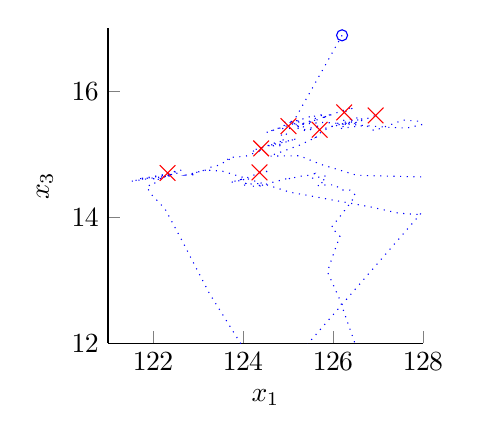
\begin{tikzpicture}

\begin{axis}[%
width=4cm,
height=4cm,
scale only axis,
xmin=121,
xmax=128,
xlabel={$x_1$},
ymin=12,
ymax=17,
ylabel={$x_3$},
axis x line*=bottom,
axis y line*=left
]
\addplot [
color=blue,
dotted,
forget plot
]
table[row sep=crcr]{
133.35681987922 10.8841024888732\\
135.782024142063 18.3350084656896\\
135.57509347932 18.9040537944205\\
134.866483579293 20.3805414313985\\
134.476333455592 20.9618193556903\\
134.091538927312 21.5766940301034\\
134.011568443763 21.8255217930903\\
134.046057425386 21.8467627620992\\
134.091316154945 21.7950728965056\\
134.045091685323 21.7952002659453\\
134.206612301894 21.7975551420049\\
134.208853749002 21.7890653106618\\
134.189853293825 21.8032130333547\\
134.323186650354 21.797468353246\\
134.41293316264 21.7919281843479\\
134.390212651898 21.7950146669832\\
134.390667355101 21.8493839152079\\
134.499953805048 21.7833518952136\\
134.341012902163 21.7976524908878\\
134.308548350366 21.805836847949\\
134.31528742678 21.8045136108208\\
134.397781962528 21.7769867043344\\
134.371917940411 21.7772624288922\\
134.333783609591 21.7982576289909\\
134.24421436661 21.8225875921588\\
134.321290163699 21.797923490581\\
134.212270722605 21.8327027810045\\
134.174559958789 21.8272129207476\\
134.054378284642 21.8632364622274\\
133.946266826988 21.8804216426222\\
133.99267217835 21.8648495050247\\
134.00314288986 21.8697386406148\\
133.982128285993 21.877314279164\\
};
\addplot [
color=blue,
only marks,
mark=o,
mark options={solid},
forget plot
]
table[row sep=crcr]{
133.35681987922 10.8841024888732\\
};
\addplot [
color=red,
mark size=4.0pt,
only marks,
mark=x,
mark options={solid},
forget plot
]
table[row sep=crcr]{
133.982128285993 21.877314279164\\
};
\addplot [
color=blue,
dotted,
forget plot
]
table[row sep=crcr]{
133.160008391131 13.5599911393441\\
133.449478766983 19.8689745820507\\
133.144489919092 20.3918948351497\\
132.364704831709 21.5901002355652\\
131.88591675204 22.2089562770786\\
131.565103515987 22.6720108506258\\
131.473240449167 22.776181723731\\
131.487787146732 22.7572250981471\\
131.33431173094 22.858999452293\\
131.323181246468 22.8313881431084\\
131.133378072109 22.9458953427952\\
131.060462546266 23.0103746432949\\
131.097188610767 22.9574679341916\\
131.216578501029 22.9040673756242\\
130.871263564287 23.0665443901768\\
130.871172238185 23.0554893446539\\
130.561373722662 23.2235004667535\\
130.450298804616 23.2910943703734\\
130.370287591378 23.3416342276114\\
130.340050355482 23.3692979594318\\
130.708392081269 23.1668104922262\\
130.67160701893 23.1819054281433\\
130.874541146985 23.0790300119654\\
131.02699448289 22.9934901071988\\
130.859632276542 23.0945539005886\\
130.834980363136 23.1085937605101\\
130.788531822455 23.1134347318513\\
130.846654509879 23.0652256154693\\
131.127305194158 22.9225513261913\\
131.122453839847 22.9280920221196\\
131.08790554646 22.9583714926942\\
131.248971058486 22.8990583321476\\
131.526187511036 22.7605761442911\\
};
\addplot [
color=blue,
only marks,
mark=o,
mark options={solid},
forget plot
]
table[row sep=crcr]{
133.160008391131 13.5599911393441\\
};
\addplot [
color=red,
mark size=4.0pt,
only marks,
mark=x,
mark options={solid},
forget plot
]
table[row sep=crcr]{
131.526187511036 22.7605761442911\\
};
\addplot [
color=blue,
dotted,
forget plot
]
table[row sep=crcr]{
143.20680332871 8.87687295689003\\
135.235244071681 16.8942053308934\\
134.89533494454 17.3502081514563\\
133.461027592108 19.2169488849485\\
132.757542181983 20.043874841765\\
131.737433220973 21.1523979585777\\
131.123504220912 21.8713555033806\\
130.478005816325 22.6177090796799\\
130.121155117354 23.0760012827078\\
129.807216421995 23.3947309765173\\
129.731107721037 23.4744600108122\\
129.686099920016 23.5118463446882\\
129.352139701215 23.780759494488\\
129.560227576531 23.6765450025851\\
129.438874234221 23.7571945412585\\
129.631355382773 23.6481330780928\\
129.759194965519 23.5669602246332\\
129.740953871895 23.599872220905\\
129.445131653716 23.7815525081069\\
129.593419245559 23.690131144999\\
129.551143201341 23.6958136563596\\
129.533297350729 23.7110027215062\\
129.597315530746 23.7049162850313\\
129.726894211752 23.6204285351807\\
129.476946683294 23.7589980080704\\
129.566952606352 23.7036185684701\\
129.309679865832 23.8719424456827\\
129.452117480558 23.7863214380598\\
129.753290545194 23.6162720480936\\
129.477856882648 23.7891041246758\\
129.740396563773 23.6378601631169\\
129.746921159353 23.6343692145659\\
129.710757791667 23.657702360106\\
129.802166457792 23.6017264123619\\
129.455922313599 23.7938296866919\\
129.753270667566 23.6158032417238\\
129.845886301514 23.5600569233789\\
129.862477135031 23.5376396790938\\
129.851698022462 23.5455606590315\\
129.982389558789 23.4676580593803\\
129.574162321503 23.7007953627285\\
129.668567326594 23.6281745293068\\
129.719376822335 23.6035288274345\\
129.845726595208 23.5280551639142\\
130.030052518341 23.4177074415315\\
130.109846805455 23.3867473274397\\
130.025761923365 23.440825106366\\
130.073001675758 23.4217264366974\\
};
\addplot [
color=blue,
only marks,
mark=o,
mark options={solid},
forget plot
]
table[row sep=crcr]{
143.20680332871 8.87687295689003\\
};
\addplot [
color=red,
mark size=4.0pt,
only marks,
mark=x,
mark options={solid},
forget plot
]
table[row sep=crcr]{
130.073001675758 23.4217264366974\\
};
\addplot [
color=blue,
dotted,
forget plot
]
table[row sep=crcr]{
131.052986240617 5.09058887006587\\
136.769132569683 16.1638796328243\\
136.694000052856 16.6761688458786\\
136.097046730623 18.7971064680617\\
135.706429749464 19.6921919077987\\
135.400498915658 20.5574042513649\\
135.32303260151 20.7276291613816\\
135.357969775363 20.6558232947679\\
135.316928023246 20.6527530898506\\
135.559149975229 20.7294677636766\\
135.587451283836 20.7225428231096\\
135.762887042213 20.8438896048915\\
135.689812060863 20.72580731452\\
135.796881801555 20.8171013331091\\
135.831010742575 20.8044111592631\\
135.750775428774 20.7112982299106\\
135.815948330453 20.7561500983917\\
135.887402856826 20.8431893637085\\
135.880422234357 20.8400105264865\\
135.8755369688 20.8124888907155\\
135.854779381398 20.7859626890821\\
135.996580396927 20.9113080961945\\
136.11193723885 20.9934972728516\\
136.131793538172 21.0607612013205\\
136.129978721014 21.0530882727393\\
136.143323684285 21.1059518900153\\
136.288111202676 21.2337466360209\\
136.260889890625 21.2083264386561\\
136.35406875641 21.2204034838224\\
};
\addplot [
color=blue,
only marks,
mark=o,
mark options={solid},
forget plot
]
table[row sep=crcr]{
131.052986240617 5.09058887006587\\
};
\addplot [
color=red,
mark size=4.0pt,
only marks,
mark=x,
mark options={solid},
forget plot
]
table[row sep=crcr]{
136.35406875641 21.2204034838224\\
};
\addplot [
color=blue,
dotted,
forget plot
]
table[row sep=crcr]{
148.512736993562 15.3904813154739\\
140.500433916728 17.5613370473093\\
139.92579519574 17.8780954442517\\
138.249125006672 18.5282784339577\\
137.314253307051 18.8812897469503\\
136.310255332791 19.1430933148239\\
135.694128029056 19.3806466948105\\
135.320413388251 19.3819861378952\\
135.061439131878 19.3852739243448\\
134.906495317052 19.3808254231458\\
134.830843952877 19.3349745761559\\
134.80233261858 19.3446011072985\\
134.753359274065 19.3325483117418\\
134.667791938518 19.2865853424925\\
134.707674474782 19.2817435931247\\
134.660048864074 19.2728024024862\\
134.746380784734 19.3724015432573\\
134.6654023789 19.3120599231126\\
134.720271853585 19.3811393822452\\
134.697544457098 19.36905980241\\
134.81420604901 19.4693537524632\\
134.869047374551 19.543692818667\\
134.921441029399 19.6019646596035\\
134.958778070813 19.6267235640126\\
134.901137915199 19.5959531543688\\
134.830430553051 19.5590164093309\\
134.839945086601 19.5622972385292\\
134.93005568732 19.6496359310434\\
134.950430058007 19.6805538884448\\
135.069771847784 19.7792175796452\\
135.030471258535 19.7673642390745\\
134.991549631385 19.7442368655288\\
135.071814537628 19.8011763595663\\
135.005121289065 19.7366971129458\\
135.020442474514 19.7540736447335\\
135.01023319416 19.7633559784229\\
134.951955082193 19.7085516327754\\
135.031751510473 19.7781527022615\\
134.987025266896 19.7085429097382\\
134.851738416172 19.634791503933\\
134.909492449524 19.6772915548511\\
134.801114511916 19.6345258691261\\
134.759692595587 19.6074880519801\\
134.808104223171 19.6599196407939\\
134.790038050889 19.6587378219124\\
134.647765817105 19.5394136092559\\
134.615777077518 19.5135423507279\\
};
\addplot [
color=blue,
only marks,
mark=o,
mark options={solid},
forget plot
]
table[row sep=crcr]{
148.512736993562 15.3904813154739\\
};
\addplot [
color=red,
mark size=4.0pt,
only marks,
mark=x,
mark options={solid},
forget plot
]
table[row sep=crcr]{
134.615777077518 19.5135423507279\\
};
\addplot [
color=blue,
dotted,
forget plot
]
table[row sep=crcr]{
151.906798640258 7.1052098635708\\
141.792448570141 14.8015860974617\\
141.370193745236 15.348990661548\\
139.86632956315 17.3437027494923\\
139.049544660557 18.3996882908444\\
138.158057453392 19.4358215311757\\
137.485173711019 20.3218233114798\\
137.001122606493 20.9254627840571\\
136.787748540759 21.2676670198431\\
136.697595043522 21.3955434701856\\
136.616436511598 21.5069436790044\\
136.598317162897 21.5873306155225\\
136.50364693295 21.6414157896254\\
136.47192288021 21.6681650058447\\
136.494460812277 21.6652934709388\\
136.527777594046 21.6549945430499\\
136.47156757339 21.6980182700856\\
136.464396730428 21.6775970106855\\
136.434112987683 21.7010709013654\\
136.464143776187 21.714154664906\\
136.526205143631 21.6803639958699\\
136.523300023519 21.6545268100202\\
136.520027663356 21.6645999521664\\
};
\addplot [
color=blue,
only marks,
mark=o,
mark options={solid},
forget plot
]
table[row sep=crcr]{
151.906798640258 7.1052098635708\\
};
\addplot [
color=red,
mark size=4.0pt,
only marks,
mark=x,
mark options={solid},
forget plot
]
table[row sep=crcr]{
136.520027663356 21.6645999521664\\
};
\addplot [
color=blue,
dotted,
forget plot
]
table[row sep=crcr]{
140.053745570725 3.34201234577398\\
139.648301731597 12.1961189619945\\
139.439042587461 12.9061466922868\\
138.653069109721 15.0602749273854\\
138.098197728534 16.2925025252176\\
137.543939757003 17.6273565665581\\
137.045888906914 18.7394245065451\\
136.677889705923 19.5108382030201\\
136.580226236197 19.9713629174016\\
136.511112448775 20.2291080125046\\
136.410152764339 20.4685400935543\\
136.389165397134 20.6025195416407\\
136.351841319653 20.7356746782527\\
136.242919572448 20.8360360835318\\
136.238857488331 20.8962149349967\\
136.244684825996 20.9323392363758\\
136.301268803329 21.0114999102428\\
136.300428659625 21.048890344061\\
136.232379482981 21.0815525015906\\
136.189160840509 21.1055712988425\\
136.143675205944 21.1088610148751\\
136.078003343325 21.1225777644543\\
135.979397145413 21.1398009093369\\
135.990689285694 21.1347020070727\\
135.991783046264 21.1542091193352\\
136.123462793211 21.1789129104874\\
136.113587286424 21.1923572776004\\
136.206076349176 21.1860713247546\\
136.174264595805 21.1953041135426\\
136.215674415091 21.2176812929882\\
136.187049103282 21.2671269388858\\
136.112195770605 21.2382201386713\\
136.068118011354 21.2338689465609\\
136.050384522379 21.257017245011\\
136.04356471359 21.241183988439\\
136.019542857237 21.2542025120454\\
135.941229140592 21.2758535630938\\
135.946870026278 21.2732494873411\\
135.995495141977 21.259227057612\\
136.009354813969 21.2519205486615\\
136.02148524263 21.2566621886669\\
135.971638231243 21.279794849391\\
135.975678604238 21.2799054626262\\
136.045596637463 21.2793591449809\\
136.066271064499 21.2839893504678\\
136.094445911949 21.30605764635\\
};
\addplot [
color=blue,
only marks,
mark=o,
mark options={solid},
forget plot
]
table[row sep=crcr]{
140.053745570725 3.34201234577398\\
};
\addplot [
color=red,
mark size=4.0pt,
only marks,
mark=x,
mark options={solid},
forget plot
]
table[row sep=crcr]{
136.094445911949 21.30605764635\\
};
\addplot [
color=blue,
dotted,
forget plot
]
table[row sep=crcr]{
144.440883612646 13.6073336481048\\
139.865243333028 19.3894057294508\\
139.434761426767 19.8178949004829\\
138.103841814098 20.890030036249\\
137.473673969363 21.3202704099808\\
136.853006498686 21.6691106330355\\
136.686068225218 21.7518034426351\\
136.619517602502 21.7781275158887\\
136.608903084677 21.776488496718\\
136.563881194097 21.7995471463482\\
136.533852694694 21.8293023811708\\
136.564184181348 21.7769285323554\\
136.572987891828 21.7492297320801\\
136.53363723059 21.8110487031099\\
136.540534340263 21.7780875718528\\
136.497214158823 21.8134802621056\\
136.519342534158 21.8111748295313\\
136.485119570677 21.8442489958538\\
136.480152614308 21.8396991256253\\
136.478495616728 21.8270471584371\\
136.464180544121 21.8306682965317\\
136.48171878492 21.8090712853838\\
136.483385539617 21.7980033663115\\
136.471541970794 21.8174251148982\\
136.474741695899 21.8133223326696\\
136.48716658592 21.7899455335536\\
136.486688300291 21.7870847573493\\
136.491387334896 21.7924566822186\\
136.498449699438 21.752001196139\\
136.498730571158 21.7435827523571\\
136.497212700815 21.7358618088181\\
136.47610881871 21.7592174174864\\
136.484558395975 21.7543924732638\\
136.470812492999 21.764748330727\\
136.453737847106 21.7496480226846\\
136.455964127174 21.7474333786533\\
136.446315914005 21.7282718542757\\
136.465480278569 21.7209612800237\\
136.39550114631 21.7383975057532\\
136.346372038353 21.7404196363215\\
136.321318362308 21.7385056845697\\
};
\addplot [
color=blue,
only marks,
mark=o,
mark options={solid},
forget plot
]
table[row sep=crcr]{
144.440883612646 13.6073336481048\\
};
\addplot [
color=red,
mark size=4.0pt,
only marks,
mark=x,
mark options={solid},
forget plot
]
table[row sep=crcr]{
136.321318362308 21.7385056845697\\
};
\addplot [
color=blue,
dotted,
forget plot
]
table[row sep=crcr]{
138.707108444427 14.4605653155275\\
137.517068901658 19.1419341399151\\
137.148861970189 19.748119939597\\
136.377164325071 20.8444598534001\\
136.026095771031 21.285889472532\\
136.079464452594 21.4586860822816\\
136.110883568672 21.5647536299053\\
136.198330372934 21.6238438845911\\
136.284820495282 21.6037126792987\\
136.325039481777 21.5728570294027\\
136.343808512852 21.5472742321351\\
136.337308666711 21.5024297102643\\
136.383006526229 21.4867193883965\\
136.366991103322 21.5231687633102\\
136.410746459891 21.5542183289499\\
136.463686306669 21.6240580999763\\
136.439683306895 21.6286737028111\\
136.445821045678 21.6332971446531\\
136.429330691866 21.6394463126636\\
136.448110355015 21.6820382011676\\
136.463694291238 21.6786341566361\\
136.493327906379 21.6621096374548\\
136.495176053848 21.6586897185579\\
};
\addplot [
color=blue,
only marks,
mark=o,
mark options={solid},
forget plot
]
table[row sep=crcr]{
138.707108444427 14.4605653155275\\
};
\addplot [
color=red,
mark size=4.0pt,
only marks,
mark=x,
mark options={solid},
forget plot
]
table[row sep=crcr]{
136.495176053848 21.6586897185579\\
};
\addplot [
color=blue,
dotted,
forget plot
]
table[row sep=crcr]{
148.493253261674 4.18802879860039\\
141.994019826264 15.5299046904358\\
141.637476116622 16.0368971549345\\
140.183942233046 17.9042296711462\\
139.381909324717 18.796582053405\\
138.43652302229 19.8003825159516\\
137.697652944704 20.4875898154129\\
137.217324762828 20.9039474881068\\
136.685517902574 21.383251076664\\
136.684458549664 21.4500687415276\\
136.659732054973 21.466475187437\\
136.647795473594 21.4781685941911\\
136.654117146467 21.4602061781976\\
136.676924144314 21.4723825939268\\
136.712215797662 21.4694454327953\\
136.710591078135 21.4606920177547\\
136.720084962626 21.4261440676166\\
136.717496924846 21.4328624772352\\
136.710701621247 21.4325526175699\\
136.708726367165 21.4663812227815\\
136.684766582361 21.5035262962023\\
136.65353164082 21.5563044134676\\
};
\addplot [
color=blue,
only marks,
mark=o,
mark options={solid},
forget plot
]
table[row sep=crcr]{
148.493253261674 4.18802879860039\\
};
\addplot [
color=red,
mark size=4.0pt,
only marks,
mark=x,
mark options={solid},
forget plot
]
table[row sep=crcr]{
136.65353164082 21.5563044134676\\
};
\addplot [
color=blue,
dotted,
forget plot
]
table[row sep=crcr]{
147.904353571163 17.6587971110626\\
140.001203228409 20.1035596260969\\
139.617804887346 20.3610145189852\\
138.114569636093 21.2681335139423\\
137.529218078131 21.5166814207351\\
136.887897915007 21.6960838995029\\
136.690523095953 21.7180316997077\\
136.656648097893 21.6719488720284\\
136.624340603811 21.6651891133315\\
136.586000549347 21.6929283897238\\
136.625484973734 21.6609667493241\\
136.660762306705 21.6576671280954\\
136.665370446876 21.6543733843069\\
136.633480062327 21.7060710378836\\
136.577467834127 21.7475832412873\\
136.580631238645 21.7568170209064\\
136.55320763743 21.7550056515172\\
136.539410943685 21.7738653805241\\
136.573616577576 21.7408455051924\\
136.581983644356 21.7424179027951\\
136.611154015802 21.750472930963\\
136.615048398587 21.7514393561894\\
136.615654235039 21.7350284818479\\
136.624881435709 21.702688403039\\
};
\addplot [
color=blue,
only marks,
mark=o,
mark options={solid},
forget plot
]
table[row sep=crcr]{
147.904353571163 17.6587971110626\\
};
\addplot [
color=red,
mark size=4.0pt,
only marks,
mark=x,
mark options={solid},
forget plot
]
table[row sep=crcr]{
136.624881435709 21.702688403039\\
};
\addplot [
color=blue,
dotted,
forget plot
]
table[row sep=crcr]{
146.222126709961 12.2775971359114\\
140.650439788368 17.825266497131\\
140.2142510488 18.3094958067393\\
138.874805961801 19.6457370572403\\
138.113812151319 20.3065718615453\\
137.438497358016 20.9470530301093\\
136.981739210715 21.2469066758009\\
136.810990676361 21.3773612223516\\
136.759345875462 21.4174371036749\\
136.692402390356 21.4593855274275\\
136.710059797642 21.4771368737123\\
136.70548571576 21.4763064037857\\
136.693194022673 21.4970977261304\\
136.676637140397 21.5054746041669\\
136.693797172392 21.4927099778997\\
136.681031705252 21.5086383072555\\
136.685748974635 21.4761687244504\\
136.673705307606 21.4846858379119\\
136.642715452646 21.5032978073848\\
136.643742062452 21.5056036778593\\
136.611220797468 21.5384267983231\\
136.617059565105 21.5146404814941\\
136.614881035475 21.4776406907969\\
136.604090779159 21.4618127981378\\
};
\addplot [
color=blue,
only marks,
mark=o,
mark options={solid},
forget plot
]
table[row sep=crcr]{
146.222126709961 12.2775971359114\\
};
\addplot [
color=red,
mark size=4.0pt,
only marks,
mark=x,
mark options={solid},
forget plot
]
table[row sep=crcr]{
136.604090779159 21.4618127981378\\
};
\addplot [
color=blue,
dotted,
forget plot
]
table[row sep=crcr]{
152.957003818275 13.3843009194259\\
141.913485401573 17.4931451610916\\
141.519785943697 17.8618965363057\\
139.791270232482 19.1734176132841\\
138.901856810221 19.8454006000655\\
137.993455393843 20.4730504218173\\
137.388827439686 20.8924467278293\\
136.929410772471 21.2018287131847\\
136.790671592794 21.2865955918506\\
136.655653508561 21.335617864279\\
136.577568348169 21.3627343646783\\
136.469693522774 21.3161879363619\\
136.44831768498 21.2881674941332\\
136.442764560463 21.3056098863052\\
136.453433166087 21.3327806311238\\
136.462179521449 21.3463941523822\\
136.43759363627 21.3117935019599\\
136.454086461349 21.2465554669397\\
136.484508158269 21.2080153025134\\
136.466849591824 21.1943271204253\\
136.502093187085 21.268826634524\\
136.478388749938 21.3021393079629\\
136.451974341364 21.2918104982775\\
136.450679592018 21.2799103400538\\
136.446160738944 21.2578238416742\\
136.503297880298 21.317601891336\\
136.475111998762 21.3008447866059\\
136.485971870414 21.296664768155\\
136.448828896093 21.2520226577643\\
136.466334345173 21.2686523721208\\
136.453331558674 21.253255166117\\
};
\addplot [
color=blue,
only marks,
mark=o,
mark options={solid},
forget plot
]
table[row sep=crcr]{
152.957003818275 13.3843009194259\\
};
\addplot [
color=red,
mark size=4.0pt,
only marks,
mark=x,
mark options={solid},
forget plot
]
table[row sep=crcr]{
136.453331558674 21.253255166117\\
};
\addplot [
color=blue,
dotted,
forget plot
]
table[row sep=crcr]{
133.140938029048 0.423893685163373\\
134.85650994314 10.3596674903798\\
134.611210276952 10.9667925321144\\
133.553988089068 13.0808892308164\\
132.740453313 14.2068567999667\\
131.855337158509 15.2491814798711\\
131.27608437178 15.9905962092909\\
130.965584264481 16.4650453323197\\
130.877090659993 16.6620525163536\\
130.777303306117 16.7217290436228\\
130.571473593332 16.7586161311988\\
130.651713433972 16.8851440772025\\
131.044966848204 17.0853458980455\\
130.976770004314 17.0964704416748\\
131.030585586291 17.1790487544809\\
131.094415895654 17.2043805533386\\
131.224670238508 17.2362294798439\\
131.04389121119 17.1730698368538\\
131.178837313938 17.2493819996083\\
131.603562240126 17.4589899618486\\
131.380730680203 17.3520201449807\\
131.237753475092 17.2545119894278\\
131.264719412586 17.293498128399\\
131.186778838468 17.2838367132672\\
131.452038038645 17.4215437090147\\
};
\addplot [
color=blue,
only marks,
mark=o,
mark options={solid},
forget plot
]
table[row sep=crcr]{
133.140938029048 0.423893685163373\\
};
\addplot [
color=red,
mark size=4.0pt,
only marks,
mark=x,
mark options={solid},
forget plot
]
table[row sep=crcr]{
131.452038038645 17.4215437090147\\
};
\addplot [
color=blue,
dotted,
forget plot
]
table[row sep=crcr]{
141.450900185129 7.99655600290338\\
133.323905922782 14.4434379269866\\
132.940171118768 14.9370316399587\\
131.542364478063 16.4268309889025\\
131.095362273191 17.007886717109\\
130.912656090578 17.4009719079748\\
131.091362659034 17.5854619511773\\
131.037074035237 17.555395224643\\
131.007969265499 17.517275240159\\
131.036213033332 17.4829570919446\\
131.218166252208 17.4454788366715\\
130.90125311612 17.2926071104624\\
130.777006287422 17.2177147441736\\
130.90344730211 17.2455728255357\\
131.023107192272 17.3436053863652\\
130.753808294442 17.1925947620499\\
130.750654907173 17.187101686516\\
130.56614374019 17.1209585735607\\
130.054913317321 16.77832229734\\
130.671479358298 17.0608999578385\\
};
\addplot [
color=blue,
only marks,
mark=o,
mark options={solid},
forget plot
]
table[row sep=crcr]{
141.450900185129 7.99655600290338\\
};
\addplot [
color=red,
mark size=4.0pt,
only marks,
mark=x,
mark options={solid},
forget plot
]
table[row sep=crcr]{
130.671479358298 17.0608999578385\\
};
\addplot [
color=blue,
dotted,
forget plot
]
table[row sep=crcr]{
134.884569833816 16.6145948545627\\
127.637699556941 15.4147925596201\\
127.22553210911 15.4261758192467\\
125.797937962182 15.5052159327534\\
125.152871592007 15.4697606538607\\
125.181124012828 15.4211222871642\\
125.422421312128 15.3642584260906\\
125.478621683467 15.3839951131144\\
125.716392843703 15.455812121312\\
125.308867018717 15.3793356556685\\
125.352621036443 15.4496845548011\\
125.151265203294 15.4310453536618\\
125.369012206007 15.4976280009695\\
125.588287894732 15.5228331696302\\
125.608384566315 15.5426608879474\\
125.556301859876 15.5281570259519\\
125.480801721375 15.5047495118433\\
125.680451089546 15.5551021683341\\
125.945775786211 15.6295530512955\\
125.754594031834 15.5730689870945\\
126.405587904426 15.7416229915988\\
126.463456856347 15.740425987963\\
126.248465739532 15.6639039377817\\
};
\addplot [
color=blue,
only marks,
mark=o,
mark options={solid},
forget plot
]
table[row sep=crcr]{
134.884569833816 16.6145948545627\\
};
\addplot [
color=red,
mark size=4.0pt,
only marks,
mark=x,
mark options={solid},
forget plot
]
table[row sep=crcr]{
126.248465739532 15.6639039377817\\
};
\addplot [
color=blue,
dotted,
forget plot
]
table[row sep=crcr]{
138.096450518276 17.0984626757134\\
128.905828748532 14.6111971446991\\
128.388599021106 14.6316423648525\\
126.529945953373 14.664486227254\\
125.731210557318 14.8377176299928\\
125.252530635592 14.9754386327099\\
124.5911904149 14.9692649615023\\
125.246980796857 15.1404781426845\\
125.641441859512 15.2746498761538\\
125.621516439579 15.2701288099438\\
125.748127080504 15.3599063430865\\
126.251718962182 15.5423341696421\\
126.542831818605 15.5754945000444\\
126.212055468718 15.4617923264901\\
126.66297158896 15.570477755611\\
126.515744807969 15.5057140727406\\
126.50667100614 15.4996760701592\\
126.940309856304 15.6122887913648\\
126.947282491398 15.6154597671475\\
};
\addplot [
color=blue,
only marks,
mark=o,
mark options={solid},
forget plot
]
table[row sep=crcr]{
138.096450518276 17.0984626757134\\
};
\addplot [
color=red,
mark size=4.0pt,
only marks,
mark=x,
mark options={solid},
forget plot
]
table[row sep=crcr]{
126.947282491398 15.6154597671475\\
};
\addplot [
color=blue,
dotted,
forget plot
]
table[row sep=crcr]{
139.136463682346 -12.4916162733161\\
132.818916305362 1.3645160205038\\
132.459274333766 2.08077885031918\\
131.030246031888 4.72107155500598\\
130.042996654526 6.22608774970005\\
128.96468876213 7.92596053484299\\
127.987401728797 9.53673836287025\\
127.125513435002 10.9419784219689\\
126.477210359182 12.0188527768657\\
126.135222404201 12.716997135028\\
125.876181550275 13.1333046431272\\
126.040496284 13.4800208021185\\
126.153563769412 13.6946637666746\\
125.965674828728 13.8396768989045\\
126.217710156235 14.0680477035335\\
126.408222106495 14.246565686453\\
126.494474765105 14.3511279476418\\
126.37809765002 14.4296839955338\\
126.181815131684 14.4321313728911\\
126.04348073492 14.5138137467427\\
125.80298640105 14.5115284868024\\
125.650634539718 14.4998789455873\\
125.790383704201 14.5649671984939\\
125.744839064869 14.5721474001727\\
125.868115567101 14.6249032026908\\
125.832877502641 14.6498708461342\\
125.781687666349 14.6625100822209\\
125.738044673691 14.6454079065665\\
125.609289622407 14.6223883992046\\
125.569345626496 14.6080300173855\\
125.518541697621 14.6379168593498\\
125.588632963195 14.690254136804\\
125.38019525427 14.6524050434246\\
125.285776663335 14.6524308619897\\
125.019597124499 14.6070479730181\\
125.058950381958 14.6274688435642\\
124.624305769652 14.5468347730864\\
124.335318593778 14.4863880401174\\
124.461140169293 14.5159501679746\\
124.463087613012 14.5241469085168\\
124.348815481575 14.5022392436001\\
124.2217555071 14.4907092312328\\
124.225741767559 14.4909066413904\\
124.344523219871 14.533041171703\\
124.195133988203 14.5296777018943\\
123.983287439993 14.5022186673524\\
124.061177267123 14.5351939267302\\
124.003972955619 14.5556102869982\\
123.975185464376 14.5677050087832\\
124.002325059047 14.5907160404878\\
124.047144645911 14.6108392742034\\
123.875185196989 14.5871450880881\\
123.929203895127 14.580255288868\\
123.719050845225 14.5524672147071\\
124.040412601458 14.6167385738871\\
124.040563353826 14.6167162498932\\
124.16870087752 14.644643856689\\
124.195680913872 14.6544349562844\\
124.270908721369 14.6763630449104\\
124.382217015852 14.6952209263473\\
124.596883356891 14.7368302599982\\
124.469274076304 14.7218357169521\\
124.366356756327 14.7109040797072\\
};
\addplot [
color=blue,
only marks,
mark=o,
mark options={solid},
forget plot
]
table[row sep=crcr]{
139.136463682346 -12.4916162733161\\
};
\addplot [
color=red,
mark size=4.0pt,
only marks,
mark=x,
mark options={solid},
forget plot
]
table[row sep=crcr]{
124.366356756327 14.7109040797072\\
};
\addplot [
color=blue,
dotted,
forget plot
]
table[row sep=crcr]{
126.201955654672 16.8871518357841\\
124.805309616399 15.1163425675002\\
124.888692385015 15.4269167176387\\
124.935682459079 15.5131214625906\\
125.243272288487 15.5310297016916\\
125.337983342316 15.4766490589948\\
125.806449862638 15.6353236124596\\
125.524560862432 15.5942654078857\\
125.531277496672 15.6069173937454\\
125.303502248126 15.5531503469429\\
125.089903179904 15.5156135334585\\
124.762372473723 15.404748295423\\
124.520257859857 15.3452496276435\\
125.262855090882 15.515902176238\\
125.010081365321 15.4453112565398\\
};
\addplot [
color=blue,
only marks,
mark=o,
mark options={solid},
forget plot
]
table[row sep=crcr]{
126.201955654672 16.8871518357841\\
};
\addplot [
color=red,
mark size=4.0pt,
only marks,
mark=x,
mark options={solid},
forget plot
]
table[row sep=crcr]{
125.010081365321 15.4453112565398\\
};
\addplot [
color=blue,
dotted,
forget plot
]
table[row sep=crcr]{
139.487752632874 20.4466722484334\\
132.720828337788 15.6945328351423\\
132.016282059625 15.5177779797163\\
130.034982554739 15.218370256307\\
128.986428004355 15.3005496057855\\
128.231933120526 15.5053591745869\\
127.564726543768 15.5422081337858\\
126.911737910466 15.3730239873954\\
126.740639018516 15.4568160899308\\
126.454429051817 15.4357254132262\\
126.138985981571 15.4042460995135\\
126.316441404773 15.476764509282\\
126.425894693376 15.5175648502347\\
126.198983065469 15.470126204589\\
126.287162342371 15.5132773599795\\
126.04017891141 15.4412774441459\\
126.103166639486 15.4627258035288\\
125.703840514416 15.3883462412191\\
};
\addplot [
color=blue,
only marks,
mark=o,
mark options={solid},
forget plot
]
table[row sep=crcr]{
139.487752632874 20.4466722484334\\
};
\addplot [
color=red,
mark size=4.0pt,
only marks,
mark=x,
mark options={solid},
forget plot
]
table[row sep=crcr]{
125.703840514416 15.3883462412191\\
};
\addplot [
color=blue,
dotted,
forget plot
]
table[row sep=crcr]{
127.514736695982 3.21104152442964\\
122.27756685408 9.92731881462103\\
121.858537600854 10.6274903851992\\
120.741153925957 12.2505616500995\\
119.892696640722 13.2052078251658\\
119.800712342504 13.8701931991109\\
119.658253608467 14.1523911830742\\
119.979217970126 14.2971827676232\\
119.802692560044 14.3500350340281\\
120.233507086327 14.4116044317753\\
119.836174272696 14.369928581975\\
120.029801822183 14.3980480633381\\
120.448516167323 14.4241840428704\\
120.220987915672 14.4187024347217\\
120.386158066379 14.4398492449307\\
120.524024680298 14.4864748059584\\
120.175754696185 14.4669282402774\\
120.195214632258 14.5133814808028\\
119.757773007379 14.4982472843014\\
120.195023215733 14.5048450797893\\
120.000223759769 14.5134537919327\\
119.823045061226 14.4942115604085\\
};
\addplot [
color=blue,
only marks,
mark=o,
mark options={solid},
forget plot
]
table[row sep=crcr]{
127.514736695982 3.21104152442964\\
};
\addplot [
color=red,
mark size=4.0pt,
only marks,
mark=x,
mark options={solid},
forget plot
]
table[row sep=crcr]{
119.823045061226 14.4942115604085\\
};
\addplot [
color=blue,
dotted,
forget plot
]
table[row sep=crcr]{
138.965966654712 17.8272866905193\\
134.703261591021 18.9926947218371\\
134.150494574926 19.116644062052\\
133.162737149118 18.9071589049104\\
132.600917496034 18.6811264779745\\
132.511561208206 18.6552778955655\\
132.386648229104 18.4745014861552\\
132.486968198696 18.4819541542558\\
132.278556192056 18.3799110142602\\
132.161768736893 18.3418418983441\\
131.986511576826 18.2104915051794\\
132.267016962701 18.2535036307424\\
132.158705269825 18.2102056026127\\
132.157696558329 18.1856990595235\\
132.460593458563 18.3460184271584\\
132.147182891309 18.1511203353575\\
132.411336713901 18.2894444711274\\
132.304191037143 18.2296656589066\\
132.408811739996 18.2935422978808\\
132.73474355817 18.5009204866406\\
132.620808615886 18.4796767633624\\
132.603273751042 18.4669163376964\\
132.604470009486 18.4700402393568\\
};
\addplot [
color=blue,
only marks,
mark=o,
mark options={solid},
forget plot
]
table[row sep=crcr]{
138.965966654712 17.8272866905193\\
};
\addplot [
color=red,
mark size=4.0pt,
only marks,
mark=x,
mark options={solid},
forget plot
]
table[row sep=crcr]{
132.604470009486 18.4700402393568\\
};
\addplot [
color=blue,
dotted,
forget plot
]
table[row sep=crcr]{
151.000417341045 16.9445999516813\\
142.835793365477 18.9714963972081\\
142.364131625273 19.2434223861179\\
140.62243678046 20.0985581180154\\
139.7499719746 20.547314433434\\
138.77126735104 20.9190397571417\\
138.064991925236 21.2060025987591\\
137.555643121928 21.3864154461138\\
137.335692873603 21.5066281982213\\
137.190992107652 21.5254686838428\\
137.076026931938 21.557882292215\\
137.057906130256 21.5621158073849\\
137.052582391988 21.597099296817\\
136.977001217023 21.6178077551825\\
136.908183330153 21.6310724377815\\
136.859567327311 21.6146793240278\\
136.825527569458 21.6317390382884\\
136.807997750015 21.6204156938469\\
136.791054575446 21.6183233675191\\
136.780042266649 21.6190903288472\\
136.771877600044 21.6531366352989\\
136.754086687226 21.668741937674\\
136.725414606464 21.6858091223226\\
136.703601982947 21.7192934271523\\
136.674090079907 21.7335217821081\\
136.710538264025 21.7130879299658\\
136.72289486174 21.7239529141499\\
136.695317698861 21.7325342178587\\
136.681042364883 21.74655918358\\
136.643912580125 21.7653811088259\\
136.652394959041 21.7498152816504\\
136.629967954167 21.7258508093192\\
136.631719711888 21.6968085508605\\
136.644045958998 21.6962986733397\\
136.619877408237 21.7103738283351\\
136.610632390514 21.6932999285671\\
136.605085480613 21.6950940992401\\
136.597019176578 21.7037801916829\\
};
\addplot [
color=blue,
only marks,
mark=o,
mark options={solid},
forget plot
]
table[row sep=crcr]{
151.000417341045 16.9445999516813\\
};
\addplot [
color=red,
mark size=4.0pt,
only marks,
mark=x,
mark options={solid},
forget plot
]
table[row sep=crcr]{
136.597019176578 21.7037801916829\\
};
\addplot [
color=blue,
dotted,
forget plot
]
table[row sep=crcr]{
139.986618811135 25.0264409762746\\
135.597546539431 20.1428903009167\\
135.003882891517 19.6132550062905\\
133.609326688654 18.6490499068748\\
132.785649807011 18.2899128820377\\
132.555015925189 18.0337996369595\\
132.498373674673 18.0903054026251\\
132.567108505515 18.2031226145939\\
132.319046461443 18.0673253540282\\
132.085614728701 17.8705393877919\\
132.07009663136 17.8946783752456\\
132.067454957777 17.9016259931772\\
132.000777606419 17.8865674978161\\
131.893353413213 17.8319889228815\\
131.746839130417 17.7588123080992\\
131.618128415237 17.6449912535971\\
131.451399503705 17.5688508738051\\
131.48869526457 17.6265711300053\\
131.566626859044 17.650586655191\\
131.753012966279 17.76452838444\\
131.873022487893 17.8325973010827\\
132.324909042905 18.0536905008166\\
};
\addplot [
color=blue,
only marks,
mark=o,
mark options={solid},
forget plot
]
table[row sep=crcr]{
139.986618811135 25.0264409762746\\
};
\addplot [
color=red,
mark size=4.0pt,
only marks,
mark=x,
mark options={solid},
forget plot
]
table[row sep=crcr]{
132.324909042905 18.0536905008166\\
};
\addplot [
color=blue,
dotted,
forget plot
]
table[row sep=crcr]{
131.159153652717 22.2430999686153\\
129.672995450058 20.060394566458\\
129.639599887846 19.4463563432491\\
130.236451602356 18.5464946007963\\
130.727099270266 18.1973748001736\\
130.805140634192 17.9257992278321\\
130.672215266555 17.7355624101517\\
130.51910659277 17.6364124273181\\
130.093558008827 17.3631818387129\\
130.093702319154 17.3337757131365\\
130.138916900062 17.3468300504836\\
130.373988892462 17.4470390834553\\
130.643426705225 17.5602929381797\\
130.563885456295 17.5242661695451\\
130.938665226513 17.7183783559921\\
130.675607504229 17.5464895995829\\
130.657936956579 17.5354867692897\\
130.515610106161 17.4497962698326\\
130.462866434999 17.4142700256246\\
130.338732890789 17.3599389228781\\
130.417202063278 17.4197974304289\\
130.398845664018 17.3840143700672\\
130.572599285336 17.4617384902302\\
130.44632274997 17.385385878054\\
130.150622517275 17.2547648670175\\
130.181829839524 17.2675477893229\\
};
\addplot [
color=blue,
only marks,
mark=o,
mark options={solid},
forget plot
]
table[row sep=crcr]{
131.159153652717 22.2430999686153\\
};
\addplot [
color=red,
mark size=4.0pt,
only marks,
mark=x,
mark options={solid},
forget plot
]
table[row sep=crcr]{
130.181829839524 17.2675477893229\\
};
\addplot [
color=blue,
dotted,
forget plot
]
table[row sep=crcr]{
146.066746798992 7.33368269357982\\
137.636445480138 14.5227688848146\\
137.171249431223 14.9861744973778\\
135.592582776623 16.3660674806241\\
134.800992463888 17.062246886508\\
133.867777253076 17.7201544698671\\
133.282470784701 18.052324525465\\
133.039426209948 18.1846795245694\\
132.781692529087 18.2297343737006\\
132.65745748718 18.2015678135663\\
132.617747008288 18.2490793714952\\
132.509623764615 18.2493374298298\\
132.776772282957 18.3551238154484\\
132.585511606134 18.238886666833\\
132.715631070583 18.3230714688993\\
133.102640422147 18.5345678936187\\
132.940587866002 18.4464835733523\\
133.318885575484 18.7164771950755\\
133.516235505542 18.817902739377\\
133.402142018891 18.7471286510521\\
133.310802070227 18.6957020289428\\
133.203554034458 18.6437603128409\\
133.152003618783 18.6367872097347\\
133.078970312311 18.606910894427\\
133.238124037331 18.6872611161222\\
133.419403424505 18.8170734632707\\
133.226621993639 18.6827153981149\\
133.177804615921 18.6648032293251\\
133.15316433749 18.6501394711524\\
};
\addplot [
color=blue,
only marks,
mark=o,
mark options={solid},
forget plot
]
table[row sep=crcr]{
146.066746798992 7.33368269357982\\
};
\addplot [
color=red,
mark size=4.0pt,
only marks,
mark=x,
mark options={solid},
forget plot
]
table[row sep=crcr]{
133.15316433749 18.6501394711524\\
};
\addplot [
color=blue,
dotted,
forget plot
]
table[row sep=crcr]{
137.282036267629 0.86385338704678\\
136.105998343143 11.5575592917128\\
135.897926009407 12.1449086519624\\
134.875140860497 14.2253174061338\\
134.33198633245 15.2741397202354\\
133.766334707003 16.4610294247237\\
133.369315341569 17.123091210058\\
132.907714812592 17.6261464705114\\
133.174608981276 18.0198096136735\\
133.27277317064 18.3140763133084\\
133.238782857256 18.3037902214507\\
133.242943491277 18.4027830472496\\
132.987705482888 18.2210511650062\\
133.292216663928 18.4319096353783\\
133.330505698652 18.5056052188298\\
133.464703229465 18.5839916266298\\
133.372127936078 18.5598245034602\\
133.334088341629 18.5251075653491\\
};
\addplot [
color=blue,
only marks,
mark=o,
mark options={solid},
forget plot
]
table[row sep=crcr]{
137.282036267629 0.86385338704678\\
};
\addplot [
color=red,
mark size=4.0pt,
only marks,
mark=x,
mark options={solid},
forget plot
]
table[row sep=crcr]{
133.334088341629 18.5251075653491\\
};
\addplot [
color=blue,
dotted,
forget plot
]
table[row sep=crcr]{
135.333166112135 15.7697378118066\\
130.414320579106 20.4685184046411\\
130.034820777337 20.6552296795317\\
129.328923995092 20.2364670052949\\
129.638437893819 19.2826605942491\\
129.842319834589 18.7131763632023\\
129.764556331472 18.3275598921977\\
129.674260313153 18.0527009755049\\
129.908154391435 18.0257008802324\\
130.207629911366 18.0908753026263\\
130.35957605545 18.0830993061566\\
130.343314080151 17.9919588994148\\
130.468599004263 18.0124269100834\\
130.581137953601 17.9852354571218\\
130.867659501637 18.0781365998578\\
131.006609254323 18.1075933624404\\
130.709848682408 17.9138441644799\\
130.745761562513 17.8991226213718\\
130.632831764684 17.810316186225\\
130.732680677364 17.8348930593223\\
130.805626028621 17.8768772282458\\
131.176132948886 18.0082518311848\\
131.197661907086 17.9922462717386\\
131.296973607237 18.029638115502\\
131.323076276818 18.0096661648613\\
131.620739897726 18.1858752753174\\
131.635712702731 18.2044577744258\\
131.542743555732 18.1433540605257\\
};
\addplot [
color=blue,
only marks,
mark=o,
mark options={solid},
forget plot
]
table[row sep=crcr]{
135.333166112135 15.7697378118066\\
};
\addplot [
color=red,
mark size=4.0pt,
only marks,
mark=x,
mark options={solid},
forget plot
]
table[row sep=crcr]{
131.542743555732 18.1433540605257\\
};
\addplot [
color=blue,
dotted,
forget plot
]
table[row sep=crcr]{
148.005772517441 -5.31795396345708\\
144.071553193522 11.7549925222632\\
143.794686822316 12.2741608959258\\
142.20177594513 14.7859886699116\\
141.353209455091 15.9268650952137\\
140.374280958753 17.1811995684043\\
139.419514781809 18.2294938982675\\
138.501946082747 19.1467891929934\\
137.760752840981 19.913854114247\\
137.184474719678 20.5032884438179\\
136.781425369677 20.9036312225309\\
136.498230789979 21.1638568541089\\
136.291307111225 21.2924007833674\\
136.229285297787 21.3616373512403\\
136.2285637832 21.3972979667529\\
136.168981628665 21.4031016024428\\
136.143862930459 21.44456305772\\
136.197520130538 21.4928912351798\\
136.330767652876 21.4920914707171\\
136.265549558327 21.4945298714002\\
136.21716794046 21.5542367663854\\
136.052405109864 21.5704483553238\\
136.097131050686 21.5849272012299\\
136.131525334461 21.5394537601259\\
136.10325010629 21.5582085661791\\
136.074321878284 21.5564098519645\\
136.094426699591 21.5557186402123\\
136.048798070772 21.557163683993\\
};
\addplot [
color=blue,
only marks,
mark=o,
mark options={solid},
forget plot
]
table[row sep=crcr]{
148.005772517441 -5.31795396345708\\
};
\addplot [
color=red,
mark size=4.0pt,
only marks,
mark=x,
mark options={solid},
forget plot
]
table[row sep=crcr]{
136.048798070772 21.557163683993\\
};
\addplot [
color=blue,
dotted,
forget plot
]
table[row sep=crcr]{
138.36667078594 3.13492015188732\\
138.743928265466 12.9807953829967\\
138.531950681705 13.5679045279791\\
137.532097456266 15.7441087964079\\
136.933111880477 16.7883536464326\\
136.207451640919 17.9807591931207\\
135.614513423971 18.7305009777244\\
135.306262286784 19.3617369682006\\
135.104913552864 19.6357952772957\\
135.076998997473 19.7605332514407\\
134.709711360692 19.5106570187537\\
134.65378905146 19.5302417569293\\
134.652432117591 19.5421490766061\\
134.872130253506 19.8025358763762\\
134.942470180663 19.9138787299306\\
134.986217802415 19.9620964140095\\
135.00173241294 19.9426279656512\\
135.052990741712 20.0175670655052\\
135.047957938032 20.0096060322168\\
};
\addplot [
color=blue,
only marks,
mark=o,
mark options={solid},
forget plot
]
table[row sep=crcr]{
138.36667078594 3.13492015188732\\
};
\addplot [
color=red,
mark size=4.0pt,
only marks,
mark=x,
mark options={solid},
forget plot
]
table[row sep=crcr]{
135.047957938032 20.0096060322168\\
};
\addplot [
color=blue,
dotted,
forget plot
]
table[row sep=crcr]{
132.127141265181 22.4188384810112\\
130.082581450977 22.3773256563356\\
129.428861909475 21.3072446932669\\
128.952718330102 19.3808411761525\\
128.93513770238 18.3147476579804\\
129.023629144056 17.7999679375321\\
128.714179736817 17.3873806921014\\
129.101658394527 17.432670081451\\
129.230272546584 17.3615951489963\\
129.024157851004 17.1800845067845\\
128.82099371873 17.0913977629976\\
128.819275237697 17.0269591372387\\
128.996013194903 17.0653127151446\\
128.822742449785 16.9923342752359\\
129.091521157292 17.077372127337\\
129.017807563175 17.0255709802462\\
129.210281824844 17.0701360867842\\
129.267310056109 17.0657490832474\\
129.32328494312 17.0898228526768\\
129.560581392584 17.1349635071024\\
129.683180573614 17.1685128932246\\
129.769217726295 17.1729508971267\\
129.884756475236 17.231958645388\\
129.634351848707 17.1113307697546\\
129.748564043286 17.1576870498252\\
};
\addplot [
color=blue,
only marks,
mark=o,
mark options={solid},
forget plot
]
table[row sep=crcr]{
132.127141265181 22.4188384810112\\
};
\addplot [
color=red,
mark size=4.0pt,
only marks,
mark=x,
mark options={solid},
forget plot
]
table[row sep=crcr]{
129.748564043286 17.1576870498252\\
};
\addplot [
color=blue,
dotted,
forget plot
]
table[row sep=crcr]{
136.457660998365 10.1262005467705\\
134.542146893219 12.757727879102\\
133.853819329825 13.368594807954\\
132.873903977758 14.3561310966536\\
132.024740921612 14.9856608413845\\
131.593287469326 15.6501116746817\\
131.356395930803 16.0367180318666\\
131.085290263588 16.2366517369379\\
130.80009930097 16.2243452528546\\
130.764383042268 16.3256053663195\\
130.823634922636 16.4381307044044\\
130.645317798692 16.444203200054\\
130.744532305572 16.5430180042907\\
130.669560545049 16.5918612919836\\
130.769923183498 16.6459609128914\\
130.886560134189 16.7347394560592\\
130.842396738475 16.7427059224725\\
130.786651320689 16.7220342962864\\
130.773645080642 16.7498019450905\\
130.708173148534 16.7133796606841\\
130.692394846226 16.7114902719601\\
130.845564017567 16.7948591859012\\
130.761035829399 16.7585899309\\
130.712296867726 16.7417855062851\\
130.576723598027 16.684612180785\\
130.641851305259 16.7301258052455\\
130.763662492786 16.7968825264983\\
130.875898585031 16.8606108649127\\
130.88726023694 16.8729851242913\\
130.959185371745 16.9338634857603\\
131.185604461992 17.0390788229277\\
131.247137050623 17.104015122071\\
131.27713994849 17.0875004269988\\
131.243663330244 17.0704329449137\\
131.335660899117 17.1593640595973\\
131.342448959534 17.170623910067\\
131.21355424349 17.1422430407105\\
131.094793479799 17.0704668440777\\
131.016508201321 17.0502447979336\\
130.828220670999 16.9619414644089\\
130.906787802678 17.0026833361905\\
130.99079279092 17.0553388963186\\
130.973514290863 17.0413264046715\\
131.046537110614 17.0712747763119\\
131.129904249056 17.1178284515477\\
131.116905490777 17.0990432746419\\
131.30960037538 17.1962114698545\\
131.294824296245 17.1768888922758\\
131.371169051429 17.2089034548215\\
131.41576552375 17.2274254587102\\
131.401258315781 17.2221948830096\\
131.596482446571 17.3261063046579\\
131.735559174257 17.407453417364\\
131.619434917985 17.3464760141541\\
131.604586855333 17.3320551572019\\
131.661498091121 17.3669676353899\\
131.626178417191 17.3629022950152\\
131.669391426989 17.3838241891508\\
131.711345567685 17.3846731277154\\
131.696772893358 17.3776154740483\\
131.639826603245 17.3561314383445\\
131.532939975504 17.3004096589464\\
131.504045516667 17.2967913466789\\
131.404799485496 17.2366918501546\\
131.401018343786 17.2283372555648\\
131.361145742624 17.2065274423213\\
131.470582359004 17.2722567707417\\
131.463911055434 17.2783511955773\\
131.521732863959 17.3231324757604\\
131.554657178448 17.3557243658923\\
131.422742085509 17.3085949638401\\
131.288790120716 17.2397385643549\\
131.36205450597 17.274986938668\\
131.16737236806 17.1749556592046\\
131.292204852288 17.2406249767501\\
131.22026049213 17.2198406688527\\
131.225970686366 17.2494936394877\\
131.202058185959 17.2422588442699\\
131.186610974781 17.233274167683\\
131.287511795026 17.2797086528109\\
131.272352409243 17.2799703083888\\
};
\addplot [
color=blue,
only marks,
mark=o,
mark options={solid},
forget plot
]
table[row sep=crcr]{
136.457660998365 10.1262005467705\\
};
\addplot [
color=red,
mark size=4.0pt,
only marks,
mark=x,
mark options={solid},
forget plot
]
table[row sep=crcr]{
131.272352409243 17.2799703083888\\
};
\addplot [
color=blue,
dotted,
forget plot
]
table[row sep=crcr]{
126.036637523895 4.79772854476214\\
120.179665890707 12.7905212431985\\
119.540366835504 13.3490747275568\\
117.595500685032 14.6526412968076\\
116.36938431986 15.1609868480792\\
115.154819505073 15.3850921954195\\
114.598496861737 15.3409840300623\\
114.634256866366 15.2387964266073\\
114.798891909051 15.1769162696947\\
114.410877047551 15.2042037756831\\
114.664550435109 15.0734069743556\\
114.744294950469 15.0414798701809\\
114.689387118482 15.0256880307423\\
114.566477126875 15.0687669770728\\
114.597782524848 15.0435997628313\\
114.94143137591 14.9326676586184\\
114.64703812107 15.0210448918239\\
114.191991052891 15.1170737112716\\
114.095142356175 15.16264836362\\
114.522036719385 15.03654589904\\
114.573226503857 15.0144531932189\\
114.761099203368 14.9511931161929\\
114.472734695321 15.0494276889224\\
114.978750234567 14.9109024050575\\
115.086979084655 14.8840738915345\\
114.834343014816 14.934034339309\\
115.295374668923 14.8320972785366\\
115.263913888234 14.8263603092525\\
115.146785587262 14.8534366182151\\
115.668429569137 14.75278939648\\
115.434945717091 14.81403737666\\
115.214420044971 14.8445726623574\\
114.332293615704 15.03339509206\\
};
\addplot [
color=blue,
only marks,
mark=o,
mark options={solid},
forget plot
]
table[row sep=crcr]{
126.036637523895 4.79772854476214\\
};
\addplot [
color=red,
mark size=4.0pt,
only marks,
mark=x,
mark options={solid},
forget plot
]
table[row sep=crcr]{
114.332293615704 15.03339509206\\
};
\addplot [
color=blue,
dotted,
forget plot
]
table[row sep=crcr]{
135.711010314263 14.6829594362642\\
137.416653910304 19.0627774273073\\
137.182843185503 19.7033946586286\\
136.557599273523 20.6317973788178\\
136.254291846196 20.9907587460093\\
136.122617075383 21.2160483337281\\
136.211631536244 21.2449888480115\\
136.204790611815 21.253539765673\\
136.161756773077 21.2396499790311\\
136.163502782662 21.2544829434564\\
136.137800599385 21.2830339180337\\
136.135515623331 21.2420516043231\\
136.122996701771 21.2035414278553\\
135.989392982952 21.0249615950497\\
136.015625771318 21.0153424868483\\
135.96919103233 20.9620543920359\\
135.930988278065 20.9217061309954\\
135.810290673064 20.8214404076182\\
135.901724655938 20.9148586041745\\
135.979947572455 21.0225356938529\\
135.942387982525 20.9420744946575\\
135.92779454435 20.8961704865729\\
135.913885024361 20.908563017592\\
135.955284194505 20.9648214680653\\
135.953179934171 20.9725514949806\\
135.96343254353 20.9680808061009\\
135.927113029519 20.9060276771527\\
135.94592745274 20.9417908107857\\
135.946589183606 20.9175900358512\\
135.944746243091 20.9287265190908\\
135.952648785307 20.923268722683\\
135.984513716214 20.9270885170367\\
136.040718076594 20.9790531212231\\
136.028368155274 20.9535298913295\\
136.047957669214 20.9468736219381\\
};
\addplot [
color=blue,
only marks,
mark=o,
mark options={solid},
forget plot
]
table[row sep=crcr]{
135.711010314263 14.6829594362642\\
};
\addplot [
color=red,
mark size=4.0pt,
only marks,
mark=x,
mark options={solid},
forget plot
]
table[row sep=crcr]{
136.047957669214 20.9468736219381\\
};
\addplot [
color=blue,
dotted,
forget plot
]
table[row sep=crcr]{
141.070835836526 17.5229525268812\\
136.078309921787 19.629447172498\\
135.74118639979 20.1222070446805\\
135.502404571687 20.9526266946821\\
135.801122744876 21.3642817736636\\
135.940391029191 21.4330860833467\\
136.046776226243 21.4825577859878\\
136.140118066498 21.4659737784438\\
136.199576090708 21.44968729023\\
136.240320697507 21.4142041587279\\
136.217843450331 21.5175557866451\\
136.229114545583 21.5186223030185\\
136.239423839134 21.5167181710101\\
136.268832093731 21.5072299593437\\
136.310775856207 21.5193594409898\\
136.310921118963 21.484885325926\\
136.322515522699 21.4945848162637\\
136.331204316111 21.5030671298814\\
136.353691164325 21.5465274935358\\
136.370554879621 21.5320333028829\\
136.373046430377 21.5093807343126\\
136.366915245699 21.4897380875455\\
136.375103836073 21.4867355730432\\
136.419780607507 21.5078076262412\\
136.438108733302 21.5434036276292\\
136.424910289042 21.5305058725912\\
136.436278568324 21.5266423077268\\
136.454794058126 21.5040679609084\\
136.449913039746 21.4919315016196\\
136.44568333469 21.4629270933163\\
136.442275926724 21.4515074523789\\
136.464045956185 21.4719786746512\\
136.478818582402 21.4517824193735\\
136.454085501289 21.4663977914863\\
136.437590505413 21.4562779073441\\
136.441128172533 21.4931859442772\\
136.432467297168 21.5081832120748\\
};
\addplot [
color=blue,
only marks,
mark=o,
mark options={solid},
forget plot
]
table[row sep=crcr]{
141.070835836526 17.5229525268812\\
};
\addplot [
color=red,
mark size=4.0pt,
only marks,
mark=x,
mark options={solid},
forget plot
]
table[row sep=crcr]{
136.432467297168 21.5081832120748\\
};
\addplot [
color=blue,
dotted,
forget plot
]
table[row sep=crcr]{
145.69951755749 0.803345803358628\\
141.010009640919 12.5934280348723\\
140.687709061866 13.3010817452456\\
139.490329962569 15.6856654449972\\
138.855645200527 17.0395597665488\\
138.115367054434 18.4393375374274\\
137.600801002686 19.4370923317158\\
137.181094303935 20.1722278004415\\
136.932880335011 20.6553484754142\\
136.786969401946 20.8920994660316\\
136.740276101045 21.0055683504516\\
136.654679211505 21.0928036226724\\
136.671236641416 21.1297378495679\\
136.666495967928 21.1635581927688\\
136.625363974909 21.2297417294178\\
136.587166606894 21.2302791793393\\
136.556580982454 21.2383122960676\\
136.52494422255 21.2930310533211\\
136.511695335353 21.3183719898137\\
136.49500174052 21.3107216779878\\
136.500333012243 21.3772322200462\\
136.504266953145 21.4255826699947\\
136.493625807226 21.4748682533666\\
136.498384617329 21.465977586249\\
136.482070870166 21.4695861001351\\
136.483502994221 21.4758177927216\\
136.482745778455 21.4822250030335\\
136.484086977665 21.4830254648851\\
136.484170581139 21.4802427946253\\
136.502555795447 21.4745339569969\\
136.487719634324 21.4734075452597\\
136.487414697839 21.5455604820547\\
136.487276618349 21.5524293532729\\
136.467107493356 21.5353955092076\\
136.490958724104 21.5884833987801\\
136.476034668434 21.6004563788155\\
136.496307040646 21.5512887918406\\
136.497840655276 21.5334152229613\\
136.48790252468 21.506489743538\\
136.493118389533 21.5043087972268\\
};
\addplot [
color=blue,
only marks,
mark=o,
mark options={solid},
forget plot
]
table[row sep=crcr]{
145.69951755749 0.803345803358628\\
};
\addplot [
color=red,
mark size=4.0pt,
only marks,
mark=x,
mark options={solid},
forget plot
]
table[row sep=crcr]{
136.493118389533 21.5043087972268\\
};
\addplot [
color=blue,
dotted,
forget plot
]
table[row sep=crcr]{
143.839866627162 22.3391360432714\\
141.105943142011 19.2206159764938\\
139.924925714938 19.2034039830871\\
138.659426471517 19.457247074195\\
137.645643548109 19.7576103335692\\
136.969044752814 20.1145475059442\\
136.592899459327 20.3833048288609\\
136.554526472078 20.5605823942008\\
136.446889505938 20.7717167698993\\
136.248912255045 20.7243940532256\\
136.062712260786 20.6473351665521\\
136.18110813286 20.7453296258896\\
136.393177357947 20.9745324200155\\
};
\addplot [
color=blue,
only marks,
mark=o,
mark options={solid},
forget plot
]
table[row sep=crcr]{
143.839866627162 22.3391360432714\\
};
\addplot [
color=red,
mark size=4.0pt,
only marks,
mark=x,
mark options={solid},
forget plot
]
table[row sep=crcr]{
136.393177357947 20.9745324200155\\
};
\addplot [
color=blue,
dotted,
forget plot
]
table[row sep=crcr]{
132.853650037243 18.8273498105191\\
136.058393100633 18.1789062319254\\
136.194628358017 18.4891314187468\\
136.017973906059 19.7015549302876\\
135.961597673644 20.2890854750545\\
135.915941566135 20.4763001343586\\
135.903842505239 20.557628395513\\
135.868461742917 20.691753408405\\
135.704778524273 20.6272029047413\\
135.662565986787 20.673429955898\\
135.628866659447 20.6842515856832\\
135.671328017687 20.6977476033499\\
135.759042788043 20.8143708053466\\
135.730212432428 20.8100218297255\\
};
\addplot [
color=blue,
only marks,
mark=o,
mark options={solid},
forget plot
]
table[row sep=crcr]{
132.853650037243 18.8273498105191\\
};
\addplot [
color=red,
mark size=4.0pt,
only marks,
mark=x,
mark options={solid},
forget plot
]
table[row sep=crcr]{
135.730212432428 20.8100218297255\\
};
\addplot [
color=blue,
dotted,
forget plot
]
table[row sep=crcr]{
145.855516787066 6.32182508852979\\
137.496063425104 15.1036170000583\\
137.146801416916 15.5225341030106\\
135.786342454775 17.3422892160714\\
135.011563063633 18.2899368441273\\
134.156716210401 19.3110835849295\\
133.394005665205 20.1799195620503\\
132.788668360256 20.986263834459\\
132.20251214422 21.6483380006427\\
131.672302815181 22.1666521378285\\
131.42666012763 22.4543716003402\\
131.329571524431 22.6101668387039\\
131.389788367427 22.6050514126252\\
131.28922240213 22.7060747533486\\
131.570898392017 22.5555017389094\\
131.843352765047 22.4436401193919\\
131.925358769864 22.4228689575418\\
131.888796752899 22.4446936286597\\
131.815157756285 22.5094318913135\\
131.549692678069 22.6312369536758\\
131.545182546066 22.6150736421845\\
131.465731354096 22.6633000592982\\
131.637582719044 22.5945833010325\\
131.406346975229 22.7295406780582\\
131.386030974477 22.724048905919\\
131.655158061537 22.5986449990105\\
131.74647505447 22.5373979497673\\
131.614790278173 22.5842800779778\\
131.453125862474 22.6792474385893\\
131.667964944022 22.553893451242\\
131.45530160319 22.6486703563919\\
131.277796073572 22.7360931341057\\
131.312347486479 22.7298548445333\\
131.284880481827 22.7428733494017\\
131.360521650069 22.6996643089221\\
131.545266754737 22.6246859840762\\
};
\addplot [
color=blue,
only marks,
mark=o,
mark options={solid},
forget plot
]
table[row sep=crcr]{
145.855516787066 6.32182508852979\\
};
\addplot [
color=red,
mark size=4.0pt,
only marks,
mark=x,
mark options={solid},
forget plot
]
table[row sep=crcr]{
131.545266754737 22.6246859840762\\
};
\addplot [
color=blue,
dotted,
forget plot
]
table[row sep=crcr]{
138.20434706849 3.88022678900388\\
137.001095174148 13.680865704434\\
136.752689583012 14.3197662421976\\
135.77296403706 16.2638863069829\\
135.126896068631 17.3109977040061\\
134.415503161947 18.0987241175417\\
133.779290076826 18.6582921411033\\
133.688773812334 18.9733624301109\\
133.685184688482 19.0921655964908\\
133.769692630918 19.2000996486292\\
133.504133088714 18.9921818509665\\
133.446387365555 18.8869199220762\\
133.409639280122 18.8625046057384\\
133.662445500695 19.0078085145194\\
133.615190092605 19.0369212597328\\
133.417594742303 18.8568109206094\\
133.174780213729 18.6790276786\\
133.121212940069 18.6149199174473\\
133.19994532464 18.7127399614262\\
133.502535191278 18.8910895908253\\
};
\addplot [
color=blue,
only marks,
mark=o,
mark options={solid},
forget plot
]
table[row sep=crcr]{
138.20434706849 3.88022678900388\\
};
\addplot [
color=red,
mark size=4.0pt,
only marks,
mark=x,
mark options={solid},
forget plot
]
table[row sep=crcr]{
133.502535191278 18.8910895908253\\
};
\addplot [
color=blue,
dotted,
forget plot
]
table[row sep=crcr]{
140.682482286189 -7.80283123573108\\
133.691227393895 8.12913053267936\\
133.377247878361 8.68510769871446\\
131.919379673303 11.0562011182999\\
131.125524046242 12.3029105750508\\
130.131116312576 13.5313179519496\\
129.35184614999 14.5019874461905\\
128.879198442221 15.3236272234336\\
129.007158408725 15.983408459447\\
129.139886399646 16.2550060664562\\
129.425076356689 16.437290963611\\
129.68538724298 16.5390564870062\\
128.951774392908 16.2516166229723\\
129.295140132027 16.4360048373149\\
};
\addplot [
color=blue,
only marks,
mark=o,
mark options={solid},
forget plot
]
table[row sep=crcr]{
140.682482286189 -7.80283123573108\\
};
\addplot [
color=red,
mark size=4.0pt,
only marks,
mark=x,
mark options={solid},
forget plot
]
table[row sep=crcr]{
129.295140132027 16.4360048373149\\
};
\addplot [
color=blue,
dotted,
forget plot
]
table[row sep=crcr]{
135.392716966762 13.6971197658829\\
127.459809145506 14.0627905442378\\
126.872279131445 14.1573042006253\\
125.038207010941 14.3977120888495\\
124.13599998923 14.6021502950533\\
123.545529531572 14.7295394909652\\
123.162953260999 14.7493615128027\\
122.848662966628 14.6877657934749\\
122.903175572961 14.6712193278307\\
122.946685810951 14.674261176409\\
122.733479376447 14.6692375401244\\
123.180743152106 14.7496917839108\\
123.250657360317 14.7870632032708\\
123.455885815992 14.8240866199333\\
123.743412542782 14.934769942736\\
123.650262652504 14.9169786098235\\
123.785742814152 14.9532469731214\\
124.056929109886 14.9670846867417\\
124.230078186288 15.0128756239046\\
124.4380115667 15.0639279885794\\
124.194463722407 15.0474084098896\\
124.23534646989 15.0679122413897\\
124.697439586665 15.1567836104062\\
125.195489816412 15.24444376556\\
125.060699627281 15.2190988264459\\
124.988416852486 15.2030350214689\\
124.751145972902 15.1379246142546\\
124.587182258471 15.1291264323155\\
124.733554726216 15.1858061993866\\
124.396180769709 15.0964335702954\\
124.403658204742 15.0917936417948\\
};
\addplot [
color=blue,
only marks,
mark=o,
mark options={solid},
forget plot
]
table[row sep=crcr]{
135.392716966762 13.6971197658829\\
};
\addplot [
color=red,
mark size=4.0pt,
only marks,
mark=x,
mark options={solid},
forget plot
]
table[row sep=crcr]{
124.403658204742 15.0917936417948\\
};
\addplot [
color=blue,
dotted,
forget plot
]
table[row sep=crcr]{
144.293640192576 -2.08069709455965\\
137.126627657758 11.667439136864\\
136.836730294276 12.2630278200987\\
135.494262215987 14.753628033683\\
134.726763068897 15.9950642883612\\
133.833377633481 17.4477044743522\\
133.111920966594 18.6652859606876\\
132.240166942482 19.8831009741094\\
131.68481425373 20.7432860037393\\
131.401746726325 21.4094713485582\\
130.902377523416 22.00286554577\\
130.880748587351 22.2124642694338\\
130.564973774471 22.4671946789483\\
130.555767354307 22.5515111097374\\
130.292467926947 22.7769656776635\\
130.127951617994 22.9028294192888\\
130.12378893887 22.9453250242886\\
129.986139007525 23.0467297172188\\
130.029554527627 23.0117406194351\\
130.127399375445 22.9896547116068\\
130.162565884186 23.0148903883899\\
130.063509569976 23.1049027248767\\
130.045430341358 23.1488084705273\\
130.109633251267 23.1096319613902\\
129.936120315659 23.1980487728674\\
129.898381252338 23.2547496038711\\
130.021140361663 23.179857026868\\
129.878762910927 23.2875055541892\\
129.97221377139 23.2189947939961\\
129.902115356075 23.2711208740781\\
129.883630651168 23.2938137471559\\
129.793831737734 23.3488379243625\\
129.700526290764 23.4050739942046\\
129.766100546173 23.4021781694215\\
129.837098290717 23.3671213106916\\
129.958407779032 23.3245621100899\\
130.001185530548 23.2926980484599\\
130.017307934234 23.2902736760965\\
129.928926733573 23.3519452417035\\
130.047003395961 23.2928145305003\\
130.069107027166 23.2750310568806\\
130.035571318161 23.2884028320533\\
129.855833383854 23.3936840143665\\
129.898022463456 23.3750797568813\\
130.129252886986 23.2385545090219\\
130.123523342511 23.2453857355168\\
130.24419455629 23.2012274453583\\
130.012023082175 23.3347890218881\\
130.001711641345 23.3396935412047\\
130.082456903122 23.3063509956851\\
130.152957144314 23.2786981851182\\
130.132283140063 23.2948344073979\\
130.223263947651 23.251635080146\\
130.017541727667 23.3725659482872\\
129.873108586235 23.4540916399105\\
130.047996780723 23.3495274583359\\
130.157918676473 23.3104271204485\\
130.172021906844 23.3223788466357\\
130.23853729618 23.2898926175485\\
130.367070044495 23.2023450231636\\
130.451062146383 23.1679164228405\\
130.669638921888 23.0594132821095\\
130.762779031309 23.0159039341237\\
130.83568258552 22.9909803856117\\
130.795198683829 23.0143807343998\\
130.506052960602 23.1723661044066\\
130.443626339087 23.2049600083076\\
130.376585029789 23.2367754071616\\
130.545315674356 23.1585978237333\\
130.596773198318 23.1430893644385\\
};
\addplot [
color=blue,
only marks,
mark=o,
mark options={solid},
forget plot
]
table[row sep=crcr]{
144.293640192576 -2.08069709455965\\
};
\addplot [
color=red,
mark size=4.0pt,
only marks,
mark=x,
mark options={solid},
forget plot
]
table[row sep=crcr]{
130.596773198318 23.1430893644385\\
};
\addplot [
color=blue,
dotted,
forget plot
]
table[row sep=crcr]{
140.146514160263 15.6718761343982\\
138.026851728795 18.9333647512207\\
137.504680996778 19.3826979533554\\
136.516015731536 19.9842945219682\\
135.918152969829 20.3687159754251\\
135.55150027321 20.4322179055139\\
135.529658000567 20.6006006091263\\
135.368486070747 20.4654258816645\\
135.46253011306 20.6564588350029\\
135.469565989452 20.6543543803994\\
135.549072472962 20.7053155580384\\
135.54504312861 20.6047282661547\\
135.522673695089 20.5757410645767\\
135.560281490824 20.6161628884892\\
};
\addplot [
color=blue,
only marks,
mark=o,
mark options={solid},
forget plot
]
table[row sep=crcr]{
140.146514160263 15.6718761343982\\
};
\addplot [
color=red,
mark size=4.0pt,
only marks,
mark=x,
mark options={solid},
forget plot
]
table[row sep=crcr]{
135.560281490824 20.6161628884892\\
};
\addplot [
color=blue,
dotted,
forget plot
]
table[row sep=crcr]{
149.456357197916 11.2859616124349\\
140.834025137816 15.2124504747993\\
140.370196322689 15.6760747775281\\
138.90722270959 17.1939622321875\\
138.145304008699 18.0052828819771\\
137.319421063615 18.9638718402703\\
136.654287745965 19.6380467332891\\
136.180833751268 20.0631836378609\\
135.93843439486 20.1742593001568\\
135.853359888973 20.3284883511711\\
135.914033015158 20.5322488687719\\
136.000803007118 20.6432234147064\\
135.93876006506 20.6689829463641\\
135.983816765958 20.7461628008147\\
135.899992165466 20.6856617917008\\
135.951916900534 20.6949933263916\\
};
\addplot [
color=blue,
only marks,
mark=o,
mark options={solid},
forget plot
]
table[row sep=crcr]{
149.456357197916 11.2859616124349\\
};
\addplot [
color=red,
mark size=4.0pt,
only marks,
mark=x,
mark options={solid},
forget plot
]
table[row sep=crcr]{
135.951916900534 20.6949933263916\\
};
\addplot [
color=blue,
dotted,
forget plot
]
table[row sep=crcr]{
140.178816049902 23.8629761113566\\
136.038329671276 21.9337477651859\\
135.622206867584 21.6855900311182\\
135.249566122178 21.1066929719878\\
135.347258783233 20.7439288627946\\
135.450097351918 20.6431798917531\\
135.590768186641 20.7171359644025\\
135.714264972901 20.8056634397987\\
135.830848522573 20.8478513725857\\
135.828825096161 20.79326613348\\
136.004580945142 20.9056426003376\\
136.018346984625 20.8836523270913\\
136.107493046984 20.9677600334795\\
136.148344157472 21.0147568281495\\
136.167116562546 21.0311122156681\\
136.186242259324 21.066576389709\\
136.130042710097 21.0133748335388\\
136.129922057809 21.0581962945278\\
135.964792987992 20.955088917315\\
135.917731875727 20.941655397665\\
135.886379462719 20.905357403882\\
135.891295475072 20.9286299545528\\
135.840257713259 20.844230726402\\
135.852668356543 20.854802190908\\
135.900292304652 20.8866576401087\\
135.975186967543 20.9656315963056\\
136.027773053136 20.9945815256162\\
136.050549145415 21.0033624688288\\
136.138556548731 21.0913656541211\\
136.123564077441 21.0669979515501\\
};
\addplot [
color=blue,
only marks,
mark=o,
mark options={solid},
forget plot
]
table[row sep=crcr]{
140.178816049902 23.8629761113566\\
};
\addplot [
color=red,
mark size=4.0pt,
only marks,
mark=x,
mark options={solid},
forget plot
]
table[row sep=crcr]{
136.123564077441 21.0669979515501\\
};
\addplot [
color=blue,
dotted,
forget plot
]
table[row sep=crcr]{
146.762828221893 6.79509797474352\\
140.198132307135 14.8888778567725\\
139.853159258455 15.4021701307673\\
138.636983272196 17.2984114670195\\
137.956791347289 18.2880419363598\\
137.263956363421 19.3584193856855\\
136.829296233267 20.1716395325599\\
136.525442275235 20.8353930495714\\
136.317914311855 21.1695302786225\\
136.270080792787 21.286209369317\\
136.222070865583 21.2839044851275\\
136.257059658657 21.3184242685024\\
136.180995817071 21.3198526693555\\
136.077967863644 21.2927174803053\\
135.963757786546 21.3054268681818\\
136.168537568206 21.3237866237316\\
136.132123888959 21.3365857388465\\
};
\addplot [
color=blue,
only marks,
mark=o,
mark options={solid},
forget plot
]
table[row sep=crcr]{
146.762828221893 6.79509797474352\\
};
\addplot [
color=red,
mark size=4.0pt,
only marks,
mark=x,
mark options={solid},
forget plot
]
table[row sep=crcr]{
136.132123888959 21.3365857388465\\
};
\addplot [
color=blue,
dotted,
forget plot
]
table[row sep=crcr]{
149.084325176677 -0.376468946475987\\
143.319231818253 11.9403014300421\\
142.977257645508 12.5558726554971\\
141.524370718941 14.837833182833\\
140.685109893487 15.995904409554\\
139.635338219314 17.3545536115546\\
138.885886733406 18.3688382217499\\
138.095485629256 19.3850450009854\\
137.458682762729 20.0763252049903\\
137.14002573064 20.491920643678\\
136.870582117637 20.780387865784\\
136.62973631816 20.986261363398\\
136.533642795492 21.0910732576113\\
136.469026550355 21.1751999730481\\
136.41068427192 21.2225650063246\\
136.374105457978 21.2965254586297\\
136.33143860967 21.3123637602213\\
136.303095439099 21.3399096125042\\
136.288799446549 21.3642714952125\\
136.225814467056 21.385687055279\\
136.314996925829 21.4182674218923\\
136.34802718162 21.4441761656488\\
136.368033409882 21.494312790348\\
136.298954084402 21.5137253638867\\
136.28493497005 21.5180690924634\\
136.29022894258 21.504910868388\\
136.258520267587 21.5022592386059\\
136.25472701998 21.4931802169263\\
136.176032274451 21.4839196597496\\
136.268113035488 21.5162203835305\\
136.262139184571 21.4819952366171\\
136.358334291121 21.4927024105586\\
};
\addplot [
color=blue,
only marks,
mark=o,
mark options={solid},
forget plot
]
table[row sep=crcr]{
149.084325176677 -0.376468946475987\\
};
\addplot [
color=red,
mark size=4.0pt,
only marks,
mark=x,
mark options={solid},
forget plot
]
table[row sep=crcr]{
136.358334291121 21.4927024105586\\
};
\addplot [
color=blue,
dotted,
forget plot
]
table[row sep=crcr]{
141.019429570297 11.4189271016625\\
139.309558851919 18.4934411929554\\
138.922162715919 19.0070236284366\\
137.692553176782 20.2784079100889\\
136.978195593203 20.8662762880639\\
136.352053595329 21.3786464204129\\
135.99758661768 21.6127075198986\\
135.745086344992 21.7147431438521\\
135.677733748493 21.7372686341156\\
135.812448647668 21.7118746662452\\
135.924672213164 21.7157239682318\\
135.956368869795 21.7177232824063\\
135.929413521377 21.7086927169192\\
135.997759727052 21.6974540741364\\
136.027207658233 21.6913123842736\\
136.19158985667 21.6811220904176\\
136.198480518445 21.6356772186703\\
136.282175000971 21.6430161297589\\
};
\addplot [
color=blue,
only marks,
mark=o,
mark options={solid},
forget plot
]
table[row sep=crcr]{
141.019429570297 11.4189271016625\\
};
\addplot [
color=red,
mark size=4.0pt,
only marks,
mark=x,
mark options={solid},
forget plot
]
table[row sep=crcr]{
136.282175000971 21.6430161297589\\
};
\addplot [
color=blue,
dotted,
forget plot
]
table[row sep=crcr]{
136.970801692927 0.00397945297372893\\
139.780654605228 12.0090879986847\\
139.645026455428 12.6343726654422\\
138.849168286335 15.120310134719\\
138.296800167794 16.4464450236445\\
137.727175317788 17.7955897186429\\
137.24302696121 18.8385919707939\\
136.816278826855 19.8011840790543\\
136.499611429458 20.4740064067777\\
136.352263415358 20.8289464005257\\
136.034963283544 21.0481790991988\\
136.171829149568 21.0907928245307\\
136.043331431386 21.1518537365135\\
135.991348752873 21.1811795104163\\
135.968439230403 21.1895980073435\\
136.009928767511 21.2410949148159\\
135.998329033796 21.2695218395938\\
136.050584519847 21.3138646887133\\
136.002365866635 21.3467104318819\\
135.975028376201 21.3751773811292\\
136.0355650636 21.3815134621723\\
136.007824114464 21.3862653828781\\
};
\addplot [
color=blue,
only marks,
mark=o,
mark options={solid},
forget plot
]
table[row sep=crcr]{
136.970801692927 0.00397945297372893\\
};
\addplot [
color=red,
mark size=4.0pt,
only marks,
mark=x,
mark options={solid},
forget plot
]
table[row sep=crcr]{
136.007824114464 21.3862653828781\\
};
\addplot [
color=blue,
dotted,
forget plot
]
table[row sep=crcr]{
148.523965522501 2.66678820621547\\
140.164049533819 13.8192086467219\\
139.850237192837 14.311702417269\\
138.498549113063 16.3612358830475\\
137.828659896215 17.3995108270578\\
137.101816469486 18.5535689597858\\
136.459199927864 19.5000506763407\\
135.924336603903 20.2715570759396\\
135.529018676361 20.8846083517737\\
135.593247947865 21.0931884664104\\
135.563300817663 21.2503145505982\\
135.736127828377 21.2687663794943\\
135.765213348113 21.3256157586842\\
135.951734864343 21.3548085179704\\
135.974226435431 21.3485280959642\\
135.998256414547 21.3744767100949\\
135.941169985353 21.3911236712263\\
135.988884647041 21.4113299790303\\
136.065910186715 21.4226099186357\\
136.083402167656 21.4258549969992\\
136.128052429735 21.4353681010424\\
136.122108765974 21.4428096771619\\
136.151107355516 21.4345885622803\\
136.141705838066 21.4469241224371\\
136.052710202911 21.4420804573511\\
136.099796941129 21.4501346047053\\
136.132603651381 21.467198387323\\
136.114484739649 21.4685547568168\\
135.963062362672 21.4558690561676\\
135.970609872488 21.4551167310448\\
};
\addplot [
color=blue,
only marks,
mark=o,
mark options={solid},
forget plot
]
table[row sep=crcr]{
148.523965522501 2.66678820621547\\
};
\addplot [
color=red,
mark size=4.0pt,
only marks,
mark=x,
mark options={solid},
forget plot
]
table[row sep=crcr]{
135.970609872488 21.4551167310448\\
};
\addplot [
color=blue,
dotted,
forget plot
]
table[row sep=crcr]{
149.825605881577 5.01974998266853\\
141.271394518852 14.7776542443467\\
140.92103672351 15.2247189002595\\
139.330108201506 16.9766153990392\\
138.570011377063 17.8216398904523\\
137.659957242204 18.7307768583362\\
136.922796118115 19.517200528001\\
136.313048897277 20.2133194585665\\
135.792729381123 20.7091857820327\\
135.391020385863 21.0077233381334\\
135.212467492035 21.2244354764686\\
135.240992934476 21.326421777315\\
135.338734181608 21.3773441429178\\
135.310934260244 21.368218027095\\
135.341370185421 21.384295985539\\
135.126072705526 21.4211972021987\\
135.135142099459 21.4536764441854\\
135.120960252787 21.4506615347878\\
135.025507267778 21.4589920826335\\
135.17502491564 21.4248766509032\\
134.989850060216 21.4913561506352\\
134.862509284254 21.5262734216564\\
134.640137099842 21.5823685404902\\
134.656083362879 21.5597252876862\\
134.752669237481 21.5552268502848\\
134.648343851932 21.5545951110365\\
134.744348139794 21.5072563090212\\
134.767419669609 21.5143335518745\\
134.600834355813 21.5565442429223\\
134.480786657889 21.5621719481553\\
134.55618603032 21.5323662642697\\
134.49689916145 21.5335957165533\\
134.728196457637 21.4859177587405\\
134.809264649329 21.4773087276273\\
134.848244851467 21.4651781995576\\
};
\addplot [
color=blue,
only marks,
mark=o,
mark options={solid},
forget plot
]
table[row sep=crcr]{
149.825605881577 5.01974998266853\\
};
\addplot [
color=red,
mark size=4.0pt,
only marks,
mark=x,
mark options={solid},
forget plot
]
table[row sep=crcr]{
134.848244851467 21.4651781995576\\
};
\addplot [
color=blue,
dotted,
forget plot
]
table[row sep=crcr]{
146.292835060646 8.000755043276\\
138.576662832683 17.953375673842\\
138.278205650131 18.4202285939491\\
136.957694626168 20.3394712806313\\
136.36366166115 21.0955844152944\\
135.818133223385 21.8108281275335\\
135.66620076061 22.0581106575096\\
135.89686985042 21.9831473398772\\
135.921435206249 21.9756645824687\\
135.961374129949 21.9356029799021\\
135.982936517881 21.9754282430669\\
136.068153402413 21.9444487506321\\
136.105642402449 21.9295299042502\\
136.121652807556 21.8902072020567\\
136.115113434611 21.8762175346294\\
136.086294188352 21.8450310376898\\
136.028457488221 21.8489153683206\\
136.033628045342 21.8948748533736\\
136.039799290353 21.884657198336\\
136.109389418081 21.8835368763468\\
136.073866335987 21.8825879355204\\
136.107993725735 21.9237346138626\\
136.139472178257 21.9115545965435\\
136.162191612296 21.924300772593\\
136.156427190686 21.8958774371291\\
136.137343998729 21.8908089395692\\
136.1818858663 21.8806075405646\\
};
\addplot [
color=blue,
only marks,
mark=o,
mark options={solid},
forget plot
]
table[row sep=crcr]{
146.292835060646 8.000755043276\\
};
\addplot [
color=red,
mark size=4.0pt,
only marks,
mark=x,
mark options={solid},
forget plot
]
table[row sep=crcr]{
136.1818858663 21.8806075405646\\
};
\addplot [
color=blue,
dotted,
forget plot
]
table[row sep=crcr]{
152.545280168821 -9.22888219122439\\
145.782013866895 9.05986273507109\\
145.457717323608 9.61311726766344\\
143.734697639932 12.338767140057\\
142.826419010081 13.6464321432181\\
141.713288167528 15.132283456289\\
140.701633547813 16.3363694230226\\
139.727143775499 17.5218381676053\\
138.834102448199 18.5071680658153\\
138.124129469567 19.291932949428\\
137.556526860448 19.9203994354788\\
137.099242962664 20.39629058297\\
136.779589949982 20.6880603829191\\
136.576764931886 20.8507849239675\\
136.295636555901 20.969151255599\\
136.288193004655 20.9954813807467\\
136.13033555475 21.0933209945152\\
135.98227902349 21.1306910864597\\
135.828472109334 21.1787402557788\\
135.854436303075 21.1684767060696\\
135.899785160658 21.1948223946993\\
135.759611170222 21.2624113232192\\
135.808223188319 21.262085485623\\
135.914876610602 21.2841208890966\\
135.826194094015 21.2932664189894\\
135.739294359745 21.3194329606269\\
135.801063011508 21.3149550910723\\
135.755603552129 21.3559575473631\\
135.774284842937 21.3681621086715\\
135.859442069755 21.3727358051674\\
135.885320082861 21.3738607661244\\
135.821572567144 21.3918766782576\\
135.733238201612 21.4021019530192\\
135.829599619795 21.3851375444771\\
135.752736890794 21.3782489745457\\
135.747502562501 21.3880669121641\\
};
\addplot [
color=blue,
only marks,
mark=o,
mark options={solid},
forget plot
]
table[row sep=crcr]{
152.545280168821 -9.22888219122439\\
};
\addplot [
color=red,
mark size=4.0pt,
only marks,
mark=x,
mark options={solid},
forget plot
]
table[row sep=crcr]{
135.747502562501 21.3880669121641\\
};
\addplot [
color=blue,
dotted,
forget plot
]
table[row sep=crcr]{
137.684138957426 8.49019323518403\\
140.260152606173 18.717279627276\\
140.00034215325 19.1692982344243\\
138.827073338088 20.6345606331255\\
138.199415961156 21.211762148032\\
137.398049545313 21.69024742681\\
136.938753528847 21.8953507888451\\
136.823889277682 21.896570046275\\
136.694336978718 21.9327147852329\\
136.669813793466 21.9347895592313\\
136.641061252895 21.9239839463625\\
136.651812951763 21.8478331317358\\
136.606607695895 21.8343468938322\\
136.64103557765 21.812228207844\\
136.608447597172 21.8054298148562\\
136.590066686811 21.7723192419859\\
136.563749790655 21.7798915307255\\
136.533234121113 21.7690306119583\\
136.499451357054 21.7762478996311\\
136.506779867564 21.7998306140613\\
136.511835469305 21.7556009041183\\
136.470621524953 21.7498086078457\\
136.484060504612 21.750988833157\\
136.504117289961 21.7464678239285\\
136.474551647572 21.7419391410383\\
136.501977255559 21.7223431578885\\
136.49538940604 21.710538536578\\
136.475950335416 21.7229535486548\\
136.485283945493 21.7002062872694\\
136.489840377926 21.7010866856649\\
136.479534501272 21.6730246221146\\
136.475243358058 21.6515215048073\\
136.504512610558 21.6491091178956\\
136.497530398327 21.6588934321311\\
136.455528042862 21.662878148901\\
136.45650552091 21.6568633644788\\
136.454894078047 21.6673737639819\\
136.41266930425 21.668243131698\\
136.412850620452 21.6474455903583\\
136.460283328815 21.6506819340221\\
136.496705893776 21.6524366383576\\
136.509395146251 21.6402791458978\\
136.482943269238 21.6341558913945\\
136.483098256672 21.6324283197315\\
136.433435354268 21.6299586082978\\
136.397356190666 21.6500738894094\\
136.388701199004 21.6636315353072\\
136.410558684596 21.6805069912656\\
136.422058720792 21.6676430641342\\
136.382371764994 21.6718907859545\\
136.3561095065 21.6707270161097\\
136.326129187662 21.6659135836536\\
136.36310967659 21.6782671665328\\
136.369547630177 21.6602392779901\\
136.340459502798 21.6625310185599\\
136.337453327841 21.6632099931863\\
};
\addplot [
color=blue,
only marks,
mark=o,
mark options={solid},
forget plot
]
table[row sep=crcr]{
137.684138957426 8.49019323518403\\
};
\addplot [
color=red,
mark size=4.0pt,
only marks,
mark=x,
mark options={solid},
forget plot
]
table[row sep=crcr]{
136.337453327841 21.6632099931863\\
};
\addplot [
color=blue,
dotted,
forget plot
]
table[row sep=crcr]{
133.894110247308 10.3076409344533\\
135.492818129779 19.3897443165354\\
135.347636271152 19.9033551895661\\
134.741919401643 21.6539409760516\\
134.548603041719 22.1665451105294\\
134.681203020997 22.2123073754116\\
134.890644242195 22.0105260242945\\
135.08203504076 21.940903405818\\
135.180304493467 21.849463230779\\
135.18131541849 21.8544634133703\\
135.224207877782 21.8751381685678\\
135.252857190247 21.8676817118656\\
135.293758977791 21.8647019021716\\
135.116227497427 21.8552435975297\\
135.127339122375 21.8737502203333\\
135.230009035913 21.8460349681352\\
135.105367271324 21.8587665211201\\
134.944705738652 21.8720856993434\\
134.874418509135 21.8782559048446\\
134.794851297277 21.8760414896661\\
134.813522325625 21.8797039855742\\
134.809571951321 21.8967049771775\\
134.768612866821 21.8936805002643\\
134.657696496632 21.8876717216267\\
};
\addplot [
color=blue,
only marks,
mark=o,
mark options={solid},
forget plot
]
table[row sep=crcr]{
133.894110247308 10.3076409344533\\
};
\addplot [
color=red,
mark size=4.0pt,
only marks,
mark=x,
mark options={solid},
forget plot
]
table[row sep=crcr]{
134.657696496632 21.8876717216267\\
};
\addplot [
color=blue,
dotted,
forget plot
]
table[row sep=crcr]{
135.66018396051 4.5278746986519\\
138.872035575095 16.4522048668579\\
138.704979934989 16.9649087331454\\
137.697318591243 19.0515774670433\\
137.068610207798 19.9004383260551\\
136.335271807102 20.7854127502732\\
135.821053189712 21.3345714307655\\
135.323111588463 21.6468976776694\\
134.997350789825 21.7190163281531\\
134.709008399478 21.7787615390599\\
134.575304812787 21.8082443465913\\
134.584995603347 21.8110988602243\\
134.623805194737 21.8107262924799\\
134.49968468706 21.8163808796382\\
134.360288412108 21.8395745680978\\
134.381199870866 21.843392716264\\
134.410633733196 21.8458097475882\\
134.550580432851 21.8081871342902\\
134.487942233518 21.8104324830629\\
134.485750929428 21.8239268599378\\
134.4350844944 21.853349556778\\
134.49463727983 21.8327640990379\\
134.466775055106 21.8251162439555\\
134.393395275754 21.8488065386133\\
134.558161342469 21.8202145098422\\
134.549016335156 21.7934734584941\\
134.646702823301 21.7897609859983\\
134.789182972159 21.7511895165102\\
134.88152853173 21.7476743535092\\
134.862326958609 21.7258018131129\\
134.942768418797 21.7306669907937\\
135.10959162872 21.6919996302625\\
135.081135045485 21.7081302068827\\
135.025368304995 21.7115403313679\\
};
\addplot [
color=blue,
only marks,
mark=o,
mark options={solid},
forget plot
]
table[row sep=crcr]{
135.66018396051 4.5278746986519\\
};
\addplot [
color=red,
mark size=4.0pt,
only marks,
mark=x,
mark options={solid},
forget plot
]
table[row sep=crcr]{
135.025368304995 21.7115403313679\\
};
\addplot [
color=blue,
dotted,
forget plot
]
table[row sep=crcr]{
138.8081530387 -3.58777274671061\\
141.060573733233 12.5945857670209\\
140.847336290432 13.1051051130158\\
139.634544991155 15.787707430748\\
138.961650101479 16.990746763616\\
138.036097659396 18.4240643427887\\
137.307441405986 19.4865042290685\\
136.713326231421 20.31310397731\\
136.242494088498 20.9070185025545\\
135.978868820464 21.18651045499\\
135.860361147213 21.3493068563628\\
135.863946613472 21.4843034509488\\
135.802604273221 21.5219344412016\\
135.757706291594 21.5578858735214\\
135.800021670488 21.5263469498452\\
135.826158885097 21.5525507489839\\
135.910245287689 21.5879534576038\\
135.896086903365 21.5730844545583\\
135.864368070751 21.5626606682452\\
135.801039063119 21.522775986756\\
135.804412723277 21.5320526055673\\
135.709422394881 21.5755208457118\\
135.728953516324 21.5623404754146\\
135.608395333877 21.5991213341797\\
135.564731683158 21.6150389332409\\
135.630308011075 21.6112873242958\\
135.66947834793 21.6068744906056\\
135.615334747514 21.5962416610511\\
135.675705278419 21.598615358514\\
135.707958834445 21.5968633178587\\
135.645526808239 21.6045982052492\\
135.686158979058 21.6199179024765\\
135.630077492309 21.6052017368286\\
135.683886572376 21.5951298668639\\
};
\addplot [
color=blue,
only marks,
mark=o,
mark options={solid},
forget plot
]
table[row sep=crcr]{
138.8081530387 -3.58777274671061\\
};
\addplot [
color=red,
mark size=4.0pt,
only marks,
mark=x,
mark options={solid},
forget plot
]
table[row sep=crcr]{
135.683886572376 21.5951298668639\\
};
\addplot [
color=blue,
dotted,
forget plot
]
table[row sep=crcr]{
138.804652407685 -2.5781679003378\\
141.815720092606 12.8008578832445\\
141.613763947332 13.3413699578108\\
140.4777840305 15.8869634046346\\
139.810775565463 17.0206850201678\\
138.916958372203 18.3430811349897\\
138.114985195752 19.4287445789094\\
137.554169051309 20.1714390817222\\
137.133201707638 20.7078199897481\\
136.906049768259 21.0242835656975\\
136.81393412749 21.1508785227732\\
136.773525914437 21.2677192094333\\
136.76199225317 21.2358963115727\\
136.719412044714 21.2132873620587\\
136.623672122174 21.2945680805912\\
136.622388731282 21.2783584174658\\
136.591768022069 21.3188188979948\\
136.607563011346 21.3438031191234\\
136.603300032679 21.332986993021\\
136.651232750374 21.3941447665172\\
136.660182389896 21.36222834008\\
136.667233428074 21.4155809828986\\
136.656502213707 21.449795962067\\
136.643967107485 21.4089122378436\\
136.643096247063 21.4043880423587\\
136.645649299918 21.4288848461952\\
};
\addplot [
color=blue,
only marks,
mark=o,
mark options={solid},
forget plot
]
table[row sep=crcr]{
138.804652407685 -2.5781679003378\\
};
\addplot [
color=red,
mark size=4.0pt,
only marks,
mark=x,
mark options={solid},
forget plot
]
table[row sep=crcr]{
136.645649299918 21.4288848461952\\
};
\addplot [
color=blue,
dotted,
forget plot
]
table[row sep=crcr]{
133.056653474941 -1.48776824082976\\
126.076316428229 9.14612174135331\\
125.657808555667 9.72445699007328\\
124.159308007755 11.7534821964845\\
123.25068379549 12.7912643185808\\
122.633988682361 13.6417998471996\\
122.268538949051 14.1289414492134\\
121.967598590449 14.3583906364664\\
121.932806334949 14.4010684197061\\
121.85653738737 14.4776842520103\\
122.030493941385 14.5518879630299\\
122.055179908222 14.528368524591\\
122.1003105131 14.5973737726705\\
122.438302419501 14.6887077246391\\
122.282974994175 14.639579094563\\
122.37807744209 14.6542146720487\\
122.387259632229 14.6566802976719\\
122.024356410261 14.6252695410653\\
121.509410169511 14.5688539089849\\
121.904446097738 14.6231987506884\\
122.412033973369 14.6840530064331\\
122.157791522033 14.6305245390262\\
122.542567342156 14.6998196133509\\
122.133210343887 14.6248576998981\\
122.162804249724 14.6118459817198\\
121.913415920823 14.6089990767157\\
121.855133508581 14.6233120577122\\
121.673966566406 14.6087421936218\\
121.896273076161 14.6323982060232\\
122.227378529661 14.6744682006899\\
122.520846879345 14.7218525785326\\
122.626487680318 14.7466112102107\\
122.323382347109 14.7014910383143\\
};
\addplot [
color=blue,
only marks,
mark=o,
mark options={solid},
forget plot
]
table[row sep=crcr]{
133.056653474941 -1.48776824082976\\
};
\addplot [
color=red,
mark size=4.0pt,
only marks,
mark=x,
mark options={solid},
forget plot
]
table[row sep=crcr]{
122.323382347109 14.7014910383143\\
};
\addplot [
color=blue,
dotted,
forget plot
]
table[row sep=crcr]{
139.27638055348 30.20796149937\\
136.442149778872 24.2785991470343\\
136.192753460797 23.6673117765423\\
135.752864382537 22.4940742650216\\
135.783505421509 21.8871640295521\\
135.771500062153 21.717512530237\\
135.815966855674 21.6863456272367\\
135.794529283365 21.7086882697593\\
135.708707886433 21.6895402596827\\
135.753283728597 21.7118102548701\\
135.868829135802 21.7268989203148\\
135.830092983908 21.7846678868882\\
135.766588720011 21.7602624745079\\
135.789506582766 21.7325886357004\\
135.841468951686 21.728510052302\\
135.878237972812 21.7161931056498\\
135.918270681474 21.6968786073599\\
135.870684007872 21.6777696001981\\
135.916581448066 21.6905521546785\\
135.966959598562 21.6885715684655\\
135.985890140589 21.6963192130057\\
135.911574482426 21.7021696332058\\
135.877738642341 21.6866350578804\\
135.881036869926 21.6657787422022\\
135.753295672453 21.649309463498\\
135.774301705333 21.6451635397463\\
};
\addplot [
color=blue,
only marks,
mark=o,
mark options={solid},
forget plot
]
table[row sep=crcr]{
139.27638055348 30.20796149937\\
};
\addplot [
color=red,
mark size=4.0pt,
only marks,
mark=x,
mark options={solid},
forget plot
]
table[row sep=crcr]{
135.774301705333 21.6451635397463\\
};
\addplot [
color=blue,
dotted,
forget plot
]
table[row sep=crcr]{
154.068184794655 24.5486907692743\\
143.594035710847 18.199309162897\\
143.131297626138 18.2266686725527\\
141.238611258069 18.4903541101412\\
140.2881882616 18.8473849266588\\
139.305842789862 19.3802791323885\\
138.428811056732 19.8922903376717\\
137.666457474828 20.4859079934729\\
137.249969723039 20.8834050884037\\
137.098467530655 21.0961412875847\\
137.055189287404 21.1048140263988\\
136.959084863952 21.173739981431\\
136.910370426372 21.2269575005563\\
136.899888948432 21.2631616554236\\
136.84167608357 21.3449534971759\\
136.835378309162 21.3598668819118\\
136.804796498254 21.3773375452818\\
136.824354983493 21.3637175243365\\
136.83348238822 21.3864300512187\\
136.820102603552 21.4147921563003\\
136.775134409259 21.4360979826864\\
136.756757159532 21.46085760694\\
136.696479816946 21.4753341753968\\
136.651460837529 21.4702905102324\\
136.577859766644 21.4800878064364\\
136.628077505947 21.48357828537\\
};
\addplot [
color=blue,
only marks,
mark=o,
mark options={solid},
forget plot
]
table[row sep=crcr]{
154.068184794655 24.5486907692743\\
};
\addplot [
color=red,
mark size=4.0pt,
only marks,
mark=x,
mark options={solid},
forget plot
]
table[row sep=crcr]{
136.628077505947 21.48357828537\\
};
\addplot [
color=blue,
dotted,
forget plot
]
table[row sep=crcr]{
139.444128642262 24.7559192580292\\
136.919875304645 21.7701228026358\\
136.513424194718 21.5726158299982\\
136.004132215346 21.5015734780275\\
135.964910044263 21.5266238692654\\
136.04482265383 21.4361130219576\\
136.116199886874 21.4534834570486\\
136.204943017538 21.3764198536845\\
136.259278595762 21.374816667971\\
136.325866209594 21.4426682606468\\
136.3415219654 21.4389632020684\\
136.279789278 21.3696341118543\\
136.304591345158 21.3586117833446\\
136.322983358194 21.3810020783141\\
136.300066209329 21.3808560703434\\
136.359930660958 21.3658347852977\\
136.354163077163 21.4072953102442\\
136.295778274544 21.3575500999295\\
136.32907171862 21.3527563643458\\
136.327545081258 21.3419841598259\\
136.335827917347 21.3567533679103\\
136.363439902894 21.3721947322506\\
136.372070580268 21.372647949348\\
136.359299545274 21.3631426032345\\
136.36755205369 21.3976077831857\\
136.372271065169 21.4474057322771\\
136.375095458526 21.4207668897502\\
136.401909057095 21.4894420627162\\
136.385968897644 21.5011520647444\\
136.395600716612 21.5197725005021\\
136.413312406673 21.5397868955642\\
136.438128940402 21.5960458886896\\
136.435811774302 21.5993818568347\\
136.43395836451 21.5752242939596\\
136.450865679698 21.5509731086625\\
136.483079176545 21.5837871116126\\
136.493527293947 21.5681444280458\\
136.528082736017 21.5935146007763\\
136.534934470359 21.5662457002877\\
136.552929181465 21.5450878936777\\
136.520380106939 21.5674991352471\\
136.534692336189 21.620585131996\\
136.531790018953 21.6273731749414\\
};
\addplot [
color=blue,
only marks,
mark=o,
mark options={solid},
forget plot
]
table[row sep=crcr]{
139.444128642262 24.7559192580292\\
};
\addplot [
color=red,
mark size=4.0pt,
only marks,
mark=x,
mark options={solid},
forget plot
]
table[row sep=crcr]{
136.531790018953 21.6273731749414\\
};
\addplot [
color=blue,
dotted,
forget plot
]
table[row sep=crcr]{
138.238598792242 8.60915306823499\\
138.420180560345 16.5988776958268\\
138.189808948 17.2287406784802\\
137.368358630871 19.1099668350853\\
136.910232444754 20.0472628036016\\
136.569366882 20.7427592823612\\
136.439007017047 21.1183216804935\\
136.373968410805 21.2158143800512\\
136.395347439387 21.3501243058409\\
136.381299596543 21.3780276271645\\
136.437462787326 21.3997843667793\\
136.437813854953 21.3832853383071\\
136.430297598296 21.4494191164895\\
136.426009518447 21.5045068154828\\
136.424387138171 21.5565698310588\\
136.430160293899 21.5649625001135\\
136.425215269065 21.5629075436872\\
136.417297224971 21.5881896342341\\
136.423060909843 21.6222265387123\\
136.440357678987 21.6515968502383\\
136.42402663297 21.6375236082615\\
136.425895167621 21.6338169785182\\
136.427055404115 21.6489608300007\\
136.410119916185 21.6710703404785\\
136.395135607522 21.7085735159547\\
136.371686284331 21.7140396021912\\
136.374543368404 21.70190102749\\
136.402779319348 21.6801910885664\\
136.399144764874 21.6850643773059\\
136.407061935637 21.6740346807676\\
136.421951334192 21.6651113484934\\
136.427502653314 21.6536627521962\\
136.421056524366 21.6511449884829\\
136.436423429689 21.6496507259288\\
136.433261700634 21.6775765948223\\
136.444095263059 21.6748648374214\\
136.459868841483 21.6579727018458\\
136.459579668217 21.660677021001\\
136.446366325728 21.6476975127771\\
136.445880192088 21.6633882887704\\
136.442927975029 21.6680093060975\\
136.457048191579 21.653579205495\\
136.435042229823 21.6770587169176\\
136.429120877961 21.6787767372903\\
136.422441240648 21.6876220425791\\
136.407082439875 21.6944588310139\\
136.425693949364 21.6884308594029\\
136.434738884103 21.670954554554\\
136.457033945979 21.6574701017439\\
136.46993506002 21.6505282793261\\
136.449137457176 21.6699688309563\\
136.462424961631 21.6573911970331\\
136.452105364673 21.6604143052109\\
136.449534619586 21.6754038140518\\
136.475145165145 21.6540316409653\\
136.471323815327 21.6606567521494\\
136.48074473102 21.6559973316497\\
136.490569487791 21.6478107540132\\
136.494636642447 21.6483470980652\\
136.503280263609 21.6423563593856\\
136.494033229054 21.6538007743707\\
136.510951290774 21.6457754597406\\
136.508737037435 21.6560373421348\\
136.518762522868 21.6444259757578\\
136.515274564775 21.641593649741\\
136.510975827106 21.6430302575915\\
136.514862382124 21.6487131800738\\
136.524318385105 21.6537764405728\\
136.520592882565 21.6800303317807\\
136.515258702081 21.6975718592246\\
136.524830004562 21.7045100063018\\
136.510896585194 21.708828598244\\
136.500135210848 21.706113474273\\
136.490054510793 21.7029830755793\\
136.471160943141 21.714881807631\\
136.48207715728 21.6932367162215\\
136.485078635082 21.6983035314285\\
};
\addplot [
color=blue,
only marks,
mark=o,
mark options={solid},
forget plot
]
table[row sep=crcr]{
138.238598792242 8.60915306823499\\
};
\addplot [
color=red,
mark size=4.0pt,
only marks,
mark=x,
mark options={solid},
forget plot
]
table[row sep=crcr]{
136.485078635082 21.6983035314285\\
};
\addplot [
color=blue,
dotted,
forget plot
]
table[row sep=crcr]{
136.803091623388 16.5942128657646\\
137.074011798769 19.4522227497953\\
136.405895687078 19.8090824728954\\
135.470667512569 20.0675050556506\\
134.915215385105 20.0194681522578\\
134.738206876021 19.9991043573297\\
134.672725400079 19.944618533992\\
134.434881097477 19.775754583867\\
134.500722664719 19.8266924476421\\
134.560588975383 19.7636185026219\\
134.611658340161 19.7722432148694\\
134.563512024494 19.7732468958509\\
134.549071092258 19.7794510695811\\
134.54709597057 19.7835664136715\\
134.461211503063 19.7527469884996\\
134.333328452415 19.6261080976034\\
134.176775438791 19.5207113569189\\
134.264569770605 19.5633858364281\\
134.167324598547 19.5021048100219\\
134.112146832384 19.4391237651215\\
134.068342557177 19.4105486503309\\
134.34923590035 19.6382354049368\\
134.351998392899 19.6372726759875\\
134.466245671776 19.7109028835083\\
134.524715819851 19.7518513496784\\
134.370511172892 19.6183700353177\\
134.272593204119 19.5200280030693\\
134.249549857021 19.5055912145738\\
134.323735375127 19.5589084088473\\
134.398926940946 19.5967144261986\\
134.319186836842 19.5406828443527\\
134.157487046047 19.3899406234933\\
133.974606762789 19.2614687432835\\
134.061728926473 19.3233910769753\\
};
\addplot [
color=blue,
only marks,
mark=o,
mark options={solid},
forget plot
]
table[row sep=crcr]{
136.803091623388 16.5942128657646\\
};
\addplot [
color=red,
mark size=4.0pt,
only marks,
mark=x,
mark options={solid},
forget plot
]
table[row sep=crcr]{
134.061728926473 19.3233910769753\\
};
\addplot [
color=blue,
dotted,
forget plot
]
table[row sep=crcr]{
125.132060679211 11.7339867248294\\
130.71114273059 16.3308299132654\\
130.795197841908 16.6929555536653\\
130.718817172005 17.8709481496961\\
130.767879739536 18.2286220010052\\
131.166996886111 18.2288800834955\\
131.549219804227 18.2379395272316\\
131.833085844724 18.233520926289\\
131.972929250712 18.3140219851796\\
132.239936072383 18.5028158975106\\
132.429521376321 18.5087395345586\\
132.615417152754 18.5972134945428\\
132.433337767455 18.4027752553812\\
132.537729624782 18.4620368981247\\
133.031737605239 18.7565135054021\\
133.021386149288 18.6765798913446\\
132.705017679603 18.4763979417004\\
132.779377779333 18.470578516136\\
132.942173752073 18.5383429424254\\
132.887844702501 18.5098239666873\\
132.748370357561 18.4181334102925\\
132.784774512231 18.4170338419669\\
};
\addplot [
color=blue,
only marks,
mark=o,
mark options={solid},
forget plot
]
table[row sep=crcr]{
125.132060679211 11.7339867248294\\
};
\addplot [
color=red,
mark size=4.0pt,
only marks,
mark=x,
mark options={solid},
forget plot
]
table[row sep=crcr]{
132.784774512231 18.4170338419669\\
};
\addplot [
color=blue,
dotted,
forget plot
]
table[row sep=crcr]{
139.71123995448 -1.21028959279665\\
137.865022307948 11.9971954758687\\
137.617835398962 12.5418015998017\\
136.451917756877 14.7749778368083\\
135.778068094405 15.9412389145528\\
134.983566908332 17.1941653870122\\
134.504407662327 18.0099382033086\\
134.231152585228 18.5130412824541\\
134.086859807462 18.6758666849291\\
133.976142581195 18.7161262177221\\
133.941046669807 18.8229207242894\\
133.855261785191 18.808752911365\\
134.01474115105 18.9545463041995\\
133.993807745617 18.9699073547364\\
133.987514101948 18.9964348699094\\
133.878048226893 18.9425364607651\\
133.656167555632 18.8046231925727\\
133.607934452529 18.8022516503956\\
133.795672272913 18.9416825234783\\
133.657441885843 18.8619590532816\\
133.822810772708 18.9989964541937\\
133.580514323091 18.8388566477483\\
133.592136004161 18.8985379909735\\
133.453195045944 18.8341991977433\\
133.520221656089 18.8567336874431\\
133.4923984349 18.8462753570058\\
133.454208235089 18.8176473296752\\
133.464021098005 18.8309486799144\\
133.46772579193 18.8056641446266\\
133.525849269966 18.8437938255081\\
133.443773707208 18.8064290434904\\
133.497369660887 18.8596022706582\\
133.394051014559 18.7803640120042\\
133.44287589302 18.8095630337265\\
133.566923768226 18.9088451938045\\
133.493365935879 18.8974464835994\\
133.645114352595 18.9982134099638\\
133.607140191815 18.9499962225612\\
133.582527790059 18.9335921736018\\
133.563874282728 18.9188731222923\\
133.53619243727 18.8881435834768\\
133.591686913707 18.9309685497814\\
133.663503523173 18.9600724522831\\
133.732386512158 18.9975218588356\\
133.779923204047 19.0408822219477\\
133.817886603436 19.0897542854409\\
133.666946126374 18.9988313878888\\
133.841914390109 19.1359028596164\\
133.832882042032 19.127515707829\\
133.732786800685 19.0799949546535\\
133.753215485449 19.1058634860518\\
133.702133354293 19.070081077597\\
133.640313097332 19.0354766362566\\
133.812042871492 19.1413268069173\\
133.916546179695 19.2331153707343\\
133.997158004482 19.3045644625474\\
133.992312464103 19.2896383008156\\
133.933805310905 19.2330442954527\\
133.918044113899 19.2195055199289\\
};
\addplot [
color=blue,
only marks,
mark=o,
mark options={solid},
forget plot
]
table[row sep=crcr]{
139.71123995448 -1.21028959279665\\
};
\addplot [
color=red,
mark size=4.0pt,
only marks,
mark=x,
mark options={solid},
forget plot
]
table[row sep=crcr]{
133.918044113899 19.2195055199289\\
};
\addplot [
color=blue,
dotted,
forget plot
]
table[row sep=crcr]{
144.32979135334 12.8521723324059\\
137.746427343095 20.4046616318432\\
137.416716416281 20.8733081238047\\
136.223548976545 22.2487388860162\\
135.833307841833 22.6498459373895\\
135.765139056996 22.6863429066376\\
135.853144836091 22.5106844274719\\
135.937227098284 22.3281636903866\\
136.047854793965 22.1560391119703\\
136.029534813757 22.0913310421751\\
136.10671523013 22.0118850569712\\
136.148600243244 22.0092320621692\\
136.141228370976 22.0270080002587\\
136.173860749772 22.0177007586821\\
136.170947375074 21.9802197285284\\
136.190260768067 21.964981306236\\
136.235956842609 21.9301758320613\\
136.261287830372 21.9156366071998\\
136.252643070573 21.9182217897055\\
136.245290093233 21.9140865476844\\
136.277128988439 21.9117883945722\\
136.294444700073 21.9067538514708\\
136.281065497894 21.9218925844144\\
136.301264274002 21.9322715855163\\
136.320918805846 21.9209473187427\\
};
\addplot [
color=blue,
only marks,
mark=o,
mark options={solid},
forget plot
]
table[row sep=crcr]{
144.32979135334 12.8521723324059\\
};
\addplot [
color=red,
mark size=4.0pt,
only marks,
mark=x,
mark options={solid},
forget plot
]
table[row sep=crcr]{
136.320918805846 21.9209473187427\\
};
\addplot [
color=blue,
dotted,
forget plot
]
table[row sep=crcr]{
145.775796655498 -2.55050709646447\\
142.848270835101 13.0666076916268\\
142.553386521298 13.6623276621544\\
141.082107080237 16.102611418647\\
140.233792803223 17.3069021638668\\
139.239843032832 18.6055615161928\\
138.38881849468 19.6273158761163\\
137.571567545796 20.3853496619912\\
136.993663036234 20.9400484397551\\
136.641388595932 21.335016445609\\
136.436179351313 21.4378338044317\\
136.328889465922 21.4962175986572\\
136.210270064835 21.5068454779951\\
136.145332869137 21.533003982275\\
136.059233456246 21.5638149301664\\
136.101024172975 21.5718797459047\\
136.13196984413 21.5610769176974\\
136.190713576404 21.5566885122221\\
136.158883548172 21.563286268589\\
136.147899715453 21.5607471736515\\
136.127006514562 21.5740822067832\\
136.125743699925 21.5622684727118\\
136.155096987178 21.5734153280671\\
136.245522139687 21.5513633389363\\
136.268253229076 21.5638135844287\\
136.307423454314 21.5660505728254\\
136.172225455001 21.5359847302154\\
136.223519819061 21.5310885650497\\
136.186861799957 21.5310452425332\\
136.139451583673 21.553794400353\\
136.208894617431 21.5838726844479\\
136.168722051489 21.5759675483067\\
136.175949746819 21.5883729906992\\
136.097449107845 21.5595456168777\\
136.077489020586 21.5533523421661\\
136.01037509799 21.5498478438719\\
136.005490498131 21.5615783238932\\
135.980752965787 21.5732812533275\\
135.990800747499 21.5998952124236\\
135.978652219802 21.5896196600201\\
135.957267729918 21.6026281295074\\
135.913437701649 21.616487488033\\
135.897518714794 21.624189232428\\
135.875531152506 21.6253163136492\\
};
\addplot [
color=blue,
only marks,
mark=o,
mark options={solid},
forget plot
]
table[row sep=crcr]{
145.775796655498 -2.55050709646447\\
};
\addplot [
color=red,
mark size=4.0pt,
only marks,
mark=x,
mark options={solid},
forget plot
]
table[row sep=crcr]{
135.875531152506 21.6253163136492\\
};
\addplot [
color=blue,
dotted,
forget plot
]
table[row sep=crcr]{
147.045824591685 0.668663069562302\\
140.233609618468 12.3607433392302\\
139.922965724569 12.9269008416299\\
138.743144985755 15.0748806576417\\
138.054215366388 16.2463796058067\\
137.331764099674 17.4947477230239\\
136.706776994122 18.5465891139471\\
136.279773081831 19.3961223645853\\
135.936846988896 20.0757039083777\\
135.706319744606 20.5063949161979\\
135.735177539224 20.7559912467362\\
135.752209100757 20.9098269462717\\
135.796189326787 20.9658069250771\\
135.641557840776 21.0295639226231\\
135.675534769948 21.0557867425225\\
135.530808129659 21.1117005798502\\
135.60988416138 21.1275719513901\\
135.54990229161 21.1604867724465\\
135.537420968906 21.1625792869227\\
135.543851415794 21.2078578636966\\
135.562423338874 21.2281016172521\\
135.388348209476 21.2700779556861\\
135.382336572984 21.2710394164206\\
135.388770798764 21.2972627180698\\
135.412067180234 21.3355820683779\\
135.420158977483 21.3321324902446\\
135.538311792709 21.3310326955595\\
135.54246694984 21.3432170911003\\
135.599549511161 21.3418633173881\\
135.542009552056 21.3571883402855\\
135.497250596156 21.3650421912513\\
135.427366259483 21.3844033921439\\
135.425226157058 21.4044763299998\\
135.450218972354 21.4016074873233\\
135.437032226844 21.4180006202934\\
135.455780286971 21.4056520434544\\
135.637019017706 21.3920490635095\\
135.682248093142 21.3916986723419\\
135.691601200917 21.3941609807413\\
135.760442347127 21.3998249970859\\
135.696293646795 21.3982244022485\\
135.722290526409 21.3877975771428\\
135.810995545561 21.3873180607265\\
135.808559581136 21.3691653439221\\
135.909397829083 21.3786688476193\\
135.907551374271 21.3970363120404\\
135.970775939242 21.3982229249453\\
135.945662395862 21.4176473397355\\
135.997743882976 21.4019882664508\\
136.015899081045 21.3905395367776\\
135.983660545665 21.3975301913912\\
135.978545618331 21.3867978845061\\
136.011933427826 21.4139894474451\\
};
\addplot [
color=blue,
only marks,
mark=o,
mark options={solid},
forget plot
]
table[row sep=crcr]{
147.045824591685 0.668663069562302\\
};
\addplot [
color=red,
mark size=4.0pt,
only marks,
mark=x,
mark options={solid},
forget plot
]
table[row sep=crcr]{
136.011933427826 21.4139894474451\\
};
\addplot [
color=blue,
dotted,
forget plot
]
table[row sep=crcr]{
142.544109681879 -11.0070012623009\\
142.569713385964 8.27991049716676\\
142.34718062603 8.86389427469679\\
141.07393396124 11.8504919115262\\
140.365110735448 13.3314799084952\\
139.498021971065 15.0272268188389\\
138.781578761302 16.4523595723705\\
138.008935842683 17.8229643420992\\
137.413783054916 18.8533449077608\\
136.916346803032 19.628841999384\\
136.60768644448 20.2215713619228\\
136.36515954735 20.5841184960615\\
136.238615798548 20.7286929339977\\
136.161038703161 20.8367629833105\\
136.073470406011 20.9306017976167\\
136.078123431504 20.977932837402\\
135.990472119031 21.0321616341741\\
136.014606368734 21.0610931006854\\
135.910956486124 21.1040382271849\\
135.961186398887 21.1171074623656\\
135.913029853507 21.1646280197865\\
136.014492306984 21.1805452872445\\
135.960798448011 21.2138539132603\\
135.97956939599 21.2846927082315\\
136.010711232719 21.3037876953644\\
135.914681015995 21.3333275101696\\
135.962375796057 21.3579906512826\\
136.038542207564 21.3655236576109\\
136.048600455296 21.4168270968583\\
136.065240359364 21.4273578472896\\
136.015313236514 21.4377464931272\\
135.969542443358 21.4659745699151\\
135.992355985992 21.4643230178542\\
135.952668779474 21.4917370965676\\
136.016901989961 21.4828210244261\\
135.917966172328 21.4679557618565\\
135.837529342945 21.4798543635054\\
135.753418941658 21.4860683729752\\
135.698706123831 21.4784207095073\\
135.737736126228 21.4809459139133\\
135.726432012594 21.4678075221254\\
135.760342018379 21.4589901107421\\
135.720470383908 21.4578661064526\\
135.68907463692 21.480892018741\\
135.764142170967 21.478327472924\\
135.712395822174 21.5036226942194\\
135.615240482011 21.5240635858465\\
135.658510761159 21.5405398477558\\
135.614466066887 21.5466466962387\\
135.652000652795 21.567802650921\\
135.645741756179 21.5663763033621\\
135.593222987283 21.5617389007924\\
135.647168236641 21.5522682284919\\
135.641398610611 21.5515279311377\\
};
\addplot [
color=blue,
only marks,
mark=o,
mark options={solid},
forget plot
]
table[row sep=crcr]{
142.544109681879 -11.0070012623009\\
};
\addplot [
color=red,
mark size=4.0pt,
only marks,
mark=x,
mark options={solid},
forget plot
]
table[row sep=crcr]{
135.641398610611 21.5515279311377\\
};
\addplot [
color=blue,
dotted,
forget plot
]
table[row sep=crcr]{
149.004999302873 4.14021765711869\\
140.417441078979 14.6327607604405\\
140.073848429483 15.1584876718482\\
138.800584025547 17.1730918188617\\
138.085388818849 18.1691057181548\\
137.248549332738 19.28462440466\\
136.612410477346 20.1073982372054\\
136.242966074426 20.8522007646675\\
136.099423348639 21.1414799375097\\
136.079429875377 21.2763992976827\\
136.028146971472 21.3235733013631\\
135.909216315906 21.3480388697368\\
135.760391264706 21.4034843731482\\
135.777163629487 21.4406958293419\\
135.672123750587 21.4394185634709\\
135.728287976982 21.452893596365\\
135.752442386735 21.487689377162\\
135.752799995501 21.4834323890635\\
135.684594577051 21.4828105120682\\
135.702535107365 21.4638689827204\\
135.689387703429 21.457051827281\\
135.625277293486 21.4698929472518\\
135.724022297547 21.4669267861266\\
};
\addplot [
color=blue,
only marks,
mark=o,
mark options={solid},
forget plot
]
table[row sep=crcr]{
149.004999302873 4.14021765711869\\
};
\addplot [
color=red,
mark size=4.0pt,
only marks,
mark=x,
mark options={solid},
forget plot
]
table[row sep=crcr]{
135.724022297547 21.4669267861266\\
};
\addplot [
color=blue,
dotted,
forget plot
]
table[row sep=crcr]{
146.654402510635 12.1998028615266\\
140.645433699161 18.0443358992935\\
140.166672568755 18.474118267668\\
138.637345896945 19.6597740544403\\
137.856721994425 20.1440270512372\\
136.963127630984 20.4847311566619\\
136.324755287035 20.6936615818529\\
136.0301907922 20.7239206423384\\
136.164210405534 20.8968446711964\\
136.172028406633 20.8887795770876\\
135.965092802499 20.6591972404331\\
136.041360145041 20.6772253351544\\
136.14993435375 20.8898972108913\\
136.1865836668 20.9755934445579\\
136.162783296526 20.9599062000934\\
};
\addplot [
color=blue,
only marks,
mark=o,
mark options={solid},
forget plot
]
table[row sep=crcr]{
146.654402510635 12.1998028615266\\
};
\addplot [
color=red,
mark size=4.0pt,
only marks,
mark=x,
mark options={solid},
forget plot
]
table[row sep=crcr]{
136.162783296526 20.9599062000934\\
};
\addplot [
color=blue,
dotted,
forget plot
]
table[row sep=crcr]{
146.976198052957 12.2337140017003\\
139.145592713838 17.9283453855759\\
138.665246926751 18.3038917631168\\
137.159456981445 19.4447075095503\\
136.422444260737 19.9213846072373\\
135.74124656693 20.2990650516985\\
135.485853299804 20.3265258883284\\
135.394241994491 20.3253629410524\\
135.29135858107 20.367547623068\\
135.272690818917 20.3732016509686\\
135.215860426437 20.2981676117751\\
135.079578319969 20.1590913675503\\
135.095083682649 20.2007559816422\\
135.233993713519 20.2942396366857\\
135.164001587421 20.2511416652535\\
135.383845842043 20.4155297994966\\
135.32053868464 20.386467794791\\
135.343327347447 20.4278885550563\\
135.360504288045 20.4432971075306\\
135.379251070961 20.4682316293449\\
135.479644478351 20.556619519718\\
135.660100568057 20.7194396823338\\
135.719793124713 20.7885975100945\\
135.862826517957 20.9428652291509\\
135.792655545055 20.9076635948146\\
135.815748677232 20.9401886801046\\
};
\addplot [
color=blue,
only marks,
mark=o,
mark options={solid},
forget plot
]
table[row sep=crcr]{
146.976198052957 12.2337140017003\\
};
\addplot [
color=red,
mark size=4.0pt,
only marks,
mark=x,
mark options={solid},
forget plot
]
table[row sep=crcr]{
135.815748677232 20.9401886801046\\
};
\addplot [
color=blue,
dotted,
forget plot
]
table[row sep=crcr]{
144.840664321377 11.8145257981068\\
141.849005896818 18.6368192993208\\
141.289461559405 19.0890281050179\\
139.786187609531 19.8664899005659\\
138.675780183922 20.2671542949028\\
137.635851398184 20.4665199249025\\
136.711723288359 20.5644348897394\\
136.264967210447 20.615336583918\\
136.021580667877 20.6936041888853\\
135.947927676797 20.7392291745078\\
135.765074247369 20.6376275790103\\
135.590337188813 20.5527389128982\\
135.530403105685 20.4987549158776\\
135.409735429827 20.3973793826756\\
135.381180565786 20.3470398177901\\
135.344693370093 20.3189599769673\\
135.297441219868 20.2461167170039\\
135.333545296137 20.3409965319777\\
135.380167620195 20.363654241112\\
135.39851889348 20.4058554067611\\
135.387128529514 20.4195700867543\\
135.40826438119 20.3965440053768\\
135.438494565642 20.4276465071454\\
135.399862962337 20.4173906442768\\
135.299017142168 20.3472759004626\\
135.333416312842 20.3780155915965\\
135.405650830882 20.4338910007907\\
135.416813895799 20.4351651701715\\
135.380412956281 20.3830767091695\\
135.355493186207 20.3503694023142\\
135.407507144994 20.4001907225994\\
135.444871534117 20.43941162283\\
135.51814796149 20.4735027762576\\
135.532235137065 20.5066641671861\\
135.570242705487 20.539682763929\\
135.655381454155 20.6097357694695\\
135.636896212823 20.5962988580471\\
135.648961092856 20.6182234737135\\
135.702581818097 20.6711148022745\\
};
\addplot [
color=blue,
only marks,
mark=o,
mark options={solid},
forget plot
]
table[row sep=crcr]{
144.840664321377 11.8145257981068\\
};
\addplot [
color=red,
mark size=4.0pt,
only marks,
mark=x,
mark options={solid},
forget plot
]
table[row sep=crcr]{
135.702581818097 20.6711148022745\\
};
\addplot [
color=blue,
dotted,
forget plot
]
table[row sep=crcr]{
143.160600214504 12.0454369741181\\
138.746045255224 17.1582573286295\\
138.260938768584 17.6947458136374\\
136.947162119234 18.7601858322152\\
136.238901699651 19.2242682630512\\
135.568008423017 19.6395832866772\\
135.248324177989 19.9444256583445\\
135.132390165945 20.0156444649033\\
134.952423121904 19.9173810194884\\
134.843267014045 19.910083071188\\
134.685589943518 19.8380805519882\\
134.608103656339 19.7975182762982\\
134.621592174464 19.828395080995\\
134.66036241951 19.901416702721\\
134.807700574105 19.9895339211816\\
134.893827178464 20.0677832952306\\
134.927842735748 20.0713782284747\\
134.921768034604 20.0242246705429\\
134.931121440787 20.0930959390251\\
134.872657078127 20.0642401801087\\
134.753398333914 19.9689550411502\\
134.691213326005 19.9175215063426\\
134.585311431575 19.8219421259137\\
134.601832936755 19.8317903788196\\
134.65518896334 19.9304904835091\\
134.67544158413 19.9217002914763\\
134.575163750426 19.8170406579797\\
134.678386232878 19.9239783400931\\
134.749289429401 19.9948706131844\\
134.730124064042 19.9676918765413\\
};
\addplot [
color=blue,
only marks,
mark=o,
mark options={solid},
forget plot
]
table[row sep=crcr]{
143.160600214504 12.0454369741181\\
};
\addplot [
color=red,
mark size=4.0pt,
only marks,
mark=x,
mark options={solid},
forget plot
]
table[row sep=crcr]{
134.730124064042 19.9676918765413\\
};
\addplot [
color=blue,
dotted,
forget plot
]
table[row sep=crcr]{
135.467908210061 9.42329406117893\\
134.879570910172 15.6673432066812\\
134.686233156917 16.2519214087565\\
134.119587254768 17.6783048352808\\
133.955490696041 18.429417333087\\
134.052738871998 18.9222137390322\\
134.122030646913 19.1741894678009\\
133.951382589427 19.1696727855854\\
134.10275803404 19.3429472077215\\
134.380534912276 19.4742220380468\\
134.522705153057 19.6420697620309\\
134.410949138088 19.5949539685168\\
134.645699020257 19.7565641434144\\
};
\addplot [
color=blue,
only marks,
mark=o,
mark options={solid},
forget plot
]
table[row sep=crcr]{
135.467908210061 9.42329406117893\\
};
\addplot [
color=red,
mark size=4.0pt,
only marks,
mark=x,
mark options={solid},
forget plot
]
table[row sep=crcr]{
134.645699020257 19.7565641434144\\
};
\addplot [
color=blue,
dotted,
forget plot
]
table[row sep=crcr]{
149.423631344047 19.4134172163995\\
138.855423755943 18.6766021570507\\
138.367020238195 18.7940941460314\\
136.481263142561 19.1571758820637\\
135.568430831186 19.2704081547648\\
134.870157621344 19.3835897830758\\
134.472162365134 19.3669418283287\\
134.351661866862 19.3808397749323\\
134.348774491561 19.4219500901388\\
134.405460625008 19.5220913925749\\
134.340443127664 19.4842395339481\\
134.258771218753 19.4189139878021\\
134.188736896734 19.4031970986924\\
134.195551097218 19.4710612077539\\
134.233152453264 19.5209167828167\\
134.22024365989 19.5101081193835\\
134.342338013804 19.5545159978005\\
134.496143289667 19.6839994150242\\
134.479723106975 19.6796961840154\\
134.474192165447 19.6530168597672\\
134.473445075357 19.6162534505239\\
134.442838832954 19.624877792041\\
134.395751969272 19.6015409329519\\
134.281355231146 19.4940714064314\\
134.406197030069 19.5686435300346\\
134.284926795753 19.4517195620534\\
134.345882380524 19.4942059693567\\
134.389084834619 19.5069643685414\\
134.32256296584 19.4482002520523\\
134.293670807483 19.4102737618449\\
134.325020326045 19.4574221898187\\
134.216415817645 19.3833472937975\\
134.314584575547 19.4773260315809\\
134.196181115098 19.3884409798706\\
134.228602562366 19.4230748533611\\
134.330803361009 19.5080452213879\\
134.355983514816 19.5524080497033\\
134.208141088444 19.4368445956931\\
134.186714564663 19.4132552015652\\
134.122195122167 19.3662504416179\\
134.163209942227 19.375338475662\\
134.212279981685 19.4016470667837\\
134.159267982751 19.3490463977002\\
134.207596138472 19.396750878331\\
134.421770195162 19.5506359906719\\
134.635535962042 19.7288676385495\\
134.627618413588 19.735902825183\\
134.625561367911 19.7583366232904\\
134.577750600577 19.6963464425844\\
134.56388802774 19.6831448716114\\
134.559803961127 19.646575773896\\
134.652267449713 19.7138753097601\\
134.672458062173 19.7363336539747\\
134.652994424997 19.7289722779553\\
134.638047993823 19.7168144670644\\
};
\addplot [
color=blue,
only marks,
mark=o,
mark options={solid},
forget plot
]
table[row sep=crcr]{
149.423631344047 19.4134172163995\\
};
\addplot [
color=red,
mark size=4.0pt,
only marks,
mark=x,
mark options={solid},
forget plot
]
table[row sep=crcr]{
134.638047993823 19.7168144670644\\
};
\addplot [
color=blue,
dotted,
forget plot
]
table[row sep=crcr]{
136.998567949311 16.6616398777998\\
137.330580862602 19.1828348795904\\
136.774385325728 19.7369636470714\\
136.00630097002 20.1961005914919\\
135.582005570897 20.2985013310336\\
135.441902016141 20.3164035803934\\
135.432101469676 20.367669758004\\
135.464400200623 20.49765721115\\
135.436656915066 20.4028598801546\\
135.6090763811 20.477497335988\\
135.683947231091 20.4842905406785\\
135.53739011003 20.3254861314378\\
135.384622050604 20.2204439507167\\
135.48477073838 20.3043224949251\\
135.509117421647 20.3469221808168\\
135.445155695527 20.248598282067\\
135.372173415995 20.1686778806606\\
135.40226744294 20.1959295478643\\
};
\addplot [
color=blue,
only marks,
mark=o,
mark options={solid},
forget plot
]
table[row sep=crcr]{
136.998567949311 16.6616398777998\\
};
\addplot [
color=red,
mark size=4.0pt,
only marks,
mark=x,
mark options={solid},
forget plot
]
table[row sep=crcr]{
135.40226744294 20.1959295478643\\
};
\addplot [
color=blue,
dotted,
forget plot
]
table[row sep=crcr]{
140.306593210656 15.0678282506442\\
136.957470686442 18.3403198930231\\
136.661940785358 18.9718928542968\\
136.103312323077 20.2556134681724\\
135.8868635169 20.9477514182001\\
135.947462510076 21.1784435256274\\
136.079888058137 21.2175264151271\\
136.119172053062 21.196592449189\\
136.116424134 21.2391241456273\\
136.134801947361 21.2118530727829\\
136.122137250279 21.2086752571009\\
136.121950472841 21.167159662299\\
136.076207174529 21.2170542713513\\
136.124519643297 21.2361551193812\\
136.106173215682 21.2105657552715\\
136.154769082651 21.2944689563582\\
136.150854109793 21.2847417298934\\
136.169743801264 21.2545249666368\\
136.241869061373 21.2772458606093\\
136.283397487998 21.3590840023259\\
136.257391430777 21.3169595006349\\
136.272636270359 21.3437547255826\\
136.283169383574 21.3431663425223\\
136.304545079178 21.3456812811775\\
136.301716457278 21.3267831521023\\
136.311895398967 21.3512021497888\\
136.319994408813 21.3484927312879\\
136.297803523059 21.2594136641491\\
136.318041546691 21.3135125958773\\
136.316233405486 21.3337905382472\\
};
\addplot [
color=blue,
only marks,
mark=o,
mark options={solid},
forget plot
]
table[row sep=crcr]{
140.306593210656 15.0678282506442\\
};
\addplot [
color=red,
mark size=4.0pt,
only marks,
mark=x,
mark options={solid},
forget plot
]
table[row sep=crcr]{
136.316233405486 21.3337905382472\\
};
\addplot [
color=blue,
dotted,
forget plot
]
table[row sep=crcr]{
141.538996395337 6.34839754340759\\
137.393333706578 14.2639731059156\\
137.05542148861 15.0078458113168\\
136.227199123029 17.1636361343761\\
135.776826433391 18.3828949863795\\
135.353425559059 19.4167072384292\\
135.322229836843 20.0699145530774\\
135.273893471333 20.1858837014863\\
135.260486594452 20.1759399329299\\
135.140824671114 20.148498974473\\
135.067279174869 20.0846890467011\\
135.050034271144 20.0264668718246\\
135.103093413234 20.1371040308921\\
135.102639024996 20.11848366695\\
135.006939380851 20.0045403618706\\
135.22407059847 20.155009713565\\
135.309725457083 20.2081205620185\\
135.406549749241 20.3053321013396\\
135.440056729555 20.3342261363109\\
135.439092168812 20.3116987163826\\
135.411503807567 20.2935453427651\\
135.420116224939 20.3143516886823\\
135.457740716715 20.3045363183929\\
135.500553593599 20.3600320109469\\
135.453011623925 20.3287858986735\\
135.40817099344 20.2915882356226\\
135.57563722929 20.4407449763643\\
135.469678947789 20.3303886716021\\
};
\addplot [
color=blue,
only marks,
mark=o,
mark options={solid},
forget plot
]
table[row sep=crcr]{
141.538996395337 6.34839754340759\\
};
\addplot [
color=red,
mark size=4.0pt,
only marks,
mark=x,
mark options={solid},
forget plot
]
table[row sep=crcr]{
135.469678947789 20.3303886716021\\
};
\addplot [
color=blue,
dotted,
forget plot
]
table[row sep=crcr]{
143.116945087899 3.58119670850507\\
141.817463704932 13.2954765917904\\
141.500358723489 13.8859163649027\\
140.178205387676 15.8042127184288\\
139.375287937975 16.8341856157624\\
138.472545597639 17.9850777511064\\
137.734021231223 18.7919386539082\\
137.248013395414 19.4501237090653\\
136.942103364919 19.8320244820287\\
136.771758836901 20.0179007418741\\
136.62485702877 20.1522834597128\\
136.599681273467 20.2225059121397\\
136.586276103263 20.3893236396878\\
136.511262106145 20.4419111862939\\
136.46262194796 20.4623800962733\\
136.4548473673 20.4779593318391\\
136.442959970855 20.5506193303446\\
136.388168943587 20.5436821411076\\
136.377140549673 20.5560461553589\\
136.439865225314 20.5790061895879\\
136.488118630203 20.6576118036087\\
136.494428109834 20.7271791685772\\
136.479762317285 20.7249936275518\\
136.440466525898 20.7360778162184\\
136.474612305951 20.7819715309477\\
136.449972682355 20.8091468837499\\
136.45089454607 20.8257146635983\\
136.447255422123 20.8096801317786\\
136.482709718836 20.8595815139488\\
136.522065142165 20.8672710937441\\
136.535577666683 20.8560961971835\\
136.531782447828 20.8747730020224\\
136.527913255169 20.923756373931\\
136.483454978975 20.8898489521095\\
136.469447757721 20.9038084556648\\
136.448136563236 20.8981349709601\\
136.427632207196 20.8826107523776\\
136.358519906697 20.8424760049253\\
136.386261043155 20.8594039622526\\
136.386003733505 20.8810836207855\\
136.353088245456 20.8516498508735\\
136.356809810164 20.8779247829555\\
136.33215636762 20.8705333219947\\
136.351551803689 20.8786329325497\\
136.362635509201 20.8885759780215\\
136.36394341088 20.8874729656589\\
136.383880274635 20.9061422793754\\
136.372849993759 20.895651409227\\
136.35823044779 20.8819990633821\\
136.403379349298 20.9483699421539\\
136.404344000528 20.9487526629115\\
136.358945286751 20.8636281143296\\
136.400639656551 20.9168288235177\\
136.420153623679 20.936394420748\\
};
\addplot [
color=blue,
only marks,
mark=o,
mark options={solid},
forget plot
]
table[row sep=crcr]{
143.116945087899 3.58119670850507\\
};
\addplot [
color=red,
mark size=4.0pt,
only marks,
mark=x,
mark options={solid},
forget plot
]
table[row sep=crcr]{
136.420153623679 20.936394420748\\
};
\addplot [
color=blue,
dotted,
forget plot
]
table[row sep=crcr]{
148.090605136746 7.29145905413902\\
142.503965459204 15.9920589387007\\
142.055222572527 16.5473827968359\\
140.643179248733 18.2430411832722\\
139.695129467739 19.1427513886796\\
138.711968990828 19.9773781259066\\
137.95012900567 20.5893968272791\\
137.340716488887 21.1007277169652\\
137.043282456908 21.3174522058122\\
136.885894606963 21.3910837530749\\
136.882356594069 21.3935609711171\\
136.846379018791 21.3966937612612\\
136.781607783201 21.4738236260091\\
136.745323557579 21.512488619918\\
136.712925537192 21.5770330050211\\
136.694561595583 21.592559010883\\
136.677304666518 21.5761909758312\\
136.632888493359 21.5871992126709\\
136.65173710719 21.5957591293\\
136.652236027346 21.606841707464\\
136.657973893474 21.5645794467999\\
136.661839618362 21.5230764095951\\
136.660857257087 21.5617687326068\\
136.653940568246 21.5915208520014\\
136.655974034803 21.6089426449969\\
136.64660118812 21.599632088342\\
136.645477198254 21.6021063830246\\
};
\addplot [
color=blue,
only marks,
mark=o,
mark options={solid},
forget plot
]
table[row sep=crcr]{
148.090605136746 7.29145905413902\\
};
\addplot [
color=red,
mark size=4.0pt,
only marks,
mark=x,
mark options={solid},
forget plot
]
table[row sep=crcr]{
136.645477198254 21.6021063830246\\
};
\addplot [
color=blue,
dotted,
forget plot
]
table[row sep=crcr]{
145.415654790077 10.580285433004\\
142.790254663899 17.7722307246798\\
142.263259561318 18.2920803834631\\
140.847907437076 19.4162136426487\\
139.942423584869 20.0820856823316\\
138.99984721726 20.6673403151057\\
138.253163495989 20.9917035779082\\
137.631653052336 21.2139324986617\\
137.251463346822 21.3173954846266\\
137.070003685141 21.3878857480259\\
137.015483870265 21.4586537335698\\
136.941470522542 21.5154692293551\\
136.902284384207 21.5313007561149\\
136.799803660288 21.5880578090809\\
136.830937699566 21.5753222883225\\
136.849039459246 21.5619060270208\\
136.818945607097 21.573992513242\\
136.837554884382 21.5724998197436\\
136.8395909728 21.5507683647454\\
136.784961211845 21.5746425283138\\
136.777652253485 21.5374935134636\\
136.763792249091 21.5169979985235\\
136.787585683452 21.501163977093\\
136.792840064326 21.5082174784168\\
136.747738564192 21.5063117487242\\
136.745731777398 21.5079908349103\\
};
\addplot [
color=blue,
only marks,
mark=o,
mark options={solid},
forget plot
]
table[row sep=crcr]{
145.415654790077 10.580285433004\\
};
\addplot [
color=red,
mark size=4.0pt,
only marks,
mark=x,
mark options={solid},
forget plot
]
table[row sep=crcr]{
136.745731777398 21.5079908349103\\
};
\addplot [
color=blue,
dotted,
forget plot
]
table[row sep=crcr]{
139.639453554784 10.9580366693102\\
138.30805099212 18.775618246155\\
138.037994737791 19.2597261667097\\
137.047296383168 20.7789175750617\\
136.578844071814 21.3296339125519\\
136.253259033728 21.7444521484663\\
136.247437645263 21.7383786965137\\
136.229494753747 21.6869504777511\\
136.325215952438 21.598467003108\\
136.345210333464 21.596008853371\\
136.354090998495 21.63692248729\\
136.354166213819 21.580510262546\\
136.39345562341 21.61320295176\\
136.444239192795 21.580552424195\\
136.456147317825 21.6172725820002\\
136.510947304247 21.6260052588116\\
136.520133584714 21.5930912999469\\
136.507197799261 21.5606692126517\\
136.509759932165 21.536836220438\\
136.508778471634 21.4889666404559\\
136.494107 21.5016499947736\\
136.507908731445 21.5191095597164\\
136.50131632061 21.5889366532792\\
136.507511282961 21.5931499849611\\
136.536207385049 21.6348572027526\\
136.565147577705 21.6711110952194\\
136.576458239876 21.6388219261375\\
136.541212741453 21.6274841370561\\
136.522175862859 21.5987811371713\\
136.535946997442 21.609776118842\\
136.526239180425 21.5837043311969\\
136.54434695246 21.616742898839\\
136.536477101314 21.6263019431681\\
136.535262794004 21.5978791332225\\
136.527939802945 21.6306641182319\\
136.539434759794 21.6273379429713\\
136.534330355572 21.6006253982159\\
136.533888325969 21.5858909402064\\
};
\addplot [
color=blue,
only marks,
mark=o,
mark options={solid},
forget plot
]
table[row sep=crcr]{
139.639453554784 10.9580366693102\\
};
\addplot [
color=red,
mark size=4.0pt,
only marks,
mark=x,
mark options={solid},
forget plot
]
table[row sep=crcr]{
136.533888325969 21.5858909402064\\
};
\addplot [
color=blue,
dotted,
forget plot
]
table[row sep=crcr]{
143.696302666474 9.33035022496385\\
139.652478796786 16.5847038945648\\
139.289293396916 17.1163323731849\\
138.165403887404 18.6785956144853\\
137.499683295153 19.4606972374932\\
136.816196509321 20.3364395081416\\
136.399743341126 20.8871954287209\\
136.126622816175 21.1840271353116\\
136.14731651391 21.2827019036925\\
136.044941578457 21.4551316041959\\
136.017559488343 21.4763723998312\\
136.081223063899 21.5323903536757\\
136.090724624683 21.5350703598201\\
136.136239639134 21.5414639371148\\
136.128110215814 21.553770105626\\
136.056293395276 21.5400115134969\\
136.097206312584 21.5329721137592\\
136.108239513556 21.522562312492\\
136.100485450562 21.5244670647829\\
136.088273403602 21.5710511915602\\
136.185502509857 21.5967478114142\\
136.171323709823 21.583261108692\\
136.0098539358 21.6130465806889\\
136.055168877624 21.6334337684148\\
136.020799128732 21.6281617916\\
135.958592268109 21.6383579801161\\
136.021745907846 21.6233825825161\\
136.052171511308 21.6159533559718\\
136.043516642042 21.6208904554928\\
135.977306636053 21.6084484286314\\
135.943744367268 21.6327524117843\\
136.009818585412 21.6260295671972\\
135.968879490955 21.6260966923799\\
135.91654000432 21.6349146418615\\
};
\addplot [
color=blue,
only marks,
mark=o,
mark options={solid},
forget plot
]
table[row sep=crcr]{
143.696302666474 9.33035022496385\\
};
\addplot [
color=red,
mark size=4.0pt,
only marks,
mark=x,
mark options={solid},
forget plot
]
table[row sep=crcr]{
135.91654000432 21.6349146418615\\
};
\addplot [
color=blue,
dotted,
forget plot
]
table[row sep=crcr]{
142.728524859792 6.29394702509312\\
137.037897169324 13.649848664808\\
136.590858066202 14.2244767810957\\
135.162616061849 15.9250177794423\\
134.319114325096 16.7404070453104\\
133.690715615521 17.579880497266\\
133.138368839458 17.9644992513849\\
133.126983860922 18.2364069341681\\
133.258194089271 18.4735111301054\\
133.074240813535 18.4185216187818\\
132.79959341754 18.3047863431195\\
132.502967332472 18.0672123089355\\
132.534031403165 18.0777751987905\\
132.84640206331 18.2916660152888\\
133.037983641295 18.4340374326499\\
133.050079873945 18.4293234228265\\
132.897473341893 18.3526238479961\\
132.621912145576 18.1581804133868\\
132.667200209955 18.1577396051758\\
132.72247311324 18.17241065781\\
132.419676957489 17.9899448171317\\
};
\addplot [
color=blue,
only marks,
mark=o,
mark options={solid},
forget plot
]
table[row sep=crcr]{
142.728524859792 6.29394702509312\\
};
\addplot [
color=red,
mark size=4.0pt,
only marks,
mark=x,
mark options={solid},
forget plot
]
table[row sep=crcr]{
132.419676957489 17.9899448171317\\
};
\addplot [
color=blue,
dotted,
forget plot
]
table[row sep=crcr]{
143.197751758597 8.94991190826625\\
138.247182136024 18.4338685064603\\
137.981269850094 18.9045986259049\\
136.796000497265 20.7383297274935\\
136.257835090323 21.4646005908533\\
135.944544341293 21.8898991992022\\
135.941173425553 21.9206507882806\\
136.010757201097 21.8296344381918\\
136.09572922404 21.7603790151161\\
136.187491414547 21.6496168294031\\
136.141182586323 21.6625711245472\\
136.144094290422 21.6532917809687\\
136.178510574922 21.6283539687826\\
136.223473196381 21.6194379639771\\
136.285980184703 21.6437489490338\\
136.334465619134 21.6843153360355\\
136.343035174347 21.6410853977489\\
136.353575718078 21.6255170896241\\
};
\addplot [
color=blue,
only marks,
mark=o,
mark options={solid},
forget plot
]
table[row sep=crcr]{
143.197751758597 8.94991190826625\\
};
\addplot [
color=red,
mark size=4.0pt,
only marks,
mark=x,
mark options={solid},
forget plot
]
table[row sep=crcr]{
136.353575718078 21.6255170896241\\
};
\addplot [
color=blue,
dotted,
forget plot
]
table[row sep=crcr]{
147.346134491751 9.69353170409876\\
137.507643370285 15.5612924713812\\
137.004063967421 16.0264964838708\\
135.394488441224 17.4033606365514\\
134.507309736754 17.9074604670714\\
133.613354904098 18.4787307490909\\
133.254574832682 18.6917719473821\\
133.39982210718 18.7632938623829\\
133.481041129944 18.7556156019015\\
133.559097714262 18.7716369995315\\
133.784045528851 18.9368521437482\\
133.784388881404 19.0063497149462\\
133.803864546661 19.0718114379676\\
133.634949345069 18.9278297146935\\
133.984111024606 19.1408654798073\\
133.933669417449 19.1112360110853\\
133.893501371333 19.1174810994065\\
133.672641837175 18.9636969343123\\
133.387804683253 18.7922813699814\\
133.388549057406 18.7955388580977\\
};
\addplot [
color=blue,
only marks,
mark=o,
mark options={solid},
forget plot
]
table[row sep=crcr]{
147.346134491751 9.69353170409876\\
};
\addplot [
color=red,
mark size=4.0pt,
only marks,
mark=x,
mark options={solid},
forget plot
]
table[row sep=crcr]{
133.388549057406 18.7955388580977\\
};
\addplot [
color=blue,
dotted,
forget plot
]
table[row sep=crcr]{
150.673581087781 11.5999465053691\\
141.366504076991 15.9828808636551\\
140.81948930754 16.3657010461342\\
138.982124635836 17.5878339623188\\
137.978318389511 18.1941430116052\\
136.803758462885 18.6826588163161\\
136.009081005707 19.0628433815901\\
135.43398465242 19.22997217635\\
135.311410756562 19.4141038257454\\
135.277484576462 19.4911123956362\\
135.421596660747 19.7343598314934\\
135.240401243194 19.6592721499516\\
135.235351427679 19.6920850496911\\
135.120981755941 19.6655898132915\\
135.10563817926 19.6942684214528\\
135.143090036516 19.7970624400413\\
135.052770356265 19.7425191183186\\
134.867847477308 19.6165385222884\\
134.933923253393 19.7244123018663\\
135.040123824648 19.8298383885198\\
135.017268614712 19.8154089374196\\
134.989325299693 19.8178653059322\\
134.982774910577 19.8044372846845\\
134.884284937985 19.725144275865\\
135.059865045392 19.895983253892\\
135.19128468599 20.0453231862171\\
135.105922569536 19.9993908164393\\
135.159318111374 20.031180480836\\
135.148162536527 20.0099333524991\\
135.15411160278 20.0177568568494\\
135.208783985337 20.0737697573949\\
135.203891376646 20.0711460773623\\
135.195415309533 20.0467321871094\\
135.308224965889 20.164273620612\\
135.26601235694 20.1245361039471\\
};
\addplot [
color=blue,
only marks,
mark=o,
mark options={solid},
forget plot
]
table[row sep=crcr]{
150.673581087781 11.5999465053691\\
};
\addplot [
color=red,
mark size=4.0pt,
only marks,
mark=x,
mark options={solid},
forget plot
]
table[row sep=crcr]{
135.26601235694 20.1245361039471\\
};
\addplot [
color=blue,
dotted,
forget plot
]
table[row sep=crcr]{
135.735665399005 6.95418863716307\\
136.331166425875 17.3560495468907\\
136.187104909277 17.9228722721381\\
135.393209885035 20.0596641459172\\
134.993071828839 21.0009957677954\\
134.708272830893 21.749434874361\\
134.665462180812 22.0243306395968\\
134.627184581373 22.0454798197119\\
134.6250451588 22.0483389643563\\
134.633498925919 22.0826546167882\\
134.842284010099 22.0234063873949\\
134.972450610881 21.9845230517986\\
135.038299476093 21.9506811622418\\
134.939471413369 21.9253374503437\\
135.057851365294 21.9030484110857\\
135.005542726708 21.904124758655\\
134.954354672458 21.8450294612062\\
135.050176606851 21.8564406656518\\
135.001083708964 21.8510022209133\\
135.061681311717 21.8413746871692\\
135.083874406993 21.8554128245929\\
135.028668500274 21.880159836377\\
135.066473995164 21.8665958482544\\
134.960682304793 21.8335065266069\\
134.88427792213 21.8510515191465\\
135.014055871231 21.8282971069672\\
135.0066283611 21.8336224253836\\
134.940720958709 21.8301697134283\\
135.02535578055 21.8075200824367\\
134.982549492058 21.8316167697726\\
134.930629884326 21.8383914600669\\
134.81398720122 21.8411847906073\\
134.670992079483 21.8656749978395\\
134.539601344998 21.8765257215564\\
134.504114577239 21.8799525877424\\
134.311773925268 21.8981751207887\\
134.293694448592 21.896092985428\\
134.268757501482 21.8982677906882\\
134.387304777056 21.8616137359416\\
};
\addplot [
color=blue,
only marks,
mark=o,
mark options={solid},
forget plot
]
table[row sep=crcr]{
135.735665399005 6.95418863716307\\
};
\addplot [
color=red,
mark size=4.0pt,
only marks,
mark=x,
mark options={solid},
forget plot
]
table[row sep=crcr]{
134.387304777056 21.8616137359416\\
};
\addplot [
color=blue,
dotted,
forget plot
]
table[row sep=crcr]{
144.026655946496 7.10871963634306\\
138.971931888939 16.8818077907694\\
138.609444699139 17.3997576921352\\
137.213198987881 19.1885141880096\\
136.460216930835 20.0083188219044\\
135.630874863732 20.8623497776211\\
135.017434996498 21.3817174359834\\
134.538124963906 21.7845147885163\\
134.535099278999 21.8749159869615\\
134.448335831651 21.917120660028\\
134.255461697296 21.992501402182\\
134.121223835284 21.994033896223\\
134.15191889551 21.9603182862161\\
134.275573279772 21.9059118039886\\
134.375407611777 21.8793619284741\\
134.424925327885 21.8318708106612\\
134.433252048836 21.8249043455593\\
134.313395465098 21.8461599091279\\
134.051936548911 21.8962929702938\\
133.974555298174 21.8890615509088\\
133.717058946994 21.9761914969355\\
133.722938224666 21.9655580926885\\
133.453925103433 22.0304917454074\\
133.65174979907 21.9690236094539\\
133.928693898248 21.8669820302519\\
133.677231194832 21.9319724332073\\
};
\addplot [
color=blue,
only marks,
mark=o,
mark options={solid},
forget plot
]
table[row sep=crcr]{
144.026655946496 7.10871963634306\\
};
\addplot [
color=red,
mark size=4.0pt,
only marks,
mark=x,
mark options={solid},
forget plot
]
table[row sep=crcr]{
133.677231194832 21.9319724332073\\
};
\addplot [
color=blue,
dotted,
forget plot
]
table[row sep=crcr]{
135.693860247957 12.4596768285218\\
134.804261173521 19.154147470496\\
134.437094553425 19.7393417744171\\
133.48321257003 20.9626835695126\\
132.832931689291 21.6182693114316\\
132.097305640829 22.2801674162546\\
131.810646252199 22.5197359700723\\
131.825581380196 22.6019961028062\\
131.538509376359 22.7801400019319\\
131.373881155263 22.8702645688732\\
131.496519733582 22.8303056445514\\
131.614744355886 22.7676429673568\\
131.572486115564 22.7997339985341\\
131.582909353867 22.800656819285\\
131.648568660996 22.7693281379277\\
131.900990986852 22.6352181870411\\
131.906105623975 22.6507766429633\\
131.970334750383 22.6293368175535\\
131.840415539591 22.6923602267788\\
132.005810839758 22.5813794884471\\
132.036240381143 22.5629702397058\\
132.119440694683 22.5276651328863\\
132.119702615927 22.5121674928404\\
132.326596057607 22.415416428507\\
132.154351614619 22.499922705683\\
132.13289759557 22.4918061066771\\
132.10956299962 22.514118175675\\
131.92432348739 22.6068453434166\\
131.844364017863 22.6323556566623\\
131.864695945552 22.6219910458423\\
131.902840524512 22.6127058638655\\
131.709607991199 22.7151541544248\\
131.858516915671 22.6536669430478\\
131.794631945569 22.6834406617156\\
131.880657735563 22.6675972322435\\
132.022877643559 22.5859499155089\\
132.076200198352 22.556645692736\\
131.959391039927 22.6185625281769\\
132.101258089336 22.5432206031683\\
132.295371734432 22.4626100118154\\
132.359480504094 22.4665975542713\\
132.136968711664 22.5542486550097\\
132.278866331712 22.4710693853657\\
132.296307590788 22.4766972068219\\
132.552626608745 22.3689886529859\\
132.604250289516 22.3259848773262\\
132.681822431773 22.2941008701251\\
132.69745268748 22.2852729600669\\
};
\addplot [
color=blue,
only marks,
mark=o,
mark options={solid},
forget plot
]
table[row sep=crcr]{
135.693860247957 12.4596768285218\\
};
\addplot [
color=red,
mark size=4.0pt,
only marks,
mark=x,
mark options={solid},
forget plot
]
table[row sep=crcr]{
132.69745268748 22.2852729600669\\
};
\addplot [
color=blue,
dotted,
forget plot
]
table[row sep=crcr]{
148.493107136422 15.4191893251801\\
140.943566674208 19.4831219018846\\
140.535476174758 19.7480554591638\\
138.971525070268 20.6184857015361\\
138.105747104711 21.0483066406804\\
137.345644426774 21.3894156949813\\
136.676674112348 21.6140078620028\\
136.236237486481 21.6877496241763\\
136.006875695089 21.7261889603744\\
135.856570582977 21.7199710640859\\
135.765254876132 21.6792184033928\\
135.809657146275 21.661705958274\\
135.783405311696 21.6799367631865\\
135.654448595692 21.6774916142506\\
135.70150801732 21.6950382649414\\
135.706494919533 21.7271123907966\\
135.803866779199 21.7107379798279\\
135.860419237773 21.6927014264227\\
135.861381284332 21.7141993622385\\
135.76055033878 21.6902994960166\\
135.800293635472 21.6839758695509\\
135.74946009473 21.6704353910139\\
135.803791144071 21.6693457496978\\
135.719571917458 21.6783965803051\\
135.740496787758 21.656596942593\\
135.713774963245 21.618676761214\\
135.649169926188 21.6255563333731\\
135.590278803799 21.6461334980795\\
135.519148655486 21.6478949710663\\
135.513339942875 21.6218814630498\\
135.552062297889 21.6043489008597\\
135.515579669846 21.6179160365802\\
135.431594780675 21.6362008449124\\
135.445063421687 21.6402585492413\\
135.459671431211 21.6457603617577\\
135.394463471597 21.6496721982772\\
135.352999051605 21.6438161646193\\
135.385411328868 21.638512507826\\
135.284585065373 21.6330840069946\\
135.283952343894 21.6374386556454\\
135.224306761002 21.6272746132328\\
135.271998338062 21.6107854179391\\
135.242351859364 21.6160454094074\\
135.237823735852 21.6219760086578\\
135.208449088911 21.6325411551692\\
135.268055497528 21.6341428699615\\
};
\addplot [
color=blue,
only marks,
mark=o,
mark options={solid},
forget plot
]
table[row sep=crcr]{
148.493107136422 15.4191893251801\\
};
\addplot [
color=red,
mark size=4.0pt,
only marks,
mark=x,
mark options={solid},
forget plot
]
table[row sep=crcr]{
135.268055497528 21.6341428699615\\
};
\addplot [
color=blue,
dotted,
forget plot
]
table[row sep=crcr]{
140.6504706468 -5.4775258393743\\
140.895498001802 9.35100977573358\\
140.640725770354 9.94925359676008\\
139.406293155083 12.5101830316142\\
138.711386836449 13.7736709842282\\
137.850845184589 15.1730808499978\\
137.023658241698 16.434119848982\\
136.271494211612 17.5477394219016\\
135.387124870702 18.6505836277836\\
134.778443437551 19.5348278832472\\
134.372282336914 20.1868350628686\\
134.003244235672 20.5884743525972\\
133.725392742197 20.9303075292671\\
133.485017626727 21.1329602387202\\
133.454649314493 21.2954477273694\\
133.394932818325 21.3587856867101\\
133.237143272727 21.457244864768\\
133.353235405344 21.4703836386932\\
132.972653879182 21.6221786320824\\
132.985922089181 21.6559120177319\\
132.952522687762 21.7249131459133\\
132.99718149061 21.7284253946395\\
132.95772661153 21.765013590435\\
133.019282324579 21.7791357235629\\
133.226180220442 21.7244549555868\\
132.968693851869 21.8320877292009\\
133.123413867859 21.757197659065\\
133.132045364199 21.7947183856805\\
133.032647348614 21.8686002477469\\
132.899100203348 21.9356975627299\\
132.700189632049 22.0000033618552\\
132.452516542842 22.1158348194083\\
132.232249315907 22.2134158831951\\
132.164436330002 22.2524074948022\\
132.214176705714 22.2424625818855\\
132.356069179569 22.1951306989413\\
132.532359411193 22.1252617471028\\
132.867906495761 21.9849523033559\\
};
\addplot [
color=blue,
only marks,
mark=o,
mark options={solid},
forget plot
]
table[row sep=crcr]{
140.6504706468 -5.4775258393743\\
};
\addplot [
color=red,
mark size=4.0pt,
only marks,
mark=x,
mark options={solid},
forget plot
]
table[row sep=crcr]{
132.867906495761 21.9849523033559\\
};
\addplot [
color=blue,
dotted,
forget plot
]
table[row sep=crcr]{
145.35301281044 3.13078415684513\\
139.840500415904 14.5875962193813\\
139.494882882503 15.1477753226609\\
138.205077736116 17.1000755082044\\
137.472796617903 18.0736577582086\\
136.592549787718 19.2401639496436\\
135.920865414036 20.0388727341497\\
135.328499923203 20.7214832996262\\
135.031885877022 21.1049996792811\\
134.648166047715 21.406532679574\\
134.317255799108 21.5866239343079\\
134.155239379043 21.6814466862556\\
134.217275748573 21.6780422381901\\
133.992208424802 21.7325645294416\\
134.014783282157 21.7469858049902\\
134.016894450554 21.7570207084291\\
134.149113957763 21.6982064580422\\
134.045738515769 21.7222338329389\\
134.068031041162 21.7437126212926\\
134.13700243874 21.7517212563153\\
134.162211383383 21.7864077406743\\
134.099865051259 21.7988677512444\\
134.126671662201 21.803907235196\\
134.049190577159 21.8269894286052\\
133.810934316943 21.8706140882021\\
133.934312775502 21.8477130616147\\
133.680784094823 21.9132877545243\\
133.512217767165 21.9480240523521\\
133.556446843254 21.9417354079384\\
133.535916610324 21.9486701902099\\
133.734339318433 21.890253988767\\
133.740183995649 21.8879114237239\\
133.815101086097 21.8784516300478\\
133.778537170024 21.878583577054\\
133.877518523451 21.8537354994127\\
133.91972203321 21.8640494067163\\
134.106287894573 21.8217413739067\\
134.24619704785 21.7801603340289\\
134.261037603735 21.7662781040337\\
134.101936235785 21.8236269387141\\
134.180655902553 21.7995642160879\\
134.059128510313 21.821343436088\\
};
\addplot [
color=blue,
only marks,
mark=o,
mark options={solid},
forget plot
]
table[row sep=crcr]{
145.35301281044 3.13078415684513\\
};
\addplot [
color=red,
mark size=4.0pt,
only marks,
mark=x,
mark options={solid},
forget plot
]
table[row sep=crcr]{
134.059128510313 21.821343436088\\
};
\addplot [
color=blue,
dotted,
forget plot
]
table[row sep=crcr]{
140.318577427421 3.33899378720683\\
137.062837183548 15.3423608773572\\
136.864574630549 15.8922364954142\\
136.111153683909 18.2375509990117\\
135.851164644556 19.2813417485584\\
135.671292163198 20.4506957510785\\
135.783188086983 21.0658678311671\\
135.922291761059 21.2311282363752\\
135.993300618975 21.3774327749551\\
136.008015759826 21.4735996987626\\
136.120392781988 21.4908193866659\\
136.142390538775 21.5362011299571\\
136.208531273068 21.5385062541641\\
136.215629930467 21.5562523441224\\
136.251228242002 21.5761099366595\\
136.255647930281 21.6220792146292\\
136.295160315924 21.6305725747538\\
136.349543772072 21.6207133765329\\
136.350440910507 21.631647965078\\
136.329767233456 21.6601447653788\\
136.311283558225 21.6767069224268\\
136.326170172335 21.6929413467046\\
136.345271262468 21.6822849714594\\
136.350267294071 21.6755332264008\\
136.323086598476 21.7152467939508\\
136.327777438423 21.7049831105371\\
136.351627235468 21.6897574559574\\
136.35909973148 21.6847111806229\\
136.34612923965 21.7083950331856\\
136.360129005614 21.7207542092807\\
136.389084076853 21.7079933968088\\
136.397117596719 21.7095603256905\\
136.411873550537 21.6936243174485\\
136.415181920787 21.6744832138674\\
136.409310886601 21.6812722815542\\
136.407254075961 21.6840042278707\\
136.399497379162 21.7047348591973\\
136.411619211047 21.6914329493815\\
136.41093447664 21.6830600080675\\
136.416588079622 21.6963518063451\\
136.424194277951 21.6963882168437\\
136.440167721952 21.6830205274953\\
136.433214316376 21.6883444260264\\
136.420357567608 21.702735398144\\
136.398735342213 21.7063779203715\\
136.401787938782 21.6991091219626\\
136.410158890733 21.7019988967636\\
136.427759411187 21.6993851684014\\
136.427375496983 21.7078707735604\\
136.408880604224 21.7069101807744\\
136.3956497702 21.7198834532065\\
136.386519202479 21.7100652361103\\
136.362449104298 21.7050833554278\\
136.367124913087 21.7189648408016\\
136.357481435595 21.7164477008731\\
136.372823031911 21.7344927360995\\
136.39478912787 21.728885706542\\
136.395081966349 21.7273012990765\\
136.376879645677 21.7363696423795\\
};
\addplot [
color=blue,
only marks,
mark=o,
mark options={solid},
forget plot
]
table[row sep=crcr]{
140.318577427421 3.33899378720683\\
};
\addplot [
color=red,
mark size=4.0pt,
only marks,
mark=x,
mark options={solid},
forget plot
]
table[row sep=crcr]{
136.376879645677 21.7363696423795\\
};
\addplot [
color=blue,
dotted,
forget plot
]
table[row sep=crcr]{
138.881968348716 1.15175568534753\\
141.094586097711 14.096006716522\\
140.892789459902 14.651890649799\\
139.751601862298 16.8341830418172\\
139.064719548564 17.9100645927095\\
138.271439991326 19.022062773075\\
137.566910794717 19.8837148488961\\
136.999721646719 20.5823577135501\\
136.514749443328 21.0720345766797\\
136.273697218237 21.286229562736\\
136.258015381644 21.4255550744297\\
136.254141918705 21.4464413750034\\
136.241431317792 21.4924409165065\\
136.255817875544 21.4872280768853\\
136.255639557283 21.5055320337157\\
136.348817152476 21.5114997057459\\
136.338023154593 21.5371426474294\\
136.352783101292 21.5526495892857\\
136.290495564277 21.5689668279404\\
136.277287232148 21.5796180712376\\
136.242581721697 21.561471666117\\
136.309019117519 21.5608894193963\\
136.347216855375 21.5979282123147\\
136.321373338388 21.5704975303753\\
136.263862998871 21.5706206492979\\
136.280493010251 21.5614845524388\\
136.231522356222 21.5641958122261\\
136.28953875647 21.5693715374712\\
136.253857531023 21.569447931307\\
};
\addplot [
color=blue,
only marks,
mark=o,
mark options={solid},
forget plot
]
table[row sep=crcr]{
138.881968348716 1.15175568534753\\
};
\addplot [
color=red,
mark size=4.0pt,
only marks,
mark=x,
mark options={solid},
forget plot
]
table[row sep=crcr]{
136.253857531023 21.569447931307\\
};
\addplot [
color=blue,
dotted,
forget plot
]
table[row sep=crcr]{
137.209777017645 9.42046375925285\\
136.894165725926 17.8608435857125\\
136.716510658645 18.4300265887656\\
136.116528549239 20.2240967446821\\
135.753848218783 21.054724427052\\
135.686338612807 21.5867117725391\\
135.824477063406 21.6253048209951\\
136.017411945992 21.5971152933233\\
136.065458450178 21.6062179334739\\
136.143452769991 21.605906242891\\
136.16255238005 21.5891016478129\\
136.195315098241 21.5885743807509\\
136.234413578235 21.543827110019\\
136.300004743919 21.5461513890281\\
136.23813603702 21.5719807660676\\
136.131117964441 21.5965750696123\\
136.102157717889 21.5751834747947\\
136.175371202783 21.573681757641\\
136.087626664216 21.5969228951453\\
136.067291617073 21.6150838333614\\
136.142337367948 21.6296885690113\\
136.164467955283 21.6127730616222\\
136.188465607641 21.6079442717102\\
136.172403647009 21.6190038890981\\
136.132259261426 21.6276074763495\\
136.083629365617 21.6186973298642\\
136.145241888579 21.6155092522616\\
136.216119918305 21.6306263620757\\
136.217435996747 21.6318195169076\\
};
\addplot [
color=blue,
only marks,
mark=o,
mark options={solid},
forget plot
]
table[row sep=crcr]{
137.209777017645 9.42046375925285\\
};
\addplot [
color=red,
mark size=4.0pt,
only marks,
mark=x,
mark options={solid},
forget plot
]
table[row sep=crcr]{
136.217435996747 21.6318195169076\\
};
\addplot [
color=blue,
dotted,
forget plot
]
table[row sep=crcr]{
134.45686727208 2.02414852349412\\
135.934963264981 14.004384421469\\
135.738763997421 14.5192475288549\\
134.808195993356 16.6402042686293\\
134.260620136996 17.6608548576049\\
133.778975684522 18.5309794914994\\
133.418697774002 18.8142176918124\\
133.058837498133 18.6825118519537\\
133.303789941981 18.7530251960884\\
133.059793162827 18.5643735511449\\
133.383553050693 18.8075401211154\\
133.385552156758 18.8044829227987\\
133.161477381858 18.6611263777215\\
133.31896601942 18.749377274189\\
133.156326828929 18.6365581778161\\
133.073328025778 18.5755976039656\\
133.268835511435 18.7272133825415\\
133.522182010767 18.879495039313\\
};
\addplot [
color=blue,
only marks,
mark=o,
mark options={solid},
forget plot
]
table[row sep=crcr]{
134.45686727208 2.02414852349412\\
};
\addplot [
color=red,
mark size=4.0pt,
only marks,
mark=x,
mark options={solid},
forget plot
]
table[row sep=crcr]{
133.522182010767 18.879495039313\\
};
\end{axis}
\end{tikzpicture}%
}
\caption{An example of the stochastic GFPF ($\dsf=0.3$) particle motion running on the terrain tracking model, showing one horizontal and the vertical state component. Prior states are shown with circles and posterior states with crosses. The second panel is a close-up showing the stochastic motion of the particles.}
\label{fig:drone_example_frame_stochastic}
\end{figure}


\section{Discussion and Conclusions}

We have described the use of Gaussian particle flows for sampling approximately from a distribution, and applied them to draw from the optimal importance density of a particle filter. The simulations presented in the previous section demonstrate that this procedure is capable of producing better particle approximations (higher effective sample sizes and lower errors) than simpler particle filters (which use a simple Gaussian importance density) on a class of challenging state space models.

The models for which the method is most effective are those with Gaussian prior and likelihood but highly nonlinear dependence between the observations and latent state. For this class, the performance improvement relative to the simpler algorithms with an equal processing time is very great. Moreover, the requisite Gaussian approximation is ``obvious'', simply a linearisation of the observation function, meaning that the algorithm requires almost no tuning (the tolerance for the adaptive step-size selection process is the only critical parameter). With non-Gaussian model densities, the performance gains from the Gaussian flow method are more modest, and when more drastic approximations are required a greater degree of algorithm tuning is required, such as limiting the variance of the approximation to prevent instability.

The particle flow and optimal transport methods of \citep{Daum2008,Daum2011d,Reich2011,Reich2012a} use similar particle flow ideas to address the task of filtering as we do here. The essential differences in this work are:
%
\begin{itemize}
  \item We target the optimal importance density rather than the filtering density directly. The OID is known pointwise up to a normalising constant, and thus we avoid the need for one layer of approximation.
  \item In \citep{Daum2008,Daum2011d,Reich2011,Reich2012a}, particle flow samples are used directly to form an approximation of the posterior, with a consequent result that asymptotic properties are lost. We use the particle flow samples as the input to an importance sampler, and correct for the difference between the implied importance density and the posterior density with an appropriate importance weight. This was suggested by \cite{Reich2012}.
  \item Rather than relying on numerical integration, we use the Gaussian flow exclusively, as this has an analytical solution.
\end{itemize}

Particle flow algorithms bear a resemblance to annealing-type strategies \citep{Neal2001,Deutscher2000,Gall2007,DelMoral2006,Godsill2001b,Oudjane2000}, in that both introduce the likelihood progressively. The fundamental difference is that these strategies all use some form of resample-move mechanism to remove the weight degeneracy, while particle flow attempts to prevent it happening in the first place. In fact, the two should be seen as complementary. There is no reason why a particle flow could not be used in combination with an annealing scheme. The particles would be moved independently through pseudo-time using a flow, but periodically they are stopped and an intermediate resampling or resample-move step is performed.

Particle flow sampling is only suitable for continuous variables. It should be noted that when the latent state is mixed, with both discrete and continuous components, it is straightforward to sample the discrete component first and then use a particle flow for the continuous part. Furthermore, the Gaussian flows used in this work perform best when the prior and likelihood are Gaussian. A number of heavy tailed distributions, including student-t and alpha-stable, can be written as a scale mixture of normals, such that they are Gaussian conditional on an auxiliary scale variable. If this scale variable is sampled first, then a Gaussian flow may be then be used to sample the state. Successful experiments on such models have been conducted already.

In this work we have used the Gaussian flow exclusively, due to its desirable analytical solution. Future research will focus on the use of other choices of particle flow, and in finding methods to weight the particles correctly when numerical integration is unavoidable.



\appendix
\singlespacing

\section{Gaussian Flow: Proof of Theorem~\ref{theo:gaussian_flow}} \label{app:gaussian_flow_proof}

Any Gaussian random vector may be written as a linear transformation of an underlying standard Gaussian vector (zero mean, identity covariance); therefore,
%
\begin{IEEEeqnarray}{rCl}
 \ls{\pt} & = & \lsmn{\pt} + \lsvr{\pt}^{\half} \sn{\pt} \label{app-eq:gaussian_decomposition} \\
 \sn{\pt} & \sim & \normal{\sn{\pt}}{0}{I} \nonumber      ,
\end{IEEEeqnarray}
%
where $\lsvr{\pt}^{\half}$ is the principal matrix square root of the covariance matrix. This simplifies our task. Now, rather than finding an SDE or ODE which maintains the particle density $\seqden{\pt}(\ls{\pt}) = \normalden{\ls{\pt}}{\lsmn{\pt}}{\lsvr{\pt}}$, we merely need to maintain a standard Gaussian for all $\pt$. It is straightforward to verify that the following Ornstein-Uhlenbeck (OU) process has this required stationary distribution,
%
\begin{IEEEeqnarray}{rCl}
 d\sn{\pt} & = & -\half \dsf \sn{\pt} d\pt + \dsf^{\half} d\flowbm{\pt} \label{app-eq:standard_normal_sde}      .
\end{IEEEeqnarray}
%
More general OU processes also possess this stationary distribution, but these have non-isotropic volatility which is intuitively unappealing and have thus not been considered further.

To reach the SDE for $\ls{\pt}$, differentiate \eqref{app-eq:gaussian_decomposition} using It\={o}'s Lemma and substitute \eqref{app-eq:standard_normal_sde},
%
\begin{IEEEeqnarray}{rCl}
 d\ls{\pt} & = & \pdv{\lsmn{\pt}}{\pt} d\pt + \half \pdv{\lsvr{\pt}}{\pt} \lsvr{\pt}^{-\half} \sn{\pt} d\pt + \lsvr{\pt}^{\half} d\sn{\pt} \nonumber \\
 & = & \pdv{\lsmn{\pt}}{\pt} d\pt + \half \pdv{\lsvr{\pt}}{\pt} \lsvr{\pt}^{-1} \left(\ls{\pt}-\lsmn{\pt}\right) d\pt \nonumber \\
 &   & \qquad \qquad + \: \lsvr{\pt}^{\half} \left[ -\half \dsf \lsvr{\pt}^{-\half} \left(\ls{\pt}-\lsmn{\pt}\right) d\pt + \dsf^{\half} d\flowbm{\pt} \right] \nonumber \\
 & = & \left[ \pdv{\lsmn{\pt}}{\pt} + \half \left( \pdv{\lsvr{\pt}}{\pt} \lsvr{\pt}^{-1} - \dsf I \right) (\ls{\pt}-\lsmn{\pt}) \right] d\pt + \dsf^{\half} \lsvr{\pt}^{\half} d\flowbm{\pt}      .
\end{IEEEeqnarray}

Now differentiating $\lsmn{\pt}$ and $\lsvr{\pt}$ from \eqref{eq:linear_gaussian_density_sequence},
%
\begin{IEEEeqnarray}{rCl}
 \pdv{\lsvr{\pt}}{\pt} & = & -\lsvr{\pt} \lgmom^T \lgmov^{-1} \lgmom \lsvr{\pt} \nonumber \\
 \pdv{\lsmn{\pt}}{\pt} & = & \lsvr{\pt} \lgmom^T \lgmov^{-1}(\ob{\ti}-\lgmom\lsmn{\pt}) \nonumber       .
\end{IEEEeqnarray}
%
Substituting this in, the flow SDE becomes,
%
\begin{IEEEeqnarray}{rCl}
 d\ls{\pt} & = & \left[ \lsvr{\pt} \lgmom^T \lgmov^{-1} \left( (\ob{\ti}-\lgmom\lsmn{\pt}) - \half \lgmom (\ls{\pt}-\lsmn{\pt}) \right) - \half \dsf (\ls{\pt}-\lsmn{\pt}) \right] d\pt + \dsf^{\half} \lsvr{\pt}^{\half} d\flowbm{\pt} \nonumber       .
\end{IEEEeqnarray}

To solve this SDE, consider applying It\={o}'s lemma to the function $\exp\left\{\half\dsf\pt\right\}\sn{\pt}$ and then substituting for $d\sn{\pt}$ from \eqref{app-eq:standard_normal_sde},
%
\begin{IEEEeqnarray}{rCl}
 d\left[\exp\left\{\half\dsf\pt\right\}\sn{\pt}\right] & = & \half \dsf \exp\left\{\half\dsf\pt\right\}\sn{\pt} d\pt + \exp\left\{\half\dsf\pt\right\} d\sn{\pt} \nonumber \\
 & = & \exp\left\{\half\dsf\pt\right\} \left[ d\sn{\pt} + \half \dsf \sn{\pt} d\pt \right] \nonumber \\
 & = & \dsf^{\half} \exp\left\{\half\dsf\pt\right\} d\flowbm{\pt} \nonumber     .
\end{IEEEeqnarray}
%
Integrating the left hand side then leads to,
%
\begin{IEEEeqnarray}{rCl}
 \int_{\pt_0}^{\pt_1} d\left[\exp\left\{\half\dsf\pt\right\}\sn{\pt}\right] & = & \left[\exp\left\{\half\dsf\pt\right\}\sn{\pt}\right]_{\pt_0}^{\pt_1} \nonumber \\
 & = & \exp\left\{\half\dsf\pt_1\right\} \stdnorm{\pt_1} - \exp\left\{\half\lgexpsf\pt_0\right\} \stdnorm{\pt_0} \nonumber      .
\end{IEEEeqnarray}
%
Meanwhile on the right hand side we have,
%
\begin{IEEEeqnarray}{rCl}
 \int_{\pt_0}^{\pt_1} \dsf^{\half} \exp\left\{\half\dsf\pt\right\} d\flowbm{\pt} \nonumber      .
\end{IEEEeqnarray}
%
Since the integrand is a deterministic function, this stochastic integral is a Gaussian random variable, and the mean and covariance may be shown to be $0$ and $\left[ \exp\left\{\lgexpsf\pt_1\right\} - \exp\left\{\lgexpsf\pt_0\right\} \right]I$ respectively. Hence, with some algebra, we can write the update for $\sn{\pt}$ as follows,
%
\begin{IEEEeqnarray}{rCl}
 \stdnorm{\pt_1} & = & \exp\left\{ -\half \lgexpsf (\pt_1-\pt_0) \right\} \stdnorm{\pt_0} + \left[ 1 - \exp\left\{ - \lgexpsf (\pt_1-\pt_0) \right\} \right]^{\half} \snchange{\pt_0,\pt_1} \nonumber       ,
\end{IEEEeqnarray}
%
where
%
\begin{IEEEeqnarray}{rClCl}
 \snchange{\pt_0,\pt_1} & = & \frac{ \int_{\pt_0}^{\pt_1} \dsf^{\half}\exp\left\{ -\half \dsf (\pt_1-\pt_0) \right\} d\flowbm{\pt} }{ \left[ 1-\exp\left\{-\dsf(\pt_1-\pt_0)\right\}\right]^{\half} } & \sim & \normalden{\cdot}{0}{I} \label{app-eq:stdnorm_update}       .
\end{IEEEeqnarray}

Finally, combining \eqref{app-eq:stdnorm_update} and \eqref{app-eq:gaussian_decomposition}, we reach the state update formula \eqref{eq:state_update}.\qed


\section{Particle Flow Governing Equation: Proof of theorem~\ref{theo:flow_governing_equation}} \label{app:governing_equation}

The proof follows closely the lines taken by \cite{Daum2008}. First, the log-density is,
%
\begin{IEEEeqnarray}{rCl}
 \logseqden{\pt}(\ls{\pt}) & = & \logprior(\ls{\pt}) + \pt \loglhood(\ls{\pt}) - \log\left(\nconst{\pt}\right) \nonumber     ,
\end{IEEEeqnarray}
%
where
%
\begin{IEEEeqnarray}{rClCrCl}
 \logprior(\ls{}) & = & \log\left(\priorden(\ls{})\right) & \qquad \qquad & \loglhood(\ls{}) & = & \log\left(\lhood(\ls{})\right) \nonumber      .
\end{IEEEeqnarray}
%
Differentiating the log of the normalising constant, we find,
%
\begin{IEEEeqnarray}{rCl}
 \frac{d}{d\pt}\log\left(\nconst{\pt}\right) & = & \frac{1}{\nconst{\pt}} \frac{d\nconst{\pt}}{d\pt} \nonumber \\
                                               & = & \frac{ \int \priorden(\ls{}) \lhood(\ls{})^\pt \loglhood(\ls{}) d\ls{} }{ \int \priorden(\ls{}) \lhood(\ls{})^\pt d\ls{} } \nonumber \\
                                               & = & \int \seqden{\pt}(\ls{}) \loglhood(\ls{}) d\ls{} = \expect{\seqden{\pt}}\left[ \loglhood \right] \nonumber     ,
\end{IEEEeqnarray}
%
and so for the log-density,
%
\begin{IEEEeqnarray}{rCl}
 \pdv{\logseqden{\pt}}{\pt} & = & \loglhood(\ls{\pt}) - \expect{\seqden{\pt}}\left[ \loglhood \right] \label{eq:sequence_logdensity}      .
\end{IEEEeqnarray}

Second, the Fokker-Planck equation relates the motion of a particle with the evolution of the density for its position. For a particle moving according to \eqref{eq:state_sde} it states,
%
\begin{IEEEeqnarray}{rCl}
 \pdv{\seqden{\pt}}{\pt} & = & - \nabla \cdot \left[ \flowdrift{\pt}(\ls{\pt}) \seqden{\pt}(\ls{\pt}) \right] + \nabla \cdot \left[ \flowcov{\pt} \nabla \seqden{\pt}(\ls{\pt}) \right] \nonumber \\
 & = & - \trace\left[ \pdv{}{\ls{\pt}}\left( \flowdrift{\pt}(\ls{\pt}) \seqden{\pt}(\ls{\pt}) \right) \right] + \trace\left[ \pdv{}{\ls{\pt}}\left( \flowcov{\pt} \pdv{\seqden{\pt}}{\ls{\pt}} \right) \right] \nonumber      .
\end{IEEEeqnarray}

This may be recast using log-densities instead of densities using the following identities,
%
\begin{IEEEeqnarray}{rClCl}
 \pdv{\logseqden{\pt}}{\pt} & = & \frac{ 1 }{ \seqden{\pt}(\ls{\pt}) } \pdv{\seqden{\pt}}{\pt} \nonumber \\
 \pdv{\logseqden{\pt}}{\ls{\pt}} & = & \frac{ 1 }{ \seqden{\pt}(\ls{\pt}) } \pdv{\seqden{\pt}}{\ls{\pt}} \nonumber \\
 \npdv{2}{\logseqden{\pt}}{\ls{\pt}} & = & \frac{ \seqden{\pt}(\ls{\pt}) \npdv{2}{\seqden{\pt}}{\ls{\pt}} - \pdv{\seqden{\pt}}{\ls{\pt}} \pdv{\seqden{\pt}}{\ls{\pt}}^T }{ \seqden{\pt}(\ls{\pt})^2 } & = & \frac{ 1 }{ \seqden{\pt}(\ls{\pt}) } \npdv{2}{\seqden{\pt}}{\ls{\pt}} - \pdv{\logseqden{\pt}}{\ls{\pt}}\pdv{\logseqden{\pt}}{\ls{\pt}}^T \nonumber     ,
\end{IEEEeqnarray}
%
leading to,
%
\begin{IEEEeqnarray}{rCl}
 \pdv{\logseqden{\pt}}{\pt} & = & \frac{1}{\seqden{\pt}(\ls{\pt})} \left\{ - \trace\left[ \pdv{}{\ls{\pt}}\left( \flowdrift{\pt}(\ls{\pt}) \seqden{\pt}(\ls{\pt}) \right) \right] + \trace\left[ \pdv{}{\ls{\pt}}\left( \flowcov{\pt} \pdv{\seqden{\pt}}{\ls{\pt}} \right) \right] \right\} \nonumber \\
 & = & \frac{1}{\seqden{\pt}(\ls{\pt})} \left\{  -\trace\left[ \seqden{\pt}(\ls{\pt}) \pdv{\flowdrift{\pt}}{\ls{\pt}} + \flowdrift{\pt}(\ls{\pt})^T \pdv{\seqden{\pt}}{\ls{\pt}} \right] + \trace\left[ \flowcov{\pt} \npdv{2}{\seqden{\pt}}{\ls{\pt}} \right]  \right\} \nonumber \\
 & = & \frac{1}{\seqden{\pt}(\ls{\pt})} \Bigg\{  -\trace\left[ \seqden{\pt}(\ls{\pt}) \pdv{\flowdrift{\pt}}{\ls{\pt}} + \seqden{\pt}(\ls{\pt}) \flowdrift{\pt}(\ls{\pt})^T \pdv{\logseqden{\pt}}{\ls{\pt}} \right]  \nonumber \\
 & & \qquad + \:  \trace\left[ \flowcov{\pt} \seqden{\pt}(\ls{\pt}) \left( \npdv{2}{\logseqden{\pt}}{\ls{\pt}} + \pdv{\logseqden{\pt}}{\ls{\pt}} \pdv{\logseqden{\pt}}{\ls{\pt}}^T \right)\right]  \Bigg\} \nonumber \\
 & = & -\trace\left[ \pdv{\flowdrift{\pt}}{\ls{\pt}} \right] - \flowdrift{\pt}(\ls{\pt})^T \pdv{\logseqden{\pt}}{\ls{\pt}} + \trace\left[ \flowcov{\pt} \npdv{2}{\logseqden{\pt}}{\ls{\pt}} \right] + \pdv{\logseqden{\pt}}{\ls{\pt}}^T \flowcov{\pt} \pdv{\logseqden{\pt}}{\ls{\pt}} \label{eq:log_fp}       .
\end{IEEEeqnarray}
%
Dividing through by $\seqden{\pt}$ in the first step requires that this density be nowhere vanishing. Combining the equations for the log-density \eqref{eq:sequence_logdensity} with the partial differential equation for the log-density evolution \eqref{eq:log_fp}, the governing equation for the optimal particle dynamics is reached. \qed



\section{The Log-Density Relationship: Proof of theorem~\ref{theo:log_density_relation}} \label{app:log_density_relation}

Since the initial state is sampled from the true prior density, we clearly have $\logseqdenapprox{0}(\ls{})=\logseqden{0}(\ls{})$ for all $\ls{}$. If $\logseqdenapprox{\pt}$ and $\logseqden{\pt}$ are well behaved (differentiable, no singularities, etc.), then \eqref{eq:log_density_relation} is equivalent to,
%
\begin{IEEEeqnarray}{rCl}
 \npdv{k}{\logseqdenapprox{\pt}}{\ls{\pt}} & = &  \npdv{k}{\logseqden{\pt}}{\ls{\pt}} , \qquad \: k = 1,2,\dots \nonumber      .
\end{IEEEeqnarray}

For any $\ls{}$ and $\pt$, the first spatial derivative of the desired log-density is,
%
\begin{IEEEeqnarray}{rCl}
 \pdv{\logseqden{\pt}}{\ls{}} & = & \logseqden{0}(\ls{0}) + \int_{0}^{\pt} \mpdv{\logseqden{l}}{\ls{}}{l} dl \nonumber      ,
\end{IEEEeqnarray}
%
and there is an equivalent formula for $\logseqdenapprox{\pt}$. Since the initial values are equal, if the mixed partial derivatives for the two log-densities are also equal then we would have $\pdv{\logseqdenapprox{\pt}}{\ls{}} = \pdv{\logseqden{\pt}}{\ls{}}$ everywhere and for all $\pt$.

For the desired density sequence, differentiating \eqref{eq:sequence_logdensity} and substituting from \eqref{eq:optimal_flow_pde_terms},
%
\begin{IEEEeqnarray}{rClCl}
 \mpdv{\logseqden{\pt}}{\ls{}}{\pt} & = & \pdv{\loglhood}{\ls{}} & = & \pdv{\obsfun}{\ls{}}^T \lgmov^{-1} \left(\ob{\ti} - \obsfun(\ls{})\right) \nonumber      .
\end{IEEEeqnarray}

For the actual density sequence, substituting \eqref{eq:gaussian_flow_drift_diffusion} into \eqref{eq:optimal_flow_pde} and differentiating,
%
\begin{IEEEeqnarray}{rCl}
 \mpdv{\logseqdenapprox{\pt}}{\ls{}}{\pt} & = & \pdv{}{\ls{}} \left\{ -\trace\left[ \pdv{\flowdrift{\pt}}{\ls{}} \right] - \flowdrift{\pt}(\ls{})^T \pdv{\logseqdenapprox{\pt}}{\ls{}} + \trace\left[ \flowcov{\pt} \npdv{2}{\logseqdenapprox{\pt}}{\ls{}} \right] + \pdv{\logseqdenapprox{\pt}}{\ls{}}^T \flowcov{\pt} \pdv{\logseqdenapprox{\pt}}{\ls{}} \right\} \nonumber      ,
\end{IEEEeqnarray}
%
where, if the Gaussian approximation and linearisation are updated continuously,
%
\begin{IEEEeqnarray}{rCl}
 \flowdrift{\pt}(\ls{}) & = & \lsvrapprox{\pt} \pdv{\obsfun}{\ls{}}^T \lgmov^{-1} \left( \left(\ob{\ti} - \obsfun(\ls{}) \right) + \half \pdv{\obsfun}{\ls{}} (\ls{}-\lsmnapprox{\pt}) \right) - \half \dsf (\ls{}-\lsmnapprox{\pt}) \nonumber     .
\end{IEEEeqnarray}
%
Substituting terms from \eqref{eq:optimal_flow_pde_terms} we find that,
%
\begin{IEEEeqnarray}{rCl}
 \mpdv{\logseqdenapprox{\pt}}{\ls{\pt}}{\pt} & = & \pdv{\obsfun}{\ls{}}^T \lgmov^{-1} \left( \ob{\ti} - \obsfun(\ls{}) \right) \nonumber       ,
\end{IEEEeqnarray}
%
which is the same as the ideal case. This procedure is repeated trivially for the remaining derivatives, and the result follows.\qed



\singlespacing
\bibliographystyle{chicago}
\bibliography{D:/pb404/Dropbox/PhD/thesisbib}
%\bibliography{/home/pete/Dropbox/PhD/OTbib}

\end{document}
